\documentclass[12pt]{book}
\usepackage{xspace}
\usepackage[T1]{fontenc}
\usepackage[margin=2cm]{geometry}
\usepackage{amsthm}
\usepackage{amssymb}
\usepackage{systeme,mathtools}
\usepackage{dirtytalk}
\usepackage{array}

\usepackage[dvipsnames]{xcolor}

\usepackage{parskip}

\usepackage{CJKutf8} % 讓我寫中文

\usepackage{hyperref}
\hypersetup{
    colorlinks=true,
    linkcolor=blue,
    filecolor=magenta,
    urlcolor=cyan,
}
\urlstyle{same}

\title{Linear Algebra}
\author{ChienChiWang}

\DeclareMathOperator{\spann}{span}
\newcommand\spanset[1]{\ensuremath\spann(#1)}

\begin{document}
\begin{CJK*}{UTF8}{bsmi}

\maketitle

\tableofcontents{}

\theoremstyle{definition}
\newtheorem{additional corollary}{Additional Corollary}[section]
\newtheorem{theorem}{Theorem}[chapter]
\newtheorem{additional theorem}{Additional Theorem}[chapter]
\newtheorem{corollary}{Corollary}[theorem]
\newtheorem{definition}{Definition}[chapter]
\newtheorem{additional definition}{Additional Definition}[chapter]
\newtheorem{example}{Example}[section]
\newtheorem{lemma}{Lemma}[chapter]
\newtheorem{exercise}{Exercise}[section]
\newtheorem{remark}{Remark}[section]
\newtheorem*{note}{Note}

\theoremstyle{remark}

\renewcommand{\labelenumi}{\textnormal{(}\alph{enumi}\textnormal{)}}

\DeclarePairedDelimiter\abs{\lvert}{\rvert}
\DeclarePairedDelimiter\ceil{\lceil}{\rceil}
\DeclarePairedDelimiter\floor{\lfloor}{\rfloor}

\newcommand{\exercisesection}{
    \begin{center}
        --- Exercises ---
    \end{center}
}

\newcommand{\AXM}[1]{Axiom \ref{axm #1}}
\newcommand{\ATHM}[1]{Additional Theorem \ref{athm #1}}
\newcommand{\ADEF}[1]{Additional Definition \ref{adef #1}}
\newcommand{\DEF}[1]{Definition \ref{def #1}}
\newcommand{\LEM}[1]{Lemma \ref{lem #1}}
\newcommand{\CORO}[1]{Corollary \ref{corollary #1}}
\newcommand{\EXAMPLE}[1]{Example \ref{example #1}}
\newcommand{\EXEC}[1]{Exercise \ref{exercise #1}}
\newcommand{\RMK}[1]{Remark \ref{remark #1}}
\newcommand{\THM}[1]{Theorem \ref{thm #1}}
\newcommand{\SEC}[1]{Section \ref{sec #1}}
\newcommand{\CH}[1]{Chapter \ref{ch #1}}

\newcommand{\X}{\times}
\newcommand{\FLOOR}[1]{\lfloor{#1}\rfloor}
\newcommand{\BLUE}[1]{\textcolor{RoyalBlue}{#1}}
\newcommand{\GREEN}[1]{\textcolor{YellowGreen}{#1}}
\newcommand{\MAROON}[1]{\textcolor{Maroon}{#1}}
\newcommand{\RED}[1]{\textcolor{Red}{#1}}

\newcommand{\TODOREF}{} % For the reference that has not been written.

\newcommand{\CONTR}{\mathcal{C}(\SET{R})}
\newcommand{\TRACE}{\textbf{tr}}
\newcommand{\SET}[1]{\mathbf{#1}}%

\newcommand{\OF}{0_{_F}}
\newcommand{\OV}{0_{_V}}
\newcommand{\OW}{0_{_W}}
\newcommand{\IF}{1_{_F}}
\newcommand{\IV}{1_{_V}}
\newcommand{\ITRAN}[1]{\mathrm{I}_{_{#1}}}
\newcommand{\ITRANV}{\mathrm{I}_{_V}} % "I"dentity "tran"sformation on "V"
\newcommand{\ITRANW}{\mathrm{I}_{_W}} % "I"dentity "tran"sformation on "W"
\newcommand{\TZERO}{\mathrm{T}_{_0}}

\newcommand{\FRR}{\mathcal{F}(\SET{R}, \SET{R})}
\newcommand{\toINF}{\to \infty}

\newcommand{\me}{\mathrm{e}}
\newcommand{\NULL}{\mathrm{N}}
\newcommand{\T}{\mathrm{T}}
\newcommand{\U}{\mathrm{U}}
\newcommand{\LMTRAN}{\mathrm{L}}
\newcommand{\NULLT}{\mathrm{N(T)}}
\newcommand{\RANGE}{\mathrm{R}}
\newcommand{\RANGET}{\mathrm{R(T)}}
\newcommand{\LDP}{linearly dependent}
\newcommand{\LID}{linearly independent}
\newcommand{\LTRAN}{linear transformation}
\newcommand{\nullity}{\mathrm{nullity}}
\newcommand{\nullityT}{\nullity(\T)}
\newcommand{\rank}{\mathrm{rank}}
\newcommand{\rankT}{\rank(\T)}

\let\conjugatet\overline
\newcommand{\iu}{{i\mkern1mu}}

\setcounter{chapter}{-1}
\chapter{Precautions}

\begin{note}
The colors used in proofs are just for notational purpose.
For example: given subspaces \(\W_1, \W_2\) of \(\V\), we have \(\OV \in \W_1 + \W_2\) since \(\OV = \BLUE{\OV} + \GREEN{\OV}\) where \(\BLUE{\OV} \in \W_1\) and \(\GREEN{\OV} \in \W_2\).
In this case, \(\OV, \BLUE{\OV}, \GREEN{\OV}\) are exactly the same.
\end{note}

\begin{note}
I changed the indexing of the theorems/corollaries/examples/exercises/etc in the textbook.

Rules:
\begin{itemize}
\item The definitions in the book have no index, so I add the index, which has the format <chapter>-<starting number>.
\item The examples in the book have index which restarts at every section, and I change the index format as <chapter>-<section>-<starting number>.
\item Exercise: similarly as examples.
\item The theorems in the book have index which restarts at every chapter, and I change the index format as <chapter>-<starting number>.
\item The corollary in the book \emph{always} follows behind a theorem, and I change the index format as <chapter>-<theorem starting number>-<corollary number>.
    Some corollary has no number, in this case I just treat it as corollary 1.
\end{itemize}

In addition, I add \emph{additional definition} for some definitions implicitly stated(without definitions or even examples) in textbook.

Similarly, for some propositions which are proved in the exercises and are likely used in later chapters, I add \emph{additional theorem} which just refer to these exercises.
This is convenient for searching all useful propositions in the book but prevent me from looking for these propositions in the tons of exercises.
\end{note}
\chapter{Vector Spaces} \label{ch 1}

\section{Introduction}



\section{Vector Spaces} \label{sec 1.2}

\begin{definition} \label{def 1.1}
A \textbf{vector space} (or \textbf{linear space}) \(\V\) over a \emph{field} \(F\) consists of a set on which two operations (called \textbf{addition} and \textbf{scalar multiplication}, respectively) are defined
so that for each pair of elements \(x, y \in \V\) there is a \emph{unique} element \(x + y \in \V\),
and for each element \(a \in F\) and each element \(x \in \V\) there is a \emph{unique} element \(ax \in \V\), such that the following conditions bold.
\begin{itemize}
    \item[(VS 1)] For all \(x, y \in \V\), \(x + y = y + x\) (commutativity of addition).
    \item[(VS 2)] For all \(x, y, z \in \V\), \((x + y) + z = x + (y + z)\) (associativity of addition).
    \item[(VS 3)] There exists an element in \(\V\) \emph{denoted} by \(0\) (or \(\OV\), for disambiguation with the zero in \(F\)) such that \(x + 0 = x\) for each \(x \in \V\).
    \item[(VS 4)] For each element \(x \in \V\) there exists an element \(y \in \V\) such that \(x + y = 0\).
    \item[(VS 5)] For each element \(x \in \V\), \(1 x = x\) (where \(1 \in F\), the multiplicative identity in the field \(F\)).
    \item[(VS 6)] For each pair of elements \(a, b \in F\) and each element \(x \in \V\), \((ab)x = a(bx)\).
    \item[(VS 7)] For each element \(a \in F\) and each pair of elements \(x, y \in \V\), \(a(x + y) = ax + ay\).
    \item[(VS 8)] For each pair of elements \(a, b \in F\) and each element \(x \in \V\), \((a + b)x = ax+ bx\).
\end{itemize}
The elements \(x + y\) and \(ax\) are called the \textbf{sum} of \(x\) and \(y\) and the \textbf{product} of \(a\) (in \(F\)) and \(x\), respectively.
\end{definition}

\begin{remark}
From the definition above, \(x + y\) and \(ax\) are unique actually implies the addition and scalar multiplication are \emph{functions} (\(+\) is from \((\V, \V)\) to \(\V\) and \(\cdot\) is from \(\V\) to \(\V\)).
And that also implies if \(x = x'\) and \(y = y'\), then \(x + y = x' + y'\) and \(ax = ax'\)
\end{remark}

\begin{note}
The elements of the field \(F\) are called \textbf{scalars} and the elements of the vector space \(\V\) are called \textbf{vectors}.
\end{note}

\begin{remark}
A vector space is frequently discussed in the text \emph{without} explicitly mentioning its field of scalars.
\RED{The reader is cautioned} to remember, however, that every vector space is regarded as a vector space \textbf{over a given field}, which
is denoted by \(F\).

Occasionally we restrict our attention to the fields of real and complex numbers, which are denoted \(\SET{R}\) and \(\SET{C}\), respectively.
\end{remark}

\begin{remark}
Unless otherwise noted, we assume that fields used in the examples and exercises of this book have \emph{characteristic zero} (see textbook page 549, or \href{https://www.wikiwand.com/en/Characteristic_(algebra)}{wiki}).
\end{remark}

In the remainder of this section we introduce several important examples of vector spaces that are studied throughout this text.

\begin{remark}
Observe that in describing a vector space, \textit{it is necessary to specify} not only the vectors but also \textit{the operations of addition and scalar multiplication} (See \EXAMPLE{1.2.6} and \EXAMPLE{1.2.7}, which provide ``bad'' addition or scalar multiplication).
\end{remark}

\begin{additional definition} \label{adef 1.1} \ 

\BLUE{(1)} An object of the form \((a_1, a_2, ..., a_n)\), where the \(entries\) \(a_1, a_2, ..., a_n\) are elements of a field \(F\), is called an \textbf{\(n\)-tuple} with entries from \(F\).

\BLUE{(2)} The elements \(a_1, a_2, ..., a_n\) are called the \textbf{entries} or \textbf{components} of the \(n\)-tuple.

\BLUE{(3)} Two \(n\)-tuples \((a_1, a_2, ..., a_n)\) and \((b_1, b_2, ..., b_n)\) with entries from a field \(F\) are called \textbf{equal} if \(a_i = b_i\) for \(i = 1, 2, ..., n\).
\end{additional definition}

\begin{example} \label{example 1.2.1}
The set of all \(n\)-tuples with entries from a \emph{field} \(F\) is \emph{denoted} by \(F^n\).
This set \emph{is} a vector space over \(F\) with the operations of \emph{coordinatewise} addition and scalar multiplication;
that is, if \(u = (a_1, a_2, ..., a_n) \in F^n\), \(v = (b_1, b_2, ..., b_n) \in F^n\), and \(c \in F\), then
\[
    u + v = (a_1 + b_1, a_2 + b_2, ..., a_n + b_n) \text{ and } cu = (ca_1, ca_2, ..., ca_n).
\]
(it's easy but tedious to check \(F^n\) over \(F\) with these operations is a vector space, i.e. satisfies \DEF{1.1}.)

Thus in particular, \(\SET{R}^3\) is a vector space over (the real numbers) \(\SET{R}\), \(\SET{C}^2\) is a vector space over (the complex numbers) \(\SET{C}\).
\end{example}

\begin{additional definition} \label{adef 1.2}\ 

\BLUE{(1)} Vectors in \(F^n\) may be written as \textbf{column vectors}
\[
    \begin{pmatrix}
        a_1 \\
        a_2 \\
        ... \\
        a_n
    \end{pmatrix}
\]
rather than as \textbf{row vectors} \((a_1, a_2, ..., a_n)\).

\BLUE{(2)} Since a \(1\)-tuple whose only entry is from \(F\) can be ``regarded as'' an element of \(F\), we usually write \(F\) rather than \(F^1\) for the vector space of \(1\)-tuples with entry from \(F\).
\end{additional definition}

\begin{additional definition} \label{adef 1.3}\ 

\BLUE{(1)} An \(m \X n\) \textbf{matrix} with entries from a field \(F\) is a rectangular array of the form
\[
\begin{pmatrix}
  a_{11} & a_{12} & ... & a_{1n} \\
  a_{21} & a_{22} & ... & a_{2n} \\
  \vdots & \vdots &     & \vdots  \\
  a_{m1} & a_{m2} & ... & a_{mn}
\end{pmatrix}
\]
where each entry \(a_{ij}\) \((1 \le i \le m, 1 \le j \le n)\) is an element of \(F\).

\BLUE{(2)} We call the entries \(a_{ij}\) with \(i = j\) the \textbf{diagonal entries} of the matrix.

\BLUE{(3)} The entries \(a_{il}, a_{i2}, ..., a_{in}\) compose the \textbf{\(i\)th row} of the matrix, and the entries \(a_{1j}, a_{2j}, ... , a_{nj}\) compose the \textbf{\(j\)th column} of the matrix.

\BLUE{(4)} The rows of the preceding matrix are regarded as vectors in \(F^n\), and the columns are regarded as vectors in \(F^m\).
Furthermore, we may regard a row vector in \(F^n\) as a \(1 \X n\) matrix with entries from \(F\), and we may regard a column vector in \(F^m\) as an \(m \X 1\) matrix with entries from \(F\).

\BLUE{(5)} The \(m \X n\) matrix in which each entry equals zero is called the \textbf{zero matrix} and is denoted by \(O\) (or \(O_{m \X n}\)).
In addition, if the number of rows and columns of a matrix are equal, the matrix is called \textbf{square}.

\BLUE{(6)} Two \(m \X n\) matrices \(A\) and \(B\) are called \textbf{equal} if all their corresponding entries are equal, that is, if \(A_{ij} = B_{ij}\) for \(1 \le i \le m\) and \(1 \le j \le n\).

\BLUE{(7)} In this book, we denote matrices by capital italic letters (e.g., \(A, B\), and \(C\)) , and we denote the entry of a matrix \(A\) that lies in row \(i\) and column \(j\) by \(A_{ij}\).
\end{additional definition}

\begin{example} \label{example 1.2.2}
The set of all \(m \X n\) matrices with entries from a field \(F\) is a vector space, which we \textbf{denote} by \(M_{m \X n}(F)\), with the following operations of \textbf{matrix addition} and \textbf{scalar multiplication}:
For \(A, B \in M_{m \X n}(F)\) and \(c \in F\),
\[
    (A + B)_{ij} = A_{ii} + B_{ii} \text{ and } (cA)_{ij} = cA_{ij}
\]
for \(1 \le i \le m\) and \(1 \le j \le m\).
(Again, check it satisfies \DEF{1.1} by yourself.)
\end{example}

\begin{note}
Note that in \EXAMPLE{1.2.2} we define the addition and scalar multiplication of matrix \emph{in terms of} the field addition and multiplication.
Many example will define the two operations as an extension of the two operations of the corresponding filed \(F\).
\end{note}

\begin{example} \label{example 1.2.3}
Let \(S\) be any nonempty set and \(F\) be any field, and let 
\(\mathcal{F}(S, F)\) denote the set of \emph{all functions from \(S\) to \(F\)}.
Two functions \(f\) and \(g\) in \(\mathcal{F}(S, F)\) are called \textbf{equal} if \(f(s) = g(s)\) for each \(s \in S\).
The set \(\mathcal{F}(S, F)\) is a vector space (over the field \(F\)) with the operations of addition and scalar multiplication defined for \(f, g \in \mathcal{F}(S, F)\) and \(c \in F\) by
\[
    (f + g)(s) = f(s) + g(s) \text{ and  } (cf)(s) = c[f(s)] (\text{ or } c \X f(s))
\]
for each \(s \in S\) (again, check yourself).
Note that \emph{these are the familiar operations} of addition and scalar multiplication for functions used \emph{in algebra and calculus}.
\end{example}

\begin{additional definition} \label{adef 1.4}\ 

\BLUE{(1)} A \textbf{polynomial} with coefficients from a field \(F\) is an expression of the form
\[
    f(x) = a_n x^n + a_{n - 1} x^{n - 1} + ... + a_1 x + a_0,
\]
where \(n\) is a nonnegative integer and each \(a_k\), called the \textbf{coefficient} of \(x^k\), is in \(F\).

\BLUE{(2)} If \(f(x) = 0\) (or \(\OF\)), that is, if \(a_n = a_{n-1} = ... = a_0 = \OF\) (or \(\OF\)), then \(f(x)\) is called the \textbf{zero polynomial} and, for convenience, its \textbf{degree} is \emph{defined} to be \(-1\). Otherwise, the \textbf{degree} of a polynomial is defined to be the \emph{largest exponent} of \(x\) that appears in the representation
\[
    f(x) = a_n x^n + a_{n - 1} x^{n - 1} + ... + a_1 x + a_0,
\]
with a \emph{nonzero coefficient}.

\BLUE{(3)} Note that the polynomials of degree \emph{zero} may be written in the form \(f(x) = c\) for some \emph{nonzero} scalar \(c\).

\BLUE{(4)} Two polynomials,
\[
    f(x) = a_n x^n + a_{n - 1} x^{n - 1} + ... + a_1 x + a_0,
\]
and
\[
    g(x) = b_m x^m + b_{m - 1} x^{m - 1} + ... + b_1 x + b_0,
\]
are called \textbf{equal} if \(m = n\) and \(a_i = b_i\) for \(i = 0, 1, ..., n\).
\end{additional definition}

\begin{note}
When \(F\) is a field containing \emph{infinitely} many scalars, we usually regard a polynomial with coefficients from \(F\) as a function \emph{from \(F\) into \(F\)}.
(See textbook page 564.)
In this case, the value of the function
\[
    f(x) = a_n x^n + a_{n - 1} x^{n - 1} + ... + a_1 x + a_0,
\]
at \(c \in F\) is the \emph{scalar}
\[
    f(c) = a_n c^n + a_{n - 1} c^{n - 1} + ... + a_1 c + a_0.
\]
Here either of the notations \(f\) or \(f(x)\) is used for the polynomial function
\[
    f(x) = a_n x^n + a_{n - 1} x^{n - 1} + ... + a_1 x + a_0,
\]
\end{note}

\begin{example} \label{example 1.2.4}
Let
\[
    f(x) = a_n x^n + a_{n - 1} x^{n - 1} + ... + a_1 x + a_0,
\]
and
\[
    g(x) = b_m x^m + b_{m - 1} x^{m - 1} + ... + b_1 x + b_0,
\]
be polynomials with coefficients from a field \(F\).
(WLOG) Suppose that \(m \le n\), and define \(b_{m+l} = b_{m+2} = ... = b_n = 0\).
Then \(g(x)\) can be written as
\[
    g(x) = b_n x^n + b_{n - l} x^{n - l} + ... + b_1 x + b_0.
\]
Define
\[
    f(x) + g(x) = (a_n + b_n) x^n + (a_{n - 1} + b_{n - 1}) x^{n - 1} + ... + (a_1 + b_1) x + (a_0 + b_0)
\]
and for any \(c \in F\), define
\[
    cf(x) = c {a_n} x^n + c a_{n-1} x^{n-l} + ... + c a_1 x + c a_0.
\]
With these operations of addition and scalar multiplication, the set of all polynomials with coefficients from \(F\) is a vector space, which we denote by \(\POLYF\).
\end{example}

\begin{example} \label{example 1.2.5}
Let \(F\) be any field.
A \textbf{sequence} in \(F\) is a \emph{function} \(\sigma\) from the positive integers into \(F\).
In this book, the sequence \(\sigma\) such that \(\sigma(n) = a_n\) for \(n = 1, 2, ...\) is denoted \((a_n)\).
Let \(\V\) consist of all the sequences \((a_n)\) in \(F\).
For \((a_n)\) and \((b_n)\) in \(\V\) and \(t \in F\), define
\[
    (a_n) + (b_n) = (a_n + b_n) \text{ and } t(a_n) = (t a_n).
\]
With these operations \(\V\) is a vector space (over \(F\)).
\end{example}

Our next two examples contain sets on which addition and scalar multiplication are defined, but which are \textbf{not} vector spaces.

\begin{example} \label{example 1.2.6}
Let \(S = \{ (a_1, a_2) : a_1, a_2 \in \SET{R} \}\).
For \((a_1, a_2), (b_1, b_2) \in S\) and \(c \in \SET{R}\), define
\[
    (a_1, a_2) + (b_1, b_2) = (a_1 + b_1, a_2 - b_2) \text{ and } c(a_1, a_2) = (c a_1, c a_2).
\]

Since \DEF{1.1} (VS 1), (VS 2), and (VS 8) fail to hold, \(S\) is \emph{not} a vector space with these operations.
Why?
For example for (VS 1), (suppose \(a_2 \ne b_2\)),
\begin{align*}
    (a_1, a_2) + (b_1, b_2) & = (a_1 + b_1, a_2 - b_2) & \text{by this def of \(+\)} \\
                             & = (b_1 + a_1, -(b_2 - a_2)) & \text{by field algebra} \\
                             & \ne (b_1 + a_1, b_2 - a_2) & \\
                             & = (b_1, b_2) + (a_1, a_2) & \text{by this def of \(+\)}
\end{align*}
\end{example}

\begin{example} \label{example 1.2.7}
Let \(S\) be as in \EXAMPLE{1.2.6}.
For \((a_1, a_2), (b_1, b_2) \in S\) and \(c \in \SET{R}\), define
\[
    (a_1, a_2) + (b_1, b_2) = (a_1 + b_1, 0) \text{ and } c(a_1, a_2) = (c a_1, 0).
\]
Then \(S\) is \emph{not} a vector space with these operations because \DEF{1.1} (VS 3) (hence (VS 4)) and (VS 5) fail:

For (VS 3), since there exists an element \((a_1, a_2) \in S\), where \(a_2 \ne 0\), such that for all \((b_1, b_2) \in S\), we have
\begin{align*}
    (a_1, a_2) + (b_1, b_2) & = (a_1 + b_1, 0), & \text{by this def of \(+\)}.
\end{align*}
And \((a_1 + b_1, 0)\) is impossible equal to \((a_1, a_2)\) since \(a_2 \ne 0\), the second component of them cannot be equal to the other.
So the additive identity failed to exist.
So (VS 3) is violated.
Hence since the additive identity does not exist, (VS 4), which depends on the definition of (VS 3), does not make any sense.
Similarly for (VS 5).
\end{example}

We conclude this section with a few of the elementary consequences of the definition of a vector space.
\begin{theorem} [\emph{Cancellation Law} for Vector Addition] \label{thm 1.1}
If \(x, y\), and \(z\) are vectors in a vector space \(\V\) such that \(x + z = y + z\), then \(x = y\).
\end{theorem}

\begin{proof}
(Using \DEF{1.1}.)
By (VS 4), there exists a vector \(v \in \V\) such that \(z + v = 0\) \MAROON{(1)}.
Thus
\begin{align*}
    x & = x + 0 & \text{by (VS 3)} \\
      & = x + (z + v) & \text{by \MAROON{(1)}} \\
      & = (x + z) + v & \text{by (VS 2)} \\
      & = (y + z) + v & \text{by supposition} \\
      & = y + (z + v) & \text{by (VS 2)} \\
      & = y + 0 & \text{by \MAROON{(1)}} \\
      & = y & \text{by (VS 3)}
\end{align*}
\end{proof}

\begin{corollary} \label{corollary 1.1.1}
The vector \(0\) described in \DEF{1.1} (VS 3) is unique.
\end{corollary}

\begin{proof}
Suppose \(\exists 0' \in \V\) such that \(0'\) also satisfies \DEF{1.1} (VS 3).
Then given \(x \in \V\), we have both \(x + 0 = x\) and \(x + 0' = x\).
And
\begin{align*}
             & x + 0 = x \land x + 0' = x \\
    \implies & x + 0 = x + 0' & \text{the result of \(+\) is unique, by \DEF{1.1}} \\
    \implies & 0 + x = x + 0' & \text{by (VS 1)} \\
    \implies & 0 + x = 0' + x & \text{by (VS 1)} \\
    \implies & 0 = 0' & \text{by \THM{1.1}, cancellation}.
\end{align*}
\end{proof}

\begin{note}
加法單位元素唯一。
\end{note}

\begin{corollary} \label{corollary 1.1.2}
The vector y described in \DEF{1.1} (VS 4) is unique.
\end{corollary}

\begin{proof}
Let arbitrary \(x \in \V\).
Now let both \(y, y' \in \V\) such that \(x + y = 0\) and \(x + y' = 0\).
Then
\begin{align*}
             & x + y = 0 \land x + y' = 0 \\
    \implies & x + y = x + y' \\
    \implies & y + x = y' + x & \text{applying (VS 1) twice} \\
    \implies & y = y'. & \text{by \THM{1.1}, cancellation}
\end{align*}
\end{proof}

\begin{note}
給定任一\ \(y \in \V\),存在唯一的\ \(y\) 的加法反元素。
\end{note}

\begin{additional definition} \label{adef 1.5}
The vector \(0\) in \DEF{1.1} (VS 3) is called \emph{the} \textbf{zero vector} of \(\V\), and the vector \(y\) in (VS 4) (that is, the unique vector such that \(x + y = 0\)) is called \emph{the} \textbf{additive inverse} of \(x\) and is \textbf{denoted} by \(-x\).
\end{additional definition}

\begin{theorem} \label{thm 1.2}
Given any vector space \(\V\) (over a field \(F\)), the following statements are true:
\begin{enumerate}
    \item \(0x = 0\) (or \(\OF x = \OV\)) for each \(x \in \V\).
    \item \((-a)x = -(ax) = a(-x)\) for each \(a \in F\) and each \(x \in \V\). (Note that sometimes ``\(-\)'' is denote the inverse of a vector, sometimes the inverse of a scalar.)
    \item \(a0 = 0\) (or \(a\OV = \OV\)) for each \(a \in F\).
\end{enumerate}
\end{theorem}

\begin{proof}
\begin{enumerate}
\item
    \begin{align*}
        0x + 0x & = (0 + 0)x & \text{by \DEF{1.1}(VS 8)} \\
                & = 0x & \text{by field property \(\OF + \OF = \OF\)} \\
                & = 0x + 0 & \text{by (VS 3)} \\
                & = 0 + 0x & \text{by (VS 1)}
    \end{align*}
    Then by \THM{1.1}, cancellation, we have \(0x = 0\), as desired.
\item
    By \ADEF{1.5}, \(-(ax)\) is denoted as \emph{the unique} additive inverse of \(ax\) such that \(ax + [-(ax)] = 0\).
    Thus if we can show \(ax + (-a)x = 0\), then we have \((-a)x = -(ax)\) by the uniqueness of additive inverse(or \CORO{1.1.2}).
    But
    \begin{align*}
        ax + (-a)x & = (a + (-a))x & \text{by (VS 8)} \\
                   & = 0x & \text{by field property, \(a + (-a) = \OF\)} \\
                   & = 0 & \text{by part(a)}
    \end{align*}
    So we have \((-a)x = -(ax)\) \MAROON{(1)}.
    In particular, \((-1) x = -(1x)\), which by (VS 5) \(= -x\), so we have \((-1)x = -x\) \MAROON{(2)}.
    And
    \begin{align*}
        a(-x) & = a[(-1)x] & \text{by \MAROON{(2)}} \\
              & = [a(-1)]x & \text{by (VS 6)} & \\
              & = (-a)x & \text{by field property, \(a(-1) = -a\)}.
    \end{align*}
    So we have \(a(-x) = (-a)x\) \MAROON{(3)}.
    So by \MAROON{(1)(3)}, we have \((-a)x = -(ax) = a(-x)\), as desired.
\item
    \begin{align*}
        a0 + a0 & = a(\BLUE{0} + 0) & \text{by (VS 7)} \\
                & = a\BLUE{0} & \text{by (VS 3)} \\
                & = a0 + 0 & \text{by (VS 3)} \\
                & = 0 + a0 & \text{by (VS 1)}
    \end{align*}
    Then by \THM{1.1}, cancellation, we have \(a0 = 0\).
\end{enumerate}
\end{proof}

\exercisesection

\begin{exercise} \label{exercise 1.2.1}
Label the following statements as true or false.
\begin{enumerate}
\item Every vector space contains a zero vector.
\item A vector space may have more than one zero vector.
\item In any vector space, \(ax = bx\) implies that \(a = b\).
\item In any vector space, \(ax = ay\) implies that \(x = y\).
\item A vector in \(F^n\) may be regarded as a matrix in \(M_{n \X 1}(F \)).
\item An \(m \X n\) matrix has \(m\) columns and \(n\) rows.
\item In \(\POLYF\), only polynomials of the same degree may be added.
\item If \(f\) and \(g\) are polynomials of degree \(n\), then \(f + g\) is a polynomial of degree \(n\).
\item If \(f\) is a polynomial of degree \(n\) and \(c\) is a nonzero scalar, then \(cf\) is a polynomial of degree \(n\).
\item A nonzero scalar of \(F\) may be considered to be a polynomial in \(\POLYF\) having degree zero.
\item Two functions in \(\mathcal{F}(S, F)\) are equal if and only if they have the same value at each element of \(S\).
\end{enumerate}
\end{exercise}

\begin{proof}
\begin{enumerate}
\item True by \DEF{1.1}(VS 3).
\item False by \CORO{1.1.1}.
\item False; since for example \(5 \ne 6\) but \(5 \OV = \OV = 6 \OV\) by \THM{1.2}(c).
\item False; since for example suppose \(v_1, v_2 \in \V\) such that \(v_1 \ne v_2\).
    But by \THM{1.2}(a), \(\OF v_1 = \OV = \OF v_2\).
\item True; see \ADEF{1.2}, \ADEF{1.3}.
\item False; by \ADEF{1.3}, n \(m \X n\) matrix has \(m\) rows and \(n\) columns.
\item False; polynomials of different degrees may be added. See \ADEF{1.4} and \EXAMPLE{1.2.4}.
\item False; both \(x\) and \(-x\) has degree \(1\), but \(x + (-x) = 0\) has degree \(-1\) (defined for convenience in \ADEF{1.4}).
\item True: since \(f\) has degree \(n\), by \ADEF{1.4} it can be written as
    \[
        f(x) = {a_n} x^n + a_{n-1} x^{n-l} + ... + a_1 x + a_0.
    \]
    where \(a_n \ne 0\).
    And by \EXAMPLE{1.2.4},
    \[
        cf(x) = c {a_n} x^n + c a_{n-1} x^{n-l} + ... + c a_1 x + c a_0.
    \]
    Since \(c \ne 0 \land a_n \ne 0\), we have \(c \X a_n \ne 0\) (by \href{https://www.wikiwand.com/en/Zero-product_property}{zero product property} of any field).
    So by \ADEF{1.4}, \(cf\) has degree \(n\).
\item True by \ADEF{1.4}.
\item True by \EXAMPLE{1.2.3}.
\end{enumerate}
\end{proof}

\begin{exercise} \label{exercise 1.2.2}
Skip.
\end{exercise}

\begin{exercise} \label{exercise 1.2.3}
Skip.
\end{exercise}

\begin{exercise} \label{exercise 1.2.4}
Skip.
\end{exercise}

\begin{exercise} \label{exercise 1.2.5}
Skip.
\end{exercise}

\begin{exercise} \label{exercise 1.2.6}
Skip.
\end{exercise}

\begin{exercise} \label{exercise 1.2.7}
Let \(S = \{0, 1\}\) and \(F = \SET{R}\).
In \(\mathcal{F}(S, \SET{R})\), show that \(f = g\) and \(f + g = h\),
where \(f(t) = 2t + 1\), \(g(t) = 1 + 4t - 2t^2\) and \(h(t) = 5^t + 1\).
\end{exercise}

\begin{proof}
\(f(0) = 2 \X 0 + 1 = 1, g(0) = 1 + 4 \X 0 - 2 \X 0^2 = 1\);
\(f(1) = 2 \X 1 + 1 = 3, g(1) = 1 + 4 \X 1 - 2 \X 1^2 = 3\).
So for each element \(s \in S\), \(f(s) = g(s)\), hence by definition in \EXAMPLE{1.2.3}, \(f = g\).

And
\begin{align*}
    (f + g)(0) & = f(0) + g(0) & \text{by definition in \EXAMPLE{1.2.3}} \\
               & = 1 + 1 & \text{by previous case} \\
               & = 2 \\
    h(0) & = 5^0 + 1 = 2 \\
    (f + g)(1) & = f(1) + g(1) & \text{by definition in \EXAMPLE{1.2.3}} \\
               & = 3 + 3 & \text{by previous case} \\
               & = 6 \\
    h(1) = 5^1 + 1 & = 6.
\end{align*}
So for each element \(s \in S\), \((f + g)(s) = h(s)\), hence by definition in \EXAMPLE{1.2.3}, \(f + g = h\).
\end{proof}

\begin{exercise} \label{exercise 1.2.8}
In any vector space \(\V\) (over \(F\)), show that \((a + b)(x + y) = ax+ ay + bx + by\) for any \(x, y \in \V\) and any \(a, b \in F\).
\end{exercise}

\begin{proof}
\begin{align*}
    (a + b)(x + y) & = (a + b)x + (a + b)y & \text{by \DEF{1.1}(VS 7)} \\
                   & = (ax + bx) + (ay + by) & \text{by (VS 8)} \\
                   & = ax + ay + bx + by & \text{by applying (VS 1) (VS 2) multiple times}
\end{align*}
\end{proof}

\begin{exercise} \label{exercise 1.2.9}
Prove \CORO{1.1.1} and \CORO{1.1.2} of \THM{1.1}, and \THM{1.2}(c).
\end{exercise}

\begin{proof}
See these \CORO{1.1.1}, \CORO{1.1.2} and \THM{1.2}.
\end{proof}

\begin{exercise} \label{exercise 1.2.10}
Let \(\V\) denote the set of all \emph{differentiable} real-valued functions defined on the real line.
Prove that \(\V\) is a vector space with the operations of
addition and scalar multiplication defined in \EXAMPLE{1.2.3}.
\end{exercise}

\begin{proof}
In \EXAMPLE{1.2.3} we have shown that the set of \emph{all} functions from (in particular) \(\SET{R}\) to \(\SET{R}\) with the corresponding \(+\) and \(\cdot\) is a vector space.
But if you go to \SEC{1.3} with \THM{1.3}, you will notice that we only need to verify that \emph{zero function} is in \(\V\), and \(+\) and \(\cdot\) are \emph{closed}: \(f + g \in \V\) and \(c f \in \V\).
But of course zero function is in \(\V\) since zero function is differentiable.
And by Calculus, given two differentiable \(f, g\) and scalar \(c \in \SET{R}\), \(f + g\) is still differentiable and \(c f\) is still differentiable, so we are done.
\end{proof}

\begin{exercise} \label{exercise 1.2.11}
Let \(\V = \{ 0 \}\) consist of a \emph{single vector} \(0\), and define \(0 + 0 = 0\) \MAROON{(1)} and \(c0 = 0\) for each scalar \(c\) in \(F\) \MAROON{(2)}.
Prove that \(\V\) is a vector space over \(F\).
(\(\V\) is called the \textbf{zero vector space}.)
\end{exercise}

\begin{proof}
Since \(0\) is the only single element in \(\V\), both \(x, y, z\) described in \DEF{1.1} can only be equal to \(0 \in \V\).

First, by definition \MAROON{(1)(2)}, \(+\) and \(\cdot\) is closed under \(\V\).

For (VS 1), we only have to show that \(\BLUE{0} + \GREEN{0} = \GREEN{0} + \BLUE{0}\).
But they are defined by \MAROON{(1)} to \(0\) so are equal to each other, so we are done.

For (VS 2), we only need to show \((\BLUE{0} + \GREEN{0}) + \MAROON{0} = \BLUE{0} + (\GREEN{0} + \MAROON{0})\).
But
\begin{align*}
    & (\BLUE{0} + \GREEN{0}) + \MAROON{0} \\
    & = 0 + \MAROON{0} & \text{by \MAROON{(1)}} \\
    & = 0, & \text{by \MAROON{(1)}}
\end{align*}
and
\begin{align*}
    & \BLUE{0} + (\GREEN{0} + \MAROON{0}) \\
    & = \BLUE{0} + 0 & \text{by \MAROON{(1)}} \\
    & = 0, & \text{by \MAROON{(1)}}
\end{align*}
so we are done.

For (VS 3), we only need to show given (the single) element \(\BLUE{0} \in \V\), there exists \(\GREEN{0}\) such that \(\BLUE{0} + \GREEN{0}\).
But that again is defined by \MAROON{(1)}, so we are done.

For (VS 4), we only need to show given (the single) element \(\BLUE{0} \in \V\), there exists \(\GREEN{v}\) such that \(\BLUE{0} + v\).
Just let \(v = 0\), then again by \MAROON{(1)}, \(0 + v = 0 + 0 = 0\), so we are done.

For (VS 5), we only need to show that \(1 \GREEN{0} = 0\).
But it is defined by \MAROON{(2)} to \(0\), so we are done.

For (VS 6), we only need to show \((ab)\OV = a(b\OV)\) (we use the notation \(\OV\) to prevent ambiguity with the scalar \(0 \in F\)).
But
\begin{align*}
    (ab)\OV & = \OV; & \text{by \MAROON{(2)}} \\
    a(b\OV) & = a\OV & \text{by \MAROON{(2)}} \\
            & = \OV, & \text{by \MAROON{(2)}}
\end{align*}
So \((ab)\OV = a(b\OV)\), so we are done.

For (VS 7), we only need to show for each \(a \in F\), \(a(0 + 0) = a0 + a0\).
But
\begin{align*}
    a(0 + 0) & = a0 & \text{by \MAROON{(1)}} \\
             & = 0; & \text{by \MAROON{(2)}} \\
     a0 + a0 & = 0 + a0 & \text{by \MAROON{(2)}} \\
             & = 0 + 0 & \text{by \MAROON{(2)}} \\
             & = 0. & \text{by \MAROON{(1)}}
\end{align*}
So \(a(0 + 0) = a0 + a0\), so we are done.

For (VS 8), we only need to show for each \(a, b \in F\), \((a + b)0 = a0 + b0\).
But
\begin{align*}
    (a + b)0 & = 0; & \text{by \MAROON{(2)}} \\
     a0 + b0 & = 0 + b0 & \text{by \MAROON{(2)}} \\
             & = 0 + 0 & \text{by \MAROON{(2)}} \\
             & = 0. & \text{by \MAROON{(1)}}
\end{align*}
So \((a + b)0 = a0 + b0\), so we are done.

So all conditions in \DEF{1.1} are satisfied, so \(\V\) with the operations defined in \MAROON{(1)} and \MAROON{(2)} is a vector space over \(F\).
\end{proof}

\begin{exercise} \label{exercise 1.2.12}
A real-valued function f defined on the real line is called an \textbf{even function} if \(f(-t) = f(t)\) for each real number \(t\).
Prove that the set of even functions defined on the real line with the operations of addition and scalar multiplication defined in \EXAMPLE{1.2.3} is a vector space.
\end{exercise}

\begin{proof}
Similarly as \EXEC{1.2.10}, we only have to show that zero function is an even function(but it's trivial, of course), and \(+\), \(\cdot\) are closed.
That is, given any even function \(f, g\) and scalar \(c \in \SET{R}\), both \(f + g\) and \(c f\) are still even functions.

But given arbitrary \(t \in \SET{R}\),
\begin{align*}
    (f + g)(-t) & = f(-t) + g(-t) & \text{by definition in \EXAMPLE{1.2.3}} \\
                & = f(t) + g(-t) & \text{since \(f\) is even} \\
                & = f(t) + g(t) & \text{since \(g\) is even} \\
                & = (f + g)(t), & \text{by definition in \EXAMPLE{1.2.3}}
\end{align*}
and
\begin{align*}
    (cf)(-t) & = cf(-t) & \text{by definition in \EXAMPLE{1.2.3}} \\
                & = cf(t) & \text{since \(f\) is even} \\
                & = (cf)(t) & \text{by definition in \EXAMPLE{1.2.3}}
\end{align*}
So these operations are closed, so we are done.
\end{proof}

\begin{exercise} \label{exercise 1.2.13}
Let \(\V\) denote the set of ordered pairs of real numbers.
If \((a_1, a_2)\) and \((b_1, b_2)\) are elements of \(\V\) and \(c \in \SET{R}\), define
\[
    (a_1, a_2) + (b_1, b_2) = (a_1 + b_1, \BLUE{a_2 b_2}) \text{ and } c(a_1, a_2) = (c a_1, \BLUE{a_2}).
\]
Is \(\V\) a vector space over \(\SET{R}\) with these operations?
Justify your answer.
\end{exercise}

\begin{proof}
\DEF{1.1} (VS 8) is violated, since
\begin{align*}
    (a + b)(a_1, a_2) & = ((a + b)a_1, \RED{a_2}), & \text{by definition of \(\cdot\) in this exercise}
\end{align*}
but
\begin{align*}
    a(a_1, a_2) + b(a_1, a_2) & = (a a_1, a_2) + (b a_1, a_2) & \text{by definition of \(\cdot\) in this exercise} \\
                              & = (a a_1 + b a_1, a_2 \X a_2) & \text{by definition of \(+\) in this exercise} \\
                              & = ((a + b)a_1, \RED{(a_2)^2}) & \text{by field algebra}
\end{align*}
In particular, given any \(a_2 \ne\) \(0\) and \(1\), \(a_2 \ne a_2^2\), so LHS and RHS of (VS 8) are not equal to each other.
\end{proof}

\begin{exercise} \label{exercise 1.2.14}
Let \(\V = \{(a_1, a_2, ..., a_n): a_i \in \SET{C} \text{ for } i = 1, 2, ..., n\}\);
so \(\V\) is a vector space \emph{over} \(\SET{C}\) by \EXAMPLE{1.2.1}.
Is \(\V\) a vector space \emph{over the field of real numbers} with the operations of coordinatewise addition and multiplication?
\end{exercise}

\begin{proof}
Yes.
Since \(\SET{C}^n\) over \(\SET{C}\) is a vector space, when we change the field to \(\SET{R}\), \DEF{1.1} (VS 1) to (VS 8) can still be proved(although tedious).
So we only need to show the operation \(\cdot\) is still closed with the scalar \(a \in \SET{R}\)
(we do not need to check for \(+\) since it does not care the scalar in the field).
But given \(a \in \SET{R}\), \((a_1, a_2, ..., a_n) \in \SET{C}^n\),
\begin{align*}
    c (a_1, a_2, ..., a_n) & = (c a_1, c a_2, ..., c a_n), & \text{by definition in \EXAMPLE{1.2.1}}
\end{align*}
where \(c a_1, c a_2, ..., c a_n\) are multiplication of real numbers and complex numbers, which are still complex numbers by definition of complex number.
So \((c a_1, c a_2, ..., c a_n) \in \SET{C}^n\), so the operation \(\cdot\) is closed, so we are done.
\end{proof}

\begin{exercise} \label{exercise 1.2.15}
Let \(\V = \{ (a_1, a_2, ..., a_n): a_i \in \SET{R}^n \text{ for } i = 1, 2, ..., n \}\);
so \(\V\) is a vector space \emph{over} \(\SET{R}\) by \EXAMPLE{1.2.1}.
Is \(\V\) a vector space \emph{over the field of complex numbers} with the operations of coordinatewise addition and
multiplication?
\end{exercise}

\begin{proof}
No, since given \(i \in \SET{C}\) and \((a_1, a_2, ..., a_n) \in \SET{R}^n\),
\begin{align*}
    i (a_1, a_2, ..., a_n) & = (i a_1, i a_2, ..., i a_n), & \text{by definition in \EXAMPLE{1.2.1}}
\end{align*}
where \(i a_1, ..., i a_n\) are not real numbers, so \((i a_1, i a_2, ..., i a_n) \notin \SET{R}^n\), so the multiplication is \emph{not} closed, hence \(\SET{R}^n\) over \(\SET{C}\) is \emph{not} a vector space.
\end{proof}

\begin{exercise} \label{exercise 1.2.16}
Let \(\V\) denote the set of all \(m \X n\) matrices with real entries;
so \(\V\) is a vector space \emph{over} \(\SET{R}\) by \EXAMPLE{1.2.2}.
Let \(F\) be the field of \emph{rational numbers}.
Is \(\V\) a vector space over \(F\) with the usual definitions of matrix addition and scalar multiplication?
\end{exercise}

\begin{proof}
Yes.
The overall structure of the prove is Similar with \EXEC{1.2.14};
and the scalar multiplication is closed.
\end{proof}

\begin{exercise} \label{exercise 1.2.17}
Let \(\V = \{ (a_1, a_2) : a_1, a_2 \in F \}\), where \(F\) is a field.
Define addition of elements of \(\V\) coordinatewise, and for \(c \in F\) and \((a_1, a_2) \in \V\), define
\[
    c(a_1, a_2) = (a_1, 0).
\]
Is \(\V\) a vector space over \(F\) with these operations? Justify your answer.
\end{exercise}

\begin{proof}
No.
In particular, for any scalar \(c \in F\), we have \(c(a_1, a_2) = (a_1, 0) \ne (a_1, a_2)\) when \(a_2 \ne 0\).
So there is no multiplicative identity, hence \DEF{1.1}(VS 5) is not satisfied.
\end{proof}

\begin{exercise} \label{exercise 1.2.18}
Let \(\V = \{(a_1, a_2) : a_1, a_2 \in \SET{R}\}\).
For \((a_1, a_2), (b_1, b_2) \in \V\) and \(c \in \SET{R}\), define
\[
    (a_1, a_2) + (b_1, b_2) = (a_1 + 2b_1, a_2 + 3b_2) \text{ and } c(a_1, a_2) = (ca_1, ca_2).
\]
Is \(\V\) a vector space over \(\SET{R}\) with these operations?
Justify your answer.
\end{exercise}

\begin{proof}
No.
In particular for \DEF{1.1}(VS 1).
\begin{align*}
    (a_1, a_2) + (b_1, b_2) & = (a_1 + 2b_1, a_2 + 3b_2),
\end{align*}
But
\begin{align*}
    (b_1, b_2) + (a_1, a_2) = (b_1 + 2a_1, b_2 + 3a_2)
\end{align*}
So the commutative law is not satisfied.
\end{proof}

\begin{exercise} \label{exercise 1.2.19}
Let \(\V = \{(a_1, a_2 ) : a_1, a_2 \in \SET{R}\}\).
Define addition of elements of \(\V\) coordinatewise, and for \((a_1, a_2) \in \V\) and \(c \in \SET{R}\), define
\begin{equation*}
    c(a_1, a_2) =
    \begin{cases}
        (0, 0) & \text{ if } c = 0 \\
        \Big(c a_1, \frac{a_2}{c}\Big) & \text{ if } c \ne 0.
    \end{cases}
\end{equation*}
Is \(\V\) a vector space over \(\SET{R}\) with these operations?
Justify your answer.
\end{exercise}

\begin{proof}
In fact \DEF{1.1} (VS 7) to (VS 7) \emph{are} satisfied.
For (VS 8), given any \(a, b \in \SET{R}\) such that \(a, b \ne 0\),
\begin{align*}
    (a + b)(a_1, a_2) & = ((a + b)a_1, \frac{a_2}{a + b}) & \text{by definition of \(\cdot\) in this exercise}
\end{align*}
But
\begin{align*}
    a(a_1, a_2) + b(a_1, a_2) & = (a a_1, \frac{a_2}{a}) + (b a_1, \frac{a_2}{b}) & \text{by definition of this exercise} \\
                              & = (a a_1 + b a_1, \frac{a_2}{a} + \frac{a_2}{b}), & \text{by coordinatewise \(+\)}
\end{align*}
and trivially for some \(a, b \ne 0\) the second component of these results cannot be equal to each other,
so we have \((a + b)(a_1, a_2) \ne a(a_1, a_2) + b(a_1, a_2)\), so (VS 8) is not satisfied.
\end{proof}

\begin{exercise} \label{exercise 1.2.20}
Let \(\V\) denote the set of all real-valued functions \(f\) defined on the real line such that \(f(1) = 0\).
Prove that \(\V\) is a vector space with the operations
of addition and scalar multiplication defined in \EXAMPLE{1.2.3}.
\end{exercise}

\begin{proof}
Similarly as \EXEC{1.2.10}, we only need to show that zero function is in \(\V\) and the operations \(+\) and \(\cdot\) are closed.
But since in particular, given real number \(1\), the output of the zero function is \(0\), so the zero function is in \(\V\).
And given two function \(f, g\) such that \(f(1) = 0\) and \(g(1) = 0\), and scalar \(c \in \SET{R}\),
\begin{align*}
    (f + g)(1) & = f(1) + g(1) & \text{by definition in \EXAMPLE{1.2.3}} \\
               & = 0 + 0 & \text{by definition of \(f, g\)} \\
               & = 0 & \text{by property of \(\SET{R}\)}
\end{align*}
and
\begin{align*}
    (cf)(1) & = cf(1) & \text{by definition in \EXAMPLE{1.2.3}} \\
            & = c \X 0 & \text{by definition of \(f\)} \\
            & = 0, & \text{by property of \(\SET{R}\)}
\end{align*}
so \(f + g\) and \(cf\) are still in \(\V\), so the addition and scalar multiplication are closed under \(\V\), as desired.
\end{proof}

\begin{exercise} \label{exercise 1.2.21}
Let \(\V\) and \(\W\) be vector spaces over a field \(F\).
Let
\[
    Z = \{ (v, w) : v \in \V, w \in \W \}.
\]
Prove that \(Z\) is a vector space over \(F\) with the operations
\[
    (v_1, w_1) + (v_2, w_2) = (v_1 + v_2, w_1 + w_2) \MAROON{(1)} \text{ and } c(v_1, w_1) = (c v_1, c w_1) \MAROON{(2)}.
\]
\end{exercise}

\begin{proof}
We denote \(\OV\) as \(\V\)'s zero vector, \(\OW\) as \(\W\)'s zero vector.
In particular, we denote \(0_{_Z}\) as zero vector of \(Z\) if \(Z\) in fact is a vector space.

We first prove the defined operations are closed.
Given \((v_1, w_1), (v_2, w_2) \in Z\),
\begin{align*}
    (v_1, w_1) + (v_2, w_2) & = (v_1 + v_2, w_1 + w_2) & \text{by def of \MAROON{(1)}}
\end{align*}
But \(v_1 + v_2 \in \V\) since \(\V\) is a vector space; similarly for \(w_1 + w_2 \in \W\);
hence by definition of \(Z\), \((v_1 + v_2, w_1 + w_2) \in Z\);
that is, by \MAROON{(1)}, \((v_1, w_1) + (v_2, w_2) \in Z\).

Now given \((v, w) \in Z\), \(c \in F\),
\begin{align*}
    c(v, w) & = (c v, c w) & \text{by def of \MAROON{(2)}}
\end{align*}
But \(c v \in \V\) since \(\V\) is a vector space over the field \(F\); similarly for \(c w \in \W\);
hence by definition of \(Z\), \((c v, c w) \in Z\);
that is, by \MAROON{(2)}, \(c(v, w) \in Z\).

For (VS 1),
\begin{align*}
    & (v_1, w_1) + (v_2, w_2) \\
    & = (v_1 + v_2, w_1 + w_2) & \text{by def of \MAROON{(1)}} \\
    & = (v_2 + v_1, w_1 + w_2) & \text{by def of \(\V\)'s \(+\)} \\
    & = (v_2 + v_1, w_2 + w_1) & \text{by def of \(\W\)'s \(+\)} \\
    & = (v_2, w_2) + (v_1, w_1) & \text{by def of \MAROON{(1)}}.
\end{align*}

For (VS 2),
\begin{align*}
    & ((v_1, w_1) + (v_2, w_2)) + (v_3, w_3) \\
    & = (v_1 + v_2, w_1 + w_2) + (v_3, w_3) & \text{by def of \MAROON{(1)}} \\
    & = ((v_1 + v_2) + v_3, (w_1 + w_2) + w_3) & \text{by def of \MAROON{(1)}} \\
    & = (v_1 + (v_2 + v_3), w_1 + (w_2 + w_3)) & \text{by \(\V\)'s and \(\W\)'s (VS 2)} \\
    & = (v_1, w_1) + (v_2 + v_3, w_2 + w_3) & \text{by def of \MAROON{(1)}} \\
    & = (v_1, w_1) + ((v_2, w_2) + (v_3, w_3)) & \text{by def of \MAROON{(1)}}
\end{align*}

For (VS 3), we claim that \(0_{_Z} = (\OV, \OW)\) \MAROON{(3)}, because:
\begin{align*}
    & (v, w) + (\OV, \OW) \\
    & = (v + \OV, w + \OW) & \text{by def of \MAROON{(1)}} \\
    & = (v, w) & \text{by \(\V\)'s and \(\W\)'s (VS 3)}
\end{align*}

For (VS 4), given any \((v, w) \in Z\), by (VS 4) of \(\V\) and (VS 4) of \(\W\), we have \(-v\) and \(-w\) such that \(v + (-v) = \OV\) and \(w + (-w) = \OW\) \MAROON{(4)};
in particular,
\begin{align*}
    (v, w) + (-v, -w) & = (v + (-v), w + (-w)) & \text{by def of \MAROON{(1)}} \\
                      & = (\OV, \OW) & \text{by \MAROON{(4)}} \\
                      & = 0_{_Z}. & \text{by \MAROON{(3)}}
\end{align*}

For (VS 5),
\begin{align*}
    1 (v, w) & = (1v, 1w) & \text{by def of \MAROON{(2)}} \\
             & = (v, w) & \text{by \(\V\)'s and \(\W\)'s (VS 5)}
\end{align*}

For (VS 6),
\begin{align*}
    (ab) (v, w) & = ((ab) v, (ab) w) & \text{by def of \MAROON{(2)}} \\
                & = (a(bv), a(bw)) & \text{by \(\V\)'s and \(\W\)'s (VS 6)} \\
                & = a(bv, bw) & \text{by def of \MAROON{(2)}} \\
                & = a(b(v, w)) & \text{by def of \MAROON{(2)}}
\end{align*}
    
For (VS 7),
\begin{align*}
    a((v_1, w_1) + (v_2, w_2)) & = a(v_1 + v_2, w_1 + w_2) & \text{by def of \MAROON{(1)}} \\
                               & = (a(v_1 + v_2), a(w_1 + w_2)) & \text{by def of \MAROON{(2)}} \\
                               & = (a v_1 + a v_2, a w_1 + a w_2) & \text{by \(\V\)'s and \(\W\)'s (VS 7)} \\
                               & = (a v_1, a w_1) + (a v_2, a w_2) & \text{by def of \MAROON{(1)}} \\
                               & = a(v_1, w_1) + a(v_2, w_2) & \text{by def of \MAROON{(2)}}
\end{align*}
    
For (VS 8)
\begin{align*}
    (a + b)(v, w) & = ((a + b)v , (a + b)w) & \text{by def of \MAROON{(2)}} \\
                               & = (av + bv, aw + bw) & \text{by \(\V\)'s and \(\W\)'s (VS 8)} \\
                               & = (av, aw) + (bv, bw) & \text{by def of \MAROON{(1)}} \\
                               & = a(v, w) + b(v, w) & \text{by def of \MAROON{(2)}}
\end{align*}

So all conditions in \DEF{1.1} are satisfied, hence \(Z\) is a vector space (over the field \(F\)).
\end{proof}

\begin{note}
It seems that \(Z\) is called the \href{https://www.wikiwand.com/en/Direct_product}{direct product} of \(\V\) and \(\W\).
\end{note}

\begin{exercise} \label{exercise 1.2.22}
How many matrices are there in the vector space \(M_{m \X n}(Z_2)\)? (See \EXAMPLE{c.4}.)
\end{exercise}

\begin{proof}
By definition of \(Z_2\) (see \EXAMPLE{c.4}), each entry can only be \(0\) or \(1\), so the number of matrices in \(M_{m \X n}(Z_2)\) is \(2^{m \X n}\).
\end{proof}
\section{Subspaces} \label{sec 1.3}

In the study of any algebraic structure, it is of interest to examine \emph{subsets} that \emph{possess the same structure} as the set under consideration.
The appropriate notion of substructure for vector spaces is introduced in this section.

\begin{definition} \label{def 1.2}
A \emph{subset} \(\W\) of a vector space \(\V\) over a field \(F\) is called a \textbf{subspace} of \(\V\) if \(\W\) is a vector space over \(F\) with the operations of addition and scalar multiplication \emph{defined on} \(\V\).
\end{definition}

\begin{note}
In any vector space \(\V\), note that \(\V\) itself and \(\{ \OV \}\) are subspaces (see \EXEC{1.2.11}).
The latter is called the zero subspace of \(\V\).
\end{note}

Fortunately it is \emph{not} necessary to verify all of the vector space properties to prove that a subset is a subspace.
Because properties \DEF{1.1} (VS 1), (VS 2), (VS 5), (VS 6), (VS 7), and (VS 8) hold for \emph{all} vectors in the vector space, these properties automatically hold for the vectors in any subset.
(E.g. suppose arbitrary \(w_1, w_2 \in \W\) where \(\W \subseteq \V\).
In particular \(w_1, w_2 \in \V\), so by \BLUE{(VS 1) of \(\V\)}, \(w_1 + w_2 = w_2 + w_1\).
Since \(w_1, w_2\) are arbitrary, for all \(w_1, w_2 \in \W\), \(w_1 + w_2 = w_2 + w_1\), hence \GREEN{(VS 1) of \(\W\)} is satisfied.)
Thus a subset \(\W\) of a vector space \(\V\) is a subspace of \(\V\) is and only if the following(remaining) four properties hold:
\begin{enumerate} \label{discussion of thm 1.3}
    \item \(x + y \in \W\) whenever \(x \in \W\) and \(y \in \W\). (\(\W\) is \textbf{closed under addition}.)
    \item \(cx \in \W\) whenever \(c \in F\) and \(x \in \W\). (\(\W\) is \textbf{closed under scalar multiplication}.)
    \item \(\W\) has a zero vector(VS 3).
    \item Each vector in \(\W\) has an additive inverse in \(\W\) (VS 4).
\end{enumerate}

The next theorem shows that the zero vector of \(\W\) \emph{must be the same} as the zero vector of \(\V\) and that (VS 4) is \emph{redundant}.

\begin{theorem} \label{thm 1.3}
Let \(\V\) be a vector space and \(\W\) a subset of \(\V\).
Then \(\W\) is a subspace of \(\V\) if and only if the following \emph{three} conditions hold for the operations defined in \(\V\).
\begin{enumerate}
    \item \(0 \in \W\); or more unambiguously, \(\OV \in \W\) where \(\OV\) is the zero vector of \(\V\).
    \item \(x + y \in \W\) whenever \(x \in \W\) and \(y \in \W\).
    \item \(cx \in \W\) whenever \(c \in F\) and \(x \in \W\).
\end{enumerate}
\end{theorem}

\begin{proof}
If \(\W\) is a subspace of \(\V\), then by \DEF{1.2} \(\W\) is also a vector space with the operations of addition and scalar multiplication defined on \(\V\).
Hence condition (b) and (c) hold, and by \BLUE{(VS 3) of \(\W\)}, there exists a vector \(\OW \in \W\) \MAROON{(1)} such that \(x + \OW = x\) for each \(x \in \W\).
(BTW, \(\OW\) of course belongs to \(\V\).)
But also \(x + \OV = x\), by \GREEN{(VS 3) of \(\V\)}, and thus we have \(x + \OW = x + \OV\), and thus by \THM{1.1}, we have \(\OW = \OV\).
So by \MAROON{(1)} \(\OV = \OW \in \W\), so the condition (a) holds.

Conversely, if conditions (a), (b), and (c) hold, the discussion  (\ref{discussion of thm 1.3}) preceding this theorem shows that \(\W\) is a subspace of \(\V\) if the \emph{additive inverse of each vector} in \(\W\) lies in \(\W\).
But if arbitrary \(x \in \W\), then \((-1)x \in \W\) by condition (c), and \(-x = (-1)x\) by \THM{1.2}(b)
(seriously, \THM{1.2}(b) of the \emph{vector space} \V, since in this case we do not know \(\W\) is actually a vector space yet.)
, so the additive inverse of arbitrary \(x\) lies in \(\W\).
Hence \(\W\) is a subspace of \(\V\).
\end{proof}

\begin{note}
\THM{1.3} 隱含的意義就是,每個元的素反元素會因為\ scalar 乘法有封閉性而自動存在;還有,\(\W\) 的零向量就是\ \(\V\) 的零向量。
\end{note}

\begin{additional definition} \label{adef 1.6}\ 

\BLUE{(1)} The \textbf{transpose} \(A^\top\) of an \(m \X n\) matrix \(A\) is the \(n \X m\) matrix obtained from \(A\) by \emph{interchanging the rows with the columns};
that is, \((A^\top)_{ij} = A_{ji}\).
For example,
\[
\begin{pmatrix}
1 &           -2 & \phantom{-}3 \\
0 & \phantom{-}5 &           -1
\end{pmatrix}^\top =
\begin{pmatrix}
\phantom{-}1  & \phantom{-}0 \\
          -2  & \phantom{-}5 \\
\phantom{-}3  &           -1
\end{pmatrix}
\]
and
\[
\begin{pmatrix}
1 &  2 \\
2 &  3
\end{pmatrix}^\top =
\begin{pmatrix}
 1  &  2 \\
 2  &  3
\end{pmatrix}
\]

\BLUE{(2)} A \textbf{symmetric matrix} is a matrix \(A\) such that \(A^\top = A\).
For example, the \(2 \X 2\) matrix displayed above is a symmetric matrix.
\emph{Clearly, a symmetric matrix must be square}.
\end{additional definition}

\begin{additional theorem} \label{athm 1.1}
The set \(\W\) of all symmetric matrices in \(M_{n \X n}(F)\) is a \emph{subspace} of \(M_{n \X n}(F)\) since the conditions of \THM{1.3} hold.
\end{additional theorem}

\begin{proof}
First, it is easily proved that for any matrices \(A\) and \(B\) and any scalars \(a\) and \(b\), \((aA + bB)^\top = aA^\top + bB^\top\). \MAROON{(1)} (See \EXEC{1.3.3}.)
Using this fact, we show that the set of symmetric matrices is \emph{closed} under addition and scalar multiplication.

\begin{enumerate}
    \item The zero matrix is equal to its transpose and hence belongs to \(\W\).
    \item If \(A \in \W\) and \(B \in \W\), then by definition of \(\W\), \(A^\top = A\) and \(B^\top = B\) \MAROON{(2)}.
          Thus
          \begin{align*}
              (A + B)^\top & = A^\top + B^\top & \text{by \MAROON{(1)}, with \(a, b = 1 \in F\)} \\
                        & = A + B, & \text{by \MAROON{(2)}}
          \end{align*}
          so again by definition of \(\W\), \(A + B \in \W\).
    \item And for any \(a \in F\), given \(A\) in \MAROON{(2)}, we have
        \begin{align*}
            (aA)^\top & = aA^\top & \text{by \MAROON{(1)}, with \(B\) as zero matrix} \\
                   & = aA. & \text{by \MAROON{(2)}}
        \end{align*}
        Thus by definition of \(\W\), \(aA \in \W\).
\end{enumerate}
\end{proof}

\begin{note}
The examples that follow provide further illustrations of the concept of a subspace. \emph{The first three are particularly important}.
\end{note}

\begin{example} \label{example 1.3.1}
Let \(n\) be a nonnegative integer, and let \(P_n(F)\) consist of all polynomials in \(P(F)\) \emph{having degree less than or equal to \(n\)}.
Since the zero polynomial has degree \(-1\), it is in \(P_n(F)\).
Moreover, the sum of two polynomials with degrees less than or equal to \(n\) is another polynomial of degree less than or equal to \(n\), and the product of a \emph{scalar} and a polynomial of degree less than or equal to \(n\) is a polynomial of degree less than or equal to \(n\).
So \(P_n(F)\) is \emph{closed} under addition and scalar multiplication.
It therefore follows from \THM{1.3} that \(P_n(F)\) is a subspace of \(P(F)\).
\end{example}

\begin{example} \label{example 1.3.2}
Let \(\CONTR\) denote the set of all \emph{continuous} real-valued functions defined on \(\SET{R}\).
Clearly \(\CONTR\) is a subset of the vector space \(\FRR\) defined in \EXAMPLE{1.2.3}.
We claim that \(\CONTR\) is a \emph{subspace} of \(\FRR\).

First note that the \emph{zero} of \(\FRR\) is the \emph{constant function} defined by \(f(t) = 0\) for all \(t \in \SET{R}\).
Since constant functions are continuous(by Calculus), we have \(f \in \CONTR\).
Moreover, the sum of two continuous functions is continuous, and the product of a real number and a continuous function is continuous.
So \(\CONTR\) is closed under addition and scalar multiplication and hence is a subspace of \(\FRR\) by \THM{1.3}.
\end{example}

\begin{additional definition} \label{adef 1.7}
Two special types of matrices are frequently of interest.

\BLUE{(1)} An \(m \X n\) matrix \(A\) is called \textbf{upper triangular} if all its entries lying below the \emph{diagonal} entries are zero,
that is, if \(A_{ij} = 0\) whenever \(i > j\).

\BLUE{(2)} An \(n \X n\) matrix (i.e. square) \(M\) is called a \textbf{diagonal matrix} if \(M_{ij} = 0\) whenever \(i \ne j\),
that is, if all its nondiagonal entries are zero.
For example, if
\[
A = 
\begin{pmatrix}
1 & 2 & 3 & 4 \\
0 & 5 & 6 & 7 \\
0 & 0 & 8 & 9
\end{pmatrix}
\]
and
\[
B =
\begin{pmatrix}
3 & \phantom{-}0 & 0 \\
0 &           -2 & 0 \\
0 & \phantom{-}0 & 8
\end{pmatrix},
\]
then \(A\) is an upper triangular \(3 \X 4\) matrix, and \(B\) is a \(3 \X 3\) diagonal matrix.
\end{additional definition}

\begin{example} \label{example 1.3.3}
Clearly the zero matrix is a diagonal matrix because all of its entries are \(0\).
Moreover, if \(A\) and \(B\) are diagonal \(n \X n\) matrices, then whenever \(i \ne j\),
\begin{align*}
    (A + B)_{ij} & = A_{ij} + B_{ij} & \text{by def in \EXAMPLE{1.2.2}} \\
                 & = 0 + 0 = 0 & \text{by \ADEF{1.7}(2) and \(i \ne j\)}
\end{align*}
and
\begin{align*}
    (cA)_{ij} & = cA_{ij} & \text{by def in \EXAMPLE{1.2.2}} \\
              & = c 0 = 0 & \text{by \ADEF{1.7}(2) and \(i \ne j\)}
\end{align*}
for any scalar \(c\).
Hence \(A + B\) and \(cA\) are diagonal matrices for any scalar \(c\).
Therefore the set of diagonal matrices is a subspace of \(M_{n \X n}(F)\) by \THM{1.3}.
\end{example}

\begin{example} \label{example 1.3.4}
The \textbf{trace} of an \(n \X n\) matrix \(M\), denoted \(\TRACE(M)\), is the sum of the diagonal entries of \(M\);
that is,
\[
    \TRACE(M) = M_{11} + M_{22} + ... + M_{nn}.
\]
It follows from \EXEC{1.3.6} that the set of \(n \X n\) matrices having \emph{trace equal to zero} is a subspace of \(M_{n \X n}(F)\).
\end{example}

\begin{example} \label{example 1.3.5}
The set of matrices in \(M_{m \X n}(\SET{R})\) having \emph{nonnegative} entries is \emph{not} a subspace of \(M_{m \X n}(\SET{R})\) because it is not closed under scalar multiplication (by negative scalars).
\end{example}

\begin{theorem} \label{thm 1.4}
Any \emph{intersection} of subspaces of a vector space \(\V\) (over a field \(F\)) is a subspace of \(\V\).
\end{theorem}

\begin{proof}
Proof. Let \(\mathcal{C}\) be an arbitrary collection of \emph{subspaces} of \(\V\), and let \(\W\) denote the intersection of the subspaces in \(\mathcal{C}\).
Since every subspace contains the \emph{zero vector} (of \(\V\)), \(\OV\) is in the intersection of these subspaces, i.e. \(\OV \in \W\).
Let \(a \in F\) and \(x, y \in \W\).
Then \(x\) and \(y\) are contained in \emph{each} subspace in \(C\). Because each subspace in \(\mathcal{C}\) is closed under addition and scalar multiplication, it follows that \(x + y\) and \(ax\) are contained in \emph{each} subspace in \(C\).
Hence \(x + y\) and \(ax\) are also contained in \(\W\).
So the three condition in \THM{1.3} are satisfied, hence \(\W\) is a subspace of \(\V\).
\end{proof}

Having shown that the intersection of subspaces of a vector space \(\V\) is a subspace of \(\V\), it is natural to consider whether or not the \emph{union} of subspaces of \(\V\) is a subspace of \(\V\).
It is easily seen that the union of subspaces must contain the zero vector and be closed under scalar multiplication, but in general the union of subspaces of \(\V\) need \emph{not} be closed under \emph{addition}.
In fact, it can be readily shown that the union of two subspaces of \(\V\) is a subspace of \(\V\) \textbf{if and only if} one of the subspaces \emph{contains the other}. (See \EXEC{1.3.19}.)
There is, however, a natural way(i.e. the \emph{sum}, see \ADEF{1.8}, \ADEF{1.9})  to combine two subspaces \(\W_1\) and \(\W_2\) to obtain a subspace that contains both \(\W_1\) and \(\W_2\).
This idea is explored in \EXEC{1.3.23}.

%  Too long, split exercises into another file.
\exercisesection

\begin{exercise} \label{exercise 1.3.1}
Label the following statements as true or false.
\begin{enumerate}
    \item If \(\V\) is a vector space and \(\W\) is a subset of \(\V\) that is a vector space, then \(\W\) is a subspace of \(\V\).
    \item The empty set is a subspace of every vector space.
    \item If \(\V\) is a vector space other than the zero vector space, then \(\V\) contains a subspace \(\W\) such that \(\W \ne \V\).
    \item The intersection of any two \emph{subsets} of \(\V\) is a subspace of \(\V\).
    \item An \(n \X n\) diagonal matrix can never have more than \(n\) nonzero entries.
    \item The trace of a square matrix is the product of its diagonal entries.
    \item Let \(\W\) be the \(xy\)-plane in \(\SET{R}^3\);
          that is, \(\W = \{ (a_1, a_2, 0) : a_1, a_2 \in \SET{R}\}\).
          Then \(\W = \SET{R}^2\).
\end{enumerate}
\end{exercise}

\begin{proof}\ 

\begin{enumerate}
    \item I think the statement is just not well-defined, because it does not say what \(+\),  \(\cdot\) of \(\W\) actually are.
    \item False.
          Every vector space \(\V\) needs to satisfy \DEF{1.1} (VS 3), which implies \(\V\) contains at least a zero vector, so \(\V\) is non-empty.
          Contrapositively, if \(\V\) is empty, then \(\V\) is not a vector space, hence cannot be a subspace of any vector spaces.
    \item True. Just let \(\W = \{ 0 \}\). Since \(\V \ne \{ 0 \}\) by supposition, we have \(\W \ne \V\).
    \item False.
          Counterexample, \(\{ (1, 0) \} \subseteq \SET{R}^2\), \(\{ (0, 1) \} \subseteq \SET{R}^2\), but \(\{ (1, 0) \} \cap \{ (0, 1) \} = \emptyset\), which by part(b) is not a subspace of \(\SET{R}^2\).
    \item True.
          Any diagonal matrix can only have \(n\) entries \(a_{11}, a_{22}, ..., a_{nn}\) to be nonzero.
    \item False. By definition in \EXAMPLE{1.3.4} the trace is the \emph{sum} of the square matrix's diagonal entries.
    \item False. There is a ``type mismatch''.
          \(\SET{R}^2 = \{ (a_1, a_2) : a_1, a_2 \in \SET{R}\}\), which does not equal to \(\W\).
\end{enumerate}
\end{proof}

\begin{exercise} \label{exercise 1.3.2}
Skip
\end{exercise}

\begin{exercise} \label{exercise 1.3.3}
Prove that \((aA + bB)^\top = aA^\top + bB^\top\) for any \(A, B \in M_{m \X n}(F)\) and any \(a, b \in F\).
\end{exercise}

\begin{proof}
Given any \(1 \le i \le m\) and \(1 \le j \le n\),
\begin{align*}
    ((aA + bB)^\top)_{ij} & = (aA + bB)_{ji} & \text{by \ADEF{1.6}} \\
                       & = (aA)_{ji} + (bB)_{ji} & \text{by definition in \EXAMPLE{1.2.2}} \\
                       & = aA_{ji} + bB_{ji}, & \text{same as above}
\end{align*}
and
\begin{align*}
    (aA^\top + bB^\top)_{ij} & = (aA^\top)_{ij} + (bB^\top)_{ij} & \text{by def in \EXAMPLE{1.2.2}} \\
                       & = a(A^\top)_{ij} + b(B^\top)_{ij} & \text{same as above} \\
                       & = aA_{ji} + bB_{ji} & \text{by \ADEF{1.6}}
\end{align*}
So by \ADEF{1.3}(6) (the equality of matrix), \((aA + bB)^\top = aA^\top + bB^\top\), as desired.
\end{proof}

\begin{exercise} \label{exercise 1.3.4}
Prove that \((A^\top)^\top = A\) for each \(A \in M_{m \X n}(F)\).
\end{exercise}

\begin{proof}
Given any \(A \in M_{m \X n}(F)\), for all \(1 \le i \le m\) and \(1 \le j \le n\),
\begin{align*}
    ((A^\top)^\top)_{ij} & = (A^\top)_{ji} & \text{by \ADEF{1.6}} \\
                   & = A_{ij}. & \text{again by \ADEF{1.6}}
\end{align*}
So by definition of matrix equality, \((A^\top)^\top = A\).
\end{proof}

\begin{exercise} \label{exercise 1.3.5}
Prove that \(A + A^\top\) is symmetric for any square matrix \(A\).
\end{exercise}

\begin{proof}
By \ADEF{1.6}(2) we need to show \(A + A^\top = (A + A^\top)^\top\).
But
\begin{align*}
    RHS & = (A + A^\top)^\top \\
        & = A^\top + (A^\top)^\top & \text{by \EXEC{1.3.3}} \\
        & = A^\top + A & \text{by \EXEC{1.3.4}} \\
        & = A + A^\top & \text{by \DEF{1.1}(VS 1), commutative, of \(n \X n\) matrices} \\
        & = LHS,
\end{align*}
as desired.
\end{proof}

\begin{exercise} \label{exercise 1.3.6}
Prove that \(\TRACE(aA + bB) = a \TRACE(A) + b \TRACE(B)\) for any \(A, B \in M_{n \X n}(F)\).
\end{exercise}

\begin{proof}
\begin{align*}
    \TRACE(aA + bB) & = \sum_{i = 1}^{n} (aA + bB)_{ii} & \text{by def in \EXAMPLE{1.3.4}} \\
                    & = \sum_{i = 1}^{n} aA_{ii} + bB_{ii} & \text{by def of \(+\), \(\cdot\) of matrix} \\
                    & = \sum_{i = 1}^{n} aA_{ii} + \sum_{i = 1}^{n} bB_{ii} & \text{finite summation is distributive} \\
                    & = a \sum_{i = 1}^{n} A_{ii} + b \sum_{i = 1}^{n} B_{ii} & \text{extract constant out of summation} \\
                    & = a \TRACE(A) + b \TRACE(B) & \text{by def in \EXAMPLE{1.3.4}}
\end{align*}
\end{proof}

\begin{exercise} \label{exercise 1.3.7}
Prove that diagonal matrices are symmetric matrices.
\end{exercise}

\begin{proof}
Given any diagonal matrices \(D\), we need to show \(D^\top = D\).
Now let \(1 \le i \le n\) and \(1 \le j \le n\), where \(n\) is the number of rows and columns of \(D\).
There are two cases:
\begin{itemize}
    \item[\(i = j\)]: Then
        \begin{align*}
            (D^\top)_{ij} & = D_{ji} & \text{by \ADEF{1.6}(1)} \\
                       & = D_{ij} & \text{since \(i = j\)}
        \end{align*}
    \item[\(i \ne j\)]: Then
        \begin{align*}
            (D^\top)_{ij} & = D_{ji} & \text{by \ADEF{1.6}(1)} \\
                       & = 0 & \text{since \(i \ne j\)}
        \end{align*}
        Moreover since \(i \ne j\), we also have \(D_{ij} = 0\).
        So in this case we also have \((D^\top)_{ij} = D_{ij}\).
\end{itemize}
So in all cases we have \((D^\top)_{ij} = D_{ij}\), hence \(D^\top = D\), as desired.
\end{proof}

\begin{exercise} \label{exercise 1.3.8}
Determine whether the following sets are subspaces of \(\SET{R}^3\) under the operations of addition and scalar multiplication defined on \(\SET{R}^3\).
Justify your answers.
\begin{enumerate}
    \item \(\W_1 = \{(a_1, a_2, a_3) \in \SET{R}^3 : a_1 = 3 a_2 \land a_3 = -a_2\}\)
    \item \(\W_2 = \{(a_1, a_2, a_3) \in \SET{R}^3: a_1 = a_3 + 2\}\)
    \item \(\W_3 = \{(a_1, a_2, a_3) \in \SET{R}^3 : 2a_1 - 7a_2 + a_3 = 0\}\)
    \item \(\W_4 = \{(a_1, a_2, a_3) \in \SET{R}^3 : a_1 - 4a_2 - a_3 = 0\}\)
    \item \(\W_5 = \{(a_1, a_2, a_3) \in \SET{R}^3 : a_1 + 2a_2 - 3a_3 = 1\}\)
    \item \(\W_6 = \{(a_1, a_2, a_3) \in \SET{R}^3 : 5a_1^2 - 3a_2^2 + 6a_3^2 = 0\}\)
\end{enumerate}
\end{exercise}

\begin{proof}
I try not to write calculation questions because using \LaTeX\ for it is painful.

\begin{enumerate}
    \item It's an intersection of the two plane passing the origin, hence a subspace.
    \item \((0, 0, 0)\) does not belong to \(\W_2\) since \(a_1\) can never be equal to \(a_3\).
          By \THM{1.3}(a), \(\W_2\) is not a vector space.
    \item It's a plane passing the origin, hence a subspace.
    \item Similarly as part(c), it's a plane passing the origin, hence a subspace.
    \item It's a plane \emph{not} passing the origin, hence \((0, 0, 0)\) does not belong to \(\W_5\), so by \THM{1.3}(a), \(\W_5\) is not a vector space.
    \item The equation does not form a point/line/plane/space passing the origin, so the \(\W_6\) is not a vector space.
\end{enumerate}
\end{proof}

\begin{exercise} \label{exercise 1.3.9}
Let \(\W_1, \W_3\), and \(\W_4\) be as in \EXEC{1.3.8}.
Describe \(\W_1 \cap \W_3\), \(\W_1 \cap \W_4\), and \(\W_3 \cap \W_4\), and observe that each is a subspace of \(\SET{R}^3\).
\end{exercise}

\begin{proof}
Since \(\W_1, \W_3\), and \(\W_4\) in \EXEC{1.3.8} are all subspaces, by \THM{1.4} their intersections are also subspaces.
And their intersections geometrically are just point/line/plane passing the origin.
\end{proof}

\begin{exercise} \label{exercise 1.3.10}
Prove that \(\W_1 = \{ (a_l, a_2, ..., a_n) \in F^n: a_1 + a_2 + ... + a_n = 0 \} \) is a subspace of \(F^n\), but \(\W_2 = \{ (a_l, a_2, ..., a_n) \in F^n : a_1 + a_2 + ... + a_n = 1\} \)
is not.
\end{exercise}

\begin{proof}
For \(\W_2\) since the zero vector \((a_1, a_2, ..., a_n)\) where \(a_i = 0\) for all \(1 \le i \le n\) does not belong to \(\W_2\) because \(\sum_{i = 1}^{n} a_i = 0 \ne 1\), by \THM{1.3}(a), \(\W_2\) is not a vector space, hence is not a subspace of \(F^n\).

For \(\W_1\), the zero vector \((a_1, a_2, ..., a_n)\) where \(a_i = 0\) for all \(1 \le i \le n\) belongs to \(\W_1\) since \(\sum_{i = 1}^{n} a_i = 0\).
Also, given any \((a_1, a_2, ..., a_n)\) and \((b_1, b_2, ..., b_n)\) in \(\W_1\), we have
\begin{align*}
             & \sum_{i = 1}^{n} a_i = 0 \land \sum_{i = 1}^{n} b_i = 0 & \text{by def of \(\W_1\)} \\
    \implies & \sum_{i = 1}^{n} a_i + \sum_{i = 1}^{n} b_i = 0 + 0 = 0 & \text{of course} \\
    \implies & \sum_{i = 1}^{n} a_i + b_i = 0 & \text{combine finite summation} \\
    \implies & (a_1 + b_1, a_2 + b_2, ..., a_n + b_n) \in \W_1, & \text{by def of \(\W_1\)}
\end{align*}
hence the addition is closed under \(\W_1\).
And
\begin{align*}
             & c \sum_{i = 1}^{n} a_i = c \X 0 = 0 \\
    \implies & \sum_{i = 1}^{n} c a_i = 0 & \text{put constant into summation} \\
    \implies & (c a_1, c a_2, ..., c a_n) \in \W_1, & \text{by def of \(\W_1\)}
\end{align*}
hence the scalar multiplication is closed under \(\W_1\).
So by \THM{1.3}, \(\W_1\) is a subspace of \(F^n\).
\end{proof}

\begin{exercise} \label{exercise 1.3.11}
Is the set \(\W = \{f(x) \in \POLYF: f(x) = 0 \lor f(x) \text{ has degree } n\}\) a subspace of \(\POLYF\) if \(n \ge 1\)?
Justify your answer.
\end{exercise}

\begin{proof}
No, since the sum of two degree \(n\) polynomial may have degree both not equal to \(-1\) and \(n\), so the result may not belong to \(\W\).
\end{proof}

\begin{exercise} \label{exercise 1.3.12}
Prove that the set of \(m \X n\) upper triangular matrices is a subspace of \(M_{m \X n}(F)\).
\end{exercise}

\begin{proof}
It is trivial to verify that
\begin{enumerate}
    \item Zero matrix is an upper triangular matrix.
    \item Sum of two upper triangular matrices is also an upper triangular matrix.
    \item Scalar multiplication of an upper triangular matrix is also an upper triangular matrix.
\end{enumerate}
Hence by \THM{1.3}, the set of \(m \X n\) upper triangular matrices is a subspace of \(M_{m \X n}(F)\).
\end{proof}

\begin{exercise} \label{exercise 1.3.13}
Let \(S\) be a nonempty set and \(F\) a field.
Prove that for any \(s_0 \in S\), \(\{ f \in \mathcal{F}(S, F) : f(s_0) = 0\}\), is a subspace of \(\mathcal{F}(S, F)\).
\end{exercise}

\begin{proof}
This is the general case of \EXEC{1.2.20}, and the proof is similar.
\end{proof}

\begin{exercise} \label{exercise 1.3.14}
Let \(S\) be a nonempty set and \(F\) a field.
Let \(\mathcal{C}(S, F)\) denote the set of all functions \(f \in \mathcal{F}(S, F)\) such that \(f(s) = 0\) \emph{for all but a finite number of elements} of \(S\).
Prove that \(\mathcal{C}(S, F)\) is a subspace of \(\mathcal{F}(S, F)\).
\end{exercise}

\begin{proof}
First the zero function is in \(\mathcal{C}(S, F)\) since there is \emph{no elements} (or ``zero'' elements, finite elements) such that the output of the zero function is nonzero.

Now suppose \(f \in \mathcal{C}(S, F)\).
That is, \(f\) is a function such that \(f(s) \ne 0\) for all elements \(s\) in a \emph{finite} set \(\{ s_1, s_2, ..., s_n \} \subseteq S\).
Then if \(c \in F\) and \(c \ne 0\), \((cf)(s) = cf(s) \ne 0\) for all \(s \in \{ s_1, s_2, ..., s_n \} \).
(for \(c = 0\) \(cf\), is the zero function and fallbacks to the previous case).
By definition of \(\mathcal{C}(S, F)\), \(cf \in \mathcal{C}(S, F)\), so the scalar multiplication is closed  \(\mathcal{C}(S, F)\).

Now suppose \(f, g \in \mathcal{C}(S, F)\).
That is, \(f\) is a function such that \(f(s) \ne 0\) for all elements \(s\) in a \emph{finite} set \(S_n = \{ s_1, s_2, ..., s_n \} \subseteq S \) and \(g\) is a function such that \(g(t) \ne 0\) for all elements \(t\) in a \emph{finite} set \(T_m = \{ t_1, t_2, ..., t_m \} \subseteq S\).
Then first \(S_n \cup T_m\) is still finite set.
Also, only elements in \(u \in S_n \cup T_m\) may cause \((f + g)(u) = f(u) + g(u)\) to be \emph{not} equal to \(0\).
So there are still finite elements which make the output of \(f + g\) nonzero.
Hence by definition of \(\mathcal{C}(S, F)\), \(f + g \in \mathcal{C}(S, F)\), so the addition is closed under \(\mathcal{C}(S, F)\).

So by \THM{1.3}, \(\mathcal{C}(S, F)\) is a subspace of \(\mathcal{F}(S, F)\).
\end{proof}

\begin{note}
The vector space in the previous exercise is somewhat weird to me, because except for the zero function, each vector in the vector space is like ``zero function but with finite holes on \(x\)-axis''(and the corresponding function values to these holes are nonzero).
\end{note}

\begin{exercise} \label{exercise 1.3.15}
Is the set of all differentiable real-valued functions defined on \(\SET{R}\) a subspace of \(\mathcal{C}(\SET{R})\)?
Justify your answer.
\end{exercise}

\begin{proof}
By definition in \EXAMPLE{1.3.2}, \(\mathcal{C}(\SET{R})\) is the set of all continuous functions.
And by Calculus, differentiability implies continuity, so the set of all differentiable real-valued functions defined on \(\SET{R}\) is a subset of \(\mathcal{C}(\SET{R})\).
And we have shown in \EXEC{1.2.10} that the former is indeed a vector space, hence the former is a subspace of the latter.
\end{proof}

\begin{exercise} \label{exercise 1.3.16}
Let \(\mathcal{C}^n(\SET{R})\) denote the set of all real-valued functions defined on the real line that have \emph{a continuous \(n\)th} derivative.
Prove that \(\mathcal{C}^n(\SET{R})\) is a subspace of \(\FRR\).
\end{exercise}

\begin{proof}
Again the zero function belongs to the set \(\mathcal{C}^n(\SET{R})\) since the \(n\)th derivative of zero function is zero function, which is continuous.

Now given \(f, g \in \mathcal{C}^n(\SET{R})\), \(f^n, g^n\) is continuous by the property of the set.
Furthermore, by Calculus, \((f + g)^n = f^n + g^n\), which is the sum of two continuous functions, hence is continuous.
So by definition of \(\mathcal{C}^n(\SET{R})\), \(f + g \in \mathcal{C}^n(\SET{R})\), so addition is closed under \(\mathcal{C}^n(\SET{R})\).

Similarly, given \(c \in \SET{R}\), by Calculus, \((cf)^n = cf^n\), which is a multiplication of a scalar and a continuous function, hence is continuous.
So by definition of \(\mathcal{C}^n(\SET{R})\), \(cf \in \mathcal{C}^n(\SET{R})\), so scalar multiplication is closed under \(\mathcal{C}^n(\SET{R})\).

So by \THM{1.3}, \(\mathcal{C}^n(\SET{R})\) is a subspace of \(\FRR\).
\end{proof}

\begin{exercise} \label{exercise 1.3.17}
Prove that a \emph{subset} \(\W\) of a vector space \(\V\) is a \emph{subspace} of \(\V\) if and only if \(\W \ne \emptyset\), and, whenever \(a \in F\) and \(x, y \in \W\), then \(ax \in \W\) and \(x + y \in \W\).
\end{exercise}

\begin{proof}
First suppose a subset \(\W\) of \(\V\) is a subspace of \(\V\).
Then by \DEF{1.1}(VS 3), \(\W\) contains zero vector and so is not empty.
Also, since \(\W\) is a subspace, the addition and scalar multiplication are closed under \(\W\), as desired.

Now suppose \(\W \ne \emptyset\) and the addition and scalar multiplication are closed under \(\W\).
Then in particular, we can pick a vector \(w \in \W\) since \(\W \ne \emptyset\).
And of course \(w \in \V\). \MAROON{(1)}.
And by \MAROON{(1)} and \THM{1.2}(a)(of the \emph{vector space} \(\V\)), given \(F\)'s additive identity \(\OF\), \(\OF w = \OV\). \MAROON{(2)}.
And since scalar multiplication is closed under \(\W\), \(\OF w \in \W\), that is, by \MAROON{(2)}, \(\OV \in \W\).
So all conditions of \THM{1.3} are satisfied, hence \(\W\) is a subspace of \(\V\).
\end{proof}

\begin{exercise} \label{exercise 1.3.18}
Prove that a subset \(\W\) of a vector space \(\V\) is a subspace of \(\V\) if and only if \(\OV \in \W\) and \(a x + y \in \W\) whenever \(a \in F\) and \(x, y \in \W\).
\end{exercise}

\begin{proof}
The forward direction is trivial by \DEF{1.1} (VS 3) and closure of addition and scalar multiplication.

Now suppose \(\OV \in \W\) and \(a x + y \in \W\) whenever \(a \in F\) and \(x, y \in \W\).
Then given arbitrary \(x, y \in \W\), given \(\IF \in F\), \(\IF x\ +\ y \in \W\).
But by (VS 5) of \(\V\), \(\IF x = x\), so we have \(\IF x\ +\ y = x + y \in \W\), hence addition is closed under \(\W\).
Also, given arbitrary \(x \in \W\) and \(a \in F\), since \(\OV \in \W\), we have \(ax + \OV \in \W\).
But by (VS 3) of \(\V\), \(ax + \OV = ax\), so we have \(ax + \OV = ax \in \W\), hence scalar multiplication is closed under \(\W\).
So all conditions of \THM{1.3} are satisfied, hen \(\W\) is a subspace of \(\V\).
\end{proof}

\begin{exercise} \label{exercise 1.3.19}
Let \(\W_1\) and \(\W_2\) be subspaces of a vector space \(\V\).
Prove that \(\W_1 \cup \W_2\) is a subspace of \(\V\) if and only if \(\W_1 \subseteq \W_2\) or \(\W_2 \subseteq \W_1\).
\end{exercise}

\begin{proof}
We first prove the backward direction since it's trivial.
Suppose \(\W_1 \subseteq \W_2\) or \(\W_2 \subseteq \W_1\).
Then if \(\W_1 \subseteq \W_2\), \(\W_1 \cup \W_2 = \W_2\), which is a subspace of \(\V\).
If \(\W_2 \subseteq \W_1\), \(\W_1 \cup \W_2 = \W_1\), which is a subspace of \(\V\).
In all cases, \(\W_1 \cup \W_2\) is a subspace of \(\V\).

Now suppose \(\W_1 \cup \W_2\) is a subspace of \(\V\) \MAROON{(1)}.
For the sake of contradiction suppose \(\W_1 \not \subseteq \W_2\) and \(\W_2 \not \subseteq \W_1\) \MAROON{(2)}.

Then by definition of \(\not \subseteq\), we can find \(u\) such that \(u \in \W_1 \land u \not \in \W_2\) \MAROON{(3)} and \(v\) such that \(v \in \W_2 \land u \not \in \W_1\) \MAROON{(4)}.
But in particular, both \(u, v\) are still belong to \(\W_1 \cup \W_2\).
And by \MAROON{(1)}, \(u + v \in \W_1 \cup \W_2\) by closed addition.
So in particular \(u + v \in \W_1\) or \(u + v \in \W_2\).
So there are two cases:
\begin{itemize}
    \item If \(u + v \in \W_1\), then by \MAROON{(3)}, \(u \in \W_1\), hence by closed scalar multiplication, \(-u \in \W_1\), and we have \((u + v) + (-u) \in \W_1\), that is, \(v \in \W_1\), which contradicts \MAROON{(4)}.
    \item If \(u + v \in \W_2\), then by \MAROON{(4)}, \(v \in \W_2\), hence by closed scalar multiplication, \(-v \in \W_2\), and we have \((u + v) + (-v) \in \W_2\), that is, \(u \in \W_2\), which contradicts \MAROON{(3)}.
\end{itemize}
So in all cases we get a contradiction.
So \MAROON{(2)} is false, hence \(\W_1 \subseteq \W_2\) or \(\W_2 \subseteq \W_1\), as desired.
\end{proof}

\begin{exercise} \label{exercise 1.3.20}
Prove that if \(\W\) is a subspace of a vector space \(\V\) and \(w_1, w_2, ..., w_n\) are in \(\W\), then \(a_1 w_1 + a_2 w_2 + ... + a_n w_n \in \W\) for any scalars \(a_1, a_2, ... a_n\).
\end{exercise}

\begin{proof}
We prove it by induction on the number of addition's operands, with base case \(= 2\).
For the base case it is of course true by the closed addition and scalar multiplication.

Now suppose given integer \(n \ge 2\), \(a_1 w_1 + a_2 w_2 + ... + a_n w_n \in \W\) for any \(n\) scalars \(a_1, a_2, ... a_n\) and \(n\) vectors \(w_1, w_2, ..., w_n \in \W\).
We have to show \(a_1 w_1 + a_2 w_2 + ... + a_n w_n + a_{n + 1} w_{n + 1} \in \W\) for any \(n + 1\) scalars \(a_1, a_2, ... a_n, a_{n + 1}\),
and any \(n + 1\) vectors \(w_1, w_2, ..., w_n, w_{n + 1} \in \W\).
By the induction hypothesis, we have \(v = a_1 w_1 + a_2 w_2 + ... + a_n w_n \in \W\).
And again by closed addition and scalar multiplication, \(v + a_{n + 1} w_{n + 1} \in \W\);
that is, \(a_1 w_1 + a_2 w_2 + ... + a_n w_n + a_{n + 1} w_{n + 1} \in \W\), as desired.
So this closes the induction.
\end{proof}

\begin{exercise} \label{exercise 1.3.21}
Let \(\V\) denote the vector space of sequences in \(\SET{R}\), as defined in \EXAMPLE{1.2.5}.
Show that the set of \emph{convergent sequences} \((a_n)\) (that is, those for which \(\lim_{n \toINF} a_n\) exists) is a subspace of \(\V\).
\end{exercise}

\begin{proof}
First, by Calculus, the sequence of zeros is convergent hence belongs to the set of convergent sequences.
Also, by limit law of sequences, given two convergent sequences \((a_n)\) and \((b_n)\) and scalar \(c \in \SET{R}\),
\begin{align*}
    \lim_{n \toINF} a_n + b_n & = \lim_{n \toINF} a_n + \lim_{n \toINF} b_n \\
    \lim_{n \toINF} c a_n & = c \lim_{n \toINF} a_n,
\end{align*}
so both \((a_n + b_n)\) and \((c a_n)\) converge and hence belong to the set of convergent sequences, so addition and scalar multiplication is closed under the set of convergent sequences.
So by \THM{1.3}, the set of convergent sequences is a subspace of \(\V\).
\end{proof}

\begin{exercise} \label{exercise 1.3.22}
Let \(F_1\) and \(F_2\) be fields.
A function \(g \in \mathcal{F}(F_1, F_2)\) is called an \textbf{even function} if \(g(-t) = g(t)\) for each \(t \in F_1\)
and is called an \textbf{odd function} if \(g(-t) = -g(t)\) for each \(t \in F_1\).
Prove that the set of all even functions in \(\mathcal{F}(F_1, F_2)\) and the set of all odd functions in \(\mathcal{F}(F_1, F_2)\) are subspaces of \(\mathcal{F}(F_1, F_2)\).
\end{exercise}

\begin{proof}
For the case of even function, this is the generalization of \EXEC{1.2.12}, and the proof is similar,
because \EXEC{1.2.12} is a case of real line function, and the structure of the proof only used the field property of the real line.

The case of odd function is also similar;
note that the zero function by definition is also an odd function.
And
\begin{align*}
    (f + g)(-t) & = f(-t) + g(-t) & \text{by definition in \EXAMPLE{1.2.3}} \\
                & = -f(t) + g(-t) & \text{since \(f\) is odd} \\
                & = -f(t) + -g(t) & \text{since \(g\) is odd} \\
                & = -(f(t) + g(t)) & \text{by field algebra} \\
                & = -((f + g)(t)) & \text{by definition in \EXAMPLE{1.2.3}}
\end{align*}
and
\begin{align*}
    (cf)(-t) & = cf(-t) & \text{by definition in \EXAMPLE{1.2.3}} \\
                & = c(-f(t)) & \text{since \(f\) is odd} \\
                & = -(cf(t)) & \text{by field algebra} \\
                & = -((cf)(t)) & \text{by definition in \EXAMPLE{1.2.3}}
\end{align*}
So these operations are closed, so by \THM{1.3}, the case of odd function is a subspace, so we are done.
\end{proof}

The following definitions are used in \EXEC{1.3.23} to \EXEC{1.3.30}.

\begin{additional definition} \label{adef 1.8}
If \(S_1\) and \(S_2\) are \emph{nonempty} \emph{subsets} (not necessarily subspaces) of a vector space \(\V\), then the \textbf{sum} of \(S_1\) and \(S_2\), denoted \(S_1 + S_2\), is the set \( \{ x + y : x \in S_1 \land y \in S_2 \} \).
\end{additional definition}

\begin{additional definition} \label{adef 1.9}
A vector space \(\V\) is called the \textbf{direct sum} of \(\W_1\) and \(\W_2\) if \(\W_1\) and \(\W_2\) are \emph{subspaces} of \(\V\) such that \(\W_1 \cap \W_2 = \{\OV\}\) and \(\W_1 + \W_2 = \V\).
We denote that \(\V\) is the direct sum of \(\W_1\) and \(\W_2\) by writing \(\V = \W_1 \oplus \W_2\).
\end{additional definition}

\begin{note}
A good introduction videos for these definitions:
\begin{itemize}
    \item \href{https://youtu.be/Rcj1-E3SAhs?t=901}{video 1}
    \item \href{https://www.youtube.com/watch?v=qs240Jhl6Rs}{video 2}
\end{itemize}
\end{note}

\begin{exercise} \label{exercise 1.3.23}
Let \(\W_1\) and \(\W_2\) be \emph{subspaces} of a vector space \(\V\).
\begin{enumerate}
    \item Prove that \(\W_1 + \W_2\) is a subspace of \(\V\) that contains both \(\W_1\) and \(\W_2\).
    \item Prove that any \emph{subspace} of \(\V\) that contains both \(\W_1\) and \(\W_2\) must also contain \(\W_1 + \W_2\). That is, \(\W_1 + \W_2\) is the ``smallest'' subspace that contains \(\W_1 \cup \W_2\).
\end{enumerate}
\end{exercise}

\begin{proof}\ 

For part(a), we first prove that given subspaces \(\W_1, \W_2 \subseteq \V\), \(\W_1 + \W_2\) is also a subspace.
First, since \(\OV = \BLUE{\OV} + \GREEN{\OV}\) by \DEF{1.1}(VS 3);
and \(\BLUE{\OV} \in \W_1\) and \(\GREEN{\OV} \in \W_2\) (since they are subspaces!), by definition of \(\W_1 + \W_2\), \(\OV = \BLUE{\OV} + \GREEN{\OV} \in \W_1 + \W_2\).

Now suppose \(u, v \in \W_1 + \W_2\).
Then by definition of \(\W_1 + \W_2\), \(u = u_1 + u_2\) where \(u_1 \in \W_1, u_2 \in \W_2\) and \(v = v_1 + v_2\) where \(v_1 \in \W_1, v_2 \in \W_2\).
And
\begin{align*}
    u + v & = (u_1 + u_2) + (v_1 + v_2) \\
          & = (u_1 + v_1) + (u_2 + v_2), & \text{by \DEF{1.1}(VS 1), (VS 2) of \(\V\)}
\end{align*}
But since \(u_1, v_1 \in \W_1\) and \(\W_1\) is a subspace, we have \(u_1 + v_1 \in \W_1\).
Similarly we have \(u_2 + v_2 \in \W_2\).
And again by definition of \(\W_1 + \W_2\), we have \((u_1 + v_1) + (u_2 + v_2) \in \W_1 + \W_2\), that is, \(u + v \in \W_1 + \W_2\), hence the addition is closed under \(\W_1 + \W_2\).

Now given scalar \(c \in F\),
\begin{align*}
    c u & = c(u_1 + u_2) \\
        & = c u_1 + c u_2 & \text{by (VS 7)}
\end{align*}
But since \(u_1 \in \W_1\) and \(\W_1\) is a subspace, we have \(c u_1 \in \W_1\).
Similarly we have \(c u_2 \in \W_2\).
And again by definition of \(\W_1 + \W_2\), we have \(c u_1 + c u_2 \in \W_1 + \W_2\), that is, \(c u \in \W_1 + \W_2\), hence the scalar multiplication is closed under \(\W_1 + \W_2\).

So by \THM{1.3}, \(\W_1 + \W_2\) is a subspace of \(\V\).

Now we show \(\W_1 \cup \W_2 \subseteq \W_1 + \W_2\).
So let arbitrary \(v \in \W_1 \cup \W_2\).
If \(v \in \W_1\), then since by (VS 3) \(v = v + \OV\) and \(\OV \in \W_2\) (sine \(\W_2\) is a subspace!), by definition of \(\W_1 + \W_2\), \(v + \OV \in \W_1 + \W_2\), that is, \(v \in \W_1 + \W_2\).
If \(v \in \W_2\), then since by (VS 3) (and (VS 1)) \(v = \OV + v\) and \(\OV \in \W_1\) (since \(\W_1\) is a subspace!), by definition of \(\W_1 + \W_2\), \(\OV + v \in \W_1 + \W_2\), that is, \(v \in \W_1 + \W_2\).
So in all cases, \(v \in \W_1 + \W_2\).
Since \(v\) is arbitrary, we have \(\W_1 \cup \W_2 \subseteq \W_1 + \W_2\).

Now we proved part(b).
Suppose \(\W\) is a subspace of \(\V\) and contains \(\W_1 \cup \W_2\).
We have to show \(\W_1 + \W_2 \subseteq \W\).
So let arbitrary \(v \in \W_1 + \W_2\), we have to show \(v \in \W\).
Then by definition of \(\W_1 + \W_2\), \(v = v_1 + v_2\) where \(v_1 \in \W_1\) and \(v_2 \in \W_2\).
Since \(\W_1 \cup \W_2 \subseteq \W\), we have \(v_1 \in \W\) and \(v_2 \in \W\).
And since \(\W\) is a subspace, we have \(v_1 + v_2 \in \W\) by closed addition;
that is, \(v \in \W\).
Since \(v\) is arbitrary, we have \(\W_1 + \W_2 \subseteq \W\).
\end{proof}

\begin{exercise} \label{exercise 1.3.24}
Show that \(F^n\) is the direct sum of the subspaces
\[
    \W_1 = \{(a_1, a_2, ..., a_n) \in F^n : a_n = 0 \}
\]
(only the last component must equal to \(0\)) and
\[
    \W_2 = \{(a_1, a_2, ..., a_n) \in F^n : a_1 = a_2 = ... = a_{n - 1} = 0 \}
\]
(only the last component can be nonzero).
\end{exercise}

\begin{proof}
First it's clear that \(\W_1 \cap \W_2 = \{ \OV \}\).
And by \ADEF{1.9} we also need to show \(F^n = \W_1 + \W_2\).
That is, \(F^n \subseteq \W_1 + \W_2 \land \W_1 + \W_2 \subseteq F^n\).
So suppose \((a_1, a_2, ..., a_n) \in F^n\).
Then \((a_1, a_2, ..., a_n) = (a_1, a_2, ..., a_{n - 1}, 0) + (0, 0, ..., a_n)\), so by definition of \(\W_1 + \W_2\), \((a_1, a_2, ..., a_n) \in \W_1 + \W_2\).
So we have \(F^n \subseteq \W_1 + \W_2\).

The other direction is automatically true, since \(\W_1 + \W_2\) is a subspace of \(F^n\) (by \EXEC{1.3.23}(a)), hence a subset of \(F^n\).
\end{proof}

\begin{exercise} \label{exercise 1.3.25}
Let \(\W_1\) denote the set of all polynomials \(f(x)\) in \(\POLYF\) such that in the representation
\[
    f(x) = a_n x^n + a_{n - 1} x^{n - 1} + ... + a_1 x + a_0,
\]
we have \(a_i = 0\) whenever \(i\) is \emph{even}.
Likewise let \(\W_2\) denote the set of all polynomials \(g(x)\) in \(\POLYF\) such that in the representation
\[
    g(x) = b_m x_m + b_{m - 1} x_{m - 1} + ... + b_1 x + b_0,
\]
we have \(b_i = 0\) whenever \(i\) is \emph{odd}.
Prove that \(\POLYF = \W_1 \oplus \W_2\).
\end{exercise}

\begin{proof}
First, it's trivial that zero polynomial is the only polynomial satisfying the condition of \(\W_1\) and \(\W_2\) \MAROON{(1)},
and given any polynomial we can split it into two polynomial, one having only terms of odd degrees and the other have only terms of even degree;
and that implies \(\POLYF \subseteq \W_1 + \W_2\).
And like previous exercise, \(\W_1 + \W_2 \subseteq \POLYF\) is automatically true, so we have \(\POLYF = \W_1 + \W_2\) \MAROON{(2)}.
So by \ADEF{1.9} and \MAROON{(1)(2)}, \(\POLYF = \W_1 \oplus \W_2\).
\end{proof}

\begin{exercise} \label{exercise 1.3.26}
Skip, it's natural.
\end{exercise}

\begin{exercise} \label{exercise 1.3.27}
Skip, it's natural.
\end{exercise}

\begin{exercise} \label{exercise 1.3.28}
A matrix \(M\) is called \textbf{skew-symmetric} if \(M^\top = -M\).
Clearly, a skew-symmetric matrix is square.
Let \(F\) be a field.
Prove that the set \(\W_1\) of all skew-symmetric \(n \X n\) matrices with entries from \(F\) is a subspace of \(M_{n \X n}(F)\).
Now assume that \(F\) is not of characteristic two (see textbook page 549), and let \(\W_2\) be the subspace(it is a subspace by \ATHM{1.1}) of \(M_{n \X n}(F)\) consisting of all symmetric \(n \X n\) matrices.
Prove that \(M_{n \X n}(F) = \W_1 \oplus \W_2\).
\end{exercise}

\begin{proof}
We first show \(\W_1\) is a subspace.
Clearly zero matrix \(O_{n \X n}\) belongs to \(\W_1\) since \(O^\top_{n \X n} = O_{n \X n}\) \MAROON{(1)} and \(O_{n \X n} = -O_{n \X n}\).
Also given \(M_1, M_2 \in \W_1\),
\begin{align*}
    (M_1 + M_2)^\top & = M_1^\top + M_2^\top & \text{by \ATHM{1.2}(1)} \\
                  & = -M_1 + -M_2 & \text{by def of skew-symmetric} \\
                  & = -(M_1 + M_2), & \text{by \(\W_1\)'s (VS 7)}
\end{align*}
So addition is closed under \(\W_1\).
And given \(c \in F\),
\begin{align*}
    (cM_1)^\top & = (cM_1 + O_{n \X n})^\top & \text{by (VS 3) of \(M_{n \X n}(F)\)} \\
             & = cM_1^\top + O_{n \X n}^\top & \text{by \ATHM{1.2}(1)} \\
             & = cM_1^\top + O_{n \X n} & \text{by \MAROON{(1)}} \\
             & = cM_1^\top & \text{by \(M_{n \X n}(F)\)'s (VS 3)} \\
             & = c(-M_1) & \text{by def of skew-symmetric} \\
             & = -(cM_1) & \text{by \(M_{n \X n}(F)\)'s (VS 6) and commutative property of \(F\)}
\end{align*}
So scalar multiplication is closed under \(\W_1\).
Hence by \THM{1.3}, \(\W_1\) is a subspace of \(M_{n \X n}(F)\).

Now we show that \(M_{n \X n}(F) = \W_1 \oplus \W_2\).
First we show that \(\W_1 \cap \W_2 = \{ O_{n \X n} \}\);
that is, if \(M \in \W_1 \cap \W_2\), then \(M = O_{n \X n}\).
So suppose \(M \in \W_1 \cap \W_2\).
By definition of \(\W_1\) and \(\W_2\), \(M\) is skew-symmetric and symmetric, so we have \(M^\top = -M\) and \(M^\top = M\).
That is, \(M = -M\).
But that would be true only if \(M = O_{n \X n}\)(otherwise we trivially get some contradiction).
So \(M = O_{n \X n}\).

Now we show \(M_{n \X n}(F) \subseteq \W_1 + \W_2\) (again, the other direction is automatically true since \(\W_1 + \W_2\) is a subspace of \(M_{n \X n}(F)\)).
So let \(A\) be arbitrary matrix in \(M_{n \X n}(F)\).
(\RED{Now the tricky part.})
In particular, there exists \(B\) in \(M_{n \X n}(F)\) such that \(B = \frac1{2} A\) \MAROON{(2)}.
Then
\begin{align*}
    A & = \frac1{2} A + \frac1{2} A & \text{of course} \\
      & = B + B & \text{by \MAROON{(2)}} \\
      & = B + B + 0 & \text{by (VS 3)} \\
      & = B + B + (B^\top + (-B^\top)) & \text{by (VS 4)} \\
      & = (B + (-B^\top)) + (B + B^\top) \MAROON{(3)}  & \text{by (VS 1) (VS 2)}
\end{align*}
Now we claim that \(B + (-B^\top)\) is skew-symmetric, since
\begin{align*}
    (B + (-B^\top))^\top & = B^\top + -((B^\top)^\top) & \text{by \ATHM{1.2}(1)} \\
                   & = B^\top + -B & \text{by \ATHM{1.2}(2)} \\
                   & = -(B + (-B^\top)), & \text{just trivial}
\end{align*}
and by \ATHM{1.2}(3), \(B + B^\top\) is symmetric.
So by definition of \(\W_1 + \W_2\), \((B + (-B^\top)) + (B + B^\top) \in \W_1 + \W_2\).
That is, by \MAROON{(3)}, \(A \in \W_1 + \W_2\).
Since \(A\) is arbitrary, we have \(M_{n \X n}(F) \subseteq \W_1 + \W_2\).

So we have \(\W_1 \cap \W_2 = \{ O_{n \X n} \}\) and \(M_{n \X n} = \W_1 + \W_2\), hence \(M_{n \X n} = \W_1 \oplus \W_2\), as desired.
\end{proof}

\begin{exercise} \label{exercise 1.3.29}
Let \(F\) be a field that is not of characteristic two(textbook page 549).
Define
\[
    \W_1 = \{ A \in M_{n \X n}(F) : A_{ij} = 0 \text{ whenever } i \le j \}
\]
and \(\W_2\) to be the set of all symmetric \(n \X n\) matrices with entries from \(F\).
(It's trivial and already shown that) Both \(\W_1\) and \(\W_2\) are subspaces of \(M_{n \X n}(F)\).
Prove that \(M_{n \X n}(F) = \W_1 \oplus \W_2\).
Compare this exercise with \EXEC{1.3.28}.
\end{exercise}

\begin{proof}
First we show \(\W_1 \cap \W_2 = \{ O_{n \X n} \}\).
Suppose \(A \in \W_1 \cap \W_2\) but \(A \ne O_{n \X n}\).
Then there exists \(1 \le i \le n\) and \(1 \le j \le n\) such that \(A_{ij} \ne 0\).
Also by definition of \(\W_1\) and \(\W_2\) we have \(A_{ij} = 0\) whenever \(i \le j\) \MAROON{(1)} and \(A^\top = A\) \MAROON{(2)}.
So by \MAROON{(1)} we must have \(i > j\) \MAROON{(3)}.
And by definition of transpose we have \((A^\top)_{ij} = A_{ji}\);
but by \MAROON{(2)} that implies \(A_{ij} = A_{ji}\), so we have \(A_{ji} \ne 0\).
But by \MAROON{(3)} we have \(j < i\), which implies \(A\) violates the condition of \(\W_1\) so does not belong to \(\W_1\), which is a contradiction.
Hence \(A\) must be equal to \(O_{n \X n}\).

Now we show that \(M_{n \X n} \subseteq \W_1 + \W_2\).
(Again the other direction is automatically satisfied since \(\W_1 + \W_2\) is a subspace).
Suppose \(A\) is an arbitrary matrix in \(M_{n \X n}\).
Then let \(B\) be a symmetric matrix such that \(B_{ij} = B_{ji} = A_{ij}\) when \(i \le j\).
Then \(A - B\) is a matrix satisfying \(\W_1\)'s condition, and \(B\) is a symmetric matrix.
So by definition of \(\W_1 + \W_2\), \((A - B) + B \in \W_1 + \W_2\).
That is, \(A \in \W_1 + \W_2\).
Since \(A\) is arbitrary, we have \(M_{n \X n} \subseteq \W_1 + \W_2\).

So we have \(\W_1 \cap \W_2 = \{ O_{n \X n} \}\) and \(M_{n \X n} = \W_1 + \W_2\), hence \(M_{n \X n} = \W_1 \oplus \W_2\), as desired.

Compared to \EXEC{1.3.28}, we can use \emph{different} pairs of subspaces to ``directly sum'' to the whole space.
In general, the pair \((\W_1, \W_2)\) is \emph{not} necessarily unique.
\end{proof}

\begin{exercise} \label{exercise 1.3.30}
Let \(\W_1\) and \(\W_2\) be subspaces of a vector space \(\V\).
Prove that \(\V\) is the direct sum of \(\W_1\) and \(\W_2\) if and only if each vector in \(\V\) can be uniquely written as \(x_1 + x_2\), where \(x_1 \in \W_1\) and \(x_2 \in \W_2\).
\end{exercise}

\begin{proof}\ 

\(\Longrightarrow\): Suppose \(\V = \W_1 \oplus \W_2\).
Now suppose there is \(v \in \V\) such that \(v = u_1 + u_2 = v_1 + v_2\) \MAROON{(1)} where \(u_1, v_1 \in \W_1\) and \(u_2, v_2 \in \W_2\).
We will show that \(u_1 = v_1\) and \(u_2 = v_2\).
Then by rearranging equation in \MAROON{(1)}, we have \(u_1 - v_1 = u_2 - v_2\) \MAROON{(2)}.
Since \(u_1, v_1 \in \W_1\), we have \(u_1 - v_1 \in \W_1\); similarly we get \(u_2 - v_2 \in \W_2\).
But by \MAROON{(2)}, we further get \(u_1 - v_1 \in \W_2\) and \(u_2 - v_2 \in \W_1\), hence we have \(u_1 - v_1 \in \W_1 \cap \W_2 = \{ \OV \}\) and \(u_2 - v_2 \in \W_1 \cap \W_2 = \{ \OV \}\).
That is, both \(u_1 - v_1 = \OV\) and \(u_2 - v_2 = \OV\) \MAROON{(3)}.
So again by rearranging \MAROON{(3)}, we have \(u_1 = v_1\) and \(u_2 = v_2\), as desired.

\(\Longleftarrow\): Now suppose any \(v \in \V\) can be uniquely written as \(x_1 + x_2\), where \(x_1 \in \W_1\) and \(x_2 \in \W_2\).
Will will show that \(\V = \W_1 \oplus \W_2\).
But the supposition directly implies \(\V \subseteq \W_1 + \W_2\) (and the other direction is automatically implied since \(\W_1 + \W_2\) is a subspace) so we have \(\V = \W_1 + \W_2\).
So we only need to prove \(\W_1 \cap \W_2 = \{ \OV \}\).
For the sake of contradiction, suppose \(v \in \W_1 \cap \W_2\) but \(v \ne \OV\).
So in particular, \(v \in \W_1\) and \(v \in \W_2\).
And by (VS 3) (VS 1), we have \(v = v + \OV = \OV + v\).
But that implies \(v = v + \OV\) where \(v \in \W_1\) and \(\OV \in \W_2\)(since \(\W_2\) is a subspace), and \(v = \OV + v\) where \(\OV \in \W_1\)(since \(\W_1\) is a subspace) and \(v \in \W_2\).
So \(v\) \emph{cannot} be uniquely written as \(x + y\) where \(x \in \W_1\) and \(y \in \W_2\), which is a contradiction.
So \(\W_1 \cap \W_2 = \{ \OV \}\), so we have \(\V = \W_1 \oplus \W_2\), as desired.
\end{proof}

\begin{exercise} \label{exercise 1.3.31}
Let \(\W\) be a subspace of a vector space \(\V\) over a field \(F\).
For any \(v \in \V\) the set \(\{v\} + \W = \{v + w : w \in \W\}\) is called the \textbf{coset} of \(\W\) \textbf{containing} \(v\).
It is customary to \emph{denote} this coset by \(v + \W\) rather than \(\{v\} + \W\).
\begin{enumerate}
    \item Prove that \(v + \W\) is a \(subspace\) of \(\V\) if and only if \(v \in \W\).
    \item Prove that \(v_1 + \W = v_2 + \W\) if and only if \(v_1 - v_2 \in \W\).
\end{enumerate}
Addition and scalar multiplication by scalars of \(F\) can be defined in the collection \(S = \{v + \W: v \in \V\}\) of all cosets of \(\W\) as follows:
\[
    (v_1 + \W) + (v_2 + \W) = (v_1 + v_2) + \W
\]
for all \(v_1, v_2 \in \V\), and
\[
    a(v + W) = av + \W
\]
for all \(v \in \V\) and \(a \in F\).
\begin{enumerate}
    \setcounter{enumi}{2}
    \item Prove that the preceding operations are \textbf{well defined};
        that is, show that if \(v_1 + \W = v_1' + \W\) and \(v_2 + \W = v_2' + \W\), then
        \[
            (v_1 + \W) + (v_2 + \W) = (v_1' + \W) + (v_2' + \W)
        \]
        and
        \[
            a(v_1 + \W) = a(v_1' + \W)
        \]
        for all \(a \in F\).
    \item Prove that the set \(S\) is \emph{a vector space} with the operations defined in (c).
    This vector space is called the \textbf{quotient space \(\V\) modulo \(\W\)} and is denoted by \(\V / \W\).
\end{enumerate}
\end{exercise}

\begin{note}
在證明\ part(c) 前面定義的\ \(+\) and \(\cdot\) are well-defined 之前,我們先討論什麼叫做\ operation well-defined。
一個\ operation \(*\) 要\ well-defined 的意思是,給定(可當作\ \(*\) 的\ operands 的) \(a, a', b, b'\),若\ \(a = a'\),則\ \(a * b = a' * b\);類似地,若\ \(b = b'\),則\ \(a * b = a * b'\)。
兩個組合起來就變成,若\ \(a = a'\) 且\ \(b = b'\),則\ \(a * b = a' * b'\)。
注意,這實際上相依於「兩個\ ``object'' 相等」的定義。

這整段論述叫做\ \textbf{axiom of substitution},可參考\ \href{https://link.springer.com/book/10.1007/978-981-10-1789-6}{Terence Tao 的\ Analysis I, Appendix A.7}。
\end{note}

\begin{note}
因為我們最終是要證明\ \(S\) 是一個\ vector space (with \(+, \cdot\) defined in part(c)),換句話說我們要「想像」 \(S\) 的\ element 是一個 vector,而\ \(S\) 的\ element 長的就像\ \(v_1 + \W\)、\(v_2 + \W\) 等等。
所以根據前面提到的\ axiom of substitution,part(c) 的意思就是如果\ \(v_1 + \W\) 「這個 vector」相等於\ \(v_1' + \W\) 「這個\ vector」,且\ \(v_2 + \W\)「這個\ vector」相等於\ \(v_2' + \W\) 「這個\ vector」,則\ \((v_1 + \W) + (v_2 + \W)\)「這個\ vector」相等於 \((v_1' + \W) + (v_2' + \W)\) 「這個\ vector」。
注意,\(v_1 + \W = v_1' + \W\) 不能得出\ \(v_1 = v_1'\) (可用\ part(a)(b) 舉出反例);
實際上在推導\ \(S\) 是個\ vector space 時,對於\ S 來說,\(v_1, v_1'\) 根本不是\ vector!
\end{note}

\begin{proof}\ 

\begin{enumerate}
\item
\(\Longrightarrow\): Suppose \(v + \W\) is a subspace of \(\V\), we have to show \(v \in \W\).
Since \(v + \W\) is a subspace of \(\V\), we have \(\OV \in v + \W\).
But by (VS 4) of \(\V\), \(\OV = v + (-v)\), so \(v + (-v)\) is also in \(v + \W\).
And by definition of \(v + \W\) (or \(\{ v \} + \W\), precisely), since we can only get \(v\) in the singleton set \(\{ v \}\), \(-v\) must be in \(\W\).
But since \(\W\) is also a subspace of \(\V\), by scalar multiplication we have \(-(-v) = v\) is also in \(\W\), as desired.

\(\Longleftarrow\): Now suppose \(v \in \W\), we have to show \(v + \W\) is a subspace of \(\V\).
Since \(v \in \W\) and \(\W\) is a subspace, by (VS 4) of \(\W\) we have \(-v \in \W\).
So we have \(v \in \{ v \}\) and \(-v \in \W\), then by definition of \(v + \W\), we have \(v + (-v) \in v + \W\);
that is, \(\OV = v + -v \in v + \W\).

Now let arbitrary \(v_1, v_2 \in v + \W\), we have to show \(v_1 + v_2 \in v + \W\).
By definition of \(v + \W\), we have \(v_1 = v + w_1\) and \(v_2 = v + w_2\) where \(v\) is of course belongs to \(\{ v \}\) and \(w_1, w_2 \in \W\).
And trivially we have \(v_1 + v_2 = (v + w_1) + (v + w_2) = v + (v + w_1 + w_2)\) \MAROON{(1)}.
But since \(v\) is also in \(\W\) by supposition, by closed addition of the subspace \(\W\), we have \(v + w_1 + w_2 \in \W\).
So all in all we have \(v \in \{ v \}\) and \(v + w_1 + w_2 \in \W\), so by definition of \(v + \W\) we have \(v + (v + w_1 + w_2) \in v + \W\);
that is, by \MAROON{(1)}, \(v_1 + v_2 \in v + \W\), as desired.

Now let \(w \in v + \W\) and \(c\) be a scalar of \(F\), we have to show \(cw \in v + \W\).
Again similarly we have \(w = v + w'\) where \(v\) is of course in \(\{ v \}\) and \(w' \in \W\).

And \(c w = c (v + w') = cv + cw' = (1 + (c - 1))v + cw' = v + ((c - 1)v + cw')\) \MAROON{(2)}.

But since \(v \in \W\), by closed scalar multiplication of \(\W\) we have \((c - 1)v \in \W\) and \(cw' \in \W\), and by closed addition of \(\W\) we have \((c - 1)v + cw' \in \W\).
So we have \(v \in \{ v \}\) and \((c - 1)v + cw' \in \W\), by definition of \(v + \W\), \(v + ((c - 1)v + cw') \in v + \W\).
That is, by \MAROON{(2)}, \(cw \in v + \W\), as desired.

So by \THM{1.3}, \(v + \W\) is a subspace of \(\V\).

\item
\(\Longrightarrow\): Suppose \(v_1 + \W = v_2 + \W\), we have to show \(v_1 - v_2 \in \W\).
So let \(w \in \W\), by definition of \(v_1 + \W\), \(v_1 + w \in v_1 + \W\).
Also, since \(v_1 + \W = v_2 + \W\), we have \(v_1 + w \in v_2 + \W\).
And by definition of \(v_2 + \W\), \(v_1 + w = v_2 + w'\) \MAROON{(3)} where \(w' \in \W\).
And from \MAROON{(3)} we can derive \(v_1 - v_2 = w' - w\) \MAROON{(4)}.
But since \(w \in \W\) and \(w' \in \W\), by closed addition and scalar multiplication, \(w' - w \in \W\), and by \MAROON{(4)} that means \(v_1 - v_2 \in \W\), as desired.

\(\Longleftarrow\): Now suppose \(v_1 - v_2 \in \W\), we have to show \(v_1 + \W = v_2 + \W\).
So we show this by showing \(v_1 + \W \subseteq v_2 + \W\) and \(v_2 + \W \subseteq v_1 + \W\).

So let \(v \in v_1 + \W\).
Then by definition of \(v_1 + \W\), \(v = v_1 + w\) where \(w \in \W\), and in particular \(w = v - v_1\) \MAROON{(5)}.
Also, since \(v_1 - v_2 \in \W\), by closed addition, \((v_1 - v_2) + w \in \W\).
That is, by \MAROON{(5)}, \((v_1 - v_2) + (v - v_1) \in \W\);
that is, \(v - v_2 \in \W\) \MAROON{(6)}.
But since \(v_2\) of course belongs to \(\{ v_2 \}\), then by \MAROON{(6)} and definition of \(v_2 + \W\), \(v_2 + (v - v_2) \in v_2 + \W\), which implies \(v \in v_2 + \W\).

Now let \(v \in v_2 + \W\).
Then by definition of \(v_2 + \W\), \(v = v_2 + w\) where \(w \in \W\), and in particular \(w = v - v_2\) \MAROON{(7)}.
Also, since \(v_1 - v_2 \in \W\), by closed scalar multiplication, \(-(v_1 - v_2) = v_2 - v_1 \in \W\);
and by closed addition, \((v_2 - v_1) + w \in \W\).
That is, by \MAROON{(7)}, \((v_2 - v_1) + (v - v_2) \in \W\);
that is, \(v - v_1 \in \W\) \MAROON{(8)}.
But since \(v_1\) of course belongs to \(\{ v_1 \}\), then by \MAROON{(8)} and definition of \(v_1 + \W\), \(v_1 + (v - v_1) \in v_1 + \W\), which implies \(v \in v_1 + \W\).

So we have shown \(v_1 + \W = v_2 + \W\), as desired.

\item
Suppose \(v_1 + \W = v_1' + \W\) \MAROON{(9)} and \(v_2 + \W = v_2' + \W\) \MAROON{(10)}.
We have to show
\[
    (v_1 + \W) + (v_2 + \W) = (v_1' + \W) + (v_2' + \W)
\]
for all \(v_1, v_2 \in \V\), and
\[
    a(v_1 + \W) = a(v_1' + \W)
\]
for all \(a \in F\).
That is, by definition of these operations, we have to show
\[
    (v_1 + v_2) + \W = (v_1' + v_2' + \W)
\]
and
\[
    av_1 + \W = av_1' + \W.
\]

We first show addition is well-defined by showing \((v_1 + v_2) + \W \subseteq (v_1' + v_2' + \W)\) and \((v_1' + v_2') + \W \subseteq (v_1 + v_2 + \W)\).

So suppose \(v \in (v_1 + v_2) + \W\);
by definition of \((v_1 + v_2) + \W\), \(v = (v_1 + v_2) + w\) where \(w \in \W\).
In particular, \(w = v - (v_1 + v_2)\) \MAROON{(11)}.

Also, by \MAROON{(9)} and part(b), \(v_1 - v_1' \in \W\) \MAROON{(12)}, and by \MAROON{(10)} and part(b), \(v_2 - v_2' \in \W\) \MAROON{(13)}.
With \(w \in \W\) and \(\MAROON{(12)}\) and closed addition of \(\W\), we have \(w + (v_1 - v_1') \in \W\).
That is, by \MAROON{(11)}, \((v - (v_1 + v_2)) + (v_1 - v_1') \in \W\);
that is, \(v - (v_1' + v_2) \in \W\). \MAROON{(14)}.

Similarly With \MAROON{(14)} and \(\MAROON{(13)}\) and closed addition of \(\W\), we have \((v - (v_1' + v_2)) + (v_2 - v_2') \in \W\);
that is, \(v - (v_1' + v_2') \in \W\) \MAROON{(15)}.

So, since \(v_1' + v_2'\) of course belongs to \(\{ v_1' + v_2' \}\), and \MAROON{(15)}, by definition of \((v_1' + v_2') + \W\), we have \((v_1' + v_2') + (v - (v_1' + v_2')) \in (v_1' + v_2') + \W\).
That is, \(v \in (v_1' + v_2') + \W\), as desired.

Now suppose \(v \in (v_1' + v_2') + \W\);
then by definition of \((v_1' + v_2') + \W\), \(v = (v_1' + v_2') + w\) where \(w \in \W\).
In particular, \(w = v - (v_1' + v_2')\) \MAROON{(16)}.

Also, by \MAROON{(9)} and part(b), \(v_1 - v_1' \in \W\), and by \MAROON{(10)} and part(b), \(v_2 - v_2' \in \W\).
In particular, by closed scalar multiplication of \(\W\), \(-(v_1 - v_1') = v_1' - v_1 \in \W\) \MAROON{(17)} and \(-(v_2 - v_2') = v_2' - v_2 \in \W\) \MAROON{(18)}.
With \(w \in \W\) and \(\MAROON{(17)}\) and closed addition of \(\W\), we have \(w + (v_1' - v_1) \in \W\).
That is, by \MAROON{(16)}, \((v - (v_1' + v_2')) + (v_1' - v_1) \in \W\);
that is, \(v - (v_1 + v_2') \in \W\). \MAROON{(19)}.

Similarly With \MAROON{(19)} and \(\MAROON{(18)}\) and closed addition of \(\W\), we have \((v - (v_1 + v_2')) + (v_2' - v_2) \in \W\);
that is, \(v - (v_1 + v_2) \in \W\) \MAROON{(20)}.

So, since \(v_1 + v_2\) of course belongs to \(\{ v_1 + v_2 \}\), and \MAROON{(20)}, by definition of \((v_1 + v_2) + \W\), we have \((v_1 + v_2) + (v - (v_1 + v_2)) \in (v_1 + v_2) + \W\).
That is, \(v \in (v_1 + v_2) + \W\), as desired.

So we have shown \((v_1 + v_2) + \W = (v_1' + v_2' + \W)\), that is, \((v_1 + \W) + (v_2 + \W) = (v_1' + \W) + (v_2' + \W)\), so the definition of addition is well defined.

Now We show scalar multiplication is well-defined by showing \(av_1 + \W \subseteq av_1' + \W\) and \(av_1' + \W \subseteq av_1 + \W\) (given arbitrary \(a \in F\)).

So suppose \(v \in av_1 + \W\).
Then \(v = av_1 + w\) where \(w \in \W\).
In particular \(w = v - av_1\).
Again by part(b) we have \(v_1 - v_1' \in \W\).
And by closed scalar multiplication of \(\W\), we have \((a(v_1 - v_1') = av_1 - av_1' \in \W\).
so we have \(w + (av_1 - av_1') \in \W\);
that is, \((v - av_1) + (av_1 - av_1') \in \W\);
that is, \(v - av_1' \in \W\).
So by definition of \(av_1' + \W\), \(av_1' + (v - av_1') \in av_1' + \W\);
that is, \(v \in av_1' + \W\), as desired.

Now suppose \(v \in av_1' + \W\).
Then \(v = av_1' + w\) where \(w \in \W\).
In particular \(w = v - av_1'\).
Again by part(b) we have \(v_1 - v_1' \in \W\).
And by closed scalar multiplication of \(\W\), we have \(-(v_1 - v_1') = v_1' - v_1 \in \W\) and \(a(v_1' - v_1) = av_1' - av_1 \in \W\).
so we have \(w + (av_1' - av_1) \in \W\);
that is, \((v - av_1') + (av_1' - av_1) \in \W\);
that is, \(v - av_1 \in \W\).
So by definition of \(av_1 + \W\), \(av_1 + (v - av_1) \in av_1 + \W\);
that is, \(v \in av_1 + \W\), as desired.

So we have shown \(av_1 + \W = av_1' + \W\), that is, \(a(v_1 + \W) = a(v_1' + \W)\), so the scalar multiplication is well defined.

\item
Since in this case we just directly construct \(S\), we cannot use something like \THM{1.3} to show that \(S\) is a vector space(a subsapce of some other vector space);
instead, we have to show \(S\) satisfies all the conditions in \DEF{1.1}.
BTW, it's in fact trivial by using (VS 1) to (VS 8) of \(\V\), although tedious.

So first we show \(+\) and \(\cdot\) is closed under \(S\).
So let \(v_1 + \W\), \(v_2 + \W\) and \(v_3 + \W\) belong to \(S\).
By definition of \(S\), \(v_1, v_2 \in \V\).
But since \(\V\) is a vector space, \(v_1 + v_2 \in \V\).
So again by definition of \(S\), \((v_1 + v_2) + \W \in S\).
That is, by definition of \(+\) of \(S\), \((v_1 + \W) + (v_2 + \W) \in S\), so \(+\) is closed under \(S\).
Now let \(c \in F\).
Since \(v_1 \in \V\), \(c v_1 \in \V\).
So again by definition of \(\W\), \(c v_1 + \W \in S\).
That is, by definition of \(\cdot\) of \(S\), \(c(v_1 + \W) \in S\), so \(\cdot\) is closed under \(S\).

For (VS 1),
\begin{align*}
    (v_1 + \W) + (v_2 + \W) & = (v_1 + v_2) + \W & \text{by def of \(+\) of \(S\)} \\
                          & = (v_2 + v_1) + \W & \text{by (VS 1) of \(\V\)} \\
                          & = (v_2 + \W) + (v_1 + \W). & \text{by def of \(+\) of \(S\)}
\end{align*}

For (VS 2),
\begin{align*}
    ((v_1 + \W) + (v_2 + \W)) + (v_3 + \W) & = ((v_1 + v_2) + \W) + (v_3 + \W) & \text{by def of \(+\) of \(S\)} \\
                          & = ((v_1 + v_2) + v_3) + \W & \text{by def of \(+\) of \(S\)} \\
                          & = (v_1 + (v_2 + v_3)) + \W & \text{by (VS 2) of \(\V\)} \\
                          & = (v_1 + (v_2 + v_3)) + \W & \text{by def of \(+\) of \(S\)} \\
                          & = (v_1 + \W) + ((v_2 + v_3) + \W) & \text{by def of \(+\) of \(S\)} \\
                          & = (v_1 + \W) + ((v_2 + \W) + (v_3 + \W)). & \text{by def of \(+\) of \(S\)}
\end{align*}

For (VS 3), there exists the zero vector \(\OV + \W\) in \(S\), where \(\OV\) is the zero vector of \(\V\), such that
\begin{align*}
    (v_1 + \W) + (\OV + \W) & = (v_1 + \OV) + \W & \text{by def of \(+\) of \(S\)} \\
                          & = v_1 + \W. & \text{by (VS 3) of \(\V\)}
\end{align*}

For (VS 4), given any \(v + \W\) in \(S\), there exists the inverse \((-v) + \W\), where \(-v\) is the inverse of \(v\) in the vector space \(\V\), such that
\begin{align*}
    (v + \W) + ((-v) + \W & = (v + (-v)) + \W & \text{by def of \(+\) of \(S\)} \\
                        & = \OV + \W. & \text{by (VS 4) of \(\V\)}
\end{align*}

For (VS 5), there exists scalar \(\IF \in F\), the multiplicative identity of vector space \(\V\), such that given any \(v + \W \in S\),
\begin{align*}
    \IF(v + \W)& = \IF v + \W & \text{by def of \(\cdot\) of \(S\)} \\
                          & = v + \W. & \text{by (VS 5) of \(\V\)}
\end{align*}

For (VS 6), given \(a, b \in F\), and given any \(v + \W \in S\),
\begin{align*}
    (ab)(v + \W) & = (ab)v + \W & \text{by def of \(\cdot\) of \(S\)} \\
                & = a(bv) + \W & \text{by (VS 6) of \(\V\)} \\
                & = a(bv + \W) & \text{by def of \(\cdot\) of \(S\)} \\
                & = a(b(v + W)). & \text{same}
\end{align*}

For (VS 7),
\begin{align*}
    a((v_1 + \W) + (v_2 + \W)) & = a((v_1 + v_2) + \W) & \text{by def of \(+\) of \(S\)} \\
                             & = a(v_1 + v_2) + \W & \text{by def of \(\cdot\) of \(S\)} \\
                             & = (av_1 + av_2) + \W & \text{by (VS 7) of \(\V\)} \\
                             & = (av_1 + \W) + (av_2 + \W) & \text{by def of \(+\) of \(S\)} \\
                             & = a(v_1 + \W) + a(v_2 + \W). & \text{by def of \(\cdot\) of \(S\)}
\end{align*}

For (VS 8),
\begin{align*}
    (a + b)((v + \W) & = ((a + b)v) + \W & \text{by def of \(\cdot\) of \(S\)} \\
                             & = (av + bv) + \W & \text{by (VS 8) of \(\V\)} \\
                             & = (av + \W) + (bv + \W) & \text{by def of \(+\) of \(S\)} \\
                             & = a(v + \W) + b(v + \W). & \text{by def of \(\cdot\) of \(S\)}
\end{align*}

So all the conditions in \DEF{1.1} are satisfied, so \(S\) with the corresponding addition and scalar multiplication is a vector space.
\end{enumerate}
\end{proof}

\begin{additional theorem} \label{athm 1.2}
This is the placeholder theorem for

\BLUE{(1)} \EXEC{1.3.3}(1): \((aA + bB)^\top = aA^\top + bB^\top\).

\BLUE{(2)} \EXEC{1.3.4}: \((A^\top)^\top = A\).

\BLUE{(3)} \EXEC{1.3.5}: \(A + A^\top\) is symmetric.
\end{additional theorem}

\begin{additional theorem} \label{athm 1.3}
This is the placeholder theorem for \EXEC{1.3.6}: \(\TRACE(aA + bB) = a \TRACE(A) + b \TRACE(B)\).
\end{additional theorem}

\begin{additional theorem} \label{athm 1.4}
In addition to \THM{1.3}, we can use \EXEC{1.3.17} and \EXEC{1.3.18} to show a subset of a vector space is in fact a subspace.
\end{additional theorem}

\begin{additional theorem} \label{athm 1.5}
This is the placeholder theorem for \EXEC{1.3.19}, the condition of when the union of any two subspaces is still a subspace.
\end{additional theorem}

\begin{additional theorem} \label{athm 1.6}
This is the placeholder theorem for \EXEC{1.3.20}, the \emph{linear combination} of any finite vectors of a vector space is still in the vector space.
\end{additional theorem}

\begin{additional theorem} \label{athm 1.7}
This is the placeholder theorem for \EXEC{1.3.23}:

\BLUE{(1)} the the \emph{sum} of any two subspaces is still a subspace.

\BLUE{(2)} given two subspaces \(\W_1, \W_2\), \(\W_1 + \W_2\) is the \emph{smallest subspace} that contains \(\W_1 \cup \W_2\).
\end{additional theorem}

\begin{additional theorem} \label{athm 1.8}
This is the placeholder theorem for \EXEC{1.3.28} and \EXEC{1.3.29}, which show some special and different pairs of subspaces which have \(M_{n \X n}(F)\) as the direct sum.
\end{additional theorem}

\begin{additional theorem} \label{athm 1.9}
This is the placeholder theorem for \EXEC{1.3.30}, which shows a good property of direct sum: uniquely representing any vector.
\end{additional theorem}

\begin{additional theorem} \label{athm 1.10}
This is the placeholder theorem for \EXEC{1.3.31}, which shows some basic facts about \emph{quotient spaces}, with (a), (b), (c), (d) corresponding to \EXEC{1.3.31}'s (a), (b), (c), (d).
\end{additional theorem}

\section{Linear Combinations and System of Linear Equations} \label{sec 1.4}

\begin{definition} \label{def 1.3}
Let \(\V\) be a vector space (over \(F\)) and \(S\) a nonempty \emph{subset}(not necessarily subspace) of \(\V\).
A vector \(v \in \V\) is called a \textbf{linear combination} of vectors \emph{of \(S\)} if there exist a \emph{finite} number of vectors \(u_1, u_2, ..., u_n \in S\) and scalars \(a_1, a_2, ..., a_n \in F\) such that \(v = a_1 u_1 + a_2 u_2 + ... + a_n u_n\).
In this case we also say that \(v\) is a linear combination of \(u_1, u_2, ..., u_n\) and call \(a_1, a_2, ..., a_n\) the \textbf{coefficients}
of the linear combination.
\end{definition}

\begin{note}
Observe that in any vector space \(\V\), \(0v = \OV\) (by \THM{1.2}(a)) for each \(v \in \V\).
Thus the zero vector is a linear combination of any \emph{nonempty} subset of \(\V\).
\end{note}

\begin{example}
Trivial.
\end{example}

Throughout \CH{1} and \CH{2} we encounter many different situations in which it is necessary to determine \emph{whether or not a vector can be expressed as a linear combination of} other vectors, and if so, how. 
This question often \textbf{reduces to the problem of solving a system of linear equations}.
In \CH{3}, we discuss a general method for using matrices to solve any system of linear equations.

\begin{remark} \label{remark 1.4.1}
We can solve system of linear equations by using the following three operations:
\begin{enumerate}
    \item interchanging the order of any two equations in the system; 
    \item multiplying any equation in the system by a \emph{nonzero} constant;
    \item adding a constant multiple of any equation to another equation in the system.
\end{enumerate}
In \SEC{3.3}, \SEC{3.4}, we will see that the system after applying these operations still have the same solutions set as the original system.
And these operations are called \textbf{elementary row operations}。

Note that we employed these operations \emph{until} the resulting system of equations have the following properties:
\begin{enumerate}
\item The first nonzero coefficient in each equation is one.
\item If an unknown is the first unknown with a nonzero coefficient in some equation, then that unknown occurs with a zero coefficient in each of the other equations.
\item The first unknown with a nonzero coefficient in any equation \emph{has a larger subscript} than the first unknown with a nonzero coefficient in any preceding equation.

Once a system with properties 1, 2, and 3 has been obtained, it is easy to solve for some of the unknowns in terms of the others.
If, however, in the course of using operations 1, 2, and 3 a system containing an equation of the form \(0 = c\), where \(c\) is nonzero, is obtained, then the original system \emph{has no solutions}.
\end{enumerate}
\end{remark}

\begin{note}
我們會用那三個\ operations 將\ system of equation 整理到有下列三個特性:
\begin{enumerate}
\item 每一條\ equation 的「第一個」未知數的係數是\ 1。
\item 對於每一條\ equation 的「第一個」係數非零的未知數,其他條\ equations 的這個未知數的係數必須是\ 0。
\item 每一條\ equation 的「第一個未知數」的「位置」要比所有這條\ equation 前面的\ equations 的第一個未知數的位置都還要後面。
\end{enumerate}
\end{note}

\begin{example} \label{example 1.4.2}
We claim that
\[
    2x^3 - 2x^2 + 12x - 6
\]
is a linear combination of
\[
    x^3 - 2x^2 - 5x - 3 \text{ and } 3x^3 - 5x^2 - 4x - 9
\]
in \(\POLYRRR\), but that
\[
    3x^3 - 2x^2 + 7x + 8
\]
is not.
In the first case we wish to find scalars \(a\) and \(b\) such that
\begin{align*}
    2x^3 - 2x^2 + 12x - 6 = a(x^3 - 2x^2 - 5^x - 3) + b(3x^3 - 5x^2 - 4x - 9) \\
    = (a + 3b)x^3 + (-2a - 5b)x^2 + (-5a - 4b)x + (-3a - 9b).
\end{align*}
Thus we are led to the following system of linear equations:
\begin{equation*}
\sysdelim..\systeme{
      a + 3b = 2,
    -2a - 5b = -2,
    -5a - 4b = 12,
    -3a - 9b = -6.}
\end{equation*}
Simplifying, we have
\begin{align*}
    a & = -4 \\
    b & = 2 \\
    0 & = 0 \\
    0 & = 0
\end{align*}
Hence
\[
    2x^3 - 2x^2 + 12x - 6 = -4(x^3 - 2x^2 - 5x - 3) + 2(3x^3 - 5x^2 - 4x - 9).
\]
(And skip second case.)
\end{example}

\begin{definition} \label{def 1.4}
Let \(S\) be a nonempty subset of a vector space \(\V\).
The \textbf{span} of \(S\), denoted \(\spann(S)\), is the set consisting of all linear combinations of the vectors in \(S\).
For convenience, we \emph{define} \(\spann(\emptyset) = \{ \OV \}\).
\end{definition}

In \(\SET{R}^3\), for instance, the span of the set \(\{ (1,0,0), (0, 1,0) \}\) consists of all vectors in \(\SET{R}^3\) that have the form \(a(1, 0, 0) + b(O, 1, O) = (a, b, 0)\) for some scalars \(a\) and \(b\).
Thus the span of \(\{ (1, 0, 0), (0, 1, 0) \}\) contains all the points in the \(xy\)-plane.
In this case, the span of the set \emph{is a subspace} of \(\SET{R}^3\). This fact is \emph{true in general}.

\begin{theorem} \label{thm 1.5}\ 

\BLUE{(1)} The span of \emph{any} subset \(S\) of a vector space \(\V\) is a \emph{subspace} of \(\V\) that contains \(S\).

\BLUE{(2)} Moreover, any \emph{subspace} of \(\V\) that contains \(S\) must also contain the span of \(S\).
\end{theorem}

\begin{note}
We say that \(\spann(S)\) is the ``smallest'' subspace that contains \(S\).

Also, it seems that we need to show \DEF{1.4} is well-defined.
But it is well-defined by \THM{1.5} since we know it is \emph{the smallest} subspace containing \(S\).
\end{note}

\begin{proof}
For \BLUE{(1)} there are two cases: \(S = \emptyset\) or not.
IF \(S\) is empty, then by \DEF{1.4}, \(\spann(S) = \{ \OV \}\), which is a subspace of \(\V\).
If \(S\) is not empty, then we can pick a vector \(z\) in \(S\).
Furthermore, by \DEF{1.4}, the linear combination \(0z\) is in \(\spann(S)\), that is, \(\OV \in S\).
Suppose \(x, y \in \spann(S)\).
By \DEF{1.4}, there exist vectors \(u_1, u_2, ..., u_m\), \(v_1, v_2, ..., v_n\) in \(S\) and scalars \(a_1, a_2, ..., a_m\), \(b_1, b_2, ..., b_n\) such that
\[
    x = a_1 u_1 + a_2 u_2 + ... + a_m u_m \text{ and } y = b_1 v_1 + b_2 v_2 + ... + b_n v_n.
\]
Then
\[
    x + y = a_1 u_1 + a_2 u_2 + ... + a_m u_m + b_1 v_1 + b_2 v_2 + ... + b_n v_n,
\]
which is a linear combination of the vector in \(S\), so \(x + y \in \spann(S)\).
And
\[
    cx = c(a_1 u_1 + a_2 u_2 + ... + a_m u_m) = (c a_1) u_1 + (c a_2) u_2 + ... + (c a_m) u_m,
\]
which is also a linear combination of the vector in \(S\), so \(cx \in \spann(S)\).
So by \THM{1.3}, \(\spann(S)\) is a subspace of \(\V\).
Furthermore given arbitrary \(s \in S\), \(1s = s\) is a linear combination of vector(s) in \(S\), so by \DEF{1.4}, \(s \in \spann(S)\).
So since \(s\) is arbitrary, \(S \subseteq \spann(S)\).

Now we prove \BLUE{(2)}.
Let \(\W\) be an arbitrary subspace that contains \(S\).
We have to show \(\spann(S) \subseteq \W\).
So let \(w \in \spann(S)\).
Again by \DEF{1.4}, \(w = c_1 w_1 + c_2 w_2 + ... + c_k w_k\) for some vectors \(w_1, w_2, ..., w_k\) in \(S\) and some scalars \(c_1, c_2, ..., c_k\).
Since \(S \subseteq \W\), we have \(w_1, w_2, ..., w_k \in \W\).
Therefore \(w = c_1 w_1 + c_2 w_2 + ... + c_k w_k\) is in \(\W\) by \EXEC{1.3.20}.
Because \(w\), an arbitrary vector in \(\spann(S)\), belongs to \(\W\), it follows that \(\spann(S) \subseteq \W\).
\end{proof}

\begin{definition} \label{def 1.5}
A subset \(S\) of a vector space \(\V\) \textbf{generates} (or \textbf{spans}) \(\V\) if \(\spann(S) = \V\).
In this case, we also say that the vectors of \(S\) generate (or span) \(\V\).
\end{definition}

\begin{example} \label{example 1.4.3}
The vectors \((1, 1. 0), (1, 0, 1)\), and \((0, 1, 1)\) generate \(\SET{R}^3\) since an arbitrary vector \((a_1, a_2, a_3)\) in \(\SET{R}^3\) is a linear combination of the three given vectors:
in fact, the scalars \(r, s\), and \(t\) for which \(r(1, 1, 0) + s(1, 0, 1) + t(O, 1, 1) = (a_1, a_2, a_3)\)
are
\[
    r = \frac1{2}(a_1 + a_2 - a_3), s = \frac1{2}(a_1 - a_2 + a_3), \text{ and } t = \frac1{2}(-a_1 + a_2 + a_3).
\]
\end{example}

\begin{example} \label{example 1.4.4}
The polynomials \(x^2 + 3x - 2, 2x^2 + 5x - 3\), and \(-x^2 - 4x + 4\) generate \(\POLYRR\) since each of the three given polynomials belongs to \(\POLYRR\)
and each polynomial \(ax^2 + b_x + c \in \POLYRR\) is a linear combination of these three,
namely, \((-a + 5b + 3c)(x^2 + 3x - 2) + (4a - 2b - c)(2x^2 + 5x - 3) + (-a + b + c)(-x^2 - 4x + 4) = ax^2 + bx +c\). 
\end{example}

\begin{example} \label{example 1.4.5}
The matrices
\[
\begin{pmatrix}
  1 & 1 \\
  1 & 0
\end{pmatrix},
\begin{pmatrix}
  1 & 1 \\
  0 & 1
\end{pmatrix},
\begin{pmatrix}
  1 & 0 \\
  1 & 1
\end{pmatrix}, \text{ and }
\begin{pmatrix}
  0 & 1 \\
  1 & 1
\end{pmatrix}
\]
generate \(M_{2 \X 2}(\SET{R})\) since an arbitrary matrix \(A\) in \(M_{2 \X 2}(\SET{R})\) can be expressed as a linear combination of the four given matrices(skip, see textbook page 32).

On the other hand, the matrices
\[
\begin{pmatrix}
  \BLUE{1} &       0 \\
        0  & \BLUE{1}
\end{pmatrix},
\begin{pmatrix}
  \BLUE{1} &       1 \\
        0  & \BLUE{1}
\end{pmatrix}, \text{ and }
\begin{pmatrix}
  \BLUE{1} &       0 \\
        1  & \BLUE{1}
\end{pmatrix}
\]
do not generate \(M_{2 \X 2}(\SET{R})\) because each of these matrices has equal diagonal entries.
So any linear combination of these matrices has equal diagonal entries.
Hence not every \(2 \X 2\) matrix is a linear combination of these three matrices.
\end{example}

\begin{remark} \label{remark 1.4.2}
Usually there are many different subsets that generate a subspace \(\W\). (See \EXEC{1.4.13}.)
It is natural to seek a subset of \(\W\) that generates \(\W\) and is \textbf{as small as possible}.
In the next section we explore the circumstances under which a vector can be removed from a generating set to obtain a smaller generating set.
\end{remark}

\exercisesection

\begin{exercise} \label{exercise 1.4.1}
Label the following statements as true or false.
\begin{enumerate}
\item The zero vector is a linear combination of any nonempty set of vectors.
\item The span of \(\emptyset\) is \(\emptyset\).
\item If \(S\) is a subset of a vector space \(\V\), then \(\spann(S)\) equals the \emph{intersection of all} subspaces of \(\V\) that contain \(S\).
\item In solving a system of linear equations, it is permissible to multiply an equation by \emph{any} constant.
\item In solving a system of linear equations, it is permissible to add any multiple of one equation to another.
\item Every system of linear equations has a solution. 
\end{enumerate}
\end{exercise}

\begin{proof}\ 

\begin{enumerate}
\item True, see the proof of \THM{1.5}(1).
\item False, by \DEF{1.3}, \(\spann(\emptyset) = \{ \OV \}\).
\item True.
      We show \(\spann(S) \subseteq \bigcap_{i = 0}^{\infty} W_i\) and \(\bigcap_{i = 0}^{\infty} W_i \subseteq \spann(S)\) where each \(W_i\) is a subspace of \(\V\) that contains \(S\).
      
      \(\spann(S) \subseteq \bigcap_{i = 0}^{\infty} W_i\): By \THM{1.5}, every subspace that contains \(S\) must also contain \(\spann(S)\), which implies the intersection of \emph{all} subspaces that contain \(S\) contain \(\spann(S)\).
      
      \(\bigcap_{i = 0}^{\infty} W_i \subseteq \spann(S)\):
      In particular, we have \(\spann(S) = W_i\) for some \(i\), since \(\spann(S)\) is \emph{also} a subspace that contains \(S\).
      So if arbitrary \(x \in \bigcap_{i = 0}^{\infty} W_i\), where one of \(W_i = \spann(S)\), then by definition of intersection, \(x\) must also be in that \(W_i = \spann(S)\).
      Since \(x\) is arbitrary, \(\bigcap_{i = 0}^{\infty} W_i \subseteq \spann(S)\), as desired.
\item False, by \RMK{1.4.1}(b) we can only multiply an equation by \emph{nonzero} constant.
\item True, by \RMK{1.4.1}(c).
\item False!
\end{enumerate}
\end{proof}

\begin{exercise} \label{exercise 1.4.2}
Computational problem, skip.
\end{exercise}

\begin{exercise} \label{exercise 1.4.3}
Computational problem, skip.
\end{exercise}

\begin{exercise} \label{exercise 1.4.4}
Computational problem, skip.
\end{exercise}

\begin{exercise} \label{exercise 1.4.5}
Computational problem, skip.
\end{exercise}

\begin{note}
Note that \EXEC{1.4.3} to \EXEC{1.4.4} embedded the concept of \textbf{linear dependency}, see \DEF{1.6}.
\end{note}

\begin{exercise} \label{exercise 1.4.6}
Show that the vectors \((1, 1, 0), (1, 0, 1)\), and \((0, 1, 1)\) generate \(F^3\).
\end{exercise}

\begin{proof}
Given any \((a, b, c) \in F^3\), \((a, b, c)\) can be expressed as a linear combination
\[
    \frac{a + b - c}{2} (1, 1, 0) + \frac{a - b + c}{2} (1, 0, 1) + \frac{-a + b + c}{2} (0, 1, 1).
\]
Hence by \DEF{1.5}, \(\{(1, 1, 0), (1, 0, 1), (0, 1, 1)\}\) generates \(F^3\).

BTW, the \emph{symbol} \(1\) and \(0\) in these tuples are the multiplicative identity and additive identity of the field \(F\).
\end{proof}

\begin{exercise} \label{exercise 1.4.7}
In \(F^n\), let \(e_j\) denote the \emph{vector} whose \(j\)th coordinate is \(1\) and whose other coordinates are \(0\).
Prove that \(\{ e_1, e_2, ..., e_n \}\) generates \(F^n\).
\end{exercise}

\begin{proof}
Given any \((a_1, a_2, ..., a_n) \in F^n\), \((a_1, a_2, ..., a_n)\) can be expressed as a linear combination
\[
    a_1 e_1 + a_2 e_2 + ... + a_n e_n.
\]
Hence by \DEF{1.5}, \(\{ e_1, e_2, ..., e_n \}\) generates \(F^n\).
\end{proof}

\begin{exercise} \label{exercise 1.4.8}
Show that \(\POLYNF\) is generated by \(\{ l, x, x^2, ..., x^n\}\).
\end{exercise}

\begin{proof}
Given any polynomial \(p(x) = a_n x^n + a_{n - 1} x^{n - 1} + ... + a_1 x + a_0\) in \(\POLYNF\) (where \(a_i\) can be zero), \(p(x)\) can be expressed as a linear combination
\[
    a_n (x^n) + a_{n - 1} (x^{n - 1}) + ... + a_1 (x) + a_0 (1).
\]
Hence by \DEF{1.5}, \(\{ l, x, x^2, ..., x^n\}\) generates \(\POLYNF\).
\end{proof}

\begin{exercise} \label{exercise 1.4.9}
Show that the matrices
\[
\begin{pmatrix}
  1 & 0 \\
  0 & 0
\end{pmatrix},
\begin{pmatrix}
  0 & 1 \\
  0 & 0
\end{pmatrix},
\begin{pmatrix}
  0 & 0 \\
  1 & 0
\end{pmatrix}, \text{ and }
\begin{pmatrix}
  0 & 0 \\
  0 & 1
\end{pmatrix}
\]
generate \(M_{2 \X 2}(F)\).
\end{exercise}

\begin{proof}
Given any \(2 \X 2\) matrix
\(A =
    \begin{pmatrix}
        a & b \\ 
        c & d
    \end{pmatrix}  
\in M_{2 \X 2}(F)\),
\(A\) can be expressed as a linear combination
\[
a \begin{pmatrix}
    1 & 0 \\
    0 & 0
\end{pmatrix}
+ b \begin{pmatrix}
    0 & 1 \\
    0 & 0
\end{pmatrix}
+ c \begin{pmatrix}
    0 & 0 \\
    1 & 0
\end{pmatrix}
+ d \begin{pmatrix}
    0 & 0 \\
    0 & 1
\end{pmatrix}
\]
Hence by \DEF{1.5}, these matrices generate \(M_{2 \X 2}(F)\).
\end{proof}

\begin{exercise} \label{exercise 1.4.10}
Show that if
\[
M_1 = \begin{pmatrix}
  1 & 0 \\
  0 & 0
\end{pmatrix},
M_2 = \begin{pmatrix}
  0 & 1 \\
  0 & 0
\end{pmatrix}, \text{ and }
M_3 = \begin{pmatrix}
  0 & 1 \\
  1 & 0
\end{pmatrix},
\]
then the span of \(\{M_1, M_2, M_3\}\) is the set of all \emph{symmetric} \(2 \X 2\) matrices.
\end{exercise}

\begin{proof}
Let \(\W\) be the set of all symmetric matrices.
We have to show \(\spann(\{M_1, M_2, M_3\}) = \W\).
We show this by showing \(\spann(\{M_1, M_2, M_3\}) \subseteq \W\) and \(\W \subseteq \spann(\{M_1, M_2, M_3\})\).

\(\spann(\{M_1, M_2, M_3\}) \subseteq \W\): Suppose arbitrary \(M \in \spann(\{M_1, M_2, M_3\})\).
Then by \DEF{1.5}, \(M = a_1 M_1 + a_2 M_2 + a_3 M_3\) for some coefficients \(a_1, a_2, a_3\).
But
\begin{align*}
     & a_1 M_1 + a_2 M_2 + a_3 M_3 \\
     & = a_1 \begin{pmatrix}
            1 & 0 \\
            0 & 0
        \end{pmatrix}
        + a_2 \begin{pmatrix}
            0 & 0 \\
            0 & 1
        \end{pmatrix}
        + a_3 \begin{pmatrix}
            0 & 1 \\
            1 & 0
        \end{pmatrix} \\
    & = \begin{pmatrix}
            a_1 & 0 \\
            0 & 0
        \end{pmatrix}
        + \begin{pmatrix}
            0 & 0 \\
            0 & a_2
        \end{pmatrix}
        + \begin{pmatrix}
            0 & a_3 \\
            a_3 & 0
        \end{pmatrix} \\
    & = \begin{pmatrix}
            a_1 & a_3 \\
            a_3 & a_2
        \end{pmatrix},
\end{align*}
which is of course a symmetric matrix.
So \(M \in \W\), so \(\spann(\{M_1, M_2, M_3\}) \subseteq \W\).

\(\W \subseteq \spann(\{M_1, M_2, M_3\})\):
Suppose arbitrary \(M \in \W\).
Then \(M\) must be in the form of
\(
    \begin{pmatrix}
        a_1 & a_3 \\
        a_3 & a_2
    \end{pmatrix}
\) for some coefficients \(a_1, a_2, a_3 \in F\).
And \(M\) can be expressed as a linear combination
\[
    M = a_1 \begin{pmatrix}
            1 & 0 \\
            0 & 0
        \end{pmatrix}
        + a_2 \begin{pmatrix}
            0 & 0 \\
            0 & 1
        \end{pmatrix}
        + a_3 \begin{pmatrix}
            0 & 1 \\
            1 & 0
        \end{pmatrix}.
\]
Hence \(M \in \spann(\{M_1, M_2, M_3\})\).
So \(\W \subseteq \spann(\{M_1, M_2, M_3\})\).
\end{proof}

\begin{note}
Note that in the previous exercise, we must show the two subspaces contain each other, because we do not know one of them is the whole vector space \(\V\).
(If one of them is \(\V\) then we can just show \(\V\) is a subset of the other, since the other (subspace) is automatically a subset of \(\V\).)
\end{note}

\begin{exercise} \label{exercise 1.4.11}
Prove that \(\spann(\{ x \}) = \{ ax: a \in F \}\) for any vector \(x\) in a vector space.
Interpret this result geometrically in \(\SET{R}^3\).
\end{exercise}

\begin{proof}
Suppose \(v \in \spann(\{ x \})\).
Then by \DEF{1.5}, \(v = a x\) for some coefficient \(a \in F\), hence \(v \in \{ ax: a \in F \}\).

Now suppose \(v \in \{ ax: a \in F \}\).
Then \(v = a x\) for some coefficient \(a \in F\), hence \(v\) is a linear combination of \(x\), hence \(v \in \spann(\{ x\})\).

The span is a line passing the origin in \(\SET{R}^3\), \emph{if} \(x \ne \OV\).
The span is just a zero vector space \emph{if} \(x = \OV\).
\end{proof}

\begin{exercise} \label{exercise 1.4.12}
Show that a \emph{subset} \(\W\) of a vector space \(\V\) \emph{is a subspace} of \(\V\) if and only if \(\spann(\W) = \W\).
\end{exercise}

\begin{proof}
\(\Longrightarrow\): Suppose \(\W\) is a subspace of \(\V\), we have to show \(\spann(\W) = \W\).
But \(\W \subseteq \spann(\W)\) by \THM{1.5}(1), so we only need to show \(\spann(\W) \subseteq \W\).
But by \THM{1.5}(2), since \BLUE{\(\W\)} is a \textbf{subspace} that (of course) contains \GREEN{\(\W\)}, \BLUE{\(\W\)} contains \(\spann(\GREEN{\W})\).

\(\Longleftarrow\): Suppose \(\W = \spann(\W)\), we have to show \(\W\) is a subspace of \(\V\).
Well, by \THM{1.5}(1), \(\spann(\W)\) is a subspace of \(\V\), and \(\W = \spann(\W)\), so \(\W\) is a subspace of \(\V\).
\end{proof}

\begin{exercise} \label{exercise 1.4.13}
Show that if \(S_1\) and \(S_2\) are \emph{subsets} of a vector space \(\V\) (over \(F\)) such that \(S_1 \subseteq S_2\), then \(\spann(S_1) \subseteq \spann(S_2)\).
In particular, if \(S_1 \subseteq S_2\) and \(\spann(S_1) = \V\), deduce that \(\spann(S_2) = \V\).
\end{exercise}

\begin{proof}
Suppose \(S_1\) and \(S_2\) are \emph{subsets} of a vector space \(\V\) such that \(S_1 \subseteq S_2\).
We have to show \(\spann(S_1) \subseteq \spann(S_2)\).
So suppose arbitrary \(x \in \spann(S_1)\).
Then \(x = a_1 v_1 + a_2 v_2 + ... + a_n v_n\), where \(a_1, a_2, ..., a_n \in F\) and \(v_1, v_2, ... v_n \in S_1\).
But since \(S_1 \subseteq S_2\), \(v_1, v_2, ..., v_n \in S_2\), so \(a_1 v_1 + a_2 v_2 + ... + a_n v_n \in \spann(S_2)\);
that is, \(x \in \spann(S_2)\).
Since \(x\) is arbitrary, \(\spann(S_1) \subseteq \spann(S_2)\), as desired.

In particular, suppose \(S_1 \subseteq S_2\) and \(\spann(S_1) = \V\).
By previous case we have \(\spann(S_1) \subseteq \spann(S_2)\);
that is, \(\V \subseteq \spann(S_2)\).
But since \(\spann(S_2)\) is just a subspace of \(\V\), in particular it is a subset of \(\V\), so \(\spann(S_2) \subseteq \V\).
So together we have \(\spann(S_2) = \V\).
\end{proof}

\begin{exercise} \label{exercise 1.4.14}
Show that if \(S_1\) and \(S_2\) are arbitrary subsets of a vector space \(\V\) (over \(F\)), then \(\spann(S_1 \cup S_2) = \spann(S_1) + \spann(S_2)\), where the sum uses \ADEF{1.8}.
\end{exercise}

\begin{proof}
Given any vector space \(\V\), let \(S_1\) and \(S_2\) be arbitrary subsets of \(\V\).
We have to show \(\spann(S_1 \cup S_2) = \spann(S_1) + \spann(S_2)\).

\BLUE{\(\spann(S_1 \cup S_2) \subseteq \spann(S_1) + \spann(S_2)\)}:
Suppose \(x \in \spann(S_1 \cup S_2)\).
Then
\[
    x = a_1 v_1 + a_2 v_2 + ... + a_n v_n + b_1 u_1 + b_2 u_2 + ... + b_m u_m,
\]
where \(a_1, a_2, ..., a_n, b_1, b_2, ... b_m \in F\), \(v_1, v_2, ..., v_n \in S_1\), and \(u_1, u_2, ..., u_m \in S_2\).
But that implies
\begin{align*}
    x & = (a_1 v_1 + a_2 v_2 + ... + a_n v_n) \\
      & + (b_1 u_1 + b_2 u_2 + ... + b_m u_m),
\end{align*}
where by \DEF{1.4} \(a_1 v_1 + a_2 v_2 + ... + a_n v_n \in \spann(S_1)\) and \(b_1 u_1 + b_2 u_2 + ... + b_m u_m \in \spann(S_2)\).
And by definition of \(\spann(S_1) + \spann(S_2)\), \(x \in \spann(S_1) + \spann(S_2)\).
Since \(x\) is arbitrary, \(\spann(S_1 \cup S_2) \subseteq \spann(S_1) + \spann(S_2)\).

\BLUE{\(\spann(S_1) + \spann(S_2) \subseteq \spann(S_1 \cup S_2)\)}:
Suppose \(x \in \spann(S_1) + \spann(S_2)\).
Then \(x = v + u\) where \(v \in \spann(S_1)\) and \(u \in \spann(S_2)\).
And by \DEF{1.5}, \(v = a_1 v_1 + a_2 v_2 + ... + a_n v_n\) and \(u = b_1 u_2 + b_2 u_2 + ... + b_m u_m\), where \(a_1, ..., a_n, b_1, ..., b_m \in F\), \(v_1, ..., v_n \in S_1\) and \(u_1, ..., u_m \in S_2\).
So we have \(x = v + u = (a_1 v_1 + a_2 v_2 + ... + a_n) + (b_1 u_2 + b_2 u_2 + ... + b_m u_m)\), where \(v_1, ..., v_n, u_1, ..., u_m \in S_1 \cup S_2\).
Then by \DEF{1.4} again, \(x \in \spann(S_1 \cup S_2)\).
Since \(x\) is arbitrary, \(\spann(S_1) + \spann(S_2) \subseteq \spann(S_1 \cup S_2)\).
\end{proof}

\begin{exercise} \label{exercise 1.4.15}
Let \(S_1\) and \(S_2\) be subsets of a vector space \(\V\) (over \(F\)).
Prove that \(\spann(S_1 \cap S_2) \subseteq \spann(S_1) \cap \spann(S_2)\).
Give an example in which \(\spann(S1 \cap S_2)\) and
\(\spann(S_1) \cap \spann(S_2)\) are equal and one in which they are unequal.
\end{exercise}

\begin{proof}
So suppose arbitrary \(x \in \spann(S_1 \cap S_2)\).
By \DEF{1.4}, \(x = a_1 v_1 + ... + a_n v_n\), where \(a_1, ..., a_n \in F\), and \(v_1, v_2, ..., v_n \in S_1 \cap S_2\).
In particular, \(v_1, v_2, ..., v_n \in S_1\) and \(v_1, v_2, ..., v_n \in S_2\).
So again by \DEF{1.4}, \(a_1 v_1 + ... + a_n v_n \in \spann(S_1)\) and \(a_1 v_1 + ... + a_n v_n \in \spann(S_2)\).
That is, \(x \in \spann(S_1)\) and \(x \in \spann(S_2)\).
In particular, \(x \in \spann(S_1) \cap \spann(S_2)\).
Since \(x\) is arbitrary, \(\spann(S_1 \cap S_2) \subseteq \spann(S_1) \cap \spann(S_2)\).

Now for the case of \(\spann(S1 \cap S_2) = \spann(S_1) \cap \spann(S_2)\), just let \(S_1 = S_2\):
\begin{align*}
    & \spann(S_1 \cap S_2) \\
    & = \spann(S_1 \cap S_1) \\
    & = \spann(S_1) & \text{since of course \(S_1 \cap S_1 = S_1\)} \\
    & = \spann(S_1) \cap \spann(S_1) & \text{since of course \(\spann(S_1) = \spann(S_1) \cap \spann(S_1)\)}
\end{align*}
For the case of \(\spann(S1 \cap S_2) \ne \spann(S_1) \cap \spann(S_2)\), let \(\V = \SET{R}^2\), \(S_1 = \{(1, 0), (0, 1)\}\), \(S_2 = \{(-1, )\}\).
Then it's trivial that \(\spann(S_1 = R^2\), \(\spann(S_2)\) is \(x\)-axis, so the intersection is also \(x\)-axis.
But \(S_1 \cap \S_2 = \emptyset\), so \(\spann(S_1 \cap S_2) = \{ (0, 0) \}\) by \DEF{1.4}.
So \(\spann(S_1 \cap S_2) = \{ (0, 0) \}\), which does not equal to \(\spann(S_1) \cap \spann(S_2)\), the \(x\)-axis.
\end{proof}

\begin{exercise} \label{exercise 1.4.16}
Let \(\V\) be a vector space (over \(F\)) and \(S\) a subset of \(\V\) with the property that whenever \(v_1, v_2, ..., v_n \in S\) and \(a_1 v_1 + a_2 v_2 + ... + a_n v_n = \OV\), then \(a_1 = a_2 = ... = a_n = \OF\).
Prove that every vector in the span of \(S\) can be \textbf{uniquely written} as a linear combination of vectors of \(S\).
\end{exercise}

\begin{note}
\EXEC{1.4.16} is related to the concept of \textbf{linear independence}; see \SEC{1.5}.
\end{note}

\begin{proof}
Suppose arbitrary \(v \in \spann(S)\) such that
\[
    v = a_1 v_1 + a_2 v_2 + ... + a_n v_n
\]
and
\[
    v = b_1 v_1 + b_2 v_2 + ... + b_n v_n,
\]
where \(a_1, ..., a_n, b_1, ..., b_n \in F\) and \(v_1, ..., v_2 \in S\).
Then we have
\begin{align*}
    0 = v + (-v) & = a_1 v_1 + a_2 v_2 + ... + a_n v_n + -(b_1 v_1 + b_2 v_2 + ... + b_n v_n) \\
                 & = (a_1 - b_1) v_1 + (a_2 - b_2) v_2 + ... + (a_n - b_n) v_n.
\end{align*}
But by the supposition of the property of \(S\), we have \(a_1 - b_1 = a_2 - b_2 = ... = a_n - b_n = \OF\).
That is, \(a_1 = b_1, a_2 = b_2, ..., a_n = b_n\).
So any \(v \in \spann(S)\), can only uniquely be written as a linear combination of vectors of \(S\).
\end{proof}

\begin{exercise} \label{exercise 1.4.17}
Let \(\W\) be a subspace of a vector space \(\V\).
Under what conditions are there only a finite number of distinct subsets \(S\) of \(\W\) such that \(S\) generates \(\W\)?
\end{exercise}

\begin{proof}
We claim that \(\W\) can only have finite elements. (and \(F\) has characteristic zero, see textbook page 549.)

If \(\W\) has finite elements, then by set theory the number of distinct subsets of \(\W\) is also finite;
in particular, the number of subsets of \(\W\) that can generate \(\W\) is also finite.

But if \(\W\) has infinite elements, and suppose \(S = \{v_1, v_2, ..., v_n\}\) generates \(\W\);
then in particular it's trivial that \(\{a v_1, a v_2, ..., a v_n\}\) also generates \(\W\) for any \emph{nonzero} \(a \in F\).
Since we can find infinite \(a \in F\)(since \(F\) has characteristic zero), the number of subset of \(\W\) that can generate \(\W\) is also infinite.
\end{proof}

\begin{additional theorem} \label{athm 1.11}
This is the placeholder theorem for \EXEC{1.4.12}: The span of a subspace is equal to that subspace.
\end{additional theorem}

\begin{additional theorem} \label{athm 1.12}
This is the placeholder theorem for \EXEC{1.4.13}:

\BLUE{(1)} Set inclusion implies span inclusion.

\BLUE{(2)}: If the span of smaller set is already equal to \(\V\), then the span of bigger set is also equal to \(\V\).
\end{additional theorem}

\begin{additional theorem} \label{athm 1.13}
This is the placeholder theorem for \EXEC{1.4.14}:
\(\spann(S_1 \cup S_2) = \spann(S_1) + \spann(S_2)\).
\end{additional theorem}

\begin{additional theorem} \label{athm 1.14}
This is the placeholder theorem for \EXEC{1.4.15}: \(\spann(S_1 \cap S_2) \subseteq \spann(S_1) \cap \spann(S_2)\).
\end{additional theorem}

\section{Linear Dependence and Linear Independence} \label{sec 1.5}

\begin{note}
交大莊重老師: \SEC{1.4} 是,給定一個集合,如何找包含這個集何「最小的」子空間(i.e. 就是他的\ span);
\SEC{1.5} 則是,給定一個子空間,如何找到一個最小的集合,這個集合的\ span 是該子空間。
\end{note}

\begin{definition} \label{def 1.6}
A subsets \(S\) of a vector space \(V\) (over \(F\)) is called \textbf{\LDP{}} if there exist a finite number of \emph{distinct} vectors \(u_1, u_2, ..., u_n\) in \(S\) and scalars \(a_1, a_2, ..., a_n\), \textbf{not all zero}, in \(F\), such that
\[
    a_1 u_1 + a_2 u_2 + ... + a_n u_n = \OV.
\]
In this case we also say that the vectors of \(S\) are \LDP{}.
\end{definition}

\begin{additional definition} \label{adef 1.10}
It is of course that for any vectors \(u_1, u_2, ..., u_n\), if \(a_1 = a_2 = ... = a_n = \OF\). we have \(a_1 u_1 + a_2 u_2 + ... + a_n u_n = \OV\).
We call this the \textbf{trivial representation} of \(\OV\) as a linear combination of \(u_1, u_2, ..., u_n\).
Thus, for a set to be \LDP{}, there must exist a \emph{nontrivial} representation of \(0\) as a linear combination of vectors in the set.
\textbf{Consequently}, any subset of a vector space that \emph{contains the zero vector is \LDP{}}, because \(\OV = 1 \cdot \OV\) is a nontrivial representation of \(\OV\) as a linear combination of vectors in the set.
\end{additional definition}

\begin{example}
Given the set
\[
    S = \{(1, 3, -4, 2), (2, 2, -4, 0), (1, -3, 2, -4), ( -1, 0, 1, 0)\},
\]
We have
\[
    4(1, 3, -4, 2) - 3(2, 2, -4, 0) + 2(1, -3, 2, -4) + 0( -1 , 0, 1, 0) = (0, 0, 0, 0).
\]
So by \DEF{1.6}, \(S\) is \LDP{}.
\end{example}

\begin{example}
Similar to previous example, with vector space \(V = M_{2 \X 3}(\SET{R})\).
\end{example}

\begin{definition} \label{def 1.7}
A subset \(S\) of a vector space that is \emph{not} \LDP{} is called \textbf{\LID{}}.
As before: we also say that the vectors of \(S\) are \LID{}.
\end{definition}

\begin{additional theorem} \label{athm 1.15}
The following facts about \LID{} sets are true in any vector space.
\begin{enumerate}
\item The empty set is \LID{}, for \LDP{} sets must be nonempty. (You cannot pick vectors in empty set, not to mention making a linear combination with nonzero coefficients.)  
\item A set consisting of a single \emph{nonzero} vector is \LID{}.
      For if \(\{ u \}\) is \LDP{}, then \(a u = \OV\) for some nonzero scalar \(a\).
      And
      \begin{align*}
                   & a u = \OV \\
          \implies & a^{-1} (a u ) = a^{-1} \OV = \OV \\
          \implies & (a a^{-1}) u = \OV \\
          \implies & 1 u = \OV \\
          \implies & u = \OV,
      \end{align*}
      which is impossible.
\item A set is \LID{} if and only if the only representations of \(\OV\) as linear combinations of the set's vectors are trivial representations.
      This is immediately true from the definition.
\end{enumerate}

The condition in part(c) provides a useful method for determining whether a finite set is \LID{}.
This technique is illustrated in the examples that follow.
\end{additional theorem}

\begin{example} \label{example 1.5.3}
To prove that the set
\[
    S = \{(1 , 0, 0, -1), (0, 1, 0, -1), (0, 0, 1, -1), (0, 0, 0, 1)\}
\]
is \LID{}, we must show that the only linear combination of vectors in \(S\) that equals the zero vector is the one in which all the coefficients are zero.
Suppose that \(a_1, a_2, a_3\), and \(a_4\) are scalars such that
\[
    a_1 (1, 0, 0, -1) + a_2(0, 1, 0, -1) + a_3(0, 0, 1, -1) + a_4(0, 0, 0, 1) = (0, 0, 0, 0).
\]
Equating the corresponding coordinates of the vectors on the left and the right sides of this equation, we obtain the following system of linear equations.
\begin{equation*}
\sysdelim..\systeme{
    a_1 = 0,
    a_2 = 0,
    a_3 = 0,
    -a_1 - a_2 - a_3 + a_4 = 0}
\end{equation*}
Clearly the only solution to this system is \(a_1 = a_2 = a_3 = a_4 = 0\), and so \(S\) is \LID{}.
\end{example}

\begin{example} \label{example 1.5.4}
For \(k = 0, 1, ..., n\) let \(p_k(x) = x^k + x^{k+l} + ... + x^n\).
(That is, \(p_0(x) = 1 + x + x^2 + ... + x^n, p_1(x) = x + x^2 + ... + x^n, ..., p_n(x) = x^n\).)
The set
\[
    \{ p_0(x), p_1(x), ..., p_n(x) \}
\]
is \LID{} in \(\POLYNF\).
For if
\[
    a_0 p_0(x) + a_1 p_1(x) + ... + a_n p_n(x) = 0
\]
for some scalars \(a_0, a_1, ..., a_n \in F\), then
\[
    a_0 + (a_0 + a_1)x + (a_0 + a_1 + a_2)x^2 + ... + (a_0 + a_1 + ... + a_n)x^n = 0.
\]
Then we must have
\begin{align*}
                            a_0 & = 0 \\
                      a_0 + a_1 & = 0 \\
                a_0 + a_1 + a_2 & = 0 \\
    a_0 + a_1 + a_2 + ... + a_n & = 0,
\end{align*}
Clearly the only solution to this system of linear equations is \(a_0 = a_1 = ... = a_n = 0\).
\end{example}

\begin{theorem} \label{thm 1.6}
Let \(V\) be a vector space (over \(F\)), and let \(S_1 \subseteq S_2 \subseteq V\).
If \(S_1\) is \LDP{}, then \(S_2\) is \LDP{}.
\end{theorem}

\begin{proof}
Suppose \(S_1\) is \LDP{}.
Then we can find a nontrivial representation \(\OV = a_1 v_1 + a_2 v_2 + ... + a_n v_n\) where \(a_1, ..., a_2 \in F\) and are \emph{not all zero}, and \emph{distinct} \(v_1, ..., v_n \in S_1\).
Since \(S_1 \subseteq S_2\), in particular \(v_1, ..., v_n \in S_2\).
Hence we have found coefficients \(a_1, a_2, ..., a_n \in F\), not all zero, and distinct \(v_1, v_2, ..., v_n \in S_2\), such that \(\OV = a_1 v_1 + a_2 v_2 + ... + a_n v_n\).
Then by \DEF{1.6}, \(S_2\) is \LDP{}.
\end{proof}

\begin{corollary} \label{corollary 1.6.1}
Let \(V\) be a vector space (over \(F\)), and let \(S_1 \subseteq S_2 \subseteq V\).
If \(S_2\) is \LID{}, then \(S_1\) is \LID{}.
\end{corollary}

\begin{proof}
Unwrapping the definition of \LID{}, the corollary is in fact the contrapositive of \THM{1.6}, hence is true.
\end{proof}

Now suppose that \(S\) is any \LDP{} set containing two or more vectors
(we have shown that a set with one(single) nonzero vector is \LID{}, in \ATHM{1.15}(b)).
Then some vector \(v \in S\) can be written as a linear combination of the other vectors in \(S\), and the subset \emph{obtained by removing \(v\) from \(S\)} has the \emph{same span} as \(S\).
It follows that, by contrapositive, if no proper subset of \(S\) generates the span of \(S\), then \(S\) must be \LID{}.
(Informally, if \(S\) is \LDP{}, then we can remove some \(v \in S\) such that \(\spann(S) = \spann(S \setminus \{ v \})\).
Contrapositively, if for all element \(v \in S\), \(\spann(S) \ne \spann(S \setminus \{ v \})\), then \(S\) is \LID{}.)
Another way to view these statements is given in \THM{1.7}.

\begin{theorem} \label{thm 1.7}
Let \(S\) be a \LID{} subset of a vector space \(V\) (over \(F\)), and let \(v\) be a vector in \(V\) that is \textbf{not} in \(S\) (or equivalently, \(v \in V \setminus S\)).
Then \(S \cup \{v\}\) is \LDP{} if and only if \(v \in \spann(S)\).
(Or equivalently, \(S \cup \{v\}\) is \LID{}{} if and only if \(v \notin \spann(S)\).)
\end{theorem}

\begin{proof}\ 

\(\Longrightarrow\):
If \(S \cup \{ v \}\) is \LDP{}, then there \emph{distinct} vectors \(u_1, u_2, ..., u_n\) in \(S \cup \{ v \}\) such that \(a_1 u_1 + a_2 u_2 + ... + a_n u_n = \OV\) for some \(a_1, a_2, ... , a_n\), not all zero.
Since \(S\) is \LID{}, one of the \(u_i\)'s, say \(u_1\), must equal \(v\).
(For if none of \(u_1, ..., u_n\) equal to \(v\), then all of them belong to \(S\), then since \(S\) is \LID{}, we have \(a_1 = ... = a_n = 0\), which is a contradiction.)
Furthermore, \(a_1\) is also nonzero. (otherwise we will get contradiction again.)
Hence \(a_1^{-1}\) exists by the field property of \(F\).
Thus
\begin{align*}
             & a_1 \RED{u_1} + a_2 u_2 + ... + a_n u_n = \OV \\
    \implies & a_1 \RED{v} + a_2 u_2 + ... + a_n u_n = \OV \\
    \implies & a_1 v = -(a_2 u_2 + ... + a_n u_n) \\
    \implies & v = -a_1^{-1}(a_2 u_2 + ... + a_n u_n) \\
    \implies & v = -(a_1^{-1} a_2) u_2 - ... - (a_1^{-1} a_n) u_n.
\end{align*}
In particular, \(v\) is a linear combination of \(u_2, ..., u_n \in S\), hence \(v \in \spann(S)\).

\(\Longleftarrow\):
Suppose \(v \in \spann(S)\).
Then there exist \emph{distinct} vectors \(v_1, v_2, ..., v_m \in S\)
(WLOG; if \(v_i = v_j\) then just combining them by adding the corresponding coefficients) 
and scalars \(b_1, b_2, ..., b_m \in F\) such that \(v = b_1 v_1 + b_2 v_2 + ... + b_m v_m\).
Therefore
\begin{align*}
    \OV & = v + (-1)v \\
      & = b_1 v_1 + b_2 v_2 + ... + b_m v_m + (-1)v \MAROON{(1)}.
\end{align*}
    
Note that \(v \ne v_i\) for \(i = 1, 2, ..., m\) because \(v \notin S\).
Hence the coefficient of \(v\) in the linear combination \MAROON{(1)} is really \(-1\), nonzero.
so the linear combination is \emph{nontrivial}.
So we can find distinct \(v_1, v_2, ..., v_m, v \in S \cup \{ v \}\), and coefficient \(b_1, b_2, ..., b_m, -1\), not all zero, to construct a nontrivial linear combination of \(\OV\).
Hence by \DEF{1.6}, \(S \cup \{ v \}\) is \LDP{}.
\end{proof}

\begin{note}
Linearly \emph{independent} generating sets are investigated in detail in \SEC{1.6}.
\end{note}

\exercisesection

\begin{exercise} \label{exercise 1.5.1}
Label the following statements as true or false.
\begin{enumerate}
\item If \(S\) is a \LDP{} set, then \emph{each} vector in \(S\) is a linear combination of other vectors in \(S\).
\item Any set containing the zero vector is \LDP{}.
\item The empty set is \LDP{}.
\item Any subset of \LDP{} sets is \LDP{}.
\item Any subset of \LID{} sets is \LID{}.
\item If \(a_1 x_1 + a_2 x_2 + ... + a_n x_n = \OV\) and \(x_1, x_2, ..., x_n\) are \LID{}, then all the scalars \(a_i\) are zero.
\end{enumerate}
\end{exercise}

\begin{proof}\ 

\begin{enumerate}
\item False; The set \(\{(1, 0, 0,), (0, 0, 1), (0, 0, 2)\} \in \SET{R}^3\) trivially is \LDP{} but \((1, 0, 0)\) is \emph{not} a linear combination of \((0, 0, 1)\) and \((0, 0, 2)\).
      So we can just conclude \emph{some} vector in a \LDP{} set is a linear combination of other vectors in the set.
\item True; See the consequence of \ADEF{1.10}.
\item False; see \ATHM{1.15}(a).
\item False.

    \(\{(1, 0, 0,), (0, 0, 1), (0, 0, 2)\} \in \SET{R}^3\) trivially is \LDP{}, but \(\{(1, 0, 0,), (0, 0, 1)\} \in \SET{R}^3\) trivially is \LID{}.
\item True by \CORO{1.6.1}.
\item True by \DEF{1.7}.
\end{enumerate}
\end{proof}

\begin{exercise} \label{exercise 1.5.2}
Calculation problems. Skip.
\end{exercise}

\begin{exercise} \label{exercise 1.5.3}
In \(M_{3 \X 2}(F)\), prove that the set
\[
\Bigg\{
    \begin{pmatrix}
        1 & 1 \\
        0 & 0 \\
        0 & 0
    \end{pmatrix},
    \begin{pmatrix}
        0 & 0 \\
        1 & 1 \\
        0 & 0
    \end{pmatrix},
    \begin{pmatrix}
        0 & 0 \\
        0 & 0 \\
        1 & 1
    \end{pmatrix},
    \begin{pmatrix}
        1 & 0 \\
        1 & 0 \\
        1 & 0
    \end{pmatrix},
    \begin{pmatrix}
        0 & 1 \\
        0 & 1 \\
        0 & 1
    \end{pmatrix}
\Bigg\}
\]
is \LDP{}.
\end{exercise}

\begin{proof}
We have nontrivial linear combination:
\[
    \begin{pmatrix}
        0 & 0 \\
        0 & 0 \\
        0 & 0
    \end{pmatrix}
    = 1 \begin{pmatrix}
        1 & 1 \\
        0 & 0 \\
        0 & 0
    \end{pmatrix}
    + 1 \begin{pmatrix}
        0 & 0 \\
        1 & 1 \\
        0 & 0
    \end{pmatrix}
    + 1 \begin{pmatrix}
        0 & 0 \\
        0 & 0 \\
        1 & 1
    \end{pmatrix}
    - 1 \begin{pmatrix}
        1 & 0 \\
        1 & 0 \\
        1 & 0
    \end{pmatrix}
    - 1 \begin{pmatrix}
        0 & 1 \\
        0 & 1 \\
        0 & 1
    \end{pmatrix}
\]
So the set is \LDP{}
\end{proof}

\begin{exercise} \label{exercise 1.5.4}
In \(F^n\), let \(e_j\) denote the vector whose \(j\)th coordinate is \(1\) and whose other coordinates are \(0\).
Prove that \( \{ e_1, e_2, ..., e_n \} \) is \LID{}.
\end{exercise}

\begin{proof}
Suppose \(\OV = a_1 e_1 + a_2 e_2 + ... + a_n e_n\).
Then we have
\begin{align*}
             & a_1 (1, 0, ..., 0) + a_2 (0, 1, ..., 0) + ... + a_n(0, ..., 0) = (0, 0, ..., 0) \\
    \implies & (a_1, 0, ..., 0) + (0, a_2, ..., 0) + ... + (0, 0, ..., a_n) = (0, 0, ..., 0) \\
    \implies & (a_1, a_2, ..., a_n) = (0, 0, ..., 0) \\
    \implies & a_1 = a_2 = ... = a_n = 0.
\end{align*}
So we only have trivial combination to represent \(\OV\), hence \( \{ e_1, e_2, ..., e_n \} \) is \LID{}.
\end{proof}

\begin{exercise} \label{exercise 1.5.5}
Show that the set \(\{ 1, x, x^2, ..., x^n \}\) is \LID{} in \(\POLYNF\).
\end{exercise}

\begin{proof}
Similar to \EXEC{1.5.4}, skip.
\end{proof}

\begin{exercise} \label{exercise 1.5.6}
Similar to previous exercises, skip.
\end{exercise}

\begin{exercise} \label{exercise 1.5.7}
Recall from \EXEC{1.3.3} that the set of diagonal matrices in \(M_{2 \X 2}(F)\) is a subspace.
Find a \LID{} set that generates this subspace.
\end{exercise}

\begin{proof}
\[
\bigg\{
    \begin{pmatrix}
        1 & 0 \\
        0 & 0
    \end{pmatrix},
    \begin{pmatrix}
        0 & 0 \\
        0 & 1
    \end{pmatrix}
\bigg\}
\]
\end{proof}

\begin{exercise} \label{exercise 1.5.8}
Let \(S = \{(1, 1, 0), (1, 0, 1), (0, 1, 1)\}\) be a subset of the vector space \(F^3\).
\begin{enumerate}
\item Prove that if \(F = \SET{R}\), then \(S\) is \LID{}.
\item Prove that if \(F\) has \emph{characteristic two}(textbook page 549), then \(S\) is \LDP{}.
\end{enumerate}
\end{exercise}

\begin{proof}
Part(a) is calculation problem, skip.
For part(b),
\begin{align*}
    (0, 0, 0) & = 1(0, 0, 0) & \text{by page 549(or 549, example 4)} \\
              & = 1(1 + 1, 1 + 1, 1 + 1) & \text{same} \\
              & = 1(1, 1, 0) + 1(1, 0, 1) + 1(0, 1, 1) & \text{same}
\end{align*}
So we find a nontrivial combination of \((0, 0, 0)\), so the subset \(S = \{(1, 1, 0), (1, 0, 1), (0, 1, 1)\}\) of \(F^3\) with \(F\) having characteristic two is \LDP{}.
\end{proof}

\begin{exercise} \label{exercise 1.5.9}
Let \(u\) and \(v\) be \emph{distinct} vectors in a vector space \(V\). (over \(F\))
Show that \(\{ u, v \}\) is \LDP{} if and only if \(u\) (or \(v\)) is a multiple of the other.
\end{exercise}

\begin{proof}\ 

\(\Longrightarrow\):
Suppose \(\{ u, v \}\) is \LDP{}.
Then there are two cases: one of them is zero vector, or both of them are not zero vector.
If one of them is zero vector, then by the consequence of \ADEF{1.10}, \(\{ u, v \}\) is \LDP{}.

So suppose both of them are not zero vector.
Then we must take \emph{both} \(u, v\) to get a nontrivial combination of \(\OV\). (Otherwise we get something like \(a u = \OV \land a \ne \OF \implies u = a^{-1} \OV = \OV\), a contradiction.)
So we have \(\OV = a_1 u + a_2 v\), both \(a_1, a_2\) are not zero;
and that implies \(u = -(a_2/a_1)v\), so one is a multiple of the other.

\(\Longleftarrow\):
Suppose \(u\) is a multiple of \(v\).
Again if one of them is zero vector, them \(\{ u, v \}\) is \LDP{}.
So suppose both \(u, v\) are not zero vector.
Then we have \(u = a v\) where \(a \in F\) and \(a \ne 0\) (otherwise \(u\) is again equal to zero vector, a contradiction).
And that implies \(\OV = a v - u\), so we find a nontrivial combination of \(\OV\) from the set \(\{u, v\}\), hence \(\{ u, v \}\) is \LDP{}.
\end{proof}

\begin{exercise} \label{exercise 1.5.10}
Give an example of three linearly \emph{dependent} vectors in \(\SET{R}^3\) such that none of the three is a multiple of another.
\end{exercise}

\begin{proof}
Example: \(\{ (1, 0, 0), (0, 1, 0), (-1, -1, 0) \}\).
And we have that none of the three is a multiple of another and they are dependent since \((0, 0, 0) = 1(1, 0, 0) + 1(0, 1, 0) + 1(-1, -1, 0)\).
\end{proof}

\begin{exercise} \label{exercise 1.5.11}
Let \(S = \{ u_1, u_2, ..., u_n \}\) be a \LID{} subset of a vector space \(V\) over the field \(Z_2\).
(See textbook page 549.)
How many vectors are there in \(\spann(S)\)?
Justify your answer.
\end{exercise}

\begin{proof}
Since the filed is \(Z_2\), we can only use \(0\) or \(1\) as coefficients for each vector \(u_1, ..., u_2\).
So in total there are \(2^n\) \emph{different} linear combinations in \(\spann(S)\).
But by \EXEC{1.4.16} (which in fact has linear independence as hypothesis), these linear combinations must \emph{not} equal to each other, otherwise there exists a vector \(v \in \spann(S)\) which can be represented as two different linear combinations, contradicting \EXEC{1.4.16}.
So the set \(\spann(S)\) really has \(2^n\) different elements.
\end{proof}

\begin{exercise} \label{exercise 1.5.12}
Prove \THM{1.6} and its corollary.
\end{exercise}

\begin{proof}
See \THM{1.6} and \CORO{1.6.1}.
\end{proof}

\begin{exercise} \label{exercise 1.5.13}
Let \(V\) be a vector space over a field of characteristic not equal to two.
\begin{enumerate}
\item Let \(u\) and \(v\) be distinct vectors in \(V\).
      Prove that \(\{ u, v \}\) is \LID{} if and only if \(\{ u + v, u - v\}\) is \LID{}.
\item Let \(u, v\), and \(w\) be \emph{distinct} vectors in \(V\).
      Prove that \(\{ u, v, w \}\) is \LID{} if and only if \(\{ u + v, u + w, v + w \}\) is \LID{}.
\end{enumerate}
\end{exercise}

\begin{proof}\ 

\begin{enumerate}
\item
\(\Longrightarrow\):
    Suppose \(\{ u, v \}\) is \LID{}. \MAROON{(1)}
    And suppose \(a_1 (u + v) + a_2 (u - v) = \OV\).
    Then
    \begin{align*}
                 & a_1 (u + v) + a_2 (u - v) = \OV \\
        \implies & (a_1 + a_2) u + (a_1 - a_2) v = \OV \\
        \implies & a_1 + a_2 = 0 \land a_1 - a_2 = 0 & \text{by \MAROON{(1)}} \\
        \implies & a_1 = 0 \land a_2 = 0 & \text{just solving equation}
    \end{align*}
    Hence \(\{ u + v, u - v \}\) is \LID{}.

\(\Longleftarrow\):
    Suppose \(\{ u + v, u - v\}\) is \LID{}. \MAROON{(2)}
    And suppose \(a_1 u + a_2 v = \OV\).
    \begin{align*}
                 & a_1 u + a_2 v = \OV \\
        \implies & \frac{a_1 + a_1}{2} u + \frac{a_2 + a_2}{2} v = \OV & \text{of course} \\
        \implies & \frac{a_1 + a_2}{2} (u + v) + \frac{a_1 - a_2}{2} (u - v) = \OV. & \text{\RED{tricky} but of course}
    \end{align*}
    And by \MAROON{(2)}, \(\frac{a_1 + a_2}{2} = 0 \land \frac{a_1 - a_2}{2} = 0\), which implies \(a_1 + a_2 = 0 \land a_1 - a_2 = 0\);
    and solving equations, we have \(a_1 = 0 \land a_2 = 0\).
    Hence \(\{ u, v \}\) is \LID{}.

\item
\(\Longrightarrow\):
    Suppose \(\{ u, v, w \}\) is \LID{}. \MAROON{(3)}
    And suppose \(a_1 (u + v) + a_2 (u + w) + a_3 (v + w) = \OV\).
    Then
    \begin{align*}
                 & a_1 (u + v) + a_2 (u + w) + a_3 (v + w) = \OV \\
        \implies & (a_1 + a_2) u + (a_1 + a_3) v + (a_2 + a_3) w = \OV \\
        \implies & a_1 + a_2 = a_1 + a_3 = a_2 + a_3 = 0 & \text{by \MAROON{(3)}} \\
        \implies & a_1 = a_2 = a_3 = 0 & \text{just solving equation}
    \end{align*}
    Hence \(\{ u + v, u + w, v + w \}\) is \LID{}.

\(\Longleftarrow\):
    Suppose \(\{ u + v, u + w, v + w \}\) is \LID{}. \MAROON{(4)}
    And suppose \(a u + a v + a w = \OV\).
    Then (\RED{again tricky part}) rearranging equations, we have
    \[
        \frac{a + b - c}{2} (u + v) + \frac{a - b + c}{2} (u + w) + \frac{-a + b + c}{2} (v + w) = \OV.
    \]
    And by \MAROON{(4)}, we have \(\frac{a + b - c}{2} = \frac{a - b + c}{2} = \frac{-a + b + c}{2} = 0\).
    Solving equations we have \(a = b = c = 0\).
    Hence \(\{ u, v, w \}\) is \LID{}
\end{enumerate}
\end{proof}

\begin{note}
\TODOREF{} Apart from using (tricky) heuristic to find the nasty coefficient,
the above exercise related to \emph{matrix inverse};
You can go back to this exercise when you learn what is the inverse of a matrix and the ``if and only if'' condition about the existence of matrix inverse. (i.e. the matrix composed of \LID{} vectors has inverse.)
\end{note}

\begin{exercise} \label{exercise 1.5.14}
Prove that a set \(S\) is \LDP{} if and only if \(S = \{ \OV \}\) or there exist \emph{distinct} vectors \(v, u_1, u_2, ..., u_n\) in \(S\) such that \(v\) is a linear combination of \(u_1, u_2, ..., u_n\).
\end{exercise}

\begin{proof}
For \(S = \{ \OV \}\), it had been shown in the consequence of \ADEF{1.10}.

\(\Longrightarrow\):
Now suppose \(S\) is \LDP{}
Then by \DEF{1.6} there exists nontrivial representation \(a_1 v_1 + a_2 v_2 + ... + a_n v_n = \OV\) \MAROON{(1)}, where \(a_i\) not all zeros and \(v_i\) are \emph{distinct}.
WLOG, suppose \(a_1 \ne 0\), hence \(a_1^{-1}\) exists.
Then
\begin{align*}
             & a_1 v_1 + a_2 v_2 + ... + a_n v_n = \OV & \text{from \MAROON{(1)}} \\
    \implies & a_1 v_1 = -(a_2 v_2 + ... + a_n v_n) \\
    \implies & v_1 = -a_1^{-1} a_2 v_2 - ... - a_1^{-1} a_n v_n.
\end{align*}
So we have found distinct vectors \(v_1, v_2, ..., v_n\) in \(S\) such that \(v_1\) is a linear combination of vectors \(v_2, ..., v_n\) is \(S\), as desired.

\(\Longleftarrow\):
Now suppose there exist \emph{distinct} vectors \(v, u_1, u_2, ..., u_n\) in \(S\) such that \(v\) is a linear combination of \(u_1, u_2, ..., u_n\).
Then we have \(v = a_1 u_1 + a_2 u_2 + ... + a_n u_n\), or \(v - a_1 u_1 - a_2 u_2 - ... - a_n u_n = \OV\).
Then the coefficient of the vector \(v\) in this linear combination of \(\OV\) is really \(1\) since \(u_1, ..., u_n\) are not equal to \(v\).
Hence we have found a nontrivial linear combination of \(\OV\) using vectors \(v, u_1, u_2, ..., u_n\) in \(S\).
Hence by \DEF{1.6}, \(S\) is \LDP{}.
\end{proof}

\begin{exercise} \label{exercise 1.5.15}
Let \(S = \{ u_1, u_2, ..., u_n \}\) be a finite set of vectors.
Prove that \(S\) is \LDP{} if and only if \(u_1 = \OV\) or \(u_{k + 1} \in \spann(\{ u_1, u_2, ..., u_k \})\)
for some \(k\) (\(1 \le k\ \RED{<}\ n\)).
\end{exercise}

\begin{proof}
We skip the case when \(S\) contain zero vector, since it is the consequence in \ADEF{1.10}.

\(\Longrightarrow\):
So suppose \(S\) is \LDP{}{}.
Then by \EXEC{1.5.14}, there exist \emph{distinct} vectors \(v, v_1, v_2, ..., v_k\) in \(S\) such that \(v\) is a linear combination of \(v_1, v_2, ..., v_k\).

That is, \(v \in \spann(\{ v_1, v_2, ..., v_k \})\).
Since all of \(v, v_1, v_2, ..., v_k\) are different and belong to \(S\), and \(S\) has \(n\) elements, we have \(k + 1 \le n\), where \(k + 1\) is the number of these vectors.
In particular, \(k < n\).
So in particular we can just relabel \(v\) as \(u_{k + 1}\) and \(v_1, v_2, ..., v_k\) as \(u_1, u_2, ..., u_k\), as desired.

\(\Longleftarrow\):
Suppose \(u_{k + 1} \in \spann(\{ u_1, u_2, ..., u_k \})\).

Then in particular we have distinct vectors \(u_{k + 1}, u_1, u_2, ..., u_k\) in \(S\) such that \(u_{k + 1}\) is a linear combination of \(u_1, u_2, ..., u_k\).
Again by \EXEC{1.5.14}, \(S\) is \LDP{}{}.
\end{proof}

\begin{exercise} \label{exercise 1.5.16}
Prove that a set \(S\) of vectors is \LID{} if and only if each finite subset of \(S\) is \LID{}.
\end{exercise}

\begin{proof}
\(\Longrightarrow\):
Suppose \(S\) is \LID{}.
Then by \CORO{1.6.1}, any subset of \(S\) is \LID{}.

\(\Longleftarrow\):
Suppose Any subset of \(S\) is \LID{}.
Then in particular, \(S\) is a subset of \(S\), so \(S\) is \LID{}.
\end{proof}

\begin{exercise} \label{exercise 1.5.17}
Let \(M\) be a square upper triangular matrix (see \ADEF{1.7}) with \emph{nonzero} diagonal entries.
Prove that the columns of \(M\) are \LID{}.
\end{exercise}

\begin{proof}
Let arbitrary \(M \in M_{n \X n}(F)\) for some natural number \(n\).
Then let \(C_i\) be the \(i\)th column vector of \(M\) for all \(1 \le i \le n\).
And suppose
\[
    a_1 C_1 + a_2 C_2 + ... + a_n C_n = \begin{bmatrix}
        0 \\
        0 \\
        \vdots \\
        0
    \end{bmatrix} \MAROON{(1)}
\]
Then we have
\[
\begin{aligned}
a_{1} C_{1, 1} + a_{2} C_{1, 2} + a_{3} C_{1, 3} + \ldots + a_{n-1} C_{1, n-1} + a_{n} C_{1, n} & = 0 \\
                 a_{2} C_{2, 2} + a_{3} C_{2, 3} + \ldots + a_{n-1} C_{2, n-1} + a_{n} C_{2, n} & = 0 \\
                                  a_{3} C_{3, 3} + \ldots + a_{n-1} C_{3, n-1} + a_{n} C_{3, n} & = 0 \\
                                                                                         \vdots & \\
                                                            a_{n-1} C_{n-1, n-1} + a_{n} C_{n-1, n} & = 0 \\
                                                                                 a_{n} C_{n, n} & = 0
\end{aligned}
\]
where \(C_{i,j}\) is the \(C_j\)'s \(i\)th component, that is, \(M_{ij}\).
For the last equation, \(C_{n,n}\) is nonzero since it is diagonal entry, hence (by zero product property) we get \(a_n = 0\).
And (informally) inductively, we get \(a_{n - 1} = a_{n - 2} = ... = a_1 = 0\).
Hence from \MAROON{(1)} the columns \(C_1, C_2, ..., C_n\) of \(M\) are \LID{}.
\end{proof}

\begin{exercise} \label{exercise 1.5.18}
Let \(S\) be a set of nonzero polynomials in \(\POLYF\) such that no two have the same degree. 
Prove that \(S\) is \LID{}.
\end{exercise}

\begin{proof}
It is in fact similar to \EXEC{1.5.17}, skip.
\end{proof}

\begin{exercise} \label{exercise 1.5.19}
Prove that if \(\{ A_1, A_2, ..., A_k \}\) is a \LID{} subset of \(M_{n \X n}(F)\), then \(\{ A^\top_1, A^\top_2, ..., A^\top_k \}\) is also \LID{}.
\end{exercise}

\begin{proof}
Suppose \(\{ A_1, A_2, ..., A_k \}\) is \LID{}. \MAROON{(1)}.
We have to show \(\{ A^\top_1, A^\top_2, ..., A^\top_k \}\) is also \LID{}.
So suppose \(a_1 A^\top_1 + a_2 A^\top_2 + ... + a_n A^\top_n = O_{n \X n}\) \MAROON{(2)}.
Then
\begin{align*}
             & a_1 A^\top_1 + a_2 A^\top_2 + ... + a_n A^\top_n = O_{n \X n} \\
    \implies & (a_1 A^\top_1 + a_2 A^\top_2 + ... + a_n A^\top_n)^\top = O_{n \X n}^\top = O_{n \X n} \\
    \implies & a_1 (A^\top_1)^\top + a_2 (A^\top_2)^\top + ... + a_n (A^\top_n)^\top = O_{n \X n} & \text{by \ATHM{1.2}(1) and induction} \\
    \implies & a_1 A_1 + a_2 A_2 + ... + a_n A_n = O_{n \X n}. & \text{by \ATHM{1.2}(2)}
\end{align*}
Then by \MAROON{(1)}, we have \(a_1 = a_2 = ... = a_n = 0\).
So by \MAROON{(2)}, \(\{ A^\top_1, A^\top_2, ..., A^\top_k \}\) is also \LID{}, as desired.
\end{proof}

\begin{exercise} \label{exercise 1.5.20}
Let \(f, g \in \FRR\) be the functions defined by \(f(t) = \me^{rt}\) and \(g(t) = \me^{st}\), where \(r \ne s\) \BLUE{(1)}.
Prove that \(f\) and \(g\) are \LID{} in \(\FRR\).
\end{exercise}

\begin{proof}
We prove by contradiction.
Suppose for the sake of contradiction that \(f, g\) are \LDP{} \MAROON{(1)}.
Then by \EXEC{1.4.14}, \(f = kg\) for some \(k \in \SET{R}\) \MAROON{(2)}.
That is, by definition of equality and scalar multiplication of functions, \(f(t) = kg(t)\) for all \(t \in \SET{R}\).
And in particular, \(f(0) = kg(0)\).
That is, \(\me^{r \X 0} = k \me^{s \X 0}\), which implies \(1 = k \X 1\), so \(k\) must be \(1\).
So by \MAROON{(2)} we have \(f = 1 \cdot g = g\);
that is, \(\me^{rt} = \me^{st}\).
But in particular for \(t = 1\), \(\me^r = \me^s\), hence by property of exponential function (i.e. exponential function is \emph{one-to-one}), we have \(r = s\), which contradicts \BLUE{(1)}.
So the supposition \MAROON{(1)} is false, so \(f, g\) are \LID{}.
\end{proof}

\begin{exercise} \label{exercise 1.5.21}
Let \(S_1\) and \(S_2\) be \emph{disjoint} subset of vector space \(V\) and \(S_1\), \(S_2\) are \LID{}. 
Prove that \(S_1 \cup S_2\) is linearly \emph{dependent} if and only if \(\spann(S_1) \cap \spann(S_2) \ne \{ \OV \}\).
\end{exercise}

\begin{proof}
\(\Longrightarrow\):
Suppose \(S_1 \cup S_2\) is \LDP{}.
Then we can represent \(\OV\) with nontrivial combinations using some of \(S_1 \cup S_2\)'s vector;
also, we \textbf{must} use both \(S_1\)'s and \(S_2\)'s vector.
For WLOG if we just use \(S_1\)'s vector as a nontrivial representation of \(\OV\), then that implies \(S_1\) is \LDP{}, which contradicts that \(S_1\) is \LID{}.
So we have
\[
    \OV = a_1 v_1 + a_2 v_2 + ... + a_n v_n + b_1 u_1 + b_2 u_2 + ... + b_m u_m, \MAROON{(1)}
\]
where \(a_1, ..., a_n, b_1, ..., b_n\) are not all zero, and \(v_1, ..., v_n \in S_1\), \(u_1, ..., u_m \in S_2\).
Also notice that \(a_1, ..., a_n\) also cannot be all zero, otherwise \MAROON{(1)} becomes \(\OV = b_1 u_1 + b_2 u_2 + ... + b_m u_m\), which means \(S_2\) is \LDP{}, again a contradiction;
similarly, \(b_1, ..., b_m\) cannot be all zero.
So from \MAROON{(1)}, we have
\[
    a_1 v_1 + a_2 v_2 + ... + a_n v_n = - b_1 u_1 - b_2 u_2 - ... - b_m u_m, \MAROON{(2)}
\]
By definition of span, \(a_1 v_1 + ... + a_n v_n \in \spann(S_1)\) and \(-b_1 u_1 - ... - b_m u_m \in \spann(S_2)\).
And by the equation \MAROON{(2)}, that means \(a_1 v_1 + ... + a_n v_n \in \spann(S_2)\), so \(a_1 v_1 + ... + a_n v_n \in \spann(S_1) \cap \spann(S_2)\).
Also, again \(a_1 v_1 + a_2 v_2 + ... + a_n v_n\) must not equal to \(\OV\), otherwise we again get a nontrivial combination of \(\OV\) using \(S_1\)'s vector.
So we find a \emph{nonzero} vector in \(\spann(S_1) \cap \spann(S_2)\), so \(\spann(S_1) \cap \spann(S_2)\) -- which must be a subspace by \THM{1.4} -- is not equal to the subspace \(\{ \OV \}\).

\(\Longleftarrow\):
Suppose \(\spann(S_1) \cap \spann(S_2) \ne \{ \OV \}\).
Again by \THM{1.4} \(\spann(S_1) \cap \spann(S_2)\) is a subspace, but now that it is not equal to \(\{ \OV \}\), we can pick a nonzero vector \(v\) from the set.
And in particular, \(v \in \spann(S_1)\) and \(v \in \spann(S_2)\).
So by definition of span,
\[
    v = a_1 v_1 + a_2 v_2 + ... + a_n v_n = b_1 u_1 + b_2 u_2 + ... + b_m u_m, \MAROON{(3)}
\]
where we have \(v_1, ..., v_n \in S_1\) and \(u_1, ..., u_m \in S_2\), where these vectors are all distinct, and \(a_1, ..., a_n\), not all zero (otherwise \(v\) is zero vector) and \(b_1, ..., b_n\), not all zero(similarly).
Then from \MAROON{(3)} we have
\[
    \OV = a_1 v_1 + a_2 v_2 + ... + a_n v_n - b_1 u_1 - b_2 u_2 - ... - b_m u_m,
\]
where \(v_1, ..., v_n, u_1, ..., u_m \in S_1 \cup S_2\) all distinct and \(a_1, ... a_n, b_1, ..., b_m\) not all zero.
So we have a nontrivial combination of \(\OV\) using \(S_1 \cup S_2\)'s vectors.
So \(S_1 \cup S_2\) is \LDP{}.
\end{proof}

\begin{additional theorem} \label{athm 1.16}
This is the placeholder theorem for \EXEC{1.5.9}:
\(\{ u, v \}\) is \LDP{} if and only if \(u\) (or \(v\)) is a multiple of the other.
\end{additional theorem}

\begin{additional theorem} \label{athm 1.17}
This is the placeholder theorem for

\BLUE{(1)} \EXEC{1.5.14},

\BLUE{(2)} \EXEC{1.5.15},

\BLUE{(3)} \EXEC{1.5.16},
where all of these exercises show the if and only if condition for a subset to be \LDP{}(or \LID{}).
\end{additional theorem}

\begin{additional theorem} \label{athm 1.18}
This is the placeholder theorem for \EXEC{1.5.21}, which seems cool: The union of two disjoint \LID{} subsets is \LDP{}, if they both can generate the same nonzero vectors.
\end{additional theorem}
\section{Bases and Dimension} \label{sec 1.6}

\begin{note}
注意,Bases 是\ Basis 的複數。
\end{note}

We saw in \SEC{1.5} that if \(S\) is a generating set for a subspace \(\W\) (i.e. \(\spann(S) = \W\)) and no \emph{proper} subset of \(S\) is a generating set for \(\W\), then \(S\) must be \LID{}.
A \LID{} generating set for \(\W\) possesses a very useful property - every vector in \(\W\) can be \emph{expressed in one and only one way} as a linear combination of the vectors in the generating set.
(This property is proved below in \THM{1.8}; also see some related \EXEC{1.4.16})
It is this property that makes \LID{}
generating sets the \emph{building blocks} of vector spaces.

\begin{definition} \label{def 1.8}
A \textbf{basis} \(\beta\) for a vector space \(\V\) is a \BLUE{(1)} \LID{} subset of \(\V\) \BLUE{(2)} that generates \(\V\).
If \(\beta\) is a basis for \(\V\), we also say that the
\emph{vectors of} \(\beta\) form a basis for \(\V\).
\end{definition}

\begin{example} \label{example 1.6.1}
Recalling that \(\spann(\emptyset) = \{ \OV \}\) (by \DEF{1.4}) and \(\emptyset\) is \LID{} (by \ATHM{1.15}(a)), we see that \(\emptyset\) is a basis for the zero vector space.
\end{example}

\begin{example} \label{example 1.6.2}
In \(F^n\), let \(e_1 = (1, 0, 0, ..., 0), e_2 = (0, 1, 0, ..., 0), ..., e_n = (0, 0, ..., 0, 1)\);

\(\{ e_1, e_2, ..., e_n \}\) is readily seen to be a basis(\LID{} by \EXEC{1.5.4}, generating set of \(F^n\) by \EXEC{1.4.7}) for \(F^n\) and is called the \textbf{standard basis} for \(F^n\).
\end{example}

\begin{example} \label{example 1.6.3}
In \(M_{m \X n}(F)\), let \(E_{ij}\) denote the matrix whose only nonzero entry is a \(1\) in the \(i\)th row and \(j\)th column.
Then \(\{ E_{ij} : 1 \le i \le m, 1 \le j \le n \}\) is a (standard?) basis for \(M_{m \X n}(F)\).
\end{example}

\begin{example} \label{example 1.6.4}
In \(\POLYNF\), the set \(\{ 1, x, x^2, ..., x^n \}\) is a basis.
We call this basis the \textbf{standard basis} for \(\POLYNF\).
\end{example}

\begin{additional definition} \label{adef 1.11}
A placeholder for the meaning of \textbf{standard basis} of various vector spaces, \(F^n\), \(M_{m \X n}(F)\), \(\POLYNF\).
\end{additional definition}

\begin{example} \label{example 1.6.5}
In \(\POLYF\), the set \(\{1, x, x^2, ... \}\) is a basis.
\end{example}

\begin{remark} \label{remark 1.6.1}
Observe that \EXAMPLE{1.6.5} shows that a basis (set) \emph{need not be finite}.
In fact, later in this section it is shown that no basis for \(\POLYF\) can be finite.
Hence \emph{not} every vector space has a finite basis.
\end{remark}

The next theorem, which is used frequently in \CH{2}, establishes the most significant property of a basis.

\begin{theorem} \label{thm 1.8}
Let \(\V\) be a vector space and \(u_1, u_2, ..., u_n\) be distinct vectors in \(\V\).
Then \(\beta = \{ u_1, u_2, ..., u_n \}\) is a basis for \(\V\) if and only if each \(v \in \V\) can be \textbf{uniquely} (i.e. one and only one) expressed as a linear combination of vectors of \(\beta\), that is, can be expressed in the form
\[
    v = a_1 u_1 + a_2 u_2 + ... + a_n u_n
\]
for unique scalars \(a_1, a_2, ..., a_n\).
\end{theorem}

\begin{proof}\ 

\(\Longrightarrow\):
Let \(\beta\) be a basis for \(\V\).
Then by \DEF{1.8}, \(\spann(\beta) = \V\) and \(\beta\) is \LID{}.
Then let arbitrary \(v \in \V\).
Thus \(v\) is a linear combination of the vectors of \(\beta\).
(Hence the existence part is proved.)
Now we prove the combination is unique.
Suppose that
\[
    v = a_1 u_1 + a_2 u_2 + ... + a_n u_n \text{ and } v = b_1 u_1 + b_2 u_2 + ... + b_n u_n. \MAROON{(1)}
\]
Then from \MAROON{(1)} we have
\begin{align*}
    \OV & = v - v \\
        & = a_1 u_1 + ... + a_n u_n - (b_1 u_1 + ... + b_n u_n) & \text{by \MAROON{(1)}} \\
        & = (a_1 - b_1) u_1 + ... + (a_n - b_n) u_n.
\end{align*}
But since \(\beta\) is \LID{}, we have \(a_1 - b_1 = a_2 - b_2 = ... = a_n - b_n = 0\).
Hence \(a_1 = b_1, a_2 = b_2, ..., a_n = b_n\), hence the linear combination is unique.

\(\Longleftarrow\):
Suppose any \(v \in \V\) can be uniquely represented by vectors in \(\beta\).
Then in particular, this means \(\V \subseteq \spann(\beta)\), hence \(\V = \spann(\beta)\) (another direction is automatically true).

Also in particular, \(\OV\) can be uniquely represented:
suppose \(\OV = a_1 u_1 + a_2 u_2 + ... + a_n u_n\).
But \(\OV\) already has a \textbf{trivial representation}, which implies
\[
    \OV = a_1 u_1 + a_2 u_2 + ... + a_n u_n = 0 u_1 + 0 u_2 + ... + 0 u_n,
\]
that is, \(a_1 = a_2 = ... = a_n = 0\).
Hence \(\beta\) is \LID{}.
So \(\beta\) is both \LID{} and a generating set of \(\V\), hence by \DEF{1.8} is a basis of \(\V\).
\end{proof}

\begin{note}
\THM{1.8} shows that if the vectors \(u_1, u_2, ..., u_n\) form a basis for a vector space \(\V\), then every vector in \(\V\) can be \emph{uniquely} expressed in the form
\[
    v = a_1 u_2 + a_2 u_2 + ... + a_n u_n
\]
for appropriately chosen scalars \(a_1, a_2, ..., a_n\).
Thus each \(v \in \V\) determines a unique \(n\)-tuple of scalars \((a_1, a_2, ..., a_n)\) and,
conversely, each \(n\)-tuple of scalars determines a unique vector \(v \in \V\) by using the entries of the \(n\)-tuple as the coefficients of a linear combination of \(u_1, u_2, ..., u_n\).
This fact suggests that \textbf{\(\V\) is like the vector space \(F^n\)}, where \(n\) is the number of vectors in the basis for \(\V\).
We see in \SEC{2.4} that this is indeed the case.
\end{note}

In this book, we are primarily interested in vector spaces \textbf{having finite bases}.
\THM{1.9} identifies a large class of vector spaces of this type.

\begin{theorem} \label{thm 1.9}
If a vector space \(\V\) is generated by a finite set \(S\), then some \(subset\) of \(S\) is a basis for \(\V\).
Hence \(\V\) has a finite basis.
\end{theorem}

\begin{proof}
Suppose \(\spann(S) = \V\) \BLUE{(1)} and \(S\) is a finite set.
We prove by cases of the elements of \(S\): \(S\) is empty set, \(S = \{ \OV \}\), and otherwise(that is, \(S\) has nonzero vector).

If \(S = \emptyset\), then by \DEF{1.4}, \(\spann(S) = \{ \OV \}\).
That is, by \BLUE{(1)}, \(\V = \{ \OV \}\).
Also by \ATHM{1.15}(a), \(S\) is \LID{}.
So with \BLUE{(1)} and \(S\) is \LID{}, by \DEF{1.8}, we have found a finite subset of \(S\), namely itself, which is a basis of \(\V\).

If \(S = \{ \OV \}\), then \(S\) is itself a subspace, hence \(\spann(S) = S\) by \ATHM{1.11}.
That is, by \BLUE{(1)}, \(\V = \spann(S) = S = \{ \OV \}\).
And by \DEF{1.4}, \(\spann(\emptyset) = \{ \OV \} = \V\);
by \ATHM{1.15}(a), \(\emptyset\) is \LID{}.
So we have found a finite subset of \(S\), namely \(\emptyset\), which is a basis of \(\V\).

Now suppose \(S\) has nonzero vector.
We pick it as \(u_1\).
Then by \ATHM{1.15}(b), \(\{ u_1 \}\) is \LID{}.
Continue, if possible, choosing vectors \(u_2, ..., u_k\) in \(S\) such that \(\{ u_1, u_2, ..., u_k \}\) is still a \LID{} set of \(k\) vectors. 

The process when we have \(k'\) elements is like: look \emph{each} remaining element that has \emph{not} been checked, and check whether the union of the \(k'\) elements and this elements is still \LID{};
if yes, we pick this element;
if no, we check next element;
if all the remaining unchecked elements cannot be added, then we ``break the loop''(end the process).

Since \(S\) is a finite set, this choosing process must end with a \LID{} set \(\beta = \{ u_1, u_2, ..., u_n \}\) having \(n\) elements.
There are two ways this could happen:
\begin{enumerate}
\item[(i)] The set \(\beta = S\).
    In this case, \(S\) is both a \LID{}(by the choosing process) set and a generating set for \(\V\) (by the supposition, \BLUE{(1)}).
    That is, \(S\) is itself a (finite) basis for \(\V\).

\item [(ii)] The set \(\beta\) is a \emph{proper} \LID{} subset of \(S\) such that if we add the remaining vectors in \(S\) which are not in \(\beta\), we will get a \LDP{} set (this happens when we ``break the loop''.
\end{enumerate}
In the second case, we claim that \(\beta\) is the desired subset of \(S\) that is a basis for \(\V\).
Because \(\beta\) is \LID{} by construction (of the choosing process), it suffices to show that \(\beta\) spans \(\V\) (so by \DEF{1.8} \(\beta\) is a basis of \(\V\)).

But by \THM{1.5}, we only need to show that \(S \subseteq \spann(\beta)\).
Why?
\begin{align*}
             & S \subseteq \spann(\beta) \\
    \implies & \spann(S) \subseteq \spann(\beta) & \text{by \THM{1.5}}(2) \\
    \implies & V \subseteq \spann(\beta) & \text{by the supposition, \BLUE{(1)}} \\
    \implies & V = \spann(\beta) & \text{the other direction is automatically true}
\end{align*}
So let arbitrary \(v \in S\), we have to show \(v \in \spann(\beta)\) to show \(S \subseteq \spann(\beta)\).
Then there are two cases, \(v \in \beta\) or \(v \notin \beta\).
If \(v \in \beta\), then clearly \(v \in \spann(\beta)\).
Otherwise, if \(v \notin \beta\), then (since \(v \in S\)) the preceding construction shows that \(\beta \cup \{ v \}\) is \LDP{}.
So by \THM{1.7}, since \(\beta\) is \LID{} by construction and \(\beta \cup \{ v \}\) is \LDP{}, \(v \in \spann(\beta)\).
So in all cases, \(v \in \spann(\beta)\).
Thus \(S \subseteq \spann(\beta)\), as desired.
\end{proof}

\begin{remark} \label{remark 1.6.2}
Because of the method by which the basis \(\beta\) was obtained in the proof of \THM{1.9}, this theorem is often remembered as saying that
\begin{center}
    A finite spanning set for \(\V\) can be \emph{reduced} to a basis for \(\V\).
\end{center}
This method is illustrated in the next example.
\end{remark}

\begin{example} \label{example 1.6.6}
Let
\[
    S = \{ (2, -3, 5), (8, -12, 20), (1, 0, -2), (0, 2, -1), (7, 2, 0) \}.
\]
It can be shown that \(S\) generates \(\SET{R}^3\).
We can select a basis for \(\SET{R}^3\) that is a \emph{subset} of \(S\) by the technique used in proving \THM{1.9}.

To start, select any \emph{nonzero} vector in \(S\), say \((2, -3, 5)\), to be a vector in the basis.
Since \(4(2, -3, 5) = (8 , -12, 20)\), the set \(\{ (2, -3, 5), (8 , -12, 20) \}\) is \LDP{} by \ATHM{1.16}.
Hence we do not include \((8, -12, 20)\) in our basis.
On the other hand, \((1, 0, -2)\) is not a multiple of \((2, -3, 5)\) and vice versa, so (again by \ATHM{1.16}) that the set \(\{ (2, -3, 5), (1, 0, -2) \}\) is \LID{}.
Thus we include \((1, 0, -2)\) as part of our basis.
Now we consider the set \(\{ (2, -3, 5), (1, 0, -2), (0, 2, -1) \}\) obtained by adjoining another vector \((0, 2, -1)\) in \(S\) to the two vectors that we have already included in our basis.
As before, we include \((0, 2, -1)\) in our basis or exclude it from the basis according to whether \(\{ (2, -3, 5), (1, 0, -2), (0, 2, -1) \}\) is \LID{} or \LDP{}.
An easy calculation shows that this set is \LID{}, so we include \((0, 2, -1)\) in our basis.
In a similar fashion the final vector in \(S\) is included or excluded from our basis according to whether the set
\[
    \{ (2, -3, 5), (1, 0, -2), (0, 2, -1), (7, 2, 0) \}
\]
is \LID{} or \LDP{}.
Because
\[
    2(2, -3, 5) + 3(1, 0, -2) + 4(0, 2, -1) - (7, 2, 0) = (0, 0, 0),
\]
we exclude \((7, 2, 0)\) from our basis.
We conclude (by \THM{1.9}) that
\[
    \{(2, -3, 5), (1, 0, -2), (0, 2, -1)\}
\]
is a \emph{subset} of \(S\) that is a basis for \(\SET{R}^3\).
\end{example}

The corollaries of the following theorem are perhaps the most significant results in \CH{1}.
(That is, \THM{1.10} is somewhat difficult to use, but \CORO{1.10.1}, \CORO{1.10.2}, \CORO{1.10.3} are more useful.)

\begin{theorem} [Replacement Theorem] \label{thm 1.10}
Let \(\V\) be a vector space that is generated by a set \(G\) containing exactly \(n\) vectors.
and let \(L\) be a \LID{} \emph{subset} of \(\V\) containing exactly \(m\) vectors.

Then \BLUE{(1)} \(m \le n\) \BLUE{(2)} and there \emph{exists} a \emph{subset} \(H\) of \(G\) containing exactly \(n - m\) vectors such that \(L \cup H\) generates \(\V\).
\end{theorem}

\begin{note}
Note that we just require \(L \cup H\) to generate \(\V\).
We do not require \(L \cup H\) to be \LID{} or something else.
\end{note}

\begin{note}
會叫做\ replacement theorem,是因為這邊實際上是把\ \(G\) 的部分\ elements 拔掉,拔到只剩\ \(H\);而被拔掉的那些\ elements 改用\ \(L\),然後\ \(L \cup H\) 一樣可以\ generate \(\V\)。
\end{note}

\begin{proof}

The proof is by mathematical induction on \(m\).
The induction begins with \(m = 0\); for in this case \(L\) is a subset of \(\V\) that contains zero vectors; that is, \(L = \emptyset\), so \(L\) is \LID{} by \ATHM{1.15}(a).
Then taking \(H = G\), we have \(L \cup H = L \cup G = \emptyset \cup G = G\), so \(\spann(L \cup H) = \spann(G) = \V\), as desired.
(In this case, the intuition is that we do not ``replace anything'' in \(G\) using \(L\), since \(L\) is empty.)

Now suppose inductively that the theorem is true for some integer \(m \ge 0\).
That is, if \(L\) is a \LID{} subset with \(m\) vectors, we have \(m \le n\) and there exists a subset \(H\) of \(G\) containing exactly \(n - m\) vectors such that \(L \cup H\) generates \(\V\).
We prove that the theorem is true for \(m + 1\).
That is, if \(L'\) is a \LID{} subset with \(m + 1\) vectors, we have \(m + 1 \le n\) and there exists a subset \(H'\) of \(G\) containing exactly \(n - (m + 1)\) vectors such that \(L' \cup H'\) generates \(\V\).

(BTW, note that if there is no \LID{} subset \(L\)(or \(L'\)) with \(m\)(or \(m + 1\)) vectors, then the hypothesis of these if-then statements is false, hence the whole if-then statement is \emph{vacuously} true).

So let \(L' = \{ v_1, v_2, ..., v_{m + 1} \}\) be a \LID{} subset of \(\V\) consisting of \(m + 1\) vectors \BLUE{(*)}.

By \CORO{1.6.1}, since \(\{ v_1, v_2, ..., v_m \} \subseteq \{ v_1, v_2, ..., v_{m + 1} \}\) and \(\{ v_1, v_2, ..., v_{m + 1} \}\) is \LID{}, \(\{ v_1, v_2, ..., v_m \}\) is \LID{} \textbf{having \(m\) elements}.
So we may apply the induction hypothesis to conclude that \(m \le n\) and that there is a subset \(\{ u_1, u_2, ..., u_{n - m} \}\) of \(G\) (containing exactly \(n - m\) vectors) such that \(\{ v_1, v_2, ..., v_m \} \cup \{u_1, u_2, ..., u_{n - m} \}\) generates \(\V\) \BLUE{(1)}.

And in particular, since \(v_{m + 1} \in \V\), by definition of span and \BLUE{(1)}, we have
\[
    a_1 v_1 + a_2 v_2 + ... + a_m v_m + b_1 u_1 + b_2 u_2 + ... + b_{n - m} u_{n - m} = v_{m + 1} \MAROON{(1)}
\]
for some scalar \(a_1, ..., a_m, b_1, ..., b_{n - m}\).

\textbf{Note that} \(n - m > 0\), for if \(n - m \le 0\), then the subset \(\{ u_1, u_2, ..., u_{n - m} \}\) of \(G\) will in fact be empty set(when \(n = m\)) or even not well-defined(when \(n < m\); in this case we have asserted some gibberish that there exists a set that have negative number of elements);
and if \(\{ u_1, u_2, ..., u_{n - m} \}\) is in fact empty, then from \MAROON{(1)} we conclude that \(v_{m + 1}\) is in fact in \(\spann(\{ v_1, v_2, ..., v_m \})\), and by \ATHM{1.17}(1) that \(\{ v_{m + 1}, v_1, v_2, ..., v_m \} = L'\) is \LDP{}, which is a contradiction to \BLUE{(*)}.
So it must be that \(n - m > 0\), or \(n > m\);
in particular, \(n \ge m + 1\).

Moreover, some \(b_i\), say \(b_1\), must be nonzero, for otherwise we obtain the same contradiction.
And solving \MAROON{(1)} gives
\begin{align*}
    u_1 = (-b_1^{-1} a_1) v_1 + (-b_1^{-1} a_2) v_2 + ... + (-b_1^{-1} a_m) v_m + (-b_1^{-1}) v_{m + 1} \\
        + (-b_1^{-1} b_{\RED{2}}) u_{\RED{2}} + ... + (-b^{-1}_1 b_{n - m}) u_{n - m}. \MAROON{(2)}
\end{align*}
Now let \(H' = \{ u_2, ..., u_{n - m} \}\).
Then from the nasty \MAROON{(2)} above we can find that \(\GREEN{u_1} \in \spann(L' \cup H')\).
Also, because \(v_1, v_2, ..., v_m, u_{\RED{2}}, ..., u_{m - n}\) are clearly in \(\spann(L' \cup H')\), it follows that
\[
    \{ v_1, v_2, ..., v_m, u_{\RED{2}}, ..., u_{m - n}\} \cup \{ \GREEN{u_1} \} \subseteq \spann(L' \cup H');
\]
that is,
\[
    \{ v_1, v_2, ..., v_m, \GREEN{u_1}, u_{\RED{2}}, ..., u_{m - n}\} \subseteq \spann(L' \cup H'). \MAROON{(3)}
\]
But because \(\{ v_l, v_2, ..., v_m, u_1, u_2, ..., u_{n - m} \}\) -- the LHS of the set inclusion \MAROON{(3)} -- generates \(\V\) (by \BLUE{(1)}),
\THM{1.5} implies that the RHS \(\spann(L' \cup H')\), which is a subspace of \(\V\), must contain the span of the LHS, that is, \(\V\).
So we have \(\spann(L' \cup H') = \V\).
Since we have shown that for the \LID{} set \(L'\) with \(m + 1\) elements,
\begin{itemize}
    \item \(m + 1 \le n\),
    \item \(H'\) is a subset of \(G\) that contains \((n - m) - 1 = n - (m + 1)\) vectors such that \(\spann(L' \cup H') = \V\),
\end{itemize}
the theorem is true for \(m + 1\).
This completes the induction.
\end{proof}

\begin{corollary} \label{corollary 1.10.1}
Let \(\V\) be a vector space having a \emph{finite} basis.
Then \emph{all bases} for \(\V\) are finite, and every basis for \(\V\) contains the \emph{same number of} vectors.
\end{corollary}

\begin{proof}
Let \(\beta\) be a finite basis for \(\V\), (the existence of \(\beta\) is guaranteed by supposition).
Let \(\gamma\) be an arbitrary basis for \(\V\).
Then in particular by \DEF{1.8}, \(\gamma\) is also a \LID{} subset, and \(\beta\) generates \(\V\), so by \THM{1.10}, we have \(\#(\gamma) \le \#(\beta)\).

But similarly, since \(\beta\) is also a \LID{} subset, and \(\gamma\) generates \(\V\), so again by \THM{1.10}, we have \(\#(\beta) \le \#(\gamma)\).

Together we have \(\#(\beta) = \#(\gamma)\).
Since \(\gamma\) is arbitrary, any basis of \(\V\) has the same number of elements of \(\beta\) and hence finite.
\end{proof}

\begin{remark} \label{remark 1.6.3}
If a vector space has a finite basis, \CORO{1.10.1} asserts that the \emph{number of vectors in any basis} for \(\V\) is an \emph{intrinsic property} of \(\V\).
This fact makes possible the following important (well-defined) definitions.
\end{remark}

\begin{definition} \label{def 1.9}
A vector space is called \textbf{finite-dimensional} if it has a basis consisting of a finite number of vectors.
The \emph{unique}(by \CORO{1.10.1}) integer \(n\) such that every basis for \(\V\) contains exactly \(n\) elements is called the \textbf{dimension} of \(\V\) and is denoted by \(\dim(\V)\).
A vector space that is \emph{not} finite-dimensional is called \textbf{infinite-dimensional}.
\end{definition}

\begin{corollary} \label{corollary 1.10.2}
An immediate conclusion in the replacement theorem states that if \(\V\) is a finite-dimensional vector space, then no \LID{} subset of \V can contain more than \(\dim(\V)\) vectors.
\end{corollary}

\begin{example} \label{example 1.6.7}
The vector space \(\{ \OV \}\) has dimension zero, since it has a basis \(\emptyset\), which has zero elements.
\end{example}

\begin{example} \label{example 1.6.8}
The vector space \(F^n\) has dimension \(n\), since \(\{ e_1, e_2, ..., e_n \}\), which has \(n\) elements, is a basis of \(F^n\).
\end{example}

\begin{example} \label{example 1.6.9}
The vector space \(M_{m \X n}(F)\) has dimension \(mn\), since by \EXAMPLE{1.6.3}, \(\{ E_{ij} : 1 \le i \le m, 1 \le j \le n \}\), which has \(mn\) elements, is a basis for \(M_{m \X n}(F)\).
\end{example}

\begin{example} \label{example 1.6.10}
The vector space \(\POLYNF\) has dimension \(n + 1\), since by \EXAMPLE{1.6.4}, \\
\(\{ 1, x, x^2, ..., x^n \}\), which has \(n + 1\) elements, is a basis for \(\POLYNF\).
\end{example}

The following examples show that \textbf{the dimension} of a vector space \textbf{depends on its field of scalars}.

\begin{example} \label{example 1.6.11}
Over the field of complex numbers, the vector space of complex numbers has dimension \(1\).
(A basis is \(\{ 1 \}\); given any complex number \(c\), \(c = c \X 1\), where the second \(c\) means a scalar from the complex number field \(\SET{C}\).)
\end{example}

\begin{example} \label{example 1.6.12}
Over the field of \textit{real numbers}, the vector space of complex numbers has dimension \(2\).
(A basis is \(\{ 1, i \}\).)
\end{example}

\begin{remark} \label{remark 1.6.4}
Another mind=blown example: the vector space of real number over \emph{rational number}.
It's infinite dimensional, and even uncountable dimensional.
\end{remark}

\begin{example} \label{example 1.6.13}
The vector space \(\POLYF\) is infinite-dimensional because, by \EXAMPLE{1.6.5}, it has an infinite \LID{} set, namely \(\{ 1, x, x^2, ... \}\).
Hence by (contrapositive of) \CORO{1.10.2}, \(\POLYF\) is infinite-dimensional.
\end{example}

In \EXAMPLE{1.6.13}, the \emph{infinite} \LID{} set \(\{1, x, x^2, ... \}\) is, in fact, a basis for \(\POLYF\).
Yet \textbf{nothing} that we have proved in this section guarantees an infinite-dimensional vector space must have a basis.
In \SEC{1.7} it is shown, however, that \textbf{every} vector space has basis. (It in fact depends on \textbf{Axiom of Choice}.)

Just as no \LID{} subset of a finite-dimensional vector space \(\V\) can contain more than \(\dim(\V)\) vectors, a corresponding statement can be
made about the size of a generating set.

\begin{corollary} \label{corollary 1.10.3}
Let V be a vector space with dimension n.
\begin{enumerate}
\item Any finite generating set for \(\V\) contains \emph{at least} \(n\) vectors, and a generating set for \(\V\) that contains \emph{exactly} \(n\) vectors is a basis for \(\V\).
\item Any \LID{} subset of \(\V\) that contains exactly \(n\) vectors is a basis for \(\V\).
\item Every \LID{} subset of \(\V\) can be \textit{extended to} a basis for \(\V\),
    that is, if \(L\) is a \LID{} subset of \(\V\), then there is a basis \(\beta\) of \(\V\) such that \(L \subseteq \beta\).
\end{enumerate}
\end{corollary}

\begin{proof}\ 

Let \(\beta\) be a basis for \(\V\).
\begin{enumerate}
\item Let \(G\) be a finite generating set for \(\V\) (\(\spann(G) = \V\)).
    By \THM{1.9} some subset \(H\) of \(G\) is a basis for \(\V\). \CORO{1.10.1} implies that \(H\) contains exactly \(n\) vectors.
    Since a subset of \(G\) contains \(n\) vectors, \(G\) must contain at least \(n\) vectors.
    
    Moreover, if \(G\) contains exactly \(n\) vectors, then we must have \(H = G\) (if a (finite) set's subset has the same element as the set, then the subset is in fact equal to the set), so that \(G\) is a basis for \(\V\).
\item Let \(L\) be a \LID{} subset of \(\V\) containing exactly \(\BLUE{n}\) vectors.
    It follows from the replacement theorem \THM{1.10} that there is a subset \(H\) of \(\beta\) containing \(n - \BLUE{n} = 0\) vectors such that \(L \cup H\) generates \(\V\).
    Thus \(H = \emptyset\), and \(L \cup H = L \cup \emptyset = L\) generates \(\V\). Since \(L\) is also \LID{}, \(L\) is a basis for \(\V\).
\item If \(L\) is a \LID{} subset of \(\V\) containing \(m\) vectors, then the replacement theorem \THM{1.10} asserts that there is a subset \(H\) of \(\beta\) containing exactly \(n - m\) vectors such that \(L \cup H\) generates \(\V\).
    Now \(L \cup H\) contains \emph{at most} \(m + (n - m) = n\) vectors (sine \(L\) and \(H\) may contain same elements);
    but part(a) also implies that the generating set \(L \cup H\) contains \emph{at least} \(n\) elements, so in fact \(L \cup H\) contains \emph{exactly} \(n\) elements, and again by (second statement of) part(a), \(L \cup H\) is a basis for \(\V\).
    So we have found a basis \(L \cup H\) that contains \(L\), as desired.
\end{enumerate}
\end{proof}

\begin{example} \label{1.6.14}
It follows from \EXAMPLE{1.4.4} that
\[
    \{ x^2 + 3x - 2, 2x^2 + 5x - 3, -x^2 -4x + 4 \}
\]
generates \(\POLYRR\) and has \(3\) elements, same as the dimension of \(\POLYRR\).
Hence by \CORO{1.10.3}(a) the set is a basis for \(\POLYRR\).
\end{example}

\begin{example} \label{example 1.6.15}
(Similarly to the previous example) It follows from \EXAMPLE{1.4.5} of and \CORO{1.10.3}(a) that
\[
\bigg\{
    \begin{pmatrix}
      1 & 1 \\
      1 & 0
    \end{pmatrix},
    \begin{pmatrix}
      1 & 1 \\
      0 & 1
    \end{pmatrix},
    \begin{pmatrix}
      1 & 0 \\
      1 & 1
    \end{pmatrix},
    \begin{pmatrix}
      0 & 1 \\
      1 & 1
    \end{pmatrix}
\bigg\}
\]
is a basis for \(M_{2 \X 2}(\SET{R})\).
\end{example}

\begin{example} \label{example 1.6.16}
It follows from \EXAMPLE{1.5.3} that
\[
    \{ (1, 0, 0, -1), (0, 1, 0, -1), (0, 0, 1, -1), (0, 0, 0, 1) \}
\]
is \LID{}.
But it has \(4\) elements, same as the dimension of \(\SET{R}^4\), hence by \CORO{1.10.3}(b) is a basis for \(\SET{R}^4\).
Note that currently we do not prove the set actually generates \(\SET{R}^4\) to show it's a basis, but instead use the fact it the number of elements is equal to the dimension of the vector space to derive it is a basis for \(\SET{R}^4\).
\end{example}

\begin{example} \label{example 1.6.17}
(Similarly to the previous example) For \(k = 0, 1, ..., n\), let \(p_k(x) = x^k + x^{k + 1} + ... + x^n\).
It follows from \EXAMPLE{1.5.4} and \CORO{1.10.3}(b) that
\(
    \{ p_0(x), p_1(x), ..., p_n(x) \}
\)
is a basis for \(\POLYNF\).
\end{example}

\begin{remark} \label{remark 1.6.5}
A procedure for reducing a generating set to a basis was illustrated in \EXAMPLE{1.6.6}.
\TODOREF{} In \SEC{3.4}, when we have learned more about solving systems of linear equations, we will discover a simpler method for reducing a generating set to a basis.
This procedure also can be used to \emph{extend} a linearly
independent set to a basis, which is always possible by the assertion of \CORO{1.10.3}(c).
\end{remark}

\subsection{An Overview of Dimension and Its Consequences}
\THM{1.9} as well as the replacement theorem \THM{1.10} and its corollaries \CORO{1.10.1}, \CORO{1.10.2}, \CORO{1.10.3}
contain a wealth of information about the relationships among \LID{} sets, bases, and generating sets.
For this reason, we summarize here the main results of this section in order to put them into better perspective.
\begin{itemize}
\item A basis for a vector space \(\V\) is a \LID{} subset of \(\V\) that generates \(\V\).
\item If \(\V\) has a finite basis, then every basis for \(\V\) contains \emph{the same} number of vectors.
    This number is called the dimension of \(\V\), and \(\V\) is said to be finite-dimensional.
    Thus if the dimension of \(\V\) is \(n\), \emph{every} basis for \(\V\) contains exactly \(n\) vectors.
\item Moreover, every \emph{\LID{}} subset of \(\V\) contains no more than \(n\) vectors and \emph{can be extended to} a basis for \(\V\) by including appropriately chosen vectors.
\item Also, each \emph{generating set} for \(\V\) contains at least \(n\) vectors and \emph{can be reduced to} a basis for \(\V\) by excluding appropriately chosen vectors.
\end{itemize}

\subsection{The Dimension of \emph{Subspaces}}
Our next result relates the dimension of a \emph{subspace} to the dimension of the vector space that contains it.

\begin{theorem} \label{thm 1.11}
Let \(\W\) be a subspace of a \emph{finite}-dimensional vector space \(\V\).
Then \BLUE{(1)} \(\W\) is finite-dimensional and \(\dim(\W) \le \dim(\V)\).
\BLUE{(2)} Moreover, if \(\dim(\W) = \dim(\V)\), then \(\V = \W\).
\end{theorem}

\begin{proof}
Let \(\W\) be a subspace of a finite-dimensional vector space \(\V\).
Let \(\dim(\V) = n\).
If \(\W = \{ \OV \}\), then \(\W\) is finite-dimensional
(since it has \(\emptyset\) as a basis having zero, i.e. finite, elements)
and \(\dim(\W) = 0 \le n\).
Otherwise, \(\W\) contains a nonzero vector \(x_1\);
so \(\{ x_l \}\) is a \LID{} set. (by \ATHM{1.15}(b).)
Continue choosing vectors, \(x_1, x_2 , ..., x_k \in \W\) such that \(\{ x_1, x_2, ..., x_k \}\) is \LID{}.
(the process is identical to the process in \THM{1.9})
Since no \LID{} subset of \(\V\) can contain more than \(n\) vectors, this process must stop at a stage where \(k \le n\) \MAROON{(1)} and \(\beta = \{ x_1, x_2, ..., x_k \}\) is \LID{} but adjoining \emph{any other vector \(w\) from} \(\W\)(i.e. \(w \in \W \setminus \beta\)) produces a linearly \emph{dependent} set.
So by \THM{1.7} we have \(w \in \spann(\beta)\).
Since \(w \in \W \setminus \beta\) is arbitrary element, we have \(\W \setminus \beta \in \spann(\beta)\).
But since of course \(\beta \in \spann(\beta)\) we have \((\W \setminus \beta) \cup \beta \in \spann(\beta)\).
That is, \(\W \in \spann(\beta)\).
But since \(\beta \subseteq \W\) (because \(x_1, x_2, ... x_k\) are chosen from \(\W\)), by \THM{1.5} we have \(\spann(\beta) \subseteq \W\).
So all in all we have \(\W = \spann(\beta)\).
Therefore, \(\beta\) is a \LID{} set that generates \(\W\), hence is a basis of \(\W\), so \(\dim(\W) = k\) and by \MAROON{(1)}, \(\dim(\W) = k \le n = \dim(\V)\).
If \(\dim(\W) = n\), then a basis \(\beta\) for \(\W\) is \(a\) \LID{} subset of \(\V\) containing \(n\) vectors.
But \CORO{1.10.3}(b) implies that the basis \(\beta\) for \(\W\) is also a basis for \(\V\);
So (by \DEF{1.8}) we have \(\spann(\beta) = \W\) and \(\spann(\beta) = \V\);
that is, \(\W = \V\).
\end{proof}

\begin{example} \label{example 1.6.18}
Let
\[
    W = \{ ( a_1, a_2, a_3, a_4, a_5) \in F^5 : a_1 + a_3 + a_5 = 0, a_2 = a_4 \}.
\]
\sloppy It is easily shown(easy if you use \CH{3}) that \(\W\) is a subspace of \(F^5\) having \( (-1, 0, 1, 0, 0), (-1, 0, 0, 0, 1), (0, 1, 0,1, 0)\}\) as a basis.
Thus \(\dim(\W) = 3\).
\end{example}

\begin{example} \label{example 1.6.19}
The set of diagonal \(n \X n\) matrices is a subspace \(\W\) of \(M_{n \X n}(F)\) (See \EXAMPLE{1.3.3}).
A basis for \(\W\) is
\[
    \{ E_{11}, E_{22}, ..., E_{nn} \},
\]
having \(n\) elements where \(E_{ij}\) is the matrix in which the only \emph{nonzero} entry is a \(1\) in the \(i\)th row and \(j\)th column.
Thus \(\dim(\W) = n\).
\end{example}

\begin{example} \label{example 1.6.20}
We saw in \ATHM{1.1} that the set of symmetric \(n \X n\) matrices is a subspace \(\W\) of \(M_{n \X n}(F)\).
A basis for \(\W\) is
\[
    \{ A_{ij} : 1 \le i \le j \le n \},
\]
where \textbf{\(A_{ij}\) is the \(n \X n\) matrix having \(1\) in the \(i\)th row and \(j\)th column, \(1\) in the \(j\)th row and \(i\)th column}, and \(0\) elsewhere.
It follows that
\[
    \dim(W) = n + (n - 1) + ... + 1 = \frac{1}{2}n(n + 1). 
\]
\end{example}

\begin{corollary} \label{corollary 1.11.1}
If \(\W\) is a subspace of a finite-dimensional vector space \(\V\), then any basis for \(\W\) can be extended to a basis for \(\V\).
\end{corollary}

\begin{proof}
Let \(S\) be a basis for \(\W\).
Because \(S\) is a \LID{} subset of \(\V\), \CORO{1.10.3}(c) guarantees that \(S\) can be extended to a basis for \(\V\).
\end{proof}

\begin{example} \label{example 1.6.21}
The set of all polynomials of the form
\[
    a_{18} x^{18} + a_{16} x^{16} + ... + a_2 x^2 + a_0,
\]
where \(a_{18}, a_{16}, ..., a_2, a_0 \in F\), is a subspace \(\W\) of \(\mathcal{P}_{18}(F)\).
A basis for \(\W\) is \(\{ 1, x^2, ..., x^{16}, x^{18} \}\), which is a subset of the \emph{standard basis} for \(\mathcal{P}_{18}(F)\).
\end{example}

\subsection{The Lagrange Interpolation Formula}
In many applications, we have a collection of data obtained from experiments or samples;
e.g. we may know the locations of an airplane at certain (\textbf{distinct}) times:
\begin{align*}
    t_1 = l_1,
    t_2 = l_2,
    ...,
    t_n = l_n,
\end{align*}
where \(t_i\) is a particular time point and \(l_i\) is the corresponding location for the time point.
And we want to \textbf{approximate} the locations of the plane at one or more \textbf{intermediate} times.
The process of estimating intermediate values of a variable from known values is called \href{https://www.wikiwand.com/en/Interpolation}{interpolation}.
In this section we find a polynomial that satisfies the given data points.

Let \(c_0, c_1, ..., c_n\) be \textbf{distinct} scalars in an infinite field \(F\).
(This \(c_i\) is like \(t_i\) of the example above.)
The polynomials \(f_0(x), f_1(x), ..., f_n(x)\) defined by
\[
    f_i(x) = \frac{(x - c_0) ... (x - c_{\BLUE{i - 1}})(x - c_{\BLUE{i + 1}}) ... (x - c_n)}{(\RED{c_i} - c_0) ... (\RED{c_i} - c_{\BLUE{i - 1}})(\RED{c_i} - c_{\BLUE{i + 1}}) ... (\RED{c_i} - c_n)}
    = \prod_{\substack{k = 0 \\
                       \RED{k \ne j}}}^n
             \frac{x - c_k}{c_i - c_k}
\]
are called the \textbf{Lagrange polynomials} (associated with \(c_0, c_1, ..., c_n\)).
Note that
\begin{itemize}
\item Each \(f_i(x)\) is a polynomial of degree \(n\) and hence is in \(\POLYNF\).
\item If we regard \(f_i(x)\) as a polynomial function \(f_i : F \to F\), we see that
    \begin{equation*}
        f_{\RED{i}}(c_{\RED{j}}) =
        \begin{cases}
            0 \text{ if } i \ne j \\
            1 \text{ if } i = j \\
        \end{cases}
        \MAROON{(1)}
    \end{equation*}
\end{itemize}


This property of Lagrange polynomials can be used to show that \(\beta = \{ f_0, f_1, ..., f_n \}\) is a \emph{\LID{}} subset of \(\POLYNF\):

Suppose that
\[
    \sum_{i = 0}^n a_i f_i = 0_{zero} \text{ for some scalars } a_0, a_1, ..., a_n \MAROON{(2)},
\]
where \(0_{zero}\) denote the zero function.
Then in particular, given any input, say \(c_j\) for \(j = 1, ..., n\), the output of the \(0_{zero}(c_j)\) is \(\OF\) (the zero of field \(F\)).
That is, (by the definition of equality of functions,) from \MAROON{(2)}, we have
\[
    \sum_{i = 0}^n a_i f_i(c_j) = \OF \text{ for } j = 0, 1, ..., n. \MAROON{(3)}
\]
But also, by \MAROON{(3)}, for \(j = 0, 1, ..., n\),
\begin{align*}
    \OF & = \sum_{i = 0}^n a_i f_i(c_{\RED{j}}) \\
        & = a_0 f_0(c_j) + a_1 f_1(c_j) + ... + \RED{a_j f_j(c_j)} + ... + a_n f_n(c_j) \\
        & = a_0 \OF + a_1 \OF + ... + \RED{a_j 1} + ... + a_n \OF & \text{by \MAROON{(1)}} \\
        & = a_j.
\end{align*}
Hence \(a_0 = a_1 = ... = a_j = 0\).
Hence by \MAROON{(2)} we see that \(\beta = \{ f_0, f_1, ..., f_n \}\) is \LID{}.

Since \(\beta\) is \LID{} and has \(n + 1\) elements, which equals to the dimension of the parent vector space \(\POLYNF\), by \CORO{1.10.3}(b), \(\beta\) is a basis for \(\POLYNF\).

Because \(\beta\) is a basis for \(\POLYNF\), every polynomial function \(g\) in \(\POLYNF\) is a linear combination of polynomial functions of \(\beta\), say,
\[
    g = \sum_{i = 0}^n b_i f_i \MAROON{(4)}
\]
Again by definition of equality of functions, given any input \(c_j\) for \(j = 0, 1, ..., n\), we have
\[
    g(c_j) = \sum_{i = 0}^n b_i f_i(c_j).
\]
But using similar derivation like above, we have \(RHS = \sum_{i = 0}^n b_i f_i(c_j) = b_j\).
So \(g(c_j) = b_j\) for all \(j = 0, 1, ..., n\).
(Or renaming index, we have \(g(c_i) = b_i\) for all \(i = 0, 1, ..., n\).)
So in fact from \MAROON{(4)} we have
\[
    g = \sum_{i = 0}^n b_i f_i = \sum_{i = 0}^n g(c_i) f_i,
\]
which is the \emph{unique} representation of \(g\) is a linear combination of elements of \(\beta\).
This representation is called the \textbf{Lagrange interpolation formula}.

Notice that if you use any \(n + 1\) scalars in \(F\), \(b_0, b_1, ..., b_n\) (not necessarily distinct) to represent the corresponding values of the ``input'' \(c_0, c_1, ..., c_n\),
and use \(c_0, c_1, ..., c_n\) to construct \(f_0, f_1, ..., f_n\) using the above method,
then using \(b_0, b_1, ..., b_n\) as the coefficients of linear combination of vectors in \(\beta = \{ f_0, f_1, ..., f_n \}\), the polynomial function
\[
    h = \sum_{i = 0}^n b_i f_i
\]
is a polynomial in \(\POLYNF\) such that \(h(c_i) = b_i\) for all \(i = 0, 1, ..., n\).
Also \(h\) is \emph{the unique} polynomial in \(\POLYNF\) satisfying this condition.
(Suppose there exists another degree \(n\) polynomial \(p\) satisfying these points and show it is equal to \(h\).
Then you can let \(q = p - h\), then we have \(q(c_i) = 0\) for \(i = 0, 1, ..., n\).
But using \RMK{1.6.6} \RED{below}, \(q\) is in fact the zero function, which implies \(p = h\).)

Thus we have found the unique polynomial of degree not exceeding \(n\) that has specified values \(b_j\) at given points \(c_j\) in its domain (for \(j = 0, 1, ..., n\)).

For example, let us construct the real polynomial \(g\) of degree \emph{at most} \(2\) whose graph contains the points \((1, 8), (2, 5)\), and \((3, -4)\).
(Thus, in the notation above, \(c_0 = 1, c_1 = 2, c_2 = 3, b_0 = 8, b_1 = 5\), and \(b_2 = -4\).)
The Lagrange polynomials associated with \(c_0, c_1\), and \(c_2\) are
\begin{align*}
    f_0(x) & = \frac{(x - c_1)(x - c_2)}{(c_0 - c_1)(c_0 - c_2)} = \frac{(x - 2)(x - 3)}{(1 - 2)(1 - 3)} = \frac{1}{2}(x^2 - 5x + 6). \\
    f_1(x) & = \frac{(x - c_0)(x - c_2)}{(c_1 - c_0)(c_1 - c_2)} = \frac{(x - 1)(x - 3)}{(2 - 1)(2 - 3)} = -1(x^2 - 4x + 3). \\
    f_2(x) & = \frac{(x - c_0)(x - c_1)}{(c_2 - c_0)(c_2 - c_1)} = \frac{(x - 1)(x - 2)}{(3 - 1)(3 - 2)} = \frac{1}{2}(x^2 - 3x + 2).
\end{align*}
Hence the desired polynomial is
\begin{align*}
    h(x) & = \sum_{i = 0}^2 b_i f_i(x) = b_0 f_0(x) + b_1 f_1(x) + b_2 f_2(x) \\
         & = 8 (\frac{1}{2}(x^2 - 5x + 6)) + 5 (-1(x^2 - 4x + 3)) - 4 (\frac{1}{2}(x^2 - 3x + 2)) \\
         & = -3x^2 + 6x + 5.
\end{align*}

\begin{remark} \label{remark 1.6.6}
An important consequence of the Lagrange interpolation formula is the following result:
If \(f \in \POLYNF\) and \(f(c_i) = 0\) for \(n + 1\) distinct scalars \(c_0, c_1, ..., c_n\) in \(F\),
then \(f\) is the zero function.
Why? Since
\begin{align*}
    f & = \sum_{i = 0}^n b_i f_i & \text{by the argument above} \\
      & = \sum_{i = 0}^n 0 f_i, & \text{since \(b_0 = b_1 = ... b_n = 0\)} \\
\end{align*}
which is the trivial representation of the zero vector(zero function) of \(\POLYNF\).
\end{remark}
\exercisesection

\begin{exercise} \label{exercise 1.6.1}\ 
Label the following statements as true or false.
\begin{enumerate}
\item The zero vector space has no basis.
\item Every vector space that is generated by a finite set has a basis.
\item Every vector space has a finite basis.
\item A vector space cannot have more than one basis.
\item If a vector space has a finite basis, then the number of vectors in every basis is the same.
\item The dimension of \(\mathcal{P}_n(F)\) is \(n\).
\item The dimension of \(M_{m \X n}(F)\) is \(m + n\).
\item Suppose that \(\V\) is a finite-dimensional vector space, that \(S_1\) is a \LID{} subset of \(\V\), and that \(S_2\) is a subset of \(v\) that
generates \(\V\).
    Then \(S_1\) cannot contain more vectors than \(S_2\).
\item If \(S\) generates the vector space \(\V\), then every vector in \(\V\) can be written as a linear combination of vectors in \(S\) in only one way. 
\item Every subpace of a finite-dimensional space is finite-dimensional.
\item If \(\V\) is a vector space having dimension \(n\), then \(\V\) bas exactly one subspace with dimension \(0\) and exactly one subspace with dimension \(n\).
\item If \(\V\) is a vector space having dimension \(n\), and if \(S\) is a subset of \(\V\) with \(n\) vectors, then \(S\) is \LID{} if and only if \(S\)
spans \(\V\).
\end{enumerate}
\end{exercise}

\begin{proof}\ 
\begin{enumerate}
\item False, the zero vector has \(\emptyset\) as basis.
\item True, by \THM{1.9}.
\item False, \(\POLYF\) has a infinite basis \(\{ 1, x, x^2, ... \}\).
\item False, counterexample: \(\mathcal{P}_n(F)\) have \(\{ 1, x, x^2, ..., x^n \}\) and Lagrange polynomial as bases.
\item True, by \CORO{1.10.1}.
\item False, the dimension of \(\mathcal{P}_n(F)\) is \(n + 1\).
\item The dimension of \(M_{m \X n}(F)\) is \(mn\).
\item True by \THM{1.10}(1).
\item False; \(S\) must also be \LID{}.
\item True by \THM{1.11}(1).
\item True. \(\V\) has exactly one subspace \(\{ \OV \}\) with dimension \(0\) and by \THM{1.11}(2) exactly one subspace \(\V\) with dimension \(n\).
\item True.
    If \(S\) is \LID{} and has \(n\) vectors, then by \CORO{1.10.3}(b) \(S\) is a basis so \(S\) spans \(\V\).
    If \(S\) spans \(\V\) and has \(n\) vectors, then by \CORO{1.10.3}(a) \(S\) is a basis so \(S\) is \LID{}. 
\end{enumerate}
\end{proof}

\begin{exercise} \label{exercise 1.6.2}
Determine which of the following sets are bases for \(\SET{R}^3\).
\begin{enumerate}
\item \(\{ (1 , 0, -1), (2, 5, 1), (0, -4, 3) \}\)
\item \(\{ (2, -4, 1), (0, 3, -1), (6, 0, -1) \}\)
\item \(\{ (1, 2, -1), (1, 0, 2), (2, 1, 1) \}\)
\item \(\{ (-1, 3, 1),(2, -4, -3),(-3, 8 ,2) \}\)
\item \(\{ (1, -3, -2), (-3, 1, 3), (-2, -10, -2) \}\)
\end{enumerate}
\end{exercise}

\begin{proof}
Calculation problem, skip.
But since they all have \(3\) vectors which is equal to the dimension of \(\SET{R}^3\), it's enough to check whether each is \LID{} (by \EXEC{1.6.1}(l)).
\end{proof}

\begin{exercise} \label{exercise 1.6.3}
Determine which of the following sets are bases for \(\POLYRR\).
\begin{enumerate}
\item \(\{ -1 - x + 2x^2, 2 + x - 2x^2, 1 - 2x + 4x^2 \}\)
\item \(\{ 1 + 2x + x^2, 3 + x^2, x + x^2 \}\)
\item \(\{ 1 - 2x -2x^2, -2 + 3x - x^2, 1 - x + 6x^2 \}\)
\item \(\{ -1 + 2x + 4x^2, 3 - 4x - 10x^2, -2 - 5x - 6x^2 \}\)
\item \(\{ 1 + 2x - x^2, 4 - 2x + x^2, -1 + 18x - 9x^2 \}\)
\end{enumerate}
\end{exercise}

\begin{proof}
Calculation problem, skip.
But since they all have \(3\) vectors which is equal to the dimension of \(\mathcal{P}_n(\SET{R})\), it's enough to check whether each is \LID{} (by \EXEC{1.6.1}(l)).
\end{proof}

\begin{exercise} \label{exercise 1.6.4}
Do the polynomials \(x^3 - 2x^2 + 1, 4x^2 - x + 3\), and \(3x - 2\) generate \(\POLYRRR\)?
Justify your answer.
\end{exercise}

\begin{proof}
No, \(\POLYRRR\) has dimension \(4\), a subset with \(3\) vectors cannot generate it, by \CORO{1.10.3}(a).
\end{proof}

\begin{exercise} \label{exercise 1.6.5}
Is \(\{ (1, 4, -6), (1, 5, 8), (2, 1, 1), (0, 1,0) \}\) a \LID{} subset of \(\SET{R}^3\)?
Justify your answer.
\end{exercise}

\begin{proof}
No, since the standard basis, which has \(3\) vectors, spans \(\SET{R}^3\), by \THM{1.10}(1), any \LID{} set can only have at most \(3\) vectors, so \(\{ (1, 4, -6), (1, 5, 8), (2, 1, 1), (0, 1,0) \}\), which has \(4\) elements, is not \LID{}.
\end{proof}

\begin{exercise} \label{exercise 1.6.6}
Give three different bases for \(F^2\) and for \(M_{2 \X 2}(F)\).
\end{exercise}

\begin{proof}\ 

\(F^2\): \(\{ e_1, e_2 \}\), \(\{ 2 e_1, 2 e_2 \}\) and \(\{ 3 e_1, 3 e_2 \}\).

\(M_{2 \X 2}(F)\): \(\{ E_{11}, E_{12}, E_{21}, E_{22} \}\), \(\{ 2 E_{11}, 2 E_{12}, 2 E_{21}, 2 E_{22} \}\) and \(\{ 3 E_{11}, 3 E_{12}, 3 E_{21}, 3 E_{22} \}\).
\end{proof}

\begin{exercise} \label{exercise 1.6.7}
The vectors \(u_1 = (2, -3, 1), u_2 = (1, 4, -2), u_3 = (-8, 12, -4), u_4 = (1, 37, -17)\), and \(u_5 = (-3, -5, 8)\) generate \(\SET{R}^3\).
Find a subset of the set \(\{ u_1, u_2, u_3, u_4, u_5 \}\) that is a basis for \(\SET{R}^3\).
\end{exercise}

\begin{proof}
Calculation problem, skip.
Note that we can use the same choosing process in the proof of \THM{1.9}.
\end{proof}

\begin{exercise} \label{exercise 1.6.8}
Let \(\W\) denote the subspace of \(\SET{R}^5\) consisting of all the vectors \emph{having coordinates that sum to zero}.
The vectors
\begin{align*}
    u_1 & = (2, -3, 4, -5, 2), & u_2 & = (-6, 9, - 12, 15, -6), \\
    u_3 & = (3, -2, 7, -9, 1), & u_4 & = (2, -8, 2, -2, 6), \\
    u_5 & = (-1, 1, 2, 1, -3), & u_6 & = (0, -3, -18, 9, 12) , \\
    u_7 & = (1, 0, -2, 3, -2), & u_8 & = (2, -1, 1, -9, 7)
\end{align*}
\emph{generate} \(\W\).
Find a subset of the set \(\{ u_1, u_2, ..., u_8 \}\) that is a basis for \(\W\).
\end{exercise}

\begin{proof}
Since we have known(by the statement in exercise) \(\{ u_1, u_2, ..., u_8 \}\) generates \(\W\), we can use the technique in the proof of \THM{1.9} to find a subset of \(\{ u_1, ..., u_8 \}\) that is a basis of \(\W\).

So we first pick (nonzero vector) \(u_1\) into the resulting set \(\beta\).
So currently \(\beta = \{ u_1 \}\).
Now we check whether \(\beta \cup \{u_2\}\) is \LID{}, but of course it is not, since \(-3u_1 = u_2\), so we skip \(u_2\).
Now we check whether \(\beta \cup \{u_3\}\) is \LID{}, and in fact it is (skipping calculation), so we add \(u_3\) into \(\beta\).
So currently \(\beta = \{ u_1, u_3 \}\).
Now we check whether \(\beta \cup \{u_4\}\) is \LID{}, but it is not(skipping calculation), so we skip \(u_4\).
Similarly, \(\beta \cup u_5\) is \LID{}, so we add \(u_5\) into \(\beta\).
So currently \(\beta = \{ u_1, u_3, u_5 \}\);
and skip \(u_6\);
and pick \(u_7\) so \(\beta = \{ u_1, u_3, u_5, u_7 \}\);
and skip \(u_8\).

Now by \THM{1.9}, the resulting set \(\beta = \{ u_1, u_3, u_5, u_7 \}\) by construction is a basis of \(\W\).
(And that also implies \(\W\) has dimension \(4\)).
\end{proof}

\begin{exercise} \label{exercise 1.6.9}
The vectors \(u_1 = (1, 1, 1, 1), u_2 = (0, 1, 1, 1), u_3 = (0, 0, 1, 1)\), and \(u_4 = (0, 0, 0, 1)\) form a basis for \(F^4\).
Find the unique representation of an arbitrary vector \((a_1, a_2, a_3, a_4) \in F^4\) as a linear combination of \(u_1, u_2, u_3\), and \(u_4\).
\end{exercise}

\begin{proof}
It is in fact a calculation problem, we can solve the corresponding system of linear equations.
But anyway,
\[
    (a_1, a_2, a_3, a_4) = a_1 u_1 + (a_2 - a_1) u_2 + (a_3 - a_2) u_3 + (a_4 - a_3) u_4.
\]
\end{proof}

\begin{exercise} \label{exercise 1.6.10}
In each part, use the Lagrange interpolation formula to construct the polynomial of smallest degree whose graph contains the following points.
\begin{enumerate}
\item \((-2, -6), (-1 , 5), (1, 3)\)
\item \((-4, 24), (1, 9), (3, 3)\)
\item \((-2, 3), (-1, -6), (1, 0), (3, -2)\)
\item \((-3,-30), (-2, 7), (0, 15), (1, 10)\)
\end{enumerate}
\end{exercise}

\begin{proof}
\begin{enumerate}
\item We have \(c_0 = -2, c_1 = -1, c_2 = 1, b_0 = -6, b_1 = 5, b_2 = 3\).
    So \begin{align*}
        h(x) & = \sum_{i = 0}^n b_i f_i(x) = b_0 f_0(x) + b_1 f_1(x) + b_2 f_2(x) \\
             & = (-6) \frac{(x - (-1))(x - 1)}{(-2 - (-1))(-2 - 1)} \\
             & + (5) \frac{(x - (-2))(x - 1)}{(-1 - (-2))(-1 - 1)} \\
             & + (3) \frac{(x - (-2))(x - (-1))}{(1 - (-2))(1 - (-1))} \\
             & = ... (skip) \\
             & = -4x^2 - x + 8.
    \end{align*}
\end{enumerate}
Skip other items.
\end{proof}

\begin{exercise} \label{exercise 1.6.11}
Let \(u\) and \(v\) be distinct vectors of a vector space \(\V\).
Show that if \(\{ u, v \}\) is a basis for \(\V\) and \(a\) and \(b\) are \emph{nonzero} scalars,
then both \(\{ u + v, au \}\) and \(\{ au, bv \}\) are also bases for \(\V\).
\end{exercise}

\begin{proof}
Since \{ u, v \} has \(2\) elements and is a basis for \(\V\), \(\V\) has dimension \(2\).
And both \(\{ u + v, au \}\) and \(\{ au, bv \}\) have \(2\) elements, by \CORO{1.10.3}(b) it suffices to show these sets are \LID{}.

So suppose \(c_1 (u + v) + c_2 (au) = \OV\), we have to show \(c_1 = c_2 = 0\).
But
\begin{align*}
             & c_1 (u + v) + c_2 (au) = \OV \\
    \implies & c_1 u + c_1 v + (c_2 a) u = \OV \\
    \implies & (c_1 + c_2 a) u + c_1 v = \OV.
\end{align*}
Since \(\{ u, v \}\) is \LID{}, we have \(c_1 + c_2 a = 0\) and \(c_1 = 0\), which trivially implies \(c_1 = c_2 = 0\), as desired. (Note that \(a \ne 0\).)

Now suppose \(c_1 (au) + c_2 (bv) = \OV\), we have to show \(c_1 = c_2 = 0\).
But
\begin{align*}
             & c_1 (au) + c_2 (bv) = \OV \\
    \implies & (c_1 a) u + (c_2 b) v = \OV.
\end{align*}
Since \(\{ u, v \}\) is \LID{}, we have \(c_1 a = 0\) and \(c_2 b = 0\), which trivially implies \(c_1 = c_2 = 0\), as desired. (Note that \(a \ne 0\) and \(b \ne 0\).)
\end{proof}

\begin{exercise} \label{exercise 1.6.12}
Let \(u, v\), and \(w\) be distinct vectors of a vector space \(\V\).
Show that if \(\{ u, v, w \}\) is a basis for \(\V\), then \(\{ u + v + w, v + w, w \}\) is also a basis for \(\V\).
\end{exercise}

\begin{proof}
With similar argument as \EXEC{1.6.11}, it suffices to show \(\{ u + v + w, v + w, w \}\) is \LID{}.

So suppose \(c_1(u + v + w) + c_2(v + w) + c_3w = \OV\), we have to show \(c_1 = c_2 = c_3 = 0\).
Then
\begin{align*}
             & c_1(u + v + w) + c_2(v + w) + c_3w = \OV \\
    \implies & c_1 u + (c_1 + c_2) v + (c_1 + c_2 + c_3) w = \OV.
\end{align*}
Since \(\{ u, v, w \}\) is \LID{}, we have \(c_1 = 0\) and \(c_1 + c_2 = 0\) and \(c_1 + c_2 + c_3 = 0\), which trivially implies \(c_1 = c_2 = c_3 = 0\), as desired
\end{proof}

\begin{note}
Note that when we learn the \emph{elementary row operations} in \CH{3}, \EXEC{1.6.11}, \EXEC{1.6.12} are immediately true.
Similarly to \EXEC{1.5.13}.
\end{note}

\begin{exercise} \label{exercise 1.6.13}
The \emph{set of solutions} to the system of linear equations
\begin{align*}
       x_1 - 2x_2 + x_3 & = 0 \\
      2x_l - 3x_2 + x_3 & = 0
\end{align*}
is a subspace of \(\SET{R}^3\).
Find a basis for this subspace.
\end{exercise}

\begin{proof}
Solving the equation, if we let \(x_3\) as free variable \(t\), then all \((t, t, t)\) is the solution of the system.
So the corresponding subspace is \(\W = \{ (t, t, t) : t \in \SET{R} \}\).
And it's trivial that \(\{ (1, 1, 1) \}\) is \LID{} and spans \(\W\), so is a basis for \(\W\).
And that also implies \(\W\) has dimension \(1\).
\end{proof}

\begin{exercise} \label{exercise 1.6.14}
Similar to the previous exercise, skip.
\end{exercise}

\begin{exercise} \label{exercise 1.6.15}
The set of all \(n \X n\) matrices having \textbf{trace} equal to zero is a subspace \(\W\) of \(M_{n \X n}(F)\) (see \EXAMPLE{1.3.4}).
Find a basis for \(\W\).
What is the dimension of \(\W\)?
\end{exercise}

\begin{proof}
We claim that the set \(S = \{ E_{ij} : 1 \le i \le n \land 1 \le j \le n \land \RED{i \ne j} \} \cup \{ E_{ii} - E_{11} : 2 \le i \le n \}\) is a basis for \(\W\).
It's trivial that \(S\) is \LID{};
so we have to show \(S\) generates \(\W\).

Now suppose \(A\) is an arbitrary matrix in \(\W\), so we have \(\TRACE(A) = 0\): \(A_{11} + A_{22} + ... + A_{nn} = 0\);
that is, \(A_{11} = -(A_{22} + A_{33} + ... + A_{nn}\) \MAROON{(1)}.
\begin{align*}
    A & = \sum_{i = 1}^n \sum_{j = 1}^n A_{ij} E_{ij} & \text{of course} \\
      & = \sum_{i = 1}^n \sum_{\substack{j = 1 \\
                       \RED{j \ne i}}}^n A_{ij} E_{ij} + \sum_{i = 1}^n A_{ii} E_{ii} & \text{by splitting diagonal entries} \\
      & = \sum_{i = 1}^n \sum_{\substack{j = 1 \\
                       j \ne i}}^n A_{ij} E_{ij} + (\sum_{i = 2}^{n - 1} A_{ii} E_{ii}) + A_{11}E_{11} & \text{of course} \\
      & = \sum_{i = 1}^n \sum_{\substack{j = 1 \\
                       j \ne i}}^n A_{ij} E_{ij} + (\sum_{i = 2}^{n - 1} A_{ii} E_{ii}) + (-(A_{22} + A_{33} + ... + A_{nn}))E_{11} & \text{by \MAROON{(1)}} \\
      & = \sum_{i = 1}^n \sum_{\substack{j = 1 \\
                       j \ne i}}^n A_{ij} E_{ij} + \sum_{i = 2}^{n - 1} A_{ii} (E_{ii} - E_{11}),
\end{align*}
which has the first component as a linear combination of the first union set of \(S\), and the second component as a linear combination of the second union set of \(S\).
Hence \(A\) belongs to \(\spann(S)\).
Since \(A\) is arbitrary, we have \(\W \subseteq \spann(S)\).

Also, observing the second union set of \(S\), it's trivial that any matrix in \(\spann(S)\) has zero trace, so by definition is in \(\W\), so \(\spann(S) \subseteq \W\).

So we have \(\spann(S) = \W\).
So \(S\) is a \LID{} set that spans \(\W\), hence is a basis for \(\W\).
Since the first union set of \(S\) has \(n \X (n - 1)\) elements, the second union set of \(S\) has \(n - 1\) elements, \(S\) has \(n \X (n - 1) + (n - 1) = n^2 - 1\) elements.
So \(\W\) has dimension \(n^2 - 1\).
\end{proof}

\begin{exercise} \label{exercise 1.6.16}
The set of all upper triangular \(n \X n\) matrices is a subspace \(\W\) of \(M_{n \X n}(F)\) (see \EXEC{1.3.12}).
Find a basis for \(\W\).
What is the dimension of \(\W\)?
\end{exercise}

\begin{proof}
It's trivial that \(\{ E_{ij} : 1 \le i \le j \le n \}\) is a basis for \(\W\), and has \(n + (n - 1) + ... + 1 = \frac{n^2 + n}{2}\) elements, so \(\W\) has dimension \(\frac{n^2 + n}{2}\).
\end{proof}

\begin{exercise} \label{exercise 1.6.17}
The set of all skew-symmetric \(n \X n\) matrices is a subspace \(\W\) of \(M_{n \X n}(F)\) (see \EXEC{1.3.28}).
Find a basis for \(\W\).
What is the dimension of \(\W\)?
\end{exercise}

\begin{proof}
First, WLOG, suppose \(n \ge 2\).
(If \(n = 1\), then it's trivial that \(\W\) is in fact has only zero vector, a ``\(1 \X 1\)'' zero matrix).
Note that any skew-symmetric matrix \(A\) has the following properties:
\begin{enumerate}
    \item \(A_{ii} = 0\) for \(1 \le i \le n\), since \(A^\top = -A\) implies \((A^\top)_{ii} = -A_{ii}\), which implies \(A_{ii} = -A_{ii}\), which implies \(A_{ii} = 0\).
    \item Similarly, for \(i \ne j\), \(A_{ij} = -A_{ji}\), since \(A^\top = -A\) implies \((A^\top)_{ij} = -A_{ij}\), which implies \(A_{ji} = -A_{ij}\), that is, \(A_{ij} = -A_{ji}\).
\end{enumerate}
With these properties we claim that the set \(S = \{ E_{ij} - E_{ji} : 1 \le i\ \RED{<}\ j \le n \}\) is a basis for \(\W\).

First (informally) it's trivial that \(S\) is \LID{} since each vector in \(S\) is a combination of \emph{distinct} standard vectors,, and standard vectors are \LID{}.
(This argument is immediately true when we learn the concept of \emph{elementary row operations} in \CH{3}; or refer to \EXEC{1.6.11}, \EXEC{1.6.12}, which have the same spirit.)

Now we show \(\spann(S) = \W\).
First, it's trivial that any matrix in \(\spann(S)\) is skew-symmetric since it satisfies the properties above, so \(\spann(S) \subseteq \W\).
Also, given any skew-symmetric matrix \(A\),
\begin{align*}
    A & = \sum_{i = 1}^{n} \sum_{j = 1}^n A_{ij} E_{ij} & \text{of course} \\
      & = \sum_{i = 1}^{n - 1} \sum_{j = i + 1}^n A_{ij} E_{ij} + \sum_{i = 1}^n A_{ii} E_{ii} + \sum_{i = 2}^n \sum_{j = 1}^{i - 1} A_{ij} E_{ij} & \text{by splitting into three parts,} \\
      & & \text{upper-right, diagonal, lower-left} \\
      & = \sum_{i = 1}^{n - 1} \sum_{j = i + 1}^n A_{ij} E_{ij} + 0 + \sum_{i = 2}^n \sum_{j = 1}^{i - 1} A_{ij} E_{ij} & \text{by property(a)} \\
      & = \sum_{i = 1}^{n - 1} \sum_{j = i + 1}^n A_{ij} E_{ij} + \sum_{i = 2}^n \sum_{j = 1}^{i - 1} \MAROON{-A_{ji}} E_{ij} & \text{by property(b)} \\
      & = \sum_{i = 1}^{n - 1} \sum_{j = i + 1}^n A_{ij} E_{ij} + \RED{\sum_{j = 1}^{n - 1} \sum_{i = j + 1}^n} -A_{ji} E_{ij} & \text{nasty but true,} \\
      & & \text{just count column first instead of row first} \\
      & = \sum_{i = 1}^{n - 1} \sum_{j = i + 1}^n A_{ij} E_{ij} + \sum_{i = 1}^{n - 1} \sum_{j = i + 1}^n -A_{ij} E_{ji} & \text{by renaming index variable} \\
      & & \text{\(i\) to \(j\) and \(j\) to \(i\)} \\
      & = \sum_{i = 1}^{n - 1} \sum_{j = i + 1}^n A_{ij} (E_{ij} - E_{ji}), & \text{combining summation}
\end{align*}
which is a linear combination of the vectors in \(S\), so \(A \in \spann(S)\).
Since \(A\) is arbitrary, we have \(\W \subseteq \spann(S)\).

So we have \(\W = \spann(S)\) and \(S\) is \LID{}, hence \(S\) is a basis for \(\W\).
And \(S\) has \((n - 1) + (n - 2) + ... + 1 = n(n - 1)/2\) elements, hence \(\W\) has dimension \(n(n - 1)/2\).
\end{proof}

\begin{exercise} \label{exercise 1.6.18}
Let \(\V\) denote the vector space of all sequences in \(F\), as defined in \EXAMPLE{1.2.5}.
Find a basis for the subspace \(\W\) of \(\V\) consisting of the sequences \((a_n)\) that have only a \emph{finite number of nonzero terms} \(a_n\)
Justify your answer.
\end{exercise}

\begin{proof}
\TODOREF \RED{SKIP}.
I feel the problem requires good understanding of sequence(or Analysis).
\end{proof}

\begin{exercise} \label{exercise 1.6.19}
Complete the proof of \THM{1.8}.
\end{exercise}

\begin{proof}
See \THM{1.8}.
\end{proof}

\begin{exercise} \label{exercise 1.6.20}
Let \(\V\) be a vector space having (finite) dimension \(n\), and let \(S\) be a subset of \(\V\) that generates \(\V\).
Note that we do \emph{not} say \(S\) is a finite set.
\begin{enumerate}
\item Prove that there is a subset of \(S\) that is a basis for \(\V\). (Be careful not to assume that \(S\) is finite.)
\item Prove that \(S\) contains at least \(n\) vectors.
\end{enumerate}
\end{exercise}

\begin{proof}
We first prove part(b).
If \(S\) is infinite set that generates \(\V\), then in particular \(\#(S) > n\).
If \(S\) is finite, then by \CORO{1.10.3}(a), it has at least \(n\) elements.
So in all cases, \(S\) contains at least \(n\) vectors.

Now we prove part(a).
In fact, since at present we have known that the finite-dimensional vector space \(\V\) has finite bases, we can use the similar process in \THM{1.9} such that we choose a subset of \(S\), \(\beta = \{ u_1, u_2, ..., u_k \}\) such that \(\beta\) is \LID{} and \textbf{\(k\) must not exceed \(n\)}, hence \(\beta\) is finite.
(otherwise we get a \LID{} subset with elements more than the dimension of the (finite) vector space, which is impossible.)
And using the remaining argument after the choosing process of \THM{1.9}, we conclude that the (finite) \LID{} subset \(\beta\) of \(S\) is really a basis for \(\V\).
\end{proof}

\begin{exercise} \label{exercise 1.6.21}
Prove that a vector space \(\V\) is infinite-dimensional if and only if it contains an infinite \LID{} subset.
\end{exercise}

\begin{proof} \ 

\(\Longleftarrow\): For the sake of contradiction, suppose \(\V\) contains an infinite \LID{} subset \(S\) but \(\V\) is finite-dimensional, say \(\dim(\V) = n\).
In particular we can find a basis \(\beta\) of \(\V\) with \(n\) elements.
And by \CORO{1.6.1}, given any finite subset \(S'\) of \(S\) such that \(S\) has \(n + 1\) elements, \(S'\) is also \LID{}.
By replacement theorem \THM{1.10}(1), since \(\beta\) generates \(\V\), and \(S'\) is \LID{}, we have \(\#(S') \le \#(\beta)\);
that is, \(n + 1 \le n\), which is impossible.
So \(\V\) must be infinite dimensional.

\(\Longrightarrow\):
Now suppose \(\V\) is infinite-dimensional.
Then (the \emph{subset}) \(\BLUE{\V}\) (of \(\GREEN{\V}\)) of course generates \(\GREEN{\V}\).
So we use the same choosing process in \EXEC{1.6.20}(a) to choose elements of the \emph{infinite} (subset) \(\BLUE{\V}\) of \(\GREEN{\V}\) to construct a \LID{} subset of \(\GREEN{\V}\).
Then the resulting set \emph{must be infinite}, otherwise if the resulting set is finite, by \EXEC{1.6.20}(a) it is a \textbf{finite} basis for \(\V\), so now by \DEF{1.9}, \(\V\) is finite-dimensional, which contradicts \(\V\) is infinite-dimensional.
\end{proof}

\begin{exercise} \label{exercise 1.6.22}
Let \(W_1\) and \(W_2\) be \emph{subspaces} of a finite-dimensional vector space \(\V\).
Determine necessary and sufficient conditions on \(W_1\) and \(W_2\) so that \(\dim(W_1 \cap W_2) = \dim(W_1)\).
\end{exercise}

\begin{proof}
We claim \(W_1 \subseteq W_2\) if and only if \(\dim(W_1 \cap W_2) = \dim(W_1)\).

\(\Longrightarrow\): Suppose \(W_1 \subseteq W_2\).
Then of course \(\dim(W_1 \cap W_2) = \dim(W_1)\) since \(W_1 \cap W_2 = W_1\).

\(\Longleftarrow\):
Suppose \(\dim(W_1 \cap W_2) = \dim(W_1) = n\). \MAROON{(1)}.
Now let \(\beta = \{ v_1, v_2, ..., v_n \}\) be a bases for \(W_1 \cap W_2\); in particular \(\beta\) is of course a subset of \(W_1 \cap W_2\) \MAROON{(2)}, hence \(\beta \subseteq W_1\).
So \(\beta\) is a \LID{} subset of \(W_1\) and has \(n\) vectors, which equals to the dimension of \(W_1\), so by \CORO{1.10.3}(b) \(\beta\) is also a basis of \(W_1\).

Now finally, given arbitrary vector \(v \in W_1\), we have to show \(v \in W_2\) so that \(W_1 \subseteq W_2\).
Since \(v \in W_1\), we can represent \(v\) as linear combination of the basis \(\beta\) of \(W_1\); in particular, \(v \in \spann(\beta)\) \MAROON{(3)}.
In particular, from \MAROON{(2)}, we have \(\beta \subseteq W_2\), so by \THM{1.5}(2), \(\spann(\beta) \subseteq W_2\) \MAROON{(4)}.
So by \MAROON{(3)(4)} we have \(v \in W_2\), as desired.
\end{proof}

\begin{exercise} \label{exercise 1.6.23}
\sloppy Let \(v_1, v_2, ..., v_k, v\) be vectors in a vector space \(\V\), and define \(W_1 = \spann(\{v_1, v_2, ..., v_k\})\), and \(W_2 = \spann(\{ v_1, v_2, ..., v_k, v \})\).
\begin{enumerate}
\item Find necessary and sufficient conditions \RED{on \(v\)} such that \(\dim(W_1) = \dim(W_2)\).
\item State and prove a relationship involving \(\dim(W_1)\) and \(\dim(W_2)\) in the case that \(\dim(W_1) \ne \dim(W_2)\).
\end{enumerate}
\end{exercise}

\begin{proof}\ 

\begin{enumerate}
\item We claim that \(v \in \spann(\{ v_1, v_2, ..., v_k \}\) if and only if \(\dim(W_1) = \dim(W_2)\).

\(\Longrightarrow\): Suppose \(v \in \spann(\{ v_1, v_2, ..., v_k \}\).
To show \(\dim(W_1) = \dim(W_2)\), it suffices to show \(W_1 = W_2\).
But since \(\{ v_1, v_2, ..., v_k \} \subseteq \{ v_1, v_2, ..., v_k, v \}\), by \THM{1.6}, \(\spann(\{ v_1, v_2, ..., v_k \}) \subseteq \spann(\{ v_1, v_2, ..., v_k, v \})\).
That is, \(W_1 \subseteq W_2\).
So it suffices to show \(W_2 \subseteq W_1\).
Now suppose arbitrary \(u \in W_2\).
Then
\begin{align*}
             & u \in W_2 \\
    \implies & u \in \spann(\{ v_1, v_2, ..., v_k, v \}) \\
    \implies & u = a_1 v_1 + a_2 v_2 + ... + a_k v_k + a v \\
    \implies & u = a_1 v_1 + a_2 v_2 + ... + a_k v_k + a (b_1 a_1 + b_2 a_2 + ... + b_k a_k), & \text{\(\because v \in \spann(\{ v_1, v_2, ..., v_k \})\)}
\end{align*}
So \(u\) is a linear combination of \(v_1, v_2, ..., v_k\).
So \(u \in \spann(\{ v_1, v_2, ..., v_k \})\).
That is, \(u \in W_1\).
So we have \(W_2 \subseteq W_1\), as desired.

\(\Longleftarrow\): Now suppose \(\dim(W_1) = \dim(W_2) = n\).

That is, \(\dim(\spann(\{ v_1, v_2, ..., v_k \})) = \dim(\spann(\{ v_1, v_2, ..., v_k, v \}))\) \MAROON{(1)}.
But that implies \(\{ v_1, v_2, ..., v_k, v \}\) is \LDP{}, otherwise if \(\{ v_1, v_2, ..., v_k, v \}\), then by \CORO{1.6.1} \(\{ v_1, v_2, ..., v_k \}\) is also \LID{}.
But the two sets have different elements, so the dimensions of span of them are different, which contradicts \MAROON{(1)}.
And by \ATHM{1.17}(2), we have \(v \in \spann(\{ v_1, v_2, ..., v_k \})\), as desired.

\item Equivalently, by taking the negation of both sides of the statement claimed in part(a), \(v \notin \spann(\{ v_1, v_2, ..., v_k \})\) if and only if \(\dim(W_1) \ne \dim(W_2)\).
\end{enumerate}
\end{proof}

\begin{exercise} \label{exercise 1.6.24}
Let \(f(x)\) be a polynomial of degree \(n\) in \(\mathcal{P}_n(\SET{R})\).
Prove that for any \(g(x) \in \mathcal{P}_n(\SET{R})\) there exist scalars \(c_0, c_1, ..., c_n\) such that
\[
    g(x) = c_0 f(x) + c_1 f'(x) + c_2 f''(x) + ... + c_n f^{(n)}(x),
\]
where \(f^{(n)}(x)\) denotes the \(n\)th derivative of \(f(x)\).
\end{exercise}

\begin{proof}
Let arbitrary \(f(x) = a_0 + a_1 x + a_2 x^2 + ... + a_n x^n\) be a polynomial of degree \(n\) in \(\mathcal{P}_n(\SET{R})\).
Now it suffices to show \(\beta = \{ f, f', f'', ..., f^{(n)} \}\) is a basis for \(\mathcal{P}_n(\SET{R})\), thus every polynomial with degree \(\le n\) can be represented by \(\beta\).

Also it suffices to show \(\beta\) is \LID{} to show it is a basis for \(\mathcal{P}_n(\SET{R})\), since \(\beta\) has \(n + 1\) elements, which equals to the dimension of \(\mathcal{P}_n(\SET{R})\).

Since we have known(by Calculus) that no two elements of \(\beta\) have the same degree, by \EXEC{1.5.18}, \(\beta\) is \LID{}, as desired.
\end{proof}

\begin{exercise} \label{exercise 1.6.25}
Let \(\V\), \(\W\), and \(Z\) be as in \EXEC{1.2.21}.
If \(\V\) and \(\W\) are vector spaces over \(F\) of dimensions \(m\) and \(n\), determine the dimension of \(Z\).
\end{exercise}

\begin{proof}
\sloppy Let \(\beta = \{ (v_1, \OW), (v_2, \OW), ..., (v_m, \OW) \} \cup \{ (\OV, w_1), (\OV, w_2), ..., (\OV, w_n) \}\),
where \(\{ v_1, ..., v_m \}\) is a basis for \(\V\), \(\{ w_1, ..., w_n \}\) is a basis for \(\W\), \(\OW, \OV\) are zero vectors of \(\W, \V\), respectively.
Then it's obvious that \(\beta\) is a basis for \(Z\), and has \(m + n\) elements, so \(Z\) has dimension \(m + n\).
\end{proof}

\begin{exercise} \label{exercise 1.6.26}
For a fixed \(a \in \SET{R}\), determine the dimension of the subspace of \(\mathcal{P}_n(\SET{R})\) defined by \(\W = \{ f \in \mathcal{P}_n(\SET{R}) : f(a) = 0 \}\).

Related: \EXEC{1.3.13}.
\end{exercise}

\begin{proof}
Let \(a \in \SET{R}\) and \(\W = \{ f \in \mathcal{P}_n(\SET{R}) : f(a) = 0 \}\).
Now let arbitrary \(f \in \W\).
Then we have
\[
    f(x) = p_0 + p_1 x + p_2 x^2 + ... + p_n x^n \MAROON{(1)}.
\]
for some real numbers \(p_0, p_1, ..., p_n\).
In particular we have \(f(a) = 0\), that is,
\[
    f(a) = p_0 + p_1 a + p_2 a^2 + ... + p_n a^n = 0,
\]
which implies \(p_0 = -p_1 a - p_2 a^2 - ... - p_n a^n\) \MAROON{(2)}.
So from \MAROON{(1)(2)} we have
\begin{align*}
    f(x) & = (-p_1 a - p_2 a^2 - ... - p_n a^n) + p_1 x + p_2 x^2 + ... + p_n x^n \\
         & = p_1(x - a) + p_2(x^2 - a^2) + ... + p_n (x^n - a^n).
\end{align*}
Now we let \(\beta = \{ x - a, x^2 - a^2, ..., x^n - a^n \}\).
Then \(f \in \spann(\beta)\).
Since \(f\) is arbitrary, we have \(\W \subseteq \spann(\beta)\).

Another direction \(\spann(\beta) \subseteq \W\) is trivial since the output of any linear combination of \(\beta\) given \(x = a\) is \(0\).

So we have \(\W = \spann(\beta)\).
Now to show \(\beta\) is a basis for \(\W\), it suffices to show \(\beta\) is \LID{}.
But since no two elements in \(\beta\) has the same degree, it follows from \EXEC{1.5.18} that \(\beta\) is \LID{}, as desired.

So \(\beta\) is a basis for \(\W\), and that implies \(\W\) has dimension \(n\).
\end{proof}

\begin{exercise} \label{exercise 1.6.27}
Let \(W_1\) and \(W_2\) be the subspaces of \(\POLYF\) defined in \EXEC{1.3.25}.
Determine the dimensions of the subspaces \(W_1 \cap \mathcal{P}_n(F)\) and \(W_2 \cap \mathcal{P}_n(F)\).
\end{exercise}

\begin{proof}
\(W_1 \cap \mathcal{P}_n(F)\) is the set of all polynomials of degree \(\le n\) and having only even power terms.
\(W_2 \cap \mathcal{P}_n(F)\) is the set of all polynomials of degree \(\le n\) and having only odd power terms.

Now suppose \(n\) is even.

Then \(n = 2k\) for some natural number \(k\), and trivially \(W_1 \cap \mathcal{P}_n(F)\) has a basis \(\{ 1, x^2, ..., x^{2k} \} = \{ x^{2 \X 0}, x^{2 \X 1}, ..., x^{2 \X k} \}\), which has \(k + 1 = n/2 + 1\) elements.
So \(W_1 \cap \mathcal{P}_n(F)\) has dimension \(n/2 + 1\).

Similarly \(W_2 \cap \mathcal{P}_n(F)\) has a basis \(\{ x, x^3, ..., x^{2k - 1} \} = \{ x^{2 \X 0 + 1}, x^{2 \X 1 + 1}, ..., x^{2 \X (k - 1) + 1} \}\), which has \(k = n/2\) elements.
So \(W_2 \cap \mathcal{P}_n(F)\) has dimension \(n/2\).

Now suppose \(n\) is odd.

Then \(n = 2k + 1\) for some natural number \(k\), and trivially \(W_1 \cap \mathcal{P}_n(F)\) has a basis \(\{ 1, x^2, ..., x^{2k} \} = \{ x^{2 \X 0}, x^{2 \X 1}, ..., x^{2 \X k} \}\), which has \(k + 1 = (n - 1)/2 + 1\) elements.
So \(W_1 \cap \mathcal{P}_n(F)\) has dimension \((n - 1)/2 + 1\).

Similarly \(W_2 \cap \mathcal{P}_n(F)\) has a basis \(\{ x , x^3, ..., x^{2k + 1} \} = \{ x^{2 \X 0 + 1}, x^{2 \X 1 + 1}, ..., x^{2 \X k + 1} \}\), which also has \(k + 1 = (n - 1)/2 + 1\) elements.
So \(W_2 \cap \mathcal{P}_n(F)\) has dimension \((n - 1)/2 + 1\).
\end{proof}

\begin{exercise} \label{exercise 1.6.28}
Let \(\V\) be a finite-dimensional vector space (of complex numbers) \emph{over \(\SET{C}\)} with dimension \(n\).
Prove that if \(\V\) is now regarded as a vector space \emph{over \(\SET{R}\)}, then \(\dim(\V) = 2n\).
(See \EXAMPLE{1.6.11} and \EXAMPLE{1.6.12}.)
\end{exercise}

\begin{proof}
\TODOREF \RED{SKIP}.
Go back when learning complex numbers rigorously.
\end{proof}

\begin{exercise} \label{exercise 1.6.29} \ 

\begin{enumerate}
\item Prove that if \(W_1\) and \(W_2\) are finite-dimensional subspaces of a vector space \(\V\), then \BLUE{(1)} the subspace \(W_1 + W_2\) is finite-dimensional, \BLUE{(2)} and \(\dim(W_1 + W_2) = \dim(W_1) + \dim(W_2) - \dim(W_1 \cap W_2)\).
(Note that we do not say \(\V\) is finite-dimensional.)
Hint: Start with a basis \(\{ u_1, u_2, ..., u_k \}\) for \(W_1 \cap W_2\) and extend this set to a basis \(\{ u_1, u_2, ..., u_k, v_1, v_2, ..., v_m \}\) for \(W_1\) and to a basis \(\{ u_1, u_2, ..., u_k, w_1, w_2, ..., w_p \}\) for \(W_2\).
\item Let \(W_1\) and \(W_2\) be finite-dimensional subspaces of a vector space \(\V\), and let(suppose?) \(\V = W_1 + W_2\). 
Deduce that \(\V\) is the \emph{direct} sum of \(W_1\)
and \(W_2\) if and only if \(\dim(\V) = \dim(W_1) + \dim(W_2)\).
\end{enumerate}
\end{exercise}

\begin{proof} \ 

\begin{enumerate}
\item
We prove \BLUE{(2)} first, which immediately implies \BLUE{(1)}.

First let \(\beta = \{ u_1, u_2, ..., u_k \}\) be a basis for \(W_1 \cap W_2\).
Then since \(W_1 \cap W_2\) is (clearly) a subspace of \(W_1\). (Why clear? Both \(W_1, W_2\) are subspace of \(\V\), so by \THM{1.4}, \(W_1 \cap W_2\) are subspace of \(\V\);
in particular \(W_1 \cap W_2\) is a vector space.
But \(W_1 \cap W_2\) is a \emph{subset} of \(W_1\).
So \(W_1 \cap W_2\) is a subset of \(W_1\) and is also a vector space, so by \DEF{1.2} \(W_1 \cap W_2\) is a subspace of \(W_1\).)
Similarly \(W_1 \cap W_2\) is a subspace of \(W_2\).
And \CORO{1.11.1} we can \emph{extend} the basis \(\beta\) of \(W_1 \cap W_2\) to get a \(W_1\)'s basis: \(\beta_1 = \{ u_1, ..., u_k, v_1, ..., v_m \}\);
similarly for \(W_2\)'s basis: \(\beta_2 = \{ u_1, ..., u_k, w_1, ..., w_n \}\).

And for \(W_1\)'s basis we can conclude that \(\dim(W_1) = \#\beta_1 = k + m\);
similarly \(\dim(W_2) = \#\beta_2 = k + n\).
So we have
\begin{align*}
    & \dim(W_1) + \dim(W_2) - \dim(W_1 \cap W_2) \\
    & = k + m + k + n - \#\beta \\
    & = k + m + k + n - k \\ 
    & = k + m + n \MAROON{(1)}.
\end{align*}

\sloppy To show \(\dim(W_1 + W_2) = \dim(W_1) + \dim(W_2) - \dim(W_1 \cap W_2) = k + m + n\), it suffices to show \(W_1 + W_2\) has a basis with \(k + m + n\) elements.
Now consider
\[
    T = \{ u_1, ..., u_k, v_1, ..., v_m, w_1, ..., w_n \},
\]
then it has \(k + m + n\) elements.
We will show that \(T\) is actually a basis for \(W_1 + W_2\).
So we first show \(T\) is \LID{}.

So suppose \(a_1 u_1 + ... + a_k u_k + b_1 v_1 + ... + b_m v_m + c_1 w_1 + ... + c_n w_n = \OV\) \MAROON{(2)}.
\begin{align*}
    \MAROON{(2)} \implies a_1 u_1 + ... + a_k u_k + b_1 v_1 + ... + b_m v_m = - c_1 w_1 - ... - c_n w_n \MAROON{(3)}
\end{align*}
Now the \(LHS\) of \MAROON{(3)} is a linear combination of \(\beta_1\), which is \(W_1\)'s basis, so \(LHS \in W_1\).
The \(RHS\) of \(\MAROON{(3)}\) is a linear combination of (subset of) \(\beta_2\), which is \(W_2\)'s basis, so \(RHS \in W_2\).
And (of course) \(LHS = RHS\), so both \(LHS\) and \(RHS\) belong to \(W_1\) and \(W_2\), so they belong to \(W_1 \cap W_2\).

In particular, \MAROON{(3)}'s \(RHS = -c_1 w_1 - c_2 w_2 - ... - c_n w_n \in W_1 \cap W_2\), so it can be expressed as a linear combination of the basis \(\beta\) of \(W_1 \cap W_2\);
that is,
\[
    -c_1 w_1 - c_2 w_2 - ... - c_n w_n = d_1 u_1 + d_2 u_2 + ... + d_k u_k
\]
for some scalars \(d_1, ..., d_k\).
But arranging equation, we have
\[
    \OV = c_1 w_1 + c_2 w_2 + ... + c_n w_n + d_1 u_1 + d_2 u_2 + ... + d_k u_k,
\]
But this is a linear combination using \(W_2\)'s basis, which is \LID{}, which implies \(c_1 = c_2 = ... = c_n = d_1 = d_2 = ... = d_k = 0\).

And in particular, \(c_1 = c_2 = ... = c_n = 0\), which implies the \(RHS\) of \MAROON{(3)} is \(\OV\), so \MAROON{(3)}'s \(LHS = \OV\).
But again, \(LHS\) is a linear combination using \(W_1\)'s basis, which is \LID{}, which implies \(a_1 = a_2 = ... = a_k = b_1 = b_2 = ... = b_m = 0\).
So now we have \(a_1 = ... = a_k = b_1 = ... = b_m = c_1 = ... c_n = 0\), and from \MAROON{(2)} we conclude that \(T\) is \LID{}.

Now we show \(\spann(T) = W_1 + W_2\).
So suppose arbitrary \(x \in W_1 + W_2\).
Then
\begin{align*}
             & x = x_1 + x_2 \\
             & \text{ (for some } x_1 \in W_1, x_2 \in W_2) \\
    \implies & x = (p_1 u_1 + ... + p_k u_k + q_1 v_1 + ... + q_m v_m) + (r_1 u_1 + ... + r_k u_k + s_1 w_1 + ... + s_n w_n) \\
             & \text{(represent as combinations)} \\
    \implies & x = (p_1 + r_1) u_1 + ... + (p_k + r_k) u_k + q_1 v_1 + ... + q_m v_m + s_1 w_1 + ... + s_n w_n,
\end{align*}
which is a linear combination of \(T\), so \(x \in \spann(T)\).
Since \(x\) is arbitrary, we have \(W_1 + W_2 \subseteq \spann(T)\).
Now suppose arbitrary \(x \in \spann(T)\).
Using the similar equation arranging above, it's trivial that \(x \in W_1 + W_2\), so we have \(\spann(T) \subseteq W_1 + W_2\).
So \(W_1 + W_2 = \spann(T)\).

So we have \(T\) spans \(W_1 + W_2\) and is \LID{}, hence \(T\) is a basis for \(W_1 + W_2\) and has \(k + m + n\) elements, as desired.

\item
We restate the result from part(a):
\[
    \dim(W_1 + W_2) = \dim(W_1) + \dim(W_2) - \dim(W_1 \cap W_2).
\]
And suppose \(\V = W_1 + W_2\). \MAROON{(4)} (this is a supposition given by the exercise's description.)

\(\Longrightarrow\):
Suppose \(\V = W_1 \oplus W_2\).
Then in particular \(W_1 \cap W_2 = \{ \OV \}\), so we have
\begin{align*}
    \dim(W_1 + W_2) & = \dim(W_1) + \dim(W_2) - \dim(W_1 \cap W_2) \\
                    & = \dim(W_1) + \dim(W_2) - \dim(\{ \OV \}) \\
                    & = \dim(W_1) + \dim(W_2) - 0 \\
                    & = \dim(W_1) + \dim(W_2).
\end{align*}

\(\Longleftarrow\):
Now suppose \(\dim(W_1 + W_2) = \dim(W_1) + \dim(W_2)\).
But we know that \(\dim(W_1 + W_2) = \dim(W_1) + \dim(W_2) - \dim(W_1 \cap W_2)\), so these equations imply \(\dim(W_1 \cap W_2) = 0\), which implies \(W_1 \cap W_2 = \{ \OV \}\).
With \MAROON{(4)}, we have \(\V = W_1 \oplus W_2\).
\end{enumerate}
\end{proof}

\begin{exercise} \label{exercise 1.6.30}
Let
\[
    \V = M_{2 \X 2}(F),
    W_1 = \bigg\{
        \begin{pmatrix}
            a & b \\
            c & a
        \end{pmatrix}
        \in \V: a, b, c \in F
        \bigg\},
\]
and
\[
    W_2 = \bigg\{
        \begin{pmatrix}
            0 & a \\
            -a & b
        \end{pmatrix}
        \in \V: a, b \in F
        \bigg\}.
\]
Prove that \(W_1\) and \(W_2\) are subspaces of \(\V\), and find the dimensions of \(W_1\), \(W_2\), \(W_1 + W_2\), and \(W_1 \cap W_2\).
\end{exercise}

\begin{proof}
It's very trivial to show the three conditions of \THM{1.3} to show that \(W_1, W_2\) are subspaces of \(\V\).

And it's trivial that \(\{ E_{11} + E_{22}, E_{12}, E_{21} \}\) is a basis for \(W_1\), so \(\dim(W_1) = 3\).
Similarly \(\{ E_{12} - E_{21}, E_{22} \}\) is a basis for \(W_2\), so \(\dim(W_1) = 2\).
Now (it's again trivial that) any matrix in \(W_1 \cap W_2\) can only have the form
\(\begin{pmatrix}
    0 & a \\
    -a & 0
\end{pmatrix}\)
and trivially \(\dim(W_1 \cap W_2) = 1\).

Finally, from \EXEC{1.6.29}(a) we have \(\dim(W_1 + W_2) = \dim(W_1) + \dim(W_2) - \dim(W_1 \cap W_2) = 3 + 2 - 1 = 4\).
(And that implies \(W_1 + W_2 = \V\).)
\end{proof}

\begin{exercise} \label{exercise 1.6.31}
Let \(W_1\) and \(W_2\) be subspaces having (\emph{finite}) dimensions \(m\) and \(n\), respectively, of a vector space \(\V\), where \(m \le n\).
\begin{enumerate}
\item Prove that \(\dim(W_1 \cap W_2) \le n\).
\item Prove that \(\dim(W_1 + W_2) \le m + n\).
\end{enumerate}
\end{exercise}

\begin{proof} \ 

\begin{enumerate}
\item Since \(W_1 \cap W_2\) is a subspace of \(W_2\), which has (finite) dimension \(n\), by \THM{1.11} we have \(\dim(W_1 \cap W_2) \le \dim(W_2) = n\).
\item From \EXEC{1.6.29}(a), we have
    \begin{align*}
        \dim(W_1 + W_2) & = \dim(W_1) + \dim(W_2) - \dim(W_1 \cap W_2) \\
                        & \le \dim(W_1) + \dim(W_2) & \text{since \(\dim(W_1 \cap W_2) \ge 0\)} \\
                        & = m + n.
    \end{align*}
\end{enumerate}
\end{proof}

\begin{exercise} \label{exercise 1.6.32}
Find examples of subspaces \(W_1\) and \(W_2\) of \(\SET{R}^3\) such that \(\dim(W_1) > \dim(W_2) > 0\) and
\begin{enumerate}
\item \(\dim(W_1 \cap W_2) = \dim(W_2)\);
\item \(\dim(W_1 + W_2) = \dim(W_1) + \dim(W_2)\);
\item \(\dim(W_1 + W_2) < \dim(W_1) + \dim(W_2)\).
\end{enumerate}
\end{exercise}

\begin{proof}
I will just informally given some geometric examples.
\begin{enumerate}
\item (The equation is related to \EXEC{1.6.22}.) Let \(W_1\) be \(xy\)-plane, which has dimension \(2\), \(W_2\) be just \(x\)-axis, which has dimension \(1\).
    Then \(W_1 \cap W_2\) is \(x\)-axis, which equals to \(W_2\), so \(\dim(W_1 \cap W_2) = \dim(W_2)\).
\item (The equation is related to \EXEC{1.6.29}(b).) By \EXEC{1.6.29}(b), the equality holds when \(W_1 \cap W_2 = \{ (0, 0, 0) \}\).
    So let \(W_1\) be \(xy\)-plane, which has dimension \(2\), \(W_2\) be just \(z\)-axis, which has dimension \(1\).
    And \(W_1 \cap W_2 = \{ (0, 0, 0) \}\).
    Then \(W_1 + W_2\) is the whole \(\SET{R}^3\), which has dimension \(3 = 2 + 1 = \dim(W_1) + \dim(W_2)\).
\item Let \(W_1\) be \(x\)-axis having dimension \(1\), \(W_2\) be \(\SET{R}^3\) having dimension \(3\), then \(\dim(W_1 + W_2) = \dim(\SET{R}^3) = 3 < 1 + 3 = \dim(W_1) + \dim(W_2)\).
\end{enumerate}
\end{proof}

\begin{exercise} \label{exercise 1.6.33} \ 

\begin{enumerate}
\item Let \(W_1\) and \(W_2\) be subspaces of a vector space \(\V\) such that \(\V = W_1 \oplus W_2\).
    If \(\beta_1\) and \(\beta_2\) are bases for \(W_1\) and \(W_2\), respectively, show that \(\beta_1 \cap \beta_2 = \emptyset\) and \(\beta_1 \cup \beta_2\) is a \emph{basis} for \(\V\).
\item Conversely, let \(\beta_1\) and \(\beta_2\) be \emph{disjoint} bases for subspaces \(W_1\) and \(W_2\), respectively, of a vector space \(\V\).
    Prove that if \(\beta_1 \cup \beta_2\) is a basis for \(\V\), then \(\V = W_1 \oplus W_2\).
\end{enumerate}
\end{exercise}

\begin{proof} \ 
\begin{enumerate}
\item
Let \(W_1\) and \(W_2\) be subspaces of a vector space \(\V\) such that \(\V = W_1 \oplus W_2\), and \(\beta_1\) and \(\beta_2\) are bases for \(W_1\) and \(W_2\).

We first show that \(\beta_1 \cap \beta_2 = \emptyset\).
For the sake of contradiction, suppose not.
Then there exists \(v\) such that \(v \in \beta_1\) and \(v \in \beta_2\).
Note that \(v\) must be nonzero vector since \(\beta_1, \beta_2\) are (basis, hence) \LID{}.
But in particular, \(v \in \spann(\beta_1) = W_1\) and \(v \in \spann(\beta_2) = W_2\).
So we have found a nonzero vector \(v\) such that \(v \in W_1 \cap W_2\), which contradicts that (\(\V = W_1 \oplus W_2\), hence in particular we have) \(W_1 \cap W_2 = \{ \OV \}\).
Now we show that \(\beta_1 \cup \beta_2\) is a basis for \(\V\).
So we first show that \(\spann(\beta_1 \cup \beta_2) = \V\).
But it suffices to show this by showing \(\V \subseteq \spann(\beta_1 \cup \beta_2)\) since the other direction is automatically true.
So suppose arbitrary \(v \in \V\).
Since \(\V = W_1 \oplus W_2\), in particular \(\V = W_1 + W_2\).
So \(v = w_1 + w_2\) for some \(w_1 \in W_1, w_2 \in W_2\);
But \(w_1\) can be represented as a linear combination of the basis \(\beta_1\) of \(W_1\); similarly to \(w_2\) with \(\beta_2\).
So \(v\) can be represented as a sum of a linear combination of \(\beta_1\) and \(\beta_2\), which implies \(v\) is a linear combination of \(\beta_1 \cup \beta_2\).
Hence \(v \in \spann(\beta_1 \cup \beta_2)\), as desired.

Now we show \(\beta_1 \cup \beta_2\) is \LID{}.
So suppose
\[
    \OV = c_1 v_1 + c_2 v_2 + ... + c_m v_m + d_1 u_1 + d_2 u_2 + ... + d_n u_n \MAROON{(1)},
\]
where \(v_1, ..., v_m \in \beta_1\), \(u_1, ..., u_n \in \beta_2\). \(c_1, ..., c_m, d_1, ..., d_n\) are scalars.
Then from \MAROON{(1)} we have
\[
    c_1 v_1 + c_2 v_2 + ... + c_m v_m = - d_1 u_1 - d_2 u_2 - ... - d_n u_n \MAROON{(2)};
\]
But \(LHS \in \spann(\beta_1) = W_1\) and \(RHS \in \spann(\beta_2) = W_2\), which implies they both belong to \(W_1 \cap W_2\), which implies they equal to \(\OV\) (since \(W_1 \cap W_2 = \{ \OV \}\)).
So we have \(c_1 v_1 + c_2 v_2 + ... + c_m v_m = \OV\) and \(- d_1 u_1 - d_2 u_2 - ... - d_n u_n = \OV\).
But \(v_1, ..., v_m\) (belong to the basis of \(\beta_1\) hence) are \LID{} and \(u_1, ..., u_n\) (belong to the basis of \(\beta_2\) hence) are \LID{}, this means \(c_1 = c_2 = ... = c_m = d_1 = d_2 = ... = d_n = 0\).
From \MAROON{(1)}, we have \(\beta_1 \cup \beta_2\) is \LID{}.

So we have \(\spann(\beta_1 \cup \beta_2) = \V\) and \(\beta_1 \cup \beta_2\) is \LID{}, hence is a basis for \(\V\).

\item
Now let \(\beta_1 = \{ v_1, ..., v_m \}\) and \(\beta_2 = \{u_1, ..., u_n \}\) be \emph{disjoint} bases for subspaces \(W_1\) and \(W_2\), respectively, of a vector space \(\V\).
Now suppose \(\beta_1 \cup \beta_2 = \{ v_1, ..., v_m, u_1, ..., u_n \}\) is a basis for \(\V\).
We have to show \(\V = W_1 \oplus W_2\).
That is, \(W_1 + W_2 = \V\) and \(W_1 \cap W_2 = \{ \OV \}\).

We first show \(W_1 + W_2 = \V\), and it suffices to show \(\V \subseteq W_1 + W_2\) since the other direction is automatically true.
But for arbitrary \(v \in \V\),
\begin{align*}
    v & = a_1 v_1 + a_2 v_2 + ... + a_m v_m + b_1 u_1 + b_2 u_2 + ... + b_n u_n & \text{as a l.c. of the basis \(\beta_1 \cup \beta_2\)} \\
      & = (a_1 v_1 + a_2 v_2 + ... + a_m v_m) + (b_1 u_1 + b_2 u_2 + ... + b_n u_n) & \text{in particular} \\
      & \in \spann(\beta_1) + \spann(\beta_2) & \text{by def of ``sum''} \\
      & = W_1 + W_2 & \text{since \(\beta_1, \beta_2\) are basis for \(W_1, W_2\)}
\end{align*}
So \(\V \subseteq W_1 + W_2\).

Now we show \(W_1 \cap W_2 = \{ \OV \}\).
So suppose \(v \in W_1 \cap W_2\), we have to show \(v = \OV\).
Then
\begin{align*}
             & v \in W_1 \cap W_2 \\
    \implies & v \in W_1 \land v \in W_2 & \text{in particular} \\
    \implies & v = a_1 v_1 + a_2 v_2 + ... + a_m v_m \\
             & \land v = b_1 u_1 + b_2 u_2 + ... + b_n u_n & \text{for some scalars \(a_1, ..., a_m, b_1, ..., b_n\)} \\
    \implies & a_1 v_1 + ... + a_m v_m - b_1 u_1 - ... - b_n u_n = \OV,
\end{align*}
which implies \(a_1 = ... = a_m = b_1 = ... = b_n = 0\) since \(\{v_1, ..., v_m, u_1, ..., u_m\}\) (is a basis for \(\V\) hence) is \LID{};
and that implies \(v = a_1 v_1 + ... + a_m v_m = \OV\), as desired.
\end{enumerate}
\end{proof}

\begin{exercise} \label{exercise 1.6.34}\ 

\begin{enumerate}
\item Prove that if \(W_1\) is any subspace of a finite-dimensional vector space \(\V\), then there exists a subspace \(W_2\) of \(\V\) such that \(\V = W_1 \oplus W_2\).
\item Let \(\V = \SET{R}^2\) and \(W_1 = \{ (a_1, 0) : a_1 \in \SET{R} \}\).
    Give examples of two different subspaces \(W_2\) and \(\W'_2\) such that \(\V = W_1 \oplus W_2\) and \(\V = W_1 \oplus \W'_2\).
\end{enumerate}
\end{exercise}

\begin{proof} \ 
\begin{enumerate}
\item Let \(\beta_1 = \{ v_1, v_2, ..., v_k \}\) be a basis for \(W_1\).
    Then by \CORO{1.11.1} we can extended \(\beta_1\) as \(\{v_1, ..., v_k, v_{k + 1}, ..., v_n \}\) to get a basis for \(\V\).
    And of course \(\{ v_1, ..., v_k \} \cap \{ v_{k + 1}, ..., v_n \} = \emptyset\).
    Now let \(W_2 = \spann(\{ v_{k + 1}, ..., v_n \})\).
    Then by \EXEC{1.6.33}(b), we have \(\V = W_1 \oplus W_2\), as desired.
\item Clearly, \(\beta_1 = \{ (1, 0) \}\) is a basis for \(W_1\).
    Now let \(\beta_2 = \{ (0, 1) \}\), \(\beta'_2 = \{ (1, 1) \}\), \(W_2 = \spann(\beta_2)\), \(\W'_2 = \spann(\beta'_2)\).
    Since \(\beta_1 \cap \beta_2 = \emptyset\) and (clearly) \(\beta_1 \cup \beta_2\) is a basis for \(\W\), by \EXEC{1.6.33}(b), \(\V = W_1 \oplus W_2\).
    Similarly, \(\V = W_1 \oplus \W'_2\).
\end{enumerate}
\end{proof}

\begin{exercise} \label{exercise 1.6.35}
Let \(\W\) be a subspace of a finite-dimensional vector space \(\V\), and consider the basis \(\{ u_1, u_2, ..., u_k \}\) for \(\W\).
Let \(\alpha = \{ u_1, u_2, ..., u_k, u_{k + 1}, ..., u_n \}\) be an extension of this basis to a basis for \(\V\).
\begin{enumerate}
\item Prove that \(\beta = \{ u_{k + 1} + \W, u_{k + 2} + \W, ..., u_n + \W \}\) is a basis for \(\V / \W\).
\item Derive a formula relating \(\dim(\V), \dim(\W)\), and \(\dim(\V/\W)\).
\end{enumerate}
\end{exercise}

\begin{note}
We call the zero vector \(\OV + \W\) (to see why this is the zero vector, see \EXEC{1.3.31}(d)'s (VS 3)), of \(\V/\W\) as \(0_{_{\V/\W}}\), to prevent ambiguity of zero vectors of \(\V\) and \(\W\).
The definitions of addition and scalar multiplication of \(\V/\W\) are also in \EXEC{1.3.31}.
\end{note}

\begin{proof} \ 

\begin{enumerate}
\item
We have to show \(\beta\) is \LID{} and \(\spann(\beta) = \V/\W\).
So suppose \(0_{_{\V/\W}} = a_{k + 1} (u_{k + 1} + \W) + a_{k + 2} (u_{k + 2} + \W) + ... + a_n (u_n + \W)\) \MAROON{(1)};
we have to show \(a_{k + 1} = a_{k + 2} = ... = a_n = 0\) to show \(\beta\) is \LID{} \MAROON{(2)}.
Now from \MAROON{(1)},
\begin{align*}
    0_{_{\V/\W}} & = \OV + \W \\
               & = a_{k + 1} (u_{k + 1} + \W) + a_{k + 2} (u_{k + 2} + \W) + ... + a_n (u_n + \W) & \text{by \MAROON{(1)}} \\
               & = (a_{k + 1} u_{k + 1} + \W) + (a_{k + 2} u_{k + 2} + \W) + ... + (a_n u_n + \W) & \text{by def of \(\cdot\)} \\
               & = (a_{k + 1} u_{k + 1} + a_{k + 2} u_{k + 2} + ... + a_n u_n) + \W, & \text{by def of \(+\)}
\end{align*}
which implies \(a_{k + 1} u_{k + 1} + a_{k + 2} u_{k + 2} + ... + a_n u_n = \OV\).
But since \(u_{k + 1}, u_{k + 2}, ..., u_n\) is \LID{} (of the vector space \(\V\), not \(\V/\W\)), we have \(a_{k + 1} = a_{k + 2} = ... = a_n = 0\).
So \MAROON{(2)} is satisfied, so \(\beta\) is \LID{}, as desired.

Now we will show \(\spann(\beta) = \V/\W\).
But again, it suffices to show \(\V/\W \subseteq \spann(\beta)\) because the other direction is automatically true.
So suppose arbitrary ``vector'' \(v + \W \in \V/\W\), we have to show \(v + \W \in \spann(\beta)\).
And
\begin{align*}
    v + \W & = (a_1 u_1 + a_2 u_2 + ... + a_n u_n) + \W \\
          & \text{\ \ \ \ \ \ (since \(\alpha\) is a basis for \(\V\))} \\
          & = ((a_1 u_1 + a_2 u_2 + ... + a_k u_k) + (a_{k + 1} u_{k + 1} + ... + a_n u_n)) + \W \\
          & \text{\ \ \ \ \ \ (in particular)} \\
          & = ((a_1 u_1 + a_2 u_2 + ... + a_k u_k) + \W) + ((a_{k + 1} u_{k + 1} + ... + a_n u_n) + \W) \\
          & \text{\ \ \ \ \ \  (by def of \(+\))} \\
          & = (\OV + \W) + ((a_{k + 1} u_{k + 1} + ... + a_n u_n) + \W) \\
          & \text{\ \ \ \ \ \ (\RED{see below (*)})} \\
          & = ((a_{k + 1} u_{k + 1} + ... + a_n u_n) + \W) & \\
          & \text{\ \ \ \ \ \ (by (VS 3) of \(\V/\W\))} \\
          & = a_{k + 1}(u_{k + 1} + \W) + a_{k + 2}(u_{k + 2} + \W) + ... + a_n(u_n + \W) \\
          & \text{\ \ \ \ \ \ (by def of \(+\), \(\cdot\))} \\
          & \in \spann(\beta),
\end{align*}
as desired.

\RED{(*)}: We have to show \(((a_1 u_1 + a_2 u_2 + ... + a_k u_k) + \W) = \OV + \W\).
Note that any element in these sets is \emph{vector of \(\V\)}, not vector of \(\V/\W\).
So we just show for any \(v\), \(v\) belongs to the former if and only if \(v\) belongs to the latter:
\begin{align*}
         & v \in (a_1 u_1 + a_2 u_2 + ... + a_k u_k) + \W \\
    \iff & v = (a_1 u_1 + a_2 u_2 + ... + a_k u_k) + (b_1 u_1 + b_2 u_2 + ... + b_k u_k) \\
         & \text{(since \(\{ u_1, ..., u_k \}\) is a basis for \(\W\))} \\
    \iff & v = (a_1 + b_1) u_1 + (a_2 + b_2) u_2 + ... + (a_k + b_k) u_k & \text{of course} \\
    \iff & v = \OV + ((a_1 + b_1) u_1 + (a_2 + b_2) u_2 + ... + (a_k + b_k) u_k) & \text{of course} \\
    \iff & v \in \OV + \W \\
         & \text{(since \(\{ u_1, ..., u_k \}\) is a basis for \(\W\))} \\
\end{align*}
So we have \((a_1 u_1 + a_2 u_2 + ... + a_k u_k) + \W = \OV + \W\).

\item
\(\alpha\) is a basis for \(\V\), so \(\dim(\V) = \#\alpha = n\).
\(\{ u_1, u_2, ..., u_k \}\) is a basis for \(\W\), so \(\dim(\W) = k\).
\(\beta\) is a basis for \(\V/\W\), so \(\dim(\V/\W) = \#\beta = n - k\).
So we have \(\dim(\V) = \dim(\W) + \dim(\V/\W)\).
(Or \(\dim(\V/\W) = \dim(\V) - \dim(\W)\) if now we care \(\V/\W\) instead of \(\V\).)
\end{enumerate}
\end{proof}

\begin{additional theorem} \label{athm 1.19}
This is the placeholder theorem for the basis and dimension of some set of matrices having particular properties:

\BLUE{(1)} \EXEC{1.6.15}: The set of all \(n \X n\) matrices with trace equal to zero has dimension \(n^2 - 1\).

\BLUE{(2)} \EXEC{1.6.16}: The set of all \(n \X n\) upper triangular matrices has dimension \(n(n + 1)/2\).

\BLUE{(3)} \EXEC{1.6.17}: The set of all \(n \X n\) skew-symmetric matrices has dimension \(n(n - 1)/2\).
\end{additional theorem}

\begin{additional theorem} \label{athm 1.20}
This is the placeholder theorem for \EXEC{1.6.20}: Given any subset \(S\) of finite-dimensional \(\V\) with dimension \(n\) where \(S\) is not necessarily finite:

\BLUE{(1))} We still can find a subset of \(S\) which is a basis for \(\V\).

\BLUE{(2)} \(S\) still has at least \(n\) elements.
\end{additional theorem}

\begin{additional theorem} \label{athm 1.21}
This is the placeholder theorem for \EXEC{1.6.21}: \(\V\) is infinite-dimensional if and only if it contains an \emph{infinite} \LID{} subset.
\end{additional theorem}

\begin{additional theorem} \label{athm 1.22}
This is the placeholder theorem for \EXEC{1.6.22}: Let \(W_1, W_2\) be subspaces of a finite-dimensional vector space \(\V\), then \(W_1 \subseteq W_2\) if and only if \(\dim(W_1 \cap W_2) = \dim(W_1)\).
\end{additional theorem}

\begin{additional theorem} \label{athm 1.23}
This is the placeholder theorem for \EXEC{1.6.23}(a):

\(\dim(\spann(\{ v_1, v_2, ..., v_k \})) = \dim(\spann(\{ v_1, v_2, ..., v_k, v \}))\) if and only if \(v \in \spann(\{ v_1, v_2, ..., v_k \})\).
\end{additional theorem}

\begin{additional theorem} \label{athm 1.24}
This is the placeholder theorem for \EXEC{1.6.24}:

Given any polynomial \(f\) with degree \(n\), the corresponding set
\[
    \{ f, f', f'', ..., f^{(n)} \}
\]
is a basis for \(\mathcal{P}_n(F)\).
\end{additional theorem}

\begin{additional theorem} \label{athm 1.25}
This is the placeholder theorem for \EXEC{1.6.25}:
If \(\V\) and \(\W\) are vector spaces over \(F\) of dimensions \(m\) and \(n\), the dimension of \(Z\) defined in \EXEC{1.2.21} is \(m + n\).
\end{additional theorem}

\begin{additional theorem} \label{athm 1.26}
This is the placeholder theorem for \EXEC{1.6.25}:
The set of all polynomials with degree \(\le n\) and equal to \(0\) given a fixed input \(a \in \SET{R}\) has dimension \(n\).
\end{additional theorem}

\begin{additional theorem} \label{athm 1.27}
This is the placeholder theorem for \EXEC{1.6.29}, \EXEC{1.6.31}, \EXEC{1.6.33}, and \EXEC{1.6.34}:

\EXEC{1.6.29}: Given finite dimensional subspaces \(W_1, W_2\) of a vector space \(\V\).

\BLUE{(1.1)}: \(\dim(W_1 + W_2) = \dim(W_1) + \dim(W_2) - \dim(W_1 \cap W_2)\).

\BLUE{(1.2)} IF \(\V = W_1 + W_2\), then \(\V = W_1 \oplus W_2\) if and only if \(\dim(W_1 + W_2) = \dim(W_1) + \dim(W_2)\).

\EXEC{1.6.31}: Let \(W_1, W_2\) be as like \BLUE{(1.1)} with dimension \(m, n\) respectively, where \(m \ge n\).

\BLUE{(2.1)}: \(\dim(W_1 \cap W_2) \le n\).

\BLUE{(2.2)}: \(\dim(W_1 + W_2) \le m + n\).

\EXEC{1.6.33}:

\BLUE{(3.1)} Let \(W_1\) and \(W_2\) be subspaces of a vector space \(\V\) such that \(\V = W_1 \oplus W_2\).
If \(\beta_1\) and \(\beta_2\) are bases for \(W_1\) and \(W_2\), respectively, then \(\beta_1 \cap \beta_2 = \emptyset\) and \(\beta_1 \cup \beta_2\) is a \emph{basis} for \(\V\).

\BLUE{(3.2)} Conversely, let \(\beta_1\) and \(\beta_2\) be \emph{disjoint} bases for subspaces \(W_1\) and \(W_2\), respectively, of a vector space \(\V\).
If \(\beta_1 \cup \beta_2\) is a basis for \(\V\), then \(\V = W_1 \oplus W_2\).
    
\EXEC{1.6.34}:

\BLUE{(4)} If \(W_1\) is any subspace of a finite-dimensional vector space \(\V\), then there exists a subspace \(W_2\) of \(\V\) such that \(\V = W_1 \oplus W_2\).
\end{additional theorem}

\begin{additional theorem} \label{athm 1.28}
This is the placeholder theorem for \EXEC{1.6.35}:

Let \(\W\) be a subspace of a finite-dimensional vector space \(\V\), and \(\{ u_1, u_2, ..., u_k \}\) be a basis for \(\W\).
Let \(\{ u_1, u_2, ..., u_k, u_{k + 1}, ..., u_n \}\) be an extension of this basis to a basis for \(\V\).

\BLUE{(1)}: \(\beta = \{ u_{k + 1} + \W, u_{k + 2} + \W, ..., u_n + \W \}\) is a basis for \(\V / \W\).

\BLUE{(2)}: \(\dim(\V/\W) = \dim(\V) - \dim(\W)\).
\end{additional theorem}
\chapter{Linear Transformations and Matrices} \label{ch 2}

\begin{note}
In this chapter we consider those \emph{functions} defined \emph{on vector spaces} that in some sense ``preserve'' the structure.
These special functions are called \textbf{\LTRAN{}s}.
Some examples of \LTRAN{}:
Differentiation and integration in Calculus;
Rotations, reflections, and projections in geometry.
\end{note}

\begin{remark} \label{remark 2.0.1}
Throughout this chapter, we assume that all vector spaces are over a common field \(F\) unless explicitly stated.
\end{remark}

\section{Linear Transformations, Null Spaces, and Ranges} \label{sec 2.1}

\begin{definition} \label{def 2.1}
Let \(V\) and \(W\) be vector spaces over the same field \(F\).
We call a function \(\T: V \to W\) a \textbf{\LTRAN{} from \(V\) to \(W\)} if, for all \(x, y \in V\) and \(c \in F\), we have
\begin{enumerate}
\item \(\T(x + y) = \T(x) + \T(y)\) and
\item \(\T(cx) = c\T(x)\).
\end{enumerate}
We often simply call \(\T\) \textbf{linear}.
If \(V = W\), then we call \(\T\) a \textbf{linear operator} on \(V\).
\end{definition}

\begin{remark} \label{remark 2.1.1}
If the underlying field \(F\) is the field of \emph{rational} numbers, then \DEF{2.1} (a) implies (b) (see \EXEC{2.1.38}),
but, in general (a) and (b) are \emph{logically} independent.
See \EXEC{2.1.39} and \EXEC{2.1.40}.
\end{remark}

\begin{remark} \label{remark 2.1.2}
Now you can see why \RMK{2.0.1} assume all vector spaces have common field \(F\), because from \DEF{2.1}, we use the scalar \(c \in F\) on both the input vector \(v \in V\) to get scalar multiplication \(c v\), and the output vector \(\T(v) \in W\) to get scalar multiplication \(c \T(v)\).
So \(v, \T(v)\) are in \emph{different} vector space \(V\) and \(W\).
If \(W, V\) are also over different field, then one of these scalar multiplications will not even be well-defined.
\end{remark}

\begin{additional theorem} \label{athm 2.1}
Given any function \(\T : V \to W\) (where \(V, W\) are vector spaces over a command field \(F\)):
\begin{enumerate}
\item If \(\T\) is linear, then \(\T(\OV) = \OW\).
\item \(\T\) is linear if and only if \(\T(cx + y) = c\T(x) + \T(y)\) for all \(x, y \in V\) and \(c \in F\).
\item If \(\T\) is linear, then \(\T(x - y) = \T(x) - \T(y)\) for all \(x, y \in V\).
    (\(x - y\) (or \(\T(x) - \T(y)\)) is just a ``syntactic sugar'' for \(x + (-y)\)(or \(\T(x) + (-\T(y))\)).)
\item \(\T\) is linear if and only if, for \(x_1, x_2, ..., x_n \in V\) and \(a_1, a_2, ..., a_n \in F\), we have
\[
    \T \Big( \sum_{i = 1}^{n} a_i x_i \Big) = \sum_{i = 1}^{n} a_i \T(x_i).
\]
\end{enumerate}
And we generally use (b) to prove that a given function is linear.
\end{additional theorem}

\begin{proof} \ 
\begin{enumerate}
\item
Suppose \(\T\) is linear.
Then
\begin{align*}
    \T(\OV) & = \T(v + (-v)) & \text{for some \(v \in V\)} \\
           & = \T(v) + \T(-v) & \text{by \DEF{2.1}(a)} \\
           & = \T(v) + (-\T(v)) & \text{by \DEF{2.1}(b)} \\
           & = \OW. & \text{by (VS 4) of \(W\)}
\end{align*}

\item
\(\Longrightarrow\): Suppose \(\T\) is linear.
Then given \(x, y \in V\) and \(c \in F\),
\begin{align*}
    \T(cx + y) & = \T(cx) + \T(y) & \text{by \DEF{2.1}(a)} \\
              & = c\T(x) + \T(y) & \text{by \DEF{2.1}(b)}
\end{align*}

\(\Longleftarrow\):
Suppose given \(x, y \in V\) and \(c \in F\), \(\T(cx + y) = c\T(x) + \T(y)\).
Then in particular, let \(y = \OV\),
\begin{align*}
    \T(cx) & = \T(cx + \OV) & \text{by (VS 3) of \(V\)} \\
           & = \T(cx + y) \\
           & = c\T(x) + \T(y) & \text{by assumption} \\
           & = c\T(x) + \T(\OV) \\
           & = c\T(x) + \OW & \text{by part(a)} \\
           & = c\T(x) & \text{by (VS 3) of \(W\)}
\end{align*}
And in particular, let \(c = 1\),
\begin{align*}
    \T(x + y) & = \T(1x + y) & \text{by (VS 5) of \(V\)} \\
              & = \T(cx + y) \\
              & = c\T(x) + \T(y) & \text{by assumption} \\
              & = 1\T(x) + \T(y) \\
              & = \T(x) + \T(y) & \text{by (VS 5) of \(W\)}
\end{align*}
So by \DEF{2.1}, \(\T\) is linear.

\item
Suppose \(\T\) is linear, and \(x, y \in V\).
Then
\begin{align*}
    \T(x - y) & = \T(x + (-y)) & \text{unwrap ``syntactic sugar''} \\
             & = \T(x) + \T(-y) & \text{by \DEF{2.1}(a)} \\
             & = \T(x) + (-\T(y)) & \text{by \DEF{2.1}(b)} \\
             & = \T(x) - \T(y) & \text{add the syntactic sugar back}
\end{align*}

\item
This is immediately true with \DEF{2.1}(a)(b) and induction.
\end{enumerate}
\end{proof}

\begin{example} \label{example 2.1.1}
(Clearly) The function
\[
    \T : \SET{R}^2 \to \SET{R}^2 \text{ by } \T(a_1, a_2) = (2 a_1 + a_2, a_1)
\]
is linear.
\end{example}

\begin{remark} \label{remark 2.1.3}
In general, (informally but trivially,) given \(\T : F^n \to F^m\), if the each component of the output is a linear combination of the components of the input, then \(\T\) is linear.
\end{remark}

\begin{note}
As we will see in \CH{6}, the applications of linear algebra to geometry are wide and varied.
The main reason for this is that \emph{most of the important geometrical transformations are linear}.
Three particular transformations that we now consider are \textbf{rotation, reflection, and projection}.
We leave the proofs of linearity to the reader.
\end{note}

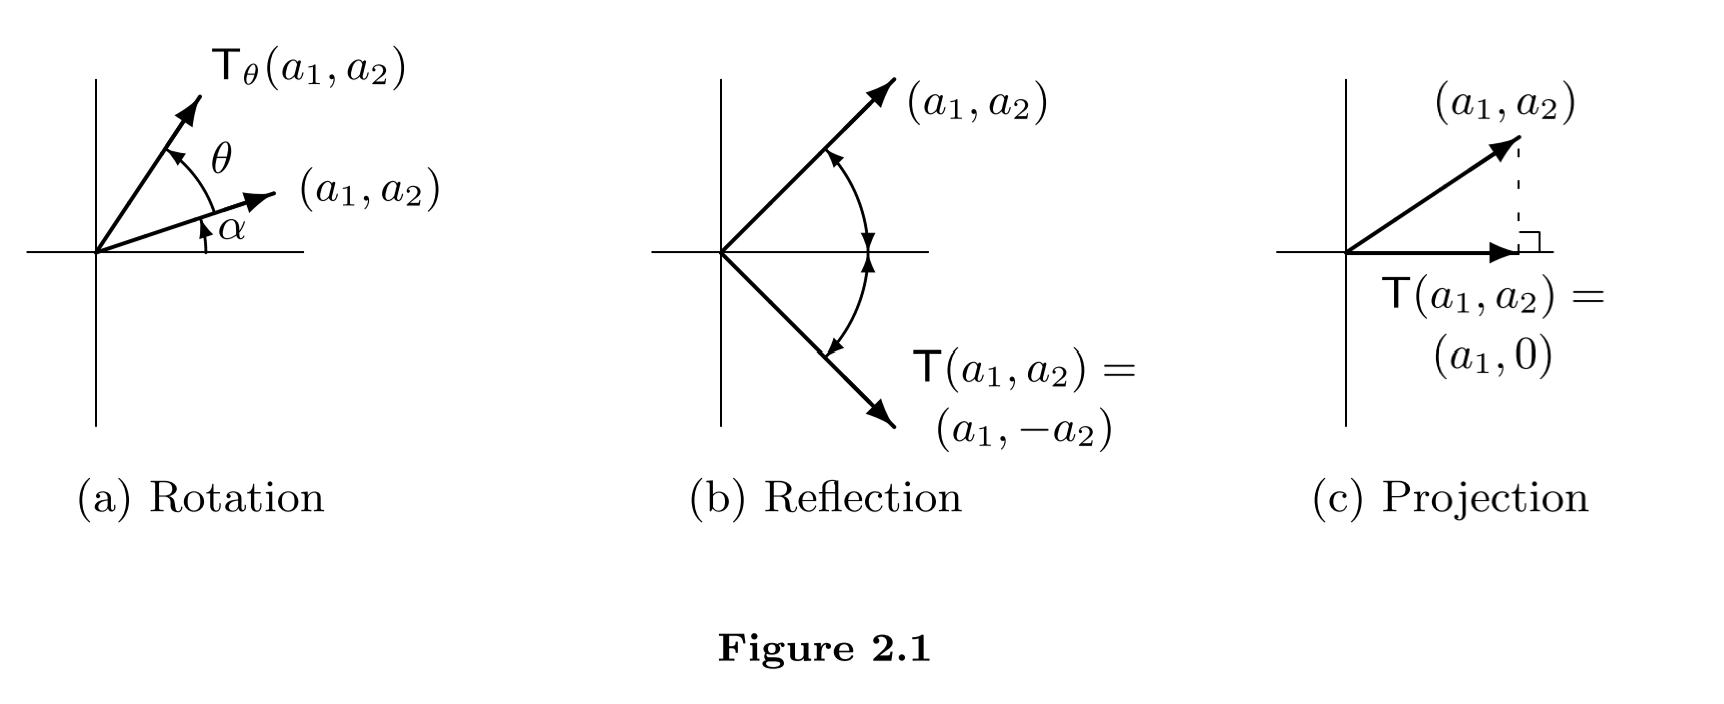
\includegraphics[width=16cm]{images/figure-2-1.png}

\begin{example} \label{example 2.1.2}
For any angle \(\theta\), define \(\T_{\theta} : \SET{R}^2 \to \SET{R}^2\) by the ``rule'':
\(\T_{\theta} (a_1, a_2)\) is the vector obtained by \emph{rotating \((a_1, a_2)\) counterclockwise by \(\theta\)} if \((a_1, a_2) \ne (0, 0)\), and \(\T_{\theta}(0, 0) = (0, 0)\).
Then \(\T_{\theta} : \SET{R}^2 \to \SET{R}^2\) is a \LTRAN{} that is called the \textbf{rotation by \(\theta\)}.

We determine an \emph{explicit formula} for \(\T_{\theta}\).
Fix a nonzero vector \((a_1, a_2) \in \SET{R}^2\).
Let \(\alpha\) be the angle that \((a_1, a_2)\) \emph{makes with the positive \(x\)-axis} (see Figure 2.1(a)),
and let \(r = \sqrt{a_1^2 + a_2^2}\).
Then \(a_1 = r \cos \alpha\) and \(a_2 = r \sin \alpha\).
Also, \(\T_{\theta}(a_1, a_2)\) has length \(r\) and makes an angle \(\alpha + \theta\) with the positive \(x\)-axis.
It follows that
\begin{align*}
    \T_{\theta}(a_1, a_2) & = (r \cos(\alpha + \theta), r \sin(\alpha + \theta)) \\
                         & = (r \cos \alpha \cos \theta - r \sin \alpha \sin \theta,  r \cos \alpha \sin \theta + r \sin \alpha \cos \theta) & \text{by high school algebra} \\
                         & = (a_1 cos \theta - a_2 \sin \theta, a_1 \sin \theta + a_2 \cos \theta). & \text{since \(r \cos \alpha = a_1, r \sin \alpha = a_2\)}
\end{align*}
And by \RMK{2.1.3}, \(\T\) is linear.
\end{example}

\begin{example} \label{example 2.1.3}
Define \(\T : \SET{R}^2 \to \SET{R}^2\) by \(\T(a_1, a_2) = (a_1, -a_2)\).
\(\T\) is called the \textbf{reflection about the \(x\)-axis}.
(See Figure 2.1(b).)
\end{example}

\begin{example} \label{example 2.1.4}
Define \(\T : \SET{R}^2 \to \SET{R}^2\) by \(\T(a_1, a_2) = (a_1, 0)\).
\(\T\) is called the \textbf{projection on the \(x\)-axis} (along \(y\)-axis, see \ADEF{2.2}).
(See Figure 2.1(c).) 
\end{example}

\begin{example} \label{example 2.1.5}
Define \(\T : M_{m \X n}(F) \to M_{n \X m}(F)\) by \(\T(A) = A^\top\), where \(A^\top\) is the transpose of \(A\).
Then \(\T\) is a \LTRAN{} by \EXEC{1.3.3}, since
\begin{align*}
    \T(aA + bB) & = (aA + bB)^\top \\
               & = aA^\top + bB^\top & \text{by \EXEC{1.3.3}} \\
               & = a\T(A) + b\T(B),
\end{align*}
hence \(\T\) is linear by \ATHM{2.1}(b).
\end{example}

\begin{example} \label{example 2.1.6}
Let \(V\) denote the set of all real-valued functions defined on the real line that \emph{have derivatives of every order}.
It is easily shown that \(V\) is a vector space over \(\SET{R}\).
(See \EXEC{1.3.16}.)
Define \(\T : V \to V\) by \(\T(f) = f'\), the derivative of \(f\).
(Note that the input of \(\T\) is itself a function(from \(\SET{R}\) to \(\SET{R}\)); the output of \(\T\) is similar.)
To show that \(\T\) is linear, let \(g, h \in V\) and \(a \in \SET{R}\).
Now
\begin{align*}
    \T(ag + h) & = (ag + h)' \\
              & = ag' + h' & \text{by Calculus} \\
              & = a\T(g) + \T(h).
\end{align*}
So by \ATHM{2.1}(b), \(\T\) is linear.
\end{example}

\begin{example} \label{example 2.1.7}
Let \(V = \mathcal{C}(\SET{R})\), the vector space of all continuous real-valued functions on \(\SET{R}\).
Let \(a, b \in \SET{R}\), \(a < b\).
Define \(\T : V \to \RED{\SET{R}}\) by
\[
    \T(f) = \int_a^b f(t) dt
\]
for all \(f \in V\).
(Note that the input of \(\T\) is a (continuous) function, the output of \(\T\) is the definite integral of that input on the interval \(a, b\).)
Then \(\T\) is a \LTRAN{} because, by Calculus, the definite integral of a linear combination of functions is the same as the linear combination of
the definite integrals of the functions.
\end{example}

\begin{additional definition} \label{adef 2.1}
For vector spaces \(V\) and \(W\) (over common \(F\)), we define the \textbf{identity transformation} \(\ITRANV: V \to \RED{V}\) by \(\ITRANV(x) = x\) for all \(x \in V\) and the \textbf{zero transformation} \(\TZERO: V \to W\) by \(\TZERO(x) = \OW\) for all \(x \in V\).
It is clear that both of these transformations are linear.
We often write \(\mathrm{I}\) instead of \(\ITRANV\).
\end{additional definition}

We now turn our attention \emph{to two very important sets associated with \LTRAN{}s}: the \textbf{range} and \textbf{null space}.
The determination of these sets allows us to examine more closely the \emph{intrinsic} properties of a \LTRAN{}.

\begin{definition} \label{def 2.2}
Let \(V\) and \(W\) be vector spaces, and let \(\T : V \to W\) be linear.
We define the \textbf{null space} (or \textbf{kernel}) \(\NULLT\) of \(\T\) to be the set of all vectors \(x\) in \(V\) such that \(\T(x) = \OW\);
that is, \(\NULLT = \{ x \in V : \T(x) = \OW \}\).

We define the \textbf{range} (or \textbf{image}) \(\RANGET\) of \(\T\) to be the subset of \(W\) consisting of all images (under \(\T\)) of vectors in \(V\);
that is, \(\RANGET = \{ \T(x) : x \in V \}\).
\end{definition}

\begin{example} \label{example 2.1.8}
Let \(V\) and \(W\) be vector spaces, and let \(\ITRANV : V \to V\) and \(\TZERO : V \to W\) be the identity and zero transformations, respectively. Then \(\NULL(\ITRANV) = \{ \OV \}\), \(\RANGE(\ITRANV) = V\), \(\NULL(\TZERO) = V\), and \(\RANGE(\TZERO) = \{ \OW \}\).
\end{example}

\begin{example} \label{example 2.1.9}
Let \(\T : \SET{R}^3 \to \SET{R}^2\) be the \LTRAN{} defined by \(\T(a_1, a_2, a_3) = (a_1 - a_2, 2a_3)\).
It is left as an exercise to verify that
\[
    \NULLT = \{ (a, a, 0) : a \in \SET{R} \} \text{ and } \RANGET = \SET{R}^2.
\].
\end{example}

\begin{remark} \label{remark 2.1.4}
In \EXAMPLE{2.1.8} and \EXAMPLE{2.1.9}, we see that the range and null space of each of the \LTRAN{}s happen to be a \emph{subspace} (of the codomain and domain, respectively).
The next result shows that this is \emph{true in general}.
\end{remark}

\begin{theorem} \label{thm 2.1}
Let \(V\) and \(W\) be vector spaces and \(T : V \to W\) be linear.
Then \(\NULLT\) and \(\RANGET\) are \textbf{subspaces} of \(V\) and \(W\) (over common \(F\)), respectively.
\end{theorem}

\begin{proof}
We prove \(\NULLT\) and \(\RANGET\) are \textbf{subspaces} of \(V\) and \(W\) by showing they satisfy the conditions in \THM{1.3}.

Since by \ATHM{2.1}(a), \(\T(\OV) = \OW\), (by \DEF{2.2}) we have that \(\OV \in \NULLT\).
Let \(x, y \in \NULLT\) and \(c \in F\).
Then
\begin{align*}
    \T(x + y) & = \T(x) + \T(y) & \text{since \(\T\) is linear} \\
              & = \OW + \OW & \text{since \(x, y \in \NULLT\)} \\
              & = \OW,
\end{align*}
so by \DEF{2.2}, \(x + y \in \NULLT\);
and
\begin{align*}
    \T(cx) & = c \T(x) & \text{since \(\T\) is linear} \\
           & = c \OW & \text{since \(x \in \NULLT\)} \\
           & = \OW.
\end{align*}
Hence by \DEF{2.2}, \(cx \in \NULLT\), so that by \THM{1.3} \(\NULLT\) is a subspace of \(V\).

Now for \(\RANGET\), because \(\T(\OV) = \OW\), we have that \(\OV \in \RANGET\).
Now let \(x, y \in \RANGE(T)\) and \(c \in F\).
Then there exist \(u\) and \(w\) in \(V\) such that \(\T(v) = x\) and \(\T(w) = y\).
So \(\T(v + w) = \T(v) + \T(w) = x + y\), and \(\T(cv) = c\T(v) = cx\). Thus \(x + y \in \RANGET\) and \(cx \in \RANGET\), so by \THM{1.3}, \(\RANGET\) is a subspace of \(W\).
\end{proof}

The next theorem provides a method for finding a \emph{spanning set} (\emph{not} necessarily a basis) for the \emph{range} of a \LTRAN{}.
With this accomplished, using the technique of \EXAMPLE{1.6.6} (or \THM{1.9}), it is easy to find a basis, which is a subset of the spanning set, for the \emph{range}.

\begin{theorem} \label{thm 2.2}
Let \(V\) and \(W\) be vector spaces, and let \(\T : V \to W\) be linear.
If \(\beta = \{ v_1, v_2 , ..., v_n \}\) is a \emph{basis} for \(V\), then
\[
    \RANGET = \spann(\T(\beta)) =^{\RED{*}} \spann(\{ \T(v_1), \T(v_2), ..., \T(v_n) \}).
\]
(\RED{*} Note that \(\T(\{ v_1, v_2 , ..., v_n \})\) is just a syntactic sugar for \(\{ \T(v_1), \T(v_2), ..., \T(v_n) \}\).)

Also note that we do \emph{not} say \(\T(\beta)\) is a basis for \(\RANGET\);
we just say it is a generating set for \(\RANGET\).
\end{theorem}

\begin{proof} Clearly (by definition of the ``image'' of an input \(v_i\)) \(\T(v_i) \in \RANGET\) for each \(i\).

So \(\{ \T(v_1), \T(v_2), ..., \T(v_n) \} \subseteq \RANGET\).
Because \(\RANGET\) is a \emph{subspace}, by \THM{1.5}(b), \(\RANGET\) contains \(\spann(\{ \T(v_1 ), \T(v_2), ..., \T(v_n) \}) = \spann(\T(\beta))\).

So we have \(\spann(\T(\beta)) \subseteq \RANGET\).

Now suppose arbitrary \(w \in \RANGET\).
Then \(w = \T(v)\) for some \(v \in V\).
Because \(\beta\) is a basis for \(V\), we have
\[
    v = \sum_{i = 1}^n a_i v_i \text{ for some \(a_1, a_2, ..., a_n \in F\)} \MAROON{(1)}.
\]
Since \(T\) is linear, it follows that
\begin{align*}
    w & = \T(v) \\
      & = \T \bigg(\sum_{i = 1}^n a_i v_i \bigg) & \text{by \MAROON{(1)}} \\
      & = \sum_{i = 1}^n a_i T(v_i), & \text{by \ATHM{2.1}(d)} \\
\end{align*}
which is a linear combination of \(\T(\beta)\), hence \(w \in \spann(\T(\beta))\).
So we have \(\RANGET \subseteq \spann(\T(\beta))\).
Hence \(\RANGET = \spann(\T(\beta))\).
\end{proof}

\begin{remark} \label{remark 2.1.5}
It should be noted that \THM{2.2} is true even if \(\beta\) is infinite, that is, \(\RANGET = \spann(\{ \T(v) : v \in \beta \})\).
(See \EXEC{2.1.34}.)
\end{remark}

\begin{example} \label{example 2.1.10}
Define the linear(need to prove, but trivial) transformation \(T : \mathcal{P}_2(\SET{R}) \to M_{2 \X 2}(\SET{R})\) by
\[
    T(f) = \begin{pmatrix}
        f(1) - f(2) &    0 \\
        0           & f(0)
    \end{pmatrix}.
\]
Since \(\beta = \{1, x, x^2\}\) is a basis for \(\mathcal{P}_2(\SET{R})\), we have
\begin{align*}
    \RANGET & = \spann(\T(\beta)) & \text{by \THM{2.2}} \\
            & = \spann(\{\T(1), \T(x), \T(x^2)\}) & \text{unwrap syntactic sugar} \\
            & = \spann\bigg(\bigg\{
                    \begin{pmatrix}
                        0 & 0 \\
                        0 & 1
                    \end{pmatrix},
                    \begin{pmatrix}
                        -1 & 0 \\
                        0  & 0
                    \end{pmatrix},
                    \begin{pmatrix}
                        -3 & 0 \\
                        0  & 0
                    \end{pmatrix}
                \bigg\}\bigg) \\
            & = \spann\bigg(\bigg\{
                    \begin{pmatrix}
                        0 & 0 \\
                        0 & 1
                    \end{pmatrix},
                    \begin{pmatrix}
                        -1 & 0 \\
                        0  & 0
                    \end{pmatrix}
                \bigg\}\bigg) & \text{by extract subset as basis}
\end{align*}
Thus we have found a basis for \(\RANGET\), and so \(\dim(\RANGET) = 2\).

Now suppose that we want to find a basis for \(\NULLT\).
Note that \(f \in \NULLT\) if and only if \(T(f) = O_{2 \X 2}\), the \(2 \X 2\) zero matrix.
That is, \(f \in \NULLT\) if and only if
\[
    \begin{pmatrix}
        f(1) - f(2) & 0 \\
        0 & f(0)
    \end{pmatrix}
    = \begin{pmatrix}
        0 & 0 \\
        0 & 0
    \end{pmatrix}.
\]
Now express \(f(x) = a + bx + cx^2\) for any \(a, b, c \in \SET{R}\).
If \(f(1) - f(2) = 0\) and \(f(0) = 0\), then we have \(0 = f(1) - f(2) = (a + b + c) - (a + 2b + 4c) = -b - 3c\), or \(b = -3c\);
and \(0 = f(0) = a + 0 + 0 = a\).
So \(f\) must have the form that \(f(x) = 0 + (-3c) x + c x^2 = c(-3x + x^2)\).
Hence \(\NULLT = \{ c(-3x + x^2) : c \in \SET{R} \}\), and trivially the basis is \(\{ -3x + x^2 \}\), hence \(\NULLT\) has dimension \(1\).
\end{example}

\begin{remark} \label{remark 2.1.6}
Note that in \EXAMPLE{2.1.10},
\[
    \dim(\NULLT) + \dim(\RANGET) = 1 + 2 = 3 = \dim(\mathcal{P}_2(\SET{R})).
\]
In \THM{2.3}, we see that a similar result is \emph{true in general}.
\end{remark}

As in \CH{1}, we ``measure the size'' of a subspace by its dimension.
The null space and range are so important that we \emph{attach special names} to their respective dimensions.

\begin{definition} \label{def 2.3}
Let \(V\) and \(W\) be vector spaces, and let \(\T : V \to W\) be linear.
If \(\NULLT\) and \(\RANGET\) are finite-dimensional, then we define the \textbf{nullity} of \(\T\), denoted \(\nullityT\), and the \textbf{rank} of \(\T\), denoted \(\rankT\),
to be the dimensions of \(\NULLT\) -- or \(\dim(\NULLT)\) -- and \(\RANGET\) -- or \(\dim(\RANGET)\) -- respectively.
\end{definition}

\begin{remark} \label{remark 2.1.7}
Reflecting on the action of a \LTRAN{}, we see intuitively that \textbf{the larger the nullity, the smaller the rank}.
In other words, the more vectors that are carried into \(\OW\), the smaller the range.
The same heuristic reasoning tells us that \textbf{the larger the rank, the smaller the nullity}.
This balance between rank and nullity is made precise in the next theorem, appropriately called \textbf{the dimension theorem}.
\end{remark}

\begin{theorem} [Dimension Theorem] \label{thm 2.3}
Let \(V\) and \(W\) be vector spaces, and let \(\T : V \to W\) be linear.
If \(V\) is \emph{finite}-dimensional, then
\[
    \nullityT + \rankT = \dim(V).
\]
\end{theorem}

\begin{proof}
Suppose that \(\dim(V) = n, \nullityT = k\), and \(\{ v_1, v_2, ..., v_k \}\) is a basis for \(\NULLT\).
By \CORO{1.11.1}, (since \(\NULLT\) is a subspace of \(V\),) we may extend \(\{ v_1, v_2, ..., v_k \}\) to a basis \(\beta = \{ v_1, v_2, ..., v_k, v_{k +1}, ..., v_n \}\) for \(V\).
We claim that
\[
    S = \{ \T(v_{k + l}), \T((v_{k + 2}), ..., \T(v_n) \}
\]
is a basis for \(\RANGET\).

But first, we need to show that \(\T(v_{k + 1}), ..., \T(v_n)\) are all \textbf{distinct}. (s.t. \(S\) has \(n - k\) elements.)

For the sake of contradiction, suppose not.
Then there exists \(i \ne j\), \(k + 1 \le i \le n, k + 1 \le j \le n\), s.t. \(\T(v_i) = \T(v_j)\).
And
\begin{align*}
             & \T(v_i) = \T(v_j) \\
    \implies & \T(v_i) - \T(v_j) = \OW \\
    \implies & \T(v_i - v_j) = \OW & \text{by \ATHM{2.1}(c)} \\
    \implies & v_i - v_j \in \NULLT & \text{by \DEF{2.2}} \\
    \implies & v_i - v_j \in \spann(\{ v_1, ..., v_k \}) \\
    \implies & \{ v_1, ..., v_k, v_i - v_j \} \text{ is \LDP{} } & \text{by \THM{1.7}}
\end{align*}
So we have a \emph{nontrivial} combination \(\OV = a_1 v_1 + ... + a_k v_k + a (v_i - v_j)\).
Note that \(a\) cannot be zero, otherwise one of \(a_1, ..., a_k\) must be nonzero and we have nontrivial representation using \(v_1, ..., v_k\), which contradicts that \(v_1, ..., v_k\) is \LID{}.
But then \(\OV = a_1 v_1 + ... + a_k v_k + a (v_i - v_j) = a_1 v_1 + ... + a_k v_k + a v_i - a v_j\), and that still implies \(\{ a_1, a_2, ..., a_k, a_i, a_j \}\) are \LDP{}, which is a contradiction since it is a subset of a basis (hence \LID{}) of \(V\).
So \(\T(v_{k + 1}), \T(v_{k + 2}), ..., \T(v_n)\) must be all distinct, so \(S\) really has \(n - k\) elements.

Go back to the consideration of \(S\).
First we prove that \(S\) generates \(\RANGET\).
Using \THM{2.2} (and \(\beta\) is a basis for \(V\)) and \RED{the fact that} \(\T(v_i) = \OW\) for \(1 \le i \le k\), we have
\begin{align*}
    \RANGET & = \spann(\{ \T(v_1), \T(v_2), ..., \T(v_{k}), \T(v_{k + 1}, ..., T(v_n) \}) & \text{by \THM{2.2}} \\
            & = \spann(\{ \OW, \OW, ..., \OW, \T(v_{k + 1}), ..., \T(v_{n}) \}) & \text{using the fact} \\
            & = \spann(\{ \OW, \T(v_{k + 1}), ..., \T(v_{n}) \}) & \text{equal by set theory} \\
            & = \spann(\{ \T(v_{k + 1}), ..., \T(v_{n}) \}) & \text{of course, by \CH{1}} \\
            & = \spann(S).
\end{align*}

Now we prove that \(S\) is \LID{}.
So suppose that
\[
    \sum_{i = k + 1}^n b_i T(v_i) = \OW \text{ for some scalars \(b_{k + 1}, ..., b_n \in F\)}. \MAROON{(1)}
\]
Using the fact that \(T\) is linear, by \ATHM{2.1}(d), we have
\[
    T\bigg( \sum_{i = k + 1}^n b_i v_i \bigg) = \OW.
\]
So by \DEF{2.2},
\[
    \sum_{i = k + 1}^n b_i v_i \in \NULLT.
\]
Hence \(LHS\) can be represented as a linear combination of the basis of \(\NULLT\), that is,
\[
    \sum_{i = k + 1}^n b_i v_i = \sum_{i = 1}^k c_i v_i,
\]
hence
\[
    \sum_{i = 1}^k (-c_i) v_i + \sum_{i = k + 1}^n b_i v_i = \OV.
\]
But \(\beta = \{ v_1, ..., v_k, v_{k + 1}, ..., v_n \}\) is known to be the basis of \(V\) (hence is \LID{}), so we have \(c_i\) for \(i = 1, ..., k\) and \(b_i\) for \(i = k + 1, ..., n\) are all equal to zero.
And in particular, \(b_{k + 1} = ... = b_n = 0\).
So by \MAROON{(1)}, \(S\) is \LID{}.

Hence we know \(S\) generates \(\RANGET\) and is \LID{}, so \(S\) is a basis for \(\RANGET\).
Therefore \(\rankT = \#S = n - k\), there for \(\nullityT + \rankT = k + (n - k) = n = \dim(V)\).
\end{proof}

\begin{note}
If we apply the dimension theorem to the \LTRAN{} \(\T\) in \EXAMPLE{2.1.9}, we have that \(\nullityT + 2 = 3\), so \(\nullityT = 1\).
\end{note}

\begin{remark} \label{remark 2.1.8}
The reader should review the concepts of \emph{``one-to-one'' and ``onto''}.
Interestingly, for a \LTRAN{}, both of these concepts are \emph{intimately connected} to the rank and nullity of the transformation.
This is demonstrated in the next two theorems.
\end{remark}

\begin{theorem} \label{thm 2.4}
Let \(V\) and \(W\) be vector spaces, and let \(\T : V \to W\) be linear.
Then \(\T\) is one-to-one \emph{if and only if} \(\NULLT = \{ \OV \}\).
\end{theorem}

\begin{proof} \ 

\(\Longrightarrow\): Suppose \(\T\) is one-to-one, we have to show \(\NULLT = \{ \OV \}\).
So let \(x \in \NULLT\), we have to show \(x = \OV\).
By \DEF{2.2}, we have \(\T(x) = \OW\).
But by \ATHM{2.1}(a), \(\T(\OV) = \OW\).
So we have \(\T(x) = \T(\OV)\).
By definition of one-to-one, that implies \(x = \OV\).

\(\Longleftarrow\):
Suppose \(\NULLT = \{ \OV \}\), we have to show \(\T\) is one-to-one.
So suppose arbitrary \(x_1, x_2\) s.t. \(\T(x_1) = \T(x_2)\), we have to show \(x_1 = x_2\).
Then we have
\begin{align*}
             & \T(x_1) = \T(x_2) \\
    \implies & \T(x_1) - \T(x_2) = \OW \\
    \implies & \T(x_1 - x_2) = \OW & \text{by \ATHM{2.1}(c)} \\
    \implies & x_1 - x_2 \in \NULLT & \text{by \DEF{2.2}} \\
    \implies & x_1 - x_2 = \OV & \text{since \(\NULLT = \{ \OV \}\)} \\
    \implies & x_1 = x_2.
\end{align*}
So by definition, \(\T\) is one-to-one.
\end{proof}

\begin{remark} \label{remark 2.1.9}
\THM{2.4} is true even if \(V\) is \emph{infinite}-dimensional.
\end{remark}

\begin{note}
Observe that \THM{2.4} allows us to conclude that the transformation defined in \EXAMPLE{2.1.9} is not one-to-one since \(\NULLT \ne \{ \OV \}\).
\end{note}

Surprisingly, the conditions of one-to-one and onto are \textbf{equivalent} in an important special case; that is, when the domain and codomain of the \LTRAN{} have the same \emph{finite} dimensions.

\begin{theorem} \label{thm 2.5}
Let \(V\) and \(W\) be \emph{finite}-dimensional vector spaces \textbf{of equal dimension}, and let \(\T : V \to W\) be linear.
Then the following are equivalent.
\begin{enumerate}
\item \(\T\) is one-to-one.
\item \(T\) is onto.
\item \(\rankT = \dim(V)\).
\end{enumerate}
\end{theorem}

\begin{proof}
From the dimension theorem \THM{2.3}, we have
\[
    \nullityT + \rankT = \dim(V). \MAROON{(1)}
\]
And we have
\begin{align*}
         & \BLUE{\T \text{ is one-to-one }} \\
    \iff & \NULLT = \{ \OV \} & \text{by \THM{2.4}} \\
    \iff & \nullityT = 0 & \text{by \DEF{2.3}} \\
    \iff & \BLUE{\rankT = \dim(V)} & \text{by \MAROON{(1)}} \\
    \iff & \rankT = \dim(W) & \text{since \(V\) and \(W\) have same finite-dimension} \\
    \iff & \dim(\RANGET) = \dim(W) & \text{by \DEF{2.3}} \\
    \iff & \RED{*} \BLUE{\T \text{ is onto.}}
\end{align*}
So we have shown (a), (b), and (c) are equivalent.

\RED{*}: For the last step, since by \THM{2.1}, \(\RANGET\) is a subspace of \(W\), and has the same dimension with \(W\), by \THM{1.11}, \(\RANGET = W\), which implies \(\T\) is onto.
\end{proof}

\begin{remark} \label{remark 2.1.10}
We note that if \(V\) is \emph{not} finite-dimensional and \(\T : V \to V\) is linear, then \textbf{it does not follow that} one-to-one and onto are equivalent.
(See \EXEC{2.1.15}, \EXEC{2.1.16}, and \EXEC{2.1.21}.)

Note that the \textbf{linearity} of \(\T\) in \THM{2.4} and \THM{2.5} is essential, for it is easy to construct examples of functions from \(\SET{R}\) into \(\SET{R}\) that are not one-to-one, but
are onto, and vice versa.
\end{remark}

\begin{example} \label{example 2.1.11}
Let \(\T : \mathcal{P}_2(\SET{R}) \to \mathcal{P}_3(\SET{R})\) be the \LTRAN{} defined by
\[
    \T(f(x)) = 2f'(x) + \int_0^x 3f(t) dt.
\]
(Note that integration will make the degree increase by \(1\), so the codomain has one more dimension than domain.)

Now
\begin{align*}
    \RANGET & = \spann(\{ \T(1), \T(x), \T(x^2) \}) & \text{by \THM{2.2}} \\
            & = \spann(\{ 3x, 2 + \frac{3}{2} x^2, 4x + x^3 \}).
\end{align*}
Since \(\{ 3x, 2 + \frac{3}{2} x^2, 4x + x^3 \}\) is \LID{}, \(\rankT = 3\).
Since the dimension of the codomain \(\dim(\mathcal{P}_3(\SET{R})) = 4\), \(\T\) is not onto.
From the dimension theorem, \(3 = \dim(\mathcal{P}_2(\SET{R})) = \nullityT + \rankT = \nullityT + 3\).
So \(\nullityT = 0\), and therefore, \(\NULLT = \{ \OV \}\).
We conclude from \THM{2.4} that \(\T\) is one-to-one.
\end{example}

\begin{example} \label{example 2.1.12}
Let \(\T : F^{\RED{2}} \to F^{\RED{2}}\) be the \LTRAN{} defined by
\[
    \T(a_1, a_2) = (a_1 + a_2, a_1).
\]
It is easy to see that \(\NULLT = \{ \OV \}\);
so by \THM{2.4} \(\T\) is one-to-one.
Hence \THM{2.5} tells us that (since domain and codomain of \(\T\) have same finite dimension,) \(\T\) must be onto.
\end{example}

\begin{note}
In \EXEC{2.1.14}, it is stated that if \(\T\) is linear and one-to-one, then a subset \(S\) (of domain of \(\T\)) is \LID{} if and only if \(\T(S)\) (, a subset of codomain of \(\T\),) is \LID{}.
The next example illustrates the use of this result.
\end{note}

\begin{example} \label{example 2.1.13}
Let \(\T : \mathcal{P}_2(\SET{R}) \to \SET{R}^3\) be the \LTRAN{} defined by
\[
    \T(a_0 + a_1 x + a_2 x^2) = (a_0, a_1, a_2).
\]
Clearly \(\T\) is linear and one-to-one(and onto).
Let \(S = \{ 2 - x + 3x^2, x + x^2, 1 - 2x^2 \}\).
Then \(S\) is \LID{} in \(\mathcal{P}_2(\SET{R})\) because (by \EXEC{2.1.14} and)
\[
    \T(S) = \{ (2, -1, 3), (0, 1, 1), (1, 0, -2) \}
\]
is \LID{} in \(\SET{R}^3\).
\end{example}

\begin{remark} \label{remark 2.1.11}
In \EXAMPLE{2.1.13}, we \emph{transferred a property} from the vector space of polynomials (with dimension \(3\)) to a property in the vector space of \(3\)-tuples (also with dimension \(3\)).
This technique is exploited more fully later.
(See \SEC{2.4}).
\end{remark}

\begin{note}
\EXEC{2.1.14} 的用意是,你想看一坨向量是否線性獨立,但(可能)很難算,於是你把它們用一個符合一對一的線性函數\ \(\T\) 變換成另一個空間的一坨向量,並且在該空間計算向量是否線性獨立(可能)比較好算;算完後再根據\ \EXEC{2.1.14} 就可知道原本那陀向量是否線性獨立了。
\end{note}

One of the most important properties of a \LTRAN{} is that \textbf{it is completely determined by its action on a basis}.
This result, which follows from the next theorem and corollary, is used frequently throughout the book.

\begin{theorem} \label{thm 2.6}
Let \(V\) and \(W\) be vector spaces over \(F\), and suppose that \(\{ v_1, v_2, ..., v_n \}\) is a basis for \(V\).
Then given any \(n\) vectors \(w_1, w_2, ..., w_n \in W\), there \textbf{exists exactly one} \LTRAN{} \(\T : V \to W\) such that \(\T(v_i) = w_i\) for \(i= 1, 2, ..., n\).
\end{theorem}

\begin{remark} \label{remark 2.1.12}
The purpose of \THM{2.6} is that, if \(V\) and \(W\) are finite vector spaces, and given any \emph{basis} \(\{ v_1, v_2, ..., v_n \}\) for \(V\), and the ``wanted'' corresponding output \(\{ w_1, w_2, ..., w_n \}\) in \(W\), we \emph{can always find} a \LTRAN{} from \(V\) to \(W\) that satisfies the requirement.
Furthermore, the found \LTRAN{} \emph{is unique}.

Hence we can just use a ``mapping'' \(v_1 \to w_1, v_1 \to w_2, ..., v_n \to w_n\) to \emph{identify} the one and only one \LTRAN{}, so this identification is \emph{well-defined}.
And in later sections, we will learn that the ``mapping'' can be represented using \textbf{matrix}!
And that ultimately implies that every \LTRAN{} corresponds to a unique matrix.
\end{remark}

\begin{proof}
Let \(\{ v_1, v_2, ..., v_n \}\) be a basis for \(V\), and let \(w_1, w_2, ..., w_n\) be vectors in \(W\).

We first prove the existence of \(\T\) such that \(\T\) is linear and \(\T(v_i) = w_i\) for \(i = 1, 2, ..., n\).

So suppose arbitrary \(x \in V\).
Then (since \(\{ v_1, ..., v_n \}\) is a basis for \(V\),)
\[
    x = \sum_{i = 1}^n a_i v_i,
\]
where \(a_1, ..., a_n\) are \textbf{unique} scalars.
Now we prove by construction by defining \(\T\), using this scalars \emph{that depend on \(x\)}:
\[
    \T : V \to W \text{ by } \T(x) = \T\bigg(\sum_{i = 1}^n a_i v_i\bigg) = \sum_{i = 1}^n a_i w_i. \MAROON{(1)}
\]
Then of course \(\T\) is really a \emph{well-defined} function, since
\BLUE{(1)} it's output is a linear combination of \(W\)'s vectors, which must be in \(W\);
\BLUE{(2)} And since for any \(x\) in \(V\), the corresponding scalars \(a_1, ..., a_n\) are \emph{unique}, hence the output of \(\T\) is also unique.
Also note that \MAROON{(1)} is \textbf{not} actually a ``formula'' with ``constant scalars'' \(a_1, ..., a_n\), since \(a_1, ..., a_n\) are determined by (or dependent on) the given \(x\), so they are ``dynamic''.

Then we have to show (a) \(\T\) is linear; (b) \(\T(v_i) = w_i\) for all \(i = 1, ..., n\):
\begin{enumerate}
\item
We will use \ATHM{2.1}(b) to show \(\T\) is linear.
So suppose \(u, v \in V\), and \(d \in F\).
Then (similarly as \(x \in V\),) we may write
\[
    u = \sum_{i = 1}^n b_i v_i \text{ and } v = \sum_{i = 1}^n c_i v_i \MAROON{(2)}
\]
for some (unique) scalars \(b_1, b_2, ..., b_n\) and \(c_1, c_2, ..., c_n\).
Thus
\begin{align*}
    d u + v & = d \sum_{i = 1}^n b_i v_i + \sum_{i = 1}^n c_i v_i \\
            & = \sum_{i = 1}^n (db_i + c_i) v_i \MAROON{(3)} & \text{by rules of finite summation}
\end{align*}
So
\begin{align*}
    \T(du + v) & = \T\bigg( \sum_{i = 1}^n (db_i + c_i) v_i \bigg) & \text{by \MAROON{(3)}} \\
               & = \sum_{i = 1}^n (db_i + c_i) w_i \\
               & \text{\ \ \ \ \ \ (by \MAROON{(1)}; note that now the corresponding} \\
               & \text{\ \ \ \ \ \ \ \ scalars \(a_1, ..., a_n\) in \MAROON{(1)}} \\
               & \text{\ \ \ \ \ \ \ \ are \(d b_1 + c_1, ..., d b_n + c_n\))} \\
               & = d \sum_{i = 1}^n b_i w_i + \sum_{i = 1}^n c_i w_i & \text{by rules of finite summation} \\
               & = d \T\bigg( \sum_{i = 1}^n b_i v_i \bigg) + \T\bigg( \sum_{i = 1}^n c_i v_i \bigg) & \text{again by \MAROON{(1)}} \\
               & = d \T(u) + \T(v), & \text{by \MAROON{(2)}}
\end{align*}
hence \(\T\) is linear.

\item
For \(v_i\) where \(i = 1, ..., n\):
\begin{align*}
    \T(v_i) & = \T(0 v_1 + ... + 1 v_i + ... + 0 v_n) & \text{in particular} \\
            & = 0 w_1 + ... + 1 w_i + ... + 0 w_n & \text{by \MAROON{(1)}, and expand summation} \\
            & = w_i.
\end{align*}
\end{enumerate}
Hence \(\T\) satisfies the two requirements, so the existent part is proved.

Now we have to show \(\T\) is unique.
So suppose \(\U\) is also linear s.t. \(\U(v_i) = w_i\) for \(i = 1, ..., n\).
We have to show \(\U = \T\);
that is, (by definition of function equality,) we have to show \(\forall x \in V, \U(x) = \T(x)\).

But for each \(x \in V\), where again we represent \(x = \sum_{i = 1}^n a_i v_i\) for unique scalars \(a_1, ..., a_n\) \MAROON{(4)},
\begin{align*}
    \U(x) & = \U\bigg(\sum_{i = 1}^n a_i v_i\bigg) & \text{by \MAROON{(4)}}\\
           & = \sum_{i = 1}^n a_i \U(v_i) & \text{since \(\U\) is linear} \\
           & = \sum_{i = 1}^n a_i w_i & \text{since also \(\U(v_i) = w_i\)} \\
           & = \T\bigg(\sum_{i = 1}^n a_i v_i\bigg) & \text{by \MAROON{(1)}} \\
           & = \T(x). & \text{by \MAROON{(4)}}
\end{align*}
So \(\U = \T\), as desired.
\end{proof}

\begin{note}
There is \href{https://www.youtube.com/watch?v=gAlUekIYKLA&ab_channel=DrPeyam}{another proof} for \THM{2.6}.
\end{note}

\begin{corollary} \label{corollary 2.6.1}
\sloppy Let \(V\) and \(W\) be vector spaces, and suppose that \(V\) has a finite basis \(\{ v_1, v_2, ..., v_n \}\).
If \(\U, \T : V \to W\) are linear and \(\U(v_i) = \T(v_i)\) for \(i = 1, 2, ..., n\), then \(\U = \T\).
\end{corollary}

\begin{proof}
Well, since by \THM{2.6} \emph{the} \LTRAN{} that satisfies the mapping \(v_i \to w_i\) for \(i = 1, 2, ... n\) is unique,
and both \(\U, \T\) are linear and satisfy the mapping, hence they are equal to that unique \LTRAN{} hence are equal to each other.
\end{proof}

\begin{example} \label{example 2.1.14}
Let \(\T : \SET{R}^2 \to \SET{R}^2\) be the \LTRAN{} defined by
\[
    \T(a_1, a_2) = (2 a_2 - a_1, 3 a_1),
\]
Then \(\T(1, 2) = (3, 3)\) and \(\T(1, 1) = (1, 3)\), where \(\{ (1, 2), (1, 1) \}\) is a basis for \(\SET{R}^2\).
Now suppose that \(\U : \SET{R}^2 \to \SET{R}^2\) is linear.
If we know that \(\U(1, 2) = (3, 3)\) and \(\U(1, 1) = (1, 3)\), then by \CORO{2.6.1}, \(\U = \T\).
\end{example}

\exercisesection

\begin{exercise} \label{exercise 2.1.1}
Label the following statements as true or false.
In each part, \(V\) and \(W\) are \textbf{finite}-dimensional vector spaces (over common \(F\)), and \(\T\) is a function from \(V\) to \(W\).
\begin{enumerate}
\item If \(\T\) is linear, then \(\T\) preserves sums and scalar products.
\item If \(\T(x + y) = \T(x) + \T(y)\). then \(\T\) is linear.
\item \(\T\) is one-to-one if and only if the only vector \(x\) such that \(\T(x) = \OW\) is \(x = \OV\).
\item If \(\T\) is linear, then \(\T(\OV) = \OW\).
\item If \(\T\) is linear, then \(\nullityT + \rankT = \dim(W)\).
\item If \(\T\) is linear, then \(\T\) carries \LID{} subsets of \(V\) onto \LID{} subsets of \(W\).
\item If \(\T, \U : V \to W\) are both linear and agree on a basis for \(V\), then \(\T = \U\).
\item Given \(x_1, x_2 \in V\) and \(y_1, y_2 \in W\), there exists a \LTRAN{} \(\T : V \to W\) such that \(\T(x_1) = y_1\) and \(\T(x_2) = y_2\).
\end{enumerate}
\end{exercise}

\begin{proof} \ 
\begin{enumerate}
\item I really don't know what does the problem want to say, but others say it's true.
\item No, \(\T\) must also need to satisfy \DEF{2.1}(b).
\item False, that is true (by \THM{2.4}) only when we know \(\T\) is linear.
\item True by \ATHM{2.1}(a).
\item False, by \THM{2.3}, \(\nullityT + \rankT = \dim(V)\).
\item False, zero transformation, which is linear, carries all vectors into \(\OW\), which is itself \LDP{}.
    But this is true if \(\T\) is also one-to-one, see \EXEC{2.1.14}.
\item True by \THM{2.6}(or \CORO{2.6.1}).
\item False.
    We can easily find a counterexample when \(x_1, x_2\) are \LDP{}: Let \(V = W = \SET{R}^2\) and \(x_1 = (1, 0), x_2 = (2, 0), y_1 = (1, 0), y_2 = (0, 1)\).
    Then suppose arbitrary \(\T : V \to W\) s.t. \(\T\) is linear, and suppose \(\T(1, 0) = (1, 0)\), that is, \(\T(x_1) = y_1\).
    Then
    \begin{align*}
        \T(x_2) & = \T(2, 0) \\
                & = \T(2(1, 0)) \\
                & = 2\T(1, 0) & \text{since \(\T\) is linear} \\
                & = 2(1, 0) & \text{by supposition} \\
                & = (2, 0) \ne (0, 1) = y_2,    
    \end{align*}
    so any linear \(\T\) can never satisfy the requirement.
\end{enumerate}
\end{proof}

\begin{note}
Exercises 2 - 5 are calculation problems, it's good practice, but it's painful using \LaTeX, skip.
\end{note}

\setcounter{exercise}{5}

\begin{exercise} \label{exercise 2.1.6}
\(\T : M_{n \X n}(F) \to F\) defined by
\[
    \T(A) = \TRACE(A) = \sum_{i = 1}^n A_{ii}.
\]
\end{exercise}

\begin{proof}
\(\NULLT\) is the set of all \(n \X n\) matrices with trace equal to \(0\).
By \ATHM{1.19}(a), \(\nullityT = n^2 - 1\).
And it's trivial that \(\rankT = 1\).
So \(\dim(M_{n \X n}(F)) = n^2 = (n^2 - 1) + 1 = \nullityT + \rankT\), as desired.
And since \(\NULLT \ne \{ \OV \}\), by \THM{2.4}, \(\T\) is not one-to-one.
And since \(\rankT = \dim(W)\), which implies \(\RANGET = W\), \(\T\) is onto.
\end{proof}

\begin{exercise} \label{exercise 2.1.7}
Prove properties 1, 2, 3, and 4 on page 65.
\end{exercise}

\begin{proof}
See \ATHM{2.1}.
\end{proof}

\begin{exercise} \label{exercise 2.1.8}
Prove rotation, reflection, and projection on \EXAMPLE{2.1.2}, \EXAMPLE{2.1.3} are linear.
\end{exercise}

\begin{proof} \ 

\begin{enumerate}
\item
By \EXAMPLE{2.1.2}, given any \(\theta\), we have rotation formula
\[
    \T_{\theta}(a_1, a_2) = (a_1 \cos \theta - a_2 \sin \theta, a_1 \sin \theta + a_2 \cos \theta).
\]
And
\begin{align*}
    & \ \T_{\theta}(c(a_1, a_2) + (b_1, b_2)) \\
    & = \T_{\theta}(ca_1 + b_1, ca_2 + b_2) \\
    & \text{\ \ \ \ \ \ (combining coordinates)} \\
    & = \big( (ca_1 + b_1) \cos \theta - (ca_2 + b_2) \sin \theta, (ca_1 + b_1) \sin \theta + (ca_2 + b_2) \cos \theta \big) \\
    & \text{\ \ \ \ \ \ (by def of \(\T_{\theta}\))} \\
    & = c(a_1 \cos \theta - a_2 \sin \theta, a_1 \sin \theta + a_2 \cos \theta) + (b_1 \cos \theta - b_2 \sin \theta, b_1 \sin \theta + b_2 \cos \theta) \\
    & \text{\ \ \ \ \ \ (splitting coordinates)} \\
    & = c\T(a_1, a_2) + \T(b_1, b_2) \\
    & \text{\ \ \ \ \ \ (by def of \(\T_{\theta}\))}
\end{align*}
So by \ATHM{2.1}(b), \(\T\) is linear.


\item
By \EXAMPLE{2.1.3}, the reflection (about \(x\)-axis) is
\[
    \T(a_1, a_2) = (a_1, -a_2).
\]
Then
\begin{align*}
    & \ \T(c(a_1, a_2) + (b_1, b_2)) \\
    & = \T(ca_1 + b_1, ca_2 + b_2) \\
    & = (ca_1 + b_1, -(ca_2 + b_2)) & \text{by def of \(\T\)} \\
    & = c(a_1, -a_2) + (b_1, -b_2) & \text{splitting coordinates} \\
    & = c\T(a_1, a_2) + \T(b_1, b_2), & \text{by def of \(T\)}
\end{align*}
So by \ATHM{2.1}(b), \(\T\) is linear.

\item
By \EXAMPLE{2.1.4}, the projection (on \(x\)-axis) is
\[
    \T(a_1, a_2) = (a_1, 0).
\]
Then
\begin{align*}
    & \ \T(c(a_1, a_2) + (b_1, b_2)) \\
    & = \T(ca_1 + b_1, ca_2 + b_2) \\
    & = (ca_1 + b_1, 0) & \text{by def of \(\T\)} \\
    & = c(a_1, 0) + (b_1, 0) & \text{splitting coordinates} \\
    & = c\T(a_1, a_2) + \T(b_1, b_2), & \text{by def of \(T\)}
\end{align*}
So by \ATHM{2.1}(b), \(\T\) is linear.
\end{enumerate}
\end{proof}

\begin{exercise} \label{exercise 2.1.9}
In this exercise, \(\T : \SET{R}^2 \to \SET{R}^2\) is a \emph{function}.
For each of the following parts, state why \(\T\) is \emph{not} linear.
\begin{enumerate}
\item \(\T(a_1 , a_2) = (1, a_2)\)
\item \(\T(a_1, a_2) = (a_1, a_1^2)\)
\item \(\T(a_1, a_2) = (\sin a_1, 0)\)
\item \(\T(a_1, a_2) = (\abs{a_1}, a_2)\)
\item \(T(a_1, a_2) = (a_1 + 1, a_2)\)
\end{enumerate}
\end{exercise}

\begin{proof}
By \RMK{2.1.3}, it is immediately seen that all of them are \emph{not} linear.
The particular reasons are:
\begin{enumerate}
\item \(T(0, 0) = (1, 0) \ne \OW\), violating \ATHM{2.1}(a) hence is not linear.
\item \(\T((1, 0) + (1, 0)) = \T(2, 0) = (2, 4)\), but \(\T(1, 0) + \T(1, 0) = (1, 1) + (1, 1) = (2, 2) \ne (2, 4)\), violating \DEF{2.1}(a).
\item \(\T((x, 0) + (y, 0)) = \T(x + y, 0) = (\sin (x + y), 0) = (\sin x \cos y + \cos x \sin y, 0)\) \MAROON{(1)},
    but \(\T(x, 0) + \T(y, 0) = (\sin x, 0) + (\sin y, 0) = (\sin x + \sin y, 0)\),
    which is not necessarily equal to \MAROON{(1)}, so \DEF{2.1}(a) is violated.
\item \(\T(-1(-5, 0)) = \T(5, 0) = (5, 0)\) but \(-1\T(-5, 0) = -1(5, 0) = (-5, 0)\), so \DEF{2.1}(b) is violated.
\item \(\T(0, 0) = (1, 0) \ne \OW\), violating \ATHM{2.1}(a), hence is not linear.
\end{enumerate}
\end{proof}

\begin{exercise} \label{exercise 2.1.10}
Suppose that \(\T : \SET{R}^2 \to \SET{R}^2\) is \emph{linear}, \(\T(1, 0) = (1, 4)\), and \(\T(1, 1) = (2, 5)\).
What is \(\T(2, 3)\)?
Is \(\T\) one-to-one?
\end{exercise}

\begin{proof}
Since \(\{ (1, 0), (1, 1) \}\) is (trivially) a basis for \(\SET{R}^2\), by \THM{2.6} the \(\T\) is \emph{already uniquely determined}.
And
\begin{align*}
    \T(2, 3) & = \T(-1(1, 0) + 3(1, 1)) & \text{of course} \\
             & = -1\T(1, 0) + 3\T(1, 1) & \text{since \(\T\) is linear} \\
             & = -1(1, 4) + 3(2, 5) \\
             & = (5, 11).
\end{align*}
Now by \THM{2.2}, \(\RANGET = \spann(\{ \T(1, 0), \T(1, 1) \}) = \spann(\{ (1, 4), (2, 5) \}\).
Since \(\{ (1, 4), (2, 5) \}\) is \LID{}, it is a basis for \(\RANGET\), hence \(\rankT = 2\).
By \THM{2.3}, \(\nullityT = \dim(V) - \rankT = 2 - 2 = 0\), so \(\NULLT = \{ \OV \}\);
by \THM{2.4}, \(\T\) is one-to-one.
(Also since domain and codomain of \(\T\) have same finite dimension, by \THM{2.5} \(\T\) is also onto.)
\end{proof}

\begin{exercise} \label{exercise 2.1.11}
Prove that there exists a \LTRAN{} \(\T : \SET{R}^2 \to \SET{R}^3\) such that \(\T(1, 1) = (1, 0, 2)\) and \(\T(2, 3) = (1, -1, 4)\).
What is \(\T(8, 11)\)?
\end{exercise}

\begin{proof}
Similar to previous exercise, \(\{ (1, 1), (2, 3) \}\) is a basis for domain \(\SET{R}^2\) hence by \THM{2.6}, \(\T\) is uniquely determined.
And \(\T(8, 11) = \T(2(1, 1) + 3(2, 3)) = 2\T(1, 1) + 3\T(2, 3) = 2(1, 0, 2) + 3(1, -1, 4) = (5, -3, 16)\).
\end{proof}

\begin{exercise} \label{exercise 2.1.12}
Is there a \LTRAN{} \(\T : \SET{R}^3 \to \SET{R}^2\) such that \(\T(1, 0, 3) = (1, 1)\) and \(\T(-2, 0, -6) = (2, 1)\)?
\end{exercise}

\begin{proof}
No.
Suppose \(\T\) is linear and \(\T(1, 0, 3) = (1, 1)\).
Then
\begin{align*}
    \T(-2, 0, -6) & = -2\T(1, 0, 3) & \text{since \(\T\) is linear} \\
                  & = -2(1, 1) & \text{by supposition} \\
                  & = (-2, -2) \ne (2, 1).
\end{align*}
So any liner \(\T\) cannot meet the requirements.
\end{proof}

\begin{exercise} \label{exercise 2.1.13}
Let \(V\) and \(W\) be vector spaces, let \(\T : V \to W\) be linear, and let \(\{ w_1, w_2, ..., w_k \}\) be a \emph{\LID{}} set of \(k\) vectors from \(\RANGET\).
Prove that if \(S = \{ v_1, v_2, ..., v_k \}\) is \emph{chosen} so that \(\T(v_i) = w_i\) for \(i = 1, 2, ..., k\), then \(S\) is \emph{\LID{}}.
\end{exercise}

\begin{proof}
Suppose \(a_1 v_1 + a_2 v_2 + ... + a_k v_k = \OV\), we have to show \(a_1 = a_2 = ... = a_k = 0\).
Then
\begin{align*}
    \T(\OV) & = \T(a_1 v_1 + a_2 v_2 + ... + a_k v_k) & \text{by assumption} \\
            & = a_1\T(a_1) + a_2\T(a_2) + ... + a_k\T(a_k) & \text{since \(T\) is linear} \\
            & = a_1 w_1 + a_2 w_2 + ... + a_k w_k & \text{by assumption} \\
            & = \OW, & \text{since \(\T(\OV) = \OW\)}
\end{align*}
which implies \(a_1 = a_2 = ... = a_k\) since \(\{ w_1, w_2, ..., w_k \}\) is \LID{}.
\end{proof}

\begin{exercise} \label{exercise 2.1.14}
Let \(V\) and \(W\) be vector spaces and \(\T : V \to W\) be linear.
\begin{enumerate}
\item Prove that \(\T\) is one-to-one if and only if \(\T\) carries \LID{} subsets of \(V\) onto \LID{} subsets of \(W\).
\item Suppose that \(\T\) is one-to-one and that \(S\) is a subset of \(V\).
    Prove that \(S\) is \LID{} if and only if \(\T(S)\) is \LID{}.
\item Suppose \(\beta = \{ v_1, v_2, ..., v_n \}\) is a basis for \(V\) and \(\T\) is one-to-one \emph{and onto}.
    Prove that \(\T(\beta) = \{ \T(v_1), \T(v_2), ..., \T(v_n) \}\) is a basis for \(W\).
\end{enumerate}
\end{exercise}

\begin{proof} \ 
\begin{enumerate}
\item
\(\Longrightarrow\): Suppose \(\T\) is one-to-one, we have to show \(\T\) carries \LID{} subsets of \(V\) onto \LID{} subsets of \(W\).
So let \(\beta = \{ v_1, v_2, ..., v_k \}\) be arbitrary subset of \(V\) s.t. \(\beta\) is \LID{}.
Then suppose \(a_1\T(v_1) + a_2\T(v_2) + ... + a_k\T(v_k) = \OW\), it suffices to show \(a_1 = a_2 = .. = a_k\) to show the corresponding subset \(\{ \T(v_1), \T(v_2), ..., \T(v_k) \}\) is \LID{}.
Then
\begin{align*}
             & a_1\T(v_1) + a_2\T(v_2) + ... + a_k\T(v_k) = \OW \\
    \implies & \T(a_1 v_1 + a_2 v_2 + ... + a_k v_k) = \OW & \text{since \(\T\) is linear} \\
    \implies & a_1 v_1 + a_2 v_2 + ... + a_k v_k \in \NULLT & \text{by \DEF{2.2}} \\
    \implies & a_1 v_1 + a_2 v_2 + ... + a_k v_k \in \{ \OV \} & \text{since \(\T\) is one-to-one, and by \THM{2.4}} \\
    \implies & a_1 v_1 + a_2 v_2 + ... + a_k v_k = \OV \\
    \implies & a_1 = a_2 = ... = a_k = 0, & \text{since \(\beta\) is \LID{}}
\end{align*}
as desired.

\(\Longleftarrow\): Suppose \(\T\) carries \LID{} subsets of \(V\) onto \LID{} subsets of \(W\), we have to show \(\T\) is one-to-one.
So by definition of one-to-one, suppose \(\T(x) = \T(y)\) for arbitrary \(x, y \in V\), we have to show \(x = y\).
And let \(\beta' = \{ u_1, u_2, ..., u_n \}\) be a basis for \(V\).
In particular, \(\beta'\) is \LID{}.
Then we have \(x = c_1 u_1 + ... + c_n u_n\) and \(y = d_1 u_1 + ... + d_n u_n\) for some unique scalars \(c_1, ..., c_n, d_1, ..., d_n\), and
\begin{align*}
             & \T(x) = \T(y) \\
             & \T(x) - \T(y) = \OW \\
    \implies & \T(x - y) = \OW \\
             & \text{(by \ATHM{2.1}(c))} \\
    \implies & \T(c_1 u_1 + ... + c_n u_n - d_1 u_1 - ... - d_n u_n) = \OW \\
    \implies & c_1\T(u_1) + ... + c_n\T(u_n) - d_1\T(u_1) - ... - d_n\T(u_n) = \OW & \text{since \(\T\) is linear} \\
    \implies & (c_1 - d_1)\T(u_1) + ... + (c_n - d_n)\T(u_n) = \OW & \text{combine same terms} \\
    \implies & c_1 - d_1 = c_2 - d_2 = ... = c_n - d_n = 0 & \\
             & \text{(since by assumption, \(\{ \T(v_1), ..., \T(v_n) \}\) is \LID{})} \\
    \implies & c_1 = d_1, c_2 = d_2, ..., c_n = d_n \\
    \implies & x = y,
\end{align*}
So \(\T\) is one-to-one.

\item Note that this is related but \emph{different} with part(a);
    We do not say \(S\) is \LID{}.

\(\Longrightarrow\): Suppose \(S\) \LID{}.
    Then since \(\T\) is one-to-one, by part(a), \(\T(S)\) is also \LID{}.

\(\Longleftarrow\): Suppose \(\T(S)\) is \LID{}.
    Then in particular, \(\T(S)\) is of course a subset of \(\RANGET\), so by \EXEC{2.1.13}, \(S\) is \LID{}.
    
    \RED{CAUTION}: we can only use \EXEC{2.1.13} when \(S\) is finite.
    I don't know how to solve this when \(S\) is infinite.

\item First, since \(\beta\) (in particular) is \LID{} and \(\T\) is one-to-one, by part(a) \(\T(\beta)\) is \LID{}.
Since \(\T\) is onto, by definition \(\RANGET = W\).
And by \THM{2.2}, \(\spann(\T(\beta)) = \RANGET\), so \(\spann(\T(\beta)) = W\).
So \(\T(\beta))\) is a spanning set of \(W\) and is \LID{}, hence is a basis for \(W\).
\end{enumerate}
\end{proof}

\begin{exercise} \label{exercise 2.1.15}
Define
\[
    \T : \mathcal{P}(\SET{R}) \to \mathcal{P}(\SET{R}) \text{ by } \T(f(x)) = \int_0^x f(t) dt.
\]
Prove that \(\T\) is linear and one-to-one, but \emph{not} onto.
\end{exercise}

\begin{proof}
Note that now the domain(and codomain) of \(\T\) are \emph{infinite}-dimensional, hence \THM{2.5} is not applicable.

\(\T\) is linear since by Calculus, the integration is linear.
And \(\T\) is one-to-one, since only the zero polynomial has the integration that is still zero polynomial.
So \(\NULLT = \{ \OV \}\), hence by \THM{2.4} \(\T\) is one-to-one.
But \(\T\) is not onto since no zero-degree polynomial(i.e. a constant function) can be obtained by integrating any polynomial.
\end{proof}

\begin{exercise} \label{exercise 2.1.16}
Let \(\T : \mathcal{P}(\SET{R}) \to \mathcal{P}(\SET{R})\) be defined by \(\T(f) = f'\).
Recall that \(\T\) is linear.
Prove that \(\T\) is onto, but not one-to-one.
\end{exercise}

\begin{proof}
Again note that now the domain(and codomain) of \(\T\) are infinite-dimensional, hence \THM{2.5} is not applicable.

For some zero degree polynomial \(g(x) = 1\) and \(h(x) = 2\) where \(g \ne h\), the derivative of \(g\) and \(h\) is the zero function, so \(\T\) is not one-to-one.

Now let \(p(x) = a_0 + a_1 x + ... + a_n x^n\) be an arbitrary polynomial in (the codomain of \(\T\)) \(\mathcal{P}(\SET{R})\).
We can find a function in (the domain of \(\T\)) \(\mathcal{P}(\SET{R})\), \(q(x) = a_0 x + \frac{a_1}{2} x^2 + ... + \frac{a_n}{n + 1} x^{n + 1}\) s.t. \(\T(q) = q' = p\).
Hence \(\T\) is onto.
\end{proof}

\begin{note}
Compare \EXEC{2.1.15} and \EXEC{2.1.16}, they are somewhat ``dual'' to each other.
\end{note}

\begin{exercise} \label{exercise 2.1.17}
Let \(V\) and \(W\) be \emph{finite}-dimensional vector spaces and \(\T: V \to W\) be linear.
\begin{enumerate}
\item Prove that if \(\dim(V) < \dim(W)\), then \(\T\) cannot be onto.
\item Prove that if \(\dim(V) > \dim(W)\), then \(\T\) cannot be one-to-one.
\end{enumerate}
\end{exercise}

\begin{proof} \ 
\begin{enumerate}
\item
\begin{align*}
             & \nullityT + \rankT = \dim(V) & \text{by \THM{2.3}} \\
    \implies & \nullityT + \rankT < \dim(W) & \text{by assumption} \\
    \implies & \rankT < \dim(W) & \text{since \(\nullityT \ge 0\)} \\
    \implies & \RANGET \ne W, & \text{of course}
\end{align*}
which implies \(\T\) is not onto.

\item
\begin{align*}
             & \nullityT + \rankT = \dim(V) & \text{by \THM{2.3}} \\
    \implies & \nullityT + \rankT > \dim(W) & \text{by assumption} \\
    \implies & \nullityT > \dim(W) - \rankT \\
    \implies & \nullityT > \dim(W) - \rankT \ge 0 & \text{by \THM{1.11}} \\
    \implies & \nullityT > 0 & \text{in particular} \\
    \implies & \NULLT \ne \{ \OV \}, & \text{since \(\nullityT > 0 = \dim(\{ \OV \})\)}
\end{align*}
which by \THM{2.4} implies \(\T\) is not one-to-one.
\end{enumerate}
\end{proof}


\begin{exercise} \label{exercise 2.1.18}
Give an example of a \LTRAN{} \(\T: \SET{R}^2 \to \SET{R}^2\) such that \(\NULLT = \RANGET\).
\end{exercise}

\begin{proof}
Let \(\T(a, b) = (a - b, a - b)\).
Then clearly both \(\NULLT\) and \(\RANGET\) have a basis \(\{ (1, 1) \}\) hence are equal to each other.
\end{proof}

\begin{exercise} \label{exercise 2.1.19}
Give an example of vector spaces \(V\) and \(W\) and \emph{distinct} \LTRAN{}s \(\T\) and \(\U\) from \(V\) to \(W\) such that \(\NULLT = \NULL(\U)\) and \(\RANGET = \RANGE(\U)\).
\end{exercise}

\begin{proof}
Let \(V = W = \SET{R}^2\) and \(\T(a, b) = (a, b)\), \(\U(a, b) = (2a, 2b)\).
Then clearly both \(\T, \U\) are one-to-one and (by \THM{2.5}) onto, so \(\NULLT = \{ \OV \} = \NULL(\U)\) and \(\RANGET = \SET{R}^2 = \RANGE(\U)\);
but \(\T \ne \U\) since in particular \(\T(1, 1) = (1, 1) \ne (2, 2) = \U(1, 1)\).
\end{proof}

\begin{note}
So by \EXEC{2.1.19}, different \LTRAN{}s can have the same null space and range.
\end{note}

\begin{exercise} \label{exercise 2.1.20}
Let \(V\) and \(W\) be vector spaces (over a common field \(F\)) with subspaces \(V_1\) and \(W_1\), respectively.
If \(\T : V \to W\) is linear, prove that \(\T(V_1)\) is a subspace of \(W\) and that \(\{ x \in V: \T(x) \in W_1 \}\) is a subspace of \(V\).
\end{exercise}

\begin{note}
\(V\) 的\ subspace 被\ \(\T\) 打到\ \(W\) 還是\ subspace;
反之,給定\ \(W\) 的某\ subspace,蒐集所有可以被\ \(\T\) 打到該\ subspace 的\ element,也會形成一個\ \(V\) 的\ subspace。
\end{note}

\begin{proof}
We first show \(\T(V_1)\) is a subspace of \(W\).
Since \(V_1\) is a subspace of \(V\), \(\OV \in V_1\), hence \(\T(\OV) \in \T(V_1)\);
that is, by \ATHM{2.1}(a), \(\OW \in \T(V_1)\).

Now suppose \(w_1, w_2 \in \T(V_1)\).
Then there exist \(v_1, v_2 \in V_1\) s.t. \(\T(v_1) = w_1\) and \(\T(v_2) = w_2\), and
\begin{align*}
             & \T(v_1) = w_1 \land \T(v_2) = w_2 \\
    \implies & \T(v_1) + \T(v_2) = w_1 + w_2 & \text{in particular} \\
    \implies & \T(v_1 + v_2) = w_1 + w_2. & \text{since \(\T\) is linear}
\end{align*}
But since \(V_1\) is a subspace, \(v_1 + v_2 \in V_1\), which implies \(\T(v_1 + v_2) \in \T(V_1)\), that is, \(w_1 + w_2 \in \T(V_1)\).

Now suppose \(w \in \T(V_1)\) and \(c \in F\).
Then there exists \(v \in V_1\) s.t. \(\T(v) = w\) and
\begin{align*}
             & \T(v) = w \\
    \implies & c\T(v) = cw & \text{in particular} \\
    \implies & \T(cv) = cw. & \text{since \(\T\) is linear}
\end{align*}
But since \(V_1\) is a subspace, \(cv \in V_1\), which implies \(\T(cv) \in \T(V_1)\), that is, \(cw \in \T(V_1)\).

So by \THM{1.3}, all conditions are met, hence \(\T(V_1)\) is a subspace of \(W\).

Now we show that \(X = \{ x \in V: \T(x) \in W_1 \}\) is a subspace of \(V\).

Since \(W_1\) is a subspace of \(W\), \(\OW \in W_1\), and by \ATHM{2.1}(a), \(\T(\OV) = \OW\), hence by definition of \(X\), \(\OV \in X\).

Now suppose \(x_1, x_2 \in X\).
Then by definition of \(X\) there exist \(w_1, w_2 \in W_1\) s.t. \(\T(x_1) = w_1\) and \(\T(x_2) = w_2\), and
\begin{align*}
             & \T(x_1) = w_1 \land \T(x_2) = w_2 \\
    \implies & \T(x_1) + \T(x_2) = w_1 + w_2 & \text{in particular} \\
    \implies & \T(x_1 + x_2) = w_1 + w_2. & \text{since \(\T\) is linear}
\end{align*}
But since \(W_1\) is a subspace, \(w_1 + w_2 \in W_1\), and we have found \(x_1 + x_2\) s.t. \(\T(x_1 + x_2) = w_1 + w_2\), so by definition of \(X\), \(x_1 + x_2 \in X\).

Now suppose \(x \in X\) and \(c \in F\).
Then by definition of \(X\), there exists \(w \in W_1\) s.t. \(\T(x) = w\) and
\begin{align*}
             & \T(x) = w \\
    \implies & c\T(x) = cw & \text{in particular} \\
    \implies & \T(cx) = cw. & \text{since \(\T\) is linear}
\end{align*}
But since \(W_1\) is a subspace, \(cw \in W_1\), and we have found \(cx\) s.t. \(\T(cx) = cw\), so by definition of \(X\), \(cx \in X\).

So by \THM{1.3}, all conditions are met, hence \(X = \{ x \in V: \T(x) \in W_1 \}\) is a subspace of \(V\).
\end{proof}

\begin{exercise} \label{exercise 2.1.21}
Let \(V\) be the vector space of sequences(defined in \EXAMPLE{1.2.5}).
Note that \(V\) is \emph{infinite}-dimensional.
Define the functions \(\T, \U: V \to V\) by
\[
    \T(a_1, a_2, ...) = (a_2, a_3, ...) \text{ and } \U(a_1, a_2, ...) = (0, a_l, a_2, ...).
\]
\(\T\) and \(\U\) are called the \textbf{left shift} and \textbf{right shift} operators on \(V\), respectively.
\begin{enumerate}
\item Prove that \(\T\) and \(\U\) are linear.
\item Prove that \(\T\) is onto, but not one-to-one.
\item Prove that \(\U\) is one-to-one, but not onto.
\end{enumerate}
\end{exercise}

\begin{proof} \ 
\begin{enumerate}
\item
\begin{align*}
    \T(c(a_n) + (b_n)) & = \T((c a_n + b_n)) & \text{by sequences' \(+\) and \(\cdot\)} \\
                       & = (c a_1 + b_1, c a_2 + b_2, ...) & \text{by def of \(\T\)} \\
                       & = c(a_1, a_2, ...) + (b_1, b_2, ...) & \text{by sequences' \(+\) and \(\cdot\)} \\
                       & = c\T((a_n)) + \T((b_n)). & \text{by def of \(\T\)}
\end{align*}
Hence by \ATHM{2.1}(b) \(\T\) is linear.

\begin{align*}
    \U(c(a_n) + (b_n)) & = \U((c a_n + b_n)) & \text{by sequences' \(+\) and \(\cdot\)} \\
                       & = (0, c a_1 + b_1, c a_2 + b_2, ...) & \text{by def of \(\U\)} \\
                       & = c(0, a_1, a_2, ...) + (0, b_1, b_2, ...) & \text{by sequences' \(+\) and \(\cdot\)} \\
                       & = c\U((a_n)) + \U((b_n)). & \text{by def of \(\U\)}
\end{align*}
Hence by \ATHM{2.1}(b) \(\U\) is linear.

\item
Given any \((a_1, a_2, ...)\) in codomain of \(\T\), we can find \((0, a_1, a_2, ...)\) in domain of \(\T\) s.t. \\ 
\(\T((0, a_1, a_2, ...)) = (a_1, a_2, ...)\), so \(\T\) is onto.

But we have \(\T((1, a_1, a_2, ...)) = (a_1, a_2, ...) = \T((2, a_1, a_2, ...))\) but \\
\((1, a_1, a_2, ...) \ne (2, a_1, a_2, ...)\), hence \(\T\) is not one-to-one.

\item
It's of course that any sequence \((a_1, a_2, ...)\) where \(a_1 \ne 0\) cannot be mapped by \(\U\), hence \(\U\) is not onto.

But if we have \(\U((a_1, a_2, ...)) = \U((b_1, a_2, ...))\), then \((0, a_1, a_2, ...) = (0, b_1, b_2, ...)\), which implies \(a_1 = b_1, a_2 = b_2, ...\), which implies \((a_1, a_2, ...) = (b_1, a_2, ...)\), hence \(\U\) is one-to-one.
\end{enumerate}
\end{proof}

\begin{exercise} \label{exercise 2.1.22}
Let \(\T: \SET{R}^3 \to \SET{R}\) be linear.
Show that there exist scalars \(a, b\), and \(c\) such that \(\T(x, y, z) = ax + by + cz\) for all \((x, y, z) \in \SET{R}^3\).
Can you generalize this result for \(\T: F_n \to F\)?
State and prove an analogous result for \(\T: F_n \to F^m\).
\end{exercise}

\begin{proof}
First since \(\T\) is given, in particular we can acquire the output of \(\T\) given input of each vector of the standard basis of \(\SET{R}^3\).
That is, suppose \(\T(1, 0, 0) = r_1\), \(\T(0, 1, 0) = r_2\), \(\T(0, 0, 1) = r_3\) \MAROON{(1)}.
Then for any \((x, y, z) \in \SET{R}^3\),
\begin{align*}
    \T(x, y, z) & = \T(x(1, 0, 0) + y(0, 1, 0) + z(0, 0, 1)) & \text{in particular} \\
                & = x\T(1, 0, 0) + y\T(0, 1, 0) + z\T(0, 0, 1) & \text{since \(\T\) is linear} \\
                & = x r_1 + y r_2 + z r_3 & \text{by \MAROON{(1)}} \\
                & = r_1 x + r_2 y + r_3 z, & \text{of course}
\end{align*}
so we have found \(a = r_1, b = r_2, c = r_3\) s.t. \(\T(x, y, z) = ax + by + cz\) for all \((x, y, z) \in \SET{R}^3\).

And in general, for \(\T: F_n \to F\), we again have \(\T(e_1) = r_1\), \(\T(e_2) = r_2\), ..., \(\T(e_n) = r_n\) \MAROON{(2)}.
And for any \((x_1, x_2, ..., x_n) \in F^n\),
\begin{align*}
    \T(x_1, x_2, ..., x_n) & = \T(x_1 e_1 + x_2 e_2 + ... + z_n e_n) & \text{in particular} \\
                & = x_1\T(e_1) + x_2\T(e_2) + ... + x_n\T(e_n) & \text{since \(\T\) is linear} \\
                & = x_1 r_1 + x_2 r_2 + ... + x_n r_n & \text{by \MAROON{(2)}} \\
                & = r_1 x_1 + r_2 x_2 + ... + r_n x_n, & \text{of course}
\end{align*}

For the generalization, given \(\T : F^n \to F^m\), (I think) we should find \(a_{ij}\) for \(1 \le i \le m\) and \(1 \le j \le n\) s.t.
\[
    \T(x_1, x_2, ..., x_n) = \bigg(\sum_{j = 1}^n a_{1 j} x_{j}, \sum_{j = 1}^n a_{2 j} x_{j}, ..., \sum_{j = 1}^n a_{m j} x_{j} \bigg)
\]
But again since \(\T\) is given, we know the output of \(\T(e_1), \T(e_2), ..., \T(e_n)\).
Now we \emph{just declare these \(a_{ij}\) as}:
\[
    \T(e_j) = (a_{1j}, a_{2j}, ..., a_{mj}). \MAROON{(3)}
\]
Then for any \((x_1, x_2, ..., x_n) \in F^n\),
\begin{align*}
    \T(x_1, x_2, ..., x_n) & = \T(x_1 e_1 + x_2 e_2 + ... + x_n e_n) & \text{in particular} \\
                           & = x_1 \T(e_1) + x_2 \T(e_2) + ... + x_n \T(e_n) & \text{since \(\T\) is linear} \\
                           & = x_1 (a_{11}, a_{21}, ..., a_{m1}) \\
                           & \ \ \ + x_2 (a_{12}, a_{22}, ..., a_{m2}) \\
                           & \ \ \ + ... \\
                           & \ \ \ + x_n (a_{1n}, a_{2n}, ..., a_{mn}) & \text{by \MAROON{(3)}} \\
                           & = (x_1 a_{11} + x_2 a_{12} + ... + x_n a_{1n}, \\
                           & \ \ \ \ \ x_1 a_{21} + x_2 a_{22} + ... + x_n a_{2n}, \\
                           & \ \ \ \ \ ..., \\
                           & \ \ \ \ \ x_1 a_{m1} + x_2 a_{m2} + ... + x_n a_{mn}) & \text{of course} \\
                           & = \bigg(\sum_{j=1}^n a_{1 j} x_{j}, \sum_{j=1}^n a_{2 j} x_{j}, \ldots, \sum_{j=1}^n a_{m j} x_{j} \bigg),
\end{align*}
as desired.
\end{proof}

\begin{note}
The remaining sections in \CH{2} explain the \emph{matrix representation} of \(\T\), which is highly related to the second generalization of \(\T: F^n \to F^m\) of \EXEC{2.1.22}.
\end{note}

\begin{exercise} \label{exercise 2.1.23}
Let \(\T: \SET{R}^3 \to \SET{R}\) be linear.
Describe \emph{geometrically} the possibilities for the null space of \(\T\).
Hint: Use \EXEC{2.1.22}.
\end{exercise}

\begin{proof}
The null space of \(\T\) can only be a plane passing the origin, or the whole \(\SET{R}^3\): by \EXEC{2.1.22}, \(\T\) can be represented by scalars \(a, b, c\);
that is
\[
    \T(x, y, z) = ax + by + cz. \MAROON{(1)}
\]
Hence by definition the null space is \(\{ v : \T(v) = \OW \}\);
that is, by \MAROON{(1)},
\[
    \NULLT = \{(x, y, z): ax + by + cz = 0\}
\]
Then geometrically, \(ax + by + cz\) is a plane.
But if \(a, b, c\) are all zeros -- that is, if \(\T\) is in fact the zero transformation -- then \(ax + by + cz\) becomes the whole \(\SET{R}^3\).
\end{proof}

\begin{exercise} \label{exercise 2.1.24}
Let \(\T : V \to W\) be linear, \(b \in W\), and \(K = \{ x \in V : \T(x) = b \}\) be \emph{nonempty}.
Prove that if \(s \in K\), then \(K = \{ s \} + \NULLT\). (Note that this is a \emph{sum} of subsets.)
\end{exercise}

\begin{note}
Intuitively, \(K\) is the solution set of \(\T(x) = b\).
The exercise says that given a solution \(s\), then the solution set can be represented as \(\{ s \} + \NULLT\).
\end{note}

\begin{proof}
Let \(K = \{ x \in V : \T(x) = b \}\) be \emph{nonempty} (so we can find \(s \in K\) s.t. \(\T(s) = b\).
Let \(s\) be a solution of \(\T(x) = b\), that is, \(\T(s) = b\) \MAROON{(1)}.
We have to show that \(K = \{ s \} + \NULLT\).

We first show \(K \subseteq \{ s \} + \NULLT\).
So let arbitrary \(k \in K\) (so \(\T(k) = b\)), we have to show \(k \in \{ s \} + \NULLT\).
For the sake of contradiction, suppose \(k \notin \{ s \} + \NULLT\).
That is, \(k \notin \{ s + x : x \in \NULLT \}\).
\emph{That is}, for all \(x \in \NULLT\), \(k \ne s + x\).
Then
\begin{align*}
             & \forall x \in \NULLT, k \ne s + x \\
    \implies & \forall x \in \NULLT, k - s \ne x,
\end{align*}
which implies \(k - s \notin \NULLT\).
So by definition, \(\T(k - s) \ne \OW\), which implies 
\begin{align*}
             & \T(k) - \T(s) \ne \OW & \text{by \ATHM{2.1}(c)} \\
    \implies & b - b \ne \OW & \text{since both \(\T(k) = b\) and \(\T(s) = b\)} \\
    \implies & \OW \ne \OW,
\end{align*}
which is impossible.
Hence \(k \in \{ s \} + \NULLT\).
Since \(k\) is arbitrary, we have \(K \subseteq \{ s \} + \NULLT\).

Now suppose arbitrary \(k \in \{ s \} + \NULLT\), we have to show \(k \in K\).
Then
\begin{align*}
             & k \in \{ s \} + \NULLT \\
    \implies & k = s + v \text{ for some \(v\) where } v \in \NULLT.
\end{align*}
So
\begin{align*}
    \T(k) & = \T(s + v) \\
          & = \T(s) + \T(v) & \text{since \(\T\) is linear} \\
          & = b + \OW \\
          & = b.
\end{align*}
Then by definition of \(K\), \(k \in K\).
Since \(k\) is arbitrary, we have \(\{ s \} + \NULLT \subseteq K\).

So we have \(K = \{ s \} + \NULLT\), as desired.
\end{proof}

\begin{additional definition} \label{adef 2.2}
Let \(V\) be a vector space and \(W_1\) and \(W_2\) be subspaces of \(V\) such that \(V = W_1 \oplus W_2\).
The function \(\T : V \to V\) defined by \(\T(x) = x_1\) where \(x = x_1 + x_2\) with \(x_1 \in W_1\) and \(x_2 \in W_2\), is called the \textbf{projection of \(V\) on \(W_1\)} or the \textbf{projection on \(W_1\) along \(W_2\)}.
\end{additional definition}

\begin{note}
We need to prove that the function in \ADEF{2.2} is actually a \LTRAN{}.
See \EXEC{2.1.27}(a).
\end{note}

\begin{note}
It seems that saying \(\T\) is the projection on \(W_1\) along \(W_2\) is more precise than just saying \(\T\) is the projection of \(V\) on \(W_1\), since you can use different subspaces \(W_2\) and \(W_2'\) s.t. both \(W_1 \oplus W_2\) and \(W_1 \oplus W_2'\) are equal to \(V\).
\EXEC{2.1.25} is a particular example.
\end{note}

\begin{exercise} \label{exercise 2.1.25}
Let \(\T : \SET{R}^2 \to \SET{R}^2\).
Include figures for each of the following parts.
\begin{enumerate}
\item Find a formula for \(\T(a, b)\), where \(\T\) represents the projection on the \(y\)-axis along the \(x\)-axis.
\item Find a formula for \(\T(a, b)\), where \(\T\) represents the projection on the \(y\)-axis along the line \(L = \{(s, s): s \in \SET{R} \}\).
\end{enumerate} 
\end{exercise}

\begin{proof} \ 

\begin{enumerate}
\item The subspace of \(y\)-axis is \(W_1 = \{ (0, r) : r \in \SET{R} \}\).
    It's trivial that the \(x\)-axis and \(y\)-axis is a direct sum of \(\SET{R}^2\).
    And given \((a, b) \in \SET{R}^2\), \((a, b) = (0, b) + (a, 0)\), where \((0, b)\) is in \(y\)-axis, and \((a, 0)\) is in \(x\)-axis.
    Hence by \ADEF{2.2}, \(\T(a, b) = (0, b)\) is the projection on \(y\)-axis along \(x\)-axis.

\item Similarly, it can be shown that the subspace \(y\)-axis and \(L\) is a direct sum of \(\SET{R}^2\).
    And given \((a, b) \in \SET{R}^2\), \((a, b) = (0, b - a) + (a, a)\), where \((0, b - a)\) is in the \(y\)-axis, and \((a, a) \in L\).
    Hence by \ADEF{2.2}, \(\T(a, b) = (0, b - a)\) is the projection on \(y\)-axis along \(L\)..
\end{enumerate}
\end{proof}

\begin{exercise} \label{exercise 2.1.26}
Let \(\T: \SET{R}^3 \to \SET{R}^3\)
\begin{enumerate}
\item If \(\T(a, b, c) = (a, b, 0)\), show that \(\T\) is the projection on the \(xy\)-plane along the \(z\)-axis.
\item Find a formula for \(\T(a, b, c)\), where \(\T\) represents the projection on the \(z\)-axis along the \(xy\)-plane.
\item If \(\T(a, b, c) = (a - c, b, 0)\), show that \(\T\) is the projection on the \(xy\)-plane along the line \(L = \{ (a, 0, a) : a \in \SET{R} \}\).
\end{enumerate}
\end{exercise}

\begin{proof} \ 
\begin{enumerate}
\item Again, it's trivial that \(xy\)-plan \(\oplus\) \(z\)-axis is \(\SET{R}^3\).
And since \((a, b, c) = (a, b, 0) + (0, 0, c)\) where \((a, b, 0)\) in \(xy\)-plane and \((0, 0, c)\) in \(z\)-axis, by \ADEF{2.2}, \(\T(a, b, c) = (a, b, 0)\) is the projection on \(xy\)-plane along \(z\)-axis.

\item Of course, \(z\)-axis \(\oplus\) \(xy\)-plane is \(\SET{R}^3\).
And for any \((a, b, c) \in \SET{R}^3\), \((a, b, c) = (0, 0, c) + (a, b, 0)\), where \((0, 0, c)\) in \(z\)-axis, \((a, b, 0)\) in \(xy\)-plane.
Then just let \(\T(a, b, c) = (0, 0, c)\), by \ADEF{2.2}, \(\T\) is the projection on \(z\)-axis along \(xy\)-plane.

\item Of course, \(xy\)-plan \(\oplus L\) is \(\SET{R}^3\).
And for any \((a, b, c) \in \SET{R}^3\), \((a, b, c) = (a - c, b, 0) + (c, 0, c)\), where \((a - c, b, 0)\) in \(xy\)-plane, \((c, 0, c)\) in \(L\),
by \ADEF{2.2}, \(\T(a, b, c) = (a - c, b, 0)\) is the projection on \(xy\)-plane along \(L\).
\end{enumerate}
\end{proof}

\begin{exercise} \label{exercise 2.1.27}
Using the notation in the definition above, assume that \(\T : V \to V\) is the projection on \(W_1\) along \(W_2\)
(So by definition we also know \(W_1 \oplus W_2 = V\)).
\begin{enumerate}
\item Prove that \(\T\) is linear and \(W_1 = \{ x \in V: \T(x) = x \}\).
\item Prove that \(W_1 = \RANGET\) and \(W_2 = \NULLT\).
\item Describe \(\T\) if \(W_1 = V\).
\item Describe \(\T\) if \(W_1\) is the zero subspace.
\end{enumerate}
\end{exercise}

\begin{proof} \ 
\begin{enumerate}
\item
Let arbitrary \(u, v \in V\) and \(c\) be scalar.
Since \(V = W_1 \oplus W_2\), We can let \(u = u_1 + u_2, v = v_1 + v_2\), where \(v_1, u_1 \in W_1\) and \(v_2, u_2 \in W_2\).
Then of course \(c u_1 + v_1 \in W_1\) and \(c u_2 + v_2 \in W_2\) \MAROON{(1)}, and
\begin{align*}
    \T(cu + v) & = \T(c(u_1 + u_2) + (v_1 + v_2)) \\
               & = \T((c u_1 + v_1) + (c u_2 + v_2)) & \text{of course} \\
               & = c u_1 + v_1 & \text{by def of \(\T\) and \MAROON{(1)}} \\
               & = c \T(u_1 + u_2) + \T(v_1 + v_2) & \text{by def of \(\T\)} \\
               & = c \T(u) + \T(v),
\end{align*}
hence by \ATHM{2.1}(b), \(\T\) is linear.

Now we have to show \(W_1 = \{ x \in V : \T(x) = x \}\).
So let arbitrary \(w_1 \in W_1\), then
\begin{align*}
             & w_1 \in W_1 \\
    \implies & w_1 + \OV \in W_1 + W_2 \text{ where } w_1 \in W_1, \OV \in W_2 & \text{in particular} \\
    \implies & \T(w_1) = \T(w_1 + \OV) = w_1 & \text{by def of \(\T\)} \\
    \implies & w_1 \in \{ x \in V : \T(x) = x \},
\end{align*}
so \(W_1 \subseteq \{ x \in V : \T(x) = x \}\).

Now let arbitrary \(x \in \{ x \in V : \T(x) = x \}\).
Then we have \(\T(x) = x\) \MAROON{(2)}.
And since \(V = W_1 \oplus W_2\), we can let \(x = w_1 + w_2\) where \(w_1 \in W_1, w_2 \in W_2\);
and by def of \(\T\), \(\T(x) = w_1\) \MAROON{(3)}.
So by \MAROON{(2)(3)}, we have \(x = w_1\); so \(x \in W_1\).
So \(\{ x \in V : \T(x) = x \} \subseteq W_1\).

So \(W_1 = \{ x \in V : \T(x) = x\}\), as desired.

\item
First we show \(W_1 = \RANGET\).
So suppose arbitrary \(x \in W_1\).
But by part(a), that means \(x \in \{x \in V : \T(x) = x\}\);
In particular, \(\T(\BLUE{x}) = \GREEN{x}\).
Then by def of \(\RANGET\), \(\GREEN{x} \in \RANGET\).
So \(W_1 \subseteq \RANGET\).

Now let arbitrary \(x \in \RANGET\).
Then there exists \(v \in V\) s.t. \(\T(v) = x\).
But by definition of \(\T\), that implies \(x \in W_1\).
So we have \(\RANGET \subseteq W_1\).

So \(W_1 = \RANGET\), as desired.

Now we show \(W_2 = \NULLT\).
So let arbitrary \(x \in W_2\).
In particular, \(x = \OV + \BLUE{x}\), where \(\OV \in W_1\), \(\BLUE{x} \in W_2\).
So by definition of \(\T\), \(\T(x) = \T(\OV + \BLUE{x}) = \OV\), hence \(x \in \NULLT\).
So \(W_2 \in \NULLT\).

Now let arbitrary \(x \in \NULLT\).
Then we have \(\T(x) = \OV\). \MAROON{(4)}
And since \(V = W_1 \oplus W_2\), we can let \(x = w_1 + w_2\) where \(w_1 \in W_1, w_2 \in W_2\);
And by definition of \(\T\), \(\T(x) = \T(w_1 + w_2) = w_1\).
So by \MAROON{(4)}, \(w_1 = \OV\).
So \(x = w_1 + w_2 = \OV + w_2 = w_2\), hence \(x \in W_2\).
So \(\NULLT \subseteq W_2\).

So \(W_2 = \NULLT\).

\item
If \(W_1 = V\), then by part(b), \(\RANGET = W_1 = V\), which means \(\T\) is onto.
And (since domain and codomain have same dimension,) by \THM{2.5} \(\T\) is one-to-one.
And by \THM{2.4}, \(\NULLT = \{ \OV \}\), which again by part(b), \(W_1 = \NULLT = \{ \OV \}\).

So given arbitrary \(x \in V\), since \(V = W_1 \oplus W_2\), we can let \(x = w_1 + w_2\) where \(w_1 \in W_1\) and \(w_2 \in W_2\).
But since \(W_2 = \{ \OV \}\), that implies \(w_2 = \OV\).
So \(x = w_1 + w_2 = w_1 + \OV = w_1\).
And by definition of \(\T\), \(\T(x) = w_1\);
that is, \(\T(x) = x\).
So \(\T\) is equal to the identity transformation.

\item
If \(W_1 = \{ \OV \}\), then by part(b), \(\RANGET = W_1 = \{ \OV \}\).
But that just implies for arbitrary \(x \in V\), the output of \(\T\) is always equal to \(\OV\).
So \(\T\) is equal to the zero transformation.
\end{enumerate}
\end{proof}

\begin{exercise} \label{exercise 2.1.28}
Suppose that \(W\) is a subspace of a \emph{finite}-dimensional vector space \(V\).
\begin{enumerate}
\item Prove that there exists a subspace \(W'\) and a function \(\T : V \to V\) such that \(\T\) is a projection on \(W\) along \(W'\).
\item Give an example of a subspace \(W\) of a vector space \(V\) such that \emph{there are two projections} (in fact, many) on \(W\) along two (distinct) subspaces.
\end{enumerate}
\end{exercise}

\begin{proof} \ 
\begin{enumerate}
\item First, by \ATHM{1.27}(4), there exists a subspace \(W'\) s.t. \(V = W \oplus W'\).
Since \(V = W \oplus W'\), for any \(v \in V\) we can let \(v = w + w'\) where \(w \in W\) and \(w' \in W'\).
And let \(\T : V \to V\) s.t. \(\T(v) = w'\).
Then by \ADEF{2.2}, \(\T\) is a projection on \(W\) along \(W'\).

\item \EXEC{2.1.15}(a)(b) is a particular example.
\end{enumerate}
\end{proof}

\begin{additional definition} \label{adef 2.3}
Let \(V\) be a vector space, and let \(\T : V \to V\) be linear.

\BLUE{(1)} A subspace \(W\) of \(V\) is said to be \textbf{\(\T\)-invariant} if \(\T(x) \in \BLUE{W}\) for every \(x \in \GREEN{W}\)
(just use colors to represent \BLUE{\(W\)} as codomain and \GREEN{\(W\)} as domain);
that is, \(\T(W) \subseteq W\).

\BLUE{(2)} If \(W\) is \(\T\)-invariant, we define the \textbf{restriction of \(\T\) on \(W\)} to
be the function \(\T_W : \GREEN{W} \to \BLUE{W}\) defined by \(\T_W(x) = \T(x)\) for all \(x \in \GREEN{W}\).
\end{additional definition}

\begin{note}
Only if \(W\) is \(\T\)-is invariant makes the definition of \(\T\)-restriction well-defined.
Otherwise there exists \(w \in \GREEN{W}\) s.t. \(\T(w) \notin \BLUE{W}\), which makes \(\T_W\) not well-defined(\(\T_W(w) = \T(w)\) does not exist in the codomain \(\BLUE{W}\)).
\end{note}

\begin{note}
\EXEC{2.1.29} to \EXEC{2.1.33} assume that \(W\) is a subspace of a vector space \(V\) and that \(\T : V \to V\) is linear.

\RED{Warning}: Do not assume that \(W\) is \(\T\)-invariant or that \(\T\) is a projection unless explicitly stated.
Also note that we also do not say \(V\) or \(W\) is \emph{finite}-dimensional unless explicitly stated.
\end{note}

\begin{exercise} \label{exercise 2.1.29}
Prove that the subspaces \(\{ \OV \}, V, \RANGET\), and \(\NULLT\) are all \(\T\)-invariant.
\end{exercise}

\begin{proof} \ 

\begin{enumerate}
\item[\(\{ \OV \}\)]:
    \begin{align*}
        \T(\{ \OV \}) & = \{ \T(\OV) \} \\
                      & = \{ \OV \} & \text{by \ATHM{2.1}(a)} \\
                      & \subseteq \{ \OV \}, & \text{in particular}
    \end{align*}
    so \(\{ \OV \}\) is \(\T\)-invariant.
\item[\(V\)]:
    \begin{align*}
        \T(V) & = \RANGET & \text{by definition of function range} \\
              & \subseteq V, & \text{since range is a subset of codomain}
    \end{align*}
    so \(V\) is \(\T\)-invariant.
\item[\(\RANGET\)]:
    Again \(\RANGET \subseteq \GREEN{V}\), where \(\BLUE{V}\) is treated as the \emph{codomain} of \(\T\);
    but that just implies \(\RANGET \subseteq \GREEN{V}\), where \(\GREEN{V}\) is treated as the \emph{domain} of \(\T\), so we have \(\T(\RANGET) \subseteq \T(\GREEN{V})\).
    But by definition of range, \(\T(\GREEN{V}) = \RANGET\), then we have \(\T(\RANGET) \subseteq \RANGET\).
    Hence \(\RANGET\) is \(\T\)-invariant.
\item[\(\NULLT\)]:
    It is of course that \(\T(\NULLT) = \{ \OV \}\), which is also of course a subset of \(\NULLT\), so we have \(\T(\NULLT) \subseteq \NULLT\).
    Hence \(\NULLT\) is \(\T\)-invariant.
\end{enumerate}
\end{proof}

\begin{exercise} \label{exercise 2.1.30}
If \(W\) is \(\T\)-invariant, prove that \(\T_W\) is linear.
\end{exercise}

\begin{note}
If \(W\) is not \(\T\)-invariant, then \(\T_W\) is not even well-defined.
What the exercise wants to say is, if \(W\) is \(\T\)-invariant, then \(\T_W\) is not only well-defined function, but also linear.
\end{note}

\begin{proof}
Suppose \(W\) is \(\T\)-invariant.
Then for any \(u, v \in W\) and scalar \(c\), of course \(cu + v \in W\), and
\begin{align*}
    \T_W(cu + v) & = \T(cu + v) & \text{by \ADEF{2.3}(2)} \\
                 & = c\T(u) + \T(v) & \text{since \(\T\) is linear} \\
                 & = c\T_W(u) + \T_W(v) & \text{by \ADEF{2.3}(2)}
\end{align*}
Hence by \ATHM{2.1}(b), \(\T_W\) is linear.
\end{proof}

\begin{exercise} \label{exercise 2.1.31}
Suppose that \(\T\) is the projection on \(W\) along some subspace \(W'\).
Prove that \(W\) is \(\T\)-invariant and that \(\T_W = \ITRANW\).
\end{exercise}

\begin{proof}
By \EXEC{2.1.27}(b), \(W = \RANGET\), and by \EXEC{2.1.29}, \(\RANGET\) is \(\T\)-invariant, so \(W\) is \(\T\)-invariant.

And for arbitrary \(w \in W\), \(w = \BLUE{w} + \OV\) \MAROON{(1)} where \(\BLUE{w} \in W\) and \(\OV \in W'\), and
\begin{align*}
    \T_W(w) & = \T(w) & \text{by \ADEF{2.3}(b)} \\
            & = \T(\BLUE{w} + \OV) & \text{by \MAROON{(1)}} \\
            & = \BLUE{w} & \text{since \(\T\) is a projection on \(W\) along \(W'\)}
\end{align*}
Hence \(\T_W\) is equal to the identity transformation (from \(W\) to \(W\)), \(\ITRANW\).
\end{proof}

\begin{exercise} \label{exercise 2.1.32}
Suppose that \(V = \RANGET \oplus W\) and \(W\) is \(\T\)-invariant.
\begin{enumerate}
\item Prove that \(W \subseteq \NULLT\).
\item Show that if \(V\) is finite-dimensional, then \(W = \NULLT\).
\item Show by example that the conclusion of (b) is not necessarily true if \(V\) is not finite-dimensional.
\end{enumerate}

\RED{Warning}: we do not say \(\T\) is a projection.
\end{exercise}

\begin{proof} \ 
\begin{enumerate}
\item Since \(W\) is \(\T\)-invariant, \(\T(W) \subseteq W\) \MAROON{(1)}.

    And since \(V = \RANGET \oplus W\), we have \(\RANGET{} \cap W = \{ \OV \}\) \MAROON{(2)}.

    In particular, from \MAROON{(1)} (and basic set theory), \(\RANGET{} \cap \T(W) \subseteq \RANGET{} \cap W\);
    and in particular, from \MAROON{(2)}, \(\RANGET{} \cap \T(W) \subseteq \{ \OV \}\).
    But LHS is a subspace, so it contains \(\{ \OV \}\), so we have \(\RANGET{} \cap \T(W) = \{ \OV \}\) \MAROON{(3)}.

    But since \(\T(W)\) is of course a subset of \(\RANGET\), so in particular \(\RANGET{} \cap \T(W) = \T(W)\), so from \MAROON{(3)} we have \(\T(W) = \{ \OV \}\).
    But that implies for any \(w \in W\), \(\T(w) = \OV\), which implies \(w \in \NULLT\), so we have \(W \subseteq \NULLT\).

\item Suppose \(V\) is finite-dimensional.
    From part(a), we know \(W\) is (a subset of \(\NULLT\) and is also a vector space, hence) a subspace of \(\NULLT\).
    And by \THM{2.3}, \(\dim(V) = \nullityT + \rankT\) \MAROON{(4)}.

    But by \ATHM{1.27}(1.2), since \(V = \RANGET \oplus W\), we have \(\dim(V) = \dim(\RANGET) + \dim(W)\), or \(\dim(V) = \rankT + \dim(W)\).
    But by \MAROON{(4)}, that implies \(\dim(W) = \nullityT\)
    So we have \(W\) is a subspace of \(\NULLT\) and \(\dim(W) = \nullityT\), by \THM{1.11}, \(W = \NULLT\).

\item Let \(V = \mathcal{P}(\SET{R})\), so \(V\) is infinite-dimensional.
    And let \(\T(f) = f'\) (See \EXEC{2.1.16}).

    Then \(\NULLT = \{ \text{ arbitrary constant functions } \}\).
    Now let \(W = \{ \OV \}\) \MAROON{(5)}, then of course \(W \subseteq \NULLT\), and \(W \ne \NULLT\), and by \EXEC{2.1.29}, \(W = \{ \OV \}\) is \(\T\)-invariant.
    Furthermore, by \EXEC{2.1.16}, \(\T\) is onto, so \(\RANGET = V\).
    Then we have
    \begin{align*}
        \RANGET + W & = \RANGET + \{ \OV \} & \text{by \MAROON{(5)}} \\
                    & = \RANGET & \text{of course} \\
                    & = V, & \text{since \(\T\) is onto} 
    \end{align*}
    and
    \begin{align*}
        \RANGET \cap W & = \RANGET \cap \{ \OV \} & \text{by \MAROON{(5)}} \\
                       & = \{ \OV \}, & \text{of course}
    \end{align*}
    so by definition of direct sum, \(V = \RANGET \oplus W\).

    So now we have \(V = \RANGET \oplus W\) and \(W\) is \(\T\)-invariant, but \(W \ne \NULLT\), hence part(b) is false.
\end{enumerate}
\end{proof}

\begin{exercise} \label{exercise 2.1.33}
Suppose that \(W\) is \(\T\)-invariant.
Prove that \(\NULL(\T_W) = \NULLT \cap W\) and \(\RANGE(\T_W) = \T(W)\).
\end{exercise}

\begin{note}
This exercise shows that we can represent the null space and the range of the restriction using the original transformation.
\end{note}

\begin{proof} We prove the two set equalities by splitting into four set inclusions:

\(\NULL(\T_W) \subseteq \NULLT \cap W\):
Suppose arbitrary \(w \in \NULL(\T_W)\), we have to show \(w \in \NULLT \cap W\).
Since \(w \in \NULL(\T_W)\), that just implies \(w\) is an element of the domain of \(\T_W\), that is, \(w \in W\).
And
\begin{align*}
             & w \in \NULL(\T_W) \\
    \implies & \T_W(w) = \OV & \text{by def of null space} \\
    \implies & \T(w) = \OV & \text{since \(\T_W(w) = \T(w)\)} \\
    \implies & w \in \NULLT. & \text{by def of null space}
\end{align*}
So we have \(w \in W\) and \(w \in \NULLT\), in particular \(w \in W \cap \NULLT\), as desired.

\(\NULLT \cap W \subseteq \NULL(\T_W)\):
Suppose arbitrary \(w \in \NULLT \cap W\), we have to show \(w \in \NULL(\T_W)\).
In particular \(w \in \NULLT\), so \(\T(w) = \OV\).
And in particular, \(w \in W\), so \(\T_W(w) = \T(w)\), that is \(\T_W(w) = \OV\).
So by definition of null space, \(w \in \NULL(\T_W)\), as desired.

\(\RANGE(\T_W) \subseteq \T(W)\):
Suppose arbitrary \(w \in \RANGE(\T_W)\), we have to show \(w \in \T(W)\).
Then
\begin{align*}
             & w \in \RANGE(\T_W) \\
    \implies & \exists v \in W, \T_W(v) = w & \text{by def of range} \\
    \implies & \exists v \in W, \T(v) = w & \text{since \(\T_W(v) = \T(v)\)},
\end{align*}
so we have found \(v \in W\) s.t. \(\T(v) = w\), hence \(w \in \T(W)\), as desired.

\(\T(W) \subseteq \RANGE(\T_W)\):
Suppose arbitrary \(w \in \T(W)\), we have to show \(w \in \RANGE(\T_W)\).
Then
\begin{align*}
             & w \in \T(W) \\
    \implies & \exists v \in W, \T(v) = w & \text{by def of \(\T(W)\)} \\
    \implies & \exists v \in W, \T_W(v) = w & \text{since \(v \in W\) and \(\T_W(v) = \T(v)\)} \\
    \implies & w \in \RANGE(\T_W) & \text{by def of range}
\end{align*}
as desired.
\end{proof}

\begin{exercise} \label{exercise 2.1.34}
Prove \THM{2.2} for the case that (the basis for \(V\)) \(\beta\) is infinite,
that is, \(\RANGET = \spann(\{ \T(v) : v \in \beta \})\).
\end{exercise}

\begin{proof}
One direction is easy, \(\spann(\{ \T(v) : v \in \beta \}) \subseteq \RANGET\), since any set of images, \(\{ \T(v) : v \in \beta \}\), of \(\T\) is a subset of \(\RANGET\), and by \THM{1.5}, the span of that set is a subset of \(\RANGET\).

So it remains to show \(\RANGET \subseteq \spann(\{ \T(v) : v \in \beta \})\).
So suppose arbitrary \(y \in \RANGET\).
Then there exists \(x \in V\) s.t. \(\T(x) = y\).
But \(x\) is a linear combination of \textbf{finite}\RED{*} vectors in \(\beta\),
That is, \(x = \sum_{i = 1}^k a_i v_i\) for some \(v_i \in \beta\).
So we have
\begin{align*}
    y & = \T(x) \\
      & = \T\bigg(\sum_{i = 1}^k a_i v_i\bigg) \\
      & = \sum_{i = 1}^k a_i \T(v_i) & \text{since \(\T\) is linear} \\
      & \in \spann(\{ \T(v_1), \T(v_2), ..., \T(v_k) \}) & \text{of course} \\
      & \subseteq \spann(\{ \T(v) : v \in \beta \}) & \text{of course}
\end{align*}
Hence \(y \in \spann(\{ \T(v) : v \in \beta \})\), so \(\RANGET \subseteq \spann(\{ \T(v) : v \in \beta \})\), as desired.

\RED{*}: You can refer to the \href{https://www.wikiwand.com/en/Linear_combination#/Generalizations}{generalization} of \emph{infinite} linear combination, but that requires the vector space to be ``\href{https://www.wikiwand.com/en/Topological_vector_space}{Topological vector space}'', which is far beyond the scope.
\end{proof}

\begin{exercise} \label{exercise 2.1.35}
Prove the following \emph{generalization} of \THM{2.6}:
Let \(V\) and \(W\) be vector spaces over a common field, and let \(\beta\) be a basis for \(V\).
Then for any function \(f: \beta \to W\) there exists \emph{exactly one} \LTRAN{} \(\T: V \to W\) such that \(\T(x) = f(x)\) for all \(x \in \beta\).

\RED{Note that} \(\beta\) can be infinite.
\end{exercise}

\begin{proof}
If \(\beta = \{ v_1, v_2, ..., v_n \}\) is finite, then from the function \(f\) we can just find the corresponding vectors \(w_1, w_2, ..., w_n\) in \(W\),
and this falls back to the case of \THM{2.6}, because there exists unique \LTRAN{} \(\T\) s.t. \(\T(v_i) = w_i\) for \(i = 1, ..., n\),
that is, \(\T(v_i) = f(w_i)\) for all \(w_i \in \beta\).

So let \(\beta\) be an \emph{infinite} basis for \(V\), and let \(f\) be arbitrary function \(f: \beta \to W\).

We first prove the existence of \(\T\) such that \(\T\) is linear and \(\T(x) = f(x)\) for all \(x \in \beta\).

So suppose arbitrary \(x \in V\).
Then since \(\beta\) is a basis for \(V\), \(x\) can be represented as \textbf{finite} linear combination of vectors in \(\beta\)
\[
    x = \sum_{i = 1}^k a_i v_i,
\]
for \emph{some} \(v_1, v_2, ..., v_k \in \beta\), and \emph{unique} scalars \(a_1, ..., a_k\).
Now we prove by construction by defining \(\T\), using this scalars \emph{that depend on \(x\)}:
\[
    \T : V \to W \text{ by } \T(x) = \T\bigg(\sum_{i = 1}^k a_i v_i\bigg) = \sum_{i = 1}^k a_i f(v_i). \MAROON{(1)}
\]
Then of course \(T\) is really a function, since
\BLUE{(1)} it's output is a linear combination of \(f(v_i)\)'s, which belong to \(W\), so the combination must be in \(W\);
\BLUE{(2)} And since for any \(x\) in \(V\), the corresponding scalars \(a_1, ..., a_n\) are unique, and the corresponding \(f(v_1), ..., f(v_i)\) are unique since \(f\) is a function, hence the output of \(T\) is also unique.
Also note that \MAROON{(1)} is not actually a ``formula'' with ``constant scalars'' \(a_1, ..., a_k\), since \(a_1, ..., a_k\) are determined by (or dependent on) the given \(x\), so they are ``dynamic''.

Then we have to show (a) \(\T\) is linear; (b) \(\T(v) = f(v)\) for all \(v \in \beta\):
\begin{enumerate}
\item
We will use \ATHM{2.1}(b) to show \(\T\) is linear.
So suppose \(u, v \in V\), and \(d \in F\).
Then (similarly as \(x \in V\),) we may write \textbf{finite} combination
\[
    u = \sum_{i = 1}^{k} b_i v_i \text{ and } v = \sum_{i = 1}^{k} c_i v_i \MAROON{(2)}
\]
for some (unique) scalars \(b_1, b_2, ..., b_k\) and \(c_1, c_2, ..., c_k\) and \(v_1, v_2, ... v_k \in \beta\).

Note that in fact we should write \(u, v\) as \textbf{finite} combinations
\[
    u = \sum_{i = 1}^{k_1} d_i u_i \text{ and } v = \sum_{i = 1}^{k_2} e_i w_i
\]
for some (unique) scalars \(d_1, d_2, ..., d_{k_1}\) and \(e_1, e_2, ..., e_{k_2}\) and \(u_1, u_2, ... u_{k_1} \in \beta\), and \(w_1, w_2, ..., w_{k_2} \in \beta\).
But WLOG, we can first just \emph{relabel} all these variables to get \MAROON{(2)}.
That is, let \(k = k_1 + k_2\), and
\begin{align*}
    v_1 = u_1, v_2 = u_2, ..., v_{k_1} = u_{k_1}, \\
    v_{k_1 + 1} = w_1, v_{k_1 + 2} = w_2, ..., v_{k_1 + k_2} = w_{k_2} \\
    b_1 = d_1, b_2 = d_2, ..., b_{k_1} = d_{k_1}, \\
    b_{k_1 + 1} = b_{k_1 + 2} = ... = b_{k_1 + k_2} = 0, \\
    c_1 = c_2 = ... = c_{k_1} = 0, \\
    c_{k_1 + 1} = e_1, c_{k_1 + 2} = e_2, ..., c_{k_1 + k_2} = e_{k_2}.
\end{align*}
And then \emph{combine} some \(u_i\) and \(w_i\) if in fact they are equal.
And then just relabel again.

Thus
\begin{align*}
    d u + v & = d \sum_{i = 1}^{k} b_i v_i + \sum_{i = 1}^{k} c_i v_i & \text{by \MAROON{(2)}} \\
            & = \sum_{i = 1}^k (db_i + c_i) v_i \MAROON{(3)} & \text{by rules of finite summation}
\end{align*}
So
\begin{align*}
    \T(du + v) & = \T\bigg( \sum_{i = 1}^k (db_i + c_i) v_i \bigg) & \text{by \MAROON{(3)}} \\
               & = \sum_{i = 1}^k (db_i + c_i) f(v_i) & \text{by \MAROON{(1)};} \\
               & \text{\ \ \ \ \ \ (note that now the corresponding scalars} \\
               & \text{\ \ \ \ \ \ \ \(a_1, ..., a_k\) are \(d b_1 + c_1, ..., d b_k + c_k\))} \\
               & = d \sum_{i = 1}^k b_i f(v_i) + \sum_{i = 1}^k c_i f(v_i) & \text{by rules of finite summation} \\
               & = d \T\bigg( \sum_{i = 1}^k b_i v_i \bigg) + \T\bigg( \sum_{i = 1}^k c_i v_i \bigg) & \text{again by \MAROON{(1)}} \\
               & = d \T(u) + \T(v), & \text{by \MAROON{(2)}}
\end{align*}
hence \(\T\) is linear.

\item
For \(v \in \beta\):
\begin{align*}
    \T(v) & = \T(1 v) & \text{in particular, \(1v\) is a finite linear combination (of single vector) of \(\beta\)} \\
            & = 1 f(v) & \text{by \MAROON{(1)}} \\
            & = f(v).
\end{align*}
\end{enumerate}
Hence \(\T\) satisfies the two requirements, so the existence part is proved.

Now we have to show \(\T\) is unique.
So suppose \(\U\) is also linear s.t. \(\U(v) = f(v)\) for \(v \in \beta\).
We have to show \(\U = \T\);
that is, (by definition of function equality,) we have to show \(\forall x \in V, \U(x) = \T(x)\).

But for each \(x \in V\), where again we represent \(x = \sum_{i = 1}^k a_i v_i\) for some \(v_i \in \beta\) and unique scalars \(a_1, ..., a_k\) \MAROON{(4)},
\begin{align*}
    \U(x) & = \U\bigg(\sum_{i = 1}^k a_i v_i\bigg) & \text{by \MAROON{(4)}}\\
           & = \sum_{i = 1}^k a_i \U(v_i) & \text{since \(\U\) is linear} \\
           & = \sum_{i = 1}^k a_i f(v_i) & \text{since also \(\U(v_i) = f(v_i)\)} \\
           & = \T\bigg(\sum_{i = 1}^k a_i v_i\bigg) & \text{by \MAROON{(1)}} \\
           & = \T(x). & \text{by \MAROON{(4)}}
\end{align*}
So \(\U = \T\), as desired.
\end{proof}

\begin{exercise} \label{exercise 2.1.36}
Let \(V\) be a \emph{finite}-dimensional vector space and \(\T : V \to V\) be linear.
\begin{enumerate}
\item Suppose that \(V = \RANGET + \NULLT\).
    Prove that \(V = \RANGET \oplus \NULLT\).
\item Suppose that \(\RANGET \cap \NULLT = \{ \OV \}\).
    Prove that \(V = \RANGET \oplus \NULLT\).
\end{enumerate}

Be careful to say in each part where finite-dimensionality is used.

Also \RED{note that} \(\RANGET + \NULLT\) is \emph{not necessarily equal} to \(V\), a counterexample is \EXEC{2.1.18}.
\end{exercise}

\begin{proof} \ 
\begin{enumerate}
\item Suppose that \(V = \RANGET + \NULLT\), we have to show that \(V = \RANGET \oplus \NULLT\).
Now since \(V\) is finite-dimensional, the subspace \(\NULLT\) and \(\RANGET\) are also finite;
and by \ATHM{1.27}(1.2), it suffices to show \(\dim(V) = \dim(\RANGET) + \dim(\NULLT)\).
But since \(V\) is finite-dimensional, the equality is true by \THM{2.3}, as desired.

\item Suppose that \(\RANGET \cap \NULLT = \{ \OV \}\), we have to show that \(V = \RANGET \oplus \NULLT\).
And it suffices to show \(V = \RANGET + \NULLT\).
But since \(\RANGET + \NULLT\) is a subspace of \(V\), by \THM{1.11} we can show \(V = \RANGET + \NULLT\) by showing \(\dim(\RANGET + \NULLT) = \dim(V)\).
But
\begin{align*}
    \dim(\RANGET + \NULLT) & = \dim(\RANGET) + \dim(\NULLT) - \dim(\RANGET \cap \NULLT) \\
                           & \text{\ \ \ \ \ \ (by \ATHM{1.27}(1.1))} \\
                           & = \dim(\RANGET) + \dim(\NULLT) + 0 \\
                           & \text{\ \ \ \ \ \ (since \(\RANGET \cap \NULLT = \{ \OV \}\))} \\
                           & = \dim(\RANGET) + \dim(\NULLT).
\end{align*}
And since \(V\) is finite-dimensional, by \THM{2.3}, \(\dim(\RANGET) + \dim(\NULLT) = \dim(V)\), as desired.
\end{enumerate}
\end{proof}

\begin{exercise} \label{exercise 2.1.37}
Let \(V\) and \(\T\) be as defined in \EXEC{2.1.21}.
(\(\T\) is left-shit.)
\begin{enumerate}
\item Prove that \(V = \RANGET + \NULLT\), but \(V\) is not a direct sum of these two spaces.
    Thus the result of \EXEC{2.1.36} above \emph{cannot} be proved without assuming that \(V\) is finite-dimensional.
\item Find a linear operator \(\T_1\) on \(V\) such that \(\RANGE(\T_1) \cap \NULL(\T_1) = \{ \OV \}\) but \(V\) is not a direct sum of \(\RANGE(\T_1)\) and \(\NULL(\T_1)\).
    Conclude that \(V\) being finite-dimensional is also essential in \EXEC{2.1.36}(b).
\end{enumerate}
\end{exercise}

\begin{proof} \ 
\begin{enumerate}
\item It's obvious that \(\NULLT\) is the set of all sequences of the form \((a, 0, 0, ...)\) where \(a\) is not necessarily zero.
And \(V = \RANGET + \NULLT\), since by \EXEC{2.1.21}, \(\T\) is onto, so \(\RANGET = V\), so of course \(\RANGET + \NULLT = V\).
But now we have \(\RANGET \cap \NULLT = \{ (a, 0, 0, ...) : a \in F \} \ne \{ (0, 0, 0, ...) \}\),
so \(V\) is not the direct sum of \(\NULLT\) and \(\RANGET\).

\item The \(\U\) in \EXEC{2.1.21} is an example;
    \(\NULL(\U) = \{ (0, 0, ...) \}\), and the sequences of \(\RANGE(\U)\) always have zero as first entry,
    so the sequences of \(\NULL(\U) + \RANGE(\U)\) also always have zero as first entry, and \(\NULL(\U) + \RANGE(\U) \ne V\),
    hence \(V\) is not the direct sum of \(\NULL(\U) + \RANGE(\U)\).
\end{enumerate}
\end{proof}

\begin{exercise} \label{exercise 2.1.38}
A function \(\T: V \to W\) between vector spaces \(V\) and \(W\) is called \textbf{additive} if \(\T(x + y) = \T(x) + \T(y)\) for all \(x, y \in V\).
Prove that if \(V\) and \(W\) are vector spaces over the field of \textbf{rational} numbers, then any additive
function from \(V\) into \(W\) is a \LTRAN{}.

That is, when the field is rational, then \DEF{2.1}(a) implies \DEF{2.1}(b).
\end{exercise}

\begin{proof}
Suppose \(\T : V \to W\) over \(\SET{Q}\) is additive.
We have to show \(\T(cv) = c\T(v)\) \MAROON{(1)} for all \(v \in V\) and any \emph{rational} scalar \(c\).

We show \MAROON{(1)} by each kind of numbers in the rational numbers;
that is, natural numbers, negative integers, \(1/m\) for some integer \(m\), and ultimately show \MAROON{(1)} is true for any rational numbers \(n/m\).

So let arbitrary \(v \in V\).

First we show \(\T(cx) = c\T(x)\) for all positive integers \(c\).
We prove by induction on \(c\), with the base case \(c = 0\).
So for \(c = 0\),
\begin{align*}
    \T(0x) + \OW & = \T(0x) & \text{by (VS 3) of \(W\)} \\
                 & = \T(0x + \OV) & \text{by (VS 3) of \(V\)} \\
                 & = \T(0x) + \T(\OV) & \text{since \(\T\) is additive}
\end{align*}
So by cancellation law, \(\T(\OV) = \OW\).

Now of course \(\OW = 0\T(x)\), and since \(0x = \OV\), we have \(\T(0x) = \T(\OV) = \OW\).
So both \(0\T(x)\) and \(\T(0x)\) are equal to \(\OW\) hence are equal to each other, so the base case is true.

Now suppose \(\T(cx) = c\T(x)\) for some positive integer \(c \ge 0\), we have to show \(\T((c + 1)x) = (c + 1)\T(x)\).
Then
\begin{align*}
    \T((c + 1)x) & = \T(cx + 1x) & \text{by (VS 8) of \(V\)} \\
                 & = \T(cx + x) & \text{by (VS 5) of \(V\)} \\
                 & = \T(cx) + \T(x) & \text{since \(\T\) is additive} \\
                 & = c\T(x) + \T(x) & \text{by inductive hypothesis} \\
                 & = (c + 1)\T(x). & \text{by (VS 8) of \(W\)}
\end{align*}
This closes the induction.

Now we consider the case that \(c\) is arbitrary negative integer.
But we first consider \(c = -1\), that is, \((-1)\T(x) = \T((-1)x)\), or \(-\T(x) = \T(-x)\).
Then
\begin{align*}
    \T(x) & = \T(2x + (-x)) & \text{of course} \\
          & = \T(2x) + \T(-x) & \text{since \(\T\) is additive} \\
          & = 2\T(x) + \T(-x), & \text{we have shown the case for natural numbers}
\end{align*}
which implies \(\T(x) - 2\T(x) = \T(-x)\), that is \(-\T(x) = \T(-x)\).

Then we consider that \(c\) is any negative integer.
Then
\begin{align*}
    \T(cx) & = \T\Big( \big( (-c)(-1) \big) x \Big) & \text{of course by field \(\SET{Q}\)} \\
           & = \T\Big( (-c) \big( (-1)x \big) \Big) & \text{by (VS 6) of \(V\)} \\
           & = (-c)\T((-1)x) & \text{we have show the case for positive integer;} \\
           & & \text{note that \(-c\) is positive integer} \\
           & = (-c)(-1)\T(x) & \text{we have shown the case for \(c = -1\)} \\
           & = c\T(x).
\end{align*}

Now we show the case for \(c = 1/m\) for some nonzero integer \(m\).
Then
\begin{align*}
    \T(x) & = \T((m \cdot \frac{1}{m})x) & \text{of course by field \(\SET{Q}\)} \\
          & = \T(m(\frac{1}{m}x)) & \text{of (VS 6) of \(V\)} \\
          & = m\T(\frac{1}{m}x) & \text{we have shown the case for integer},
\end{align*}
which implies \(\frac{1}{m} \T(x) = \T(\frac{1}{m}x)\), that is, \(c \T(x) = \T(c x)\).

Finally we show the case for \(c = n/m\) for some integers \(n, m\) where \(m \ne 0\).
Then
\begin{align*}
    \T(cx) & = \T(\frac{n}{m} x) \\
           & = \T((n\frac{1}{m}) x) & \text{of course}\\
           & = \T(n(\frac{1}{m}x)) & \text{by (VS 6) of \(V\)} \\
           & = n\T(\frac{1}{m}x) & \text{we have shown the case for integer} \\
           & = n (\frac{1}{m}\T(x)) & \text{we have shown the case for rational \(1/m\)} \\
           & = (n\frac{1}{m}) \T(x) & \text{by (VS 6) of \(W\)} \\
           & = \frac{n}{m} \T(x) & \text{of course} \\
           & = c \T(x)
\end{align*}

So we have show \(\T(cx) = c\T(x)\) for any scalar \(c\) in the field of \emph{rationals}.
\end{proof}

\begin{exercise} \label{exercise 2.1.39}
Let \(\T : \SET{C} \to \SET{C}\) be the function defined by \(\T(z) = \conjugatet{z}\).
Prove that \(\T\) is additive but not linear.
\end{exercise}

\begin{proof}
For any complex number \(z_1, z_2 \in \SET{C}\), let \(z_1 = a_1 + b_1 \iu\) and \(z_2 = a_2 + b_2 \iu\), then
\begin{align*}
    \T(z_1 + z_2) & = \T((a_1 + b_1 \iu) + (a_2 + b_2 \iu) \\
                  & = \T((a_1 + a_2) + (b_1 + b_2) \iu) & \text{by def of \(+\) of complex} \\
                  & = \conjugatet{(a_1 + a_2) + (b_1 + b_2) \iu} & \text{by def of \(\T\)} \\
                  & = (a_1 + a_2) - (b_1 + b_2) \iu & \text{by def of conjugate} \\
                  & = (a_1 - b_1 \iu) + (a_2 - b_2 \iu) & \text{by def of \(+\) of complex} \\
                  & = \conjugatet{a_1 + b_1 \iu} + \conjugatet{a_2 + b_2 \iu} & \text{by def of conjugate} \\
                  & = \T(a_1 + b_1 \iu) + \T(a_2 + b_2 \iu) & \text{by def of \(\T\)} \\
                  & = \T(z_1) + \T(z_2),
\end{align*}
hence \(\T\) is additive.

But let \(z = a + b \iu \in \SET{C}\), then for scalar \(\iu \in \SET{C}\),
\begin{align*}
    \T(\iu z) & = \T(\iu (a + b \iu)) \\
              & = \T(-b + a \iu) & \text{by operation of complex number} \\
              & = - b - a \iu,
\end{align*}
But
\begin{align*}
    \iu \T(z) & = \iu \T(a + b \iu) \\
           & = \iu (a - b \iu) \\
           & = b - a \iu \\
           & \ne \T(\iu z).
\end{align*}
So \(T\) is not linear.
\end{proof}

\begin{exercise} \label{exercise 2.1.40}
Prove that there is an additive function \(\T : \SET{R} \to \SET{R}\) that is not linear.
\end{exercise}

\begin{proof}
\TODOREF{} \RED{Skip}, this need section 1.7.
\end{proof}

\begin{exercise} \label{exercise 2.1.41}
Prove that \THM{2.6} and \CORO{2.6.1} are true when \(V\) is infinite dimensional.
\end{exercise}

\begin{proof}
In fact I have proved the case when \(V\) is infinite-dimensional in \EXEC{2.1.35}.
In seems that maybe I can just assume \EXEC{2.1.35} only cares the case when \(V\) is finite dimensional?
\end{proof}

\begin{exercise} \label{exercise 2.1.42}
Let \(V\) be a vector space and \(W\) be a subspace of \(V\).
Define the mapping \(\eta: V \to V/W\) by \(\eta(v) = v + W\) for \(v \in V\).
(\(\eta\) is somewhat has the concept of ``identity mapping'' in spirit.)
\begin{enumerate}
\item Prove that \(\eta\) is a \LTRAN{} from \(V\) onto \(V/W\) and that \(\NULL(\eta) = W\).
\item Suppose that \(V\) is \emph{finite}-dimensional.
    Use (a) and the dimension theorem \THM{2.3} to derive a formula relating \(\dim(V), \dim(W)\), and \(\dim(V/W)\).
\item Read the proof of the dimension theorem.
    Compare the method of solving (b) with the method of deriving the same result as outlined in \EXEC{1.6.35}.
\end{enumerate}
\end{exercise}

\begin{proof}
First, if \(v \in W\), then \(v + W = \OV + W\) \MAROON{(1)};
the proof is similar to \EXEC{1.6.35}'s \RED{(*)}.
\begin{enumerate}
\item For any \(v_1, v_2 \in V\) and scalar \(c \in F\),
\begin{align*}
    \eta(c v_1 + v_2) & = (c v_1 + v_2) + W & \text{by def of \(\eta\)} \\
                      & = c(v_1 + W) + (v_2 + W) & \text{by def of \(+\) and \(\cdot\) of \(V/W\)} \\
                      & = c\eta(v_1) + \eta(v_2), & \text{by def of \(\eta\)}
\end{align*}
hence by \ATHM{2.1}(b), \(\eta\) is linear.

Now we have to show \(\NULL(\eta) = W\).
So suppose \(v \in \NULL(\eta)\), then we have \(\eta(v) = \OV + W\), the zero vector of \(V/W\).
But in particular, by definition of \(\eta\), \(\eta(v) = v + W\).
So we have \(\OV + W = v + W\).
But LHS, \(\OV + W\), trivially is equal to \(W\), which is a subspace of \(V\), so RHS, \(v + W\), is a subspace of \(V\).
Then by \EXEC{1.3.31}(a), \(v \in W\).
So we have \(\NULL(\eta) \subseteq W\).

Now suppose \(v \in W\), we have to show \(v \in \NULL(\eta)\).
But
\begin{align*}
    \eta(v) & = v + W \\
            & = \OV + W & \text{since \(v \in W\) and by \MAROON{(1)}}
\end{align*}

So \(v \in \NULL(\eta)\).
So we have \(W \subseteq \NULL(\eta)\).
So \(\NULL(\eta) = W\).

\item
Since \(V\) is finite-dimensional, By \THM{2.3} We have \(\rank(\eta) = \dim(V) - \nullity(\eta)\), or \(\dim(\RANGE(\eta)) = \dim(V) - \dim(\MAROON{\NULL(\eta)})\), which implies, by part(a), \(\dim(\RANGE(\eta)) = \dim(V) - \dim(\MAROON{W})\) \MAROON{(2)}.

But it's of course that \(\eta\) is \emph{onto} (given any \(v + W \in V/W\), we can just use that \(v\) s.t. \(\eta(v) = v + W\), hence \(\eta\) is onto),
hence \(\dim(\RANGE(\eta)) = \dim(V/W)\), so \MAROON{(2)} becomes \(\dim(V/W) = \dim(V) - \dim(W)\).

\item Skip.
\end{enumerate}
\end{proof}


\begin{additional theorem} \label{athm 2.2}
This is the placeholder theorem for

\EXEC{2.1.13}: 

\BLUE{(1)}: Given \(\T : V \to W\), and any \LID{} subset \(\{ w_1, w_2, ..., w_k \}\) of \(\RANGET\), then any subset \(\{ v_1, v_2, ..., v_k \} \in V\) s.t. \(\T(v_1) = w_1, ..., \T(v_k) = w_k\) is also \LID{}.

\EXEC{2.1.14}: Given linear \(\T : V \to W\),

\BLUE{(2.a)}: \(\T\) is one-to-one if and only if \(\T\) carries \LID{} subsets of \(V\) onto \LID{} subsets of \(W\).

\BLUE{(2.b)}: If \(\T\) is one-to-one and \(S\) is a subset of \(V\), then \(S\) is \LID{} if and only if \(\T(S)\) is \LID{}.

\BLUE{(2.c)}: Given one-to-one and onto \(\T : V \to W\), \(\beta = \{ v_1, v_2, ..., v_n \}\) a basis for \(V\), then\\
\(\T(\beta) = \{ \T(v_1), \T(v_2), ..., \T(v_n) \}\) is a basis for \(W\).
\end{additional theorem}

\begin{additional theorem} \label{athm 2.3}
This is a placeholder theorem for \EXEC{2.1.17}:

\BLUE{(1)}: If \(\dim(V) < \dim(W)\) then \(\T\) cannot be onto.

\BLUE{(2)}: If \(\dim(V) > \dim(W)\) then \(\T\) cannot be one-to-one.
\end{additional theorem}

\begin{additional theorem} \label{athm 2.4}
This is a placeholder theorem for \EXEC{2.1.20}:

Given linear \(\T : V \to W\)

\BLUE{(1)}: Given any subspace of \(V\), the corresponding range is a subspace of \(W\).

\BLUE{(2)}: Given any subspace of codomain, the set of all vectors mapped by \(\T\) into that subspace is also a subspace of \(V\).
\end{additional theorem}

\begin{additional theorem} \label{athm 2.5}
This is a placeholder theorem for \EXEC{2.1.22}.

The important result is the second generalization of \(\T : F^n \to F^m\), which in fact corresponds to the matrix representation of \(\T\).
\end{additional theorem}

\begin{additional theorem} \label{athm 2.6}
This is a placeholder theorem for \EXEC{2.1.24}:

Intuitively, \(K\) is the solution set of \(\T(x) = b\).
The exercise says that if \(K\) is nonempty, then given a solution \(s\), the solution set can be represented as \(\{ s \} + \NULLT\).
\end{additional theorem}

\begin{additional theorem} \label{athm 2.7}
This is a placeholder theorem for \EXEC{2.1.27}:

Given the projection \(\T : V \to V\) on \(W_1\) along \(W_2\):

\BLUE{(1)}: Projection is linear, and \(W_1 = \{ x \in V: \T(x) = x \}\).

\BLUE{(2)}: \(W_1 = \RANGET, W_2 = \NULLT\).

\BLUE{(3)}: If \(W_1 = V\), then \(\T\) is identity transformation.
If \(W_1 = \{ \OV \}\), then \(\T\) is zero transformation.
\end{additional theorem}

\begin{additional theorem} \label{athm 2.8}
This is a placeholder theorem for \EXEC{2.1.28}:
Given any subspace \(W\) of \emph{finite} space \(V\):

\BLUE{(1)} We can find \(W'\) and a function \(\T\) s.t. \(\T\) is the projection on \(W\) along \(W'\).

\BLUE{(2)} We can find \emph{different} \(W'\) and \(W''\) s.t. \(T_1\) is the projection on \(W\) along \(W'\) and \(\T_2\) is the projection on \(W\) along \(W''\).
\end{additional theorem}

\begin{additional theorem} \label{athm 2.9}
Suppose \(\T : V \to V\) is linear, and \(W\) is a subspace of \(V\).
Then

\BLUE{(1)}: \EXEC{2.1.29}: \(\{ \OV \}, V, \RANGET, \NULLT\) are all \(\T\)-invariant.

\BLUE{(2)}: \EXEC{2.1.30}: If \(W\) is \(\T\)-invariant, then \(\T_W\) is linear.

\BLUE{(3)} \EXEC{2.1.31}: If \(\T\) is the projection on \(W\) along some subspace \(W'\), then \(W\) is \(\T\)-invariant and that \(\T_W = \ITRANW\).

\EXEC{2.1.32}: (\RED{Warning}: we do not say \(\T\) is a projection.)
If \(V = \RANGET \oplus W\) and \(W\) is \(\T\)-invariant, then

\BLUE{(3.1)}: \(W \subseteq \NULLT\).

\BLUE{(3.1)}: Show that if \(V\) is \emph{finite}-dimensional, then \(W = \NULLT\).

\BLUE{(3.2)}: Show by example that the conclusion of \BLUE{(3.1)} is not necessarily true if \(V\) is not finite-dimensional.

\EXEC{2.1.33}

\BLUE{(4)}:
If \(W\) is \(\T\)-invariant, then \(\NULL(\T_W) = \NULLT \cap W\) and \(\RANGE(\T_W) = \T(W)\).
\end{additional theorem}

\begin{additional theorem} \label{athm 2.10}
This is a placeholder theorem for

\BLUE{(1)} \EXEC{2.1.34}: The generalization of \THM{2.2} that if (the basis for \(V\)) \(\beta\) is infinite, and we still have \(\RANGET = \spann(\{ \T(v) : v \in \beta \})\).

\BLUE{(2)} \EXEC{2.1.35}: The generalization of \THM{2.6}.
\end{additional theorem}

\begin{additional theorem} \label{athm 2.11}

\EXEC{2.1.36}:
Let \(V\) be a finite-dimensional vector space and \(\T : V \to V\) be linear.

\BLUE{(1.1)}: If that \(V = \RANGET + \NULLT\), then in fact
\(V = \RANGET \oplus \NULLT\).

\BLUE{(1.2)}: If \(\RANGET \cap \NULLT = \{ \OV \}\), then in fact \(V = \RANGET \oplus \NULLT\).

\BLUE{(2)} But with \EXEC{2.1.37}, the \(V\) being finite-dimensional is essential for \BLUE{(1.1)} and \BLUE{(1.2)}
\end{additional theorem}

\begin{additional theorem} \label{athm 2.12}
This is a placeholder theorem for

\BLUE{(1)} \EXEC{2.1.38}: If field is \(\SET{Q}\), then any additive function is also linear.

\BLUE{(2)}: \EXEC{2.1.39}: Just a case that additive is not linear when the field is not \(\SET{Q}\).
\end{additional theorem}

\begin{additional theorem} \label{athm 2.13}
This is a placeholder theorem for \EXEC{2.1.40}:
But I skipped the exercise because it requires section 1.7.
\end{additional theorem}

\begin{additional theorem} \label{athm 2.14}
This is a placeholder theorem for \EXEC{2.1.41}:
It is also the generalization for \THM{2.6}, but I can tell the difference between this exercise and \EXEC{2.1.35}.
\end{additional theorem}

\begin{additional theorem} \label{athm 2.15}
This is a placeholder theorem for \EXEC{2.1.42}:
This is some exercise related to linear transformation on quotient space.
\end{additional theorem}

\section{The Matrix Representation of a Linear Transformation} \label{sec 2.2}

Until now, we have studied \LTRAN{}s by examining their ranges and null spaces.
In this section, we embark on one of the most useful approaches to the analysis of a \LTRAN{} on a \emph{finite}-dimensional vector space:
the representation of a \LTRAN{} \emph{by a matrix}.
In fact, we develop a \textbf{one-to-one correspondence between matrices and \LTRAN{}s} that allows us to utilize properties of one to study properties of the other.
We first need the concept of an \emph{ordered basis} for a vector space.

\begin{definition} \label{def 2.4}
Let \(\V\) be a \emph{finite}-dimensional vector space.
An \textbf{ordered basis} for \(\V\) is a basis for \(\V\) endowed \emph{with a specific order};
that is, an ordered basis for \(\V\) is a \emph{finite sequence} of \LID{} vectors in \(\V\) that generates \(\V\).
\end{definition}

\begin{example} \label{example 2.2.1}
In \(F^3\), \(\beta = \{ e_1, e_2, e_3 \}\) can be considered an ordered basis.
Also \(\gamma = \{ e_2, e_1, e_3 \}\) is an ordered basis, but \(\beta \ne \gamma\) as ordered bases.
\end{example}

\begin{additional definition} \label{adef 2.4}
For the vector space \(F^n\), we call \(\{ e_1, e_2, ..., e_n \}\) the \textbf{standard ordered basis} for \(F^n\).
Similarly, for the vector space \(\POLYNF\), we call \(\{ 1, x, ..., x^n \}\) the \textbf{standard ordered basis} for \(\POLYNF\).
\end{additional definition}

\begin{remark} \label{remark 2.2.1}
Now that we have the concept of ordered basis, we can \emph{identify} abstract vectors in an \(n\)-dimensional vector space \emph{with \(n\)-tuples}.
This identification is provided through the use of \emph{coordinate vectors}, as introduced next.
\end{remark}

\begin{definition} \label{def 2.5}
Let \(\beta = \{ u_1, u_2, ..., u_n \}\) be an ordered basis for a \emph{finite}-dimensional vector space \(\V\).
For \(x \in \V\), let \(a_1, a_2, ..., a_n\) be the \emph{unique} scalars such that
\[
    x = \sum_{i = 1}^n a_i u_i.
\]
(Uniqueness is guaranteed by \THM{1.8}.)
We define the \textbf{coordinate vector of \(x\) relative to \(\beta\)}, denoted \([x]_{\beta}\), by
\[
    [x]_{\beta} = \begin{pmatrix} a_1 \\ a_2 \\ \vdots \\ a_n \end{pmatrix}.
\]
\end{definition}

\begin{note}
Since \(u_i = 0 u_1 + ... + 0 u_{i - 1} + 1 u_i + 0 u_{i + 1} + ... + 0 u_n\), \([u_i]_{\beta} = e_i\), where \(e_i\) is the \(i\)th vector in the standard ordered basis of \(F^{n}\).
It is left as an exercise to show that the \emph{correspondence} \(x \to [x]_{\beta}\) provides us with a \LTRAN{} from \(\V\) to \(F^n\).
(Also notice that it's a \emph{bijection} from \(\V\) to \(F^n\).)
We study this transformation in \SEC{2.4} in more
detail.
\end{note}

\begin{example} \label{example 2.2.2}
Let \(\V = \POLYRR\), and let \(\beta = \{ 1, x , x^2 \}\) be the standard ordered basis for \(\V\).
If \(f(x) = 4 + 6x - 7x^2\), then
\[
    [f]_{\beta} = \begin{pmatrix} 4 \\ 6 \\ 7 \end{pmatrix}.
\]
\end{example}

Let us now proceed with the promised \emph{matrix representation} of a \LTRAN{}.
Suppose that \(\V\) and \(\W\) are \emph{finite}-dimensional vector spaces with ordered bases \(\beta = \{ v_1, v_2, ..., v_n \}\) and \(\gamma = \{ w_1, w_2, ..., w_m \}\), respectively.
Let \(\T : \V \to \W\) be linear.
Then for each \(j = 1, 2, ..., n\), the output of \(\T(v_j)\) can be represented as a linear combination using \(\gamma = \{ w_1, w_2, ..., w_m \}\), with the \emph{unique} scalars \(a_{1j}, a_{2j}, ..., a_{mj}\);
that is,
\[
    \T(v_j) = a_{1j} w_1 + a_{2j} w_2 + ... + a_{mj} w_m = \sum_{i = 1}^m a_{ij} w_i, \text{ for } j = 1, 2, ..., n.
\]
And we can use these \(a_{ij}\) for \(1 \le i \le m\), \(1 \le j \le n\), to define a matrix:

\begin{definition} \label{def 2.6}
Continuing from the discussion above, we call the \(m \X n\) matrix \(A\) defined by \(A_{ij} = a_{ij}\) the \textbf{matrix representation of \(\T\) in the ordered bases \(\beta\)
and \(\gamma\)} and write \(A = [\T]_{\beta}^{\gamma}\).
If \(\V = \W\) and \(\beta = \gamma\), then we write \(A = [\T]_{\beta}\).
\end{definition}

\begin{remark} \label{remark 2.2.2}
Notice that the \(j\)th column of \(A\) is
\[
    \begin{pmatrix} a_{1j} \\ a_{2j} \\ \vdots \\ a_{mj} \end{pmatrix},
\]
by the discussion above we know \(\T(v_j) = a_{1j} w_1 + a_{2j} w_2 + ... + a_{mj} w_m\),
so indeed the \(j\)th columns of \(A\), by \DEF{2.5}, is equal to \([\T(v_j)]_{\gamma}\).

\RED{Also observe that} if \(\U: \V \to \W\) is a \LTRAN{} such that \([\U]_{\beta}^{\gamma} = [\T]_{\beta}^{\gamma}\),
then in particular for \(j = 1, 2, ..., n\), the \(j\)th column of \([\U]_{\beta}^{\gamma}\) is equal to the \(j\)th column of \([\T]_{\beta}^{\gamma}\),
which (by what we have shown) implies \([\U(v_j)]_{\gamma} = [\T(v_j)]_{\gamma}\),
which implies \(\U(v_j) = \T(v_j)\).
Then by \CORO{2.6.1}, \(\U = \T\).
\end{remark}

\begin{example} \label{example 2.2.3}
Let \(\T : \SET{R}^2 \to \SET{R}^3\) be the \LTRAN{} defined by
\[
    \T(a_1, a_2) = (a_1 + 3a_2, 0, 2a_1 - 4a_2).
\]
Let \(\beta\) and \(\gamma\) be the standard ordered bases for \(\SET{R}^2\) and \(\SET{R}^3\), respectively.
Now
\[
    \T(1, 0) = (1, 0, 2) = 1(1, 0, 0) + 0(0, 1, 0) + 2(0, 0, 1)
\]
and
\[
    \T(0, 1) = (3, 0, -4) = 3(1, 0, 0) + 0(0, 1, 0) + -4(0, 0, 1)
\]
Hence
\[
    [\T(1, 0)]_{\gamma} = \begin{pmatrix} 1 \\ 0 \\ 2 \end{pmatrix},
    [\T(0, 1)]_{\gamma} = \begin{pmatrix} 3 \\ 0 \\ -4 \end{pmatrix},
\]
hence
\[
    [\T]_{\beta}^{\gamma} = \begin{pmatrix} [\T(1, 0)]_{\gamma} & [\T(0, 1)]_{\gamma} \end{pmatrix}
    = \begin{pmatrix} 1 & 3 \\ 0 & 0 \\ 2 & -4 \end{pmatrix}.
\]
If we let \(\MAROON{\gamma'} = \{ e_3, e_2, e_1 \}\) be another ordered basis for \(\SET{R}^3\), then similarly,
\[
    [\T]_{\beta}^{\MAROON{\gamma'}} = \begin{pmatrix} 2 & -4 \\ 0 & 0 \\ 1 & 3 \end{pmatrix}.
\]
This implies the matrix representation of \(\T\) under \emph{different} ordered basis can be distinct.
\end{example}

\begin{example} \label{example 2.2.4}
Let \(\T : \POLYRRR \to \POLYRR\) be the \LTRAN{} defined by \(\T(f) = f'\).
Let \(\beta = \{ 1, x, x^2, x^3 \}\) and \(\gamma = \{ 1, x, x^2 \}\) be the standard ordered bases for \(\POLYRRR\) and \(\POLYRR\)
respectively.
Then
\begin{align*}
         \T(1) = 0 & = \BLUE{0} \cdot 1 + \BLUE{0} \cdot x + \BLUE{0} \cdot x^2 \\
         \T(x) = 1 & = \GREEN{1} \cdot 1 + \GREEN{0} \cdot x + \GREEN{0} \cdot x^2 \\
      \T(x^2) = 2x & = \MAROON{0} \cdot 1 + \MAROON{2} \cdot x + \MAROON{0} \cdot x^2 \\
    \T(x^3) = 3x^2 & = \RED{0} \cdot 1 + \RED{0} \cdot x + \RED{3} \cdot x^2
\end{align*}
So
\[
    [\T]_{\beta}^{\gamma}
    = \begin{pmatrix}
     [\T(1)]_{\gamma} & [\T(x)]_{\gamma} & [\T(x^2)]_{\gamma} & [\T(x^3)]_{\gamma}
    \end{pmatrix}
    = \begin{pmatrix}
        \BLUE{0} & \GREEN{1} & \MAROON{0} & \RED{0} \\
        \BLUE{0} & \GREEN{0} & \MAROON{2} & \RED{0} \\
        \BLUE{0} & \GREEN{0} & \MAROON{0} & \RED{3}
    \end{pmatrix}
\]
\end{example}

\begin{additional definition} \label{adef}
Let \(\V\) and \(\W\) be finite-dimensional vector spaces with ordered bases \(\beta = \{ v_1, v_2, ..., v_n \}\) and \(\gamma = \{ w_1, w_2, ..., w_m \}\), respectively.
Then for the \emph{zero transformation},
\[
    \TZERO(v_j) = \OW = 0 w_1 + 0 w_2 + ... + 0 w_m.
\]
Hence (clearly) \([\T]_{\beta}^{\gamma} = O_{m \X n}\), the \(m \X n\) zero matrix.
Also, for the \emph{identity transformation},
\[
\ITRANV(v_j) = v_j = 0v_1 + 0v_2 + ... + 0v_{j - 1} + 1 v_j + 0 v_{j + 1} + ... + 0v_n.
\]
Hence (clearly) the \(j\)th column of \([\ITRANV]_{\beta}\) is \(e_j\), that is,
\[
    [\ITRANV]_{\beta} = \begin{pmatrix}
        1 & 0 & ... & 0 \\
        0 & 1 & ... & 0 \\
        \vdots & \vdots & & \vdots \\
        0 & 0 & ... & 1
    \end{pmatrix}.
\]
The preceding matrix is called the \(n \X n\) \emph{identity matrix} and is defined next, along with a very useful notation, the \emph{Kronecker delta}.
\end{additional definition}

\begin{definition} \label{def 2.7}
We define the \textbf{Kronecker delta} \(\delta_{ij}\) by \(\delta_{ij} = 1\) if \(i = j\) and \(\delta_{ij} = 0\) if \(i \ne j\).
The \(n \X n\) \textbf{identity matrix} \(I_n\) is defined by \((I_n)_{ij} = \delta_{ij}\).
When the context is clear, we sometimes omit the subscript \(n\) from \(I_n\).

For example,
\[
    I_1 = (1), I_2 = \begin{pmatrix} 1 & 0 \\ 0 & 1 \end{pmatrix}, 
    \text{ and } I_3 = \begin{pmatrix} 1 & 0 & 0 \\ 0 & 1 & 0 \\ 0 & 0 & 1 \end{pmatrix}.
\]
\end{definition}

Now that we have defined a procedure for \emph{associating} matrices with \LTRAN{}s, we show in \THM{2.8} that \emph{this association ``preserves'' addition and scalar multiplication}.
To make this more explicit, we need some preliminary discussion about the \emph{addition and scalar multiplication of \LTRAN{}s}.

\begin{definition} \label{def 2.8}
Let \(\T, \U: \V \to \W\) be arbitrary \emph{functions}, where \(\V\) and \(\W\) are vector spaces over \(F\), and let \(a \in F\).
We define

\BLUE{(1)} \(\T + \U : \V \to \W\) by \((\T + \U)(x) = \T(x) + \U(x)\) for all \(x \in \V\), and

\BLUE{(2)} \(a\T: \V \to \W\) by \((a\T)(x) = a\T(x)\) for all \(x \in \V\).
\end{definition}

\begin{note}
Of course, these are \emph{just the usual definitions of addition and scalar multiplication of functions}.
We are fortunate, however, to have the result that \emph{both sums and scalar multiples of \LTRAN{}s are also linear}.
\end{note}

\begin{theorem} \label{thm 2.7}
Let \(\V\) and \(\W\) be vector spaces over a field \(F\), and let \(\T, \U: \V \to \W\) be \emph{linear}.
\begin{enumerate}
\item For all \(a \in F\), \(a\T + \U\) is linear.
\item Using the operations of addition and scalar multiplication in the preceding definition, \textbf{the collection of all \LTRAN{}s from \(\V\) to \(\W\) is a vector space over F}.
\end{enumerate}
\end{theorem}

\begin{proof} \ 
\begin{enumerate}
\item We need to show \(a\T + \U\) is still a \LTRAN{}.
So let \(x, y \in \V\) and \(a \in F\).
Then
\begin{align*}
    (a\T + \U)(cx + y) & = (a\T)(cx + y) + \U(cx + y) & \text{by \DEF{2.8}(1)} \\
                       & = a\T(cx + y) + \U(cx + y) & \text{by \DEF{2.8}(2)} \\
                       & = a\Big( c\T(x) + \T(y) \Big) + \Big( c\U(x) + \U(y) \Big) & \text{since \(\T, \U\) are linear} \\
                       & = ac\T(x) + a\T(y) + c\U(x) + \U(y) & \text{by algebra on \(\W\)} \\
                       & = ca\T(x) + c\U(x) + a\T(y) + \U(y) & \text{same as above} \\
                       & = c(a\T(x) + \U(x)) + (a\T(y) + \U(y)) &
                       \text{same as above} \\
                       & = c((a\T)(x) + \U(x)) + ((a\T)(y) + \U(y)) & \text{by \DEF{2.8}(2)} \\
                       & = c((a\T + \U)(x)) + (a\T + \U)(y), & \text{by \DEF{2.8}(1)}
\end{align*}
Hence by \ATHM{2.1}(b), \(a\T + \U\) is linear.

\item
Noting that \(\TZERO\), the zero transformation, plays the role of the zero vector, it is easy to verify that the axioms of a vector space are satisfied, and hence that the collection of all \LTRAN{}s from \(\V\) into \(\W\) is a vector space over \(F\).
(See \EXEC{2.1.6}.)
\end{enumerate}
\end{proof}

\begin{definition} \label{def 2.9}
Let \(\V\) and \(\W\) be vector spaces over \(F\).
We denote the vector space of all \LTRAN{}s from \(\V\) into \(\W\) by \(\mathcal{L}(\V, \W)\).
In the case that \(\V = \W\), we write \(\mathcal{L}(\V)\) instead of \(\mathcal{L}(\V, \V)\).
\end{definition}

\begin{remark} \label{remark 2.2.3}
In \SEC{2.4}, we see a \emph{complete identification} of \(\mathcal{L}(\V, \W)\) with the vector space \(M_{m \X n}(F)\), where \(n\) and \(m\) are the dimensions of \(\V\) and \(\W\), respectively.
(``identification'' just means a one-to-one correspondence, that is, any \(m \X n\) matrix corresponds to one and only one \LTRAN{} from \(\V\) to \(\W\).)
This identification is easily established by the use of the next theorem.
\end{remark}

\begin{theorem} \label{thm 2.8}
Let \(\V\) and \(\W\) be \emph{finite}-dimensional vector spaces with ordered bases \(\beta\) and \(\gamma\), respectively, and let \(\T, \U: \V \to \W\) be \LTRAN{}s.
Then
\begin{enumerate}
\item \([\T + \U]_{\beta}^{\gamma} = [\T]_{\beta}^{\gamma} + [\U]_{\beta}^{\gamma}\)
\item \([a\T]_{\beta}^{\gamma} = a[\T]_{\beta}^{\gamma}\) for all scalars \(a\).
\end{enumerate}
\end{theorem}

\begin{proof}
Let \(\beta = \{ v_1, v_2, ..., v_n \}\) and \(\gamma = \{ w_1, w_2, ..., w_m \}\).
Then (from the discussion before \DEF{2.6},) there exist unique scalars \(a_{ij}\) and \(b_{ij}\) for \(1 \le i \le m, 1 \le j \le n\), such that
\[
    \T(v_j) = \sum_{i = 1}^m a_{ij} w_i \text{ and } \U(v_j) = \sum_{i = 1}^m b_{ij} w_i \MAROON{(1)}
\]
Hence (by \DEF{2.6},) \(([\T]_{\beta}^{\gamma})_{ij} = a_{ij}\) and \(([\U]_{\beta}^{\gamma})_{ij} = b_{ij}\) \MAROON{(2)}.

And
\begin{align*}
    (\T + \U)(v_j) & = \T(v_j) + \U(v_j) & \text{by \DEF{2.8}(1)} \\
                   & = \sum_{i = 1}^m a_{ij} w_i + \sum_{i = 1}^m b_{ij} w_i & \text{by \MAROON{(1)}} \\
                   & = \sum_{i = 1}^m (a_{ij} + b_{ij}) w_i \MAROON{(3)} & \text{by rules of finite summation}
\end{align*}
Thus for all \(i, j\) such that \(1 \le i \le m\) and \(1 \le j \le n\),
\begin{align*}
    ([\T + \U]_{\beta}^{\gamma})_{ij} & = a_{ij} + b_{ij} & \text{by \MAROON{(3)}} \\
                                      & = ([\T]_{\beta}^{\gamma})_{ij} + ([\U]_{\beta}^{\gamma})_{ij} & \text{by \MAROON{(2)}} \\
                                      & = ([\T]_{\beta}^{\gamma} + [\U]_{\beta}^{\gamma})_{ij} & \text{by \(+\) of matrices, in \EXAMPLE{1.2.2}}
\end{align*}
So (by \ADEF{1.3}(6),) \([\T + \U]_{\beta}^{\gamma} = [\T]_{\beta}^{\gamma} + [\U]_{\beta}^{\gamma}\).

Now given arbitrary scalar \(a\),
\begin{align*}
    (a\T)(v_j) & = a\T(v_j) & \text{by \DEF{2.8}(1)} \\
                   & = a\sum_{i = 1}^m a_{ij} w_i & \text{by \MAROON{(1)}} \\
                   & = \sum_{i = 1}^m (a a_{ij}) w_i \MAROON{(4)} & \text{by rules of finite summation}
\end{align*}
Thus for all \(i, j\) such that \(1 \le i \le m\) and \(1 \le j \le n\),
\begin{align*}
    ([a\T]_{\beta}^{\gamma})_{ij} & = a a_{ij} & \text{by \MAROON{(4)}} \\
                                  & = a([\T]_{\beta}^{\gamma})_{ij} & \text{by \MAROON{(2)}} \\
                                      & = (a[\T]_{\beta}^{\gamma})_{ij} & \text{by scalar \(\cdot\) of matrices, in \EXAMPLE{1.2.2}}
\end{align*}
So (by \ADEF{1.3}(6),) \([a\T]_{\beta}^{\gamma} = a[\T]_{\beta}^{\gamma}\).
\end{proof}

\begin{note}
注意\ \THM{2.8} 內一堆符號的意思,把它們唸出來就會是

(a): \(\T + \U\) 這個線性變換的(以\ \(\beta\) 跟\ \(\gamma\) 為基底的)矩陣表示法,等於\ \(\T\) 這個線性變換的(以\ \(\beta\) 跟\ \(\gamma\) 為基底的)矩陣表示法,加上\ \(\U\) 這個線性變換的(以\ \(\beta\) 跟\ \(\gamma\) 為基底的)矩陣表示法。

(b): \(a\T\) 這個線性變換的(以\ \(\beta\) 跟\ \(\gamma\) 為基底的)矩陣表示法,等於\ scalar \(a\),乘以\ \(\T\) 這個線性變換的(以\ \(\beta\) 跟\ \(\gamma\) 為基底的)矩陣表示法。

實際上就跟線性變換這個概念(也就是\ \DEF{2.1}) 本身有一樣的感覺,先相加再取矩陣代表,等於先取完矩陣代表後再相加;先乘\ scalar 再取矩陣代表,等於先舉完矩陣代表後再乘以\ scalar。
\end{note}

\begin{example} \label{example 2.2.5}
Let \(\T : \SET{R}^2 \to \SET{R}^3\) and \(\U : \SET{R}^2 \to \SET{R}^3\) be the \LTRAN{}s respectively defined by
\[
    \T(a_1, a_2) = (a_1 + 3a_2, 0, 2a_1 - 4a_2) \text{ and } \U(a_1, a_2) = (a_1 - a_2, 2a_1, 3a_1 + 2a_2).
\]
Let \(\beta\) and \(\gamma\) be the standard ordered bases of \(\SET{R}^2\) and \(\SET{R}^3\), respectively.
Then
\[
    [\T]_{\beta}^{\gamma} = \begin{pmatrix} 1 & 3 \\ 0 & 0 \\ 2 & -4 \end{pmatrix},
\]
(as computed in \EXAMPLE{2.2.3}), and
\[
    [\U]_{\beta}^{\gamma} = \begin{pmatrix} 1 & -1 \\ 2 & 0 \\ 3 & 2 \end{pmatrix},
\]
If we compute \(\T + \U\) using the preceding definitions, we obtain
\[
    (\T + \U)(a_1, a_2) = (2a_1 + 2a_2, 2a_1, 5a_1 - a_2).
\]
So
\[
    [\T + \U]_{\beta}^{\gamma} = \begin{pmatrix} 2 & 2 \\ 2 & 0 \\ 5 & -2 \end{pmatrix},
\]
and by \THM{2.8}, this is simply equal to \([\T]_{\beta}^{\gamma} + [\U]_{\beta}^{\gamma}\).
\end{example}

\exercisesection

\begin{exercise} \label{exercise 2.2.1}
Label the following statements as true or false.
Assume that \(\V\) and \(\W\) are \emph{finite}-dimensional vector spaces with ordered bases \(\beta\) and \(\gamma\), respectively, and \(\T, \U : \V \to \W\) are \LTRAN{}s.
\begin{enumerate}
\item For any scalar \(a\), \(a\T + \U\) is a \LTRAN{} from \(\V\) to \(\W\).
\item \([\T]_{\beta}^{\gamma} = [\U]_{\beta}^{\gamma}\) implies that \(\T = \U\).
\item If \(m = \dim(\V)\) and \(n = \dim(\W)\), then \([\T]_{\beta}^{\gamma}\) is an \(m \X n\) matrix.
\item \([\T + \U]_{\beta}^{\gamma} = [\T]_{\beta}^{\gamma} + [\U]_{\beta}^{\gamma}\).
\item \(\mathcal{L}(\V, \W)\) is a vector space.
\item \(\mathcal{L}(\V, \W) = \mathcal{L}(\W, \V)\).
\end{enumerate}
\end{exercise}

\begin{proof} \ 
\begin{enumerate}
\item True by \THM{2.7}(a).
\item True by \RMK{2.2.2}.
\item True by \DEF{2.6}.
\item True by \THM{2.8}(a).
\item True by \THM{2.7}(b).
\item False, the elements in \(\mathcal{L}(\V, \W)\) is \LTRAN{}s from \(\V\) into \(\W\), but the elements in \(\mathcal{L}(\W, \V)\) is \LTRAN{}s from \(\W\) into \(\V\).
\end{enumerate}
\end{proof}

\begin{exercise} \label{exercise 2.2.2}
Let \(\beta\) and \(\gamma\) be the standard ordered bases for \(\SET{R}^n\) and \(\SET{R}^m\), respectively.
For each \LTRAN{} \(\T: \SET{R}^n \to \SET{R}^m\), compute \([\T]_{\beta}^{\gamma}\).
\end{exercise}

\begin{proof} \ 

\begin{enumerate}
\item[(a)] \(\T: \SET{R}^2 \to \SET{R}^3\) defined by \(\T(a_1, a_2) = (2a_1 - a_2, 3a_1 + 4a_2, a_1)\).

\(\T(1, 0) = (2, 3, 1), \T(0, 1) = (-1, 4, 0)\), hence
\[
    [\T]_{\beta}^{\gamma} = \begin{pmatrix} 2 & -1 \\ 3 & 4 \\ 1 & 0 \end{pmatrix}
\]

\item[(e)] \(\T: \SET{R}^n \to \SET{R}^m\) defined by \(\T(a_1, a_2, ..., a_n) = (a_1, a_1, ..., a_1)\).

\(\T(e_1) = (1, 1, ..., 1)\),
\(\T(e_2) = \T(e_3) = ... = \T(e_n) = (0, 0, ..., 0)\), hence
\[
    [\T]_{\beta}^{\gamma} = \begin{pmatrix}
        1 & 0 & 0 & ... & 0 \\
        1 & 0 & 0 & ... & 0 \\
        \vdots & \vdots & \vdots & & \vdots \\
        1 & 0 & 0 & ... & 0
    \end{pmatrix}
\]

\item[(f)] \(\T: \SET{R}^n \to \SET{R}^m\) defined by \(\T(a_1, a_2, ..., a_n) = (a_n, a_{n - 1}, ..., a_1)\).

\(\T(e_1) = (0, 0, ..., 0, 1)\), \(\T(e_2) = (0, 0, ..., 1, 0)\), ..., \(\T(e_n) = (1, 0, 0, ..., 0)\)
hence
\[
    [\T]_{\beta}^{\gamma} = \begin{pmatrix}
        0 & 0 & 0 & ... & 0 & 1 \\
        0 & 0 & 0 & ... & 1 & 0 \\
        \vdots & \vdots & \vdots & & \vdots & \vdots \\
        0 & 1 & 0 & ... & 0 & 0 \\
        1 & 0 & 0 & ... & 0 & 0
    \end{pmatrix}
\]
which is an \href{https://www.wikiwand.com/en/Anti-diagonal_matrix}{anti-diagonal} matrix having \(1\) on the anti-diagonal and \(0\) otherwise.

\item[(g)] \(\T: \SET{R}^n \to \SET{R}\) defined by \(\T(a_1, a_2, ..., a_n) = a_1 + a_n\).

\(\T(e_1) = 1 + 0 = 1, \T(e_2) = 0 + 0 = 0, \T(e_3) = 0 + 0 = 0, ..., \T(e_{n - 1}) = 0 + 0 = 0, \T(e_n) = 0 + 1 = 1\),
hence
\[
    [\T]_{\beta}^{\gamma} = \begin{pmatrix} 1 & 0 & 0 & ... & 0 & 1 \\ \end{pmatrix}
\]
\end{enumerate}
Skip others.
\end{proof}

\begin{exercise} \label{exercise 2.2.3}
Let \(\T : \SET{R}^2 \to \SET{R}^3\) be defined by \(\T(a_1, a_2) = (a_1 - a_2, a_1, 2a_1 + a_2)\).
Let \(\beta\) be the standard ordered basis for \(\SET{R}^2\) and \(\gamma = \{ (1, 1, 0), (0, 1, 1) , (2, 2, 3) \}\).
Compute \([\T]_{\beta}^{\gamma}\).
If \(\alpha = \{ (1, 2), (2, 3) \}\), compute \([\T]_{\alpha}^{\gamma}\).
\end{exercise}

\begin{note}
In this exercise we give a matrix representation of \LTRAN{} in \textbf{non-standard} ordered basis.
\end{note}

\begin{proof} \ 

(By calculation,)
\begin{align*}
    \T(1, 0) & = (1, 1, 2) = -\frac{1}{3}(1, 1, 0) + 0(0, 1, 1) + \frac{2}{3}(2, 2, 3) \\
    \T(0, 1) & = (-1, 0, 1) = -1(1, 1, 0) + 1(0, 1, 1) + 0(2, 2, 3).
\end{align*}
Hence
\[
    [\T]_{\beta}^{\gamma} = \begin{pmatrix} -\frac{1}{3} & -1 \\ 0 & 1 \\ \frac{2}{3} & 0 \end{pmatrix}
\]

For ordered basis \(\alpha\),
\begin{align*}
    \T(1, 2) & = (-1, 1, 4) = -\frac{7}{3}(1, 1, 0) + 2(0, 1, 1) + \frac{2}{3}(2, 2, 3) \\
    \T(2, 3) & = (-1, 2, 7) = -\frac{11}{3}(1, 1, 0) + 3(0, 1, 1) + \frac{4}{3}(2, 2, 3) \\
\end{align*}

Hence
\[
    [\T]_{\alpha}^{\gamma} = \begin{pmatrix} -\frac{7}{3} & -\frac{11}{3} \\ 2 & 3 \\ \frac{2}{3} & \frac{4}{3} \end{pmatrix}
\]
\end{proof}

\begin{exercise} \label{exercise 2.2.4}
Define
\[
\T: M_{2 \X 2}(\SET{R}) \to \mathcal{P}_{2}(\SET{R}) \text { by }
    \T \begin{pmatrix} a & b \\ c & d \end{pmatrix} = (a + b) + (2d)x + bx^{2}.
\]
Let
\[
    \beta = \bigg\{
                \begin{pmatrix} 1 & 0 \\ 0 & 0 \end{pmatrix},
                \begin{pmatrix} 0 & 1 \\ 0 & 0 \end{pmatrix},
                \begin{pmatrix} 0 & 0 \\ 1 & 0 \end{pmatrix},
                \begin{pmatrix} 0 & 0 \\ 0 & 1 \end{pmatrix}
            \bigg\}
    \text { and }
    \gamma = \{ 1, x, x^{2} \}.
\]
Compute \([\T]_{\beta}^{\gamma}\).
\end{exercise}

\begin{proof}
\begin{align*}
    \T \begin{pmatrix} 1 & 0 \\ 0 & 0 \end{pmatrix} = (1 + 0) + (2 \X 0)x + 0x^{2} = 1 + 0x + 0x^2 \\
    \T \begin{pmatrix} 0 & 1 \\ 0 & 0 \end{pmatrix} = (0 + 1) + (2 \X 0)x + 1x^{2} = 1 + 0x + 1x^2 \\
    \T \begin{pmatrix} 0 & 0 \\ 1 & 0 \end{pmatrix} = (0 + 0) + (2 \X 0)x + 0x^{2} = 0 + 0x + 0x^2 \\
    \T \begin{pmatrix} 0 & 0 \\ 0 & 1 \end{pmatrix} = (0 + 0) + (2 \X 1)x + 0x^{2} = 0 + 2x + 0x^2
\end{align*}
Hence
\[
    [\T]_{\beta}^{\gamma} = \begin{pmatrix}
        1 & 1 & 0 & 0 \\
        0 & 0 & 0 & 2 \\
        0 & 1 & 0 & 0
    \end{pmatrix}
\]
\end{proof}

\begin{exercise} \label{exercise 2.2.5}
Let
\[
    \alpha = \bigg\{
                \begin{pmatrix} 1 & 0 \\ 0 & 0 \end{pmatrix},
                \begin{pmatrix} 0 & 1 \\ 0 & 0 \end{pmatrix},
                \begin{pmatrix} 0 & 0 \\ 1 & 0 \end{pmatrix},
                \begin{pmatrix} 0 & 0 \\ 0 & 1 \end{pmatrix}
            \bigg\},
    \beta = \{ 1, x, x^{2} \},
    \text { and }
    \gamma = \{ 1 \}.
\]
\begin{enumerate}
\item Define \(\T : M_{2 \X 2}(F) \to M_{2 \X 2}(F)\) by \(\T(A) = A^\top\).
Compute \([\T]_{\alpha}\).
\item Define
\[
    \T: \POLYRR \to M_{2 \X 2}(\SET{R}) \text{ by }
    \T(f) = \begin{pmatrix} f'(0) & 2f(1) \\ 0 & f''(3) \end{pmatrix},
\]
where \('\) denotes differentiation.
Compute \([\T]_{\beta}^{\alpha}\).
\item Define \(\T: M_{2 \X 2}(F) \to F\) by \(\T(A) = \TRACE(A)\).
Compute \([\T]_{\alpha}^{\gamma}\).
\item Define \(\T: \POLYRR \to \SET{R}\) by \(\T(f) = f(2)\). 
Compute \([\T]_{\beta}^{\gamma}\).
\item If
\[
    A = \begin{pmatrix} 1 & -2 \\ 0 & 4 \end{pmatrix}.
\]
compute \([A]_{\alpha}\)·
\item If \(f(x) = 3 - 6x + x^2\) , compute \([f]_{\beta}\).
\item For \(a \in F\), compute \([a]_{\gamma}\).
\end{enumerate}
\end{exercise}

\begin{proof} \ 
\begin{enumerate}
\item
\begin{align*}
    \T \begin{pmatrix} 1 & 0 \\ 0 & 0 \end{pmatrix}
        = \begin{pmatrix} 1 & 0 \\ 0 & 0 \end{pmatrix}^\top
        = \begin{pmatrix} 1 & 0 \\ 0 & 0 \end{pmatrix}
        = \MAROON{1} \begin{pmatrix} 1 & 0 \\ 0 & 0 \end{pmatrix}
        + \MAROON{0} \begin{pmatrix} 0 & 1 \\ 0 & 0 \end{pmatrix}
        + \MAROON{0} \begin{pmatrix} 0 & 0 \\ 1 & 0 \end{pmatrix}
        + \MAROON{0} \begin{pmatrix} 0 & 0 \\ 0 & 1 \end{pmatrix} \\
    \T \begin{pmatrix} 0 & 1 \\ 0 & 0 \end{pmatrix}
        = \begin{pmatrix} 0 & 1 \\ 0 & 0 \end{pmatrix}^\top
        = \begin{pmatrix} 0 & 0 \\ 1 & 0 \end{pmatrix}
        = \BLUE{0} \begin{pmatrix} 1 & 0 \\ 0 & 0 \end{pmatrix}
        + \BLUE{0} \begin{pmatrix} 0 & 1 \\ 0 & 0 \end{pmatrix}
        + \BLUE{1} \begin{pmatrix} 0 & 0 \\ 1 & 0 \end{pmatrix}
        + \BLUE{0} \begin{pmatrix} 0 & 0 \\ 0 & 1 \end{pmatrix} \\
    \T \begin{pmatrix} 0 & 0 \\ 1 & 0 \end{pmatrix}
        = \begin{pmatrix} 0 & 0 \\ 1 & 0 \end{pmatrix}^\top
        = \begin{pmatrix} 0 & 1 \\ 0 & 0 \end{pmatrix}
        = \RED{0} \begin{pmatrix} 1 & 0 \\ 0 & 0 \end{pmatrix}
        + \RED{1} \begin{pmatrix} 0 & 1 \\ 0 & 0 \end{pmatrix}
        + \RED{0} \begin{pmatrix} 0 & 0 \\ 1 & 0 \end{pmatrix}
        + \RED{0} \begin{pmatrix} 0 & 0 \\ 0 & 1 \end{pmatrix} \\
    \T \begin{pmatrix} 0 & 0 \\ 0 & 1 \end{pmatrix}
        = \begin{pmatrix} 0 & 0 \\ 0 & 1 \end{pmatrix}^\top
        = \begin{pmatrix} 0 & 0 \\ 0 & 1 \end{pmatrix}
        = \GREEN{0} \begin{pmatrix} 1 & 0 \\ 0 & 0 \end{pmatrix}
        + \GREEN{0} \begin{pmatrix} 0 & 1 \\ 0 & 0 \end{pmatrix}
        + \GREEN{0} \begin{pmatrix} 0 & 0 \\ 1 & 0 \end{pmatrix}
        + \GREEN{1} \begin{pmatrix} 0 & 0 \\ 0 & 1 \end{pmatrix} \\
\end{align*}
Hence
\[
    [\T]_{\alpha}
    = \begin{pmatrix}
        \MAROON{1} & \BLUE{0} & \RED{0} & \GREEN{0} \\
        \MAROON{0} & \BLUE{0} & \RED{1} & \GREEN{0} \\
        \MAROON{0} & \BLUE{1} & \RED{0} & \GREEN{0} \\
        \MAROON{0} & \BLUE{0} & \RED{0} & \GREEN{1}
    \end{pmatrix}
\]

\item (By calculation,)
\begin{align*}
    \T(1) = \begin{pmatrix} 0 & 2 \\ 0 & 0 \end{pmatrix}
          = 0 \begin{pmatrix} 1 & 0 \\ 0 & 0 \end{pmatrix}
          + 2 \begin{pmatrix} 0 & 1 \\ 0 & 0 \end{pmatrix}
          + 0 \begin{pmatrix} 0 & 0 \\ 1 & 0 \end{pmatrix}
          + 0 \begin{pmatrix} 0 & 0 \\ 0 & 1 \end{pmatrix} \\
    \T(x) = \begin{pmatrix} 1 & 2 \\ 0 & 0 \end{pmatrix}
          = 1 \begin{pmatrix} 1 & 0 \\ 0 & 0 \end{pmatrix}
          + 2 \begin{pmatrix} 0 & 1 \\ 0 & 0 \end{pmatrix}
          + 0 \begin{pmatrix} 0 & 0 \\ 1 & 0 \end{pmatrix}
          + 0 \begin{pmatrix} 0 & 0 \\ 0 & 1 \end{pmatrix} \\
    \T(x^2) = \begin{pmatrix} 0 & 2 \\ 0 & 2 \end{pmatrix}
          = 0 \begin{pmatrix} 1 & 0 \\ 0 & 0 \end{pmatrix}
          + 2 \begin{pmatrix} 0 & 1 \\ 0 & 0 \end{pmatrix}
          + 0 \begin{pmatrix} 0 & 0 \\ 1 & 0 \end{pmatrix}
          + 2 \begin{pmatrix} 0 & 0 \\ 0 & 1 \end{pmatrix} \\
\end{align*}

Hence
\[
    [\T]_{\beta}^{\alpha}
    = \begin{pmatrix} 0 & 1 & 0 \\ 2 & 2 & 2 \\ 0 & 0 & 0 \\ 0 & 0 & 2 \end{pmatrix}
\]

\item
\begin{align*}
    \T \begin{pmatrix} 1 & 0 \\ 0 & 0 \end{pmatrix}
        = \TRACE \begin{pmatrix} 1 & 0 \\ 0 & 0 \end{pmatrix} = 1 \\
    \T \begin{pmatrix} 0 & 1 \\ 0 & 0 \end{pmatrix}
        = \TRACE \begin{pmatrix} 0 & 1 \\ 0 & 0 \end{pmatrix} = 0 \\
    \T \begin{pmatrix} 0 & 0 \\ 1 & 0 \end{pmatrix}
        = \TRACE \begin{pmatrix} 0 & 0 \\ 1 & 0 \end{pmatrix} = 0 \\
    \T \begin{pmatrix} 0 & 0 \\ 0 & 1 \end{pmatrix}
        = \TRACE \begin{pmatrix} 0 & 0 \\ 0 & 1 \end{pmatrix} = 1
\end{align*}
Hence
\[
    [\T]_{\alpha}^{\gamma} = \begin{pmatrix} 1 & 0 & 0 & 1 \end{pmatrix}
\]

\item
\begin{align*}
    \T(1) = 1 \\
    \T(x) = 2 \\
    \T(x^2 = 4
\end{align*}
Hence
\[
    [\T]_{\beta}^{\gamma} = \begin{pmatrix} 1 & 2 & 4 \end{pmatrix}
\]

\item
\[
    A = \begin{pmatrix} 1 & -2 \\ 0 & 4 \end{pmatrix}
          = 1 \begin{pmatrix} 1 & 0 \\ 0 & 0 \end{pmatrix}
          + -2 \begin{pmatrix} 0 & 1 \\ 0 & 0 \end{pmatrix}
          + 0 \begin{pmatrix} 0 & 0 \\ 1 & 0 \end{pmatrix}
          + 4 \begin{pmatrix} 0 & 0 \\ 0 & 1 \end{pmatrix} \\
\]
Hence
\[
    [A]_{\alpha} = \begin{pmatrix} 1 \\ -2 \\ 0 \\ 4 \end{pmatrix}
\]

\item
\begin{align*}
    f(x) = 3 - 6x + x^2 = 3(1) + (-6)(x) + 1(x^2)
\end{align*}
Hence
\[
    [f]_{\beta} = \begin{pmatrix}
        3 \\ -6 \\ 1
    \end{pmatrix}
\]

\item
\begin{align*}
    a = a \cdot 1 \implies [a]_{\gamma} = (a),
\end{align*}
which is a coordinate vector with only one component.

\end{enumerate}
\end{proof}

\begin{exercise} \label{exercise 2.2.6}
Complete the proof of part (b) of \THM{2.7}.
\end{exercise}

\begin{proof}
By \THM{2.7}(a), the addition and scalar multiplication in \DEF{2.8} is closed.

Now let \(\T, \U, \U' \in \mathcal{L}(\V, \W)\) where \(\V\) and \(\W\) are \(n\)-dimensional and \(m\)-dimensional vector spaces, respectively.

(VS 1): For all \(x \in \V\),
\begin{align*}
    (\T + \U)(x) & = \T(x) + \U(x) & \text{by \DEF{2.8}(1)} \\
                 & = \U(x) + \T(x) & \text{by (VS 1) of \(\W\)} \\
                 & = (\U + \T)(x), & \text{by \DEF{2.8}(1)}
\end{align*}
hence \(\T + \U = \U + \T\).

(VS 2): For all \(x \in \V\),
\begin{align*}
    ((\T + \U) + \U')(x) & = (\T + \U)(x) + \U(x') & \text{by \DEF{2.8}(1)} \\
                         & = (\T(x) + \U(x)) + \U'(x) & \text{by \DEF{2.8}(1)} \\
                         & = \T(x) + (\U(x) + \U'(x)) & \text{by (VS 2) of \(\W\)} \\
                         & = \T(x) + (\U +\U')(x) & \text{by \DEF{2.8}(1)} \\
                         & = (\T + (\U +\U'))(x) & \text{by \DEF{2.8}(1)}
\end{align*}
hence \((\T + \U) + \U' = \T + (\U + \U')\).

(VS 3): We claim the zero transformation \(\TZERO\) is the zero vector of \(\mathcal{L}(\V, \W)\) since for all \(x \in \V\),
\begin{align*}
    (\T + \TZERO)(x) & = \T(x) + \TZERO(x) & \text{by \DEF{2.8}(1)} \\
                     & = \T(x), & \text{by (VS 3) of \(\W\)}
\end{align*}
Hence \(\T = \T + \TZERO\).

(VS 4): Given \(\T \in \mathcal{L}(\V, \W)\) we claim that \(-1 \cdot \T\) is the inverse of \(\T\) since for all \(x \in \V\),
\begin{align*}
    (\T + (-1 \cdot \T))(x) & = \T(x) + (-1 \cdot \T)(x) & \text{by \DEF{2.8}(1)} \\
                            & = \T(x) + (-1)\T(x) & \text{by \DEF{2.8}(2)} \\
                            & = \OW & \text{by (VS 4) of \(\W\)}
\end{align*}
Hence \(\T + (-1 \cdot \T) = \TZERO\).

(VS 5) For all \(x \in \V\),
\begin{align*}
    (1 \cdot \T)(x) & = 1 \T(x) & \text{by \DEF{2.8}(2)} \\
                    & = \T(x) & \text{by (VS 5) of \(\W\)}
\end{align*}
Hence \(1 \cdot \T = \T\).

(VS 6) For all \(x \in \V\),
\begin{align*}
    ((ab)\T)(x) & = (ab)\T(x) & \text{by \DEF{2.8}(2)} \\
                & = a(b\T(x)) & \text{by (VS 6) of \(\W\)} \\
                & = a\Big( (b\T)(x) \Big) & \text{by \DEF{2.8}(2)} \\
                & = \Big( a(b\T) \Big)(x) & \text{by \DEF{2.8}(2)}
\end{align*}
Hence \((ab)\T = a(b\T)\).

(VS 7) For all \(x \in \V\),
\begin{align*}
    (a(\T + \U))(x) & = a((\T + \U)(x)) & \text{by \DEF{2.8}(2)} \\
                    & = a(\T(x) + \U(x)) & \text{by \DEF{2.8}(1)} \\
                    & = a\T(x) + a\U(x) & \text{by (VS 7) of \(\W\)} \\
                    & = (a\T)(x) + (a\U)(x) & \text{by \DEF{2.8}(2)} \\
                    & = (a\T + a\U)(x) & \text{by \DEF{2.8}(1)}
\end{align*}
Hence \(a(\T + \U) = a\T + a\U\).

(VS 8) For all \(x \in \V\),
\begin{align*}
    ((a + b)\T)(x) & = (a + b)\big( (\T)(x) \big) & \text{by \DEF{2.8}(2)} \\
                    & = a\T(x) + b\T(x) & \text{by (VS 8) of \(\W\)} \\
                    & = (a\T)(x) + (b\T)(x) & \text{by \DEF{2.8}(2)} \\
                    & = (a\T + b\T)(x) & \text{by \DEF{2.8}(1)}
\end{align*}
Hence \((a + b)\T = a\T + b\T\).

Hence \(\mathcal{L}(\V, \W)\) with addition and scalar multiplication in \DEF{2.8} is a vector space.
\end{proof}

\begin{exercise} \label{exercise 2.2.7}
Prove part (b) of \THM{2.8}.
\end{exercise}

\begin{proof}
See \THM{2.8}.
\end{proof}

\begin{exercise} \label{exercise 2.2.8}
Let \(\V\) be an \(n\)-dimensional vector space with an ordered basis \(\beta\).
Define \(\T : \V \to F^n\) by \(\T(x) = [x]_{\beta}\).
Prove that \(\T\) is linear.
\end{exercise}

\begin{proof}
USEDINSEC2.4.

Let arbitrary \(x, y \in \V\), \(\beta = \{ v_1, v_2, ..., v_n \}\) be a basis for \(\V\), and scalar \(c\).
Then (by discussion before \DEF{2.6}) there exist unique scalars \(a_1, a_2, ..., a_n\), \(b_1, b_2, ..., b_n\) such that
\[
    x = \sum_{i = 1}^n a_i v_i \text{ and } y = \sum_{i = 1}^n b_i v_i.
\]
And
\begin{align*}
    cx + y & = c\sum_{i = 1}^n a_i v_i + \sum_{i = 1}^n b_i v_i \\
           & = \sum_{i = 1}^n (ca_i + b_i) v_i \MAROON{(1)} & \text{by rule of summation}.
\end{align*}
So
\begin{align*}
    \T(cx + y) & = [cx + y]_{\beta} & \text{by def of \(\T\)} \\
               & = \begin{pmatrix} ca_1 + b_1 \\ ca_2 + b_2 \\ \vdots \\ ca_n + b_n \end{pmatrix} & \text{by \MAROON{(1)}}
\end{align*}
And
\begin{align*}
    c\T(x) + \T(y) & = c[x]_{\beta} + [y]_{\beta} & \text{by def of \(\T\)} \\
                   & = c \begin{pmatrix}
                        a_1 \\ a_2 \\ \vdots \\ a_n
                    \end{pmatrix}
                    + \begin{pmatrix}
                        b_1 \\ b_2 \\ \vdots \\ b_n
                    \end{pmatrix} \\
                   & = \begin{pmatrix} ca_1 + b_1 \\ ca_2 + b_2 \\ \vdots \\ ca_n + b_n \end{pmatrix} & \text{by \(+\) and scalar \(\cdot\) of coordinate vectors}
\end{align*}
Hence \(\T(cx + y) = c\T(x) + \T(y)\), so by \ATHM{2.1}(b), \(\T\) is linear.
\end{proof}

\begin{exercise} \label{exercise 2.2.9}
Let \(\V\) be the vector space of complex numbers \textbf{over the field} \(\SET{R}\).
Define \(\T : \V \to \V\) by \(\T(z) = \conjugatet{z}\), where \(\conjugatet{z}\) is the complex conjugate of \(z\).
Prove that \(\T\) \emph{is} linear, and compute \([\T]_{\beta}\), where \(\beta = \{ 1, \iu \}\).
(Recall by \EXEC{2.1.39} that \(\T\) is \textbf{not linear} if \(\V\) is regarded as a vector space \textbf{over the field} \(\SET{C}\).)
\end{exercise}

\begin{proof}
From \EXEC{2.1.39}, we only have to prove \(\T\) also satisfies \DEF{2.1}(b).
So for any \emph{real number} scalar \(c\), given arbitrary complex number \(z \in \SET{C}\), let \(z = a + b\iu\) where \(a, b \in \SET{R}\), then
\begin{align*}
    \T(cz) & = \T(c(a + b\iu)) \\
           & = \T(ca + cb\iu) & \text{by rule of operations of complex number} \\
           & = \conjugatet{ca + cb\iu} & \text{by def of \(\T\)} \\
           & = ca - cb\iu & \text{by def of conjugate} \\
           & = c(a - b\iu) & \text{by rule of operations of complex number} \\
           & = c(\conjugatet{a + b\iu}) & \text{by def of conjugate} \\
           & = c\T(a + b\iu) & \text{by def of \(\T\)} \\
           & = c\T(z).
\end{align*}
Hence \DEF{2.1}(b) is satisfied, hence \(\T\) is linear.

Now
\begin{align*}
    \T(1) & = \conjugatet{1} = 1 = \MAROON{1} \cdot 1 + \MAROON{0} \cdot \iu \\
    \T(\iu) & = \conjugatet{\iu} = -\iu = \BLUE{0} \cdot 1 + \BLUE{(-1)} \cdot \iu \\
\end{align*}
Hence
\[
    [\T]_{\beta} = \begin{pmatrix}
        \MAROON{1} & \BLUE{0} \\
        \MAROON{0} & \BLUE{-1} \\
    \end{pmatrix}
\]
\end{proof}

\begin{exercise} \label{exercise 2.2.10}
Let \(\V\) be a vector space with the ordered basis \(\beta = \{ v_1, v_2, ..., v_n \}\).
Define \(v_0 = \OV\).
By \THM{2.6}, there exists a \LTRAN{} \(\T: \V \to \V\) such that \(\T(v_j) = v_j + v_{j - 1}\) for \(j = 1, 2, ..., n\).
Compute \([\T]_{\beta}\).
\end{exercise}

\begin{proof}
\begin{align*}
    \T(v_1) & = v_1 + v_0 = v_1 + \OV = v_1 = \MAROON{1} v_1 + \MAROON{0} v_2 + ... + \MAROON{0} v_n \\
    \T(v_2) & = v_2 + v_1 = 1 v_1 + 1 v_2 + 0 v_3 + ... + 0 v_n \\
    \T(v_3) & = v_3 + v_2 = 0 v_1 + 1 v_2 + 1 v_3 + 0 v_4 + ... + 0 v_n \\
    ... \\
    \T(v_n) & = v_n + v_{n - 1} = \BLUE{0} v_1 + \BLUE{0} v_2 + ... + \BLUE{0} v_{n - 2} + \BLUE{1} v_{n - 1} + \BLUE{1} v_n \\
\end{align*}
Hence
\[
    [\T]_{\beta} = \begin{pmatrix}
        \MAROON{1} & 1 & 0 & 0 & 0 & ... & 0 & 0 & \BLUE{0}\\
        \MAROON{0} & 1 & 1 & 0 & 0 & ... & 0 & 0 & \BLUE{0} \\
        \MAROON{0} & 0 & 1 & 1 & 0 & ... & 0 & 0 & \BLUE{0} \\
        \MAROON{\vdots} & \vdots & \vdots & \vdots & \vdots & & \vdots & \vdots & \BLUE{\vdots} \\
        \MAROON{0} & 0 & 0 & 0 & 0 & ... & 1 & 1 & \BLUE{0} \\
        \MAROON{0} & 0 & 0 & 0 & 0 & ... & 0 & 1 & \BLUE{1} \\
        \MAROON{0} & 0 & 0 & 0 & 0 & ... & 0 & 0 & \BLUE{1}
    \end{pmatrix}
\]
\end{proof}

\begin{exercise} \label{exercise 2.2.11}
Let \(\V\) be an \(n\)-dimensional vector space, and let \(\T : \V \to \V\) be a \LTRAN{}.
Suppose that \(\W\) is a \(\T\)-invariant subspace of \(\V\) (see \ADEF{2.3}) having dimension \(k\).
Show that there is an ordered basis \(\beta\) for \(\V\) such that \([\T]_{\beta}\) has the form
\[
    \begin{pmatrix} A & B \\ O & C \end{pmatrix},
\]
where \(A\) is a \(k \X k\) matrix and \(O\) is the \((n - k) \X k\) zero matrix.
\end{exercise}

\begin{proof}
Let \(\beta' = \{ v_1, v_2, ..., v_k \}\) be an ordered basis for \(\W\).
Then (by \CORO{1.11.1}) we can extend \(\beta'\) to get \(\beta = \{ v_1, v_2, ..., v_k, v_{k + 1}, ..., v_n \}\) to get a basis for \(\V\).
Since \(\W\) is \(\T\)-invariant, we have \(\T(v_1), \T(v_2), ..., \T(v_k) \in \W\).
So for \(j = 1, ..., k\), \(\T(v_j)\) can be represented using \(\beta'\), that is,
\[
    \T(v_j) = \sum_{i = 1}^k a_{ij} v_i.
\]
We also can of course using \(\beta\) to represent \(\T(v_j)\) for \(j = 1, ..., k\), but
\begin{align*}
    \T(v_j) & = \sum_{i = 1}^k a_{ij} v_i \\
            & = \sum_{i = 1}^k a_{ij} v_i + \OV \\
            & = \sum_{i = 1}^k a_{ij} v_i + \sum_{i = k + 1}^n \RED{0} \cdot v_i.
\end{align*}
And for \(j = k + 1, ..., n\), we just compute \([\T(v_j)]_{\beta}\) as usual.
Then
\begin{align*}
    [\T]_{\beta} & = \bigg[ [\T(v_1)]_{\beta} \ [\T(v_2)]_{\beta}\ ...\ [\T(v_k)]_{\beta}\ [\T(v_{k + 1})]_{\beta}\ ...\ [\T(v_n)]_{\beta} \bigg] \\
                 & =
    \left[\begin{array}{cccccccc}
        a_{11} & a_{12} & \ldots & a_{1k} & a_{1,k+1} & a_{1,k+2} & \ldots & a_{1n} \\
        a_{21} & a_{22} & \ldots & a_{2k} & a_{2,k+1} & a_{2,k+2} & \ldots & a_{2n} \\
        \vdots & \vdots & \vdots & \vdots & \vdots & \vdots & \vdots & \vdots \\
        a_{k 1} & a_{k 2} & \ldots & a_{kk} & a_{k,k+1} & a_{k,k+2} & \ldots & a_{kn} \\
        \RED{0} & \RED{0} & \RED{\ldots} & \RED{0} & a_{k+1,k+1} & a_{k+1,k+2} & \ldots & a_{k+1,n} \\
        \RED{0} & \RED{0} & \RED{\ldots} & \RED{0} & a_{k+2,k+1} & a_{k+2,k+2} & \ldots & a_{k+2,n} \\
        \RED{\vdots} & \RED{\vdots} & \RED{\vdots} & \RED{\vdots} & \vdots & \vdots & \vdots & \vdots \\
        \RED{0} & \RED{0} & \RED{\ldots} & \RED{0} & a_{n,k+1} & a_{n,k+2} & \ldots & a_{nn}
    \end{array}\right]
\end{align*}
which has the form
\(\left[\begin{array}{cc}
    A & B \\
    O & C
\end{array}\right]\), where \(A\) is a \(k \X k\) matrix and \(O\) is the \((n - k) \X k\) zero matrix.
\end{proof}

\begin{exercise} \label{exercise 2.2.12}
Let \(\beta = \{ v_1, v_2, ..., v_n \}\) be a basis for a vector space \(\V\) and \(\T : \V \to \V\) be a \LTRAN{}.
Prove that \([\T]_{\beta}\) is \textbf{upper triangular} if and only if \(\T(v_j) \in \spann(\{ v_1, v_2, ..., v_j \})\) for \(j = 1, 2, ..., n\).
\end{exercise}

\begin{proof} \ 

\(\Longleftarrow\): Suppose \(\T(v_j) \in \spann(v_1, v_2, ..., v_j)\) for \(j = 1, 2, ..., n\).
Then clearly we have
\begin{align*}
    \T(v_1) & = \sum_{i = 1}^1 a_{i1} v_i = a_{11} v_1. \\
    \T(v_2) & = \sum_{i = 1}^2 a_{i2} v_i = a_{12} v_1 + a_{22} v_2. \\
    \T(v_3) & = \sum_{i = 1}^3 a_{i3} v_i = a_{13} v_1 + a_{23} v_2 + a_{33} v_3 . \\
    ... \\
    \T(v_n) & = \sum_{i = 1}^n a_{in} v_i,
\end{align*}
for unique scalars \(a_{ij}\) where \(1 \le i \le j \le n\).
But that also implies
\begin{align*}
    \T(v_1) & = a_{11} v_1 + \sum_{i = 2}^n \RED{0} v_i. \\
    \T(v_2) & = a_{12} v_1 + a_{22} v_2 + \sum_{i = 3}^n \RED{0} v_i. \\
    \T(v_3) & = a_{13} v_1 + a_{23} v_2 + a_{33} v_3 + \sum_{i = 4}^n \RED{0} v_i. \\
    ... \\
    \T(v_n) & = a_{1n} v_1 + a_{2n} v_2 + a_{3n} v_3 + ... + a_{nn} v_n.
\end{align*}
So
\begin{align*}
    [\T]_{\beta} & = \bigg[ [\T(v_1)]_{\beta}\ [\T(v_2)]_{\beta}\ [\T(v_3)]_{\beta}\ ...\ [\T(v_n)]_{\beta} \bigg] \\
    & = \begin{pmatrix}
        a_{11} & a_{12} & a_{13} & ... & a_{1n} \\
        0      & a_{22} & a_{23} & ... & a_{2n} \\
        0      & 0      & a_{33} & ... & a_{3n} \\
        \vdots & \vdots & \vdots &     & \vdots \\
        0      &      0 &      0 & ... & a_{n-1,n} \\
        0      &      0 &      0 & ... & a_{nn}
    \end{pmatrix} \MAROON{(1)}
\end{align*}
which is an upper triangular matrix.

\(\Longrightarrow\): Suppose \([\T]_{\beta}\) is upper triangular.
Then \([\T]_{\beta}\) has the form like \MAROON{(1)}, and that representation just implies \(\T(v_j) \in \spann(\{ v_1, v_2, ..., v_j \})\) for \(j = 1, 2, ..., n\), as desired.
\end{proof}

\begin{exercise} \label{exercise 2.2.13}
Let \(\V\) be a finite-dimensional vector space and \(\T\) be the \textbf{projection} on \(\W\) along \(\W'\), where \(\W\) and \(\W'\) are subspaces of \(\V\). (See \ADEF{2.2}.)
Find an ordered basis \(\beta\) for \(\V\) such that \([\T]_{\beta}\) is a \emph{diagonal} matrix.
\end{exercise}

\begin{proof}
\(\T\) is a projection on \(\W\) along \(\W'\) implies \(\V = \W \oplus \W'\).
Now let \(\alpha = \{ v_1, v_2, ..., v_k \}\) be a basis for \(\W\), \(\beta = \{ v_{k + 1}, v_{k + 2}, ..., v_n \}\) be a basis for \(\W'\).
Then from \ATHM{1.27}(3.1), \(\alpha \cup \beta\) is a basis for \(\V\).

Now for \(i = \RED{1, ..., k}\),
\begin{align*}
    \T(v_i) & = \T(v_i + \OV) & \text{where \(v_i \in \W, \OV \in \W'\)} \\
            & = v_i & \text{by def of projection} \\
            & = \RED{0} v_1 + ... + \RED{0} v_{i - 1} + \RED{1} v_i + \RED{0} v_{i + 1} + ... + \RED{0} v_n
\end{align*}
and for \(i = k + 1, ..., n\),
\begin{align*}
    \T(v_i) & = \T(\OV + v_i) & \text{where \(\OV \in \W, v_i \in \W'\)} \\
            & = \OV & \text{by def of projection} \\
            & = 0 v_1 + ... + 0 v_i + ... + 0 v_n
\end{align*}
Then clearly,
\[
    [\T]_{\beta} = \begin{pmatrix}
    \RED{1} & \RED{0} & \RED{...} & \RED{0} & ... & 0 \\
    \RED{0} & \RED{1} & \RED{...} & \RED{0} & ... & 0 \\
    \RED{\vdots} & \RED{\vdots} & \RED{\ddots} & \RED{\vdots} & & \vdots \\
    \RED{0} & \RED{0} & \RED{...} & \RED{1} & ... & 0 \\
    0 & 0 & ... & 0 & ... & 0 \\
    \vdots & \vdots & & \vdots & & \vdots \\
    0 & 0 & ... & 0 & ... & 0
    \end{pmatrix}
\]
where the red part is \(k \X k\) identity matrix, and other entries are zero;
in particular \([\T]_{\beta}\) is diagonal.
\end{proof}

\begin{exercise} \label{exercise 2.2.14}
Let \(\V\) and \(\W\) be vector spaces, and let \(\T\) and \(\U\) be \emph{nonzero} \LTRAN{}s from \(\V\) into \(\W\).
If \(\RANGET \cap \RANGE(\U) = \{ \OW \}\), prove that
\(\{ \T, \U \}\) is a \emph{linearly independent} subset of \(\mathcal{L}(\V, \W)\).
\end{exercise}

\begin{proof}
For the sake of contradiction, suppose \(\T, \U\) are not \LID{}.
Then (by \ATHM{1.16}) we have \(\T = c\U\) for \(c \in F\).
Since both \(\T, \U\) are not equal to \(\TZERO\), that implies \(c \ne 0\), and there exists \(v \in \V\) such that \(\U(v) \ne \OW\).
Let \(w = \U(v)\).
Then
\begin{align*}
    \T(v) & = (c\U)(v) & \text{since \(\T = c\U\)} \\
          & = c\U(v) & \text{by \DEF{2.8}(2)} \\
          & = cw \\
    \implies & \T(\frac{v}{c}) = w & \text{since \(\T\) is linear}
\end{align*}
So the nonzero vector \(w\) is both in the range of \(\T\) and \(\U\), hence \(\RANGET \cap \RANGE(\U) \ne \{ \OW \}\), which is a contradiction.

So \(\T, \U\) are \LID{}.
\end{proof}

\begin{exercise} \label{exercise 2.2.15}
Let \(\V = \mathcal{P}(\SET{R})\), and for \(j \ge 1\) define \(\T_j(f) = f^{(j)}\), where \(f^{(j)}\) is the \(j\)th derivative of \(f\).
Prove that the set \(\{ \T_1, \T_2, ..., \T_n \}\) is a
linearly independent subset of \(\mathcal{L}(\V)\) for any positive integer \(n\).
\end{exercise}

\begin{proof}
Given positive integer \(n\), suppose
\[
    a_1\T_1 + a_2\T_2 + ... + a_n\T_n = \TZERO \MAROON{(1)},
\]
where \(\TZERO\) is the zero transformation (from \(\V\) to \(\V\)).
we have to show \(a_1 = a_2 = ... = a_n\) to show \(\T_1, \T_2, ..., \T_n\) are \LID{}.

So in particular given a polynomial \(x^n \in \mathcal{P}(\SET{R})\), from \MAROON{(1)}
\begin{align*}
      & a_1 \T_1(x^n) + a_2 \T_2(x^n) + ... + a_n \T_n(x^n) \\
    = & \TZERO(x^n) \\
    = & \RED{0}, \MAROON{\ \ \ \ \ \ \ (2)} & \text{by def of zero transformation}
\end{align*}
where \(\RED{0} \in \mathcal{P}(\SET{R})\) is the zero polynomial.
But,
\begin{align*}
    \T_i(x^n) & = (x^n)^{(i)} & \text{by definition of \(\T_i\)} \\
              & = \frac{n!}{(n-i)!}x^{n - i} & \text{by Calculus}
\end{align*}
So from \MAROON{(2)},
\begin{align*}
    \RED{0} & = a_1 \T_1(x^n) + a_2 \T_2(x^n) + ... + a_n \T_n(x^n) \\
            & = a_1 n x^{n - 1} + a_2 n(n-1) x^{n - 2} + ... + a_n n! 1.
\end{align*}
But by \EXEC{1.5.18}, since no two of \(x^{n - 1}, x^{n - 2}, ... x, 1\) have the same degree, they are \LID{} subset of \(\mathcal{P}(\SET{R})\),
which implies \(a_1 n = a_2 n(n - 1) = ... = a_n n! = 0\),
which trivially implies \(a_1 = a_2 = ... = a_n = 0\) since any factorial is not equal to zero.

Hence from \MAROON{(1)}, \(\T_1, \T_2, ..., \T_n\) is \LID{}.
\end{proof}

\begin{exercise} \label{exercise 2.2.16}
Let \(\V\) and \(\W\) be vector spaces, and let \(S\) be a \emph{subset} of \(\V\).
Define
\[
    S^0 = \{ \T \in \mathcal{L}(V, W) : \T(x) = \OW \text{ for all } x \in S \}.
\]
Prove the following statements.
\begin{enumerate}
\item \(S^0\) is a subspace of \(\mathcal{L}(\V, \W)\).
\item If \(S_1\) and \(S_2\) are \emph{subsets} of \(\V\) and \(S_1 \subseteq S_2\), then \(S_2^0 \subseteq S_1^0\).
\item If \(\V_1\) and \(\V_2\) are \emph{subspaces} of \(\V\), then \((\V_1 \cup \V_2)^0 = (\V_1 + \V_2)^0 = \V_1^0 \cap \V_2^0\).
\end{enumerate}
\end{exercise}

\begin{proof} \ 
\begin{enumerate}
\item Since \(\TZERO(x) = \OW\) for all \(x \in \V\), in particular \(\TZERO(x) = \OW\) for all \(x \in S \subseteq \V\), so \(\TZERO \in S^0\).
    Now suppose \(\T, \U \in S^0\).
    So \(\T(x) = \OW\) and \(\U(x) = \OW\) for all \(x \in S\).
    And for all \(x \in S\),
    \begin{align*}
        (\T + \U)(x) & = \T(x) + \U(x) & \text{by \DEF{2.8}(1)} \\
                     & = \OW + \OW \\
                     & = \OW,
    \end{align*}
    hence \(\T + \U \in S^0\).
    And given arbitrary scalar \(c\), for all \(x \in S\),
    \begin{align*}
        (c\T)(x) & = c\T(x) & \text{by \DEF{2.8}(2)} \\
                     & = c\OW
                     & = \OW,
    \end{align*}
    hence \(c\T\in S^0\).
    So by \THM{1.3}, \(S^0\) is a subspace of \(\mathcal{L}(\V, \W)\).

\item Suppose arbitrary \(\T \in S^0_2\), we have to show \(\T \in S^0_1\) to show \(S^0_2 \subseteq S^0_1\).
Then by definition of \(S^0_2\), for all \(x \in S_2\), \(\T(x) = \OW\).
But since \(S_1 \subseteq S_2\), in particular for all \(x \in S_1\), \(\T(x) = \OW\).
So by definition of \(S^0_1\), \(\T \in S^0_1\), as desired.

\item Note that now \(\V_1, \V_2\) are not only subsets but also subspaces of \(\V\).
So we have some set inclusion:
\begin{itemize}
    \item \(\V_1 \cup \V_2 \subseteq \V_1 + \V_2\).
    \item \(\V_1 \subseteq \V_1 + \V_2\).
    \item \(\V_2 \subseteq \V_1 + \V_2\).
\end{itemize}

Now we prove the equation by showing four set inclusions:
\begin{itemize}
    \item \((\V_1 \cup \V_2)^0 \subseteq (\V_1 + \V_2)^0\):
        Suppose arbitrary \(\T \in (\V_1 \cup \V_2)^0\),
        Then for all \(x \in \V_1 \cup \V_2\) \(\T(x) = \OW\) \BLUE{(1)}.
        
        Now we show that for all \(v \in \V_1 + \V_2\), \(\T(v) = \OW\), to conclude that \(\T \in (\V_1 + \V_2)^0\).
        So let arbitrary \(v \in \V_1 + \V_2\).
        Then \(v = v_1 + v_2\) for some \(v_1 \in \V_1\) and \(v_2 \in \V_2\).
        Since \(v_1 \in \V_1\), in particular \(v_1 \in \V_1 \cup \V_2\), so by \BLUE{(1)}, \(\T(v_1) = \OW\).
        Similarly, since \(v_2 \in \V_2\), in particular \(v_2 \in \V_1 \cup \V_2\), so by \BLUE{(1)}, \(\T(v_2) = \OW\).
        Hence
        \begin{align*}
                     & \T(v_1) + \T(v_2) = \OW + \OW = \OW \\
            \implies & \T(v_1 + v_2) = \OW & \text{since \(\T\) is linear} \\
            \implies & \T(v) = \OW.
        \end{align*}
        Since \(v\) is arbitrary, for all \(v \in \V_1 + \V_2\), \(\T(v) = \OW\), so \(\T \in (\V_1 + \V_2)^0\);
        and since \(\T\) is also arbitrary, \((\V_1 \cup \V_2)^0 \subseteq (\V_1 + \V_2)^0\).
    \item \((\V_1 + \V_2)^0 \subseteq (\V_1 \cup \V_2)^0\):
        Since \(\V_1 \cup \V_2 \subseteq \V_1 + \V_2\), by part(b), \((\V_1 + \V_2)^0 \subseteq (\V_1 \cup \V_2)^0\).
    \item \((\V_1 + \V_2)^0 \subseteq \V_1^0 \cap \V_2^0\):
        Since \(\V_1 \subseteq \V_1 + \V_2\), by part(b), \((\V_1 + \V_2)^0 \subseteq \V_1^0\).
        Similarly since \(\V_2 \subseteq \V_1 + \V_2\), by part(b), \((\V_1 + \V_2)^0 \subseteq \V_2^0\).
        So we have \((\V_1 + \V_2)^0 \subseteq \V_1^0\) and \((\V_1 + \V_2)^0 \subseteq \V_2^0\);
        in particular by set theory, \((\V_1 + \V_2)^0 \subseteq \V_1^0 \cap \V_2^0\).
    \item \(\V_1^0 \cap \V_2^0 \subseteq (\V_1 + \V_2)^0\):
        Now suppose arbitrary \(\T \in \V_1^0 \cap \V_2^0\).
        Then in particular \(\T \in \V_1^0\) and \(\T \in \V_2^0\).
        So by definition, for all \(x \in \V_1\), \(\T(x) = \OW\), and for all \(y \in \V_2\), \(\T(y) = \OW\).
        But then
        \begin{align*}
                     & \forall x \in V_1, y \in V_2, \T(x) = \OW \land \T(y) = \OW \\
            \implies & \forall x \in V_1, y \in V_2, \T(x) + \T(y) = \OW + \OW = \OW \\
            \implies & \forall x \in \V_1, y \in \V_2, \T(x + y) = \OW & \text{since \(\T\) is linear}
        \end{align*}
        which implies for all \(v \in \V_1 + \V_2\) where \(v = x + y\) with \(x \in \V_1\) and \(y \in \V_2\), \(\T(v) = \T(x + y) = \OW\).
        Then by definition, \(\T \in (\V_1 + \V_2)^0\).
        Since \(\T\) is arbitrary, \(\V_1^0 \cap \V_2^0 \subseteq (\V_1 + \V_2)^0\).
\end{itemize}

With these four set inclusions, we have \((\V_1 \cup \V_2)^0 = (\V_1 + \V_2)^0 = \V_1^0 \cap \V_2^0\), as desired.
\end{enumerate}
\end{proof}

\begin{exercise} \label{exercise 2.2.17}
Let \(\V\) and \(\W\) be vector spaces such that \(\dim(\V) = \dim(\W)\), and let \(\T : \V \to \W\) be linear.
(And by \DEF{1.9}, using notation \(\dim\) implies \(\V, \W\) have \emph{finite} dimensions.)
Show that there exist ordered bases \(\beta\) and \(\gamma\) for
\(\V\) and \(\W\), respectively, such that \([T]_{\beta}^{\gamma}\) is a \emph{diagonal} matrix.
\end{exercise}

\begin{proof}
Let \(\{ v_1, ..., v_n \}\) be a basis of \(\NULLT\) in \(\V\).
By \CORO{1.11.1}, we extend it to an ordered basis \(\beta = \{ v_1, ..., v_n, w_1, ..., w_m \}\) for \(\V\).

By the proof in \THM{2.3} we have shown that \(\{ \T(w_1), ..., \T(w_m) \}\) is an (ordered) basis for \(\RANGET\) in \(\W\).
Again we extend it to an ordered basis \(\gamma = \{ u_1, ..., u_n, \T(w_1), ..., \T(w_m) \}\) for \(\W\).

Then for the vectors \(v_1, ..., v_n, w_1, ..., w_m\) in the ordered basis \(\beta\) for \(\V\), we have
\begin{align*}
         \T(v_1) = \OW & = 0 u_1 + ... + 0 u_n + 0 \T(w_1) + 0 \T(w_2) + ... + 0 \T(w_m) \\
         \T(v_2) = \OW & = 0 u_1 + ... + 0 u_n + 0 \T(w_1) + 0 \T(w_2) + ... + 0 \T(w_m) \\
                       & \vdots \\
         \T(v_n) = \OW & = 0 u_1 + ... + 0 u_n + 0 \T(w_1) + 0 \T(w_2) + ... + 0 \T(w_m) \\
    \T(w_1) = 1\T(w_1) & = 0 u_1 + ... + 0 u_n + 1 \T(w_1) + 0 \T(w_2) + ... + 0 \T(w_m) \\
    \T(w_2) = 1\T(w_2) & = 0 u_1 + ... + 0 u_n + 0 \T(w_1) + 1 \T(w_2) + ... + 0 \T(w_m) \\
                       & \vdots \\
    \T(w_m) = 1\T(w_m) & = 0 u_1 + ... + 0 u_n + 0 \T(w_1) + 0 \T(w_2) + ... + 1 \T(w_m) \\
\end{align*}

Then from the equations above it's clear that \([\T]_{\beta}^{\gamma}\) is diagonal, and in fact simply has lower right block \(I_m\), and \(0\) elsewhere.

In particular, if \(\T\) is one-to-one, then \(m\) is equal to \(\dim(\V) = \dim(\W)\), and \([\T]_{\beta}^{\gamma}\) is equal to \(I_m\);
that is, \([\T]_{\beta}^{\gamma}\) is the identity matrix.
\end{proof}

\begin{note}
\EXEC{2.2.17} in fact has concept related to \emph{diagonalization}, see \CH{5}.
\end{note}

\begin{additional theorem} \label{athm 2.16}
This is the placeholder theorem for \EXEC{2.2.8}: Given \(n\)-dimensional \(\V\), \(\T : \V \to F^n\) by \(\T(v) = [v]_{\beta}\), where \(\beta\) is a basis for \(\V\), is linear.
\end{additional theorem}

\begin{additional theorem} \label{athm 2.17}
This is the placeholder theorem for \EXEC{2.2.9}:
If \(\V\) be the vector space of complex numbers \textbf{over the field} \(\SET{R}\).
Then \(\T : \V \to \V\) by \(\T(z) = \conjugatet{z}\), then \(\T\) \emph{is} linear.
But by \EXEC{2.1.39}, that \(\T\) is \textbf{not linear} if \(\V\) is regarded as a vector space \textbf{over the field} \(\SET{C}\).

\end{additional theorem}

\begin{additional theorem} \label{athm 2.18}
This is the placeholder theorem for \EXEC{2.2.11}:

Let \(\V\) be an \(n\)-dimensional vector space, and let \(\T : \V \to \V\) be a \LTRAN{}.
If \(\W\) is a \(\T\)-invariant subspace of \(\V\) (see \ADEF{2.3}) having dimension \(k\), then there is an ordered basis \(\beta\) for \(\V\) such that \([\T]_{\beta}\) has the form
\[
    \begin{pmatrix} A & B \\ O & C \end{pmatrix},
\]
where \(A\) is a \(k \X k\) matrix and \(O\) is the \((n - k) \X k\) zero matrix.
\end{additional theorem}

\begin{additional theorem} \label{athm 2.19}
This is the placeholder theorem for

\BLUE{(1)}: \EXEC{2.2.12}: 
Let \(\beta = \{ v_1, v_2, ..., v_n \}\) be a basis for a vector space \(\V\) and \(\T : \V \to \V\) be a \LTRAN{}.
Then \([\T]_{\beta}\) is \textbf{upper triangular} if and only if \(\T(v_j) \in \spann(\{ v_1, v_2, ..., v_j \})\) for \(j = 1, 2, ..., n\).

\BLUE{(2)}: \EXEC{2.2.13}:
Let \(\V\) be a finite-dimensional vector space and \(\T\) be the \textbf{projection} on \(\W\) along \(\W'\), where \(\W\) and \(\W'\) are subspaces of \(\V\).
Then we can find an ordered basis \(\beta\) for \(\V\) such that \([\T]_{\beta}\) is a \emph{diagonal} matrix.
\end{additional theorem}

\begin{additional theorem} \label{athm 2.20}
This is the placeholder theorem for \EXEC{2.2.14}:

Let \(\V\) and \(\W\) be vector spaces, and let \(\T\) and \(\U\) be \emph{nonzero} \LTRAN{}s from \(\V\) into \(\W\).
If \(\RANGET \cap \RANGE(\U) = \{ \OW \}\), then
\(\{ \T, \U \}\) is a \emph{linearly independent} subset of \(\mathcal{L}(\V, \W)\).
\end{additional theorem}

\begin{additional theorem} \label{athm 2.21}
This is the placeholder theorem for \EXEC{2.2.15}:

Let \(\V = \mathcal{P}(\SET{R})\), and for \(j \ge 1\) define \(\T_j(f) = f^{(j)}\), where \(f^{(j)}\) is the \(j\)th derivative of \(f\).
Then \(\{ \T_1, \T_2, ..., \T_n \}\) is a
linearly independent subset of \(\mathcal{L}(\V)\) for any positive integer \(n\).
\end{additional theorem}

\begin{additional theorem} \label{athm 2.22}
This is the placeholder theorem for \EXEC{2.2.16}:

Some properties of \(S^0\) of \(\mathcal{L}(\V, \W)\).
\end{additional theorem}

\begin{additional theorem} \label{athm 2.23}
This is the placeholder theorem for \EXEC{2.2.17}:

Given \(\V, \W\) having same finite-dimensions, and given any linear \(\T : \V \to \W\), we can find ordered bases \(\beta, \gamma\) of \(\V, \W\) respectively, such that any \([\T]_{\beta}^{\gamma}\) is diagonal. 
\end{additional theorem}
\section{Composition of Linear Transformations and Matrix Multiplication} \label{sec 2.3}

In \SEC{2.2}, we learned how to associate a matrix with a linear transformation in such a way that both sums and scalar multiples of matrices are associated with the corresponding sums and scalar multiples of the transformations.
(See \THM{2.8}.)
The question now arises as to how the matrix representation of a \textbf{composite of linear transformations} is related to the matrix representation of each of the associated linear transformations.
The attempt to answer this question leads to \emph{a definition of matrix multiplication}.
We use the more convenient notation of \(\U\T\) rather than \(\U \circ \T\) for the composite of linear transformations \(\U\) and \(T\).

\begin{remark} \label{remark 2.3.1}
In the textbook (and maybe other textbooks also) we encounter some expression like \(\U\T(x)\);
this really means \((\U\T)(x)\), not \(\U(\T(x))\).
This is because \(\U\T\) really is \(\U \circ \T\), and function composition ``\textbf{has higher precedence}'' than function ``input''.

But I am stupid, I may just write \((\U\T)(x)\) in the proof to make the proof more... \emph{clear} (to me).
\end{remark}

\begin{note}
暴雷,我們希望\ \(\U \circ \T\) 這個線性變換的合成的矩陣代表可以表示成\ \(\U\) 的矩陣代表跟\ \(\T\) 的矩陣代表的「相乘」。
但我們還沒定義矩陣相乘;但實際上定義就是以前高中學的那個定義。
\end{note}

Our first result shows that \emph{the composite of linear transformations is linear}.

\begin{theorem} \label{thm 2.9}
Let \(\V, \W\), and \(Z\) be vector spaces over the same field \(F\), and let \(\T: \V \to \W\) and \(\U : \W \to Z\) be linear.
Then \(\U\T : \V \to Z\) is linear.
\end{theorem}

\begin{proof}
Let \(x, y \in \V\) and \(a \in F\).
Then
\begin{align*}
    \U\T(ax + y) & = \U(\T(ax + y)) & \text{by def of function composition} \\
                 & = \U(a\T(x) + \T(y)) & \text{since \(\T\) is linear} \\
                & = a\U(\T(x)) + \U(\T(y)) & \text{since \(\U\) is linear} \\
                & = a\big( \U\T(x) \big) + \U\T(y). & \text{by def of function composition}
\end{align*}
Hence by \ATHM{2.1}(b), \(\U\T\) is linear.
\end{proof}

\begin{theorem} \label{thm 2.10}
Let \(\V\) be a vector space. Let \(\T, \U_1, \U_2 \in \mathcal{L}(\V)\).
Then
\begin{enumerate}
\item \(\T(\U_1 + \U_2) = \T\U_1 + \T\U_2\) and \((\U_1 + \U_2)\T = \U_1\T + \U_2\T\)
\item \(\T(\U_1 \U_2) = (\T\U_1)\U_2\)
\item \(\T \ITRANV = \ITRANV \T = \T\) (where \(I\) is identity transformation from \(\V\) to \(\V\))
\item \(a(\U_1\U_2) = (a\U_1)\U_2 = \U_1(a\U_2)\) for all scalars \(a\).
\end{enumerate}
\sloppy A more general result holds for linear transformations that have domains unequal to their codomains. (See \EXEC{2.3.8}.)
\end{theorem}

\begin{note}
In fact, some statements do \emph{not} require the linearity.
See the proof below.
\end{note}

\begin{proof} \ 

\begin{enumerate}
\item For all \(x \in \V\),
\begin{align*}
    \Big( \T(\U_1 + \U_2) \Big)(x) & = \T \Big( (\U_1 + \U_2)(x) \Big) & \text{by def of function composition} \\
                                   & = \T\Big( \U_1(x) + \U_2(x) \Big) & \text{by \DEF{2.8}(1)} \\
                                   & = \T(\U_1(x)) + \T(\U_2(x)) & \text{\RED{since \(\T\) is linear}} \\
                                   & = (\T\U_1)(x) + (\T\U_2)(x) & \text{by def of function composition} \\
                                   & = \Big( \T\U_1 + \T\U_2 \Big)(x), & \text{by \DEF{2.8}(1)}
\end{align*}
hence \(\T(\U_1 + \U_2) = \T\U_1 + \T\U_2\);

and
\begin{align*}
    \Big( (\U_1 + \U_2)\T \Big)(x) & = (\U_1 + \U_2)(\T(x)) & \text{by def of function composition} \\
                                   & = \U_1(\T(x)) + \U_2(\T(x)) & \text{by \DEF{2.8}(1)} \\
                                   & = (\U_1\T)(x) + (\U_2\T)(x) & \text{by def of function composition} \\
                                   & = (\U_1\T + \U_2\T)(x), & \text{by \DEF{2.8}(1)}
\end{align*}
hence \((\U_1 + \U_2)\T = \U_1\T + \U_2\T\).

\item For all \(x \in \V\),
\begin{align*}
    \Big( \T(\U_1\U_2) \Big)(x) & = \T \Big((\U_1\U_2)(x) \Big) & \text{by def of function composition} \\
                                & = \T(\U_1(\U_2(x))) & \text{by def of function composition} \\
                                & = (\T\U_1)(\U_2(x)) & \text{by def of function composition} \\
                                & = \Big( (\T\U_1)\U_2 \Big)(x), & \text{by def of function composition}
\end{align*}
hence \(\T(\U_1\U_2) = (\T\U_1)\U_2\).

\item For all \(x \in \V\),
\begin{align*}
    \BLUE{(\T I)(x)} & = \T(I(x)) & \text{by def of function composition} \\
                     & \BLUE{= \T(x)} & \text{since \(I(x) = x\)} \\
                     & = I(\T(x)) & \text{since \(\T(x) = I(\T(x))\)} \\
                     & \BLUE{= (I\T)(x)}
\end{align*}
hence (by blue part), \(\T I = I \T = \T\).

\item For all \(x \in \V\),
\begin{align*}
    \Big( a(\U_1 \U_2) \Big)(x) & = a\Big( (\U_1\U_2)(x) \Big) & \text{by \DEF{2.8}(2)} \\
                                & = a\Big( \U_1(\U_2(x)) \Big) & \text{by def of function composition} \\
                                & = \Big( \U_1(a\U_2(x)) ) & \text{\RED{since \(\U_1\) is linear}} \\
                                & = \U_1 \Big( (a\U_2)(x) \Big) & \text{by \DEF{2.8}(2)} \\
                                & = \Big( \U_1(a\U_2) \Big)(x), & \text{by def of function composition}
\end{align*}
Hence \(a(\U_1\U_2) = \U_1(a\U_2)\).

And for all \(x \in \V\):
\begin{align*}
    \Big( \U_1(a\U_2) \Big)(x) & = \U_1 \Big( (a\U_2)(x) \Big) & \text{by def of function composition} \\
                               & = \U_1 \Big( a\U_2(x) \Big) & \text{by \DEF{2.8}(2)} \\
                               & = a\U_1(\U_2(x)) & \text{\RED{since \(\U_1\) is linear}} \\
                               & = (a\U_1)(\U_2(x)) & \text{by \DEF{2.8}(2)} \\
                               & = \Big( (a\U_1)\U_2 \Big)(x) & \text{by def of function composition}
\end{align*}
Hence \(\U_1(a\U_2) = (a\U_1)\U_2\).

Hence all of \(a(\U_1\U_2), (a\U_1)\U_2, \U_1(a\U_2)\) are equal to each other.
\end{enumerate}
\end{proof}

If \(\T \in \mathcal{L}(\V)\), there are circumstances where \emph{it is natural (and \textbf{valid}) to compose \(\T\) with itself} one or more times.
In \EXAMPLE{2.1.6}, for instance, we considered the \LTRAN{} \(\T : \V \to \V\) defined by \(\T(f) = f'\),
where \(\V\) denotes the set of all real-valued functions on the real line that have derivatives of every order.
In this context, \(\T\T(f) = \T(\T(f)) = \T(f') = (f')' = f''\) is the second derivative of \(f\), and \(\T\T\T(f) = f'''\) is the third derivative of \(f\).
In this type of situation, the following notation is useful.

\begin{additional definition} \label{adef 2.6}
If \(\T \in \mathcal{L}(\V)\), that is, \(\T\) is a linear transformation having the same domain and codomain, we define \(\T^1 = \T, \T^2 = \T\T, T^3 = \T^2\T\),
and, in general, \(\T^k = \T^{k - 1}\T\), for \(k = 2,3, ...\).
For convenience, we also define \(\T^0 = \ITRANV\).
\end{additional definition}

We now turn our attention to the \textbf{multiplication of matrices}.
Let \(\V, \W\), and \(Z\) be \emph{finite}-dimensional vector spaces and \(\T : \V \to \W\) and \(\U: \W \to Z\) be linear transformations.
Suppose that
\[
    A = [\U]_{\beta}^{\gamma} \MAROON{(1.1)} \text{\ \  and \ \ } B = [\T]_{\alpha}^{\beta} \MAROON{(1.2)},
\]
where \(\alpha = \{v_1, v_2, ... , v_p\}\), \(\beta = \{ w_1, w_2, ..., w_n \}\), and \(\gamma = \{ z_1, z_2, ..., z_m \}\) are ordered bases for \(\V, \W\), and \(Z\), respectively.

(\RED{Warning}: I use the index \(p, n, m\) with the \textbf{different} order in the textbook, to match \DEF{2.10} below.)

We would like to \textbf{define the product \(AB\) of two matrices} \textbf{so that \(AB = [\U\T]_{\alpha}^{\gamma}\)}.
That is, we want the equation \([\U]_{\beta}^{\gamma}[\T]_{\alpha}^{\beta} = [\U\T]_{\alpha}^{\gamma}\) holds.

So we first consider the matrix \([\U\T]_{\alpha}^{\gamma}\), and then think how to define the matrix product to make the equation hold.

So given vector \(v_j\) in the \(\V\)'s basis \(\alpha\), for \(j = 1, 2, ..., p\), we want to know how \(\U\T\) sends \(v_j\) into \(Z\), that is, we want to know \([\U\T(v_j)]_{\gamma}\).
Then we just compute \(\U\T(v_j)\) directly:
\begin{align*}
    (\U\T)(v_j) & = \U(\T(v_j)) & \text{by def of function composition} \\
                & = \U \bigg( \sum_{k = 1}^{n} B_{kj} w_k \bigg) & \text{by \MAROON{(1.2)}, and the basis \(\beta\) of \(\W\)} \\
                & = \sum_{k = 1}^n B_{kj} \U(w_k) & \text{\textbf{since \(\U\) is linear}} \\
                & = \sum_{k = 1}^n B_{kj} \bigg( \sum_{i = 1}^m A_{ik} z_i \bigg) & \text{by \MAROON{(1.1)}, and the basis \(\gamma\) of \(Z\)} \\
                & = \sum_{k = 1}^n \bigg( \sum_{i = 1}^m B_{kj} A_{ik} z_i \bigg) & \text{move constant \(B_{kj}\) into the nested summation} \\
                & = \sum_{k = 1}^n \bigg( \sum_{i = 1}^m A_{ik} B_{kj} z_i \bigg) & \text{of course} \\
                & = \sum_{i = 1}^m \bigg( \sum_{k = 1}^n A_{ik} B_{kj} z_i \bigg) & \text{nested finite summation can change order} \\
                & = \sum_{i = 1}^m \bigg( \sum_{k = 1}^n A_{ik} B_{kj} \bigg) z_i & \text{\(z_i\) does not depend on nested summation} \\
                & = \sum_{i = 1}^p C_{ij} z_i,
\end{align*}
where
\[
    C_{ij} = \sum_{k = 1}^n A_{ik} B_{kj} \text{ for } 1 \le i \le m, 1 \le j \le p.
\]
which means the \(ij\)th component of \([\U\T]_{\alpha}^{\gamma}\) is \(\sum_{k = 1}^n A_{ik} B_{kj}\).

This computation motivates the following definition of matrix multiplication. \begin{definition} \label{def 2.10}
Let \(A\) be an \(m \X n\) matrix and \(B\) be an \(n \X p\) matrix. 
We define the \textbf{product} of \(A\) and \(B\), denoted \(AB\), to be the \(m \X p\) matrix such that
\[
    (AB)_{ij} = \sum_{k = 1}^n A_{ik} B_{kj} \text{ for } 1 \le i \le m, 1 \le j \le p.
\]
\end{definition}

\begin{remark} \label{remark 2.3.2}
Note that \((AB)_{ij}\) is the \textbf{sum of products of corresponding entries from the \(i\)th row of \(A\) and the \(j\)th column of \(B\)}.
This is just a rule of thumb for memorizing the definition of matrix multiplication in high school.

The reader should observe that in order for the product \(AB\) to be defined, there are restrictions regarding the relative sizes of \(A\) and \(B\).
The following mnemonic device is helpful: ``\((\RED{m} \X \GREEN{n}) \cdot (\GREEN{n} \X \BLUE{p}) = (\RED{m} \X \BLUE{p})\)'';
that is, in order for the product \(AB\) to be defined, the two ``inner'' dimensions must be equal, and the two ``outer'' dimensions yield the size of the product.
\end{remark}

\begin{example} \label{example 2.3.1}
We have
\[
    \left(\begin{array}{rrr}
        1 & 2 & 1 \\
        0 & 4 & -1
    \end{array}\right)
    \left(\begin{array}{l}
        4 \\
        2 \\
        5
    \end{array}\right)
    =\left(\begin{array}{c}
        1 \cdot 4+2 \cdot 2+1 \cdot 5 \\
        0 \cdot 4+4 \cdot 2+(-1) \cdot 5
    \end{array}\right)
    =\left(\begin{array}{r}
        13 \\
        3
    \end{array}\right).
\]

Notice again the symbolic relationship of the dimension of the product is \((2 \times 3) \cdot (3 \times 1) = 2 \times 1\).
\end{example}

\begin{remark} \label{remark 2.3.3}
As in the case with composition of functions, we have that matrix multiplication is \textbf{not} commutative.
Consider the following two products:
\[
    \left(\begin{array}{ll}
        1 & 1 \\
        0 & 0
    \end{array}\right)
    \left(\begin{array}{ll}
        0 & 1 \\
        1 & 0
    \end{array}\right)
    =\left(\begin{array}{ll}
        1 & 1 \\
        0 & 0
    \end{array}\right)
    \text { and }
    \left(\begin{array}{ll}
        0 & 1 \\
        1 & 0
    \end{array}\right)
    \left(\begin{array}{ll}
        1 & 1 \\
        0 & 0
    \end{array}\right)
    =\left(\begin{array}{ll}
        0 & 0 \\
        1 & 1
    \end{array}\right).
\]
\end{remark}

\begin{additional theorem} \label{athm 2.24}
Recalling the definition of the transpose of a matrix, we show that if \(A\) is an \(m \X n\) matrix and \(B\) is an \(n \X p\) matrix, then \((AB)^\top = B^\top A^\top\), since for all \(1 \le i \le m\), \(1 \le j \le p\),
\begin{align*}
    (AB)^\top_{ij} & = (AB)_{ji} & \text{by def of transpose} \\
                   & = \sum_{k = 1}^n A_{jk} B_{ki} & \text{by \DEF{2.10}}
\end{align*}
And (note that \(B^\top\) is \(p \X n\) matrix, \(A^\top\) is \(n \X m\) matrix),
\begin{align*}
    (B^\top A^\top)_{ij} & = \sum_{k = 1}^n B^\top_{ik} A^\top_{kj} & \text{by \DEF{2.10}} \\
                         & = \sum_{k = 1}^n B_{ki} A_{jk} & \text{by def of transpose} \\
                         & = \sum_{k = 1}^n A_{jk} B_{ki}. & \text{of course}
\end{align*}
\end{additional theorem}

Our definition of matrix multiplication was chosen so that the next theorem is true.
\begin{theorem} \label{thm 2.11}
Let \(\V, \W\), and \(Z\) be finite-dimensional vector spaces with ordered bases \(\alpha\), \(\beta\), and \(\gamma\), respectively.
Let \(\T : \V \to \W\) and \(\U : \W \to Z\) be linear transformations.
Then
\[
    [\U\T]_{\alpha}^{\gamma} = [\U]_{\beta}^{\gamma}[\T]_{\alpha}^{\beta}.
\]
\end{theorem}

\begin{corollary} \label{corollary 2.11.1}
Let \(\V\) be a finite-dimensional vector space with an ordered
basis \(\beta\).
Let \(\T, \U \in \mathcal{L}(\V)\).
Then \([\U\T]_{\beta} = [\U]_{\beta}[\T]_{\beta}\).

This is just a particular case of \THM{2.11} where \(\V = \W = Z\) and \(\alpha = \beta = \gamma\).
\end{corollary}

\begin{example} \label{example 2.3.2}
Let \(\U: \POLYRRR \to \POLYRR\) and \(\T: \POLYRR \to \POLYRRR\) be the linear transformations respectively defined by
\[
    \U(f(x)) = f'(x) \text{ and } \T(f(x)) = \int_0^x f(t) dt.
\]
Let \(\alpha\) and \(\beta\) be the standard ordered bases of \(\POLYRRR\) and \(\POLYRR\), respectively.
From Calculus(fundamental theorem of calculus), it follows that \(\U\T = \mathrm{I}\), the \emph{identity transformation} on \(\POLYRR\).

To illustrate \THM{2.11}, observe that

\[
    [\U\T]_{\beta} = [\U]_{\alpha}^{\beta}[\T]_{\beta}^{\alpha}
    =\left(\begin{array}{cccc}
        0 & 1 & 0 & 0 \\
        0 & 0 & 2 & 0 \\
        0 & 0 & 0 & 3
    \end{array}\right)
    \left(\begin{array}{ccc}
        0 & 0 & 0 \\
        1 & 0 & 0 \\
        0 & \frac{1}{2} & 0 \\
        0 & 0 & \frac{1}{3}
    \end{array}\right)
    =\left(\begin{array}{ccc}
        1 & 0 & 0 \\
        0 & 1 & 0 \\
        0 & 0 & 1
    \end{array}\right)
    =[\mathrm{I}]_{\beta}
\]
\end{example}

The next theorem provides analogs of (a), (c), and (d) of \THM{2.10}.
\THM{2.10}(b) (associativity of composition of linear transformations) has its analog in \THM{2.16}.
Observe also that part (c) of the \THM{2.12} illustrates that the identity matrix \(I_n\) \emph{acts as a multiplicative identity} in \(M_{n \X n}(F)\).
When the context is clear, we sometimes omit the subscript \(n\) from \(I_n\).

\begin{note}
這邊的論述讓人覺得有點可笑,怎麼可能會「現在」才知道\ identity matrix 是乘法單位元素? 這在\ \EXAMPLE{1.2.2} 就已經需要知道了才對。
\end{note}

\begin{theorem} \label{thm 2.12}
Let \(A\) be an \(m \X n\) matrix, \(B\) and \(C\) be \(n \X p\) matrices, and \(D\) and \(E\) be \(q \X m\) matrices.
Then
\begin{enumerate}
\item \(A(B + C) = AB + AC\) and \((D + E)A = DA + EA\).
\item \(a(AB) = (aA)B = A(aB)\) for any scalar \(a\).
\item \(I_{\RED{m}}A = A = AI_{\RED{n}}\).
\end{enumerate}
\end{theorem}

\begin{proof} \ 
\begin{enumerate}
\item
We have
\begin{align*}
    [A(B + C)]_{ij} & = \sum_{k = 1}^{\RED{n}} A_{ik} (B + C)_{kj} & \text{by \DEF{2.10}} \\
                    & = \sum_{k = 1}^n A_{ik} (B_{kj} + C_{kj}) & \text{by def of matrix addition} \\
                    & = \sum_{k = 1}^n (A_{ik} B_{kj} + A_{ik} C_{kj}) & \text{by field distributive law} \\
                    & = \sum_{k = 1}^n A_{ik} B_{kj} + \sum_{k = 1}^n A_{ik} C_{kj} & \text{by splitting summation} \\
                    & = (AB)_{ij} + (AC)_{ij} & \text{by \DEF{2.10}} \\
                    & = (AB + AC)_{ij}, & \text{by def of matrix addition}
\end{align*}
hence \(A(B + C) = AB + AC\).

And we have
\begin{align*}
    [(D + E)A]_{ij} & = \sum_{k = 1}^{\RED{m}} (D + E)_{ik} A_{kj} & \text{by \DEF{2.10}} \\
                    & = \sum_{k = 1}^m (D_{ik} + E_{ik}) A_{kj} & \text{by def of matrix addition} \\
                    & = \sum_{k = 1}^m (D_{ik} A_{kj} + E_{ik} A_{kj}) & \text{by field distributive law} \\
                    & = \sum_{k = 1}^m D_{ik} A_{kj} + \sum_{k = 1}^m E_{ik} A_{kj} & \text{by splitting summation} \\
                    & = (DA)_{ij} + (EA)_{ij} & \text{by \DEF{2.10}} \\
                    & = (DA + EA)_{ij}, & \text{by def of matrix addition}
\end{align*}
hence \((D + E)A = DA + EA\).

\item
We have
\begin{align*}
    [a(AB)]_{ij} & = a[(AB)_{ij}] & \text{by def of matrix scalar mul.} \\
                 & = a\bigg( \sum_{k = 1}^{\RED{n}} A_{ik} B_{kj} \bigg) & \text{by \DEF{2.10}} \\
                 & = \sum_{k = 1}^n a (A_{ik} B_{kj}) \MAROON{(1)} & \text{moving constant into summation} \\
                 & = \sum_{k = 1}^n (a A_{ik}) B_{kj} & \text{of course} \\
                 & = \sum_{k = 1}^n (aA)_{ik} B_{kj} & \text{by def of matrix scalar multiplication} \\
                 & = [(aA)B]_{ij}, & \text{by \DEF{2.10}}
\end{align*}
hence \(a(AB) = (aA)B\).

And continuing from \MAROON{(1)},
\begin{align*}
    & \sum_{k = 1}^n a (A_{ik} B_{kj}) \\
    & = \sum_{k = 1}^n A_{ik} (a B_{kj}) & \text{of course} \\
    & = \sum_{k = 1}^n A_{ik} (a B)_{kj} & \text{by def of matrix scalar multiplication} \\
    & = [A(aB)]_{ij}, & \text{by \DEF{2.10}}
\end{align*}
hence \(a(AB) = A(aB)\).

Hence \(a(AB) = (aA)B = A(aB)\).

\item
We have
\begin{align*}
    (I_mA)_{ij} & = \sum_{k = 1}^{\RED{m}} (I_m)_{ik} A_{kj} & \text{by \DEF{2.10}} \\
                & = \sum_{k = 1}^m \delta_{ik} A_{kj} & \text{by \DEF{2.7}} \\
                & = \delta_{ii} A_{ij} & \text{other terms equal to \(0\) since \(\delta_{ik} = 0\) when \(i \ne k\)} \\
                & = 1 A_{ij} = A_{ij},
\end{align*}
hence \(I_mA = A\).

And
\begin{align*}
    A_{ij} & = A_{ij} 1 \\
           & = A_{ij} \delta_{jj} \\
           & = \sum_{k = 1}^{\RED{n}} A_{ik} \delta_{kj} & \text{similar to previous case} \\
           & = \sum_{k = 1}^n A_{ik} (I_n)_{kj} & \text{by \DEF{2.7}} \\
           & = (AI_n)_{ij}, & \text{by \DEF{2.10}}
\end{align*}
hence \(A = AI_n\).
\end{enumerate}
\end{proof}

\begin{corollary} \label{corollary 2.12.1}
Let \(A\) be an \(m \X n\) matrix, \(B_1 B_2, ..., B_k\) be \(n \X p\) matrices, \(C_1, C_2, ..., C_k\) be \(q \X m\) matrices, and \(a_1, a_2, ..., a_k\) be scalars.
Then
\[
    A\bigg( \sum_{i = 1}^k a_i B_i \bigg) = \sum_{i = 1}^k a_i A B_i
\]
and
\[
    \bigg( \sum_{i = 1}^k a_i C_i \bigg) A = \sum_{i = 1}^k a_i C_i A.
\]
This is immediately true by \THM{2.12}(a),(b) and induction.
\end{corollary}

\begin{additional definition} \label{adef 2.7}
For an \(n \X n\) matrix \(A\), we define \(A^1 = A\), \(A^2 = AA\), \(A^3 = A^2A\), and, in general, \(A^k = A^{k - 1} A\) for \(k = 2, 3, ...\).
We define \(A^0 = I_n\).
\end{additional definition}

\begin{remark} \label{remark 2.3.4}
Compare \ADEF{2.6} and \ADEF{2.7}.
Also, with this notation, we see that if
\[
    A = \begin{pmatrix} 0 & 0 \\ 1 & 0 \end{pmatrix}
\]
then \(A^0 = O_{2 \X 2}\), the zero matrix, \textbf{even though} \(A \ne O_{2 \X 2}\).
Thus \emph{the cancellation property is not valid} for matrices, because if cancellation law works, then
\begin{align*}
    AA & = O_{2 \X 2} & \text{by what we have shown} \\
       & = O_{2 \X 2} A, & \text{of course}
\end{align*}
which by cancellation law implies \(A = O_{2 \X 2}\), which is false.
\end{remark} 

\begin{theorem} \label{thm 2.13}
Let \(A\) be an \(m \X n\) matrix and \(B\) be an \(n \X p\) matrix.
For each \(j\), \(j = 1, 2, ..., p\), let \(u_j\) and \(v_j\) denote \emph{the \(j\)th columns of} \(AB\) and \(B\), respectively.
Then
\begin{enumerate}
\item \(u_j = A v_j\)
\item \(v_j = B e_j\), where \(e_i\) is the \(j\)th standard vector of \(F^p\).
\end{enumerate}
\end{theorem}

\begin{proof} \ 
\begin{enumerate}
\item We have
\begin{align*}
    u_j & = \begin{pmatrix}
            (AB)_{1j} \\
            (AB)_{2j} \\
            \vdots \\
            (AB)_{mj}
        \end{pmatrix} & \text{by \DEF{2.6}} \\
        & = \begin{pmatrix}
            \sum_{k = 1}^{n} A_{1k} B_{kj} \\
            \sum_{k = 1}^{n} A_{2k} B_{kj} \\
            \vdots \\
            \sum_{k = 1}^{n} A_{mk} B_{kj} \\
        \end{pmatrix} & \text{by \DEF{2.10}} \\
        & = A \begin{pmatrix}
            B_{1j} \\
            B_{2j} \\
            \vdots \\
            B_{nj}
        \end{pmatrix} & \text{well, it's really true,} \\
        & & \text{but it's more intuitive from RHS to LHS} \\
        & = A v_j
\end{align*}

\item
We have
\begin{align*}
    v_j & = \begin{pmatrix}
            B_{1j} \\
            B_{2j} \\
            \vdots \\
            B_{nj}
        \end{pmatrix}
        = \begin{pmatrix}
            B_{1j} \delta_{jj} \\
            B_{2j} \delta_{jj} \\
            \vdots \\
            B_{nj} \delta_{jj}
        \end{pmatrix} & \text{nasty but of course} \\
        & = \begin{pmatrix}
            \sum_{k = 1}^p B_{1k} \delta_{kj} \\
            \sum_{k = 1}^p B_{2k} \delta_{kj} \\
            \vdots \\
            \sum_{k = 1}^p B_{nk} \delta_{kj}
        \end{pmatrix} & \text{nasty but of course!} \\
        & & \text{similar to the proof of second-half of \THM{2.12}(c)} \\
        & = B \begin{pmatrix}
            \delta_{1j} \\
            \delta_{2j} \\
            \vdots \\
            \delta_{pj} \\
        \end{pmatrix} & \text{well, it's really true,} \\
        & & \text{but it's more intuitive from RHS to LHS} \\
        & = B e_j
\end{align*}
\end{enumerate}
\end{proof}

\begin{remark} \label{remark 2.3.5}
For \THM{2.13},
(a) means the product of \(A\) and the \(j\)th column of \(B\) is equal to the \(j\)th column of \(AB\);
(b) means the product of \(B\) and the \(j\)th standard vector is equal to the \(j\)th column of \(B\) itself.
\end{remark}

\begin{remark} \label{remark 2.3.6}
It follows (see \EXEC{2.3.14}) from \THM{2.13} that the column \(j\) of \(AB\) is a linear combination of the columns of \(A\), with the coefficients being the entries of column \(j\) of \(B\).
An analogous result holds for rows; that is, the row \(i\) of \(AB\) is a linear combination of the rows of \(B\) with
the coefficients being the entries of row \(i\) of \(A\).
\end{remark}

The next result justifies much of our past work.
It utilizes both the matrix representation of a linear transformation and matrix multiplication in order
to \emph{evaluate the transformation} at any given vector.
That is, we can use the corresponding matrix representation of the transformation to calculate the transformation itself.

\begin{theorem} \label{thm 2.14}
Let \(\V\) and \(\W\) be \emph{finite}-dimensional vector spaces (over common \(F\)) having ordered bases \(\beta\) and \(\gamma\), respectively, and let \(\T : \V \to \W\) be linear.
Then, for each \(u \in \V\), we have
\[
    [\T(u)]_{\gamma} = [\T]_{\beta}^{\gamma}[u]_{\beta}.
\]
\end{theorem}

\begin{note}
\THM{2.14} means, the coordinate vector of the transformation output (on the codomain's basis) is equal to the product of the matrix representation of the linear transformation (with the specified bases) and the coordinate vector of the transformation input (on the domain's basis).
\end{note}

\begin{proof}
Let arbitrary \(u \in \V\).
Then we define the linear(trivial to prove linear) transformations depending on \(u\):
\begin{center}
    \(f : F \to \V\) by \(f(a) = au\) and \(g : F \to \W\) by \(g(a) = a\T(u)\).
\end{center}
And let \(\alpha = \{ 1 \}\) be the standard basis for \(F\).
Notice that \(g = \T f\) since for all \(a \in F\),
\begin{align*}
    g(a) & = a\T(u) & \text{by def of \(g\)} \\
         & = \T(au) & \text{since \(\T\) is linear} \\
         & = \T(f(u)) & \text{by def of \(f\)} \\
         & = (\T f)(u).
\end{align*}

If we identify an \(m\)-dimension column vector as a \(m \X 1\) matrix, then
\begin{align*}
    [\T(u)]_{\gamma} & = [1\T(u)]_{\gamma} & \text{of course} \\
                     & = [g(1)]_{\gamma} & \text{by def of \(g\)} \\
                     & \RED{*}= [g]_{\alpha}^{\gamma} & \text{identify column vector as matrix, but see blow} \\
                     & = [\T f]_{\alpha}^{\gamma} & \text{since \(g = \T f\)} \\
                     & = [\T]_{\beta}^{\gamma} [f]_{\alpha}^{\beta} & \text{by \THM{2.11}} \\
                     & \RED{**}= [\T]_{\beta}^{\gamma} [f(1)]_{\beta} & \text{identify column vector as matrix, but see blow}\\
                     & = [\T]_{\beta}^{\gamma} [1u]_{\beta} & \text{by def of \(f\)} \\
                     & = [\T]_{\beta}^{\gamma}[u]_{\beta}. & \text{of course}
\end{align*}
Since \(u\) is arbitrary, we have \([\T(u)]_{\gamma} = [\T]_{\beta}^{\gamma}[u]_{\beta}\) for all \(u \in \V\).

BTW, this proof is really tricky, and some steps in the proof just make little sense without explanation, so I list them below.
\begin{itemize}
\item[\RED{*}]: The meaning of \([g(1)]_{\gamma}\) is the coordinate vector of \(g(1)\) on the basis \(\gamma\).
\textbf{But}, \(1\) is the \textbf{single} vector in the basis \(\alpha\) of \(F\), hence \([g(1)]_{\gamma}\) is actually the \emph{first column} of the matrix representation \([g]_{\alpha}^{\gamma}\).
But again, since \(\alpha\) only have a single vector, that implies the matrix representation \([g]_{\alpha}^{\gamma}\) only has one column, hence \([g(1)]_{\gamma}\) in fact is equal to the whole \([g]_{\alpha}^{\gamma}\).
\item[\RED{**}]: The meaning of \([f(1)]_{\beta}\) is the coordinate vector  of \(f(1)\) on the basis \(\beta\).
\textbf{But}, \(1\) is the \textbf{single} vector in the basis \(\alpha\) of \(F\), hence \([f(1)]_{\beta}\) is actually the \emph{first column} of the matrix representation \([f]_{\alpha}^{\beta}\).
But again, since \(\alpha\) only have a single vector, that implies the matrix representation \([f]_{\alpha}^{\beta}\) only has one column, hence \([f(1)]_{\beta}\) in fact is equal to the whole \([f]_{\alpha}^{\beta}\).
\end{itemize}
These two steps has some ``type mismatch'', but the ``format`` of the objects on each side of the equation is the same(since we identify column vectors as matrices).

But the \(\RED{*}, \RED{**}\) above give the heuristic that \THM{2.14} is somewhat like a \emph{special case} of \THM{2.11}, where the second matrix of \THM{2.11} is a \(m \X 1\) ``matrix''.
\end{proof}

You can of course prove the theorem using more normal method, which we give below.

\begin{proof}
Suppose arbitrary \(u \in \V\), Let \(\beta = \{ v_1, v_2, ..., v_n \}\) and \(\gamma = \{ w_1, w_2, ..., w_m \}\).
Now we let \(A = [\T]_{\beta}^{\gamma}\) \MAROON{(1)}, \(u = a_1 v_1 + a_2 v_2 + ... + a_n v_n\), hence
\[
    [u]_{\beta} = \begin{pmatrix}
        a_1 \\ a_2 \\ \vdots \\ a_n
    \end{pmatrix} \MAROON{(2)}
\]
Then
\begin{align*}
    [\T(u)]_{\gamma} & = [\T(a_1 v_1 + a_2 v_2 + ... + a_n v_n)]_{\gamma} \\
                     & = [a_1\T(v_1) + a_2\T(v_2) + ... + a_n\T(v_n)]_{\gamma} & \text{since \(\T\) is linear} \\
                     & = \bigg[
                            a_1 \Big(\sum_{i = 1}^m A_{i1} w_i \Big)
                            + a_2 \Big(\sum_{i = 1}^m A_{i2} w_i \Big)
                            + ...
                            + a_n \Big(\sum_{i = 1}^m A_{in} \Big) w_i
                         \bigg]_{\gamma} & \text{since \MAROON{(1)}} \\
                     & = \bigg[
                            \sum_{j = 1}^n a_j A_{1j} w_1
                            + \sum_{j = 1}^n a_j A_{2j} w_2
                            + ...
                            + \sum_{j = 1}^n a_j A_{mj} w_m
                         \bigg]_{\gamma} \\
                     & \text{\ \ \ \ \ (need to prove but trivially true)} \\
                     & = \begin{pmatrix}
                            \sum_{j = 1}^n a_j A_{1j} \\
                            \sum_{j = 1}^n a_j A_{2j} \\
                            \vdots \\
                            \sum_{j = 1}^n a_j A_{mj}
                     \end{pmatrix} & \text{by \DEF{2.5}} \\
                     & = A \begin{pmatrix}
                        a_1 \\
                        a_2 \\
                        \vdots \\
                        a_n
                     \end{pmatrix} & \\
                     & \text{\ \ \ \ \ (well, it's really true,)} \\
                     & \text{\ \ \ \ \ (but it's more intuitive from RHS to LHS)} \\
                     & = [\T]_{\beta}^{\gamma} [u]_{\beta} & \text{by \MAROON{(1)(2)}}
\end{align*}
So again we have \([\T(u)]_{\gamma} = [\T]_{\beta}^{\gamma}[u]_{\beta}\) for all \(u \in \V\).
\end{proof}

\begin{example} \label{example 2.3.3}
Let \(\T: \POLYRRR \to \POLYRR\) be the linear transformation defined by \(\T(f(x)) = f'(x)\),
and let \(\beta\) and \(\gamma\) be the standard ordered bases for \(\POLYRRR\) and \(\POLYRR\), respectively.
If \(A = [\T]_{\beta}^{\gamma}\), then, from \EXAMPLE{2.2.4}, we have
\[
    A = \begin{pmatrix}
        0 & 1 & 0 & 0 \\
        0 & 0 & 2 & 0 \\
        0 & 0 & 0 & 3
    \end{pmatrix}.
\]
We illustrate \THM{2.14} by verifying that \([\T(p(x))_{\gamma} = [\T]_{\beta}^{\gamma}[p(x)]_{\beta}\),
where \(p(x) \in \POLYRRR\) is the polynomial \(p(x) = 2 - 4x + x^2 + 3x^3\).
Let \(q(x) = \T(p(x))\);
then \(q(x) = p'(x) = -4 + 2x + 9x^2\).
Hence
\[
    [\T(p(x))]_{\gamma} = [q(x)]_{\gamma} = \begin{pmatrix}
        -4 \\ 2 \\ 9
    \end{pmatrix},
\]
but also
\[
    [\T]_{\beta}^{\gamma}[p(x)]_{\beta} = A [p(x)]_{\beta} = \begin{pmatrix}
        0 & 1 & 0 & 0 \\
        0 & 0 & 2 & 0 \\
        0 & 0 & 0 & 3
    \end{pmatrix}
    \begin{pmatrix}
        2 \\ -4 \\ 1 \\ 3
    \end{pmatrix}
    = \begin{pmatrix}
        -4 \\ 2 \\ 9
    \end{pmatrix}.
\]
\end{example}

\begin{note}
\EXAMPLE{2.3.3} 的可能情境是,直接算\ \(\T(u)\) 還是很慢,但你知道\ \(\T\) 是\ linear,所以你把\ \(\T\) 跟\ \(u\) 都轉成矩陣(或座標向量)然後做矩陣運算。
算完後把(codomain 的)座標再轉回\ codomain 的向量,就可以得到\ \(\T(u)\) 了。
\end{note}

We complete this section with the introduction of the \emph{left-multiplication} transformation \(\LMTRAN_A\), where \(A\) is an \(m \X n\) matrix.
This transformation is probably the most important tool for \emph{transferring properties} about \emph{transformations} to analogous properties about \emph{matrices} and vice versa.
For example, we use it to \emph{prove that matrix multiplication is associative}.

\begin{definition} \label{def 2.11}
Let \(A\) be an \(\RED{m} \X \BLUE{n}\) matrix with entries from a field \(F\).
We denote by \(\LMTRAN_A\) the mapping \(\LMTRAN_A: F^{\BLUE{n}} \to F^{\RED{m}}\) defined by \(\LMTRAN_A(x) = Ax\) (the matrix product of \(A\) and \(x\)) for each column vector \(x \in F^{\BLUE{n}}\).
We call \(\LMTRAN_A\) a \textbf{left-multiplication transformation}.
\end{definition}

\begin{note}
\DEF{2.11} 跟比它前面的內容的目的有點倒過來;
前面是想講線性變換怎麼用矩陣來表示或運算;
\DEF{2.11} 則是給定一個矩陣,想辦法兜出一個跟該矩陣有關的線性變換。
\end{note}

\begin{example} \label{example 2.3.4}
Let
\[
    A=\left(\begin{array}{lll}
        1 & 2 & 1 \\
        0 & 1 & 2
    \end{array}\right)
\]

Then \(A \in M_{2 \X 3}(\SET{R})\) and \(\LMTRAN_A: \SET{R}^{3} \to \SET{R}^{2}\).
If
\[
    x=\left(\begin{array}{r}
        1 \\ 3 \\ -1
    \end{array}\right)
\]
then
\[
    \LMTRAN_{A}(x)=A x=\left(\begin{array}{lll}
        1 & 2 & 1 \\ 0 & 1 & 2
    \end{array}\right)\left(\begin{array}{r}
        1 \\ 3 \\ -1
    \end{array}\right)
    =\left(\begin{array}{l}
        6 \\ 1
    \end{array}\right)
\]
\end{example}

We see in the next theorem that not only is \(\LMTRAN\) \emph{linear}, but, in fact, it has a great many other useful properties.
These properties are all quite natural and so are easy to remember.

\begin{theorem} \label{thm 2.15}
Let \(A\) be an \(m \X n\) matrix with entries from \(F\).
Then the left-multiplication transformation \(\LMTRAN : F^n \to F^m\) \emph{is linear}.
Furthermore, if \(B\) is any other \(m \X n\) matrix (with entries from \(F\)) and \(\beta\) and \(\gamma\) are the \textbf{standard ordered bases} for \(F^n\) and \(F^m\), respectively, then we have the following properties.

\begin{enumerate}
\item \([\LMTRAN_A]_{\beta}^{\gamma} = A\).
\item \(\LMTRAN_A = \LMTRAN_B\) if and only if \(A = B\).
\item \(\LMTRAN_{A + B} = \LMTRAN_A + \LMTRAN_B\) and \(\LMTRAN_{aA} = a\LMTRAN_A\) for all \(a \in F\).
\item If \(\T : F^n \to F^m\) is linear, then there exists a \emph{unique} \(m \X n\) matrix \(C\) such that \(\T = \LMTRAN_C\).
    In fact, \(C = [\T]_{\beta}^{\gamma}\).
\item If \(E\) is an \(n \X p\) matrix, then \(\LMTRAN_{AE} = \LMTRAN_A\LMTRAN_E\).
\item If \(m = n\), then \(\LMTRAN_{I_n} = \ITRAN{F^n}\), where \(\ITRAN{F^n}\) is the identity transformation from \(F^n\) to \(F^n\).
\end{enumerate}
\end{theorem}

\begin{note}
For (a), only when we use the standard ordered bases does the matrix representation of \(\LMTRAN_A\) (under these standard bases) equal to \(A\).
Similarly, for (d), \(C\) is unique, and it is equal to the matrix representation of \(\T\) using the standard ordered bases.
If we use some nonstandard ordered bases to represent \(\T\), than that representation will not equal to \(C\).
\end{note}

\begin{proof} \ 

For linearity:
\begin{align*}
    \LMTRAN_A(ax + y) & = A(ax + y) & \text{by \DEF{2.11}} \\
                      & = A(ax) + Ay & \text{by \THM{2.12}(a)} \\
                      & = a(Ax) + Ay & \text{by \THM{2.12}(b)} \\
                      & = a\LMTRAN_A(x) + \LMTRAN_A(y), & \text{by \DEF{2.11}}
\end{align*}
so \(\LMTRAN_A\) is linear.

\begin{enumerate}
\item
For \(j = 1, 2, ..., n\), (by \DEF{2.6}) the \(j\)th column of \([\LMTRAN_A]_{\beta}^{\gamma}\) is equal to \(\LMTRAN_A(e_j)\). (where \(e_j\) is the \(j\)th standard vector in \(\beta\).)
However (by \DEF{2.11}) \(\LMTRAN_A(e_j) = A e_j\), which is also the \(j\)th column of \(A\) by \THM{2.13}(b).
So \([\LMTRAN_A]_{\beta}^{\gamma} = A\).

\item
\(\Longrightarrow\):
If \(\LMTRAN_A = \LMTRAN_B\), then we may use (a) to write
\begin{align*}
    A & = [\LMTRAN_A]_{\beta}^{\gamma} & \text{by part(a)} \\
      & = [\LMTRAN_B]_{\beta}^{\gamma} & \text{two same transformation have the same representation;} \\
      & & \text{or \RMK{2.2.2}} \\
      & = B. & \text{by part(a)}
\end{align*}
Hence \(A = B\).

Now if \(A = B\), then for all \(x \in F^n\),
\begin{align*}
    \LMTRAN_A(x) & = Ax & \text{by \DEF{2.11}} \\
                 & = Bx & \text{since \(A = B\)} \\
                 & = \LMTRAN_B(x). & \text{by \DEF{2.11}}
\end{align*}
Hence \(\LMTRAN_A = \LMTRAN_B\).

\item For all \(x \in F^n\),
\begin{align*}
    \LMTRAN_{A + B}(x) & = (A + B)x & \text{by \DEF{2.11}} \\
                       & = Ax + Bx & \text{by \THM{2.12}(a)} \\
                       & = \LMTRAN_A(x) + \LMTRAN_B(x) & \text{by \DEF{2.11}} \\
                       & = (\LMTRAN_A + \LMTRAN_B)(x) & \text{by def of function addition}
\end{align*}
Hence \(\LMTRAN_{A + B} = \LMTRAN_A + \LMTRAN_B\).

And for any scalar \(a\),
\begin{align*}
    \LMTRAN_{aA}(x) & = (aA)x & \text{by \DEF{2.11}} \\
                       & = aAx & \text{by \THM{2.12}(b)} \\
                       & = a\LMTRAN_A(x) & \text{by \DEF{2.11}} \\
                       & = (a\LMTRAN_A)(x) & \text{by def of function scalar multiplication}
\end{align*}
Hence \(\LMTRAN_{aA} = a\LMTRAN_A\).

\item
Let \(C = [\T]_{\beta}^{\gamma}\).
Then for all \(x \in F^n\), note that \([x]_{\beta} = x\) since \(x\) itself is coordinate vector (of \(\beta\)), and
\begin{align*}
    [\T(x)]_{\gamma} & = [\T]_{\beta}^{\gamma}[x]_{\beta} & \text{by \THM{2.14}} \\
                     & = C [x]_{\beta} \\
                     & = C x \\
                     & = \LMTRAN_C(x) & \text{by \DEF{2.11}}
\end{align*}
So \(\T = \LMTRAN_C\), hence we prove that existence part.

Now suppose we have \(\T = \LMTRAN_D\) for some matrix \(D\), then we have \(\LMTRAN_C = \LMTRAN_D\), which by part(b) implies \(C = D\), hence we prove the uniqueness.

\item
Let \(\alpha\) be the standard basis for \(F^p\).
For any \(j\) (\(1 \le j \le p\)), given \(e_j\), the \(j\)th vector in \(\alpha\), we may apply \THM{2.13} several times to note that (by \THM{2.13}(b)) \BLUE{\((AE)e_j\)} is the \(j\)th column of \(AE\) and that (by \THM{2.13}(a)) the \(j\)th column of \(AE\) is also equal to the product of \(A\) and the \(j\) column of \(E\), which again by \THM{2.13}(b) is equal to \(Ee_j\), so \(j\)th column of \(AE\) is equal to \MAROON{\(A(Eej)\)}.
So \(\BLUE{(AE)e_j} = \MAROON{A(Ee_j)}\) \MAROON{(e.1)}.
Thus
\begin{align*}
    \LMTRAN_{AE}(e_j) & = (AE)ej & \text{by \DEF{2.11}} \\
                      & = A(Ee_j) & \text{by \MAROON{(e.1)}} \\
                      & = \LMTRAN_A(Ee_j) & \text{by \DEF{2.11}} \\
                      & = \LMTRAN_A(\LMTRAN_E(e_j)) & \text{by \DEF{2.11}} \\
                      & = (\LMTRAN_A \LMTRAN_E)(e_j) & \text{by def of function composition}
\end{align*}
Hence \(\LMTRAN_{AE}\) and \(\LMTRAN_A \LMTRAN_E\) sends each vector in the basis \(\alpha\) to the same output.
So by \CORO{2.6.1}, \(\LMTRAN_{AE} = \LMTRAN_A \LMTRAN_E\)

\item For all \(x \in F^n\),
\begin{align*}
    \LMTRAN_{I_n} & = I_n x & \text{by \DEF{2.11}} \\
                  & = x & \text{by \THM{2.12}(c) (treat \(x\) as \(1 \X n\) matrix)} \\
                  & = \ITRAN{F^n}(x) & \text{by definition of identity transformation}
\end{align*}
Hence \(\LMTRAN_{I_n} = \ITRAN{F^n}\).
\end{enumerate}
\end{proof}

We now use left-multiplication transformations to establish the associativity of matrix multiplication.

\begin{theorem} \label{thm 2.16}
Let \(A\), \(B\), and \(C\) be matrices such that \(A(BC)\) is defined.
Then \((AB)C\) is also defined and \(A(BC) = (AB)C\);
that is, matrix multiplication is associative.
\end{theorem}

\begin{proof}
Since \(A(BC)\) is defined, that means: (1) the columns of \(A\) is equal to the rows of \(BC\) (hence \(A \X (BC)\) is defined), and (2) the columns of \(B\) is equal to the rows of \(C\) (hence \(B \X C\) is defined).

So in particular, we can just label the dimension of \(A, B, C\) as \(m \X n, n \X p, p \X q\),
such that (1) \(AB\) is defined since the columns of \(A\) is equal to the rows of \(B\), which is \(n\),
and the dimension of \(AB\) is \(m \X p\);
(2) \((AB)C\) is defined since the columns of \(AB\) is equal to the rows of \(C\), which is \(p\), and the dimension of \((AB)C\) is \(m \X q\).

Now we have
\begin{align*}
    \LMTRAN_{A(BC)} & = \LMTRAN_A \LMTRAN_{BC} & \text{by \THM{2.15}(e)} \\
                    & = \LMTRAN_A (\LMTRAN_B \LMTRAN_C) & \text{by \THM{2.15}(e)} \\
                    & = (\LMTRAN_A \LMTRAN_B) \LMTRAN_C & \text{by associativity of function composition} \\
                    & = \LMTRAN_{AB} \LMTRAN_C & \text{by \THM{2.15}(e)} \\
                    & = \LMTRAN_{(AB)C} & \text{by \THM{2.15}(e)}
\end{align*}
So from \THM{2.15}(b), it follows that \(A(BC) = (AB)C\).
\end{proof}

\begin{remark} \label{remark 2.3.7}
Needless to say, \THM{2.16} could be proved directly from the definition of matrix multiplication (see \EXEC{2.3.19}).
The proof above, however, provides \emph{a prototype of} many of the arguments that \textbf{utilize the relationships between
linear transformations and matrices}.
\end{remark}

\subsection{Applications*}

A large and varied collection of interesting applications arises in connection with special matrices called \emph{incidence matrices}.

\begin{additional definition} \label{adef 2.8}
An \textbf{incidence matrix} is a square matrix in which all the entries are either zero or one and,
for convenience, all the diagonal entries are zero.
\end{additional definition}

If we have a relationship on a set of \(n\) objects that we denote by \(1, 2, ..., n\),
then we define the associated incidence matrix \(A\) by \(A_{ij} = 1\) if \(i\) \textbf{is related to} \(j\), and \(A_{ij} = 0\) otherwise.
To make things concrete, suppose that we have four people, each of whom owns a communication device.
If the relationship on this group is ``can transmit to,'' then \(A_{ij} = 1\) if \(i\) can send a message to \(j\), and \(A_{ij} = 0\) otherwise.
Suppose that
\[
    A = \begin{pmatrix}
        0 & 1 & 0 & 0 \\
        1 & 0 & 0 & 1 \\
        0 & 1 & 0 & 1 \\
        1 & 1 & 0 & 0
    \end{pmatrix}
\]
Then since \(A_{34} = 1\) and \(A_{14} = 0\), we see that person \(3\) can send to \(4\) but \(1\) cannot send to \(4\).

We obtain an \emph{interesting interpretation} of the entries of \(A^2\).
Consider, for instance,
\begin{align*}
    (A^2)_{31} & = (AA)_{31} & \text{by \ADEF{2.7}} \\
               & = \sum_{k = 1}^4 A_{3k} A_{k1} & \text{by \DEF{2.10}} \\
               & = A_{31} A_{11} + A_{32} A_{21} + A_{33} A_{31} + A_{34} A_{41}
\end{align*}
Note that any term \(A_{3k} A_{k1}\) equals \(1\) \emph{if and only if} (by zero product property) both \(A_{3k}\) and \(A_{k1}\) equal 1,
that is, \textbf{if and only if \(3\) can send to \(k\) and \(k\) can send to \(1\)}.
Thus \((A^2)_{31}\) gives the number of ways in which \(3\) can send to \(1\) in \emph{two stages}.

Since
\[
    A^2 = \begin{pmatrix}
        1 & 0 & 0 & 1 \\
        1 & 2 & 0 & 0 \\
        \RED{2} & 1 & 0 & 1 \\
        1 & 1 & 0 & 1
    \end{pmatrix}
\]
we see that there are two ways \(3\) can send to \(1\) in two stages.
In general, \((A + A^2 + ... + A^m)_{ij}\) is the number of ways in which \(i\) can send to \(j\) in \textbf{at most} \(m\) stages.
In this case the maximal ways is 2, i.e. \(3 \to 2 \to 1\) and \(3 \to 4 \to 1\).
We cannot have the path like \(\RED{3} \to \RED{3} \to 1\) since (trivially) the diagonal entries of \(A\) is \(0\), that is, any one have no relation to itself.

In particular, A (maximal) collection of three or more people (of all people) with the property that any two can send to each other is called a \textbf{clique}.

The problem of determining cliques of maximal size is \emph{difficult}(that is, \href{https://www.wikiwand.com/en/NP-completeness}{NP-complete}), but there is a simple method for determining if someone belongs to a clique.

If we define a new matrix \(B\) by \(B_{ij} = 1\) if \(i\) and \(j\) can send to \textit{each other}, and \(B_{ij} = 0\) otherwise,
then it can be shown (see \EXEC{2.3.20}) that person \(i\) belongs to a clique if and only if \((B^3)_{ii} > 0\). (where \({B^3}_{ii}\) is diagonal entry.)

For example, suppose that the incidence matrix associated with some relationship is
\[
    A = \begin{pmatrix}
        0 & 1 & 0 & 1 \\
        1 & 0 & 1 & 0 \\
        1 & 1 & 0 & 1 \\
        1 & 1 & 1 & 0
    \end{pmatrix}
\]

To determine which people belong to cliques, we form the matrix \(B\), described earlier, and compute \(B^3\).
In this case,
\[
    B = \begin{pmatrix}
        0 & 1 & 0 & 1 \\
        1 & 0 & 1 & 0 \\
        0 & 1 & 0 & 1 \\
        1 & 0 & 1 & 0
    \end{pmatrix}
    \text{ and }
    B^3 = \begin{pmatrix}
        0 & 4 & 0 & 4 \\
        4 & 0 & 4 & 0 \\
        0 & 4 & 0 & 4 \\
        4 & 0 & 4 & 0
    \end{pmatrix}
\]

Since all the diagonal entries of \(B^3\) are zero, (anyone does not belong to a clique so) we conclude that there are \emph{no cliques} in this relationship.

Our final example of the use of incidence matrices is concerned with the \emph{concept of dominance}.

\begin{additional definition} \label{adef 2.9}
A relation among a group of people is called a \textbf{dominance relation} if the associated incidence matrix \(A\) has the property that \emph{for all} distinct pairs \(i\) and \(j\), \(A_{ij} = 1\) if and only if \(A_{ji} = 0\),
that is, given any two people, \textbf{exactly one of them dominates} (or, using the terminology of our first example, can send a message to) the other.
Since \(A\) is an incidence matrix, \(A_{ii} = 0\) for all \(i\).
\end{additional definition}

For such a relation, it can be shown (see \EXEC{2.3.22}) that the matrix \(A + A^2\) has a row [column] in which each entry is positive except for the diagonal entry.
In other words, there is at least one person who dominates [is dominated by) \emph{all others} in one or two stages.
In fact, it can be shown that any person who dominates [is dominated by] the greatest number of people in the first stage has this property.
(But this is just a sufficient condition;
a person can still have this property even though he/she does not dominate the greatest number of people in the first stage.)
Consider, for example, the matrix
\[
    A = \begin{pmatrix}
        0 & 1 & 0 & 1 & 0 \\
        0 & 0 & 1 & 0 & 0 \\
        1 & 0 & 0 & 1 & 0 \\
        0 & 1 & 0 & 0 & 1 \\
        1 & 1 & 1 & 0 & 0
    \end{pmatrix}
\]
The reader should verify that this matrix corresponds to a dominance relation.

Now
\[
    A + A^2 = A = \begin{pmatrix}
        0 & 2 & 1 & 1 & 1 \\
        1 & 0 & 1 & 1 & \RED{0} \\
        1 & 2 & 0 & 2 & 1 \\
        1 & 2 & 2 & 0 & 1 \\
        2 & 2 & 2 & 2 & 0
    \end{pmatrix}
\]

Thus persons \(1, 3, 4\), and \(5\) dominate (can send messages to) all the others in at most two stages,
while persons \(1, 2, 3\), and \(4\) are dominated by (can
receive messages from) all the others in at most two stages.
\exercisesection

\begin{exercise} \label{exercise 2.3.1}
Label the following statements as true or false.
In each part, \(\V, \W\), and \(Z\) denote vector spaces with ordered (finite) bases \(\alpha, \beta\), and \(\gamma\), respectively;
\(\T : \V \to \W\) and \(\U : \W \to Z\) denote linear transformations;
and \(A\) and \(B\) denote matrices.

\begin{enumerate}
\item \([\U\T]_{\alpha}^{\gamma} = [\T]_{\alpha}^{\beta}[\U]_{\beta}^{\gamma}\).
\item \([\T(v)]_{\beta} = [\T]_{\alpha}^{\beta}[v]_{\alpha}\) for all \(v \in \V\).
\item \([\U(w)]_{\beta} = [\U]_{\alpha}^{\beta}[w]_{\beta}\) for all \(w \in \W\).
\item \([\ITRANV]_{\alpha} = I\).
    Notice that LHS is the matrix representation (under the basis \(\alpha\)) of the identity transformation,
    and RHS is identity matrix.
\item \([\T^2]_{\alpha}^{\beta} = ([\T]_{\alpha}^{\beta})^2\).
\item \(A^2 = I\) implies that \(A = I\) or \(A = -I\).
\item \(\T = \LMTRAN_A\) for some matrix \(A\).
\item \(A^2 = O\) implies that \(A = O\), where \(O\) denotes the zero matrix.
\item \(\LMTRAN_{A + B} = \LMTRAN_A + \LMTRAN_B\).
\item If \(A\) is square and \(A_{ij} = \delta_{ij}\) for all \(i\) and \(j\), then \(A = I\).
\end{enumerate}
\end{exercise}

\begin{proof} \ 
\begin{enumerate}
\item False, RHS is not necessarily defined, and by \THM{2.11}, \([\U\T]_{\alpha}^{\gamma} = [\U]_{\beta}^{\gamma}[\T]_{\alpha}^{\beta}\).
\item True by \THM{2.14}.
\item False, both sides of the equation are not necessarily defined.
\item True, need to prove, but trivial.
\item False, \(\T^2\) is not necessarily defined, hence \([\T^2]_{\alpha}^{\beta}\) is not necessarily defined;
    similarly for RHS.
\item False.
    Counter example: \(A = \begin{pmatrix} 1 & 0 \\ 0 & -1 \end{pmatrix}\), then \(A \ne I\) and \(A \ne -I\), but \(A^2 = I\).
\item False. \(\T\)'s domain and codomain are not necessarily equal to \(F^m\) for some \(m\), hence \(\T\) is not necessarily equal to some left-multiplication transformation.
\item False, see \RMK{2.3.3}.
\item True by \THM{2.15}(c), but of course we need that \(A, B\) have same dimensions.
\item True by \DEF{2.7}.
\end{enumerate}
\end{proof}

\begin{exercise} \label{exercise 2.3.2} \ 

\begin{enumerate}
\item Let
\[
    \begin{array}{l}
        A=\left(\begin{array}{rr}
            1 & 3 \\
            2 & -1
        \end{array}\right),
        B=\left(\begin{array}{rrr}
            1 & 0 & -3 \\
            4 & 1 & 2
        \end{array}\right) \\
        C=\left(\begin{array}{rrr}
            1 & 1 & 4 \\
            -1 & -2 & 0
        \end{array}\right),
        \text { and }
        D=\left(\begin{array}{r}
            2 \\
            -2 \\
            3
        \end{array}\right).
    \end{array}
\]
Compute  \(A(2B + 3C), (AB)D, and A(BD)\).

\item Let
\[
    A=\left(\begin{array}{rr}
        2 & 5 \\
        -3 & 1 \\
        4 & 2
    \end{array}\right),
    B=\left(\begin{array}{rrr}
        3 & -2 & 0 \\
        1 & -1 & 4 \\
        5 & 5 & 3
    \end{array}\right),
    \text { and }
    C=\left(\begin{array}{lll}
        4 & 0 & 3
    \end{array}\right)
\]
Compute \(A^\top, A^\top B, B C^\top, CB,\) and \(CA\).
\end{enumerate}
\end{exercise}

\begin{proof}
Pure matrix calculation problem, skip.
\end{proof}

\begin{exercise} \label{exercise 2.3.3}
Let \(g(x) = 3 + x\).
Let \(\T: \mathcal{P}_{2}(\SET{R}) \to \mathcal{P}_{2}(\SET{R})\)  and \(\U: \mathcal{P}_{2}(\SET{R}) \to \SET{R}^3\) be the linear transformations respectively defined by
\[
    \T(f(x)) = f'(x) g(x) + 2 f(x) \text{ and } \U(a + bx + cx^2) = (a + b, c, a - b). 
\]
Let  \(\beta\) and \(\gamma\) be the standard ordered bases of  \(\mathcal{P}_{2}(\SET{R})\) and \(\SET{R}^3\), respectively.
\begin{enumerate}
\item Compute \([\U]_{\beta}^{\gamma}, [\T]_{\beta}\), and \([\U\T]_{\beta}^{\gamma}\) \emph{directly}.
    Then use \THM{2.11} to verify your result.
\item Let \(h(x) = 3 - 2x + x^2\).
    Compute \([h(x)]_{\beta}\) and \([\U(h(x))]_{\gamma}\).
    Then use \([\U]_{\beta}^{\gamma}\) from (a) and \THM{2.14} to verify your result.
\end{enumerate}
\end{exercise}

\begin{proof} \ 
\begin{enumerate}
\item
First we calculate the formula for \(\U\T\).
Given \(f(x) = a + bx + cx^2 \in \POLYRR\),
\begin{align*}
    (\U\T)(f(x)) & = \U(\T(a + bx + cx^2)) \\
                 & = \U((a + bx + cx^2)'(3 + x) + 2(a + bx + cx^2)) \\
                 & = \U((b + 2cx)(3 + x) + 2a + 2bx + 2cx^2) \\
                 & = \U(3b + 6cx + bx + 2cx^2 + 2a + 2bx + 2cx^2) \\
                 & = \U((3b + 2a) + (3b + 6c)x + 4cx^2) \\
                 & = ((3b + 2a) + (3b + 6c), 4c, (3b + 2a) - (3b + 6c)) \\
                 & = (2a + 6b + 6c, 4c, 2a - 6c)
\end{align*}
Then
\begin{align*}
    \U\T(1 + 0x + 0x^2) & = (2 + 0 + 0, 0, 2 - 0) = (2, 0, 2) \\
    \U\T(0 + 1x + 0x^2) & = (0 + 6 + 0, 0, 0 - 0) = (6, 0, 0) \\
    \U\T(0 + 0x + 1x^2) & = (0 + 0 + 6, 4, 0 - 6) = (6, 4, -6)
\end{align*}
So
\[
    [\U\T]_{\beta}^{\gamma} = \begin{pmatrix} 2 & 6 & 6 \\ 0 & 0 & 4 \\ 2 & 0 & -6 \end{pmatrix}.
\]
And
\begin{align*}
    \U(1 + 0x + 0x^2) & = (1 + 0, 0, 1 - 0) = (1, 0, 1) \\
    \U(0 + 1x + 0x^2) & = (0 + 1, 0, 0 - 1) = (1, 0, -1) \\
    \U(0 + 0x + 1x^2) & = (0 + 0, 1, 0 - 0) = (0, 1, 0)
\end{align*}
so
\[
    [\U]_{\beta}^{\gamma} = \begin{pmatrix} 1 & 1 & 0 \\ 0 & 0 & 1 \\ 1 & -1 & 0 \end{pmatrix},
\]
and
\begin{align*}
    \T(1 + 0x + 0x^2) & = 0(3 + x) + 2(1) = 2 + 0x + 0x^2 \\
    \T(0 + 1x + 0x^2) & = 1(3 + x) + 2(x) = 3 + 3x + 0x^2 \\
    \T(0 + 0x + 1x^2) & = (2x)(3 + x) + 2(x^2) = 0 + 6x + 4x^2
\end{align*}
so
\[
    [\T]_{\beta} = \begin{pmatrix} 2 & 3 & 0 \\ 0 & 3 & 6 \\ 0 & 0 & 4 \end{pmatrix}
\]
So
\[
    [\U]_{\beta}^{\gamma} [\T]_{\beta}
    = \begin{pmatrix} 1 & 1 & 0 \\ 0 & 0 & 1 \\ 1 & -1 & 0 \end{pmatrix}
      \begin{pmatrix} 2 & 3 & 0 \\ 0 & 3 & 6 \\ 0 & 0 & 4 \end{pmatrix}
    = \begin{pmatrix} 2 & 6 & 6 \\ 0 & 0 & 4 \\ 2 & 0 & -6 \end{pmatrix}
\]
which is equal to \([\U\T]_{\beta}^{\gamma}\).

\item
\[
    [h(x)]_{\beta} = \begin{pmatrix} 3 \\ -2 \\ 1 \end{pmatrix}
\]
And \(\U(h(x)) = (3 + (-2), 1, 3 - (-2)) = (1, 1, 5)\), hence
\[
    [\U(h(x))]_{\gamma} = \begin{pmatrix} 1 \\ 1 \\ 5 \end{pmatrix}
\]
Now
\[
    [\U]_{\beta}^{\gamma} [h(x)]_{\beta} =
    \begin{pmatrix} 1 & 1 & 0 \\ 0 & 0 & 1 \\ 1 & -1 & 0 \end{pmatrix} \begin{pmatrix} 3 \\ -2 \\ 1 \end{pmatrix}
    = \begin{pmatrix} 1 \\ 1 \\ 5 \end{pmatrix}
\]
which is equal to \([\U(h(x))]_{\gamma}\).
\end{enumerate}
\end{proof}

\begin{exercise} \label{exercise 2.3.4}
For each of the following parts, let \(\T\) be the \LTRAN{} defined in the corresponding part of \EXEC{2.2.5}.
Use \THM{2.14} to compute the following vectors:

\begin{enumerate}
\item \([\T(A)]_{\alpha}\), where \(A = \begin{pmatrix} 1 & 4 \\ -1 & 6 \end{pmatrix}\).
\item \([\T(f(x))]_{\alpha}\), where \(f(x) = 4 - 6x + 3x^2\).
\item \([\T(A)]_{\gamma}\), where \(A = \begin{pmatrix} 1 & 3 \\ 2 & 4 \end{pmatrix}\).
\item \([\T(f(x))]_{\gamma}\), where \(f(x) = 6 - x + 2x^2\).
\end{enumerate}

\end{exercise}

\begin{note}
Preventing from flipping pages back and forth, we list \EXEC{2.2.5} below:

Let
\[
    \alpha = \bigg\{
                \begin{pmatrix} 1 & 0 \\ 0 & 0 \end{pmatrix},
                \begin{pmatrix} 0 & 1 \\ 0 & 0 \end{pmatrix},
                \begin{pmatrix} 0 & 0 \\ 1 & 0 \end{pmatrix},
                \begin{pmatrix} 0 & 0 \\ 0 & 1 \end{pmatrix}
            \bigg\},
    \beta = \{ 1, x, x^{2} \},
    \text { and }
    \gamma = \{ 1 \}.
\]
\begin{enumerate}
\item Define \(\T : M_{2 \X 2}(F) \to M_{2 \X 2}(F)\) by \(\T(A) = A^\top\).
Compute \([\T]_{\alpha}\).
\item Define
\[
    \T: \POLYRR \to M_{2 \X 2}(\SET{R}) \text{ by }
    \T(f) = \begin{pmatrix} f'(0) & 2f(1) \\ 0 & f''(3) \end{pmatrix},
\]
where \('\) denotes differentiation.
Compute \([\T]_{\beta}^{\alpha}\).
\item Define \(\T: M_{2 \X 2}(F) \to F\) by \(\T(A) = \TRACE(A)\).
Compute \([\T]_{\alpha}^{\gamma}\).
\item Define \(\T: \POLYRR \to \SET{R}\) by \(\T(f) = f(2)\). 
Compute \([\T]_{\beta}^{\gamma}\).
\end{enumerate}
\end{note}

\begin{proof} \ 
\begin{enumerate}
\item
\[
    [\T]_{\alpha}
    = \begin{pmatrix}
        1 & 0 & 0 & 0 \\
        0 & 0 & 1 & 0 \\
        0 & 1 & 0 & 0 \\
        0 & 0 & 0 & 1
    \end{pmatrix}
    \text{ and }
    [A]_{\alpha} = \begin{pmatrix} 1 \\ 4 \\ -1 \\ 6 \end{pmatrix}
    \text{, hence by \THM{2.14},}
\]
\[
    [\T(A)]_{\alpha} = [\T]_{\alpha} [A]_{\alpha}
    = \begin{pmatrix}
        1 & 0 & 0 & 0 \\
        0 & 0 & 1 & 0 \\
        0 & 1 & 0 & 0 \\
        0 & 0 & 0 & 1
    \end{pmatrix}
    \begin{pmatrix} 1 \\ 4 \\ -1 \\ 6 \end{pmatrix}
    = \begin{pmatrix} 1 \\ -1 \\ 4 \\ 6 \end{pmatrix}
\]

\item
\[
    [\T]_{\beta}^{\alpha} = \begin{pmatrix} 0 & 1 & 0 \\ 2 & 2 & 2 \\ 0 & 0 & 0 \\ 0 & 0 & 2 \end{pmatrix}
    \text{ and  }
    [f(x)]_{\beta} = \begin{pmatrix} 4 \\ -6 \\ 3 \end{pmatrix}
    \text{, hence by \THM{2.14},}
\]
\[
    [\T(f(x))]_{\alpha} = [\T]_{\beta}^{\alpha} [f(x)]_{\beta}
    = \begin{pmatrix} 0 & 1 & 0 \\ 2 & 2 & 2 \\ 0 & 0 & 0 \\ 0 & 0 & 2 \end{pmatrix}
    \begin{pmatrix} 4 \\ -6 \\ 3 \end{pmatrix}
    = \begin{pmatrix} -6 \\ 2 \\ 0 \\ 6 \end{pmatrix}
\]

\item
\[
    [\T]_{\alpha}^{\gamma} = \begin{pmatrix} 1 & 0 & 0 & 1 \end{pmatrix}
    \text{ and  }
    [A]_{\alpha} = \begin{pmatrix} 1 \\ 2 \\ 3 \\ 4 \end{pmatrix}
    \text{, hence by \THM{2.14},}
\]
\[
    [\T(A)]_{\gamma} = [\T]_{\alpha}^{\gamma} [A]_{\alpha}
    = \begin{pmatrix} 1 & 0 & 0 & 1 \end{pmatrix}
    \begin{pmatrix} 1 \\ 2 \\ 3 \\ 4 \end{pmatrix}
    = \begin{pmatrix} 5 \end{pmatrix}
\]

\item
\[
    [\T]_{\beta}^{\gamma} = \begin{pmatrix} 1 & 2 & 4 \end{pmatrix}
    \text{ and  }
    [f(x)]_{\beta} = \begin{pmatrix} 6 \\ -1 \\ 2 \end{pmatrix}
    \text{, hence by \THM{2.14},}
\]
\[
    [\T(f(x))]_{\gamma} = [\T]_{\beta}^{\gamma} [f]_{\beta}
    = \begin{pmatrix} 1 & 2 & 4 \end{pmatrix}
    \begin{pmatrix} 6 \\ -1 \\ 2 \end{pmatrix}
    = \begin{pmatrix} 12 \end{pmatrix}
\]
\end{enumerate}
\end{proof}

\begin{exercise} \label{exercise 2.3.5}
Complete the proof of \THM{2.12} and \CORO{2.12.1}.
\end{exercise}

\begin{proof}
See \THM{2.12} and \CORO{2.12.1}.
\end{proof}

\begin{exercise} \label{exercise 2.3.6}
Prove \THM{2.13}(b).
\end{exercise}

\begin{proof}
See \THM{2.13}.
\end{proof}

\begin{exercise} \label{exercise 2.3.7}
Prove \THM{2.15}(c)(f).
\end{exercise}

\begin{proof}
See \THM{2.15}.
\end{proof}

\begin{exercise} \label{exercise 2.3.8}
Prove \THM{2.10}.
Now state and prove a more general result involving linear transformations with domains unequal to their codomains.
\end{exercise}

\begin{proof}
See \THM{2.10}.

Now for the general result, they are immediately true since by the ``nature'' of the proof, the structure of the proof in \THM{2.10} does not depend on the domain and codomain, so the proof can also be used in the general case.
But you need to specify appropriate domain and codomain to make the function composition well defined.
\end{proof}

\begin{exercise} \label{exercise 2.3.9}
Find linear transformations \(\U, \T: F^2 \to F^2\) such that \(\U\T = \TZERO\) (the zero transformation) but \(\T\U \ne \TZERO\).
Use your answer to find matrices \(A\) and \(B\) such that \(AB = O_{2 \X 2}\) but \(BA \ne O_{2 \X 2}\).
\end{exercise}

\begin{proof}
Let \(\U(a, b) = (a, a), \T(a, b) = (0, b)\).
Then \(\U\T(a, b) = \U(\T(a, b)) = \U(0, b) = (0, 0)\), hence \(\U\T = \TZERO\).
But \(\T\U(a, b) = \T(\U(a, b)) = \T(a, a) = (0, a)\), hence \(\T\U \ne \TZERO\).
Now from \THM{2.15}(d), we know \(\U = \LMTRAN_A\) and \(\T = \LMTRAN_B\) where \(A = [\U]_{\beta}\), \(B = [\T]_{\beta}\) and \(\beta\) is the standard basis of \(F^2\).
And (trivially) \(A = \begin{pmatrix} 1 & 0 \\ 1 & 0 \end{pmatrix}, B = \begin{pmatrix} 0 & 0 \\ 0 & 1 \end{pmatrix}\), and \(AB = O_{2 \X 2}\) but \(BA \ne O_{2 \X 2}\).
\end{proof}

\begin{exercise} \label{exercise 2.3.10}
Let \(A\) be an \(n \X n\) matrix.
Prove that \(A\) is a diagonal matrix if and only if \(A_{ij} = \delta_{ij} A_{ij}\) for all \(i\) and \(j\).
\end{exercise}

\begin{proof} \ 

\(\Longrightarrow\):
Suppose \(A\) is diagonal, then
\begin{equation*}
    A_{ij} = \begin{cases}
        A_{ij} & \text{(of course) if } i = j \\
        0 & \text{ if } i \ne j
    \end{cases}
\end{equation*}
But in particular,
\begin{equation*}
    A_{ij} = \begin{cases}
        A_{ij} = 1 A_{ij} = \delta_{ij} A_{ij} & \text{ if } i = j \\
        0 = 0 A_{ij} = \delta_{ij} A_{ij} & \text{ if } i \ne j
    \end{cases}
\end{equation*}
So for all \(i\) and \(j\), \(A_{ij} = \delta_{ij} A_{ij}\).

\(\Longleftarrow\):
For all \(i\) and \(j\),
\begin{equation*}
    A_{ij} = \begin{cases}
        \delta_{ij} A_{ij} = 1 A_{ij} = A_{ij} & \text{ if } i = j \\
        \delta_{ij} A_{ij} = 0 A_{ij} = 0 & \text{ if } i \ne j
    \end{cases}
\end{equation*}
Hence \(A\) has zero on non-diagonal entries, hence by definition \(A\) is a diagonal matrix.
\end{proof}

\begin{exercise} \label{exercise 2.3.11}
Let \(\V\) be a vector space, and let \(\T : \V \to \V\) be linear.
Prove that \(\T^2 = \TZERO\) if and only if \(\RANGET \subseteq \NULLT\).
\end{exercise}

\begin{proof} \ 
\(\Longrightarrow\): Suppose \(\T^2 = \TZERO\), we have to show \(\RANGET \subseteq \NULLT\).
So suppose arbitrary \(x \in \RANGET\).
Then by definition of range, we can find \(v \in \V\) such that \(\T(v) = x\).
And in particular, \(\T(\T(v)) = \T(x)\).
But LHS \(= \T(\T(v)) = \T^2(v) = \OV\) by supposition, so we have RHS \(= \T(x) = \OV\).
So by definition of null space, \(x \in \NULLT\).
Since \(x\) is arbitrary, we have \(\RANGET \in \NULLT\).

\(\Longleftarrow\): Suppose \(\RANGET \subseteq \NULLT\), we have to show \(\T^2 = \TZERO\).
Then for all \(x \in \V\), of course \(\BLUE{\T(x)} \in \RANGET\). but since \(\RANGET \subseteq \NULLT\), we have \(\BLUE{\T(x)} \in \NULLT\).
Then by definition, \(\T(\BLUE{\T(x)}) = \OV\), that is, \(\T^2(x) = \OV\).

So for all \(x \in \V\), \(\T^2(x) = \OV\), hence \(\T^2 = \TZERO\).
\end{proof}

\begin{exercise} \label{exercise 2.3.12}
Let \(\V, \W\), and \(Z\) be vector spaces, and let \(\T : \V \to \W\) and \(\U: \W \to Z\) be linear.
\begin{enumerate}
\item Prove that if \(\U\T\) is one-to-one. then \(\T\) is one-to-one.
    Must \(\U\) also be one-to-one?
\item Prove that if \(\U\T\) is onto, then \(\U\) is onto.
    Must \(\T\) also be onto?
\item Prove that if \(\U\) and \(\T\) are one-to-one and onto, then \(\U\T\) is also.
\end{enumerate}
\end{exercise}

\begin{note}
All these statements \textbf{do not require linearity} and are true for normal functions.
\end{note}

\begin{proof} \ 
\begin{enumerate}
\item Suppose \(\U\T\) is one-to-one, we have to show \(\T\) is also.
So suppose \(x, y \in \T\) such that \(\T(x) = \T(y)\) we have to show \(x = y\).
Then
\begin{align*}
             & \T(x) = \T(y) \\
    \implies & \U(\T(x)) = \U(\T(y)) & \text{of course} \\
    \implies & (\U\T)(x) = (\U\T)(y) & \text{by def of function composition} \\
    \implies & x = y, & \text{since \(\U\T\) is one-to-one}
\end{align*}
as desired.

Note that \(\U\) is not necessarily one-to-one.
Let \(\T : \SET{R}^2 \to \SET{R}^3\) by \(\T(a, b) = (a, b, 0)\), \(\U : \SET{R}^3 \to \SET{R}^3\) be projection on \(xy\)-plane along \(z\)-axis, that is \(\U(a, b, c) = (a, b, 0)\).
Then \((\U\T)(a, b) = \U(a, b, 0) = (a, b, 0)\), trivially \(\U\T\) is one-to-one, but \(\U(a, b, 1) = \U(a, b, 2) = (a, b, 0)\) and \((a, b, 1) \ne (a, b, 2)\), so \(\U\) is not one-to-one.

\item
Suppose \(\U\T\) is onto, we have to show \(\U\) is onto.
So let arbitrary \(z \in Z\), we have to find a vector \(w \in \W\) such that \(\U(w) = z\).

But in particular, since \(\U\T\) is onto, we can find a vector \(v \in \V\) such that \((\U\T)(v) = z\).
By definition of function composition, \(\U(\T(v)) = z\).
But \(\T(v)\) is in \(\W\), so we have found a vector \(w = \T(v) \in \W\) such that \(\U(w) = z\).
Since \(z\) is arbitrary, we have \(\U\) is onto.

Note that \(\T\) is not necessarily onto.
Let \(\T : \SET{R}^2 \to \SET{R}^3\) by \(\T(a, b) = (a, b, 0)\), \(\U : \SET{R}^3 \to \SET{R}^2\) by \(\U(a, b, c) = (a, b)\).
Then \((\U\T)(a, b) = \U(a, b, 0) = (a, b)\), trivially \(\U\T\) is onto, but \((0, 0, 1)\) cannot by mapped by \(\T\) since the output of \(\T\) must have nonzero in the third component, hence \(\T\) is not onto.

\item Suppose \(\U, \T\) are one-to-one and onto.
First we show \(\U\T\) is one-to-one.
So suppose \((\U\T)(x) = (\U\T)(y)\), we have to show \(x = y\).
Then
\begin{align*}
             & (\U\T)(x) = (\U\T)(y) \\
    \implies & \U(\T(x)) = \U(\T(y)) & \text{by definition of function composition} \\
    \implies & \T(x) = \T(y) & \text{since \(\U\) is one-to-one} \\
    \implies & x = y & \text{since \(\T\) is one-to-one}
\end{align*}
So \(\U\T\) is one-to-one.

Now we show \(\U\T\) is onto.
So suppose \(z \in Z\), we have to find \(v \in \V\) such that \((\U\T)(v) = z\).
But since \(\U\) is onto, we can find \(w \in \W\) such that \(\U(w) = z\).
And since \(\T\) is onto, we can find \(v \in \V\) such that \(\T(v) = w\).
Then \((\U\T)(v) = \U(\T(v)) = \U(w) = z\),
hence we have found \(v \in \V\) such that \((\U\T)(v) = z\).
So \(\U\T\) is onto.
\end{enumerate}
\end{proof}

\begin{exercise} \label{exercise 2.3.13}
Let \(A\) and \(B\) be \(n \X n\) matrices.
Prove that \(\TRACE(AB) = \TRACE(BA)\) and \(\TRACE(A) = \TRACE(A^\top)\).
\end{exercise}

\begin{proof}
\begin{align*}
    \TRACE(AB) & = \sum_{i = 1}^n (AB)_{ii} & \text{by def of trace} \\
               & = \sum_{i = 1}^n \bigg( \sum_{k = 1}^n A_{ik} B_{ki} \bigg) & \text{by \DEF{2.10}} \\
               & = \sum_{k = 1}^n \bigg( \sum_{i = 1}^n A_{ik} B_{ki} \bigg) & \text{finite summation can change order} \\
               & = \sum_{k = 1}^n \bigg( \sum_{i = 1}^n B_{ki} A_{ik} \bigg) & \text{of course} \\
               & = \sum_{k = 1}^n (BA)_{kk} & \text{by \DEF{2.10}} \\
               & = \TRACE(BA) & \text{by def of trace}
\end{align*}

And
\begin{align*}
    \TRACE(A) & = \sum_{i = 1}^n A_{ii} & \text{by def of trace} \\
              & = \sum_{i = 1}^n (A^\top)_{ii} & \text{since \((A^\top)_{ij} = A_{ji}\), and in particular \((A^\top)_{ii} = A_{ii}\)} \\
              & = \TRACE(A^\top).
\end{align*}
\end{proof}

\begin{exercise} \label{exercise 2.3.14}
Assume the notation in \THM{2.13}, that is,
let \(A\) be an \(m \X n\) matrix and \(B\) be an \(n \X p\) matrix.
For each \(j\), \(j = 1, 2, ..., p\), let \(u_j\) and \(v_j\) denote \emph{the \(j\)th columns of} \(AB\) and \(B\), respectively.
\begin{enumerate}
\item Suppose that \(z\) is a (column) vector in \(F^P\).
    Use \THM{2.13}(b) to prove that \(Bz\) is a \textbf{linear combination of the columns of} \(B\).
    In particular, if \(z = (a_1, a_2, ..., a_p)^\top\), then show that
    \[
        Bz = \sum_{j = 1}^p a_j v_j.
    \]

\item Extend (a) to prove that column \(j\) of \(AB\) is a linear combination of the columns of \(A\) with the coefficients being the entries of column \(j\) of \(B\).

\item For any row vector \(w \in F^m\), prove that \(wA\) is a linear combination of the \textbf{rows of} \(A\) with the coefficients being the coordinates of \(w\).
    Hint: Use properties of the \textit{transpose operation} applied to (a).
\item Prove the analogous result to (b) about rows:
    Row \(i\) of \(AB\) is a linear combination of the rows of \(B\) with the coefficients being the entries of row \(i\) of \(A\).
\end{enumerate}
\end{exercise}

\begin{proof} \ 
\begin{enumerate}
\item First given \(z = (a_1, a_2, ..., a_p) \in F^p\), \(z = a_1 e_1 + a_2 e_2 + ... + a_p e_p\) where \(\{ e_1, e_2, ..., e_p \}\) is the standard basis for \(F^p\).
And
\begin{align*}
    Bz & = B(a_1 e_1 + a_2 e_2 + ... + a_p e_p) \\
       & = a_1 B e_1 + a_2 B e_2 + ... + a_p B e_p & \text{by \THM{2.12}(a)(b)} \\
       & = a_1 v_1 + a_2 v_2 + ... + a_p v_p, & \text{by \THM{2.13}(b)}
\end{align*}
which is a linear combination of columns of \(B\) with the coefficients being the components of \(z\).

\item for the column \(j\), \(u_j\), of \(AB\),
\begin{align*}
    u_j & = A v_j & \text{by \THM{2.13}(a)} \\
        & = A \begin{pmatrix}
              B_{1j} \\ B_{2j} \\ \vdots \\ B_{nj}
          \end{pmatrix} \\
        & = A (B_{1j} e_1 + B_{2j} e_2 + ... + B_{nj} e_n) & \text{where \(e_1, ..., e_n\) is the standard basis of \(F^n\)} \\
        & = B_{1j} A e_1 + B_{2j} A e_2 + ... + B_{nj} A e_n \MAROON{\ \ \ (b.1)} & \text{by \THM{2.12}(a)(b)}.
\end{align*}
But similar to \THM{2.13}(b), \(A e_j\) is equal to the \(j\)th column of \(A\) for \(j = 1, ..., n\), hence by \MAROON{(b.1)}, \(u_j\), the column \(j\) of \(AB\), is a linear combination of columns of \(A\) with the coefficients from the column \(j\) of \(B\).

\item
Let \(w = (w_1, w_2, ..., w_m) \in F^m\).
First, by \ATHM{2.24}, \((wA)^\top = A^\top w^\top\), with \(A^\top\) being \(n \X m\) and \(w^\top\) being \(m \X 1\).
And by part(a), let \(q_j\) be the \(j\)th column of \(A^\top\), then
\[
    A^\top w^\top = \sum_{j = 1}^m w_j q_j
\]
So,
\begin{align*}
             & (wA)^\top = w_1 q_1 + w_2 q_2 + ... + w_m q_m \\
    \implies & ((wA)^\top)^\top = (w_1 q_1 + w_2 q_2 + ... + w_m q_m)^\top \\
    \implies & wA = (w_1 q_1 + w_2 q_2 + ... + w_m q_m)^\top & \text{by \ATHM{1.2}(2)} \\
    \implies & wA = w_1 q_1^\top + w_2 q_2^\top + ... + w_m q_m^\top, \MAROON{(c.1)} & \text{by \ATHM{1.2}(1)}
\end{align*}
But since \(q_j\) is the \(j\)th column of \(A^\top\), that means \(q_j^\top\) is the \(j\)th row of \(A\).
Hence by \MAROON{(c.1)}, \(wA\) is the linear combination of rows of \(A\) with the coefficients being the coordinates of \(w\).

\item Again, \((AB)^\top = B^\top A^\top\).
And by part(b), column \(i\) of \(B^\top A^\top\) is a linear combination of columns of \(B^\top\) with the coefficients being the entries of column \(i\) of \(A^\top\).

But that means \RED{row} \(i\) of \((B^\top A^\top)^{\RED{\top}}\) (which is equal to \(((AB)^\top)^\top = AB\)) is a linear combinations of \RED{rows} of \((B^\top)^{\RED{\top}}\) with the coefficients being the entries of \RED{row} \(i\) of \((A^\top)^{\RED{\top}}\).

Simplifying, we have row \(i\) of \(AB\) is a linear combinations of rows of \(B\) with the coefficients being the entries of row \(i\) of \(A\), as desired.

\end{enumerate}
\end{proof}

\begin{exercise} \label{exercise 2.3.15}
Let \(A\) and \(B\) be matrices for which the product matrix \(AB\) is defined, and let \(u_j\) and \(v_j\) denote the \(j\)th columns of \(AB\) and \(B\), respectively.
If \(v_p = c_1 v_{j_{1}} + c_2 v_{j_{2}} + ... + c_k v_{j_{k}}\) for some scalars \(c_1, c_2, ..., c_k\), prove that \(u_p = c_1 u_{j_{1}} + c_2 u_{j_{2}} + ... + c_k u_{j_{k}}\).
\end{exercise}

\begin{note}
That is, if the \(p\)th column of \(B\), \(v_p\), is the linear combination of \(v_{j_{1}}, v_{j_{2}}, ..., v_{j_{k}}\), where
\[
    v_{j_{1}}, v_{j_{2}}, ..., v_{j_{k}}, \text{ are the \(j_1\)th, \(j_2\)th, ..., \(j_k\)th columns of \(B\)}, 
\]
with the coefficients \(c_1, c_2, ..., c_k\),
then the \(p\)th column of \(AB\), \(u_p\), is the linear combination of \(u_{j_{1}}, u_{j_{2}}, ..., u_{j_{k}}\), where
\[
    u_{j_{1}}, u_{j_{2}}, ..., u_{j_{k}} \text{ are (also) the \(j_1\)th, \(j_2\)th, ..., \(j_k\)th columns of \(AB\)}
\]
and \textbf{also with the same} coefficients \(c_1, c_2, ..., c_k\).
\end{note}

\begin{proof}
\begin{align*}
             & v_p = c_1 v_{j_{1}} + c_2 v_{j_{2}} + ... + c_k v_{j_{k}} \\
    \implies & A v_p = A(c_1 v_{j_{1}} + c_2 v_{j_{2}} + ... + c_k v_{j_{k}}) & \text{in particular} \\
    \implies & A v_p = c_1 A v_{j_{1}} + c_2 A v_{j_{2}} + ... + c_k A v_{j_{k}} & \text{by \THM{2.12}(a)(b)} \\
    \implies & u_p = c_1 u_{j_1} + c_2 u_{j_2} + ... + c_k u_{j_k} & \text{by \THM{2.13}(a), \(A v_p = u_p\), and so on}
\end{align*}
\end{proof}

\begin{note}
注意,雖然我們有說\ \(v_p\) 可用\ \(v_{j_1}, ..., v_{j_k}\) 加上\ \(c_1, ..., c_k\) 這些係數組出來,\textbf{但我們沒有說\ \(c_1, ..., c_k\) 是唯一的}。我們只有說\ \(u_p\) 也可以用\ \(u_{j_1}, ..., u_{j_k}\) 加上\ \(c_1, ..., c_k\) 這些係數組出來。
\(v_{j_1}, ..., v_{j_k}\) 是線性獨立才會保證\ \(c_1, ..., c_k\) 是唯一的。
這種例子會用在\ \EXEC{3.4.15}。
\end{note}

\begin{exercise} \label{exercise 2.3.16}
Let \(\V\) be a \emph{finite}-dimensional vector space, and let \(\T : \V \to \V\) be linear.
\begin{enumerate}
\item If \(\rankT = \rank(\T^2)\), prove that \(\RANGET \cap \NULLT = \{ \OV \}\).
    Deduce that \(\V = \RANGET \oplus \NULLT\).
\item Prove that \(\V = \RANGE(\T^k) \oplus \NULL(\T^k)\) for some positive integer \(k\).
\end{enumerate}
\end{exercise}

\begin{proof} \ 

\begin{enumerate}
\item Suppose \(\rankT = \rank(\T^2)\).
That is, \(\dim(\RANGET) = \dim(\RANGE(\T^2))\) \MAROON{(a.1)}.

We first do some pre-work.
We first show that \(\NULLT = \NULL(\T^2)\) by showing that (by \THM{1.11},) \(\NULLT \subseteq \NULL(\T^2)\) and \(\dim(\NULLT) = \dim(\NULL(\T^2))\).

So suppose arbitrary \(v \in \NULLT\).
Then
\begin{align*}
             & \BLUE{\T(v)} = \OV & \text{since \(v \in \NULLT\)} \\
    \implies & \T(\BLUE{\T(v)}) = \T(\OV) & \text{same as above} \\
             & = \OV & \text{since \(\T\) is linear} \\
    \implies & (\T^2)(v) = \OV & \text{by \ADEF{2.6}} \\
    \implies & v \in \NULL(\T^2) & \text{by def of null space}
\end{align*}
Since \(v\) is arbitrary, \(\NULLT \subseteq \NULL(\T^2)\).

Now we show that \(\dim(\NULLT) = \dim(\NULL(\T^2))\).
And
\begin{align*}
    \dim(\NULLT) & = \dim(\V) - \dim(\RANGET) & \text{since \(\V\) is finite, and by \THM{2.3}} \\
                 & = \dim(\V) - \dim(\RANGE(\T^2)) & \text{by \MAROON{(a.1)}} \\
                 & = \dim(\NULL(\T^2)) & \text{by \THM{2.3} again}
\end{align*}
Hence (by \THM{1.11},) we have shown that \(\NULLT = \NULL(\T^2)\) \MAROON{(a.2)}.

Now we first show that \(\RANGET \cap \NULLT = \{ \OV \}\).
So let arbitrary \(w \in \RANGET \cap \NULLT\), we have to show that \(w = \OV\).
So in particular, \(w \in \RANGET\) and \(w \in \NULLT\).
Since \(w \in \RANGET\), we have some \(v \in \V\) such that \(\T(v) = w\) \MAROON{(a.3)}.
Since \(w \in \NULLT\), we have \(\T(w) = \OV\).
Together, we have \(\T(\T(v)) = \T(w) = \OV\), hence \((\T^2)(v) = \OV\), hence \(v \in \NULL(\T^2)\).
But by \MAROON{(a.2)}, \(v\) is also in \(\NULLT\), so \(\T(v) = \OV\), hence by \MAROON{(a.3)} we have \(w = \OV\), as desired.

Now we show \(\V = \RANGET \oplus \NULLT\).
Since we have shown \(\RANGET \cap \NULLT = \{ \OV \}\), by \ATHM{2.11}(1.2), \(\V = \RANGET \oplus \NULLT\) is true as desired.

\item
First we show that given any linear \(\T : \V \to \V\), \(\RANGE(\T^{k + 1}) \subseteq \RANGE(\T^k)\) for some nonnegative integer \(k\).
Suppose arbitrary \(v \in \RANGE(\T^{k + 1})\), then exists \(x \in \V\) such that \(\T^{k + 1}(x) = v\);
that is, \(\T^k(\BLUE{\T(x)}) = v\);
so we have found \(\BLUE{\T(x)} \in \V\) such that \(\T^k(\BLUE{\T(x)}) = v\), so \(v \in \RANGE(\T^k)\).
Hence \(\RANGE(\T^{k + 1}) \subseteq \RANGE(\T^k)\).

Now given arbitrary nonnegative integer \(k\), we have two cases:
\begin{itemize}
    \item \(\RANGE(\T^{k + 1}) = \RANGE(\T^k)\): Then by definition we have \(\T^{k + 1}(\V) = \T^k(\V)\) \MAROON{(b.1)}.
    
    And furthermore,
    \begin{align*}
        \T^{k + 2}(\V) & = (\T \T^{k+1})(\V) & \text{of course} \\
                      & = \T(\T^{k + 1}(\V)) & \text{of course} \\
                      & = \T(\T^k(\V)) & \text{by \MAROON{(b.1)}} \\
                      & = \T^{k + 1}(\V) & \text{of course} \\
                      & = \T^k(\V) & \text{by \MAROON{(b.1)}}
    \end{align*}
    and (informally) inductively, we have \(\T^{2k}(\V) = \T(\V)\).
    That is, \(\RANGE(\T^{2k}) = \RANGE(\T^k)\), and equivalently, \(\RANGE((\T^k)^2) = \RANGE(\T^k)\).
    Hence by part(a), we have \(\V = \RANGE(\T^k) \oplus \NULL(\T^k)\), as desired.
    
    \item \(\RANGE(\T^{k + 1}) \subset \RANGE(\T^k)\) (proper subset):

    Then (by \THM{1.11}(2)), \(\dim(\RANGE(\T^{k + 1}) < \dim(\RANGE)(\T^k))\).
    And (informally by well-ordering principle) since the (finite) dimension of \(\RANGE(\T^{k + 1})\) can only be \(0\) to \(\dim(\RANGE(\T^k)) - 1\), we must have some integer \(k'\) such that \(\dim(\RANGE(\T^{k + \RED{k'} + 1}) = \dim(\RANGE(\T^{k + \RED{k'}}))\).
    But then we have found \(k'' = k + k'\) such that \(\dim(\RANGE(\T^{k'' + 1}) = \dim(\RANGE(\T^{''}))\), and this falls back to the previous case.
\end{itemize}
\end{enumerate}
\end{proof}

\begin{exercise} \label{exercise 2.3.17}
(Refer to \ADEF{2.2}.)
Let \(\V\) be a vector space and \(\T : \V \to \V\) be a linear transformation.
Prove that \(\T = \T^2\) if and only if \(\T\) is a \textbf{projection} on \(W_1 = \{ y : \T(y) = y \}\)
along \(\NULLT\).
\end{exercise}

\begin{proof} \ 

\(\Longrightarrow\): Suppose \(\T = \T^2\), we have to show \(\T\) is a projection on \(W_1\) along \(\NULLT\).
But by \ADEF{2.2} we first need to show \(\V = W_1 \oplus \NULLT\).

Now (\RED{tricky part}) given arbitrary \(x \in \V\), we have \(x = \T(x) + (x - \T(x))\) \MAROON{(1)}.
And
\begin{align*}
             & \T(x) = \T^2(x) & \text{by supposition} \\
    \implies & \T(x) = \T(\T(x)) & \text{of course}
\end{align*}
Hence we have \(\T(\BLUE{\T(x)}) = \BLUE{\T(x)}\) \MAROON{(2)}, so by definition of \(W_1\), \(\T(x) \in W_1\) \MAROON{(3)}.
And
\begin{align*}
        \T(x - \T(x)) & = \T^2(x - \T(x)) & \text{by supposition} \\
                      & = \T(\T(x - \T(x)) & \text{of course} \\
                      & = \T(\T(x) - \T(\T(x))) & \text{(nasty, but) since \(\T\) is linear} \\
                      & = \T(\T(x)) - \T\Big( \T \big( \T(x) \big) \Big) & \text{since \(\T\) is linear!} \\
                      & = \T(x) - \T\Big( \T(x) \Big) & \text{by \MAROON{(2)}} \\
                      & = \T(x) - \T(x) & \text{by \MAROON{(2)}} \\
                      & = \OV.
\end{align*}
Hence \(x - \T(x) \in \NULLT\) \MAROON{(4)}.
So by \MAROON{(3)} and \MAROON{(4)}, we have \(x = \T(x) + (x - \T(x))\) where \(\T(x) \in W_1\) and \(x - \T(x) \in \NULLT\).
Hence by definition, \(x \in W_1 + \NULLT\), so \(\V \subseteq W_1 + \NULLT\), which implies \(\V = W_1 + \NULLT\) since other direction is automatically true.

Now, if \(x \in W_1 \cap \NULLT\), then by \(x \in W_1\) we have \(\T(x) = x\),
and by \(x \in \NULLT\) we have \(\T(x) = \OV\), hence \(x = \OV\), hence \(W_1 \cap \NULLT = \{ \OV \}\).

So together we have \(\V = W_1 \oplus \NULLT\).

Finally, for all \(x \in \V\),
\begin{align*}
    \T(x) & = \T(\BLUE{\T(x)} + (x - \T(x))) & \text{where by \MAROON{(3)} \(\BLUE{\T(x)} \in W_1\) and by \MAROON{(4)} \(x - \T(x) \in \NULLT\)} \\
          & = \T(\T(x)) + \T(x - \T(x)) & \text{since \(\T\) is linear} \\
          & = \T(x) + \T(x - \T(x)) & \text{by supposition that \(\T = \T^2\)} \\
          & = \T(x) + \OV & \text{by \MAROON{(4)}} \\
          & = \BLUE{\T(x)},
\end{align*}
hence by \ADEF{2.2}, \(\T\) is a projection on \(W_1\) along \(\NULLT\).

\(\Longleftarrow\): Suppose \(\T\) is a projection on \(W_1\) along \(\NULLT\), we have to show \(\T = \T^2\).
So by definition of projection, for all \(x \in \V\), we have \(x = w_1 + w_2\) where \(w_1 \in W_1\) and \(w_2 \in \NULLT\), and \(\T(x) = w_1\).
And
\begin{align*}
    \T^2(x) & = \T(\T(x)) \\
            & = \T(\T(w_1 + w_2)) \\
            & = \T(\T(w_1) + \T(w_2)) & \text{since \(\T\) is linear} \\
            & = \T(w_1 + \OV) & \text{since \(w_1 \in W_1\) and \(w_2 \in \OV\)} \\
            & = \T(w_1) \\
            & = w_1 & \text{since \(w_1 \in W_1\)}
\end{align*}
Hence \(\T^2(x) = \T(x) = w_1\).
So we have \(\T^2 = \T\).
\end{proof}

\begin{exercise} \label{exercise 2.3.18}
Let \(\beta\) be an ordered basis for a finite-dimensional vector space \(\V\), and let \(\T : \V \to \V\) be linear.
Prove that, for any nonnegative integer \(k\),
\([\T^k]_{\beta} = ([\T]_{\beta})^k\).
\end{exercise}

\begin{proof}
This is of course by \THM{2.11} and induction.
Anyway, we prove by induction on \(k\) with base case \(0\).
For \(k = 0\),
\begin{align*}
    [\T^0]_{\beta} & = [\ITRANV]_{\beta} & \text{by \ADEF{2.6}} \\
                   & = I & \text{by \EXEC{2.3.1}(d)} \\
                   & = ([\T]_{\beta})^0 & \text{by \ADEF{2.7}}
\end{align*}
So the base case is true.

Suppose \([\T^k]_{\beta} = ([\T]_{\beta})^k\) for some integer \(k \ge 0\).
Then
\begin{align*}
    [\T^{k + 1}]_{\beta} & = [\T^k \T]_{\beta} & \text{by \ADEF{2.6}} \\
                         & = [\T^k]_{\beta} [\T]_{\beta} & \text{by \THM{2.11}} \\
                         & & \text{(or \CORO{2.11.1})} \\
                         & = ([\T]_{\beta})^k [\T]_{\beta} & \text{by inductive hypothesis} \\
                         & = ([\T]_{\beta})^{k + 1} & \text{by \ADEF{2.7}}
\end{align*}
This closes the induction.
\end{proof}

\begin{exercise} \label{exercise 2.3.19}
Using only the definition of matrix multiplication, prove that, multiplication of matrices is associative (\THM{2.16}).
\end{exercise}

\begin{proof}
Let \(A, B, C\) be \(m \X n, n \X p, p \X q\) matrices respectively such that \(A(BC)\) is defined.
Then for all \(1 \le i \le m\), \(1 \le j \le q\),
\begin{align*}
    [A(BC)]_{ij} & = \sum_{k = 1}^n A_{ik} (BC)_{kj} & \text{by \DEF{2.10}} \\
                 & = \sum_{k = 1}^n A_{ik} \bigg( \sum_{l = 1}^p B_{kl} C_{lj} \bigg) & \text{by \DEF{2.10}} \\
                 & = \sum_{k = 1}^n \Bigg( \sum_{l = 1}^p A_{ik} \Big(B_{kl} C_{lj} \Big) \Bigg) & \text{move constant into summation} \\
                 & = \sum_{k = 1}^n \Bigg( \sum_{l = 1}^p \Big( A_{ik} B_{kl} \Big) C_{lj} \Bigg) & \text{of course} \\
                 & = \sum_{l = 1}^p \Bigg( \sum_{k = 1}^n \Big( A_{ik} B_{kl} \Big) C_{lj} \Bigg) & \text{finite summation can change order} \\
                 & = \sum_{l = 1}^p C_{lj} \Bigg( \sum_{k = 1}^n \Big( A_{ik} B_{kl} \Big) \Bigg) & \text{move constant out of summation} \\
                 & = \sum_{l = 1}^p C_{lj} (AB)_{il} & \text{by \DEF{2.10}} \\
                 & = \sum_{l = 1}^p (AB)_{il} C_{lj} & \text{of course} \\
                 & = [(AB)C]_{ij} & \text{by \DEF{2.10}}
\end{align*}
Hence \(A(BC) = (AB)C\).
\end{proof}

\begin{exercise} \label{exercise 2.3.20}
For an incidence matrix(see \ADEF{2.8}) with related matrix \(B\) defined by \(B_{ij} = 1\) if \(i\) is related to \(j\) and \(j\) is related to \(i\), and \(B_{ij} = 0\) otherwise,
prove that \(i\) belongs to a clique if and only if \((B^3)_{ii} > 0\).
\end{exercise}

\begin{proof} \ 

\(\Longrightarrow\): Suppose \(i\) belongs to a clique.
Then
\begin{align*}
    (B^3)_{ii} & = (BB^2)_{ii} & \text{by \ADEF{2.7} (and \THM{2.16})}\\
               & = \sum_{k = 1}^n B_{ik} (B^2)_{ki} & \text{by \THM{2.10}} \\
               & = \sum_{k = 1}^n B_{ik} \sum_{l = 1}^n B_{kl} B_{lk} & \text{by \DEF{2.10}} \\
               & = \sum_{k = 1}^n \sum_{l = 1}^n B_{ik} B_{kl} B_{li};
\end{align*}
So by definition of \(B\), \((B^3)_{ii}\) means all the combination of \(k, l\) where \(1 \le k \le n\) and \(1 \le l \le n\) such that \(i, k\) have relation with each other, and \(k, l\) have relation with each other, and \(l, i\) have relation with each other.
But since \(i\) belongs to a clique, we really can find another two members \(p, q\) where \(1 \le p \le n\) and \(1 \le q \le n\), and \(i, p, q\) are distinct and related to each other.
That is, (by permutation law,)
\begin{itemize}
    \item \(i, p\) have relation with each other, that is, \(B_{ip} = 1\);
    \item \(p, q\) have relation with each other, that is, \(B_{pq} = 1\);
    \item \(q, i\) have relation with each other, that is, \(B_{qi} = 1\).
\end{itemize}
So we have \(B_{ip} B_{pq} B_{qi} = 1 \X 1 \X 1 = 1\), hence \(\sum_{k = 1}^n \sum_{l = 1}^n B_{ik} B_{kl} B_{li}\), which contains \(B_{ip} B_{pq} B_{qi}\) and all terms are nonnegative, is greater than \(0\).

\(\Longleftarrow\): Suppose \((B^3)_{ii} > 0\) for some \(1 \le i \le n\).
Then by the calculation in the previous case, some terms in \(\sum_{k = 1}^n \sum_{l = 1}^n B_{ik} B_{kl} B_{li}\) is equal to \(1\).
That is, we can find three member \(i, p, q\) where \(1 \le p \le n\) and \(1 \le q \le n\) and \(i, p, q\) are distinct such that \(B_{ip} B_{pq} B_{qi} = 1\).
And (by zero product property) this means all of \(B_{ip}, B_{pq}, B_{qi}\) are nonzero, and by definition of \(B\), are equal to \(1\).
But by definition of \(B\), that implies \(i, p\) have relation with each other, \(p, q\) have relation with each other, and \(q, i\) have relation with each other;
so (by permutations law,) \(i, p, q\) form a clique.
so we have found a clique containing \(i\).
\end{proof}

\begin{exercise} \label{exercise 2.3.21}
Use \EXEC{2.3.20} to determine the cliques in the relations corresponding to the following incidence matrices.
\begin{enumerate}
\item
\[
    \begin{pmatrix}
        0 & 1 & 0 & 1 \\
        1 & 0 & 0 & 0 \\
        0 & 1 & 0 & 1 \\
        1 & 0 & 1 & 0
    \end{pmatrix}
\]
\item
\[
    \begin{pmatrix}
        0 & 0 & 1 & 1 \\
        1 & 0 & 0 & 1 \\
        1 & 0 & 0 & 1 \\
        1 & 0 & 1 & 0
    \end{pmatrix}
\]
\end{enumerate}
\end{exercise}

\begin{proof} \ 

\begin{enumerate}
\item The corresponding \(B\) is
\[
    \begin{pmatrix}
        0 & 1 & 0 & 1 \\
        1 & 0 & 0 & 0 \\
        0 & \RED{0} & 0 & 1 \\
        1 & 0 & 1 & 0
    \end{pmatrix}
\]
and \(B^3\) is
\[
    \begin{pmatrix}
        0 & 3 & 0 & 3 \\
        2 & 0 & 1 & 0 \\
        0 & 3 & 0 & 3 \\
        4 & 0 & 2 & 0
    \end{pmatrix}
\]
hence by \EXEC{2.3.20}, since all \((B^3)_{ii} = 0\), \(A\) has no clique.

\item
The corresponding \(B\) is
\[
    \begin{pmatrix}
        0 & 0 & 1 & 1 \\
        \RED{0} & 0 & 0 & \RED{0} \\
        1 & 0 & 0 & 1 \\
        1 & 0 & 1 & 0
    \end{pmatrix}
\]
and \(B^3\) is
\[
    \begin{pmatrix}
        2 & 0 & 3 & 3 \\
        3 & 0 & 2 & 3 \\
        3 & 0 & 2 & 3 \\
        3 & 0 & 3 & 2
    \end{pmatrix}
\]
hence by \EXEC{2.3.20}, \(1, 3, 4\) belong to some clique(s).
\end{enumerate}
\end{proof}

\begin{exercise} \label{exercise 2.3.22}
Let \(A\) be an incidence matrix that is associated with a dominance relation(see \ADEF{2.9}).
Prove that the matrix \(A + A^2\) has a row [column] in which each entry is positive except for the diagonal entry.
\end{exercise}

\begin{proof}
We go back to the equivalent statements using graph theory: Given any positive integer \(n\), every graph corresponding a dominant incidence \(n \X n\) matrix has a vertex that can reach all other vertices within two steps.
(and has a vertex that can be reached by all other vertices within two steps, but we just skip this statement.)

BTW, we use \(v \to u\) to represent there is an edge from \(v\) to \(u\).

We prove this by induction on the number of vertices, starting from \(2\).

But the base case is really trivial.

So inductively, suppose for some positive integer \(k \ge 2\), \begin{center}
    every graph corresponding to a dominant incidence \(k \X k\) matrix has a vertex that can reach all other vertices within two steps.
\end{center}
We have to show
\begin{center}
    every graph corresponding to a dominant incidence \(k + 1 \X k + 1\) matrix has a vertex that can reach all other vertices within two steps.
\end{center}

So let \(A\) be an arbitrary \(k + 1 \X k + 1\) dominant incidence matrix, and let \(G\) be corresponding graph.
If we consider a new \(k \X k \) matrix \(A'\) by removing \(k+1\)-th row and column of \(A\), it is of course a dominant incidence \(k \X k\) matrix, and the corresponding graph \(G'\) is of course a \emph{subgraph} of \(G\).

So, by inductive hypothesis, (since \(G'\) corresponds to a \(k \X k\) dominant incidence matrix,) we can find a vertex, say \(v_1\), in \(G'\) such that \(v_1\) can reach all other vertices within two steps.

Now we consider the whole graph \(G\), we have to find a vertex in \(G\) such that it can reach all other vertices within two steps.
Note that there is only one vertex that is in \(G\) but not in \(G'\), so we name it \(v_{k + 1}\).
And we name the remaining vertices \(v_1, v_2, ..., v_k\) (where \(v_1\) satisfies inductive hypothesis).

Now we consider the cases of the connection between \(v_1\) and \(v_{k + 1}\).
Since \(A\) is a dominant coincidence matrix, exactly one of the following happens:
\begin{itemize}
\item \(v_1 \to v_{k + 1}\):
    Then \(v_1\) can reach \(v_{k + 1}\) using one step, and (by inductive hypothesis) \(v_1\) can reach other vertices within two steps, so \(v_1\) can reach all other vertices in \(G\) within two steps.
\item \(v_{k + 1} \to v_1\) \MAROON{(1)}:
    For this case we further consider the vertices that \(v_1\) connects to.
    (BTW these vertices are not empty, otherwise \(v_1\) cannot even reach any other vertex, which contradicts the inductive hypothesis.)
    \begin{itemize}
    \item There exists \(v_{a_t}\) (for some index \(a_t\)) (such that \(v_1 \to v_{a_t}\) \textbf{and}) \(v_{a_t} \to v_{k + 1}\):
        In this case, \(v_1\) can reach \(v_{k + 1}\) within two steps by \(v_1 \to v_{a_t}\) and \(v_{a_t} \to v_{k + 1}\).
        So again \(v_1\) can reach all other vertices within two steps.
    \item The negation of the first case; that is, every vertex that is connected by \(v_1\) does not connect to \(v_{k + 1}\).
        \textbf{But by the property of dominant coincidence relation}, that means \(v_{k + 1}\) connects to all vertices that is connected to \(v_1\) \MAROON{(2)}.
        
        We will show \(v_{k + 1}\) can reach all other vertices within two steps.
        Apart from \(v_{k + 1}\), the remaining vertices can be split into two types: \(v_{a_1}, v_{a_2}, ..., v_{a_i}\) that \(v_1\) connects to, and \(v_{b_1}, v_{b_2}, ..., v_{b_j}\) that \(v_1\) does not connect to.
        
        For \(v_{a_1}, ..., v_{a_i}\), since we have \(v_{k + 1} \to v_1\) (from \MAROON{(1)}), \(v_{k + 1}\) can reach these vertices within two steps by \(v_{k + 1} \to v_1\) and \(v_1\) to \(v_{a_1}, ..., v_{a_i}\).
        
        For \(v_{b_1}, ..., v_{b_j}\), since these nodes are in (subgraph) \(G'\), and \(v_1\) can reach this nodes within two steps, but \(v_1\) does not connect to these nodes, this implies that \(v_1\) \textbf{must} reach these nodes by exactly two steps.
        That is, for each \(v_b\) in \(v_{b_1}, ..., v_{b_k}\), we can find a vertices \(v'\) such that \(v_1 \to v'\) and \(v' \to v_b\) \MAROON{(3)}.
        But in particular, \(v_1\) connects to \(v'\), then by \MAROON{(2)}, \(v_{k + 1} \to v'\).
        Then we have \(v_{k + 1} \to v'\) and (by \MAROON{(3)}) \(v' \to v_b\).
        So \(v_{k + 1}\) can reach all \(v_{b_1}, ... v_{b_j}\) within two steps.
        
        So \(v_{k + 1}\) can reach all other vertices within two steps.
    \end{itemize}
\end{itemize}
Hence in all cases we can find a vertex that can reach all other vertices within two steps.
This closes this induction.
\end{proof}

\begin{exercise} \label{exercise 2.3.23}
Prove that the matrix
\[
    A = \begin{pmatrix}
        0 & 1 & 0 \\
        0 & 0 & 1 \\
        1 & 0 & 0
    \end{pmatrix}
\]
corresponds to a dominance relation.
Use \EXEC{2.3.22} to determine which persons dominate [are dominated by) each of the others within two stages.
\end{exercise}

\begin{proof}
\(A_{11} = A_{22} = A_{33} = 0\), and \(A_{12} = 0, A_{21} = 0, A_{13} = 0, A_{31} = 1, A_{23} = 1, A_{32} = 0\), hence by \ADEF{2.9}, \(A\) is an incidence matrix that is associated with a dominance relation.

And
\[
    A + A^2
    = \begin{pmatrix}
        0 & 1 & 0 \\
        0 & 0 & 1 \\
        1 & 0 & 0
    \end{pmatrix}
    + \begin{pmatrix}
        0 & 1 & 0 \\
        0 & 0 & 1 \\
        1 & 0 & 0
    \end{pmatrix}^2
    = + \begin{pmatrix}
        0 & 1 & 1 \\
        1 & 0 & 1 \\
        1 & 1 & 0
    \end{pmatrix}^2
\]
That is, everyone can reach others within two steps, and everyone can be reached by others within two steps.
\end{proof}

\begin{exercise} \label{exercise 2.3.24}
Let \(A\) be an \(n \X n\) incidence matrix that corresponds to a dominance relation.
Determine the number of nonzero entries of \(A\).
\end{exercise}

\begin{proof}
It has \(\frac{n(n-1)}{2}\) nonzero entries.
We can also consider the corresponding graph of \(A\), which is in fact a \emph{directed complete graph} with \(n\) vertices, so it has \(\frac{n(n-1)}{2}\) edges.
\end{proof}

\begin{additional theorem} \label{athm 2.25}
This is the placeholder theorem for \EXEC{2.3.11}:

Given linear \(\T : \V \to \V\), then \(\T^2 = \TZERO\) if and only if \(\RANGET \subseteq \NULLT\).
\end{additional theorem}

\begin{additional theorem} \label{athm 2.26}
This is the placeholder theorem for \EXEC{2.3.12}:

\BLUE{(1)}: \(\U\T\) is one-to-one implies \(\T\) is one-to-one, but \(\U\) is not necessarily.

\BLUE{(2)}: \(\U\T\) is onto implies \(\U\) is onto, but \(\T\) is not necessarily.

\BLUE{(3)}: \(\U, \T\) both one-to-one and onto implies \(\U\T\) is also one-to-one and onto.

And these facts does \textbf{not} depends on linearity.
\end{additional theorem}

\begin{additional theorem} \label{athm 2.27}
This is the placeholder theorem for \EXEC{2.3.13}:

Let \(A, B\) be \(n \X n\) matrices\(AB\) is defined, then \(\TRACE(AB) = \TRACE(BA)\) and \(\TRACE(A) = \TRACE(A^\top)\).
Some trivial properties about trace.
\end{additional theorem}

\begin{additional theorem} \label{athm 2.28}
This is the placeholder theorem for \EXEC{2.3.14}:

\(Ax\) is a linear combination of \(A\)'s columns with coefficients being \(x\)'s components.
And the column \(j\) of \(AB\) a linear linear combination of the columns of \(A\) with the coefficients being the entries of column \(j\) of \(B\).

(And similar for rows' version).
\end{additional theorem}

\begin{additional theorem} \label{athm 2.29}
This is the placeholder theorem for \EXEC{2.3.15}, which is just nasty;
refer to the note in that exercise.
\end{additional theorem}

\begin{additional theorem} \label{athm 2.30}
This is the placeholder theorem for \EXEC{2.3.16}:

Let \(\V\) be finite, and let \(\T : \V \to \V\) be linear.
\begin{enumerate}
\item If \(\rankT = \rank(\T^2)\), then \(\RANGET \cap \NULLT = \{ \OV \}\) and (by \ATHM{2.11}(1.2)) \(\V = \RANGET \oplus \NULLT\).
\item \(\V = \RANGE(\T^k) \oplus \NULL(\T^k)\) for some positive integer \(k\).
\end{enumerate}
\end{additional theorem}

\begin{additional theorem} \label{athm 2.31}
This is the placeholder theorem for \EXEC{2.3.17}:

Let \(\V\) be a vector space and \(\T : \V \to \V\) be a linear transformation.
Then \(\T = \T^2\) if and only if \(\T\) is a \textbf{projection} on \(W_1 = \{ y : \T(y) = y \}\)
along \(\NULLT\).
\end{additional theorem}

\begin{additional theorem} \label{athm 2.32}
This is the placeholder theorem for \EXEC{2.3.18}:

This is \THM{2.11} with induction:
\[
    [\T^k]_{\beta} = ([\T]_{\beta})^k.
\]
\end{additional theorem}

\begin{additional theorem} \label{athm 2.33}
This is the placeholder theorem for \EXEC{2.3.20}, which determines whether a member belongs to a clique.
\end{additional theorem}

\begin{additional theorem} \label{athm 2.34}
This is the placeholder theorem for \EXEC{2.3.22}, which says every dominant coincidence relation has a member which can reach (can be reached by) all the other members within two steps.
\end{additional theorem}

\section{Invertibility and Isomorphisms} \label{sec 2.4}

We see in this section (\THM{2.17}) that the \emph{inverse} of a \LTRAN{} is also linear(if it exists).
This result greatly aids us in the study of \emph{inverses of matrices}.
As one might expect from \SEC{2.3}, the inverse of the left-multiplication transformation \(\LMTRAN_A\) (when it exists) can be used to determine properties of the inverse of the matrix \(A\).

In the remainder of this section, we apply many of the results about invertibility to the concept of \emph{isomorphism} (\DEF{2.14}).
We will see that \emph{finite}-dimensional vector spaces (over \(F\)) of \emph{equal dimension} may be \emph{identified} (by \(F^n)\).
These ideas will be made precise shortly.

\begin{definition} \label{def 2.12}
Let \(\V\) and \(\W\) be vector spaces, and let \(\T : \V \to \W\) be linear.

\BLUE{(1)} A function \(\U: \W \to \V\) is said to be an \textbf{inverse} of \(\T\) if \(\T\U = \ITRANW\) \textbf{and} \(\U\T = \ITRANV\).

\BLUE{(2)} If \(\T\) has an inverse, then \(\T\) is said to be \textbf{invertible}.

\BLUE{(3)} As noted in Appendix B, if \(\T\) is invertible, then the inverse of \(\T\) is \textbf{unique} and is denoted by \(\T^{-1}\).
\end{definition}

\begin{additional theorem} \label{athm 2.35}
The following facts hold for \emph{invertible} functions \(\T\) and \(\U\).

\BLUE{(1)} \((\T\U)^{-1} = \U^{-1} \T^{-1}\).

\BLUE{(2)} \((\T^{-1})^{-1} = \T\)
(For \(\T^{-1}\), there exists \(\T\) such that \(\T^{-1}\T = \ITRANV\) and \(\T\T^{-1} = \ITRANW\),
hence by definition \(\T\) is the inverse of \(\T^{-1}\), that is, (since \((\T^{-1})^{-1}\) is unique,) \((\T^{-1})^{-1} = \T\));
in particular, \(\T^{-1}\) is invertible.

We often use the fact that a function is invertible if and only if it is both one-to-one and onto.
We can therefore restate \THM{2.5} as follows.

\BLUE{(3)}: Let \(\T : \V \to \W\) be a \LTRAN{}, where \(\V\) and \(\W\) are \emph{finite}-dimensional spaces of \emph{equal dimension}.
Then \(\T\) is invertible if and only if \(\rankT = \dim(\V)\).
(\(\T\) is invertible iff \(\T\) is one-to-one and onto, iff (by \THM{2.5}(c)) \(\rankT = \dim(\V)\).)
\end{additional theorem}

\begin{example} \label{example 2.4.1}
Let \(\T : \mathcal{P}_1(\SET{R}) \to \SET{R}^2\) be the \LTRAN{} defined by \(\T(a + bx) = (a, a + b)\).
The reader can verify directly that \(\T^{-1} : \SET{R}^2 \to \mathcal{P}_1(\SET{R})\) is defined by \(\T^{-1}(c, d) = c + (d - c)x\).
Observe that \(\T^{-1}\) is also linear.
As \THM{2.17} demonstrates, this is true in general.
\end{example}

\begin{theorem} \label{thm 2.17}
Let \(\V\) and \(\W\) (over common \(F\)) be vector spaces, and let \(\T : \V \to \W\) be linear and invertible.
Then \(\T^{-1} : \W \to \V\) is linear.
\end{theorem}

\begin{note}
We do not assume \(\V, \W\) to be finite-dimensional.
\end{note}

\begin{proof}
Let \(y_1, y_2 \in \W\) and \(c \in F\).
Since \(\T\) is onto and one-to-one, there exist \emph{unique} vectors \(x_1\) and \(x_2\) in \(\V\) such that \(\T(x_1) = y_1\) and \(\T(x_2) = y_2\) \MAROON{(1)}.
Thus (by definition of inverse function) \(x_1 = \T^{-1}(y_1)\) and \(x_2 = \T^{-1}(y_2)\) \MAROON{(2)}; so

\begin{align*}
    \T^{-1}(cy_1 + y_2) & = \T^{-1}(c\T(x_1) + \T(x_2)) & \text{by \MAROON{(1)}} \\
                        & = \T^{-1}(\T(cx_1 + x_2)) & \text{since \(\T\) is linear} \\
                        & = cx_1 + x_2 & \text{since \(\T^{-1}\T = \ITRANV\)} \\
                        & = c\T^{-1}(y_1) + \T^{-1}(y_2) & \text{by \MAROON{(2)}}
\end{align*}
So by \ATHM{2.1}(b), \(\T^{-1}\) is linear.
\end{proof}

\begin{corollary} \label{corollary 2.17.1}
Let \(\T\) be an invertible \LTRAN{} from \(\V\) to \(\W\).
Then \(\V\) is finite-dimensional if and only if \(\W\) is finite-dimensional.
In the case where both dimensions are finite, we have \(\dim(\V) = \dim(\W)\).
\end{corollary}

\begin{proof}
Suppose that \(\V\) is finite-dimensional. Let \(\beta = \{ x_1, x_2, ..., x_n \}\) be a basis for \(\V\).
By \THM{2.2}, \(\spann(\T(\beta)) = \RANGET\).
Since \(\T\) is (in particular) onto, \(\RANGET = \W\).
So \(\W\) can be generated by a finite set \(\T(\beta)\), hence by \THM{1.9} \(\W\)'s basis is finite, hence \(\W\) is finite-dimensional.

Conversely, if \(\W\) is finite-dimensional. Let \(\gamma = \{ y_1, y_2, ..., y_m \}\) be a basis for \(\W\).
By \THM{2.2}, \(\spann(\T^{-1}(\gamma)) = \RANGE(\T^{-1})\).
Since \(\T^{-1}\) is (in particular) onto, \(\RANGE(\T^{-1}) = \V\).
So \(\V\) can be generated by a finite set \(\T^{-1}(\gamma)\), hence by \THM{1.9} \(\V\)'s basis is finite, hence \(\V\) is finite-dimensional.

Now suppose that \(\V\) and \(\W\) are finite-dimensional.
Because \(\T\) is one-to-one and onto, we have
\begin{align*}
    \dim(V) & = \nullityT + \rankT & \text{by dimension theorem, \THM{2.3}} \\
            & = 0 + \rankT & \text{since \(\T\) is one-to-one} \\
            & = 0 + \dim(\W) & \text{since \(\T\) is onto} \\
            & = \dim(W).
\end{align*}
\end{proof}

\begin{remark} \label{remark 2.4.1}
It now follows immediately from \THM{2.5} that if \(\T\) is a \LTRAN{} between vector spaces of equal (\emph{finite}) dimension, then \emph{the conditions of being invertible, one-to-one, and onto are all equivalent}.
\end{remark}

We are now ready to define the \emph{inverse} of a matrix.
The reader should note the analogy with the inverse of a \LTRAN{}(\DEF{2.12}).

\begin{definition} \label{def 2.13}
Let \(A\) be an \(n \X n\) matrix.

\BLUE{(1)} Then \(A\) is \textbf{invertible} if there exists an \(n \X n\) matrix \(B\) such that \(AB = I\) \textbf{and} \(BA = I\).
(from the context, \(I\) is in fact \(I_n\), the \(n \X n\) identity matrix.)
\end{definition}

\BLUE{(2)} If \(A\) is invertible, then the matrix \(B\) such that \(AB = BA = I\) \emph{is} unique, since if \(G\) were another such matrix, then
\begin{align*}
    G & = GI & \text{by \THM{2.12}(c)} \\
      & = G(AB) & \text{since \(AB = I\)} \\
      & = (GA)B & \text{by \THM{2.16}, associative} \\
      & = IB & \text{by supposition} \\
      & = B. & \text{by \THM{2.12}(c)}
\end{align*}

\BLUE{(3)} The matrix \(B\) is called the \textbf{inverse} of \(A\) and is denoted by \(A^{-1}\).

\begin{example} \label{example 2.4.2}
Trivial.
\end{example}

In \SEC{3.2}, we will learn a \textbf{technique for computing the inverse of a matrix}.
At this point, we develop a number of results that \emph{relate the inverses of matrices} to the \emph{inverses of \LTRAN{}s}.

\begin{theorem} \label{thm 2.18}
Let \(\V\) and \(\W\) be finite-dimensional vector spaces with ordered bases \(\beta\) and \(\gamma\), respectively.
Let \(\T : \V \to \W\) be linear.
Then \(\T\) is invertible(by \DEF{2.12}) \emph{if and only if} \([\T]_{\beta}^{\gamma}\) is invertible(by \DEF{2.13}).
Furthermore, \([\T^{-1}]_{\gamma}^{\beta} = ([\T]_{\beta}^{\gamma})^{-1}\).
\end{theorem}

\begin{note}
The transformation is invertible if and only if its matrix representation is invertible.
And the matrix representation of the inverse of the transformation is equal to the inverse of the matrix representation of the transformation.
\end{note}

\begin{proof} \ 

\(\Longrightarrow\): Suppose that \(\T\) is invertible.
By the \CORO{2.17.1}, we have \(\dim(\V) = \dim(\W)\).
Let \(n = \dim(\V)\), then \([\T]_{\beta}^{\gamma}\) is an \(n \X n\) matrix.
And by \DEF{2.12}, \(\T^{-1} : \W \to \V\) satisfies \(\T\T^{-1} = \ITRANW\) \MAROON{(1.1)} and \(\T^{-1}\T = \ITRANV\) \MAROON{(1.2)}.

Then we have
\begin{align*}
    I_n & = [\ITRANV]_{\beta} & \text{trivial, or by \EXEC{2.3.1}(d)} \\
        & = [\T^{-1}\T]_{\beta} & \text{by \MAROON{(1.2)}} \\
        & = [\T^{-1}]_{\gamma}^{\beta} [\T]_{\beta}^{\gamma} & \text{by \THM{2.11}}
\end{align*}
Similarly,
\begin{align*}
    I_n & = [\ITRANW]_{\gamma} & \text{trivial, or by \EXEC{2.3.1}(d)} \\
        & = [\T\T^{-1}]_{\gamma} & \text{by \MAROON{(1.1)}} \\
        & = [\T]_{\beta}^{\gamma} [\T^{-1}]_{\gamma}^{\beta} & \text{by \THM{2.11}}
\end{align*}
So we have found a matrix \( \BLUE{[\T^{-1}]_{\gamma}^{\beta}}\) such that \([\T]_{\beta}^{\gamma} \BLUE{[\T^{-1}]_{\gamma}^{\beta}} = I_n = \BLUE{[\T^{-1}]_{\gamma}^{\beta}} [\T]_{\beta}^{\gamma}\),
hence by \DEF{2.13}, \([\T]_{\beta}^{\gamma}\) is invertible, and its (unique) inverse is \(\BLUE{[\T^{-1}]_{\gamma}^{\beta}}\);
that is, \(([\T]_{\beta}^{\gamma})^{-1} = \BLUE{[\T^{-1}]_{\gamma}^{\beta}}\).

\(\Longleftarrow\): Now suppose \(A = [\T]_{\beta}^{\gamma}\) \MAROON{(2.1)} is invertible.
Then by \DEF{2.13} there exists \(B\) such that \(AB = BA = I_n\) \MAROON{(2.2)}.

Now we first just label \(\gamma = \{ w_1, w_2, ... w_n \}\) and \(\beta = \{ v_1, v_2, ..., v_n \}\).
Then by \THM{2.6}, we can find a unique \LTRAN{} \(\U : \W \to \V\) such that it satisfies
\[
    \U(w_j) = \sum_{i = 1}^n B_{ij} v_{i} \text{ for \(j = 1, 2, ..., n\)}
\]
In particular, (by \DEF{2.6},) \([\U]_{\gamma}^{\beta} = B\) \MAROON{(2.3)}.
Finally we have to show \(\U\) is the inverse of \(\T\) (by \DEF{2.12}) by showing \(\U\T = \ITRANV\) and \(\T\U = \ITRANW\).
But observe that
\begin{align*}
    [\U\T]_{\beta} & = [\U]_{\gamma}^{\beta} [\T]_{\beta}^{\gamma} & \text{by \THM{2.11}} \\
                   & = BA & \text{by \MAROON{(2.1), (2.3)}} \\
                   & = I_n & \text{by \MAROON{(2.2)}} \\
                   & = [\ITRANV]_{\beta}, & \text{trivial, or by \EXEC{2.3.1}(d)}
\end{align*}
hence (by \RMK{2.2.2}) \(\U\T = \ITRANV\).
Similarly,
\begin{align*}
    [\T\U]_{\gamma} & = [\T]_{\beta}^{\gamma} [\U]_{\gamma}^{\beta} & \text{by \THM{2.11}} \\
                   & = AB & \text{by \MAROON{(2.3), (2.1)}} \\
                   & = I_n & \text{by \MAROON{(2.2)}} \\
                   & = [\ITRANW]_{\gamma}, & \text{trivial, or by \EXEC{2.3.1}(d)}
\end{align*}
hence (by \RMK{2.2.2}) \(\T\U = \ITRANW\).

So we have shown \(\U\T = \ITRANV\) and \(\T\U = \ITRANW\), so by \DEF{2.12} \(\T\) is invertible, as desired.
\end{proof}

\begin{example} \label{example 2.4.3}
Let \(\beta\) and \(\gamma\) be the standard ordered bases of \(\mathcal{P}_1(\SET{R})\) and \(\SET{R}^2\), respectively.
For \(\T\) as in \EXAMPLE{2.4.1}, we have
\[
    [\T]_{\beta}^{\gamma} = \begin{pmatrix} 1 & 0 \\ 1 & 1 \end{pmatrix}
    \text{ and }
    [\T^{-1}]_{\gamma}^{\beta} = \begin{pmatrix} 1 & 0 \\ -1 & 1 \end{pmatrix}.
\]
It can be verified by matrix multiplication that each matrix is the inverse of the other.
\end{example}

\begin{corollary} \label{corollary 2.18.1}
Let \(\V\) be a \emph{finite}-dimensional vector space with an ordered basis \(\beta\), and let \(\T : \V \to \V\) be linear.
Then \(\T\) is invertible if and only if \([\T]_\beta\)
is invertible.
Furthermore, \([\T^{-1}]_{\beta} = ([\T]_{\beta})^{-1}\).
\end{corollary}

\begin{proof}
This is just a special case of \THM{2.18} where \(\W = \V\) and \(\gamma = \beta\).
\end{proof}

\begin{corollary} \label{corollary 2.18.2}
Let \(A\) be an \(n \X n\) matrix.
Then \(A\) is invertible if and only if \(\LMTRAN_A\) is invertible. Furthermore, \((\LMTRAN_A)^{-1} = \LMTRAN_{A^{-1}}\).
\end{corollary}

\begin{proof}
Let \(\beta\) be the standard ordered basis of \(F^n\).
(We need \(\beta\) because \(\LMTRAN_A\) is from \(F^n\) to \(F^n\).)
Then in particular by \CORO{2.18.1}, \([\LMTRAN_A]_{\beta}\) is invertible if and only if \(\LMTRAN_A\) is invertible.
But by \THM{2.15}(a), \([\LMTRAN_A]_{\beta} = A\).
So we have \(A\) is invertible if and only if \(\LMTRAN_A\) is invertible.

And in particular, if \(A\) is invertible, then
\begin{align*}
    \mathrm{I}_{F^n} & = \LMTRAN_{I_n} & \text{by \THM{2.15}(f)} \\
                     & = \LMTRAN_{A A^{-1}} & \text{since \(A\) is invertible} \\
                     & = \LMTRAN_A \LMTRAN_{A^{-1}} & \text{by \THM{2.15}(e)},
\end{align*}
similarly,
\begin{align*}
    \mathrm{I}_{F^n} & = \LMTRAN_{I_n} & \text{by \THM{2.15}(f)} \\
                     & = \LMTRAN_{A^{-1} A} & \text{since \(A\) is invertible} \\
                     & = \LMTRAN_{A^{-1}} \LMTRAN_A & \text{by \THM{2.15}(e)}.
\end{align*}
By \DEF{2.12}, the (unique) inverse of \(\LMTRAN_A\) is \(\LMTRAN_{A^{-1}}\).
That is, \((\LMTRAN_A)^{-1} = \LMTRAN_{A^{-1}}\).
\end{proof}

\begin{remark} \label{remark 2.4.2}
The notion of invertibility may be used to formalize what may already have been observed by the reader, that is,
that certain vector spaces \emph{strongly resemble} one another \emph{except for the \textbf{form}} of their vectors.
For example, in the case of \(M_{2 \X 2}(F)\) and \(F^4\), if we associate each matrix
\[
    \begin{pmatrix} a & b \\ c & d \end{pmatrix}
\]
to the \(4\)-tuple \((a, b, c, d)\), we see that \textbf{sums and scalar products associate in a similar manner};
that is, \emph{in terms of the vector space structure}, these two
vector spaces may be considered \textbf{identical or isomorphic}.
\end{remark}

\begin{definition} \label{def 2.14}
Let \(\V\) and \(\W\) be vector spaces.

\BLUE{(1)} We say that \(\V\) is \textbf{isomorphic} to \(\W\) if there exists a \emph{linear} transformation \(\T : \V \to \W\) that is \emph{invertible}.

\BLUE{(2)} Such a \LTRAN{} is called an \textbf{isomorphism} from \(\V\) onto \(\W\).
\end{definition}

\begin{remark} \label{remark 2.4.3}
We leave as an exercise (see \EXEC{2.4.13}) "is isomorphic to" is an \textbf{equivalence relation}.
So we need only say that ``\(\V\) and \(\W\) are isomorphic''.
\end{remark}

\begin{example} \label{example 2.4.4}
Define \(\T : F^2 \to \mathcal{P}_1(F)\) by \(\T(a_1, a_2) = a_1 + a_2x\).
It is easily checked that \(\T\) is an isomorphism;
so \(F^n\) is isomorphic to \(\mathcal{P}_1(F)\).
\end{example}

\begin{example} \label{example 2.4.5}
Define
\[
    \T : \POLYRRR \to M_{2 \X 2}(\SET{R}) \text{ by }
    \T(f) = \begin{pmatrix} f(1) & f(2) \\ f(3) & f(4) \end{pmatrix}
\]
It is easily verified that \(\T\) is linear.
By use of the Lagrange interpolation formula in \SEC{1.6}(in particular, \RMK{1.6.6}), it can be shown (compare with \EXEC{2.4.22}) that \(\T(f) = O_{2 \X 2}\) only when \(f\) is the zero polynomial.
Thus \(\T\) is one-to-one (see \EXEC{2.4.11}).
Moreover, because \(\dim(\POLYRRR) = \dim(M_{2 \X 2}(\SET{R}))\), it follows by \THM{2.5} that \(\T\) is also onto.
Hence \(\T\) is linear, one-to-one and onto, so is invertible by \DEF{2.14}, so \(\POLYRRR\) is isomorphic to \(M_{2 \X 2}(\SET{R})\).
\end{example}

In \EXAMPLE{2.4.4} and \EXAMPLE{2.4.5}, the reader may have observed that isomorphic vector spaces have \emph{equal dimensions}.
As the next theorem shows, this is no coincidence.

\begin{theorem} \label{thm 2.19}
Let \(\V\) and \(\W\) be \emph{finite}-dimensional vector spaces (over the same field \(F\)).
Then \(\V\) is isomorphic to \(\W\) if and only if \(\dim(\V) = \dim(\W)\).
\end{theorem}

\begin{proof} \ 

\(\Longrightarrow\): Suppose that \(\V\) is isomorphic to \(\W\) and (so) that (we can find) \(\T: \V \to \W\) is an isomorphism from \(\V\) to \(\W\).
By the \CORO{2.17.1}, we have that \(\dim(\V) = \dim(\W)\).

\(\Longleftarrow\): Now suppose that \(\dim(\V) = \dim(\W)\) \MAROON{(1)}, and let \(\beta = \{ v_1, v_2, ..., v_n \}\) and \(\gamma = \{ w_1, w_2, ..., w_n \}\) be bases for \(\V\) and \(\W\), respectively.
By \THM{2.6}, there exists unique \(\T : \V \to \W\) such that \(\T\) is \emph{linear} and \(\T(v_i) = w_i\) for \(i = 1, 2, ..., n\) \MAROON{(2)}.
Then we have
\begin{align*}
    \RANGET & = \spann(\T(\beta)) & \text{by \THM{2.2}} \\
            & = \spann(\{ w_1, w_2, ..., w_n \}) & \text{by \MAROON{(2)}} \\
            & = \spann(\gamma) & \text{of course} \\
            & = \W. & \text{since \(\gamma\) is a basis for \(\W\)}
\end{align*}
So \(\T\) is onto.
By \MAROON{(1)} and \THM{2.5}, \(\T\) is also one-to-one.
So \(\T\) is linear, one-to-one and onto, hence by \DEF{2.14} is an isomorphism, so \(\V\) is isomorphic to \(\W\).
\end{proof}

\begin{remark} \label{remark 2.4.4}
If \(\V\) and \(\W\) are isomorphic, then there exists an isomorphism(invertible) \(\T : \V \to \W\),
and by \CORO{2.17.1}, either both of \(\V\) and \(\W\) are finite-dimensional or both are infinite-dimensional.
\end{remark}

\begin{corollary} \label{corollary 2.19.1}
Let \(\V\) be a vector space over \(F\).
Then \(\V\) is isomorphic to \(F^n\) (if and only if \(\dim(\V) = \dim(F^n)\),) if and only if \(\dim(\V) = n\).
\end{corollary}

Up to this point, we have associated \LTRAN{}s with their matrix representations.
We are now in a position to prove that, as a vector space, the collection of all \LTRAN{}s between two given vector
spaces may be identified with the appropriate vector space of \(m \X n\) matrices.
That, is \(\mathcal{L}(\V, \W)\) (over \(F\)) with \(\dim(\V) = n\) and \(\dim(\W) = m\) is isomorphic to \(M_{m \X n}(F)\).

\begin{theorem} \label{thm 2.20}
Let \(\V\) and \(\W\) be \emph{fnite}-dimensional vector spaces over \(F\) of dimensions \(n\) and \(m\), respectively,
and let \(\beta\) and \(\gamma\) be (arbitrary) ordered bases for \(\V\) and \(\W\), respectively.
Then the \emph{function} \(\Phi_{\beta}^{\gamma}: \mathcal{L}(\V, \W) \to M_{m \X n}(F)\), defined by
\[
    \Phi_{\beta}^{\gamma}(\T) = [\T]_{\beta}^{\gamma} \text{ for } \T \in \mathcal{L}(V, W),
\]
is an isomorphism.
(Hence \(\mathcal{L}(\V, \W)\) is isomorphic to \(M_{m \X n}(F)\).)
\end{theorem}

\begin{note}
In 4th edition of this book, \THM{2.20} just used \(\Phi\) instead of \(\Phi_{\beta}^{\gamma}\);
It seems that the old notation caused some confusion.
\end{note}

\begin{proof}
By \THM{2.8}, \(\Phi_{\beta}^{\gamma}\) is linear.
Hence we must show that \(\Phi_{\beta}^{\gamma}\) is one-to-one and onto.
This is accomplished if we show that for every \(m \X n\) matrix \(A\), there \textbf{exists} a \textbf{unique} \LTRAN{} \(\T : \V \to \W\) such that \(\Phi_{\beta}^{\gamma}(\T) = A\).
(Existence implies onto, unique implies one-to-one).
First, we label \(\beta = \{ v_1, v_2, ..., v_n \}\) and \(\gamma = \{ w_1, w_2, ..., w_m \}\).
Now let \(A\) be an arbitrary \(m \X n\) matrix.
By \THM{2.6}, there \textbf{exists} a \textbf{unique} \LTRAN{} \(\T: \V \to \W\) such that
\[
    \T(v_j) = \sum_{i = 1}^{m} A_{ij} w_j \text{ for } 1 \le j \le n.
\]
But (by \DEF{2.6}) this implies \([\T]_{\beta}^{\gamma} = A\), or \(\Phi_{\beta}^{\gamma}(\T) = A\).
So we have found a unique \(\T\) such that \(\Phi_{\beta}^{\gamma}(\T) = A\), hence \(\Phi_{\beta}^{\gamma}\) is an isomorphism.
\end{proof}

\begin{corollary} \label{corollary 2.20.1}
Let \(\V\) and \(\W\) be \emph{finite}-dimensional vector spaces of dimensions \(n\) and \(m\), respectively.
Then \(\mathcal{L}(\V, \W)\) is finite-dimensional of dimension \(mn\).
\end{corollary}

\begin{proof}
Since \(\dim(M_{m \X n}(F)) = mn\), and by \THM{2.20}, \(\mathcal{L}(\V, \W)\) and \(\dim(M_{m \X n}(F))\) are isomorphic, by \THM{2.19}, \(\dim(\mathcal{L}(\V, \W)) = \dim(M_{m \X n}(F)) = mn\).
\end{proof}

We conclude this section with a result that allows us to see more clearly the relationship between \LTRAN{}s defined on \emph{abstract} finite-dimensional vector spaces and \LTRAN{}s from \(F^n\) to \(F^m\).

\begin{definition} \label{def 2.15}
Let \(\beta\) be an ordered basis for an \(n\)-dimensional vector space \(\V\) over the field \(F\).
The \textbf{standard representation of \(\V\) with respect to \(\beta\)} is the \emph{function} \(\phi_{\beta} : \V \to F^n\) defined by
\[
    \phi_{\beta}(x) = [x]_{\beta} \text{ for each } x \in V.
\]
\end{definition}

\begin{note}
In \DEF{2.15} we do \textbf{not} say that \(\beta\) is the ordered basis that can be called ``standard''.
\(\beta\) is just an arbitrary ordered basis for \(\V\).
See the basis \(\gamma\) in the next example; this is important in next section(changing coordinates).
\end{note}

\begin{example} \label{example 2.4.6}
Let \(\beta = \{ (1, 0), (0, 1) \}\) and \(\gamma = \{ (1, 2), (3, 4) \}\).
It is easily observed that \(\beta\) and \(\gamma\) are ordered bases for \(\SET{R}^2\).
For \(x = (1, -2)\), we have
\[
    \phi_{\beta}(x) = [x]_{\beta} = \begin{pmatrix} 1 \\ -2 \end{pmatrix}
    \text{ and }
    \phi_{\gamma}(x) = [x]_{\gamma} = \begin{pmatrix} -5 \\ 2 \end{pmatrix}
\]
\end{example}

By \EXEC{2.2.8} that \(\phi_{\beta}\) is a \LTRAN{}.
The next theorem tells us much more.

\begin{theorem} \label{thm 2.21}
For any finite-dimensional vector space \(\V\) with dimension \(n\) and ordered basis \(\beta\), \(\phi_{\beta}\) is an \emph{isomorphism}.
\end{theorem}

\begin{proof}
Since we already know that \(\phi_{\beta}\) is linear, we only have to show \(\phi_{\beta}\) is one-to-one and onto.
But since \(\dim(\V) = n = \dim(F^n)\), (by \THM{2.5}) we only have to show \(\phi_{\beta}\) is one-to-one.
So suppose arbitrary \(v_1, v_2 \in \V\) such that \(\phi_{\beta}(v_1) = \phi_{\beta}(v_2)\).
Then by \DEF{2.15}, we have \([v_1]_{\beta} = [v_2]_{\beta}\).
But (by \DEF{2.5}) that immediately implies \(v_1 = v_2\).
Hence \(\phi_{\beta}\) is one-to-one, as desired.
\end{proof}

\begin{remark} \label{remark 2.4.5}
This theorem provides us with an alternate proof of \CORO{2.19.1} that an \(n\)-dimensional vector space is isomorphic to \(F^n\).
(Since we have found an isomorphism \(\phi_{\beta}\) from \(\V\) to \(F^n\).)
\end{remark}

Let \(\V\) and \(\W\) be vector spaces of dimension \(n\) and \(m\), respectively, and let \(\T : \V \to \W\) be a \LTRAN{}.
Define \(A = [\T]_{\beta}^{\gamma}\), where \(\beta\) and \(\gamma\) are \emph{arbitrary}(i.e. can be \emph{nonstandard}) ordered bases of \(\V\) and \(\W\), respectively.
We are now able to \textbf{use \(\phi_{\beta}\) and \(\phi_{\gamma}\) to study the relationship} between the \LTRAN{}s \(\T : \V \to \W\) and
\(\LMTRAN_A: F^n \to F^m\).

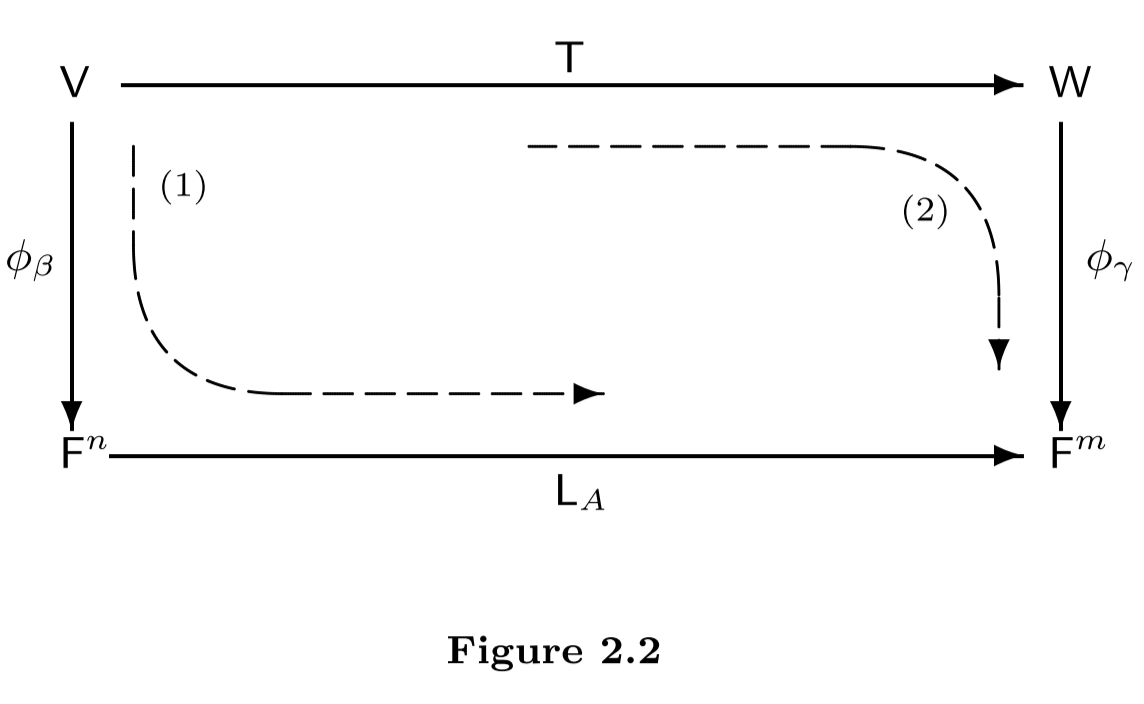
\includegraphics[width=16cm]{images/figure-2-2.png}

Let us first consider Figure 2.2.
Notice that there are two \emph{composites} of \LTRAN{}s that map \(\V\) into \(F^m\):
\begin{enumerate}
\item[1.] Map \(\V\) into \(F^n\) with \(\phi_{\beta}\) and follow this transformation with \(\LMTRAN_A\);
    this yields the composite \(\LMTRAN_A \phi_{\beta}\).
\item[2.] Map \(\V\) into \(\W\) with \(\T\) and follow it by \(\phi_{\gamma}\) to obtain the composite \(\phi_{\gamma} \T\).
\end{enumerate}

\begin{remark} \label{remark 2.4.6}
These two composites are depicted by the dashed arrows in the diagram.
By a simple reformulation of \THM{2.14}, we may conclude that for all \(v \in \V\),
\begin{align*}
    \LMTRAN_A \phi_{\beta}(v)
    & = \LMTRAN_A (\phi_{\beta}(v)) & \text{by def of composition} \\
    & = \LMTRAN_A([v]_{\beta}) & \text{by def of \(\phi_{\beta}\)} \\
    & = A [v]_{\beta} & \text{by def of \(\LMTRAN_A\)} \\
    & = [\T]_{\beta}^{\gamma} [v]_{\beta} & \text{since \(A = [\T]_{\beta}^{\gamma}\)} \\
    & = [\T(v)]_{\gamma} & \text{by \THM{2.14}} \\
    & = \phi_{\gamma}(\T(v)) & \text{by def of \(\phi_{\gamma}\)} \\
    & = \phi_{\gamma} \T (v), & \text{by def of composition}
\end{align*}

Hence \(\LMTRAN_A \phi_{\beta} = \phi_{\gamma} \T\);
that is. the diagram ``commutes.'' (It seems that the terminology is from abstract algebra.)

Heuristically, this relationship indicates that after \(\V\) and \(\W\) are \emph{identified} with \(F^n\) and \(F^m\) via if \(\phi_{\beta}\) and \(\phi_{\gamma}\), respectively,
we may ``identify'' \(\T\) with \(\LMTRAN_A\).
\textbf{This diagram allows us to transfer operations on abstract vector spaces to ones on \(F^n\) and \(F^m\)}.
\end{remark}

\begin{example} \label{example 2.4.7}
Recall the \LTRAN{} \(\T : \POLYRRR \to \POLYRR\) defined in \EXAMPLE{2.2.4} (\(\T(f(x)) = f'(x)\)).
Let \(\beta\) and \(\gamma\) be the standard ordered bases for \(\POLYRRR\) and \(\POLYRR\), respectively,
and let \(\phi_{\beta} : \POLYRRR \to \SET{R}^4\) and \(\phi_{\gamma} : \POLYRR \to \SET{R}^3\) be the corresponding standard representations of \(\POLYRRR\) and \(\POLYRR\).
If \(A = [\T]_{\beta}^{\gamma}\), then
\[
    A = \begin{pmatrix} 0 & 1 & 0 & 0 \\ 0 & 0 & 2 & 0 \\ 0 & 0 & 0 & 3 \end{pmatrix}
\]
Consider the polynomial \(p(x) = 2 + x - 3x^2 + 5x^3\).
We show that \(\LMTRAN_A \phi_{\beta} (p(x)) = \phi_{\gamma} \T (p(x))\).
Now
\[
    \LMTRAN_A \phi_{\beta} (p(x)) = [A]_{\beta}^{\gamma} [p(x)]_{\beta} 
    = \begin{pmatrix} 0 & 1 & 0 & 0 \\ 0 & 0 & 2 & 0 \\ 0 & 0 & 0 & 3 \end{pmatrix} \begin{pmatrix} 2 \\ 1 \\ -3 \\ 5 \end{pmatrix} = \begin{pmatrix} 1 \\ -6 \\ 15 \end{pmatrix}
\]
And since \(\T(p(x)) = p'(x) = 1 - 6x + 15x^2\), we have
\[
    \phi_{\gamma} \T (p(x)) = \phi_{\gamma} (1 - 6x + 15 x^2) = \begin{pmatrix} 1 \\ -6 \\ 15 \end{pmatrix}
\]
So \(\LMTRAN_A \phi_{\beta} (p(x)) = \phi_{\gamma} \T (p(x))\).
\end{example}

\exercisesection

\begin{exercise} \label{exercise 2.4.1}
Label the following statements as true or false.
In each part, \(V\) and \(W\) are vector spaces with ordered (finite) bases \(\alpha\) and \(\beta\), respectively, \(\T: V \to W\) is linear, and \(A\) and \(B\) are matrices.
\begin{enumerate}
\item \(([\T]_{\alpha}^{\beta})^{-1} = [\T^{-1}]_{\alpha}^{\beta}\).
\item \(\T\) is invertible if and only if \(\T\) is one-to-one and onto.
\item \(\T = \LMTRAN_A\), where \(A = [\T]_{\alpha}^{\beta}\).
\item \(M_{2 \X 3}(F)\) is isomorphic to \(F^5\).
\item \(\POLYNF\) is isomorphic to \(\mathcal{P}_m(F)\) if and only if \(n = m\).
\item \(AB = I\) implies that \(A\) and \(B\) are invertible.
\item If \(A\) is invertible, then \((A^{-1})^{-1} = A\).
\item \(A\) is invertible if and only if \(\LMTRAN_A\) is invertible.
\item \(A\) must be square in order to possess an inverse.
\end{enumerate}
\end{exercise}

\begin{proof} \ 

\begin{enumerate}
\item False.
    First, \(\T\) should be invertible to make \(\T^{-1}\) and \(([\T]_{\alpha}^{\beta})^{-1}\) well defined.
    Second, if \(\T\) is invertible, then by \THM{2.18}, \(([\T]_{\alpha}^{\beta})^{-1} = [\T^{-1}]_{\beta}^{\alpha}\).
\item True, this is just true for normal functions.
\item False. the domain and codomain of \(\T\) and \(\LMTRAN_A\) are not necessarily the same.
\item False, \(\dim(M_{2 \X 3}(F)) = 6 \ne 5 = \dim(F^5)\), so by \THM{2.19}, they are not isomorphic to each other.
\item True, \(\POLYNF\) is isomorphic to \(\mathcal{P}_m(F)\), if and only if (by \THM{2.19}) their dimension are equal, that is, if and only if \(n = m\).
\item False, by \DEF{2.13} we also need to check \(BA = I\); and \(A, B\) \emph{must be squares of the same size}.
    Counter example:
    \[
        \left(\begin{array}{lll}
            1 & 0 & 0 \\
            0 & 1 & 0
        \end{array}\right)
        \left(\begin{array}{ll}
            1 & 0 \\
            0 & 1 \\
            0 & 0
        \end{array}\right) = I_2
    \]
\item True.
    If \(A\) is invertible, then by \DEF{2.13}(3) we denote its inverse as \(A^{-1}\);
    in particular by \DEF{2.13}(1) we have \(A A^{-1} = A^{-1} A = I\).
    But this immediately implies \(A^{-1} A = A A^{-1} = I\), so by \DEF{2.13}(1) again, the (unique) inverse of \(A^{-1}\) is \(A\), that is, \((A^{-1})^{-1} = A\).
\item True by \CORO{2.18.2}.
\item True, by \DEF{2.13} (We only define ``invertible'' on square matrix'').
\end{enumerate}
\end{proof}

\begin{exercise} \label{exercise 2.4.2}
For each of the following linear transformations \(\T\), determine whether \(\T\) is invertible and justify your answer.
\begin{enumerate}
\item \(\T : \SET{R}^2 \to \SET{R}^3\) defined by \(\T(a_1, a_2) = (a_1 - 2a_2, a_2, 3a_1 + 4a_2)\).
\item \(\T : \SET{R}^2 \to \SET{R}^3\) defined by \(\T(a_1, a_2) = (3a_1 - a_2, a_2, 4a_1)\).
\item \(\T : \SET{R}^3 \to \SET{R}^3\) defined by \(\T(a_1, a_2, a_3) = (3a_1 - 2a_3, a_2, 3a_1 + 4a_2)\).
\item \(\T : \POLYRRR \to \POLYRR\) defined by \(\T(p(x)) = p'(x)\).
\item \(\T: M_{2 \X 2}(\SET{R}) \to \POLYRR\) defined by \(\T \begin{pmatrix} a & b \\ c & d \end{pmatrix} = a + 2bx + (c + d)x^2\).
\item \(\T : M_{2 \X 2}(\SET{R}) \to M_{2 \X 2}(\SET{R})\) defined by \(\T \begin{pmatrix} a & b \\ c & d \end{pmatrix} = \begin{pmatrix} a + b & a \\ c & c + d \end{pmatrix}\).
\end{enumerate}
\end{exercise}

\begin{proof} \ 

\begin{enumerate}
\item \(\T\) is not invertible since it cannot be an isomorphism by \THM{2.19}.
\item \(\T\) is not invertible since it cannot be an isomorphism by \THM{2.19}.
\item True.
    It's easy to check \(\NULLT = \{ (0, 0, 0) \}\), hence (by \THM{2.4}) \(\T\) is one-to-one (and by \THM{2.5}) is onto;
    and of course \(\T\) is linear, hence (by \RMK{2.4.1}) is invertible.
\item \(\T\) is not invertible since it cannot be an isomorphism by \THM{2.19}.
\item \(\T\) is not invertible since it cannot be an isomorphism by \THM{2.19}.
\item \(\T\) is invertible;
    It's easy to check \(\NULLT = \bigg\{ \begin{pmatrix} 0 & 0 \\ 0 & 0 \end{pmatrix} \bigg\}\), hence \(\T\) is one-to-one, and onto by \THM{2.5};
    and of course \(\T\) is linear.
\end{enumerate}
\end{proof}

\begin{exercise} \label{exercise 2.4.3}
Which of the following pairs of vector spaces are isomorphic?
Justify your answers.
\begin{enumerate}
\item \(F^3\) and \(\mathcal{P}_3(F)\).
\item \(F^4\) and \(\mathcal{P}_3(F)\).
\item \(M_{2 \X 2}(\SET{R})\) and \(\POLYRRR\).
\item \(V = \{ A \in M_{2 \X 2}(\SET{R}) : \TRACE(A) = 0 \}\) and \(\SET{R}^4\).
\end{enumerate}
\end{exercise}

\begin{proof} \ 
\begin{enumerate}
\item \(\dim(F^3) = 3\), \(\dim(\mathcal{P}_3(F)) = 4\), so \(F^3\) and \(\mathcal{P}_3(F)\) are not isomorphic by \THM{2.19}.
\item \(\dim(F^4) = 4\), \(\dim(\mathcal{P}_3(F)) = 4\), so \(F^4\) and \(\mathcal{P}_3(F)\) are isomorphic by \THM{2.19}.
\item \(\dim(M_{2 \X 2}(\SET{R})) = 4\), \(\dim(\mathcal{P}_3(F)) = 4\), so \(M_{2 \X 2}(\SET{R})\) and \(\mathcal{P}_3(F)\) are isomorphic by \THM{2.19}.
\item \(\dim(V) = 2^2 - 1 = 3\) by \ATHM{1.19}(1), \(\dim(\SET{R}^4) = 4\), so \(V\) and \(\SET{R}^4\) are not isomorphic by \THM{2.19}.
\end{enumerate}
\end{proof}

\begin{exercise} \label{exercise 2.4.4}
Let \(A\) and \(B\) be \(n \X n\) invertible matrices.
Prove that \(AB\) is invertible and \((AB)^{-1} = B^{-1}A^{-1}\).
\end{exercise}

\begin{proof}
We have
\begin{align*}
    (AB)(B^{-1}A^{-1}) & = ( A(B B^{-1}) )A^{-1} & \text{by \THM{2.16}, associative} \\
                       & = (A I_n) A^{-1} \\
                       & = A A^{-1} & \text{by \THM{2.12}(c)} \\
                       & = I_n,
\end{align*}
and
\begin{align*}
    (B^{-1}A^{-1})(AB) & = ( B(A A^{-1}) )B^{-1} & \text{by \THM{2.16}, associative} \\
                       & = (B I_n) B^{-1} \\
                       & = B B^{-1} & \text{by \THM{2.12}(c)} \\
                       & = I_n,
\end{align*}
so by \DEF{2.13}, \(AB\) is invertible, and (since the inverse is unique,) \((AB)^{-1} = B^{-1} A^{-1}\).
\end{proof}

\begin{exercise} \label{exercise 2.4.5}
Let \(A\) be invertible.
Prove that \(A^\top\) is invertible and \((A^\top)^{-1} = (A^{-1})^\top\).
\end{exercise}

\begin{note}
The inverse of the transpose of \(A\) is equal to the transpose of the inverse of \(A\), when \(A\) is invertible.
\end{note}

\begin{proof}
We have
\begin{align*}
    A^\top (A^{-1})^\top & = ( A^{-1} A )^\top & \text{by \ATHM{2.24}} \\
                       & = I_n^\top \\
                       & = I_n, & \text{of course}
\end{align*}
and
\begin{align*}
    (A^{-1})^\top A^\top  & = ( A A^{-1} )^\top & \text{by \ATHM{2.24}} \\
                       & = I_n^\top \\
                       & = I_n, & \text{of course}
\end{align*}
so by \DEF{2.13}, \(A^\top\) is invertible, and (since the inverse is unique,) \((A^\top)^{-1} = (A^{-1})^\top\).
\end{proof}

\begin{exercise} \label{exercise 2.4.6}
Prove that if \(A\) is \textbf{invertible} and \(AB = O\), then \(B = O\).
\end{exercise}

\begin{proof}
We have
\begin{align*}
             & AB = O \\
    \implies & A^{-1}(AB) = A^{-1} O = O \\
    \implies & (A^{-1} A)B = O & \text{by \THM{2.16}, associative} \\
    \implies & IB = O \\
    \implies & B = O. & \text{by \THM{2.12}(c)}
\end{align*}
\end{proof}

\begin{exercise} \label{exercise 2.4.7}
Let \(A\) be an \(n \X n\) matrix.
\begin{enumerate}
\item Suppose that \(A^2 = O_{n \X n}\).
    Prove that \(A\) is not invertible.
\item Suppose that \(AB = O_{n \X n}\) for some \textbf{nonzero} \(n \X n\) matrix \(B\).
    Could \(A\) be invertible? Explain.
\end{enumerate}
\end{exercise}

\begin{proof} \ 
\begin{enumerate}
\item For the sake of contradiction, suppose \(A\) is invertible (so we have \(A^{-1}\)).
Then
\begin{align*}
             & A^2 = O_{n \X n} \\
    \implies & A^{-1} (A^2) = A^{-1} O_{n \X n} = O_{n \X n} \\
    \implies & (A^{-1} A) A = O_{n \X n} & \text{by \THM{2.16}, associative} \\
    \implies & IA = O_{n \X n} \\
    \implies & A = O_{n \X n}, & \text{by \THM{2.13}(c)}
\end{align*}
which implies \(A\) is equal to a matrix that is not invertible, a contradiction.
Hence \(A\) is not invertible.

\item
If \(A\) is invertible, then
\begin{align*}
             & AB = O_{n \X n} \\
    \implies & A^{-1} (AB) = A O_{n \X n} = O_{n \X n} \\
    \implies & (A^{-1} A)B = O_{n \X n} & \text{by \THM{2.16}, associative} \\
    \implies & IB = O_{n \X n} \\
    \implies & B = O_{n \X n}, & \text{by \THM{2.13}(c)}
\end{align*}
which contradicts that \(B\) is nonzero.
Hence \(A\) is not invertible.
\end{enumerate}
\end{proof}

\begin{exercise} \label{exercise 2.4.8}
Prove \CORO{2.18.1} and \CORO{2.18.2}.
\end{exercise}

\begin{proof}
See \CORO{2.18.1} and \CORO{2.18.2}.
\end{proof}

\begin{exercise} \label{exercise 2.4.9}
Let \(A\) and \(B\) be \(n \X n\) matrices such that \(AB\) is invertible.
\begin{enumerate}
\item Prove that (\textbf{both}) \(A\) and \(B\) are invertible.
    Hint: See \ATHM{2.26}.
\item Give an example to show that a product of \emph{nonsquare} matrices can be invertible even though the factors, by definition, are not.
\end{enumerate}
\end{exercise}

\begin{note}
By part(b), the supposition that both \(A\) and \(B\) are \(n \X n\) matrix are essential to conclude that they are invertible.
\end{note}

\begin{proof}
Let \(\beta\) be the standard ordered basis for \(F^n\).
Then by \THM{2.15}(a), \([\LMTRAN_A]_{\beta} = A\), \([\LMTRAN_B]_{\beta} = B\), \([\LMTRAN_{AB}]_{\beta} = AB\),
and of course \(\LMTRAN_A, \LMTRAN_B, \LMTRAN_{AB}\) are linear.
\begin{enumerate}
\item Since \(AB\) is invertible, that is, \([\LMTRAN_{AB}]_{\beta}\) is invertible, by \THM{2.18}, \(\LMTRAN_{AB}\) is invertible, that is, by \THM{2.15}(e), \(\LMTRAN_A \LMTRAN_B\) is invertible.
By \ATHM{2.26}(1), \(\LMTRAN_B\) is one-to-one, and by \THM{2.5} (since domain/codomain have the same \(\dim\)), \(\LMTRAN_B\) is onto,
hence \(\LMTRAN_B\) is invertible, hence by \THM{2.18}, \([\LMTRAN_B]_{\beta}\) is invertible, that is, \(B\) is invertible.
Similarly, by \ATHM{2.26}(2), \(\LMTRAN_A\) is onto, and by \THM{2.5} (since domain/codomain have the same \(\dim\)), \(\LMTRAN_A\) is one-to-one,
hence \(\LMTRAN_A\) is invertible, hence by \THM{2.18}, \([\LMTRAN_A]_{\beta}\) is invertible, that is, \(A\) is invertible.

\item
We have
\begin{align*}
    \begin{pmatrix} 1 & 2 & 3 \end{pmatrix}
    \begin{pmatrix} 1 \\ 2 \\ 3 \end{pmatrix}
    = \begin{pmatrix} 10 \end{pmatrix},
\end{align*}
which is an \(1 \X 1\) matrix and has inverse \(( \frac{1}{10} )\).
\end{enumerate}
\end{proof}

\begin{exercise} \label{exercise 2.4.10}
Let \(A\) and \(B\) be \(n \X n\) matrices such that \(AB = I_n\).
\begin{enumerate}
\item Use \EXEC{2.4.9} to conclude that (\textbf{both}) \(A\) and \(B\) are invertible.
\item Prove \(A = B^{-1}\) (and hence \(B = A^{-1}\)).
    (We are, in effect, \textbf{saying that for square matrices, a "one-sided" inverse is a "two-sided" inverse.})
\item State and prove analogous results for linear transformations defined on finite-dimensional vector spaces.
\end{enumerate}
\end{exercise}

\begin{note}
Part(b) says, if \(A, B\) are squares and \(AB = I_n\), then we automatically have \(BA = I_n\), and \(A, B\) are inverse matrices of each other.
\end{note}

\begin{proof} \ 
\begin{enumerate}
\item If \(AB = I_n\), that simply means \(AB\) is invertible, since \(I_n\) is invertible.
So the conditions of \EXEC{2.4.9}(a) are satisfied, hence both \(A, B\) are invertible.

\item We have
\begin{align*}
             & AB = I_n \\
    \implies & A^{-1} (AB) = A^{-1} I_n = A^{-1} & \text{since \(A\) is invertible, and by \THM{2.12}(c)} \\
    \implies & (A^{-1}A)B = A^{-1} & \text{by \THM{2.16}, associative} \\
    \implies & I_n B = A^{-1} \\
    \implies & B = A^{-1}. & \text{by \THM{2.12}(c)}
\end{align*}
And by \DEF{2.13}, this implies \(AB = BA = I_n\).
In particular, we have \(BA = AB = I_n\), so by \DEF{2.13} again, \(B^{-1} = A\).

\item
Statement: Let \(\T : V \to W\) and \(\U : W \to V\) where \(V, W\) have same (finite) dimensions and \(\U\T = \ITRANV\).
Then both \(\U, \T\) are invertible. and we have \((\T)^{-1} = \U\) (hence \(\U^{-1} = \T\)).

First, similar to \EXEC{2.4.9}, by \ATHM{2.26}(1)(2), both \(\U, \T\) are invertible.
And (by general version of \THM{2.10},) we have
\begin{align*}
             & \U\T = \ITRANV \\
    \implies & \U^{-1} (\U\T) = \U^{-1} \ITRANV = \U^{-1} & \text{since \(\U\) is invertible, and by \THM{2.10}(c)} \\
    \implies & (\U^{-1}\U)\T = \U^{-1} & \text{by \THM{2.10}(b), associative} \\
    \implies & \ITRANW \T = \U^{-1} \\
    \implies & \T = \U^{-1}. & \text{by \THM{2.10}(c)}
\end{align*}
And by \DEF{2.12}, this implies \(\U\T = \ITRANV\) and \(\T\U = \ITRANW\).
In particular, we have \(\T\U = \ITRANW\) and \(\U\T = \ITRANV\) and, so by \DEF{2.12} again, \(\T^{-1} = \U\).
\end{enumerate}
\end{proof}

\begin{exercise} \label{exercise 2.4.11}
Verify that the transformation in \EXAMPLE{2.4.5} is one-to-one.
\end{exercise}

\begin{proof}
Suppose \(f \in \NULLT\), we have to show \(f\) is zero polynomial to show \(\T\) is one-to-one.
Then we have \(f(1) = f(2) = f(3) = f(4) = 0\).
But by \RMK{1.6.6} we know that \(f\) is the zero polynomial, as desired.
\end{proof}

\begin{exercise} \label{exercise 2.4.12}
Prove \THM{2.21}.
\end{exercise}

\begin{proof}
See \THM{2.21}.
\end{proof}

\begin{exercise} \label{exercise 2.4.13}
Let \(\sim\) mean ``is isomorphic to.'' (\DEF{2.14})
Prove that \(\sim\) is an equivalence relation on the class of vector spaces over \(F\).
\end{exercise}

\begin{proof}\ 

Reflexivity: \(V\) is isomorphic to \(V\) since \(\ITRANV\) is an isomorphism from \(V\) to \(V\) for any vector space \(V\).

Symmetry: Suppose \(V\) is isomorphic to \(W\), then there exists an isomorphism \(\T\) from \(V\) to \(W\).
In particular, by \DEF{2.14}, \(\T\) is invertible, so \(\T^{-1} : W \to V\) exists, and also invertible.
And by \THM{2.17}, \(\T^{-1}\) is linear.
Hence by \DEF{2.14} again, \(\T^{-1}\) is an isomorphism from \(W\) to \(V\).
Hence \(W\) is isomorphic to \(V\).

Transitivity: Suppose \(V\) is isomorphic to \(W\) and \(W\) is isomorphic to \(Z\), then there exists an isomorphism \(\T\) from \(V\) to \(W\) and \(\U\) from \(W\) to \(Z\).
Furthermore, by \ATHM{2.26}(c) \(\U\T\) is invertible, and by \THM{2.9}, since \(\U, \T\) are linear, \(\U\T\) is also linear, hence \(\U\T\) is an isomorphism by \DEF{2.14}.
Hence \(V\) is isomorphic to \(Z\).
\end{proof}

\begin{exercise} \label{exercise 2.4.14}
Let
\[
    V = \bigg\{ \begin{pmatrix} a & a + b \\ 0 & c \end{pmatrix} : a, b, c \in F \bigg\}.
\]
Construct an isomorphism from \(V\) to \(F^3\).
\end{exercise}

\begin{proof}
Clearly,
\[\beta = \bigg\{
    \begin{pmatrix} 1 & 0 \\ 0 & 0 \end{pmatrix},
    \begin{pmatrix} 0 & 1 \\ 0 & 0 \end{pmatrix},
    \begin{pmatrix} 0 & 0 \\ 0 & 1 \end{pmatrix}
\bigg\}\]
is a basis for \(V\).
Then by \THM{2.21}, \(\phi_{\beta}\) is an isomorphism from \(V\) to \(F^3\).
\end{proof}

\begin{exercise} \label{exercise 2.4.15}
Let \(V\) and \(W\) be \(n\)-dimensional vector spaces, and let \(\T : V \to W\) be a linear transformation.
Suppose that \(\beta\) is a basis for \(V\).
Prove that \(\T\) is an isomorphism \emph{if and only if} \(\T(\beta)\) is a basis for \(W\).
\end{exercise}

\begin{proof} \ 

\(\Longrightarrow\): Suppose \(\T\) is an isomorphism.
In particular, \(\T\) is one-to-one and onto.
Then by \ATHM{2.2}(2.c), \(\T(\beta)\) is a basis for \(W\).

\(\Longleftarrow\): Suppose \(\T(\beta)\) is a basis for \(W\).
In particular, \(\spann(\T(\beta)) = W\).
And by \THM{2.2}, \(\RANGET = \spann(\T(\beta)) = W\), hence \(\T\) is onto.
By \THM{2.5}, \(\T\) is one-to-one.
Hence \(\T\) is an isomorphism.
\end{proof}

\begin{exercise} \label{exercise 2.4.16}
Let \(B\) be an \(n \X n\) \emph{invertible} matrix.
Define \(\Phi : M_{n \X n}(F) \to M_{n \X n}(F)\) by \(\Phi(A) = B^{-1}AB\).
Prove that \(\Phi\) is an isomorphism.
\end{exercise}

\begin{note}
This is called ``matrix similarity''; we say that \(\Phi(A)\)(or \(B^{-1}AB\)) and \(A\) are similar.
This concept is introduced in the next section(\DEF{2.16}) and is used in \CH{5}.
\end{note}

\begin{proof}
First, it's trivial that \(\Phi\) is linear since it only involves matrix multiplication and you can use \THM{2.10} to check linearity.
Now to show that \(\Phi\) is invertible, since domain/codomain have the same dimensions, we only need to show \(\Phi\) is onto.
But given \(D \in M_{n \X n}(F)\), we have \(B D B^{-1} \in M_{n \X n}(F)\) such that
\begin{align*}
    \Phi(B D B^{-1}) & = B^{-1} (B D B^{-1}) B & \text{by def of \(\Phi\)} \\
                     & = (B^{-1}B) D (B^{-1} B) & \text{of course} \\
                     & = IDI & \text{of course} \\
                     & = D & \text{of course}
\end{align*}
So \(\Phi\) is onto, as desired.
\end{proof}

\begin{exercise} \label{exercise 2.4.17}
Let \(V\) and \(W\) be finite-dimensional vector spaces and \(\T : V \to W\) be an isomorphism.
Let \(V_0\) be a \emph{subspace} of \(V\).
\begin{enumerate}
\item Prove that \(\T(V_0)\) is a subspace of \(W\).
\item Prove that \(\dim(V_0) = \dim(\T(V_0))\).
\end{enumerate}
And from part(b), we say that an isomorphism is \emph{rank-preserving}, since in particular \(\dim(V) = \dim(\T(V))\).
\end{exercise}

\begin{proof} \ 

\begin{enumerate}
\item It is true by \ATHM{2.4}(1).
\item By \THM{2.19}, it suffices to show that \(V_0\) and \(\T(V_0)\) are isomorphic.
And we claim that \(\T' : V_0 \to \T(V_0)\) by \(\T'(v) = \T(v)\) for \(v \in V_0\) is an isomorphism from \(V_0\) to \(\T(V_0)\).

First, of course \(\T'\) is linear.
For one-to-one, given \(v_1, v_2 \in V_0\),
\begin{align*}
             & \T'(v_1) = \T'(v_2) \\
    \implies & \T(v_1) = \T(v_2) & \text{by def of \(\T'\)} \\
    \implies & v_1 = v_2. & \text{since in particular \(\T\) is one-to-one}
\end{align*}

For onto, given \(w \in \T(V_0)\), then by definition of \(\T(V_0)\) we of course can find \(v \in V_0\) such that \(\T(v) = W\).
But since \(v \in V_0\), \(\T'(v) = \T(v)\).
Hence we have found \(v \in V_0\) such that \(\T'(v) = w\), so \(\T'\) is onto.

So \(\T'\) is an isomorphism from \(V_0\) to \(\T(V_0)\), as desired.
\end{enumerate}

\end{proof}

\begin{exercise} \label{exercise 2.4.18}
Repeat \EXAMPLE{2.4.7} with the polynomial \(p(x) = 1 + x + 2x^2 + x^3\).
\end{exercise}

\begin{proof}
Let 
\[
    A = [\T]_{\beta}^{\gamma} = \begin{pmatrix} 0 & 1 & 0 & 0 \\ 0 & 0 & 2 & 0 \\ 0 & 0 & 0 & 3 \end{pmatrix}
\]
We show that \(\LMTRAN_A \phi_{\beta} (p(x)) = \phi_{\gamma} \T (p(x))\).
Now
\[
    \LMTRAN_A \phi_{\beta} (p(x)) = [A]_{\beta}^{\gamma} [p(x)]_{\beta} 
    = \begin{pmatrix} 0 & 1 & 0 & 0 \\ 0 & 0 & 2 & 0 \\ 0 & 0 & 0 & 3 \end{pmatrix} \begin{pmatrix} 1 \\ 1 \\ 2 \\ 1 \end{pmatrix} = \begin{pmatrix} 1 \\ 4 \\ 3 \end{pmatrix}
\]
But since \(\T(p(x)) = p'(x) = 1 + 4x + 3x^2\), we have
\[
    \phi_{\gamma} \T (p(x)) = \phi_{\gamma} (1 + 4x + 3x^2) = \begin{pmatrix} 1 \\ 4 \\ 3 \end{pmatrix}
\]
So \(\LMTRAN_A \phi_{\beta} (p(x)) = \phi_{\gamma} \T (p(x))\).
\end{proof}

\begin{exercise} \label{exercise 2.4.19}
In \EXAMPLE{2.1.5}, the mapping \(\T : M_{2 \X 2}(\SET{R}) \to M_{2 \X 2}(\SET{R})\) defined by \(\T(M) = M^\top\) for each \(M \in M_{2 \X 2}(\SET{R})\) is a linear transformation.
Let \(\beta = \{ E_{11}, E_{12}, E_{21}, E_{22} \}\), which is a basis for \(M_{2 \X 2}(\SET{R})\), as noted in \EXAMPLE{1.6.3}.
\begin{enumerate}
\item Compute \([\T]_{\beta}\).
\item Verify that \(\LMTRAN_A \phi_{\beta} (M) = \phi_{\beta} \T(M)\) for \(A = [\T]_{\beta}\) and \(M = \begin{pmatrix} 1 & 2 \\ 3 & 4 \end{pmatrix}\).
\end{enumerate}
\end{exercise}

\begin{proof} \ 

\begin{enumerate}
\item From \EXEC{2.2.5}(a),
\[
    [\T]_{\beta}
    = \begin{pmatrix}
        \MAROON{1} & \BLUE{0} & \RED{0} & \GREEN{0} \\
        \MAROON{0} & \BLUE{0} & \RED{1} & \GREEN{0} \\
        \MAROON{0} & \BLUE{1} & \RED{0} & \GREEN{0} \\
        \MAROON{0} & \BLUE{0} & \RED{0} & \GREEN{1}
    \end{pmatrix}
\]

\item
\[
    \LMTRAN_A \phi_{\beta}(M) = 
    = \begin{pmatrix}
        1 & 0 & 0 & 0 \\
        0 & 0 & 1 & 0 \\
        0 & 1 & 0 & 1 \\
        0 & 0 & 0 & 1
    \end{pmatrix}
    \begin{pmatrix} 1 \\ 2 \\ 3 \\4 \end{pmatrix}
    = \begin{pmatrix} 1 \\ 3 \\ 2 \\ 4 \end{pmatrix}
\]
and
\[
    \phi_{\beta}\T(M)
    = \phi_{\beta}\begin{pmatrix} 1 & 3 \\ 2 & 4 \end{pmatrix}
    = \begin{pmatrix} 1 \\ 3 \\ 2 \\ 4 \end{pmatrix}
\]
So \(\LMTRAN_A \phi_{\beta}(M) = \phi_{\beta}\T(M)\).
\end{enumerate}
\end{proof}

\begin{exercise} \label{exercise 2.4.20}
Let \(\T: V \to W\) be a \LTRAN{} from an \(n\)-dimensional vector space \(V\) to an \(m\)-dimensional vector space \(W\).
Let \(\beta\) and \(\gamma\) be ordered bases for \(V\) and \(W\), respectively.
Prove that \(\rankT = \rank(\LMTRAN_A)\) and that \(\nullityT = \nullity(\LMTRAN_A)\), where \(A = [\T]_{\beta}^{\gamma}\).
Hint: Apply \EXEC{2.4.17} to Figure 2.2.
\end{exercise}

\begin{proof} \ 

\(\rankT = \rank(\LMTRAN_A)\):
Since \(\LMTRAN_A \phi_{\beta} = \phi_{\gamma} \T \), in particular we have \(\LMTRAN_A \phi_{\beta}(V) = \phi_{\gamma} \T(V)\) \MAROON{(1)}.

Now, for the dimension of RHS of \MAROON{(1)},
\begin{align*}
    & \dim(\phi_{\gamma} \T(V)) \\
    & = \dim(\phi_{\gamma} (\T(V))) & \text{by def of composition} \\
    & = \dim(\T(V)) & \text{since \(\phi_{\gamma}\) is an isomorphism, and by \EXEC{2.4.17}(b)} \\
    & = \rankT, & \text{by definition}
\end{align*}
and for the dimension of LHS of \MAROON{(1)},
\begin{align*}
    & \dim(\LMTRAN_A \phi_{\beta}(V)) \\
    & = \dim(\LMTRAN_A (\phi_{\beta}(V))) & \text{by def of composition} \\
    & = \dim(\LMTRAN_A (F^n)) & \text{since (in particular) \(\phi_{\beta}\) is onto} \\
    & = \dim(\RANGE(\LMTRAN_A)) & \text{by definition} \\
    & = \rank(\LMTRAN_A), & \text{by definition}
\end{align*}
Hence we have \(\rankT = \rank(\LMTRAN_A)\), as desired.

\(\nullityT = \nullity(\LMTRAN_A)\):
We have
\begin{align*}
    \nullityT & = \dim(V) - \rankT & \text{by \THM{2.3}(dimension theorem)} \\
              & = \dim(F^n) - \rankT & \text{of course, since \(\dim(V) = n\)} \\
              & = \dim(F^n) - \rank(\LMTRAN_A) & \text{by what we have shown} \\
              & = \nullity(\LMTRAN_A). & \text{again by \THM{2.3}}
\end{align*}
\end{proof}

\begin{exercise} \label{exercise 2.4.21}
Let \(V\) and \(W\) be \emph{finite}-dimensional vector spaces with ordered bases \(\beta = \{ v_1, v_2, ..., v_n \}\) and \(\gamma = \{ w_1, w_2, ..., w_m \}\), respectively.
By \THM{2.6}, there exist unique linear transformations \(\T_{ij} : V \to W\) such that
\begin{equation*}
    \T_{ij}(v_k) = \begin{cases}
        w_i, \text{ if } k = j \\
        \OW, \text{ if } k \ne j
    \end{cases}
\end{equation*}
First prove that \(\alpha = \{ T_{ij} : 1 \le i \le m, 1 \le j \le n \}\) is a basis for \(\mathcal{L}(V, W)\).
Then let \(M^{ij}\) be the \(m \X n\) matrix with \(1\) in the \(i\)th row and \(j\)th column and \(0\) elsewhere, and prove that \([\T_{ij}]_{\beta}^{\gamma} = M^{ij}\).
Again by \THM{2.6}, there exists a unique linear transformation \(\Phi_{\beta}^{\gamma} : \mathcal{L}(V, W) \to M_{m \X n}(F)\) such that \(\Phi_{\beta}^{\gamma} (\T_{ij}) = M^{ij}\).
Prove that \(\Phi_{\beta}^{\gamma}\) is an isomorphism.
\end{exercise}

\begin{proof}
Since \(\#\alpha = \dim(\mathcal{L}(V, W)\) (where by \THM{2.20} we can conclude \(\dim(\mathcal{L}(V, W) = mn\)), (by \CORO{1.10.3}(b)) we only need to show \(\alpha\) is \LID{}.
BTW, we use the symbol \(\TZERO\) to represent the zero vector, i.e. the zero transformation, of \(\mathcal{L}(V, W)\).

So suppose \(\sum_{i = 1}^{m} \sum_{j = 1}^n a_{ij} \T_{ij} = \TZERO\) \MAROON{(1)}, we have to show \(a_{ij} = 0\) for all \(1 \le i \le m\), \(1 \le j \le n\).
But given arbitrary \(k\) such that \(1 \le k \le n\),
\begin{align*}
    \OW & = \TZERO(v_k) & \text{of course} \\
        & = \bigg( \sum_{i = 1}^{m} \sum_{j = 1}^n a_{ij} \T_{ij} \bigg) (v_k) & \text{by \MAROON{(1)}} \\
        & = \sum_{i = 1}^{m} \sum_{j = 1}^n a_{ij} \T_{ij} (v_k) & \text{by def of \(+\) and scalar \(\cdot\) of functions} \\
        & = \sum_{i = 1}^{m} \bigg( a_{i1} \T_{i1} (v_k) + a_{i2} \T_{i2} (v_k) + ... + a_{in} \T_{in} (v_k) \bigg) & \text{expanding summation} \\
        & = \sum_{i = 1}^{m} \bigg( a_{i1} \OV + ... + a_{ik} w_i + ... + a_{in} \OV \bigg) & \text{by definition of \(\T_{ij}\)} \\
        & = \sum_{i = 1}^m a_{ik} w_i,
\end{align*}
which implies \(a_{1k} = a_{2k} = ... = a_{mk} = 0\) since \(\gamma\) is a basis for \(W\).
Since \(k\) is arbitrary, we have \(a_{ik} = 1\) for all \(1 \le i \le m\), \(1 \le k \le n\), as desired.

Now given arbitrary \(j\) such that \(1 \le j \le n\), it trivial that the \(j\)th column of \(M^{ij}\) is \(e_i\) where \(e_i\) is the \(i\)th standard vector of \(F^m\).
And by definition, the \(j\)th column of \([\T_{ij}]_{\beta}^{\gamma}\) is \([\T_{ij}(v_j)]_{\gamma}\), but
\begin{align*}
    [\T_{ij}(v_j)]_{\gamma} & = [w_i]_{\gamma} & \text{by definition of \(T^{ij}\)} \\
                 & = e_i & \text{of course}
\end{align*}
Hence \(M^{ij} = [\T_{ij}]_{\gamma}\).

Finally, And since \(\alpha' = \{ M_{ij} : 1 \le i \le m, 1 \le j \le n \}\) is a basis for \(M_{m \X n}(F)\), and \(\Phi_{\beta}^{\gamma}(\alpha) = \alpha'\), by \EXEC{2.4.15}, \(\Phi_{\beta}^{\gamma}\) is an isomorphism.
\end{proof}

\begin{exercise} \label{exercise 2.4.22}
Let \(c_0, c_1, ..., c_n\) be \emph{distinct} scalars from an infinite field \(F\).
Define \(\T: \POLYNF \to F^{n + 1}\) by \(\T(f) = (f(c_0), f(c_1), ..., f(c_n))\).
Prove that \(\T\) is an isomorphism.
Hint: Use the Lagrange polynomials associated with \(c_0, c_1, ..., c_n\).
\end{exercise}

\begin{proof}
(This exercise is similar to \EXEC{2.4.11}.)
First it's of course that \(\T\) is linear.
And since \(\dim(\POLYNF) = \dim(F^{n + 1})\), we only have to show \(\T\) is one-to-one.
So suppose \(f \in \NULLT\), we have to show \(f\) is zero polynomial to show \(\T\) is one-to-one.
Then we have \(\T(f) = (f(c_0), f(c_1), ..., f(c_n)) = (0, 0, ..., 0)\).
But by \RMK{1.6.6}, we know that \(f\) is zero polynomial, as desired.
\end{proof}

\begin{exercise} \label{exercise 2.4.23}
Let \(W\) denote the vector space of all \emph{sequences} in \(F\) that \emph{have only a finite number of nonzero terms} (defined in \EXEC{1.6.18}),
and let \(Z = \POLYF\).
Define
\[
    \T : W \to Z \text{ by } \T(\sigma) = \sum_{i = 0}^n \sigma(i)x^i,
\]
where \(n\) is the \emph{largest integer} such that \(\sigma(n) \ne 0\). Prove that \(\T\) is an isomorphism.
\end{exercise}

\begin{proof}
Since the domain and codomain of \(\T\) are infinite-dimensional, we need to show that \(\T\) is linear, one-to-one, onto, respectively.

First, given \(\sigma_1, \sigma_2 \in W\) and scalar \(c \in F\), where \(n_1\), \(n_2\) are the largest nonzero integers such that \(\sigma_1(n_1) \ne 0\) and \(\sigma_2(n_2) \ne 0\), respectively.
Then
\begin{align*}
    & \T(\sigma_1 + c \sigma_2) \\
    & = \sum_{i = 0}^{\max(n_1, n_2)} (\sigma_1 + c \sigma_2)(i) x^i & \text{by def of \(\T\)} \\
    & = \sum_{i = 0}^{\max(n_1, n_2)} (\sigma_1(i) + c \sigma_2(i)) x^i & \text{by def of \(+\) and scalar \(\cdot\) of functions} \\
    & = \sum_{i = 0}^{\max(n_1, n_2)} \sigma_1(i) x^i + c \sigma_2(i) x^i & \text{of course} \\
    & = \sum_{i = 0}^{\max(n_1, n_2)} \sigma_1(i) x^i + c \sum_{i = 0}^{\max(n_1, n_2)} \sigma_2(i) x^i & \text{by splitting summation and move constant} \\
    & = \sum_{i = 0}^{n_1} \sigma_1(i) x^i + c \sum_{i = 0}^{n_2} \sigma_2(i) x^i & \text{of course} \\
    & = \T(\sigma_1) + c\T(\sigma_2), & \text{by def of \(\T\)}
\end{align*}
hence by \ATHM{2.1}(b), \(\T\) is linear.

Now, by the property of polynomial, it's really clear that \(\T\) is one-to-one (only zero sequence gives zero polynomial) and onto (every polynomial can be represented as a sequence of finite nonzero terms), hence \(\T\) is an isomorphism.
\end{proof}

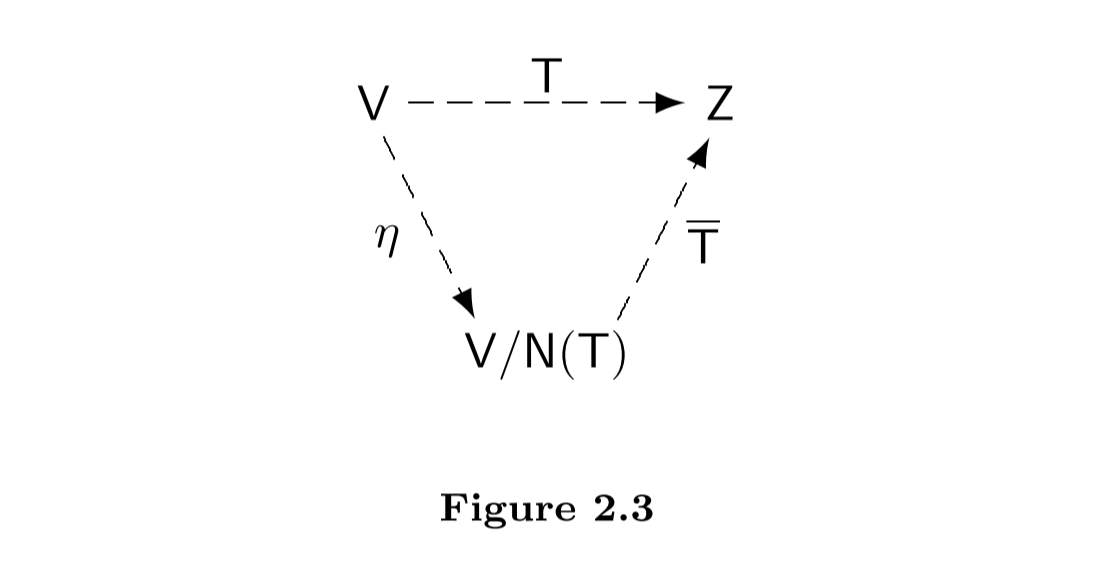
\includegraphics[width=16cm]{images/figure-2-3.png}

\begin{exercise} \label{exercise 2.4.24}
Let \(V\) and \(Z\) be vector spaces and \(\T : V \to Z\) be a linear transformation \emph{that is onto}.
Define the mapping
\[
    \overline{\T} : V / \NULLT \to Z \text{ by } \overline{\T}(v + \NULLT) = \T(v)
\]
for any coset \(v + \NULLT\) in \(V / \NULLT\).
\begin{enumerate}
\item Prove that \(\overline{\T}\) is \emph{well-defined};
    that is, prove that if \(v + \NULLT = v' + \NULLT\), then \(\T(v) = \T(v')\).
\item Prove that \(\overline{\T}\) is linear.
\item Prove that \(\overline{\T}\) is an isomorphism.
\item Prove that the diagram shown in Figure 2.3 \emph{commutes};
    that is, prove that \(\T = \overline{\T} \eta\). (\(\eta\) is defined in \EXEC{2.1.42}.)
\end{enumerate}

Note that we do not say \(V\) and \(Z\) are finite dimensional.
\end{exercise}

\begin{proof} \ 

\begin{enumerate}
\item Suppose \(v + \NULLT = v' + \NULLT\), then by \ATHM{1.10}(b), \(v - v' \in \NULLT\), which implies \(\T(v - v') = 0_{_Z}\), that is, \(\T(v) - \T(v') = 0_{_Z}\), that is, \(\T(v) = \T(v')\).

\item For any \(v_1 + \NULLT\) and \(v_2 + \NULLT\) in \(V/\NULLT\), and any scalar \(c\),
\begin{align*}
    & \overline{\T}\bigg( \big( v_1 + \NULLT \big) + c \big(v_2 + \NULLT \big)  \bigg) \\
    & = \overline{\T}\big( (v_1 + cv_2) + \NULLT) \big) & \text{by def of coset \(+\) and scalar \(\cdot\), see \EXEC{1.3.31}} \\
    & = \T(v_1 + cv_2) & \text{by def of \(\overline{\T}\)} \\
    & = \T(v_1) + c\T(v_2) & \text{since \(\T\) is linear} \\
    & = \overline{\T}(v_1 + \NULLT) + c\overline{\T}(v_2 + \NULLT), & \text{by def of \(\overline{\T}\)}
\end{align*}
hence by \ATHM{2.1}(b), \(\overline{\T}\) is linear.

\item Now we have to show \(\overline{\T}\) is one-to-one and onto.
For one-to-one, suppose \(v + \NULLT \in \NULL(\overline{\T})\), we have to show \(v + \NULLT = \OV + \NULLT\).
Then by definition of \(\overline{\T}\), \(\overline{\T}(v + \NULLT) = \T(v) = 0_{_Z}\), which implies \(v \in \NULLT\).
And of course \(v - \OV \in \NULLT\), so by \ATHM{1.10}(b), \(v + \NULLT = \OV + \NULLT\), as desired.

For onto, suppose arbitrary \(z \in Z\).
\emph{Then since \(\T\) is onto}, we can find \(v \in V\) such that \(\T(v) = z\), and for such \(v\) of course we can find \(v + \NULLT \in V/\NULLT\) such that \(\overline{\T}(v + \NULLT) = \T(v) = z\).
Hence \(\overline{\T}\) is onto.

Hence \(\overline{\T}\) is an isomorphism from \(V/\NULLT\) to \(Z\).

\item It's somewhat ambiguous that the exercise does not mention the corresponding \(W\) of the linear map \(\eta\).
Anyway, we assume \(\eta : V \to V/\NULLT\) by \(\eta(v) = v + \NULLT\).
Then for all \(v \in V\), we have
\begin{align*}
    \overline{\T}\eta(v) & = \overline{\T}(\eta(v)) & \text{by def of composition} \\
                         & = \overline{\T}(v + \NULLT) & \text{by def of \(\eta\)} \\
                         & = \T(v) & \text{by def of \(\overline{\T}\)}
\end{align*}
Hence \(\T = \overline{\T}\eta\).
\end{enumerate}
\end{proof}

\begin{exercise} \label{exercise 2.4.25}
\TODOREF{} \RED{Skip}, this need section 1.7.
\end{exercise}

\begin{proof}
\end{proof}

\begin{additional theorem} \label{athm 2.36}
This is the placeholder theorem for some matrix inversion equations:

\BLUE{(1)} \EXEC{2.4.4}: \((AB)^{-1} = B^{-1} A^{-1}\) when \(A, B\) are invertible (and compatible).

\BLUE{(2)} \EXEC{2.4.5}: \((A^\top)^{-1} = (A^{-1})^\top\) when \(A\) is invertible.
\end{additional theorem}

\begin{additional theorem} \label{athm 2.37}
This is the placeholder theorem for some judgement of zero matrix and invertibility:

\BLUE{(1)} \EXEC{2.4.6}: If \(A\) is invertible and \(AB = O\), then \(B = O\).

\EXEC{2.4.7}:

\BLUE{(2.1)}: If \(A^2 = O\) then \(A\) is not invertible.

\BLUE{(2.2)}: If \(AB = O\) for some \emph{nonzero} \(n \X n\) matrix \(B\), then \(A\) is not invertible.

\BLUE{(3)} \EXEC{2.4.9}: If \(A\) and \(B\) be \(n \X n\) matrices such that \(AB\) is invertible, then both \(A\) and \(B\) are invertible.
\end{additional theorem}

\begin{additional theorem} \label{athm 2.38}
This is the placeholder theorem for \EXEC{2.4.10}:

\BLUE{(1)}: If \(A, B\) are \(n \X n\) squares and \(AB = I_n\), then \(A, B\) are invertible, and \(A = B^{-1}\) and \(B = A^{-1}\).
In fact, we do not need to check \(BA = I_n\), hence a ``one-sided'' inverse is a ``two-sided'' inverse.

\BLUE{(2)}: Analogous result for \LTRAN{}:
Let \(\T : V \to W\) and \(\U : W \to V\) where \(V, W\) have same (finite) dimensions and \(\U\T = \ITRANV\).
Then both \(\U, \T\) are invertible. and we have \((\T)^{-1} = \U\) (hence \(\U^{-1} = \T\)).
\end{additional theorem}

\begin{additional theorem} \label{athm 2.39}
This is the placeholder theorem for \EXEC{2.4.15}:
If \(\T : V \to W\) is a \LTRAN{}, and \(\beta\) is a basis for \(V\), then \(\T\) is an isomorphism (from \(V\) to \(W\)) if and only if \(\T(\beta)\) is a basis for \(W\).
\end{additional theorem}

\begin{additional theorem} \label{athm 2.40}
This is the placeholder theorem for \EXEC{2.4.16}:
Given \(n \X n\) invertible matrix \(B\),
\(\Phi : M_{n \X n}(F) \to M_{n \X n}(F)\) by \(\Phi(A) = B^{-1}AB\) is an isomorphism.
\end{additional theorem}

\begin{additional theorem} \label{athm 2.41}
This is the placeholder theorem for \EXEC{2.4.17}:
Let \(V\) and \(W\) be finite-dimensional vector spaces and \(\T : V \to W\) be an isomorphism.
Let \(V_0\) be a \emph{subspace} of \(V\).
Then

\BLUE{(1)} \(\T(V_0)\) is a subspace of \(W\), and

\BLUE{(2)} \(\dim(V_0) = \dim(\T(V_0))\);
    we say that an isomorphism is \emph{rank-preserving}, since in particular \(\dim(V) = \dim(\T(V))\).
\end{additional theorem}

\begin{additional theorem} \label{athm 2.42}
This is the placeholder theorem for \EXEC{2.4.20}:
Let \(\T: V \to W\) be a linear transformation from an \(n\)-dimensional vector space \(V\) to an \(m\)-dimensional vector space \(W\).
Let \(\beta\) and \(\gamma\) be ordered bases for \(V\) and \(W\), respectively.
Then \(\rankT = \rank(\LMTRAN_A)\) and that \(\nullityT = \nullity(\LMTRAN_A)\), where \(A = [\T]_{\beta}^{\gamma}\).
\end{additional theorem}

\begin{additional theorem} \label{athm 2.43}
This is the placeholder theorem for \EXEC{2.4.21}, which gives an isomorphism \(\Phi_{\beta}^{\gamma} : \mathcal{L}(V, W) \to M_{m \X n}(F)\).
\end{additional theorem}

\begin{additional theorem} \label{athm 2.44}
This is the placeholder theorem for \EXEC{2.4.22}, which gives an isomorphism from \(\POLYNF\) to \(F^{n + 1}\);
And this isomorphism is related to Lagrange polynomials(or \RMK{1.6.6}).
\end{additional theorem}

\begin{additional theorem} \label{athm 2.45}
This is the placeholder theorem for \EXEC{2.4.24}, which gives some other facts about quotient space.
\end{additional theorem}
\section{The Change of Coordinate Matrix} \label{sec 2.5}

\begin{note}
Some of inverse matrices in the examples are (mysteriously) given, but in fact currently we do not know how to calculate the inverse of a invertible matrix.
This is introduced in \CH{3}.
\end{note}

In many areas of mathematics, a \emph{change of variable} is used to \emph{simplify the appearance} of an expression.
For example, in geometry the change of variable
\[
    \begin{array}{l}
        x=\frac{2}{\sqrt{5}} x^{\prime}-\frac{1}{\sqrt{5}} y^{\prime} \\
        y=\frac{1}{\sqrt{5}} x^{\prime}+\frac{2}{\sqrt{5}} y^{\prime}
\end{array}
\]
can be used to transform the equation \(2x^2 - 4xy + 5y^2 = 1\) into the simpler equation \((x')^2 + 6(y')^2 = 1\), a \emph{form} in which it is easily seen to be the equation of an ellipse. (See Figure 2.4.)

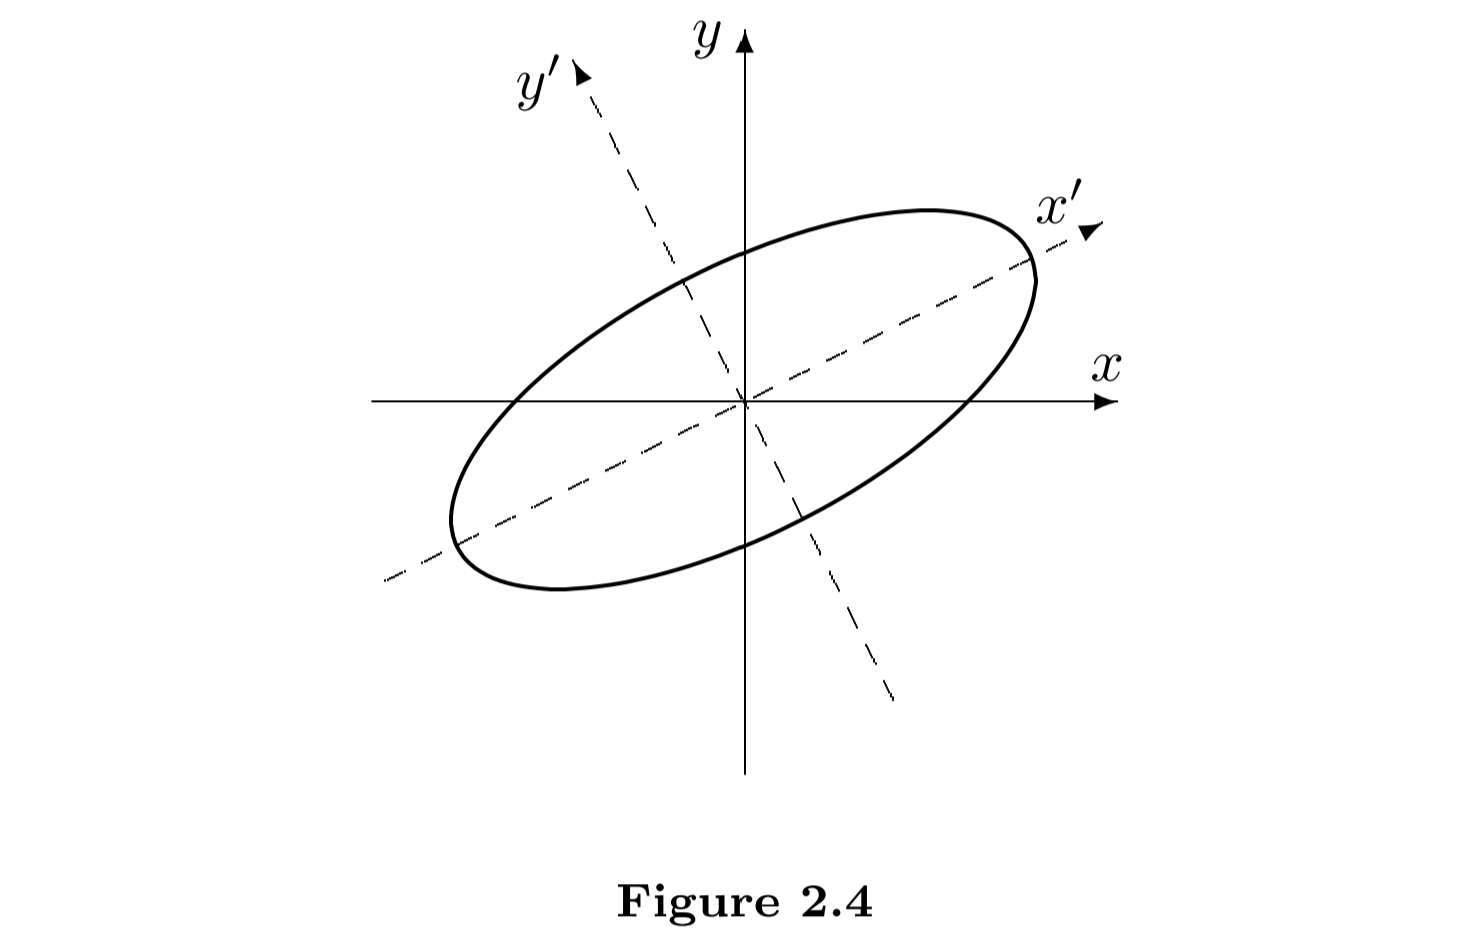
\includegraphics[width=10cm]{images/figure-2-4.png}

We will see how this change of variable is \emph{determined} in \SEC{6.5}.

(For figure 2.4,) Geometrically, the change of variable
\[
    P = \begin{pmatrix} x \\ y \end{pmatrix} \to \begin{pmatrix} x' \\ y' \end{pmatrix}
\]
is a \emph{change in the way} that the position of a point \(P\) in the plane is \emph{described}.
This is done by \emph{introducing a new frame of reference}, an \(x'y'\)-coordinate system with coordinate axes \emph{rotated} from the original \(xy\)-coordinate axes.
In this case, the new coordinate axes(\(x'\)-axis and \(y'\)-axis) are chosen to \emph{lie in the direction of the axes} of the ellipse.
The \textbf{unit vectors} along the \(x'\)-axis and the \(y'\)-axis form an \emph{ordered basis} for \(\SET{R}^2\):
\[
    \beta' = \bigg\{ \frac{1}{\sqrt{5}} \begin{pmatrix} 2 \\ 1 \end{pmatrix}, \frac{1}{\sqrt{5}} \begin{pmatrix} -1 \\ 2 \end{pmatrix} \bigg\}
\]
and the change of variable is actually a change from \([P]_{\beta} = \begin{pmatrix} x \\ y \end{pmatrix}\), the coordinate vector of \(P\) relative to the \emph{standard} ordered basis \(\beta = \{ e_1, e_2 \}\), to \([P]_{\beta'} = \begin{pmatrix} x' \\ y' \end{pmatrix}\), the coordinate vector of \(P\) relative to the new rotated basis \(\beta'\).

A natural question arises:
How can a coordinate vector relative to one basis be changed into a coordinate vector relative to the other?
Notice that the \emph{system of equations} relating the new and old coordinates can be represented by the matrix equation
\[
    \begin{pmatrix} x \\ y \end{pmatrix}
    = \frac{1}{\sqrt{5}} \begin{pmatrix}
        2 & -1 \\ 1 & 2
    \end{pmatrix} \begin{pmatrix} x' \\ y' \end{pmatrix}.
\]
Notice also that
\[
    Q = \frac{1}{\sqrt{5}} \begin{pmatrix}
        2 & -1 \\ 1 & 2
    \end{pmatrix}
\]
equals \([\mathrm{I}]_{\beta'}^{\beta}\), where \(\mathrm{I}\) denotes the \emph{identity transformation} on \(\SET{R}^2\).
Thus \([v]_{\beta} = Q[v]_{\beta'}\) for all \(v \in \SET{R}^2\).
(Also notice the \textbf{order} of the bases of the matrix representation;
the matrix representation is from the basis we want to change into the basis we originally have.)
A similar result is true in general.

\begin{theorem} \label{thm 2.22}
Let \(\beta\) and \(\beta'\) be two ordered bases for a finite-dimensional vector space \(V\), and let \(Q = [\ITRANV]_{\beta'}^{\beta}\).
Then
\begin{enumerate}
\item \(Q\) is invertible.
\item For any \(v \in V\), \([v]_{\beta} = Q[v]_{\beta'}\).
\end{enumerate}
\end{theorem}

\begin{proof} \ 

\begin{enumerate}
\item Since \(\ITRANV\) is invertible, \(Q\) is invertible by \THM{2.18}.

\item For any \(v \in V\),
\begin{align*}
    [v]_{\beta} & = [\ITRANV(v)]_{\beta} & \text{of course} \\
                & = [\ITRANV]_{\beta'}^{\beta} [v]_{\beta'} & \text{by \THM{2.14}} \\
                & = Q [v]_{\beta'}.
\end{align*}
\end{enumerate}
\end{proof}

\begin{remark} \label{remark 2.5.1}
The matrix \(Q = [\ITRANV]_{\beta'}^{\beta}\), defined in \THM{2.22}, is called \textbf{a change of coordinate matrix}.
Because of part (b) of the theorem, we say that \textbf{\(Q\) changes \(\beta'\)-coordinates into \(\beta\)-coordinates}.
Observe that if \(\beta = \{ x_1, x_2, ..., x_n \}\) and \(\beta' = \{ x'_1, x'_2, ..., x'_n \}\), then by definition of matrix representation, the \(j\)th column of \(Q = [\ITRANV]_{\beta'}^{\beta}\) is \([\ITRANV(x'_j)]_{\beta}\).
But since \([\ITRANV(x'_j)]_{\beta} = [x'_j]_{\beta}\), the \(j\)th column of \(Q\) is \([x'_j]_{\beta}\).
\end{remark}

\begin{note}
上面那段\ remark 是想表達,給定一個從原座標\ \(\beta'\) 轉換到目標座標\ \(\beta\) 的轉換矩陣,該矩陣的第\ \(j\) 行就是原座標\ \(\beta'\) 的第\ \(j\) 個\ vector,在用目標座標\ \(\beta\) 來表示時的座標向量。
\end{note}

Also notice that if \(Q\) changes \(\beta'\)-coordinates into \(\beta\)-coordinates, then \(Q^{-1}\) changes \(\beta\)-coordinates into \(\beta'\)-coordinates. (See \EXEC{2.5.11}.)

\begin{example} \label{example 2.5.1}
In \(\SET{R}^2\), let \(\beta = \{ (1, 1), (1, -1) \}\) and \(\beta' = \{ (2, 4), (3, 1) \}\).
Since
\[
    (2, 4) = 3(1, 1) - 1(1, - 1) \text{ and } (3, 1) = 2(1, 1) + 1(1, -1),
\]
The matrix that changes \(\beta\)'-coordinates into \(\beta\)-coordinates is
\[
    Q = \begin{pmatrix} 3 & 2 \\ -1 & 1 \end{pmatrix}.
\]
Thus, for instance, given a \emph{(normal) vector} \((2, 4) \in \SET{R}^2\),
\begin{align*}
    [(2, 4)]_{\beta} & = Q[(2, 4)]_{\beta'} & \text{by \THM{2.22}} \\
                     & = Q \begin{pmatrix} 1 \\ 0 \end{pmatrix} & \text{since \((2, 4)\) is the first vector of \(\beta'\)} \\
                     & = \begin{pmatrix} 3 \\ -1 \end{pmatrix} & \text{by calculation}
\end{align*}
\end{example}

\begin{note}
\((2, 4)\) in this example is \textbf{not} considered to be a coordinate vector; it simply is a ``normal'' vector of \(\SET{R}^2\).
However, \(\begin{pmatrix} 3 \\ -1 \end{pmatrix}\) is a coordinate vector;
if we consider a vector to be a coordinate vector, we write its components vertically, or horizontally but adding transpose to it.
\end{note}

For the remainder of this section, we consider only \LTRAN{}s that map a vector space \(V\) \emph{into itself}.
Such a \LTRAN{} is called a \textbf{linear operator} on \(V\).
(I have defined the term in \DEF{2.1}.)

Now suppose now that \(\T\) is a linear operator on a finite-dimensional vector space \(V\) and that \(\beta\) and \(\beta'\) are ordered bases for \(V\).
Then \(V\) can be represented by the matrices \([\T]_{\beta}\) and \([\T]_{\beta'}\).
What is the \emph{relationship} between these matrices?
The next theorem provides a simple answer using a
change of coordinate matrix.

\begin{theorem} \label{thm 2.23}
Let \(\T\) be a linear operator on a finite-dimensional vector space \(V\),
and let \(\beta\) and \(\beta'\) be ordered bases for \(V\).
Suppose that \(Q\) is the change of coordinate matrix that changes \(\beta'\)-coordinates into \(\beta\)-coordinates.
Then
\[
    [\T]_{\beta} = Q^{-1} [\T]_{\beta'} Q.
\]
\end{theorem}

\begin{note}
Related exercise: \EXEC{2.4.16}.
\end{note}

\begin{proof}
Let \(\ITRANV\) be the identity transformation on \(V\).
Then
\begin{align*}
    Q [\T]_{\beta'} & = [\ITRANV]_{\beta'}^{\beta} [\T]_{\beta'} & \text{by def of \(Q\)} \\
                    & = [\ITRANV \T]_{\beta'}^{\beta} & \text{by \THM{2.11}} \\
                    & = [\T \ITRANV]_{\beta'}^{\beta} & \text{by \THM{2.10}(c)} \\
                    & = [\T]_{\beta} [\ITRANV]_{\beta'}^{\beta} & \text{by \THM{2.11}} \\
                    & = [\T]_{\beta} Q & \text{by def of \(Q\)}
\end{align*}
which implies
\begin{align*}
             & Q [\T]_{\beta'} = [\T]_{\beta} Q \\
    \implies & Q^{-1} Q [\T]_{\beta'} = Q^{-1} [\T]_{\beta} Q & \text{by multiplying \(Q^{-1}\) on the left} \\
    \implies & [\T]_{\beta'} = Q^{-1} [\T]_{\beta} Q. & \text{of course}
\end{align*}
\end{proof}

\begin{example} \label{example 2.5.2}
Let \(\T\) be the linear operator on \(\SET{R}^2\) defined by
\[
    \T \begin{pmatrix} a \\ b \end{pmatrix} = \begin{pmatrix} 3a - b \\ a + 3b \end{pmatrix}
\]
let \(\beta = \{ (1, 1), (1, -1) \}\) and \(\beta' = \{ (2, 4), (3, 1) \}\).
The reader should verify that
\[
    [\T]_{\beta} = \begin{pmatrix} 3 & 1 \\ -1 & 3 \end{pmatrix}
\]
In \EXAMPLE{2.5.1}, we saw that the change of coordinate matrix that changes \(\beta'\)-coordinates into \(\beta\)-coordinates is
\[
    Q = \begin{pmatrix} 3 & 2 \\ -1 & 1 \end{pmatrix}.
\]
and it is easily verified that
\[
    Q^{-1} = \frac{1}{5} \begin{pmatrix} 1 & -2 \\ 1 & 3 \end{pmatrix}.
\]
Hence, by \THM{2.23},
\[
    [\T]_{\beta'} = Q^{-1} [\T]_{\beta} Q = \begin{pmatrix} 4 & 1 \\ -2 & -2 \end{pmatrix}.
\]
To show that this \([\T]_{\beta'}\) is really the correct matrix, we can verify that the image under \(\T\) of each vector of \(\beta'\) is the linear combination of the vectors of \(\beta'\) with the entries of the corresponding column as this \([\T]_{\beta'}\)'s coefficients.
For example, the image of the \emph{second} vector in \(\beta'\) is
\[
    \T \begin{pmatrix} 3 & 1 \end{pmatrix} = \begin{pmatrix} 8 & 6 \end{pmatrix} = \RED{1} \begin{pmatrix} 2 & 4 \end{pmatrix} + \RED{3} \begin{pmatrix} 3 & 1 \end{pmatrix}
\]
Notice that the coefficients of the linear combination are the entries of the \emph{second} column of this \([\T]_{\beta'}\).
\end{example}

\begin{note}
It is often useful to apply \THM{2.23} to compute \([\T]_{\beta}\), as the next example shows.
\end{note}

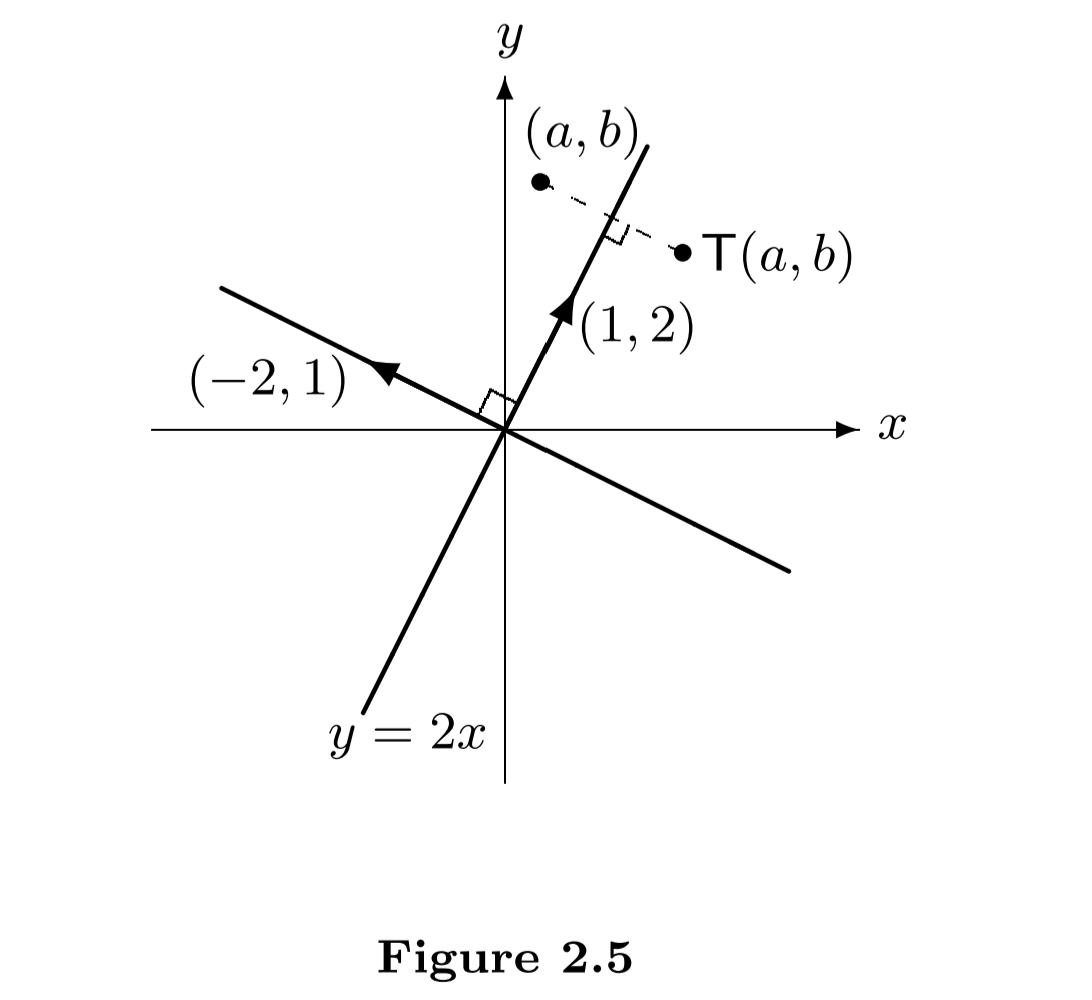
\includegraphics[width=8cm]{images/figure-2-5.png}

\begin{example} \label{example 2.5.3}
Recall the \emph{reflection} about the \(x\)-axis in \EXAMPLE{2.1.3}.
The rule \((x, y) \to (x, -y)\) is easy to obtain.
We now derive the less obvious rule for the \emph{reflection} \(\T\) \emph{about the line} \(y = 2x\). (See Figure 2.5.)

We wish to find \emph{an expression} for \(\T(a,b)\) for any \((a,b) \in \SET{R}^2\).
Since \(\T\) is linear, (by \THM{2.6}) it is completely
determined by its values on \emph{a basis} for \(\SET{R}^2\).
Clearly, from figure 2.5 we have \(\T(1, 2) = (1, 2) = 1 \cdot (1, 2) + 0 \cdot (-2, 1)\) and \(\T(-2, 1) = -(-2, 1) = 0 \cdot (1, 2) + (-1) \cdot (-2, 1)\), where \(\{ (1, 2), (-2, 1) \}\) is a basis for \(\SET{R}^2\).
Then we let \(\beta' = \{ (1, 2), (-2, 1) \}\), from these result (and \THM{2.6}),
\[
    [\T]_{\beta'} = \begin{pmatrix} 1 & 0 \\ 0 & -1 \end{pmatrix}.
\]

Now let \(\beta\) be the \emph{standard} ordered basis for \(\SET{R}^2\), and let \(Q\) be the matrix that changes \(\beta'\)-coordinates into \(\beta\)-coordinates.

Then (by calculation),
\[
    Q = \begin{pmatrix} 1 & -2 \\ 2 & 1 \end{pmatrix}
\]
And from \THM{2.23} and some calculation(see \EXEC{2.5.1}(c)) we have \([\T]_{\beta} = Q[\T]_{\beta'}Q^{-1}\).
Because (mysteriously)
\[
    Q^{-1} = \frac{1}{5} \begin{pmatrix} 1 & 2 \\ -2 & 1 \end{pmatrix}
\]
the reader can verify that
\[
    [\T]_{\beta} = \frac{1}{5} \begin{pmatrix} -3 & 4 \\ 4 & 3 \end{pmatrix}
\]
Since \(\beta\) is the standard ordered basis, it follows by \THM{2.15}(a) that \(\T\) is left-multiplication by \([\T]_{\beta}\).
Thus for any \((a, b) \in \SET{R}^2\), we have
\[
    \T \begin{pmatrix} a \\ b \end{pmatrix}
    = \frac{1}{5} \begin{pmatrix} -3 & 4 \\ 4 & 3 \end{pmatrix} \begin{pmatrix} a \\ b \end{pmatrix}
    = \frac{1}{5} \begin{pmatrix} -3a + 4b \\ 4a + 3b \end{pmatrix}.
\]
\end{example}

A useful special case of \THM{2.23} is contained in the next corollary.

\begin{corollary} \label{corollary 2.23.1}
Let \(A \in M_{n \X n}(F)\), and let \(\gamma\) be an ordered basis for \(F^n\).
Then \([\LMTRAN_A]_{\gamma} = Q^{-1} A Q\), where \(Q\) is the \(n \X n\) matrix whose \(j\)th column is the \(j\)th vector of \(\gamma\).
\end{corollary}

\begin{proof}
Let \(\beta\) be the \emph{standard} ordered basis for \(F^n\), then by \THM{2.15}(a), \([\LMTRAN_A]_{\beta} = A\).
Then by \THM{2.23}, \([\LMTRAN_A]_{\gamma} = Q^{-1} [\LMTRAN_A]_{\beta} Q\) where \(Q\) is the coordinate matrix that changes \(\gamma\)-coordinates into \(\beta\)-coordinates.
And from \RMK{2.5.1}, the \(j\)th column of \(Q\) is \([v_j]_{\beta}\) where \(v_j\) is the \(j\)th vector of \(\gamma\).
But since \(\beta\) is standard ordred basis, we have \([v_j]_{\beta} = v_j\), so the \(j\)th column of \(Q\) is \(v_j\), as desired.
\end{proof}

\begin{note}
這個\ corollary 是\ \RMK{2.5.1} 的「更加\ special case」:
當我們把某個基底座標\textbf{轉換成標準基底座標},則那個座標轉換矩陣的第\ \(j\) 行就直接等於那個基底座標的第\ \(j\) 個向量。
\end{note}

\begin{example} \label{example 2.5.4}
Let
\[
    A = \begin{pmatrix}
        2 & 1 & 0 \\ 1 & 1 & 3 \\ 0 & -1 & 0
    \end{pmatrix},
\]
and let
\[
    \gamma = \bigg\{
        \begin{pmatrix} -1 \\ 0 \\ 0 \end{pmatrix}, 
        \begin{pmatrix} 2 \\ 1 \\ 0 \end{pmatrix}, 
        \begin{pmatrix} 1 \\ 1 \\ 1 \end{pmatrix}
    \bigg\},
\]
which is an ordered basis for \(\SET{R}^3\).
Let \(Q\) be the \(3 \X 3\) matrix whose \(j\)th column is the \(j\)th vector of \(\gamma\). (this satisfies the condition of \CORO{2.23.1}.)
Then
\[
    Q = \begin{pmatrix} -1 & 2 & 1 \\ 0 & 1 & 1 \\ 0 & 0 & 1 \end{pmatrix}
    \text{ and (mysteriously) }
    Q^{-1} = \begin{pmatrix} -1 & 2 & -1 \\ 0 & 1 & -1 \\ 0 & 0 & 1 \end{pmatrix}.
\]
So by \CORO{2.23.1},
\[
    [\LMTRAN_A]_{\gamma} = Q^{-1} A Q = \begin{pmatrix} 0 & 2 & 8 \\ -1 & 4 & 6 \\ 0 & -1 & -1 \end{pmatrix}.
\]
\end{example}

\begin{remark} \label{remark 2.5.2}
The relationship, defined immediately, between the matrices \([\T]_{\beta'}\) and \([\T]_{\beta}\) in \THM{2.23} \textbf{will be the subject of further study in Chapters 5, 6, and 7}.
\end{remark}

\begin{definition} \label{def 2.16}
Let \(A\) and \(B\) be matrices in \(M_{n \X n}(F)\).
We say that \(B\) is \textbf{similar}\textbf{} to \(A\) if there exists an \textbf{invertible matrix} \(Q\) such that \(B = Q^{-1} A Q\).
\end{definition}

\begin{remark} \label{remark 2.5.3}
Observe that the relation of similarity is an \textbf{equivalence relation} (see \EXEC{2.5.9}).
So we need only say that \(A\) and \(B\) are similar.

Notice also that in this terminology \THM{2.23} can be stated as follows:
If \(\T\) is a linear operator on a finite-dimensional vector space \(V\), and if \(\beta\) and \(\beta'\) are any ordered bases for \(V\), then \([\T]_{\beta'}\) is similar to \([\T]_{\beta}\).
\end{remark}

\begin{remark} \label{remark 2.5.4}
\THM{2.23} can be \emph{generalized} to allow \(\T : V \to W\), where \(V\) is distinct from \(W\).
In this case, we can change bases in \(V\) as well as in \(W\) (see \EXEC{2.5.8}).
\end{remark}

\exercisesection

\begin{exercise} \label{exercise 2.5.1}
Label the following statements as true or false.
\begin{enumerate}
\item Suppose that \(\beta = \{ x_1, x_2, ..., x_n \}\) and \(\beta' = \{ x'_1, x'_2, ..., x'_n \}\) are ordered bases for a vector space
and \(Q\) is the change of coordinate matrix that changes \(\beta'\)-coordinates into \(\beta\)-coordinates.
Then the \(j\)th column of \(Q\) is \([x_j]_{\beta'}\).

\item Every change of coordinate matrix is invertible. 

\item Let \(\T\) be a linear operator on a finite-dimensional vector space \(V\), let \(\beta\) and \(\beta'\) be ordered bases for \(V\),
and let \(Q\) be the change of coordinate matrix that changes \(\beta'\)-coordinates into \(\beta\)-coordinates.
Then \([\T]_{\beta} = Q [\T]_{\beta'} Q^{-1}\).

\item The matrices \(A, B \in M_{n \X n}(F)\) are called similar if \(B = Q^\top A Q\) for some \(Q \in M_{n \X n}(F)\).

\item Let \(\T\) be a linear operator on a finite-dimensional vector space \(V\).
Then for any ordered bases \(\beta\) and \(\gamma\) for \(V\), \([\T]_{\beta}\) is similar to \([\T]_{\gamma}\).
\end{enumerate}
\end{exercise}

\begin{proof} \ 

\begin{enumerate}
\item False. By \RMK{2.5.1}, the \(j\)th column of \(Q\) is \([x'_j]_{\beta}\).
\item True by \THM{2.22}(a).
\item True.
    We have
    \begin{align*}
                 & [\T]_{\beta'} = Q^{-1}[\T]_{\beta}Q & \text{by \THM{2.23}} \\
        \implies & Q [\T]_{\beta'} Q^{-1} = Q (Q^{-1} [\T]_{\beta} Q) Q^{-1} & \text{by multiplying \(Q\) in the left and \(Q^{-1}\) in the right} \\
        \implies & Q [\T]_{\beta'} Q^{-1} = [\T]_{\beta},
    \end{align*}
    as desired.
\item False by \DEF{2.16}.
\item True by \RMK{2.5.3}.
\end{enumerate}
\end{proof}

\begin{exercise} \label{exercise 2.5.2}
For each of the following pairs of ordered bases \(\beta\) and \(\beta'\) for \(\SET{R}^2\), find the change of coordinate matrix that changes \(\beta'\)-coordinates into \(\beta\)-coordinates.
\begin{enumerate}
\item \(\beta = \{ e_1, e_2 \}\) and \(\beta' = \{ (a_1, a_2), (b_1, b_2) \}\).
\item \(\beta = \{ (-1, 3), (2, -1) \}\) and \(\beta' = \{ (0, 10), (5, 0) \}\).
\item \(\beta = \{ (2, 5), (-1, -3) \}\) and \(\beta' = \{ e_1, e_2 \}\).
\item \(\beta = \{ (-4, 3), (2, -1) \}\) and \(\beta' = \{ (2, 1), (-4, 1) \}\).
\end{enumerate}
\end{exercise}

\begin{proof} \ 

\begin{enumerate}
\item We have \((a_1, a_2) = a_1 \cdot e_1 + a_2 \cdot e_2\), \((b_1, b_2) = b_1 \cdot e_1 + b_2 \cdot e_2\), so
\[ Q = \begin{pmatrix} a_1 & b_1 \\ a_2 & b_2 \end{pmatrix}. \]

\item (By solving system of equations), \((0, 10) = 4 \cdot (-1, 3) + 2 \cdot (2, -1)\), \((5, 0) = 1 \cdot (-1, 3) + 3 \cdot (2, -1)\), so
\[ Q = \begin{pmatrix} 4 & 1 \\ 2 & 3 \end{pmatrix}. \]

\item (By solving system of equations), \(e_1 = 3 \cdot (2, 5) + 5 \cdot (-1, -3)\), \(e_2 = -1 \cdot (2, 5) + (-2) \cdot (-1, -3)\), so
\[ Q = \begin{pmatrix} 3 & -1 \\ 5 & -2 \end{pmatrix}. \]

\item (By solving system of equations), \((2, 1) = 2 \cdot (-4, 3) + 5 \cdot (2, -1)\), \((-4, 1) = -1 \cdot (-4, 3) + (-4) \cdot (2, -1)\), so
\[ Q = \begin{pmatrix} 2 & -1 \\ 5 & -4 \end{pmatrix}. \]
\end{enumerate}
\end{proof}

\begin{exercise} \label{exercise 2.5.3}
Skip, tedious.
\end{exercise}

\begin{exercise} \label{exercise 2.5.4}
Let \(\T\) be the linear operator on \(\SET{R}^2\) defined by
\[
    \T\begin{pmatrix} a \\ b \end{pmatrix}
    = \begin{pmatrix} 2a + b \\ a - 3b \end{pmatrix},
\]
let \(\beta\) be the standard ordered basis for \(\SET{R}^2\), and let
\[
    \beta' = \bigg\{ \begin{pmatrix} 1 \\ 1 \end{pmatrix},
    \begin{pmatrix} 1 \\ 2 \end{pmatrix} \bigg\}.
\]
Use \THM{2.23} and the (mysterious) fact that
\[
    \begin{pmatrix} 1 & 1 \\ 1 & 2 \end{pmatrix}^{-1} =
    \begin{pmatrix} 2 & -1 \\ -1 & 1 \end{pmatrix}
\]
to find \([\T]_{\beta'}\).
\end{exercise}

\begin{proof}
First \([\T]_{\beta} = \begin{pmatrix} 2 & 1 \\ 1 & -3 \end{pmatrix}\), since \(\T(e_1) = \begin{pmatrix} 2 \\ 1 \end{pmatrix}= 2 \cdot e_1 + 1 \cdot e_2\) and \(\T(e_2) = \begin{pmatrix} 1 \\ -3 \end{pmatrix} = 1 \cdot e_1 + (-3) \cdot e_2\).
And by solving equation we know \(Q = \begin{pmatrix} 1 & 1 \\ 1 & 2 \end{pmatrix}\).
Then by \THM{2.23} and the provided fact,
\[
    [\T]_{\beta'} = Q^{-1} [\T]_{\beta} Q =
    \begin{pmatrix} 2 & -1 \\ -1 & 1 \end{pmatrix}
    \begin{pmatrix} 2 & 1 \\ 1 & -3 \end{pmatrix}
    \begin{pmatrix} 1 & 1 \\ 1 & 2 \end{pmatrix}
    = \begin{pmatrix} 8 & 13 \\ -5 & -9 \end{pmatrix}
\]
\end{proof}

\begin{exercise} \label{exercise 2.5.5}
Let \(\T\) be the linear operator on \(\mathcal{P}_1(\SET{R})\) defined by \(\T(p(x)) = p'(x)\), the derivative of \(p(x)\).\
Let \(\beta = \{ 1, x \}\) and \(\beta' = \{ 1 + x, 1 - x \}\).
Use \THM{2.23} and the fact that
\[
    \begin{pmatrix} 1 & 1 \\ 1 & -1 \end{pmatrix}^{-1} =
    \begin{pmatrix} \frac1{2} & \frac1{2} \\ \frac1{2} & -\frac1{2} \end{pmatrix}
\]
to find \([\T]_{\beta'}\).
\end{exercise}

\begin{proof}

First \([\T]_{\beta} = \begin{pmatrix} 0 & 1 \\ 0 & 0 \end{pmatrix}\) since \(\T(1) = 0 = 0 \cdot 1 + 0 \cdot x\) and \(\T(x) = 1 = 1 \cdot 1 + 0 \cdot x\).
And by solving equation we know \(Q = \begin{pmatrix} 1 & 1 \\ 1 & -1 \end{pmatrix}\).
Then by \THM{2.23} and the provided fact,
\[
    [\T]_{\beta'} = Q^{-1} [\T]_{\beta} Q =
    \begin{pmatrix} \frac1{2} & \frac1{2} \\ \frac1{2} & -\frac1{2} \end{pmatrix}
    \begin{pmatrix} 0 & 1 \\ 0 & 0 \end{pmatrix}
    \begin{pmatrix} 1 & 1 \\ 1 & -1 \end{pmatrix}
    = \begin{pmatrix} \frac1{2} & -\frac1{2} \\ \frac1{2} & -\frac1{2} \end{pmatrix}
\]
\end{proof}

\begin{exercise} \label{exercise 2.5.6}
For each matrix \(A\) and ordered basis \(\beta\), find \([\LMTRAN_A]_{\beta}\).
Also, find an invertible matrix \(Q\) such that \([\LMTRAN_A]_{\beta} = Q^{-1} A Q\).

\begin{enumerate}
\item \(A = \begin{pmatrix} 1 & 3 \\ 1 & 1 \end{pmatrix}\) and \(\beta = \bigg\{
    \begin{pmatrix} 1 \\ 1 \end{pmatrix},
    \begin{pmatrix} 1 \\ 2 \end{pmatrix}
\bigg\}\)

\item \(A = \begin{pmatrix} 1 & 2 \\ 2 & 1 \end{pmatrix}\) and \(\beta = \bigg\{
    \begin{pmatrix} 1 \\ 1 \end{pmatrix},
    \begin{pmatrix} 1 \\ -1 \end{pmatrix}
\bigg\}\)

\item \(A = \begin{pmatrix} 1 & 1 & -1 \\ 2 & 0 & 1 \\ 1 & 1 & 0 \end{pmatrix}\) and \(\beta = \bigg\{
    \begin{pmatrix} 1 \\ 1 \\ 1 \end{pmatrix},
    \begin{pmatrix} 1 \\ 0 \\ 1 \end{pmatrix},
    \begin{pmatrix} 1 \\ 1 \\ 2 \end{pmatrix}
\bigg\}\)

\item \(A = \begin{pmatrix} 13 & 1 & 4 \\ 1 & 13 & 4 \\ 4 & 4 & 10 \end{pmatrix}\) and \(\beta = \bigg\{
    \begin{pmatrix} 1 \\ 1 \\ -2 \end{pmatrix},
    \begin{pmatrix} 1 \\ -1 \\ 0 \end{pmatrix},
    \begin{pmatrix} 1 \\ 1 \\ 1 \end{pmatrix}
\bigg\}\)
\end{enumerate}
\end{exercise}

\begin{proof}
From \CORO{2.23.1}, \([\LMTRAN_A]_{\beta} = Q^{-1} A Q\), where \(Q\) is the \(n \X n\) matrix whose \(j\)th column is the \(j\)th vector of \(\beta\).
Hence

\begin{enumerate}
\item \(Q = \begin{pmatrix} 1 & 1 \\ 1 & 2 \end{pmatrix}\).

\item \(Q = \begin{pmatrix} 1 & 1 \\ 1 & -1 \end{pmatrix}\).

\item \(Q = \begin{pmatrix} 1 & 1 & 1 \\ 1 & 0 & 1 \\ 1 & 1 & 2 \end{pmatrix}\).

\item \(Q = \begin{pmatrix} 1 & 1 & 1 \\ 1 & -1 & 1 \\ -2 & 0 & 1 \end{pmatrix}\).
\end{enumerate}

I skip computing \([\LMTRAN_A]_{\beta}\), since either computing it directly or using \CORO{2.23.1} but requiring \(Q^{-1}\) are tedious.
\end{proof}

\begin{exercise} \label{exercise 2.5.7}
In \(\SET{R}^2\), let \(L\) be the line \(y = mx\), where \(m \ne 0\).
Find an expression for \(\T(x, y)\), where
\begin{enumerate}
\item \(\T\) is the reflection of \(\SET{R}^2\) about \(L\).
\item \(\T\) is the projection(see \ADEF{2.2}) on \(L\) along the line \emph{perpendicular} to \(L\).
\end{enumerate}
\end{exercise}

\begin{proof}
We may let \(\beta\) be the standard ordered basis and \(\alpha = \{ (1, m), (-m, 1) \}\) be another basis for \(\SET{R}^2\).
\begin{enumerate}
\item We have that \([\T]_{\alpha} = \begin{pmatrix} 1 & 0 \\ 0 & -1 \end{pmatrix}\) and (by \EXEC{2.5.11}) \(Q^{-1} = [\mathrm{I}]_{\alpha}^{\beta} = \begin{pmatrix} 1 & m \\ -m & 1 \end{pmatrix}\).
We can also calculate that \(Q = [\mathrm{I}]_{\beta}^{\alpha} = \begin{pmatrix} \frac{1}{m^2 + 1} & \frac{m}{m^2 + 1} \\ -\frac{m}{m^2 + 1} & \frac{1}{m^2 + 1} \end{pmatrix}\).
So by \THM{2.23}, we have
\[
    [\T]_{\beta} = Q^{-1} [\T]_{\alpha} Q = \begin{pmatrix}
        \frac{1 - m^2}{m^2 + 1} & \frac{2m}{m^2 + 1} \\
        \frac{2m}{m^2 + 1} & \frac{m^2 - 1}{m^2 + 1}
    \end{pmatrix}.
\]
And we have
\begin{align*}
    & \T \begin{pmatrix} x \\ y \end{pmatrix} \\
    & = \left[ \T \begin{pmatrix} x \\ y \end{pmatrix} \right]_{\beta} & \text{since domain/codomain are actually \(\SET{R}^n\) and \(\beta\) is standard} \\
    & = [\T]_{\beta} \left[ \begin{pmatrix} x \\ y \end{pmatrix} \right]_{\beta} & \text{by \THM{2.14}} \\
    & = [\T]_{\beta} \begin{pmatrix} x \\ y \end{pmatrix} & \text{since domain/codomain are actually \(\SET{R}^n\) and \(\beta\) is standard} \\
    & = \begin{pmatrix}
            \frac{1 - m^2}{m^2 + 1} & \frac{2m}{m^2 + 1} \\
            \frac{2m}{m^2 + 1} & \frac{m^2 - 1}{m^2 + 1}
        \end{pmatrix}
        \begin{pmatrix} x \\ y \end{pmatrix} \\
    & = \begin{pmatrix}
            \frac{x-m^{2} x+2 m y}{1+m^{2}} \\
            \frac{2 m x+m^{2} y-y}{1+m^{2}}
        \end{pmatrix}
\end{align*}

\item Similarly we have that \([\T]_{\alpha} = \begin{pmatrix} 1 & 0 \\ 0 & 0 \end{pmatrix}\).
And with the same \(Q^{-1}\) and \(Q\) we have
\[
    [\T]_{\beta} = Q^{-1} [\T]_{\alpha} Q = \begin{pmatrix}
        \frac{1}{m^2 + 1} & \frac{m}{m^2 + 1} \\
        \frac{m}{m^2 + 1} & \frac{m^2}{m^2 + 1}
    \end{pmatrix}.
\]
So 
\begin{align*}
    & \T \begin{pmatrix} x \\ y \end{pmatrix} \\
    & = [\T]_{\beta} \begin{pmatrix} x \\ y \end{pmatrix} & \text{similar derivation from part(a)} \\
    & = \begin{pmatrix}
            \frac{1}{m^2 + 1} & \frac{m}{m^2 + 1} \\
            \frac{m}{m^2 + 1} & \frac{m^2}{m^2 + 1}
        \end{pmatrix}
        \begin{pmatrix} x \\ y \end{pmatrix} \\
    & = \begin{pmatrix}
            \frac{x + ym}{m^{2} + 1} \\
            \frac{xm + ym^2}{m^{2} + 1}
        \end{pmatrix}
\end{align*}

\end{enumerate}
\end{proof}

\begin{exercise} \label{exercise 2.5.8}
Prove the following \emph{generalization} of \THM{2.23}.
Let \(\T : V \to W\) be a \LTRAN{} from a finite-dimensional vector space \(V\) to a finite-dimensional vector space \(W\).
Let \(\beta\) and \(\beta'\) be ordered bases for \(V\), and let \(\gamma\) and \(\gamma'\) be ordered bases for \(W\).
Then \([\T]_{\beta'}^{\gamma'} = P^{-1} [\T]_{\beta}^{\gamma} Q\), where \(Q\) is the matrix that changes \(\beta'\)-coordinates into \(\beta\)-coordinates and \(P\) is the matrix that changes \(\gamma'\)-coordinates into \(\gamma\)-coordinates.
\end{exercise}

\begin{proof}
By (the generalization of) \THM{2.10}(c), we have \(\T = \ITRANW \T = \T \ITRANV\) \MAROON{(1)}.

Then we have
\begin{align*}
    P [\T]_{\beta'}^{\gamma'}
        & = [\ITRANW]_{\gamma'}^{\gamma} [\T]_{\beta'}^{\gamma'} & \text{by def of \(P\)} \\
        & = [\ITRANW\T]_{\beta'}^{\gamma} & \text{by \THM{2.11}} \\
        & = [\T\ITRANV]_{\beta'}^{\gamma} & \text{by \MAROON{(1)}} \\
        & = [\T]_{\beta}^{\gamma} [\ITRANV]_{\beta'}^{\beta} & \text{\THM{2.11}} \\
        & = [\T]_{\beta}^{\gamma} Q & \text{by def of \(Q\)}
\end{align*}
So we have \(P [\T]_{\beta'}^{\gamma'} = [\T]_{\beta}^{\gamma} Q\).
And
\begin{align*}
             & P [\T]_{\beta'}^{\gamma'} = [\T]_{\beta}^{\gamma} Q \\
    \implies & P^{-1} P [\T]_{\beta'}^{\gamma'} = P^{-1} [\T]_{\beta}^{\gamma} Q & \text{by multiplying \(P^{-1}\) in the left} \\
    \implies & [\T]_{\beta'}^{\gamma'} = P^{-1} [\T]_{\beta}^{\gamma} Q, & \text{of course}
\end{align*}
as desired.
\end{proof}

\begin{exercise} \label{exercise 2.5.9}
Prove that "is similar to" is an equivalence relation on \(M_{n \X n}(F)\).
\end{exercise}

\begin{proof}
For any \(n \X n\) matrix \(A\), it is similar to itself since \(A = IAI\).

Suppose \(A\) is similar to \(B\), then by \DEF{2.16} we have an invertible matrix \(Q\) s.t. \(A = Q^{-1}BQ\).
Then
\begin{align*}
             & A = Q^{-1}BQ \\
    \implies & Q A Q^{-1} = Q (Q^{-1} B Q) Q^{-1} \\
    \implies & Q A Q^{-1} = B \\
    \implies & (Q^{-1})^{-1} A Q^{-1} = B.
\end{align*}
So we have an invertible matrix \(Q^{-1}\) s.t. \(B = (Q^{-1})^{-1} A Q^{-1}\).
Then by \DEF{2.16}, \(B\) is similar to \(A\).

Suppose \(A\) is similar to \(B\), \(B\) is similar to \(C\).
Then by \DEF{2.16} we have an invertible matrix \(P\) s.t. \(A = P^{-1}BP\) and invertible matrix \(Q\) s.t. \(B = Q^{-1}CQ\)
Then by \ATHM{2.36}(2), \(QP\) is invertible and \((QP)^{-1} = P^{-1} Q^{-1}\) \MAROON{(1)}.
And
\begin{align*}
             & A = P^{-1}BP \\
    \implies & A = P^{-1} (Q^{-1} C Q) P \\
    \implies & A = (P^{-1} Q^{-1}) C (Q P) \\
    \implies & A = (Q P)^{-1} C (Q P) & \text{by \MAROON{(1)}}
\end{align*}
So we have an invertible matrix \(QP\) s.t. \(A = (QP)^{-1} C (QP)\).
So by \DEF{2.16}, \(A\) is similar to \(C\).
\end{proof}

\begin{exercise} \label{exercise 2.5.10} \ 

\begin{enumerate}
\item Prove that if \(A\) and \(B\) are similar \(n \X n\) matrices, then \(\TRACE(A) = \TRACE(B)\).
Hint: Use \ATHM{2.27}.
USEDINSEC5.2\#11.

\item How would you define the \emph{trace} of a linear operator on a finite-dimensional vector space?
Justify that your definition is well-defined.
\end{enumerate}
\end{exercise}

\begin{proof} \ 

\begin{enumerate}
\item
\begin{align*}
    \TRACE(A) & = \TRACE(\BLUE{Q^{-1}B}\RED{Q}) & \text{since \(A, B\) are similar} \\
              & = \TRACE(\RED{Q}\BLUE{Q^{-1}B}) & \text{by \ATHM{2.27}} \\
              & = \TRACE(B) & \text{of course}
\end{align*}

\item Given finite-dimensional vector space \(V\) and linear operator \(\T : V \to V\), we define \(\TRACE(\T) = \TRACE([\T]_{\beta})\) where \(\beta\) is a basis for \(V\).
The definition is well-defined because given arbitrary bases \(\beta, \beta'\) for \(V\), by \THM{2.23}, \([\T]_{\beta}\) and \([\T]_{\beta'}\) are similar, and by part(a), \(\TRACE([\T]_{\beta}) = \TRACE([\T]_{\beta'})\).
\end{enumerate}
\end{proof}

\begin{exercise} \label{exercise 2.5.11}
Let \(V\) be a finite-dimensional vector space with ordered bases \(\alpha, \beta\), and \(\gamma\).
\begin{enumerate}
\item Prove that if \(Q\) and \(R\) are the change of coordinate matrices that change \(\alpha\)-coordinates into \(\beta\)-coordinates and \(\beta\)-coordinates into \(\gamma\)-coordinates, respectively, then \(RQ\) is the change of coordinate matrix that changes \(\alpha\)-coordinates into \(\gamma\)-coordinates.

\item Prove that if \(Q\) changes \(\alpha\)-coordinates into \(\beta\)-coordinates, then \(Q^{-1}\) changes \(\beta\)-coordinates into \(\alpha\)-coordinates.
\end{enumerate}
\end{exercise}

\begin{proof} \ 
\begin{enumerate}
\item We have \(Q = [\mathrm{I}]_{\alpha}^{\beta}\) and \(R = [\mathrm{I}]_{\beta}^{\gamma}\).
So
\begin{align*}
    RQ = & [\mathrm{I}]_{\beta}^{\gamma} [\mathrm{I}]_{\alpha}^{\beta} \\
         & = [\mathrm{I}\mathrm{I}]_{\alpha}^{\gamma} & \text{by \THM{2.11}} \\
         & = [\mathrm{I}]_{\alpha}^{\gamma}, & \text{of course}
\end{align*}
which is the coordinate matrix that change \(\alpha\)-coordinates into \(\gamma\)-coordinates.

\item Again we have \(Q = [\mathrm{I}]_{\alpha}^{\beta}\).
Let \(I_n\) be \(n \X n\) identity matrix, then we have
\begin{align*}
    Q[\mathrm{I}]_{\beta}^{\alpha}
        & = [\mathrm{I}]_{\alpha}^{\beta}[\mathrm{I}]_{\beta}^{\alpha} \\
        & = [\mathrm{I}\mathrm{I}]_{\beta}^{\beta} & \text{by \THM{2.11}} \\
        & = [\mathrm{I}]_{\beta}^{\beta} & \text{of course} \\
        & = I_n, & \text{of course}
\end{align*}
and
\begin{align*}
    [\mathrm{I}]_{\beta}^{\alpha} Q
        & = [\mathrm{I}]_{\beta}^{\alpha} [\mathrm{I}]_{\alpha}^{\beta} \\
        & = [\mathrm{I}\mathrm{I}]_{\alpha}^{\alpha} & \text{by \THM{2.11}} \\
        & = [\mathrm{I}]_{\alpha}^{\alpha} & \text{of course} \\
        & = I_n, & \text{of course}
\end{align*}
hence by definition of \DEF{2.13}, \(Q^{-1}\) is \([\mathrm{I}]_{\beta}^{\alpha}\), that is, \(Q^{-1}\) is the coordinate matrix that changes \(\beta\)-coordinates into \(\alpha\)-coordinates.
\end{enumerate}
\end{proof}

\begin{exercise} \label{exercise 2.5.12}
Prove \CORO{2.23.1}.
\end{exercise}

\begin{proof}
See \CORO{2.23.1}.
\end{proof}

\begin{exercise} \label{exercise 2.5.13}
\sloppy Let \(V\) be a finite-dimensional vector space over a field \(F\), and let \(\beta = \{ x_1, x_2, ..., x_n \}\) be an ordered basis for \(V\).
Let \(Q\) be an \(n \X n\) \emph{invertible} matrix with entries from \(F\).
Define
\[
    x_j' = \sum_{i = 1}^n Q_{ij} x_i \text{ for } 1 \le j \le n,
\]
and set \(\beta' = \{ x_1', x_2', ..., x_n' \}\).
Prove that \(\beta'\) is a basis for \(V\) and hence that \(Q\) is the change of coordinate matrix that changes \(\beta'\)-coordinates into \(\beta\)-coordinates.
\end{exercise}

\begin{note}
The exercise with highly related concept: \EXEC{2.4.15}.
\end{note}

\begin{note}
這題背後的意義就是,若\ \(\beta\) 是\ basis,\(\T\) 是可逆變換(所以對應的矩陣也是可逆),則\ \(\T(\beta)\) 也是一個\ basis。
相關練習有\ \EXEC{2.4.15},不過這題是那個練習的\ special case,也就是\ codomain \(W = V\) 的情況。
\end{note}

\begin{proof}
First we show that \(\beta'\) is \LID{}.
So suppose \(a_1 x'_1 + a_2 x'_2 + ... + a_n x'_n = \OV\), we have to show \(a_1 = a_2 = ... = a_n = 0\).
Then
\begin{align*}
             & \sum_{j = 1}^n a_j x'_j = \OV \\
    \implies & \sum_{j = 1}^n a_j \bigg( \sum_{i = 1}^n Q_{ij} x_i \bigg) = \OV & \text{by def of \(x'_j\)} \\
    \implies & \sum_{j = 1}^n \bigg( \sum_{i = 1}^n Q_{ij} a_j x_i \bigg) = \OV & \text{move constant into summation} \\
    \implies & \sum_{i = 1}^n \bigg( \sum_{j = 1}^n Q_{ij} a_j x_i \bigg) = \OV, & \text{change the order of finite summation} \\
    \implies & \sum_{i = 1}^n \bigg( \sum_{j = 1}^n Q_{ij} a_j \bigg) x_i = \OV & \text{of course}
\end{align*}
which implies \(\sum_{j = 1}^n Q_{ij} a_j = 0\) for all \(1 \le i \le n\) since \(x_i\) are \LID{}.
But that implies
\begin{align*}
    \begin{pmatrix} 0 \\ 0 \\ \vdots \\ 0 \end{pmatrix}
    & = \begin{pmatrix}
        \sum_{j = 1}^n Q_{1j} a_j \\
        \sum_{j = 1}^n Q_{2j} a_j \\
        \vdots \\
        \sum_{j = 1}^n Q_{nj} a_j
    \end{pmatrix} \\
    & = Q \begin{pmatrix} a_1 \\ a_2 \\ \vdots \\ a_n \end{pmatrix} & \text{it's true but it's more intuitive from RHS to LHS}
\end{align*}
And since \(Q\) is invertible, we have
\begin{align*}
             & \begin{pmatrix} 0 \\ 0 \\ \vdots \\ 0 \end{pmatrix}
    = Q \begin{pmatrix} a_1 \\ a_2 \\ \vdots \\ a_n \end{pmatrix} \\
    \implies & \begin{pmatrix} 0 \\ 0 \\ \vdots \\ 0 \end{pmatrix} = Q^{-1} \begin{pmatrix} 0 \\ 0 \\ \vdots \\ 0 \end{pmatrix}
    = Q^{-1} Q \begin{pmatrix} a_1 \\ a_2 \\ \vdots \\ a_n \end{pmatrix} \\
    \implies & \begin{pmatrix} 0 \\ 0 \\ \vdots \\ 0 \end{pmatrix}
    = \begin{pmatrix} a_1 \\ a_2 \\ \vdots \\ a_n \end{pmatrix} \\
    \implies & a_1 = a_2 = ... = a_n = 0
\end{align*}
Hence \(\beta' = \{ x'_1, x'_2, ..., x'_n \}\) is \LID{}.
Since \(\beta'\) has \(n\) vectors, it is a basis for \(V\).

Now from the definition of \(x'_j\), we know \([x'_j]_{\beta}\) is equal to the \(j\)th column of \(Q\), but \([x'_j]_{\beta}\), which is equal to \([\mathrm{I}(x'_j)]_{\beta}\),
is (by definition of matrix representation) also equal to the \(j\)th column of \([\mathrm{I}]_{\beta'}^{\beta}\), hence \(Q = [\mathrm{I}]_{\beta'}^{\beta}\).
That is, \(Q\) is the coordinate matrix that changes \(\beta'\)-coordinates into \(\beta\)-coordinates.
\end{proof}

\begin{exercise} \label{exercise 2.5.14}
Prove the \emph{converse} of \EXEC{2.5.8}:
If \(A\) and \(B\) are each \(m \X n\) matrices with entries from a field \(F\), and if there exist \emph{invertible} \(m \X m\) and \(n \X n\) matrices \(P\) and \(Q\), respectively,
such that \(B = P^{-1} A Q\) \MAROON{(1)}, then there exist an \(n\)-dimensional vector space \(V\) and an \(m\)-dimensional vector space \(W\) (both over \(F\)), ordered bases \(\beta\) and \(\beta'\) for \(V\) and \(\gamma\) and \(\gamma'\) for \(W\),
and a \LTRAN{} \(\T : V \to W\) such that
\[
    A = [\T]_{\beta}^{\gamma} \text{ and } B = [\T]_{\beta'}^{\gamma'}.
\]
Hints: Let \(V = F^n\), \(W = F^m\), \(\T = \LMTRAN_A\), and \(\beta\) and \(\gamma\) be the \emph{standard} ordered bases for \(F^n\) and \(F^m\), respectively.
Now apply the results of \EXEC{2.5.13} to obtain ordered bases \(\beta'\) and \(\gamma'\) from \(\beta\) and \(\gamma\) via \(Q\) and \(P\), respectively.
\end{exercise}

\begin{proof}
Let \(V = F^n\), \(W = F^m\), \(\T = \LMTRAN_A\), \(\beta = \{ e_1, e_2, ..., e_n \}\) be the standard ordered basis for \(F^n\), \(\gamma = \{ f_1, f_2, ..., f_m \}\) be the standard ordered basis for \(F^m\).

Then let \(\beta' = \{ v_1, v_2, ..., v_n \}\), where \(v_j = \sum_{i = 1}^n Q_{ij} e_i\) and \(\gamma' = \{ w_1, w_2, ..., w_m \}\), where \(w_j = \sum_{i = 1}^m P_{ij} f_i\).
Then by \EXEC{2.5.13}, \(\beta', \gamma'\) are also bases for \(V\) and \(W\), respectively;
furthermore, \(Q\) is the coordinate matrix that changes \(\beta'\)-coordinates into \(\beta\) coordinates,
and \(P\) is the coordinate matrix that changes \(\gamma'\)-coordinates into \(\gamma\) coordinates.

Then since \(\beta, \gamma\) are standard bases, by \THM{2.15}(a) we have \([\T]_{\beta}^{\gamma} = [\LMTRAN_A]_{\beta}^{\gamma} = A\) \MAROON{(2)}.

And
\begin{align*}
    [\T]_{\beta'}^{\gamma'}
        & = [\LMTRAN_A]_{\beta'}^{\gamma'} \\
        & = P^{-1} [\LMTRAN_A]_{\beta}^{\gamma} Q & \text{by \EXEC{2.5.8}} \\
        & = P^{-1} A Q & \text{by \MAROON{(2)}} \\
        & = B & \text{by \MAROON{(1)}}
\end{align*}

So we have found \(V, W\), a \LTRAN{} \(\T : V \to W\), and bases \(\beta, \beta', \gamma, \gamma'\), s.t. \(A = [\T]_{\beta}^{\gamma} \text{ and } B = [\T]_{\beta'}^{\gamma'}\), as desired.
\end{proof}

\begin{additional theorem} \label{athm 2.46} \ 

\BLUE{(1)} This is the placeholder theorem for \EXEC{2.5.8}, the generalization of \THM{2.23}.

\BLUE{(2)} This is the placeholder theorem for \EXEC{2.5.14}, which is the \emph{converse} of \EXEC{2.5.8}.
\end{additional theorem}

\begin{additional theorem} \label{athm 2.47}
This is the placeholder theorem for \EXEC{2.5.9}: similarity is an equivalence relation.
\end{additional theorem}

\begin{additional theorem} \label{athm 2.48}
This is the placeholder theorem for \EXEC{2.5.10}:

\BLUE{(1)}: If \(A, B\) are similar \(n \X n\) matrices, then \(\TRACE(A) = \TRACE(B)\).

\BLUE{(2)}: Given finite-dimensional vector space \(V\) and linear operator \(\T : V \to V\), we can define \(\TRACE(\T) = \TRACE([\T]_{\beta})\) where \(\beta\) is a basis for \(V\), and the definition is well-defined.
\end{additional theorem}

\begin{additional theorem} \label{athm 2.49}
This is the placeholder theorem for \EXEC{2.5.11}:

\BLUE{(1)} If \(Q = [\mathrm{I}]_{\alpha}^{\beta}\) and \(R = [\mathrm{I}]_{\beta}^{\gamma}\), then \(RQ = [\mathrm{I}]_{\alpha}^{\gamma}\).

\BLUE{(2)} If \(Q = [\mathrm{I}]_{\alpha}^{\beta}\), then \(Q^{-1} = [\mathrm{I}]_{\beta}^{\alpha}\).
\end{additional theorem}

\begin{additional theorem} \label{athm 2.50}
This is the placeholder theorem for \EXEC{2.5.13}:

\sloppy Let \(V\) be a finite-dimensional vector space over a field \(F\), and let \(\beta = \{ x_1, x_2, ..., x_n \}\) be an ordered basis for \(V\).
Let \(Q\) be an \(n \X n\) \emph{invertible} matrix with entries from \(F\).
Define
\[
    x_j' = \sum_{i = 1}^n Q_{ij} x_i \text{ for } 1 \le j \le n,
\]
and set \(\beta' = \{ x_1', x_2', ..., x_n' \}\).
Then \(\beta'\) is a basis for \(V\) and hence that \(Q\) is the change of coordinate matrix that changes \(\beta'\)-coordinates into \(\beta\)-coordinates.
\end{additional theorem}


\end{CJK*}
\end{document}
